\documentclass[10pt,english,openany,twoside,letterpaper]{book}

% Márgenes uniformes para tesis en impresión a doble cara.
% Para comprobarlos visualmente, añada temporalmente la opción showframe.
\usepackage[
  letterpaper,
  inner=3cm,
  outer=2.5cm,
  top=2.5cm,
  bottom=2.5cm,
  headheight=22pt,
  headsep=12pt,
  footskip=24pt,
  includeheadfoot
]{geometry}

%Usando el paquete BibLaTeX
%Cita normal con \cite[página]{} y cita con paréntesis \parencite[página]{}

% Configuración de BibLaTeX
%\usepackage[backend=biber,style=authoryear,maxcitenames=2,maxbibnames=99,giveninits=true,uniquename=false]{biblatex}
%\addbibresource{biblio.bib}

% Personalizar el formato de las citas y la bibliografía
%\DeclareNameAlias{sortname}{family-given}
%\DeclareDelimFormat{multinamedelim}{\addcomma\space}
%\DeclareDelimFormat{finalnamedelim}{\addcomma\space\&\space}
%\DeclareFieldFormat{titlecase}{\MakeSentenceCase*{#1}}
%\DeclareFieldFormat[article,inbook,incollection,inproceedings,patent,thesis,unpublished]{title}{\titlecase{#1}}
%\DeclareFieldFormat{journaltitlecase}{\titlecase{#1}}
%\DeclareFieldFormat{pages}{#1}
%\DeclareFieldFormat{volume}{\mkbibbold{#1}}
%\renewbibmacro{in:}{}
%\AtEveryBibitem{\clearfield{month}}

\usepackage[english]{babel}
\usepackage[utf8]{inputenc}
% Latin Modern: versión vectorial de la tipografía clásica de LaTeX/TikZ.
\usepackage[T1]{fontenc}
\usepackage{lmodern}
\usepackage{makecell}
\usepackage{siunitx}
\usepackage{colortbl}   % or \usepackage[table]{xcolor}
\usepackage{threeparttable}
\usepackage{needspace}

% --- Shared table style -------------------------------------------------
\sisetup{
    detect-weight       = true,
    detect-inline-weight= math,
    table-align-text-pre= false,
    table-align-text-post= false,
    input-symbols       = {--}
}
% Row highlight used for the proposed model.
\newcommand{\rowproposed}{\rowcolor{gray!12}}
% Point estimate stacked over its interval, for compact result cells.
\newcommand{\ci}[2]{\makecell{#1\\[-1pt]{\fontsize{6}{7}\selectfont (#2)}}}
% ------------------------------------------------------------------------
\usepackage{tikz}
\usepackage{pgfplots}
\usepackage{pgfplotstable}
\usepackage{xcolor}
\usepgfplotslibrary{statistics}

\pgfplotsset{compat=1.18}

\pgfplotsset{
    discard if not/.style 2 args={
        x filter/.code={
            \edef\tempa{\thisrow{#1}}
            \edef\tempb{#2}
            \ifx\tempa\tempb
            \else
                \def\pgfmathresult{inf}
            \fi
        }
    }
}

\usepackage{graphicx}
\usepackage{subcaption}
\newcommand{\dc}[1]{\textcolor[rgb]{0.00,0.0,1.00}{#1}}
\definecolor{UpperGreen}{HTML}{8DD3C8}
\definecolor{LowerYellow}{HTML}{FEFFB3}
\definecolor{BlueRightSide}{HTML}{80B0D3}
\definecolor{PurpleLeftSide}{HTML}{BD80BD}
\definecolor{Purple}{HTML}{BFBADA}
\definecolor{GrayC}{HTML}{D8D8D9}
\definecolor{Orange}{HTML}{FDB463}
\definecolor{GreenC}{HTML}{CDEBC4}
\definecolor{GreenD}{HTML}{B2DF6A}
\definecolor{YellowC}{HTML}{FEEC6F}
\definecolor{ElecBG}{HTML}{CFE7E2}

\colorlet{posterior_right}{Orange}
\colorlet{posterior_left}{GrayC}

\usepackage{amsmath}
\usepackage{pgfplots}
\usepackage{pgfplotstable}

\usepackage{graphicx}
\usepackage{tikz}
\usepackage{pgfplots}
\usepgfplotslibrary{colormaps}
\usepackage{multirow}
\usepackage{booktabs}
\usepackage{pifont}

\newcommand{\cmark}{\ding{51}}
\newcommand{\xmark}{\ding{55}}
\pgfplotsset{compat=1.18}


\usepackage{colortbl}

\definecolor{ctefavorable}{gray}{0.93}
\definecolor{ctereference}{gray}{0.84}


\usepackage{xcolor}

\definecolor{ControlFill}{HTML}{17BECF}
\definecolor{ControlEdge}{HTML}{5E93BB}

\definecolor{ADHDFill}{HTML}{FDB462}
\definecolor{ADHDEdge}{HTML}{CC6600}

\newcolumntype{L}{>{\raggedright\arraybackslash}X}
% More advance packages

\usepackage{amssymb,amsbsy,mathrsfs,rotating,float,multirow,upgreek,amsmath,lineno,bm}

\usepackage{listings}
\usepackage{pgfplots}
\usepgfplotslibrary{statistics}
\usepackage{tikz}
\usepgfplotslibrary{groupplots}
\usepackage{longtable}
\setlength{\LTcapwidth}{6in}
\usepackage{epsfig,epic,eepic,threeparttable,amscd,here,lscape,tabularx,graphicx }
\usepackage{booktabs}
\usepackage{tabu,array}
\usepackage{overpic}
\usepackage{microtype}
%%%%%%%%%%%

\usepackage{booktabs,tabularx,array,changepage,float}
\usepackage{soul,xcolor}
\sethlcolor{yellow!20}
%\usepackage{newtxtext,newtxmath}

\usepackage[acronym,toc,nonumberlist]{glossaries}
\makenoidxglossaries

% acronyms.tex
\newacronym{eeg}{EEG}{Electroencephalography}
\newacronym{bci}{BCI}{Brain--Computer Interface}
\newacronym{sdg3}{SDG~3}{Sustainable Development Goal~3}
\newacronym{sdg4}{SDG~4}{Sustainable Development Goal~4}
% --- Neuroimaging and neurophysiological modalities ---
\newacronym{ecog}{ECoG}{Electrocorticography}
\newacronym{mri}{MRI}{Magnetic Resonance Imaging}
\newacronym{fmri}{fMRI}{Functional Magnetic Resonance Imaging}
\newacronym{meg}{MEG}{Magnetoencephalography}
\newacronym{fnirs}{fNIRS}{Functional Near-Infrared Spectroscopy}
\newacronym{erp}{ERP}{Event-Related Potentials}
\newacronym{mi}{MI}{Motor Imagery}
\newacronym{ai}{AI}{Artificial Intelligence}
\newacronym{ml}{ML}{Machine Learning}
\newacronym{adhd}{ADHD}{Attention-Deficit/Hyperactivity Disorder}
\newacronym{gcpds}{GCPDS}{Grupo de Control y Procesamiento Digital de Señales}
\newacronym{te}{TE}{Transfer Entropy}
\newacronym{csp}{CSP}{Common Spatial Patterns}
\newacronym{fbcsp}{FBCSP}{Filter Bank Common Spatial Patterns}
\newacronym{dsmiv}{DSM-IV}{Diagnostic and Statistical Manual of Mental Disorders, Fourth Edition}
\newacronym{eegmmidb}{EEGMMIDB}{EEG Motor Movement/Imagery Database}
\newacronym{pte}{PTE}{Phase Transfer Entropy}
\newacronym{dpte}{dPTE}{directed Phase Transfer Entropy}
\newacronym{eeglab}{EEGLAB}{EEG Laboratory}
\newacronym{ica}{ICA}{Independent Component Analysis}
\newacronym{iclabel}{ICLabel}{Independent Component Labeling}
\newacronym{acemate}{ACEMATE}{Alianza Científica con Enfoque Comunitario para Mitigar Brechas de Atención y Manejo de Trastornos Mentales Relacionados con Impulsividad en Colombia}
\newacronym{utp}{UTP}{Universidad Tecnológica de Pereira}
\newacronym{unal_manizales}{UNAL}{Universidad Nacional de Colombia – Sede Manizales}
\newacronym{automatica}{Automática}{Grupo de Automática}
\newacronym{uam}{UAM}{Universidad Autónoma de Manizales}
\newacronym{um}{UM}{Universidad de Manizales}
\newacronym{bios}{BIOS}{Centro de Bioinformática y Biología Computacional}
\newacronym{crc_caldas}{CRC}{Cruz Roja Colombiana – Seccional Caldas}
\newacronym{minciencias}{Minciencias}{Ministerio de Ciencia, Tecnología e Innovación}
\newacronym{eeggcirnet}
{EEG-GCIRNet}
{Gaussian connectivity-driven EEG imaging representation network}
\newacronym{tektenet}
{TEKTE-Net}
{Takens-based kernel transfer entropy connectivity network}
\newacronym{ctenet}
{CTE-Net}
{contextualized transfer entropy network}





\usetikzlibrary{calc,intersections,backgrounds}
\pgfdeclarelayer{foreground}
\pgfsetlayers{background,main,foreground}
\usepackage{anyfontsize}

\usepackage{tikz}
\usepackage{adjustbox}
\newcommand{\gc}[1]{\textcolor[rgb]{1.00,0.00,0.00}{#1}}
\providecommand{\var}[1]{{\ensuremath{var}}\{#1\}}
\DeclareMathOperator{\tire}{\negthinspace-\negthinspace}
\DeclareRobustCommand{\legend}[1]{%
	\textcolor{#1}{\rule{1ex}{2ex}}%
}
\newcommand{\lineplot}[1]{
	\textcolor{#1}{\rule{1.5ex}{0.3ex}}%
}


\newcommand{\tikzmark}[1]{\tikz[baseline,remember picture] \coordinate (#1) {};}

\usepackage{booktabs,colortbl,pifont}
\definecolor{completed}{RGB}{220,235,220}  
\definecolor{writing}{RGB}{255,235,200}     
\renewcommand{\cmark}{\ding{52}}
\newcommand{\wmark}{\ding{118}} 
\renewcommand{\arraystretch}{1.15}

\DeclareMathAlphabet{\mathantt}{OT1}{antt}{li}{it}
\DeclareMathAlphabet{\mathpzc}{OT1}{pzc}{m}{it}
\providecommand{\abs}[1]{\lvert#1\rvert}
\providecommand{\norm}[1]{\lVert#1\rVert} 
\providecommand{\ppunto}[2]{\langle#1,#2\rangle}
\providecommand{\dist}[2]{{ d}(#1, #2)} 
\providecommand{\promed}[1]{{\fam=8 E}\{#1\}}
\providecommand{\cov}[2]{{\fam=7 cov}\{#1, #2\}}
\providecommand{\gaus}[2]{{\fam=6 N}(#1 #2)}
\providecommand{\unif}[1]{{\fam=6 U}(#1 )} 
\providecommand{\ve}[1]{{\bm {#1}}} 
\providecommand{\mat}[1]{{\bm {#1}}} 
\providecommand{\est}[1]{{\widetilde {#1}}}
\providecommand{\diag}[1]{{\rm{diag}}(#1)}
\newcommand{\jc}[1]{\textcolor[rgb]{0.00,0.0,1.00}{#1}}

% Separartion param
\def\sep{0.27}

\tikzset{
  electrode/.style={
    draw,
    line width=0.5pt,
    circle,
    inner sep=1pt,
    minimum size=6mm,
    fill=ElecBG,
    font=\scriptsize
  }
}

\DeclareRobustCommand{\legend}[1]{%
  \textcolor{#1}{\rule{1ex}{2ex}}%
}

\definecolor{frontal_left}{RGB}{255,237,111}          % Amarillo
\definecolor{frontal}{RGB}{141,211,199}               % Verde agua
\definecolor{frontal_right}{RGB}{255,255,179}         % Amarillo muy claro
\definecolor{central_left}{RGB}{204,235,197}          % Verde pastel
\definecolor{central_right}{RGB}{188,128,189}         % Violeta claro
\definecolor{centro_parietal_left}{RGB}{190,186,218}  % Morado
\definecolor{centro_parietal_right}{RGB}{128,177,211} % Azul claro
\definecolor{parietal_left}{RGB}{217,217,217}         % Gris
\definecolor{parietal_right}{RGB}{253,141,60}         % Naranja
\definecolor{posterior}{RGB}{179,222,105}             % Verde limón
\definecolor{Orange}{HTML}{FDB463}
\colorlet{posterior_right}{Orange}

\definecolor{GrayL}{HTML}{D8D8D9}
\colorlet{posterior_left}{GrayL}

% \usepackage[x11names,svgnames,HTML]{xcolor}
\usetikzlibrary{calc,intersections,backgrounds}
\pgfdeclarelayer{foreground}
\pgfsetlayers{background,main,foreground}
\definecolor{UpperGreen}{HTML}{8DD3C8}
\definecolor{LowerYellow}{HTML}{FEFFB3}
\definecolor{BlueRightSide}{HTML}{80B0D3}
\definecolor{PurpleLeftSide}{HTML}{BD80BD}
\definecolor{Purple}{HTML}{BFBADA} 
\definecolor{GrayC}{HTML}{D8D8D9} 
\definecolor{Orange}{HTML}{FDB463}
\definecolor{GreenC}{HTML}{CDEBC4}
\definecolor{GreenD}{HTML}{B2DF6A}
\definecolor{YellowC}{HTML}{FEEC6F}
\definecolor{ElecBG}{HTML}{CFE7E2}

\usepackage{longtable}
\usepackage{lscape}
\usepackage{multirow}
\usepackage{array}
\usepackage{xcolor}
 \usepackage{pifont}
\usepackage{soul}
\usetikzlibrary{arrows.meta,positioning,shapes.geometric,fit,calc}

\usepackage{array}
\usepackage{tabularx}

\newcolumntype{L}[1]{%
    >{\raggedright\arraybackslash}p{#1}%
}

\newcolumntype{Y}{%
    >{\raggedright\arraybackslash}X%
}

\newcommand{\fou}{\ensuremath{\mathcal{F}}}
\newcommand{\ent}{\ensuremath{\mathbb{Z}}}
\newcommand{\Z}{\ensuremath{\mathbb{Z}}}
\newenvironment{definición}{\it \vspace{.4cm}\hrule \vspace{.2cm}}{\par\sf \vspace{.2cm}\rm\hrule\vspace{.4cm}}

%%%%%%%%%%%%%%%%%%%%%%%%%%%%%%% Custom Commands %%%%%%%%%%%%%%%%%%%%%%%%%%%%%%%%
\usepackage{tikz}
\usepackage{pgfplotstable}
\usepgfplotslibrary{fillbetween}
\usetikzlibrary{external}
\newlength{\figurewidth}
\newlength{\figureheight}
\providecommand{\abs}[1]{\left| #1 \right|}
\providecommand{\norm}[1]{{\lVert #1 \rVert}_2}
\providecommand{\normH}[1]{{\lVert #1 \rVert}_\mathscr{H}}
\providecommand{\promedd}[2]{\mathbb{E}_{#1}\!\left\{#2\right\}}% op{\tiny }erador de promedio
\providecommand{\prodpunto}[2]{\left\langle #1,#2\right\rangle}

\providecommand{\paren}[1]{\!\left(\!#1\!\right)\!}
\newcommand{\T}{\top\!}
\newcommand{\p}{\prime\!}

\providecommand{\median}[1]{\text{median}\!\left(\!#1\!\right)}
\providecommand{\sign}[1]{\text{sign}\!\left(\!#1\!\right)}
\providecommand{\ve}[1]{{\bm{#1}}} %
\providecommand{\tr}[1]{{\operatorname{tr}\left({#1}\right)}}
\providecommand{\mat}[1]{{\bm{#1}}} %
\providecommand{\var}[1]{{\operatorname{var}}\left\{#1\right\}}
\providecommand{\map}[1]{\varphi\!\left(#1\right)}
\newcommand{\Real}{\mathbb{R}}
\newcommand{\N}{\mathbb{N}}
%\newcommand{\Z}{\mathbb{Z}}
\newcommand{\unos}{\ve{1}}
\providecommand{\kernel}[2]{\kappa\negthinspace\left(#1,\negthinspace#2\right)}
\DeclareMathOperator{\subconj}{\negthinspace\subset\negthinspace }
\DeclareMathOperator{\en}{\!\in\!}
\DeclareMathOperator{\igual}{\negthinspace=\negthinspace} 
\DeclareMathOperator{\diferente}{\negthinspace \neq \negthinspace}
% \DeclareMathOperator{\dist}{\operatorname{d}}

%\DeclareMathOperator{\xx}{\negthickspace\times\negthickspace}
\providecommand{\s}[1]{\negthinspace#1\negthinspace}%

\usepackage[normalem]{ulem}
%% Color text %%
\providecommand{\falta}[1]{\textcolor{green}{\underline{#1}}}
\providecommand{\duda}[1]{\textcolor{yellow}{{#1}}}
\providecommand{\am}[1]{\textcolor{green}{#1}}
\providecommand{\je}[1]{\textcolor{blue}{#1}}

\usepackage{pifont} % http://ctan.org/pkg/pifont
\providecommand{\cmark}{\ding{51}}% ✔
\providecommand{\xmark}{\ding{55}}% ✘
% \usepackage{tikz}
% \def\checkmark{\tikz\fill[scale=0.4](0,.35) -- (.25,0) -- (1,.7) -- (.25,.15) -- cycle;} 
\definecolor{mypink1}{rgb}{0.858, 0.188, 0.478}
\usepackage{graphicx,xifthen,xstring} % <— necesario

\definecolor{tabblue}{RGB}{31,119,180}   
\definecolor{taborange}{RGB}{255,127,14}

\newif\iffigdraft
% \figdrafttrue   % ← modo rápido (150 dpi)
\figdraftfalse    % ← modo final (300 dpi)

\newcommand{\rasterpdffile}[3][]{%
  % Uso: \rasterpdffile[<dpi>]{ruta/figura.pdf}{<ancho>}
  \def\dpi{#1}%
  \ifthenelse{\isempty{#1}}{\iffigdraft\def\dpi{150}\else\def\dpi{300}\fi}{}%
  \StrBefore{#2}{.pdf}[\base]%
  \IfFileExists{\base.ras@\dpi.png}{}{%
    \immediate\write18{gs -q -dSAFER -dBATCH -dNOPAUSE -sDEVICE=pngalpha -r\dpi
      -dFirstPage=1 -dLastPage=1 -o "\base.ras@\dpi.png" "#2"}%
  }%
  \includegraphics[width=#3]{\base.ras@\dpi.png}%
}

\pgfplotsset{
    colormap={optunablues}{
        rgb255(0cm)=(247,251,255)
        rgb255(1cm)=(222,235,247)
        rgb255(2cm)=(198,219,239)
        rgb255(3cm)=(158,202,225)
        rgb255(4cm)=(107,174,214)
        rgb255(5cm)=(66,146,198)
        rgb255(6cm)=(33,113,181)
        rgb255(7cm)=(8,81,156)
        rgb255(8cm)=(8,48,107)
    }
}

%%%%%%%%%%%
\usepackage{caption}
\usepackage{subcaption}
% Permite ver y configurar los parámetros de la página
\usepackage{layout}
%Hyperref permite ver las secciones del texto
\usepackage[hidelinks]{hyperref}
\usepackage{cleveref}

\usepackage{nomencl}

%% This code creates the groups

% -----------------------------------------
\renewcommand{\nomname}{\sffamily List of Symbols and Abbreviations} 

\usepackage{etoolbox}
\renewcommand\nomgroup[1]{%
  \item[\Large\bfseries
  \ifstrequal{#1}{A}{Number Sets}{%
  \ifstrequal{#1}{B}{Symbols}{%
  \ifstrequal{#1}{C}{Abbreviations}{}}}%
]\vspace{10pt}}
\makenomenclature
% -----------------------------------------
\newcolumntype{C}{>{\centering\arraybackslash}X}
\newcommand{\todo}[1]{\textcolor[rgb]{1.00,0.00,0.00}{#1}}


\providecommand{\var}[1]{{\ensuremath{var}}\{#1\}}
% \DeclareMathOperator{\tire}{\negthinspace-\negthinspace}
% \DeclareRobustCommand{\legend}[1]{%
% 	\textcolor{#1}{\rule{1ex}{2ex}}%
% }
% \newcommand{\lineplot}[1]{
% 	\textcolor{#1}{\rule{1.5ex}{0.3ex}}%
% }

%%%% custom colors
\colorlet{color0}{blue!40!gray}% pearson *
\colorlet{color1}{blue!80!gray} %pearson **
\colorlet{color2}{red!40!gray} %n-pearson*
\colorlet{color3}{red!80!gray}%n-pearson**
\colorlet{color4}{green!40!gray} %plv*
\colorlet{color5}{green!80!gray} 

\definecolor{GII}{RGB}{255,255,107}
\definecolor{GI}{RGB}{72,197,72}
\definecolor{GIII}{RGB}{214, 36, 47}

\definecolor{frontal}{RGB}{141, 211, 199}
\definecolor{frontal_left}{RGB}{255, 237, 111}
\definecolor{frontal_right}{RGB}{255, 255, 179}
\definecolor{central_right}{RGB}{251, 128, 114}
\definecolor{central_left}{RGB}{204, 235, 197}
\definecolor{posterior_right}{RGB}{253, 180, 98}
\definecolor{posterior_left}{RGB}{217, 217, 217}
\definecolor{posterior}{RGB}{179, 222, 105}

%%%%
\definecolor{darkorange25512714}{RGB}{255,127,14}
\definecolor{forestgreen4416044}{RGB}{44,160,44}
\definecolor{steelblue31119180}{RGB}{31,119,180}
%%%%

\newcommand{\Objectiveonename}{}
\newcommand{\Objectivetwoname}{}
\newcommand{\Objectivethreename}{}

%% defining objective names
\renewcommand{\Objectiveonename}{Gaussian Connectivity-Driven EEG Imaging for Deep Learning-Based Motor Imagery Classification}
\renewcommand{\Objectivetwoname}{
Takens-based Kernel \gls{te} Connectivity Network for
\gls{mi} Classification}
\renewcommand{\Objectivethreename}{Transformer-Based Modeling of Directed Transfer Entropy Connectivity for EEG-Based ADHD Classification in Children}

% Create author commands
\newcommand{\studentname}{}
\newcommand{\submissiondate}{}
\newcommand{\academictitle}{}
\newcommand{\resgroupone}{}
%\newcommand{\resgrouptwo}{}
\newcommand{\researchtopic}{}
\newcommand{\thesisname}{}
\newcommand{\director}{}
\newcommand{\codirector}{}
\newcommand{\issuedate}{}
\newcommand{\palabrasclave}{}
\newcommand{\keywords}{}
\newcommand{\schlusselworter}{}
\newcommand{\palavraschave}{}
\newcommand{\sede}{}
\newcommand{\department}{}
\newcommand{\faculty}{}



%Información de la tesis
%Diligenciar aquí los datos para su carga automática donde se requiera en el documento
\renewcommand{\studentname}{Yessica Alejandra Gomez Rivera}
\renewcommand{\thesisname}{Connectivity-Based Deep Learning for EEG Decoding in Brain–Computer Interfaces}
\renewcommand{\issuedate}{\the\year}
\renewcommand{\submissiondate}{\today}
\renewcommand{\director}{Prof. Dr. Andrés Marino Álvarez Meza}
\renewcommand{\codirector}{Prof. Dr. David Cárdenas Peña }
\renewcommand{\academictitle}{Doctora en Ingeniería - Ingeniería Automática}
\renewcommand{\resgroupone}{Grupo de control y procesamiento digital de señales (GCPDS) }
%\renewcommand{\resgrouptwo}{}
\renewcommand{\researchtopic}{Inteligencia Artificial}
\renewcommand{\sede}{Manizales} 
\renewcommand{\department}{Departamento de ingeniería y arquitectura}
\renewcommand{\faculty}{Facultad de ingeniería eléctrica, electrónica y computación}


%Palabras clave del documento - Tener presente los Theasurus https://www.thesaurus.com/
%Disponible en 3 idiomas aunque se puede extender a francés o otro idioma

\renewcommand{\palabrasclave}{Use palabras clave que estén en Theasaurus} 
\renewcommand{\keywords}{Use keywords available in Theasaurus}

% Estilo de los encabezados y pies de página
\usepackage{fancyhdr}

\fancyhf{}%
\pagestyle{fancyplain}
\fancypagestyle{plain}{
\fancyhead[RO,LE]{}
\fancyhead[RE,LO]{\small \textbf{\thesisname}}
\fancyfoot[CO,CE]{\thepage}
}
\pagestyle{fancy}
\fancyhf{}%
\renewcommand{\chaptermark}[1]{\markboth{\thechapter.\; #1}{}}
\renewcommand{\sectionmark}[1]{\markright{\thesection.\; #1}{}}
\fancyhead[LO,RE]{\leftmark}
\fancyhead[RO,LE]{\rightmark}
\fancyfoot[CO,CE]{\thepage}
\thispagestyle{fancy}%

\usepackage{titlesec}
% Permite personalizar los títulos de sección y de capítulos
% hang lo deja en el mismo renglón, display lo despliega
% Elimina el "Capitulo" y deja solo el número

\titleformat{\chapter}[hang]
  {\sffamily\Huge\bfseries}{\thechapter}{0.5cm}{\sffamily\Huge}
\titleformat{\section}[hang]{\sffamily\LARGE}{\thesection}{0.5cm}{}
\titleformat{\subsection}[hang]{\sffamily\Large}{\thesubsection}{0.5cm}{}
\titleformat{\subsubsection}[hang]{\sffamily\large}{\thesubsubsection}{0.5cm}{}
\titleformat{\paragraph}[runin]{\sffamily\normalsize}{}{}{\emph}

%Coloca anexo o apéndice en la Tabla de contenido
\usepackage[toc,page]{appendix}

% Configuración de encabezados y párrafos.
% Las dimensiones de la página se controlan únicamente con geometry.
\setlength{\headwidth}{\textwidth}
\setlength{\marginparwidth}{0pt}
\setlength{\marginparsep}{0pt}
\setlength{\parskip}{2em}
\setlength{\parindent}{0pt}
\setlength{\emergencystretch}{2em}
% \setlength{\baselineskip}{10pt plus 5pt minus 5pt}
\renewcommand{\theequation}{\thechapter-\arabic{equation}}
\renewcommand{\thefigure}{\textbf{\thechapter-\arabic{figure}}}
\renewcommand{\thetable}{\textbf{\thechapter-\arabic{table}}}

%Define la distancia de la primera linea de un parrafo a la margen
\parindent0cm 

%Espacio entre lineas
\renewcommand{\baselinestretch}{1}

%Para rotar texto, objetos y tablas seite.
\usepackage{rotating}

%Permite incluir mecanismos y reacciones químicas
\usetikzlibrary{positioning}
\usetikzlibrary{mindmap}
\usepackage{chemformula}
\usepackage{chemfig}
\usepackage{xcolor}
\usepackage{colortbl}
% use colortbl to avoid using tbale structure from xcolor library, which do not run for this document
% \usepackage[table]{xcolor}

\usetikzlibrary{calc,arrows.meta}% per right to e left to
\tikzset{
myedge/.style={->, -{Latex[#1]}}
}

% La fuente principal se definió al inicio con Latin Modern.
% TikZ hereda automáticamente esta misma tipografía.
% Metadatos del documento
\AtBeginDocument{%
	\hypersetup{
		pdfborder={0 0 0},
		pdfauthor={\studentname},
		pdfsubject={\thesisname}, 
		pdfcreator={\studentname},
		pdfproducer={\studentname},
	}
}

%Carga el simbolo de grado y el de Angstrom
\newcommand{\angstrom}{\textup{\AA}}
\newcommand{\grad}{$^{\circ}$}

\newtheorem{theorem}{Theorem}
\newtheorem{lemm}[theorem]{Lemma}
\newtheorem{proof}{Proof}[theorem]
\newtheorem{propo}[theorem]{Proposition}

%Inicio del documento, no olvide la etiqueta de cierre al final \end{document}
\begin{document}
\raggedbottom
%% math comands

% custom commands
\providecommand{\ppunto}[2]{\langle#1, #2 \rangle}% producto punto
\providecommand{\promed}[1]{{\mathbb{E}}\left\lbrace #1\right\rbrace}% operador de promedio
\providecommand{\promeddd}[2]{\mathbb{E}_{#1}\!\left\{#2\right\}}% op{\tiny }erador de promedio
\providecommand{\promedd}[2]{\mathds{E}_{#1}\left\{#2\right\}}% operador de promedio
\providecommand{\cov}[2]{{\fam=7 cov}\{#1, #2\}}% operador de covarianza
\providecommand{\gaus}[2]{{\fam=6 N}(#1 #2)} % FDP Gauss
% Kronecker delta function
\providecommand{\Kronecker}[2]{\delta_{K}( #1 , #2 )}
% cardinality
\providecommand{\Cardinality}[1]{| #1 |}



\providecommand{\est}[1]{{\widetilde {#1}}}
\providecommand{\s}[1]{\negthickspace#1\negthickspace}%
% \newcolumntype{C}[1]{>{\centering}m{#1}}
% \newcommand{\subconj}{\negthinspace\subset\negthinspace }
% \newcommand{\en}{\negthinspace\in\negthinspace }
% \newcommand{\igual}{\negthinspace=\negthinspace}
% \newcommand{\dos}{\negthinspace:\negthinspace}

% \newcommand{\Real}{\mathbb{R}}
% \newcommand{\Natural}{\mathbb{N}}

% \newcommand{\Tr}[1]{Tr \left( #1 \right)}
% \newcommand{\diag}[1]{diag \left( #1 \right)}

% \newcommand{\func}[1]{\mathcal {#1}}

% \newcommand{\ve}[1]{\bm {#1}}
% \newcommand{\mat}[1]{\bm {#1}}
%\providecommand{\ve}[1]{{\mathbf {#1}}} %
%\providecommand{\mat}[1]{{\mathbf {#1}}} %

\newcommand{\x}{\negthickspace\times\negthickspace}

%%

%Nombres y formatos de títulos, tablas y figuras
%Use \sffamily para dejar con letra Sans Serif, sin etiqueta queda LaTeX clásico
\renewcommand{\listfigurename}{\sffamily List of Figures}
\renewcommand{\listtablename}{\sffamily List of Tables}
\renewcommand{\contentsname}{\sffamily Content}
\renewcommand{\chaptername}{\sffamily Chapter}
\renewcommand{\tablename}{\scriptsize \centering \textbf{Table}}
\renewcommand{\figurename}{\scriptsize \centering \textbf{Figure}}
\renewcommand{\appendixname}{\sffamily Appendix}

%Cambia el nombre de la sección de referencias
\renewcommand{\bibname}{\sffamily References}

%Páginas de Presentación del documento - No modificar esto se hace automáticamente
{\newpage
\thispagestyle{empty}
\begin{center}
\begin{figure}
\centering

\epsfig{file=Figures/EscudoUN2016,scale=1}%
\end{figure}
\vspace{2.5cm}
\textbf{\Huge \thesisname} \\ 
\vspace{2.5cm}
\textbf{\Large \studentname} \\
\vspace{5.0cm}
\small Universidad Nacional de Colombia \\
\faculty \\
\department \\
\sede, Colombia\\
\issuedate
\newpage 
\thispagestyle{empty}
\vspace{2.5cm}
\textbf{\Huge \thesisname} \\
\vspace{2.5cm}
\textbf{\Large \studentname} \\
\vspace{2.5cm}
\small Tesis presentada como requisito parcial para optar por el título de: \\
{\bfseries \academictitle}\\
\vspace{2.5cm}
Director(a): \\
\director \\
Codirector(a): \\
\codirector \\
\vspace{2.5cm}
Línea de investigación: \\ 
\researchtopic\\
Grupo de investigación: \\
\resgroupone \\
%\resgrouptwo \\
\vspace{2.0cm} 
Universidad Nacional de Colombia \\
\faculty \\
\department \\
\issuedate
\end{center}

% Dedicatorias
\newpage
\thispagestyle{empty}
\begin{flushright}
\begin{minipage}{12.5cm}
\noindent
\\[10em]
%Modificar la cita que se quiere agregar
"Logic will get you from A to B. Imagination will take you everywhere."
\\[3em]
\\ \textit{Albert Einstein}
\\[10em]
%Para anular la adición de una segunda cita anule las siguientes lineas desde acá mediante comentario (%)
"Believe you can, and you are halfway there."
\\[3em]
\\ \textit{Theodore Roosevelt}
%Hasta acá!
\end{minipage}
\end{flushright} 

% Declaracíon de originalidad del texto y del contenido
% No modificar, se hace automáticamente con los comandos ya definidos
\newpage
\chapter*{\sffamily Declaración}
\par Me permito afirmar que he realizado esta tesis de manera autónoma y con la única ayuda de los medios permitidos y no diferentes a los mencionados en el presente texto. Todos los pasajes que se han tomado de manera textual o figurativa de textos publicados y no publicados los he reconocido en el presente trabajo. Ninguna parte del presente trabajo se ha empleado en ningún otro tipo de tesis. 
\\[1em]
\sede, \submissiondate
\\[6em]
\rule{6cm}{0.5pt}\\
\studentname
}
{\pagestyle{plain} \pagenumbering{roman}
\setlength{\parskip}{1mm}
\chapter*{\sffamily Acknowledgements}
\addcontentsline{toc}{chapter}{Acknowledgements}

First and foremost, I wish to express my deepest gratitude to my supervisor, Andrés Marino Álvarez-Meza, and my co-supervisor, David Cárdenas-Peña. Their guidance, knowledge, patience, and unwavering support were fundamental throughout this journey. This research, as well as the personal and academic growth that accompanied it, would not have been possible without them.

I am profoundly grateful to Andrés for his guidance, his confidence in my abilities, and the academic rigor with which he accompanied every stage of this process. His advice and experience continually encouraged me to grow as a researcher, to face challenges with determination, and to always strive for excellence.

I extend a particularly heartfelt acknowledgement to David, who believed in me from the very beginning and remained by my side throughout this journey. Thank you for your constant presence, for listening to me, for supporting me during the most difficult moments, and for allowing me to experience this process with sensitivity and authenticity. Your trust, empathy, and encouragement gave me strength whenever the path became overwhelming. Beyond your invaluable academic guidance, your humanity left a profound and lasting mark on my life.

To my parents and my brother, I offer all my love and my deepest gratitude. Everything I have achieved rests upon the values, sacrifices, and unconditional love with which you have always supported me. Thank you for believing in me, for encouraging me to continue even when the path seemed uncertain, and for being the foundation that has sustained me throughout every stage of my life. Thank you for celebrating my achievements, accompanying me through my difficulties, and always reminding me of where I come from and everything I am capable of achieving. This accomplishment is also yours.

To my beloved fiancé, José, thank you for walking beside me throughout this journey. Thank you for your patience, your love, and your unwavering support; for comforting me on the difficult days, celebrating every small victory with me, and reminding me of my strength whenever I began to doubt it. Your companionship made the weight of this journey lighter and transformed its most meaningful moments into even more special memories. I am deeply grateful to have shared this chapter of my life with you and to know that we will continue building all the chapters that follow together.

I am especially grateful to all the members of the Control and Digital Signal Processing Group (GCPDS) at Universidad Nacional de Colombia, Manizales Campus, and the Automatics Research Group at Universidad Tecnológica de Pereira. The opportunities for learning, collaboration, and academic discussion that I found within these groups deeply enriched my academic development and allowed me to feel supported throughout this process.

I extend a particularly special acknowledgement to my best friend, María Isabel, who supported me constantly and remained by my side during some of the most difficult stages of this journey. Thank you for listening to me, for holding me up when I felt I could no longer continue, and for always giving me your affection, understanding, and unconditional friendship. Your companionship was a refuge during moments of uncertainty and a source of joy amid the difficulties. Having you by my side made this process far more bearable and meaningful.

I also express my sincere gratitude to Julián Pastrana, whose academic discussions, ideas, and perspectives contributed significantly to the development of this research and to my growth as a researcher. Thank you for sharing your knowledge with me, for the conversations that helped clarify so many questions, and for your companionship, which made my doctoral journey much more enjoyable and enriching.

Finally, I gratefully acknowledge the support provided by the project ``Alianza Científica con Enfoque Comunitario para Mitigar Brechas de Atención y Manejo de Trastornos Mentales Relacionados con Impulsividad en Colombia -- ACEMATE,'' through Grant No.~111091991908. Its support was essential for the development and completion of this research.
   
\include{Front_Matter/abbreviations}
\newpage
\chapter*{\sffamily Resumen}
\addcontentsline{toc}{chapter}{Resumen}%

\par Las interfaces cerebro-computador (BCI) basadas en electroencefalografía (EEG) constituyen herramientas de gran potencial para la decodificación neuronal en aplicaciones clínicas, asistivas y cognitivas debido a su bajo costo, portabilidad y alta resolución temporal. Sin embargo, las señales EEG presentan baja especificidad espacial, alta susceptibilidad al ruido y los artefactos, dinámicas no lineales y no estacionarias, y una elevada variabilidad entre sujetos y dentro de un mismo sujeto. Estas características dificultan la robustez, la generalización y la interpretabilidad de los modelos actuales de aprendizaje profundo.

Esta investigación doctoral desarrolla un marco de aprendizaje profundo guiado por conectividad para la decodificación de señales EEG, mediante tres contribuciones metodológicas complementarias. La primera, EEG-GCIRNet, introduce una representación de conectividad funcional gaussiana para capturar dependencias espacio-espectrales entre canales. Las representaciones obtenidas se transforman en imágenes topográficas de EEG y se procesan mediante un autoencoder variacional que realiza conjuntamente reconstrucción y clasificación. En tareas de imaginación motora, EEG-GCIRNet alcanzó una exactitud promedio del 81,82\,\% en el escenario binario del conjunto GIGA MI y del 75,20\,\% en el escenario de cinco clases de PhysioNet EEGMMI. Los análisis de reconstrucción, espacio latente y mapas de relevancia permitieron examinar la organización espacial y discriminativa de las representaciones aprendidas.

La segunda contribución, \gls{tektenet}, integra filtrado temporal no lineal, reconstrucción del espacio de estados de Takens y estimación de entropía de transferencia basada en núcleos dentro de una arquitectura diferenciable. Este enfoque permite modelar dependencias predictivas no lineales, dirigidas y temporalmente retardadas entre canales EEG. Los experimentos con datos semisintéticos permitieron analizar su comportamiento frente a estructuras de interacción controladas y diferentes niveles de ruido, mientras que la evaluación sobre los datos oficiales de prueba de BCI Competition IV-2a alcanzó una exactitud del 80,12\,\%. Los análisis temporales, espectrales y de conectividad permitieron caracterizar los intervalos de tarea, las respuestas frecuenciales aprendidas y los patrones dirigidos asociados con la decodificación de imaginación motora.

La tercera contribución, CTE-Net, combina contextualización basada en Transformers, filtrado temporal no lineal, reconstrucción de Takens y estimación diferenciable de entropía de transferencia para aprender representaciones de conectividad dirigida en EEG pediátrico. El modelo fue evaluado para la clasificación de niños con trastorno por déficit de atención e hiperactividad (TDAH) y controles mediante particiones por sujeto y entrenamiento repetido. CTE-Net alcanzó una exactitud del 83,4\,\% y un área bajo la curva ROC del 90,2\,\% a nivel de participante. Los análisis de ablación respaldaron principalmente la contribución del Transformer y mostraron evidencia más moderada sobre el beneficio predictivo adicional de la entropía de transferencia. Asimismo, la representación de conectividad dirigida redujo la dispersión intraindividual en el espacio de análisis y permitió examinar la organización por clase y la estabilidad de las conexiones aprendidas.

En conjunto, los resultados muestran que las representaciones de conectividad funcional y dirigida pueden integrarse con modelos de aprendizaje profundo para combinar desempeño predictivo con el análisis explícito de relaciones espaciales, temporales y multicanal. No obstante, las conexiones estimadas a nivel de sensor se interpretan como dependencias estadísticas y predictivas dirigidas en el sentido de Wiener--Granger, y no como evidencia de causalidad mecanicista o anatómica. Asimismo, las tres contribuciones fueron evaluadas en diferentes conjuntos de datos, tareas y protocolos experimentales, por lo que sus resultados no constituyen una comparación controlada entre arquitecturas sucesivas.

Esta investigación se desarrolla en el marco del proyecto Alianza Científica con Enfoque Comunitario para Mitigar Brechas de Atención y Manejo de Trastornos Mentales Relacionados con Impulsividad en Colombia (ACEMATE) y contribuye al desarrollo de metodologías de EEG interpretables y conscientes de la conectividad. Su alcance se relaciona con el Objetivo de Desarrollo Sostenible 3, orientado a la salud y el bienestar, y el Objetivo de Desarrollo Sostenible 4, relacionado con una educación inclusiva y equitativa.

\vspace{2cm}
\textbf{Palabras clave}: electroencefalografía; interfaces cerebro-computador; aprendizaje profundo; conectividad funcional; conectividad efectiva; entropía de transferencia; imaginación motora; trastorno por déficit de atención e hiperactividad.
\listoffigures 
\addcontentsline{toc}{chapter}{List of Figures}
\listoftables 
\addcontentsline{toc}{chapter}{List of Tables}
\tableofcontents 
\addcontentsline{toc}{chapter}{Content}
\clearpage
}

{\pagenumbering{arabic}
\setlength{\parskip}{6pt}
%Incluir secciones del documento de aqui en adelante
%Use \include para incluir desde una página nueva e \input para incluir sin salto de página
\chapter{Preliminaries}

\section{Motivation} Engineering has become a cornerstone for addressing global health and education challenges, as highlighted by UNESCO’s report \emph{Engineering for Sustainable Development} (2021), which places the discipline at the heart of the 2030 Agenda. In particular, \gls{sdg3} (“ensure healthy lives and promote well-being for all at all ages”) calls for accessible and affordable technologies to strengthen diagnostics, prevention, and healthcare delivery, while \gls{sdg4} emphasizes inclusive, equitable, and lifelong learning opportunities~\cite{nair2021engineering,de2018agenda}. Within this global framework, \glspl{bci} have gained increasing attention due to their potential to transform human–machine interaction in clinical, rehabilitative, and educational domains. Beyond their scientific and social relevance, \glspl{bci} also present growing economic impact: the global BCI market is projected to reach USD~2.21~billion by 2025 and USD~3.60~billion by 2030, with a compound annual growth rate of 10.29\%~\cite{mordor2025bci}. \glspl{bci} rely on different neurophysiological and neuroimaging technologies to capture brain activity. These include invasive approaches such as \gls{ecog}~\cite{leuthardt2004ecog}, as well as non-invasive modalities such as \gls{mri}~\cite{logothetis2008fmri}, \gls{fmri}~\cite{logothetis2008fmri}, \gls{meg}~\cite{hamalainen1993meg}, \gls{fnirs}~\cite{naseer2015fnirs}, and \gls{eeg}~\cite{vidaurre2011brain}. Each technology presents distinct trade-offs in terms of spatial and temporal resolution, portability, cost, and user comfort. While \gls{fmri} and \gls{meg} offer high spatial resolution, they are expensive, immobile, and sensitive to motion, limiting their use in real-world and longitudinal applications~\cite{logothetis2008fmri}. In contrast, \gls{eeg} provides a favorable balance between cost, portability, temporal resolution, and safety, making it particularly suitable for scalable \gls{bci} systems in clinical, educational, and community settings~\cite{chaudhary2025noninvasive}. A comparative overview of these neuroimaging and neurophysiological technologies, together with their main trade-offs in terms of invasiveness, cost, portability, and spatial--temporal resolution, is illustrated in Figure~\ref{fig:Motivation2}.

%% Figure suggestion:
%% A comparative schematic summarizing BCI technologies (EEG, fMRI, MEG, fNIRS, ECoG),
%% highlighting cost, invasiveness, spatial/temporal resolution, and portability.
\begin{figure}[h]
    \centering
    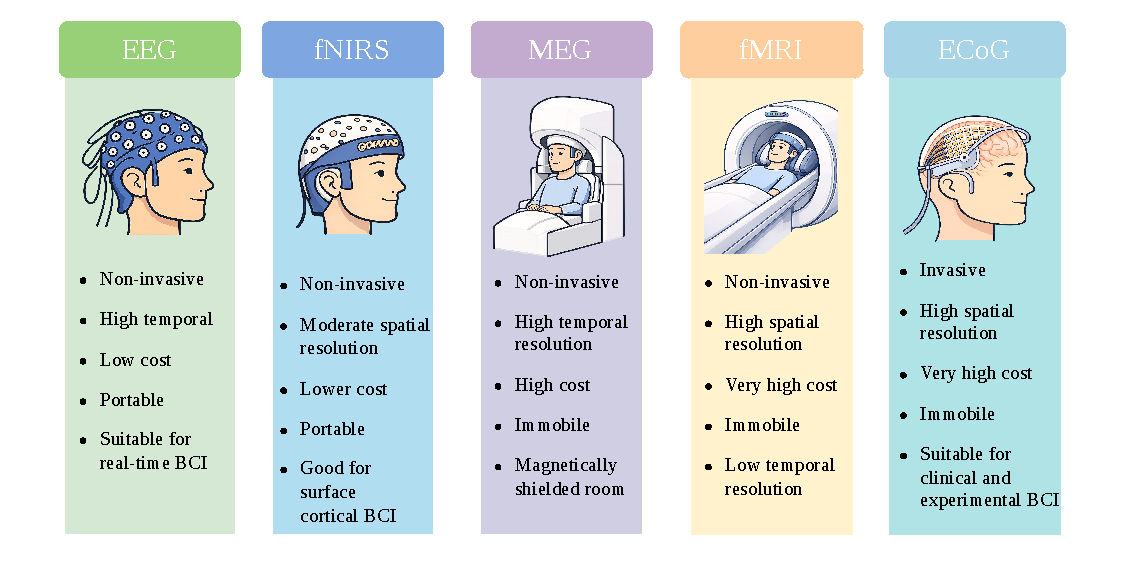
\includegraphics[width=\linewidth]{Figures/Motivacion 2.pdf}
    \caption{Overview of \gls{bci} acquisition technologies, including invasive and non-invasive modalities (\gls{eeg}, \gls{fnirs}, \gls{meg}, \gls{fmri}, and \gls{ecog}), highlighting their main trade-offs in terms of invasiveness, cost, portability, and spatial--temporal resolution.}
    \label{fig:Motivation2}
\end{figure}

In this context, \gls{eeg} has consolidated itself as a foundational technology for \gls{bci} implementation. \gls{eeg} captures electrical brain activity through scalp-mounted electrodes and enables the analysis of neural dynamics with millisecond-level temporal resolution. These characteristics support the extraction of \gls{erp} and other neurophysiological markers widely used to assess cognitive and motor functions~\cite{electronics14153106}. As a result, \gls{eeg} has become the technological backbone of many modern \gls{bci} platforms, enabling the decoding of neural activity to control external devices without requiring muscular involvement~\cite{lionakis2023trends}. Among the available paradigms, \gls{mi}—the mental rehearsal of movement without physical execution—has demonstrated notable clinical potential in post-stroke rehabilitation, neuroprosthetic control, and assistive technologies such as robotic wheelchairs and virtual spelling systems~\cite{s23052798}. Figure~\ref{fig:Motivation1} provides an overview of the conventional \gls{eeg}-based \gls{bci} pipeline, illustrating the main processing stages from signal acquisition and preprocessing to feature extraction, classification, and control or feedback generation.

\begin{figure}[H]
    \centering
    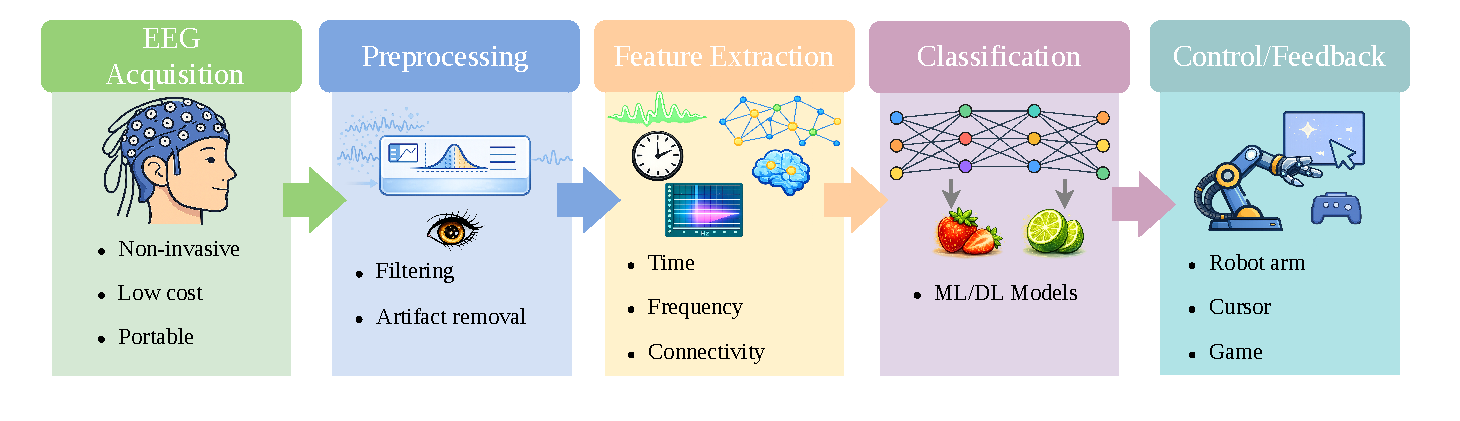
\includegraphics[width=\linewidth]{Figures/Motivation 1.pdf}
    \caption{Conventional \gls{eeg}-based \gls{bci} pipeline, illustrating the main stages from signal acquisition and preprocessing to feature extraction, classification, and control or feedback generation.}
    \label{fig:Motivation1}
\end{figure}

Beyond healthcare, \glspl{bci} have also demonstrated significant impact in educational and inclusion-oriented applications. In this context, Figure~\ref{fig:MI-TDHA} illustrates the two primary \gls{eeg} application paradigms addressed in this doctoral research, namely Motor Imagery--based
\gls{bci} decoding and \gls{eeg}-based \gls{adhd} detection. Studies report improvements in concentration, attentional focus, and engagement~\cite{djamal2020brain}, as well as promising results in the assessment and support of \gls{adhd}~\cite{maya2022hmm}. Moreover, \glspl{bci} have been integrated into pedagogical contexts to foster language comprehension and cognitive training in both children and older adults~\cite{bonnet2022kinesthetic}. These developments reinforce the societal value of \glspl{bci} by connecting health-oriented objectives (\gls{sdg3}) with education-oriented goals (\gls{sdg4}), underscoring the importance of affordable, scalable, and culturally adaptable neurotechnologies for diverse populations~\cite{nair2021engineering,de2018agenda}.

\begin{figure}[h]
    \centering
    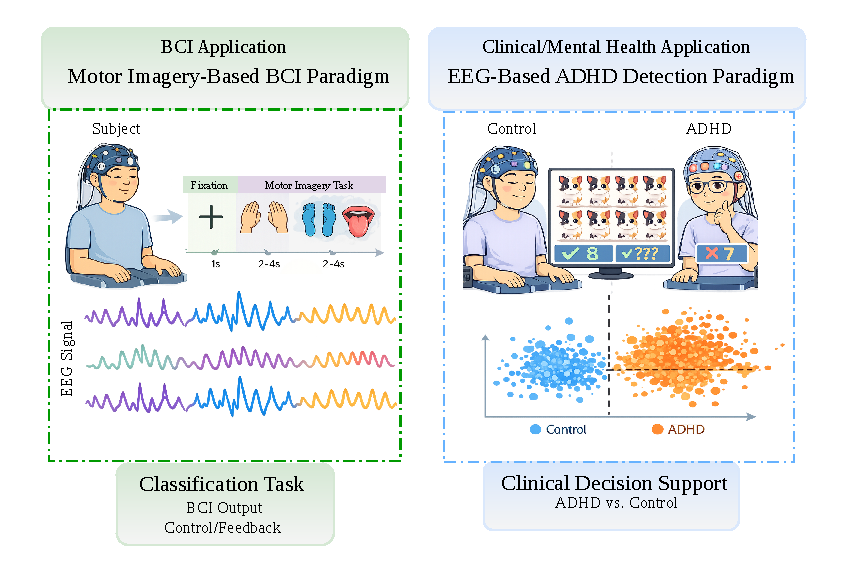
\includegraphics[width=\linewidth]{Figures/MI-TDHA.pdf}
    \caption{Overview of the two primary \gls{eeg} application paradigms addressed in this doctoral research. 
    Left: \gls{mi}--based \gls{eeg} \gls{bci} paradigm, where a subject performs imagined motor tasks and the resulting \gls{eeg} signals are used for classification and control or feedback generation. 
    Right: \gls{eeg}-based \gls{adhd} detection paradigm, where brain activity recorded during attention-demanding cognitive tasks is analyzed to support clinical decision-making by distinguishing between \gls{adhd} and control subjects.}
    \label{fig:MI-TDHA}
\end{figure}

The rapid advancement of \gls{ai} and \gls{ml} has further strengthened the development of \gls{bci} systems~\cite{lotte2018review}. By enabling data-driven modeling of complex neural dynamics, AI-based approaches have expanded the capacity of \glspl{bci} to learn discriminative patterns directly from neurophysiological signals~\cite{craik2019deep}. Deep learning architectures, representation learning strategies, and adaptive models have become central components of modern \gls{bci} pipelines, allowing systems to evolve beyond handcrafted features toward more flexible and autonomous solutions~\cite{schirrmeister2017deep,roy2019deep}. Figure~\ref{fig:Motivation3} provides an overview of the integration of \gls{ai} and \gls{ml} within the \gls{eeg}-based \gls{bci} pipeline, emphasizing data-driven representation learning, adaptive modeling, interpretability, and decision-making processes.

\begin{figure}[H]
    \centering
    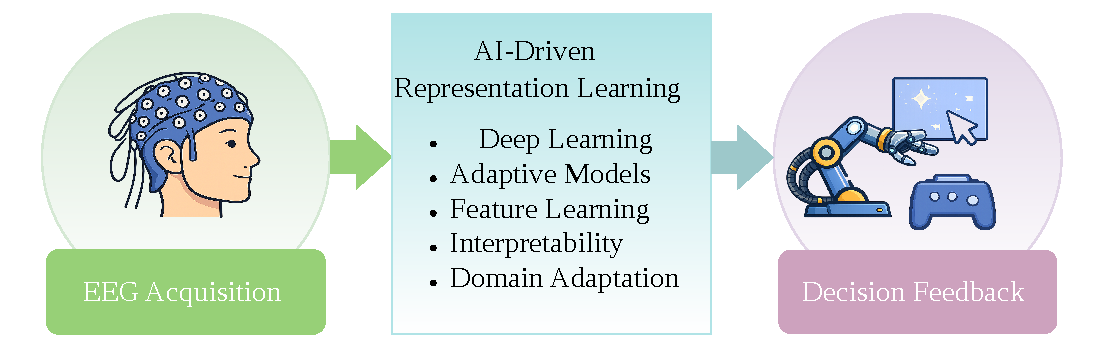
\includegraphics[width=\linewidth]{Figures/Motivation 3.pdf}
    \caption{Integration of \gls{ai} and \gls{ml} within \gls{eeg}-based \gls{bci} systems, emphasizing data-driven representation learning, adaptive modeling, interpretability, and decision-making processes.}
    \label{fig:Motivation3}
\end{figure}

The convergence of \gls{ai} and \gls{bci} technologies has opened new opportunities for the diagnosis, monitoring, and treatment of neurological and neurodevelopmental conditions~\cite{Kaboodvand2020ADHDNetworks,Shao2018ADHD}. In particular, data-driven \glspl{bci} have been explored as complementary tools for characterizing brain dynamics associated with cognitive deficits and for supporting personalized assessment and longitudinal monitoring~\cite{Kaboodvand2020ADHDNetworks}. Among these conditions, \gls{adhd} represents a pressing applied challenge, as objective and adaptive tools are required to better characterize attention, impulsivity, and hyperactivity across developmental stages~\cite{Shao2018ADHD}. Evidence further suggests that \glspl{bci}, perceptual technologies, and serious games can enhance engagement and adherence during both assessment and intervention, complementing traditional clinical and educational practices~\cite{maya2022hmm}. In this context, AI-driven \gls{eeg} analysis offers a promising avenue to support more objective, interpretable, and scalable approaches for \gls{adhd}-oriented assessment and monitoring~\cite{Kaboodvand2020ADHDNetworks}.

Addressing these emerging needs requires sustained methodological development grounded in both signal processing and \gls{ml} expertise. In response to these societal and technological needs, the \gls{gcpds} at the Universidad Nacional de Colombia has developed a sustained research line focused on neurophysiological signal analysis and the design of \gls{ml} methodologies for diagnosis, monitoring, and cognitive decoding based on \gls{eeg} data. Early contributions from the group explored kernel-based learning strategies to enhance the discrimination of neurophysiological patterns in biomedical signals, establishing a foundation for robust \gls{eeg}-based classification frameworks~\cite{Cardenas2017Kernel,Cardenas2017Enhanced}. These approaches emphasized the importance of capturing nonlinear relationships in brain signals while preserving interpretability and computational efficiency.

Building upon this foundation, subsequent work from \gls{gcpds} extended these methodologies toward clinical and applied scenarios, including cognitive assessment and neurological condition monitoring. In particular, adaptive \gls{ml} models were proposed to address variability across subjects and sessions in real-world settings, reinforcing the relevance of data-driven \gls{eeg} analysis for diagnosis and monitoring~\cite{Collazos2019Alzheimer,Collazos2019Instance}. In parallel, the group investigated \gls{eeg}-based monitoring in dynamic and non-stationary environments, demonstrating the feasibility of extracting meaningful neurophysiological information under realistic operating conditions~\cite{Pulgarin2017Kinematic}.

As the research trajectory evolved, \gls{gcpds} also contributed to advances in explainability and functional connectivity for \gls{eeg} classification. Representative examples include approaches that leverage class activation maps and canonical correlation analysis to provide multimodal interpretability in deep learning models for \gls{mi} classification~\cite{loaiza2024multimodal}, as well as kernel cross-spectral functional connectivity networks designed for \gls{eeg}-based \gls{mi} decoding~\cite{garcia2023kcsfcnet}. More recently, this research line has continued to evolve toward deep learning approaches that integrate connectivity-aware representations and information-theoretic principles for \gls{eeg} analysis, including transformer-based models with multi-scale Gaussian connectivity for neurodevelopmental applications such as \gls{adhd} detection~\cite{salazar2025tgar}. Collectively, these contributions reflect a coherent and evolving trajectory that spans kernel methods, adaptive learning, explainability, connectivity analysis, and deep learning, with applications in cognitive assessment, clinical monitoring, and neurodevelopmental disorders.

In summary, this doctoral research is motivated by the need to develop \gls{eeg}-based \gls{bci} systems that go beyond accuracy, achieving robustness, generalizability, and interpretability to ensure reliable performance across users and contexts. By integrating \gls{ai}-driven modeling with neurophysiological principles, {this doctoral research} aims to advance adaptive and explainable \gls{bci} frameworks for \gls{mi} and related neurocognitive applications, addressing fundamental challenges such as noise sensitivity, nonlinear brain dynamics, and inter- and intra-subject variability.

In this sense, the present doctoral thesis is conducted within the framework of the program \gls{acemate} (Project No. 91908), funded by the \gls{minciencias}, which articulates clinical and community-based interventions with scientific and technological developments aimed at strengthening mental health care in prioritized regions of the country. From a clinical perspective, \gls{acemate} seeks to address the need for objective tools that complement the assessment and follow-up of disorders associated with impulsivity, while, from a technological standpoint, it promotes the use of \gls{ai}–based approaches to support diagnosis, intervention, and longitudinal monitoring. In this context, this thesis contributes specifically through the development of computational methodologies based on machine learning and advanced processing of \gls{eeg} signals, oriented toward the characterization of neurophysiological patterns associated with both \gls{mi} paradigms and neurocognitive conditions related to impulsivity, such as \gls{adhd}. These methodologies support the construction of low-cost, portable, and scalable systems that reinforce the regional clinical impact and technological sustainability of the \gls{acemate} program.
\section{Problem Statement}\label{sec:problem_statement} 

\gls{eeg} is one of the most widely adopted technologies for \gls{mi}--based \glspl{bci} due to its non-invasive nature, low cost, portability, and high temporal resolution~\cite{singh2021comprehensive}. However, \gls{eeg} signals are intrinsically affected by structural and physiological limitations that hinder their effective exploitation in real-world applications. In particular, low spatial resolution, high susceptibility to noise and physiological artifacts, and volume conduction effects complicate the localization and physiological interpretation of cortical sources~\cite{wang2019eeg}. Furthermore, the nonlinear and nonstationary nature of \gls{eeg} signals poses additional challenges for robust modeling and analysis, limiting the reliability and interpretability of conventional \gls{eeg}-based \gls{bci} systems, especially in clinical and rehabilitation contexts where stable and explainable neural decoding is required~\cite{bouazizi2024interpretability}.

Beyond signal-level limitations, \gls{eeg}-based \glspl{bci} are strongly affected by pronounced inter-subject and intra-subject variability, leading to heterogeneous neural activation patterns across users and recording sessions~\cite{kim2023bridging,maswanganyi2022statistical}. This variability hampers generalization, promotes subject-dependent models, and contributes to the well-known BCI illiteracy phenomenon, where a significant proportion of users fail to achieve reliable control~\cite{saha2020intra,horowitz2021external}. Although deep learning approaches have improved decoding performance, many existing models rely on rigid or opaque representations that limit neurophysiological interpretability and fail to capture dynamic and nonlinear dependencies between \gls{eeg} channels~\cite{shoka2019literature,zhang2015bayesian}. These limitations highlight the need for connectivity-aware and interpretable learning frameworks capable of modeling complex brain interactions while improving robustness and generalization in \gls{mi}-based \gls{bci} systems~\cite{rolls2022effective}.

In this context, the following subsections provide a detailed analysis of the main challenges addressed in this thesis within the scope of EEG-based BCI systems, focusing on noisy data and low spatial resolution (Subsection~\ref{sec:Noisy}), nonlinear and nonstationary EEG channel dependencies (Subsection~\ref{sec:nonlinear}), and high inter- and intra-subject variability (Subsection~\ref{sec:variability}).

\subsection{Noisy data and low spatial resolution}\label{sec:Noisy}


One of the most critical limitations of \gls{eeg}-based \gls{bci} systems is their inherently low spatial resolution, which stems from the physical process by which neural electrical activity propagates from cortical sources to scalp electrodes. Due to volume conduction effects, \gls{eeg} signals traverse multiple tissue layers with heterogeneous conductivities, such as the cerebrospinal fluid, skull, and scalp, before being recorded. This phenomenon leads to spatial blurring and mixing of neural sources across electrodes, making it difficult to accurately localize task-related cortical activations~\cite{wang2019eeg}, as schematically illustrated in Figure~\ref{fig:problem1}. As a consequence, spatial specificity is significantly reduced compared to imaging modalities such as \gls{fmri} or \gls{meg}, limiting the effectiveness of \gls{eeg}-based \glspl{bci} in applications that require precise discrimination of motor and sensorimotor regions and impairing the interpretability of learned representations~\cite{electronics12122743,pan2025enhancing}. This challenge is particularly critical in \gls{mi}-based \gls{bci} paradigms and neurodevelopmental conditions such as \gls{adhd}, where motor-related cortical activations tend to be weaker, more diffuse, and highly variable, further exacerbating source localization uncertainty and reducing the reliability of neurophysiological interpretation~\cite{alnuaimi2022adhdmi}.

\begin{figure}[H]
    \centering
    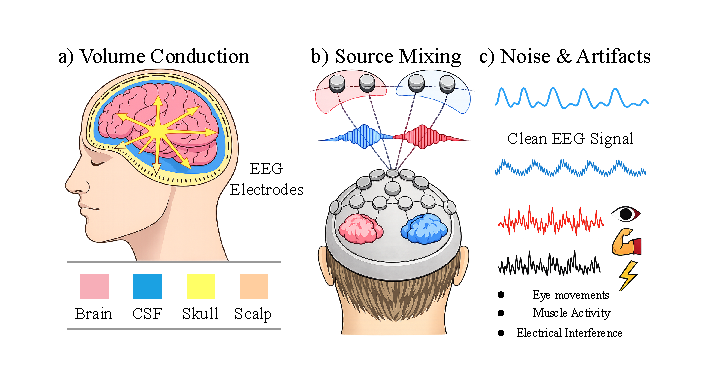
\includegraphics[width=\linewidth]{Figures/Problem 1.pdf}
    \caption{Major factors limiting \gls{eeg} spatial specificity and signal quality: (a) volume conduction through CSF, skull, and scalp causes spatial smearing; (b) source mixing leads each electrode to record a linear combination of multiple cortical sources; and (c) physiological and environmental artifacts (e.g., eye movements, muscle activity, and electrical interference) degrade the signal-to-noise ratio.}
    \label{fig:problem1}
\end{figure}

In parallel with limited spatial resolution, \gls{eeg} recordings are highly vulnerable to noise and artifacts arising from both physiological and non-physiological sources, including ocular movements, muscle activity, head motion, and environmental interference~\cite{de2018agenda}. These contaminations often overlap spectrally with task-relevant rhythms, such as the $\mu$ and $\beta$ bands, which are fundamental for \gls{mi} decoding~\cite{pfurtscheller1999event}. As a result, the signal-to-noise ratio is substantially degraded, increasing intra- and inter-trial variability and reducing the robustness of conventional feature extraction and classification pipelines~\cite{bouazizi2024interpretability}. Although classical preprocessing techniques and spatial filtering methods can partially mitigate these effects, they remain sensitive to residual noise and spatial distortions, ultimately constraining the generalization capability and reliability of \gls{eeg}-based \gls{bci} systems in real-world and clinical settings~\cite{akuthota2023complete,pan2025enhancing}, particularly in \gls{mi}-based applications and populations with \gls{adhd}, where attentional fluctuations, involuntary movements, and reduced task compliance further degrade signal quality and stability~\cite{lenartowicz2018adhd}. These limitations motivate the need for representations that go beyond sensor-level activity and explicitly model inter-channel relationships, including their nonlinear and time-varying dynamics, to improve robustness and interpretability under noisy and low-resolution \gls{eeg} conditions.

\subsection{Nonlinear and Nonstationary \gls{eeg}Channel dependencies}\label{sec:nonlinear}

\gls{eeg} signals exhibit pronounced nonlinear and nonstationary behavior, reflecting the intrinsic dynamics of underlying neural processes and their continuous adaptation to cognitive states, stimuli, and task demands~\cite{breakspear2017dynamic}. In \gls{mi} paradigms, the statistical properties of \gls{eeg} signals vary over time due to changes in attention, mental strategy, and neural engagement, which violates the assumptions of stationarity commonly adopted by classical signal processing and machine learning methods~\cite{shoka2019literature}. These effects are further exacerbated in practical \gls{eeg}-based \glspl{bci}, where variability across trials, sessions, and subjects introduces additional sources of nonstationarity that challenge reliable decoding. Moreover, neural interactions across cortical regions are inherently nonlinear, as they arise from complex synaptic mechanisms, recurrent feedback loops, and cross-frequency interactions. Such nonlinear dynamics are particularly relevant in neurodevelopmental conditions such as \gls{adhd}. {Clinically, ADHD is characterized by persistent patterns of inattention and/or hyperactivity--impulsivity that interfere with functioning or development~\cite{APA2022DSM5TR}.} In this context, altered
attentional control and fluctuating cognitive states have been associated with abnormal neural coupling and increased temporal variability. These characteristics limit the effectiveness of linear connectivity measures and static feature representations, which are unable to fully capture the evolving and nonlinear dependencies that govern inter-channel \gls{eeg} dynamics~\cite{rolls2022effective}. These nonlinear, nonstationary, and time-evolving inter-channel interactions are schematically illustrated in Figure~\ref{fig:problem2}.

Beyond nonstationarity, \gls{eeg} channels interact through time-delayed and directed relationships that reflect causal information flow within brain networks~\cite{rolls2022effective}. In \gls{eeg}-based \glspl{bci}, particularly those relying on \gls{mi} decoding, capturing such directed interactions is essential for distinguishing task-relevant sensorimotor activations from background or confounding activity. Conventional correlation-based or symmetric connectivity measures fail to adequately characterize these interactions, as they cannot distinguish between driving and responding channels nor capture nonlinear dependencies~\cite{zhang2015bayesian}. This limitation is especially critical in high-variability scenarios, including subject-independent \gls{bci} operation and neurodevelopmental studies involving \gls{adhd}, where spurious or volume-conduction-driven correlations may obscure meaningful patterns of effective connectivity. Information-theoretic approaches, such as \gls{te}, have been proposed to quantify directed and nonlinear interactions between time series~\cite{schreiber2000measuring,staniek2008symbolic}. However, their practical application to \gls{eeg} signals is hindered by high sensitivity to noise, high data dimensionality, and the need for explicit probability density estimation, which limits their effectiveness in real-world \gls{bci} scenarios characterized by nonstationary and noisy \gls{eeg} recordings~\cite{pereda2005nonlinear}.These nonlinear, nonstationary, and directed inter-channel dependencies are not only task- and state-dependent, but also vary substantially across individuals and recording sessions, naturally giving rise to pronounced inter- and intra-subject variability in \gls{eeg}-based \glspl{bci}.

\begin{figure}[h]
    \centering
    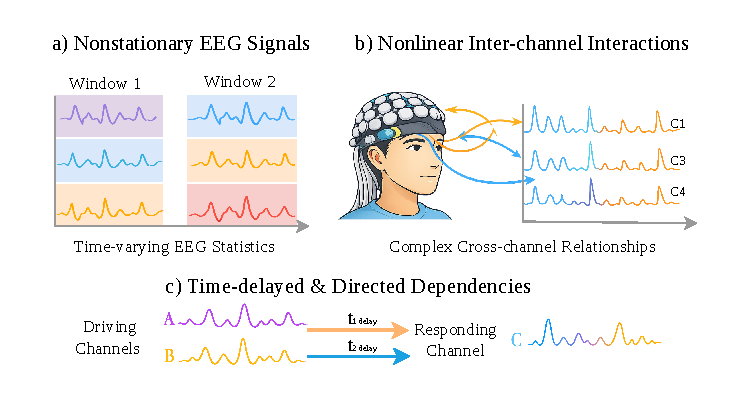
\includegraphics[width=\linewidth]{Figures/Problem 2.pdf}
    \caption{Illustration of nonlinear and nonstationary \gls{eeg} channel dependencies.
    (a) Nonstationary \gls{eeg} signals showing time-varying statistical properties across analysis windows.
    (b) Nonlinear inter-channel interactions, illustrating complex cross-channel relationships between \gls{eeg} signals that cannot be fully described by simple linear dependencies.
    (c) Time-delayed and directed dependencies between \gls{eeg} channels, where the past activity of multiple driving channels may contribute information to the activity of a responding channel after different temporal delays, highlighting asymmetric information flow that cannot be captured by linear or symmetric connectivity measures.}
    \label{fig:problem2}
\end{figure}

\subsection{High inter- and intra-subject variability}\label{sec:variability}

Inter-subject variability constitutes a fundamental limitation in \gls{eeg}-based learning systems, as neural responses exhibit strong heterogeneity across individuals, even when identical tasks are performed under controlled experimental conditions. In \gls{eeg}-based \glspl{bci}, particularly those relying on \gls{mi} paradigms, this variability is amplified by differences in motor imagery strategies, cortical organization, and cognitive engagement across users~\cite{lotte2018review}. \gls{eeg} signals therefore exhibit substantial inter-subject variability, and clinical conditions such as \gls{adhd} further present heterogeneous neurocognitive profiles, leading to highly subject-dependent \gls{eeg} signatures~\cite{arnett2022framework}. As a consequence, models trained on limited or homogeneous cohorts frequently experience significant performance degradation when evaluated on unseen subjects or new recording conditions, revealing a strong vulnerability to domain shift and subject-specific noise~\cite{al2025emotion}. This behavior indicates that many existing approaches inadvertently learn dataset-specific artifacts rather than invariant neurophysiological structures, thereby limiting their generalization capability in subject-independent \gls{bci} scenarios~\cite{wang2024dmmr}. The impact of inter- and intra-subject variability on model generalization and the resulting risk of overfitting in subject-independent settings are schematically illustrated in Figure~\ref{fig:problem3}.

\begin{figure}[H]
    \centering
    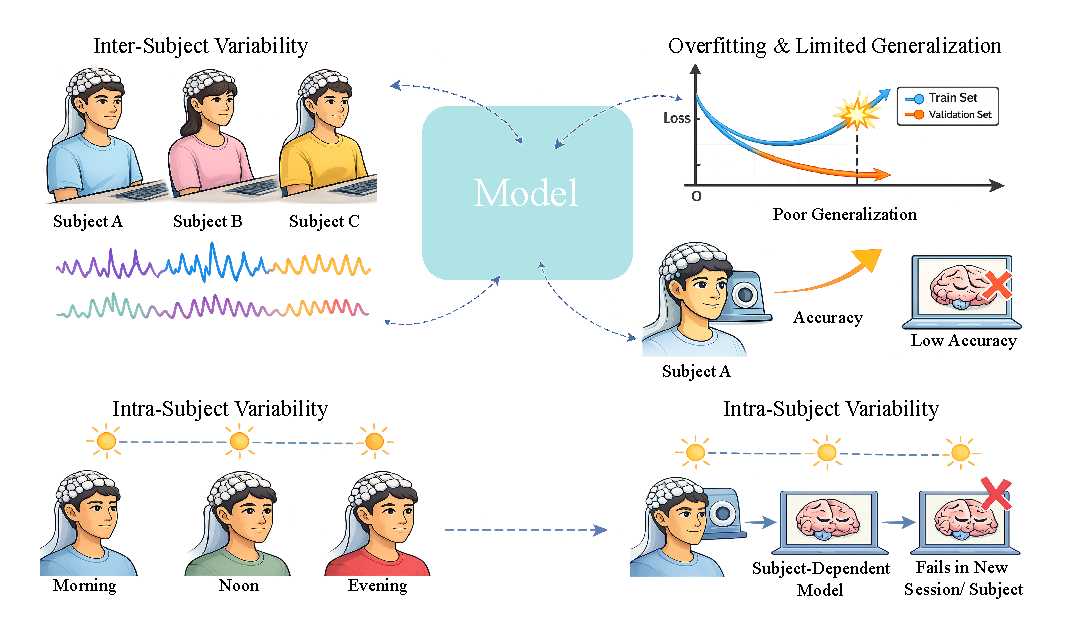
\includegraphics[width=\linewidth]{Figures/Problem 3.pdf}
    \caption{Inter- and intra-subject variability in \gls{eeg}-based \gls{bci} systems leading to overfitting and limited subject-independent generalization.}
    \label{fig:problem3}
\end{figure}

In addition to inter-subject differences, intra-subject variability introduces an additional challenge for robust \gls{eeg} modeling. \gls{eeg} signals recorded from the same individual may vary considerably across sessions due to fluctuations in attention, fatigue, emotional state, and subtle changes in acquisition conditions, resulting in nonstationary signal distributions over time~\cite{al2025emotion}. Such variability is particularly pronounced in real-world \gls{eeg}-based \glspl{bci} and in neurodevelopmental populations such as \gls{adhd}, where altered attentional control and increased behavioral variability have been shown to induce strong trial-to-trial and session-to-session fluctuations in neural activity~\cite{lenartowicz2018adhd}. This variability exacerbates the risk of overfitting, as learning algorithms may adapt to session-specific or noise-related patterns rather than stable neurophysiological features. Consequently, performance observed under optimistic or subject-dependent validation protocols often fails to generalize across sessions or recording conditions, reinforcing the vulnerability to domain shift and dataset-specific artifacts that has been consistently reported in subject-independent evaluations~\cite{wang2024dmmr}.

\subsection{Research Question}

\gls{eeg}-based \gls{bci} models face substantial constraints in their ability to generalize when exposed to distribution shifts across subjects, sessions, and recording conditions. These limitations are exacerbated by intrinsic properties of \gls{eeg} signals, including low spatial resolution induced by volume conduction effects, high susceptibility to noise and artifacts, and the nonlinear and nonstationary nature of brain dynamics. The interplay between signal degradation, heterogeneous neural patterns, and strong inter- and intra-subject variability undermines both the discriminative capability and the neurophysiological interpretability of existing learning models. Despite the adoption of deep learning, connectivity-based representations, and domain adaptation strategies, significant challenges remain in achieving robust, generalizable, and interpretable \gls{eeg} representations under real-world conditions.

This landscape motivates the research question: \textbf{How can an integrated and interpretable deep learning framework be designed for \gls{eeg}-based \gls{bci} systems to robustly model nonlinear and directed brain connectivity while improving generalization across subjects and sessions and mitigating the effects of noise and subject-specific variability?}
\section{State of the Art}

\subsection{Classical \gls{eeg}-based Models}

Early developments of \gls{bci} systems based on \gls{eeg} and \gls{mi} paradigms have been fundamentally constrained by the physical and physiological properties of \gls{eeg} signal acquisition. Due to volume conduction effects, neural electrical activity generated at cortical sources propagates through heterogeneous tissue layers before being recorded at the scalp, leading to spatial blurring and mixing of neural sources across electrodes \cite{wang2019eeg}. This phenomenon severely limits the spatial resolution of \gls{eeg} recordings, reducing the ability to localize task-related cortical activations and impairing the discriminative power of sensor-level representations. Consequently, early \gls{bci} systems relied heavily on signal processing techniques designed to enhance task-relevant information while attempting to suppress noise and spatial interference \cite{singh2021comprehensive}.

Classical \gls{eeg} decoding pipelines typically employ spectral and time--frequency transformations to extract features associated with \gls{mi} activity. Methods based on Fourier analysis and wavelet decompositions have been widely used to isolate oscillatory patterns within the $\mu$ and $\beta$ bands, which are known to reflect sensorimotor rhythms modulated during \gls{mi} tasks \cite{pfurtscheller1999event,singh2021comprehensive}. While these representations partially address the nonstationary nature of \gls{eeg} signals by enabling localized spectral analysis, they do not inherently resolve the spatial ambiguity introduced by volume conduction, as frequency-domain features remain derived from mixed sensor-level signals.

To enhance spatial discriminability, classical approaches frequently incorporate spatial filtering techniques, most notably \gls{csp} and its extensions, such as \gls{fbcsp}. By projecting multichannel \gls{eeg} signals into a discriminative subspace that maximizes variance differences between classes, \gls{csp}-based methods can improve signal-to-noise ratio and classification accuracy under controlled experimental conditions \cite{wang2019eeg}. However, these methods rely on linear assumptions and are highly sensitive to noise, electrode placement, and inter-subject variability. Furthermore, their dependence on predefined frequency bands and subject-specific calibration procedures significantly limits their robustness and generalization capability, particularly in subject-independent or clinical scenarios \cite{maswanganyi2022statistical,saha2020intra}.

Additional preprocessing strategies, including surface Laplacian filtering, have been proposed to mitigate the effects of volume conduction by emphasizing local cortical activity and suppressing global signal components. Although such techniques can improve spatial resolution at the sensor level, they remain vulnerable to residual noise and cannot fully disentangle underlying cortical sources, resulting in only partial mitigation of spatial mixing \cite{wang2019eeg,pan2025enhancing}. As a result, classical \gls{eeg}-based \gls{bci} systems often exhibit limited robustness and reduced interpretability, especially when deployed in real-world environments characterized by high noise levels and pronounced inter-subject variability \cite{bouazizi2024interpretability}.{These main limitations of classical \gls{eeg}-based decoding pipelines are summarized in Figure~\ref{fig:classical_eeg_models}.}

% \begin{figure}[H]
% \centering
% \begin{tikzpicture}[x=\linewidth,y=1.2cm,line width=0.9pt,font=\normalsize]

% % ===== spacing =====
% \def\labelpad{0.015}
% \def\topbot{0.10}
% \def\dy{0.9}
% \def\yA{1.0}
% \def\gapBlocks{0.9} % <<< gap vertical (en "unidades y") entre grupos
% \def\amp{3pt}

% \pgfmathsetmacro{\yB}{\yA - (2 + \gapBlocks)*\dy}

% % ===== styles =====
% \tikzset{
%   brace/.style={
%     draw=none,
%     postaction={draw,decorate,decoration={brace,mirror,raise=0pt,amplitude=\amp}}
%   },
%   lab/.style={anchor=east,fill=white,inner sep=1.2pt,align=center},
%   glab/.style={anchor=east,fill=white,inner sep=1.2pt},
%   item/.style={anchor=west,text width=0.50\linewidth}
% }

% % ===== column positions =====
% \pgfmathsetmacro{\xMain}{0.30}
% \pgfmathsetmacro{\xInner}{0.53}
% \pgfmathsetmacro{\xText}{0.55}

% % ===== labels =====
% \def\Main{Classical EEG-based \\ Models}
% \def\A{Spectral / Spatial}
% \def\B{Classification}

% % ===== items =====
% \def\Aone{Fourier / Wavelet features $\rightarrow$
% \textcolor{red}{limited spatial specificity}}

% \def\Atwo{STFT / Time--frequency $\rightarrow$
% \textcolor{red}{sensor-level source mixing}}

% \def\Athree{CSP / FBCSP $\rightarrow$
% \textcolor{red}{linear assumptions, noise sensitivity}}

% \def\Afour{Surface Laplacian $\rightarrow$
% \textcolor{red}{partial mitigation of volume conduction}}

% \def\Bone{LDA $\rightarrow$
% \textcolor{red}{subject-dependent calibration}}

% \def\Btwo{SVM $\rightarrow$
% \textcolor{red}{poor generalization across subjects}}

% % ===== main brace =====
% \draw[brace] (\xMain,\yA+1.5*\dy+\topbot) -- (\xMain,\yB-0.5*\dy-\topbot);
% \node[lab] at (\xMain-\labelpad, {(\yA+\yB)/2}) {\Main};

% % ===== group braces (SEGUND A ETAPA: separados de verdad) =====

% % Spectral/Spatial brace (4 items: yA±1.5dy)
% \draw[brace]
%   (\xInner,\yA+1.5*\dy+\topbot) --
%   (\xInner,\yA-1.5*\dy-\topbot);

% % Classification brace (2 items: yB±0.5dy)
% \draw[brace]
%   (\xInner,\yB+0.5*\dy+\topbot) --
%   (\xInner,\yB-0.5*\dy-\topbot);

% % ===== group labels =====
% \node[glab] at (\xInner-0.01,\yA) {\A};
% \node[glab] at (\xInner-0.05,\yB) {\B};

% % ===== items =====
% \node[item] at (\xText,\yA+1.5*\dy) {\Aone};
% \node[item] at (\xText,\yA+0.5*\dy) {\Atwo};
% \node[item] at (\xText,\yA-0.5*\dy) {\Athree};
% \node[item] at (\xText,\yA-1.5*\dy) {\Afour};

% \node[item] at (\xText,\yB+0.5*\dy) {\Bone};
% \node[item] at (\xText,\yB-0.5*\dy) {\Btwo};

% \end{tikzpicture}
% \vspace{-2em}
% \caption{Fundamental limitations of classical \gls{eeg}-based models for \gls{mi} decoding. Classical pipelines rely on handcrafted spectral and spatial features combined with shallow classifiers, which remain constrained by low spatial resolution, linear assumptions, sensitivity to noise, and strong subject dependence.}
% \label{fig:classical_eeg_models}
% \end{figure}

%-----------------------------------------------
\begin{figure}[htbp]
\centering

\begin{tikzpicture}[
    x=\linewidth,
    y=1.1cm,
    line width=0.9pt,
    font=\small
]

% ===== Spacing =====
\def\labelpad{0.015}
\def\topbot{0.10}
\def\dy{1.05}
\def\yA{1.0}
\def\gapBlocks{0.85}
\def\amp{3pt}

\pgfmathsetmacro{\yB}{\yA-(2+\gapBlocks)*\dy}

% ===== Styles =====
\tikzset{
    brace/.style={
        draw=none,
        postaction={
            draw,
            decorate,
            decoration={
                brace,
                mirror,
                raise=0pt,
                amplitude=\amp
            }
        }
    },
    lab/.style={
        anchor=east,
        fill=white,
        inner sep=1.2pt,
        align=center
    },
    glab/.style={
        anchor=east,
        fill=white,
        inner sep=1.2pt,
        align=center
    },
    item/.style={
        anchor=west,
        text width=0.43\linewidth,
        align=left
    }
}

% ===== Column positions =====
\pgfmathsetmacro{\xMain}{0.30}
\pgfmathsetmacro{\xInner}{0.53}
\pgfmathsetmacro{\xText}{0.55}

% ===== Labels =====
\def\Main{Classical EEG-Based\\Models}
\def\A{Spectral/Spatial}
\def\B{Classification}

% ===== Items =====
\def\Aone{Fourier/Wavelet features $\rightarrow$
\textcolor{red}{limited spatial specificity}}

\def\Atwo{STFT/time--frequency features $\rightarrow$
\textcolor{red}{sensor-level source mixing}}

\def\Athree{CSP/FBCSP $\rightarrow$
\textcolor{red}{linear assumptions and noise sensitivity}}

\def\Afour{Surface Laplacian $\rightarrow$
\textcolor{red}{partial mitigation of volume conduction}}

\def\Bone{LDA $\rightarrow$
\textcolor{red}{subject-dependent calibration}}

\def\Btwo{SVM $\rightarrow$
\textcolor{red}{limited generalization across subjects}}

% ===== Main brace =====
\draw[brace]
    (\xMain,\yA+1.5*\dy+\topbot) --
    (\xMain,\yB-0.5*\dy-\topbot);

\node[lab]
    at (\xMain-\labelpad,{(\yA+\yB)/2})
    {\Main};

% ===== Group braces =====

% Spectral/Spatial group
\draw[brace]
    (\xInner,\yA+1.5*\dy+\topbot) --
    (\xInner,\yA-1.5*\dy-\topbot);

% Classification group
\draw[brace]
    (\xInner,\yB+0.5*\dy+\topbot) --
    (\xInner,\yB-0.5*\dy-\topbot);

% ===== Group labels =====
\node[glab] at (\xInner-0.01,\yA) {\A};
\node[glab] at (\xInner-0.05,\yB) {\B};

% ===== Spectral/Spatial items =====
\node[item] at (\xText,\yA+1.5*\dy) {\Aone};
\node[item] at (\xText,\yA+0.5*\dy) {\Atwo};
\node[item] at (\xText,\yA-0.5*\dy) {\Athree};
\node[item] at (\xText,\yA-1.5*\dy) {\Afour};

% ===== Classification items =====
\node[item] at (\xText,\yB+0.5*\dy) {\Bone};
\node[item] at (\xText,\yB-0.5*\dy) {\Btwo};

\end{tikzpicture}

\vspace{0.8em}

\caption{Fundamental limitations of classical
\gls{eeg}-based models for \gls{mi} decoding. Classical pipelines
rely on handcrafted spectral and spatial features combined with
shallow classifiers, which remain constrained by low spatial
resolution, linear assumptions, sensitivity to noise, and strong
subject dependence.}
\label{fig:classical_eeg_models}

\end{figure}
%-----------------------------------------------

\subsection{Connectivity-based Methods for  \gls{eeg}-based \gls{bci}}

Beyond classical spectral and spatial pipelines, connectivity-based methods have emerged as a key strategy for modeling inter-channel interactions in \gls{eeg}-based \gls{bci} systems, particularly to address the nonlinear and nonstationary nature of neural dynamics \cite{shoka2019literature,singh2021comprehensive}. {The main challenges that motivate this connectivity-based perspective, including temporal drift, linear-connectivity limitations, volume conduction effects, and the need for directed nonlinear measures, are summarized in Figure~\ref{fig:nonlinear_nonstationary_dependencies}.} {\gls{eeg} signals reflect the collective activity of large-scale neural populations whose interactions evolve over time as a function of attention, fatigue, and task engagement~\cite{wang2019eeg}.} In paradigms such as \gls{mi} and in \gls{eeg}-based applications targeting neurological and neurodevelopmental conditions, including \gls{adhd}, these temporal variations induce pronounced changes in the statistical properties of \gls{eeg} signals both within and across trials, violating the stationarity assumptions underlying many classical signal processing and machine learning approaches. As a result, representations derived from fixed temporal or spectral assumptions often fail to capture the dynamic structure of brain activity, limiting robustness and reliability \cite{singh2021comprehensive}.

Early attempts to model inter-channel relationships in \gls{eeg} primarily relied on linear and symmetric measures of functional connectivity, such as correlation, coherence, and phase-based metrics \cite{pereda2005nonlinear}. While these measures provide valuable insights into synchronized neural activity, they are inherently limited in their expressive power, as they assume linear interactions and fail to distinguish between driving and responding neural sources \cite{bastos2016tutorial}. Moreover, linear connectivity measures are particularly vulnerable to volume conduction effects, often producing spurious connections that reflect common-source artifacts rather than genuine neural interactions \cite{nunez1997eeg,vinck2011improved}. These limitations become especially critical in scenarios characterized by high inter- and intra-subject variability, such as \gls{mi}-based decoding and \gls{eeg}-based studies involving \gls{adhd}, where fluctuations in attention and cognitive state further complicate the reliable characterization of brain network dynamics.

To overcome these limitations, increasing attention has been devoted to information theoretic and causality-based measures capable of capturing nonlinear  and directed interactions between \gls{eeg} channels. Among these, \gls{te} has emerged as a principled framework for quantifying directed information flow between time series, enabling the identification of asymmetric and time-delayed dependencies that cannot be detected by correlation-based methods \cite{staniek2008symbolic}. By explicitly modeling how the past of one signal reduces uncertainty about the future of another, \gls{te} provides a more faithful representation of effective brain connectivity, closely aligning with the notion of neural communication and causal influence \cite{bastos2016tutorial,faes2017information}.

Despite its theoretical appeal, the practical application of \gls{te} to \gls{eeg} data remains challenging. Classical estimators require explicit probability density estimation, which is highly sensitive to noise, data length, and dimensionality \cite{vicente2011transfer}. These challenges are exacerbated in \gls{eeg} recordings, where limited trial counts, nonstationarity, and high-dimensional inter-channel interactions hinder reliable connectivity estimation \cite{zhang2015bayesian,faes2017information}. As a result, many studies restrict \gls{te} analysis to small subsets of channels or rely on simplified assumptions that compromise the fidelity of the inferred connectivity patterns.

More recently, research has explored kernel-based and embedding-based formulations to alleviate some of these challenges, enabling more robust estimation of nonlinear dependencies without explicit density modeling \cite{marinazzo2011kernel}. In parallel, deep learning approaches have begun to incorporate connectivity information as part of the feature representation, either by using precomputed connectivity matrices or by embedding interaction patterns directly into neural architectures \cite{li2019deep,rolls2022effective}. While these methods improve interpretability and provide richer representations of brain dynamics, they often rely on externally computed and fixed connectivity estimators, preventing joint optimization with the classification objective and limiting adaptability to task-specific dynamics.

\begin{figure}[H]
\centering
\begin{tikzpicture}[x=\linewidth,y=1.15cm,line width=0.9pt,font=\normalsize]

% ===== spacing =====
\def\labelpad{0.015}
\def\topbotMain{0.10}
\def\topbotInner{0.00}
\def\dy{1.1}
\def\yT{2.35}
\def\amp{3pt}
\def\vgap{0.12}

% ===== styles =====
\tikzset{
  brace/.style={
    draw=none,
    postaction={draw,decorate,decoration={brace,mirror,raise=0pt,amplitude=\amp}}
  },
  lab/.style={anchor=east,fill=white,inner sep=1.2pt,align=center},
  glab/.style={anchor=center,fill=white,inner sep=1.2pt,align=center},
  item/.style={anchor=west,text width=0.58\linewidth}
}

% ===== column positions =====
\pgfmathsetmacro{\xMain}{0.28}
\pgfmathsetmacro{\xInner}{0.56}
\pgfmathsetmacro{\xText}{0.56}
\pgfmathsetmacro{\xMid}{(\xMain+\xInner)/2}

% ===== labels =====
\def\Main{\shortstack{Connectivity-based\\\gls{eeg} Modeling\\Challenges}}

\def\GOne{\shortstack{Nonstationarity\\(temporal drift)}}
\def\GTwo{\shortstack{Linear\\connectivity}}
\def\GThree{\shortstack{Directed\\nonlinear\\measures}}

% ===== items =====
\def\Ione{State/attention/fatigue $\rightarrow$ \textcolor{red}{time-varying statistics, trial drift}}
\def\Itwo{Fixed temporal/spectral assumptions $\rightarrow$ \textcolor{red}{reduced robustness across trials/sessions}}

\def\Ithree{Correlation/coherence/phase metrics $\rightarrow$ \textcolor{red}{linear, symmetric (no directionality)}}
\def\Ifour{Volume conduction $\rightarrow$ \textcolor{red}{spurious connections, common-source artifacts}}

\def\Ifive{\gls{te} $\rightarrow$ \textcolor{red}{directed, time-lagged nonlinear dependencies}}
\def\Isix{Captures driving vs responding sources $\rightarrow$ \textcolor{red}{effective connectivity alignment}}

% ===== y positions (6 items) =====
\pgfmathsetmacro{\yZero}{\yT}
\pgfmathsetmacro{\yOne}{\yT-1*\dy}
\pgfmathsetmacro{\yTwo}{\yT-2*\dy}
\pgfmathsetmacro{\yThree}{\yT-3*\dy}
\pgfmathsetmacro{\yFour}{\yT-4*\dy}
\pgfmathsetmacro{\yFive}{\yT-5*\dy}

% ===== main brace =====
\draw[brace] (\xMain,\yZero+0.5*\dy+\topbotMain) -- (\xMain,\yFive-0.5*\dy-\topbotMain);
\node[lab] at (\xMain-\labelpad,{(\yZero+\yFive)/2}) {\Main};

% ===== group braces =====
\draw[brace] (\xInner,\yZero+0.5*\dy+\topbotInner) --
             (\xInner,\yOne-0.5*\dy-\topbotInner+\vgap);

\draw[brace] (\xInner,\yTwo+0.5*\dy+\topbotInner-\vgap) --
             (\xInner,\yThree-0.5*\dy-\topbotInner+\vgap);

\draw[brace] (\xInner,\yFour+0.5*\dy+\topbotInner-\vgap) --
             (\xInner,\yFive-0.5*\dy-\topbotInner);

% ===== group labels =====
\node[glab] at (\xMid,{(\yZero+\yOne)/2}) {\GOne};
\node[glab] at (\xMid,{(\yTwo+\yThree)/2}) {\GTwo};
\node[glab] at (\xMid,{(\yFour+\yFive)/2}) {\GThree};

% ===== items =====
\node[item] at (\xText,\yZero) {\Ione};
\node[item] at (\xText,\yOne) {\Itwo};

\node[item] at (\xText,\yTwo) {\Ithree};
\node[item] at (\xText,\yThree) {\Ifour};

\node[item] at (\xText,\yFour) {\Ifive};
\node[item] at (\xText,\yFive) {\Isix};

\end{tikzpicture}
\vspace{-1.2em}
\caption{Key challenges motivating connectivity-based modeling of nonlinear and nonstationary \gls{eeg} interactions in \gls{mi} decoding.}
\label{fig:nonlinear_nonstationary_dependencies}
\end{figure}

Overall, existing approaches to modeling nonlinear and nonstationary \gls{eeg} channel dependencies remain fragmented. Linear connectivity measures lack expressiveness, classical information-theoretic methods suffer from practical limitations, and hybrid deep learning solutions frequently decouple connectivity estimation from representation learning. These limitations underscore the need for integrated frameworks capable of capturing directed, nonlinear brain interactions in a data-driven and end-to-end manner, while maintaining robustness to noise and nonstationarity—an essential requirement for advancing reliable and interpretable \gls{eeg}-based \gls{bci} systems.

\subsection{\texorpdfstring{{Causality, Directed Predictability, and Effective Connectivity in EEG}}{Causality, Directed Predictability, and Effective Connectivity in EEG}}
\label{sec:causality_eeg}


The notion of causality in \gls{eeg} connectivity analysis must be interpreted with caution. In neuroscience and neuroimaging, terms such as \emph{Granger causality}, \emph{causal connectivity}, \emph{effective connectivity}, and \emph{directed information flow} are commonly used to describe directed statistical dependencies between neural time series. However, these terms do not necessarily imply causality in the strict interventional or 
mechanistic sense. Instead, they are usually grounded in the Wiener--Granger predictive framework, where a process is said to exert a causal influence on another if its past improves the prediction of the target process beyond the information contained in the target's own past~\cite{Granger1969,Seth2015Granger}.

Within this framework, Granger causality has been widely adopted in neuroscience as a data-driven tool for characterizing directed functional interactions and effective connectivity in neural systems~\cite{Friston2013Connectivity,Seth2015Granger}. Nevertheless, its interpretation depends on several assumptions, including temporal precedence, adequate sampling, stationarity or appropriate handling of nonstationarity, sufficient model order, and adequate conditioning on relevant observed variables
~\cite{Seth2015Granger,Barnett2017Subsampling,Stokes2017Problems}. Therefore, Granger-causal relations should be understood primarily as directed predictive dependencies, rather than definitive evidence of direct biophysical or interventional causal mechanisms~\cite{Seth2015Granger,Stokes2017Problems}.

\gls{te} extends this predictive perspective from an information-theoretic viewpoint. \gls{te} quantifies the information provided by the past of a source process about the future or present state of a target process, conditioned on the target's own past~\cite{Schreiber2000,Vicente2011TE}. Unlike classical linear Granger causality, \gls{te} is model-free and can capture nonlinear and asymmetric dependencies, which makes it particularly attractive for \gls{eeg} signals, whose dynamics are nonlinear, nonstationary, and time-dependent. Moreover, for Gaussian variables, \gls{te} and Granger causality have been shown to be formally equivalent, linking autoregressive and information-theoretic formulations of directed predictability~\cite{Barnett2009TEGC}.

Despite these advantages, \gls{te} does not solve the problem of causality in the strict sense. As an observational measure, \gls{te} remains susceptible to hidden common causes, indirect pathways, source mixing, volume conduction, sampling artifacts, finite-sample bias, and insufficient conditioning~\cite{Haufe2013EEGConnectivity,Bastos2016Pitfalls,TehraniSaleh2020TE}. These issues are especially relevant in scalp \gls{eeg}, where each sensor may record mixtures of multiple neural and non-neural sources. Consequently, a significant \gls{te} value should not be interpreted as proof of a direct anatomical or mechanistic causal pathway between \gls{eeg} channels.

Accordingly, this doctoral proposal adopts a cautious interpretation of causality. 
The proposed TEKTE-Net framework is not intended to infer true interventional 
causality from \gls{eeg} recordings. Rather, it aims to estimate nonlinear, 
time-delayed, and directed predictive dependencies among \gls{eeg} channels using 
a Takens-based kernel \gls{te} formulation. In this sense, although the terminology 
adopted in this work reflects a convention commonly used in neuroscience and 
\gls{eeg} connectivity analysis~\cite{Friston2013Connectivity,Seth2015Granger,
Vicente2011TE}, expressions such as \emph{causal influence}, \emph{causal structure}, 
or \emph{causal information flow}, when related to \gls{te}, should be understood in 
the predictive Wiener--Granger sense, rather than as causality in the strict 
interventional, counterfactual, or mechanistic sense established in modern causal 
inference~\cite{Pearl2009Causality,Peters2017Elements}. Therefore, the resulting 
connectivity patterns are interpreted as \gls{te}-based directed information flow or 
directed effective connectivity at the signal level, while explicitly acknowledging 
the limitations that prevent a strict causal interpretation.


\subsection{Modeling Strategies for Inter- and Intra-subject Variability in \gls{eeg}-based \gls{bci}}

\begin{figure}[H]
\centering
\begin{tikzpicture}[x=\linewidth,y=1.15cm,line width=0.9pt,font=\normalsize]

% ===== spacing =====
\def\labelpad{0.015}
\def\topbotMain{0.10}
\def\topbotInner{0.00}
\def\dy{1.1}
\def\yT{2.35}
\def\amp{3pt}
\def\vgap{0.12}

% ===== styles =====
\tikzset{
  brace/.style={
    draw=none,
    postaction={draw,decorate,decoration={brace,mirror,raise=0pt,amplitude=\amp}}
  },
  lab/.style={anchor=east,fill=white,inner sep=1.2pt,align=center},
  glab/.style={anchor=center,fill=white,inner sep=1.2pt,align=center},
  item/.style={anchor=west,text width=0.58\linewidth}
}

% ===== column positions =====
\pgfmathsetmacro{\xMain}{0.28}
\pgfmathsetmacro{\xInner}{0.56}
\pgfmathsetmacro{\xText}{0.56}
\pgfmathsetmacro{\xMid}{(\xMain+\xInner)/2}

% ===== main label =====
\def\Main{\shortstack{Modeling Strategies\\for Variability\\in \gls{eeg}-based \gls{bci}}}

% ===== group labels =====
\def\GOne{\shortstack{Inter-subject\\variability}}
\def\GTwo{\shortstack{Intra-subject\\variability}}
\def\GThree{\shortstack{Model\\robustness}}

% ===== items =====
\def\Ione{Anatomical, physiological, and cognitive differences $\rightarrow$ 
\textcolor{red}{heterogeneous \gls{eeg} patterns across users}}

\def\Itwo{Subject-specific activations and connectivity $\rightarrow$ 
\textcolor{red}{poor subject-independent generalization}}

\def\Ithree{Attention, fatigue, emotional state $\rightarrow$ 
\textcolor{red}{session-to-session distribution shifts}}

\def\Ifour{Nonstationary intra-class distributions $\rightarrow$ 
\textcolor{red}{unstable decision boundaries}}

\def\Ifive{Learning subject/session-specific patterns $\rightarrow$ 
\textcolor{red}{overfitting and optimistic validation}}

\def\Isix{\gls{bci} illiteracy $\rightarrow$ 
\textcolor{red}{failure to achieve reliable and consistent control}}

% ===== y positions =====
\pgfmathsetmacro{\yZero}{\yT}
\pgfmathsetmacro{\yOne}{\yT-1*\dy}
\pgfmathsetmacro{\yTwo}{\yT-2*\dy}
\pgfmathsetmacro{\yThree}{\yT-3*\dy}
\pgfmathsetmacro{\yFour}{\yT-4*\dy}
\pgfmathsetmacro{\yFive}{\yT-5*\dy}

% ===== main brace =====
\draw[brace] (\xMain,\yZero+0.5*\dy+\topbotMain) -- (\xMain,\yFive-0.5*\dy-\topbotMain);
\node[lab] at (\xMain-\labelpad,{(\yZero+\yFive)/2}) {\Main};

% ===== group braces =====
\draw[brace] (\xInner,\yZero+0.5*\dy+\topbotInner) --
             (\xInner,\yOne-0.5*\dy-\topbotInner+\vgap);

\draw[brace] (\xInner,\yTwo+0.5*\dy+\topbotInner-\vgap) --
             (\xInner,\yThree-0.5*\dy-\topbotInner+\vgap);

\draw[brace] (\xInner,\yFour+0.5*\dy+\topbotInner-\vgap) --
             (\xInner,\yFive-0.5*\dy-\topbotInner);

% ===== group labels =====
\node[glab] at (\xMid,{(\yZero+\yOne)/2}) {\GOne};
\node[glab] at (\xMid,{(\yTwo+\yThree)/2}) {\GTwo};
\node[glab] at (\xMid,{(\yFour+\yFive)/2}) {\GThree};

% ===== items =====
\node[item] at (\xText,\yZero) {\Ione};
\node[item] at (\xText,\yOne) {\Itwo};

\node[item] at (\xText,\yTwo) {\Ithree};
\node[item] at (\xText,\yThree) {\Ifour};

\node[item] at (\xText,\yFour) {\Ifive};
\node[item] at (\xText,\yFive) {\Isix};

\end{tikzpicture}
\vspace{-1.2em}
\caption{Summary of key factors motivating modeling strategies for handling inter- and intra-subject variability in \gls{eeg}-based \gls{bci} systems. Differences across users and sessions induce domain shift and overfitting, highlighting the need for robust subject-independent decoding frameworks.}
\label{fig:inter_intra_variability}
\end{figure}

A variety of modeling strategies have been proposed to address the pronounced inter- and intra-subject variability that limits the reliable deployment of \gls{eeg}-based \gls{bci} systems \cite{lotte2018review}. Inter-subject variability arises from anatomical, physiological, and neurocognitive differences between individuals \cite{kim2023bridging}, leading to heterogeneous \gls{eeg} patterns even when identical experimental paradigms are employed \cite{maswanganyi2022statistical}. In paradigms such as \gls{mi} and in \gls{eeg}-based applications targeting neurodevelopmental conditions, including \gls{adhd}, these differences manifest as subject-specific activation patterns, spectral characteristics, and connectivity structures, which substantially hinder the development of models capable of generalizing beyond the training population. {This variability, together with session-dependent shifts and robustness-related challenges, is summarized in Figure~\ref{fig:inter_intra_variability}.}

This variability poses a critical challenge for data-driven learning systems, as models trained on limited or homogeneous cohorts often exhibit significant performance degradation when evaluated on unseen subjects \cite{saha2020intra}. Such behavior indicates that many approaches inadvertently learn subject-specific or dataset-dependent artifacts rather than invariant neurophysiological structures \cite{lotte2018review}. Consequently, subject-independent decoding remains a largely unsolved problem, particularly in clinical and assistive \gls{bci} applications—including \gls{mi}-based systems and \gls{eeg}-based studies involving \gls{adhd}—where repeated calibration sessions are impractical or undesirable.

Several strategies have been proposed to mitigate variability-related challenges, including subject-specific calibration, transfer learning, and domain adaptation techniques \cite{al2025emotion}. While these methods can improve performance under constrained settings, they often rely on additional labeled data or assume a degree of similarity between source and target subjects that may not hold in practice. Moreover, many approaches focus primarily on classification accuracy, without explicitly addressing the stability and structure of the learned representations under distributional shifts \cite{wang2024dmmr}.

More recently, there has been growing interest in leveraging higher-level representations, such as functional and effective connectivity patterns, as potential carriers of invariant neurophysiological information \cite{faes2017information}. By modeling interactions between brain regions rather than isolated channel activity, connectivity-based representations may capture more stable organizational principles of brain function that are less sensitive to subject-specific variability. Nonetheless, existing implementations often remain decoupled from the learning process or lack mechanisms to enforce robustness and regularization at the representation level \cite{rolls2022effective}.

Taken together, these limitations highlight that current approaches to handling inter- and intra-subject variability remain insufficient to achieve robust subject-independent decoding in \gls{eeg}-based \gls{bci} systems \cite{lotte2018review,saha2020intra}. In particular, the lack of integrated frameworks that jointly address variability, representation stability, and generalization under distributional shifts continues to constrain real-world and clinical applicability. This gap motivates the development of learning paradigms capable of extracting stable and transferable representations that preserve discriminative information while remaining robust to subject- and session-dependent variations.

\subsection{Interpretability in \gls{eeg}-based Deep Learning}

In recent years, interpretability has emerged as a critical requirement in \gls{eeg}-based deep learning systems, particularly in applications related to neuroscience, clinical diagnosis, and neurorehabilitation~\cite{shoka2019literature}. While deep learning models have demonstrated superior performance compared to classical approaches, their black-box nature raises concerns regarding transparency, trustworthiness, and the physiological validity of the learned representations~\cite{bouazizi2024interpretability}. In the context of \gls{eeg}-based \glspl{bci}, interpretability is not merely a desirable property but a fundamental necessity, as decisions must be grounded in meaningful neural mechanisms rather than spurious correlations or artifacts.

Most existing efforts toward interpretability in \gls{eeg}-based deep learning rely on post-hoc explanation techniques, which aim to infer the relevance of input features after model training. Gradient-based attribution methods, such as Grad-CAM and its variants, have been widely adopted to highlight salient temporal segments or channels contributing to a given prediction \cite{samek2019explainable}. While these techniques provide intuitive visual explanations, they do not guarantee that the underlying representations correspond to genuine neurophysiological processes. Moreover, post-hoc explanations may be unstable under small perturbations of the input or model parameters, raising concerns about their reliability in high-variability \gls{eeg} scenarios \cite{bouazizi2024interpretability}. {The main interpretability limitations of current \gls{eeg}-based deep learning approaches are summarized in Figure~\ref{fig:interpretability_eeg_dl}.}

The limitations of post-hoc interpretability are particularly pronounced in \gls{eeg} analysis, where meaningful interpretation requires coherence across multiple dimensions, including spatial, temporal, and spectral domains. Explanations that focus solely on sensor-level activations may overlook the distributed and dynamic nature of brain activity, while failing to disentangle task-related neural patterns from noise or artifacts. As a result, post-hoc methods often provide only partial insight into model behavior, limiting their utility for validating neural plausibility or guiding clinical decision-making \cite{wang2019eeg}.

\begin{figure}[H]
\centering
\begin{tikzpicture}[x=\linewidth,y=1.15cm,line width=0.9pt,font=\normalsize]

% ===== spacing =====
\def\labelpad{0.015}
\def\topbotMain{0.10}
\def\topbotInner{0.00}
\def\dy{1.0}
\def\yT{2.2}
\def\amp{3pt}
\def\vgap{0.12}

% ===== styles =====
\tikzset{
  brace/.style={
    draw=none,
    postaction={draw,decorate,decoration={brace,mirror,raise=0pt,amplitude=\amp}}
  },
  lab/.style={anchor=east,fill=white,inner sep=1.2pt,align=center},
  glab/.style={anchor=center,fill=white,inner sep=1.2pt,align=center},
  item/.style={anchor=west,text width=0.58\linewidth}
}

% ===== column positions =====
\pgfmathsetmacro{\xMain}{0.28}
\pgfmathsetmacro{\xInner}{0.56}
\pgfmathsetmacro{\xText}{0.56}
\pgfmathsetmacro{\xMid}{(\xMain+\xInner)/2}

% ===== main label =====
\def\Main{\shortstack{Interpretability\\in EEG-based\\Deep Learning}}

% ===== group labels =====
\def\GOne{\shortstack{Black-box\\models}}
\def\GTwo{\shortstack{Post-hoc\\explanations}}
\def\GThree{\shortstack{Sensor-level\\interpretation}}
\def\GFour{\shortstack{Model-centric\\design}}

% ===== items =====
\def\Ione{Deep neural architectures $\rightarrow$ 
\textcolor{red}{limited transparency and trustworthiness}}

\def\Itwo{Performance-driven optimization $\rightarrow$ 
\textcolor{red}{lack of physiological grounding}}

\def\Ithree{Grad-CAM and attribution maps $\rightarrow$ 
\textcolor{red}{post-hoc explanations without causal guarantees}}

\def\Ifour{Sensitivity to perturbations $\rightarrow$ 
\textcolor{red}{unstable and unreliable explanations}}

\def\Ifive{Sensor-level saliency maps $\rightarrow$ 
\textcolor{red}{limited spatial and functional interpretability}}

\def\Isix{Neglect of temporal and spectral coherence $\rightarrow$ 
\textcolor{red}{partial view of distributed brain dynamics}}

\def\Iseven{Accuracy-oriented architectures $\rightarrow$ 
\textcolor{red}{interpretability treated as an external add-on}}

\def\Ieight{Disconnected connectivity and latent representations $\rightarrow$ 
\textcolor{red}{limited insight into information flow and organization}}

% ===== y positions =====
\pgfmathsetmacro{\yZero}{\yT}
\pgfmathsetmacro{\yOne}{\yT-1*\dy}
\pgfmathsetmacro{\yTwo}{\yT-2*\dy}
\pgfmathsetmacro{\yThree}{\yT-3*\dy}
\pgfmathsetmacro{\yFour}{\yT-4*\dy}
\pgfmathsetmacro{\yFive}{\yT-5*\dy}
\pgfmathsetmacro{\ySix}{\yT-6*\dy}
\pgfmathsetmacro{\ySeven}{\yT-7*\dy}

% ===== main brace =====
\draw[brace] (\xMain,\yZero+0.5*\dy+\topbotMain) -- (\xMain,\ySeven-0.5*\dy-\topbotMain);
\node[lab] at (\xMain-\labelpad,{(\yZero+\ySeven)/2}) {\Main};

% ===== group braces =====
\draw[brace] (\xInner,\yZero+0.5*\dy+\topbotInner) --
             (\xInner,\yOne-0.5*\dy-\topbotInner+\vgap);

\draw[brace] (\xInner,\yTwo+0.5*\dy+\topbotInner-\vgap) --
             (\xInner,\yThree-0.5*\dy-\topbotInner+\vgap);

\draw[brace] (\xInner,\yFour+0.5*\dy+\topbotInner-\vgap) --
             (\xInner,\yFive-0.5*\dy-\topbotInner+\vgap);

\draw[brace] (\xInner,\ySix+0.5*\dy+\topbotInner-\vgap) --
             (\xInner,\ySeven-0.5*\dy-\topbotInner);

% ===== group labels =====
\node[glab] at (\xMid,{(\yZero+\yOne)/2}) {\GOne};
\node[glab] at (\xMid,{(\yTwo+\yThree)/2}) {\GTwo};
\node[glab] at (\xMid,{(\yFour+\yFive)/2}) {\GThree};
\node[glab] at (\xMid,{(\ySix+\ySeven)/2}) {\GFour};

% ===== items =====
\node[item] at (\xText,\yZero) {\Ione};
\node[item] at (\xText,\yOne) {\Itwo};

\node[item] at (\xText,\yTwo) {\Ithree};
\node[item] at (\xText,\yThree) {\Ifour};

\node[item] at (\xText,\yFour) {\Ifive};
\node[item] at (\xText,\yFive) {\Isix};

\node[item] at (\xText,\ySix) {\Iseven};
\node[item] at (\xText,\ySeven) {\Ieight};

\end{tikzpicture}
\vspace{-1.2em}
\caption{Key limitations of interpretability in \gls{eeg}-based deep learning. Existing approaches predominantly rely on black-box architectures and post-hoc explanations, which provide limited neurophysiological grounding, stability, and multi-dimensional coherence, constraining transparency and clinical reliability.}
\label{fig:interpretability_eeg_dl}
\end{figure}

In response to these challenges, recent research has emphasized the importance of interpretability by design, where model architectures are explicitly structured to reflect neurophysiological principles. Connectivity-based representations, latent space regularization, and reconstruction-driven learning have been proposed as mechanisms to embed interpretability directly into the learning process \cite{rolls2022effective}. By modeling interactions between brain regions or enforcing structured latent representations, these approaches facilitate the analysis of learned features in terms of functional organization and information flow, offering a more principled pathway toward explainable \gls{eeg} decoding \cite{faes2017information}.

Despite these advances, a significant gap remains in the development of integrated frameworks that jointly achieve high decoding performance, robustness to variability, and intrinsic interpretability. Many existing models prioritize accuracy while treating interpretability as a secondary or external concern, resulting in limited insight into the neural basis of model decisions \cite{lotte2018review}. This gap is particularly critical in scenarios characterized by high inter- and intra-subject variability, where interpretability plays a key role in identifying failure modes, understanding model generalization, and mitigating \gls{bci} illiteracy \cite{horowitz2021external}.

{In this context, \gls{bci} illiteracy, also referred to as \gls{bci} inefficiency, describes the difficulty experienced by a subset of users in producing sufficiently stable and discriminable neural patterns for reliable \gls{bci} control, despite training or repeated exposure. Several cognitive and user-centered hypotheses suggest that this phenomenon may be related to inter-individual differences in attention, fatigue, motivation, mental workload, motor-imagery vividness, spatial abilities, and the capacity to consistently modulate sensorimotor rhythms~\cite{jeunet2015predicting,leeuwis2021vividness,ahn2013high}. From this perspective, interpretable models may help identify whether poor \gls{bci} performance arises from weak task-related neural modulation, unstable connectivity patterns, or model-specific failure modes.}

Overall, the lack of robust and neurophysiologically grounded interpretability remains a major limitation of current \gls{eeg}-based deep learning approaches \cite{bouazizi2024interpretability}. Addressing this issue requires models that not only perform accurate classification but also provide transparent and multi-dimensional explanations of their internal representations. Such frameworks are essential for ensuring the reliability, clinical relevance, and ethical deployment of \gls{eeg}-based \gls{bci} systems, motivating the development of methods that integrate interpretability as a core design principle rather than an afterthought.

\subsection{Summary}

{The state-of-the-art analysis shows that \gls{eeg}-based \gls{bci} research has evolved from classical signal-processing pipelines toward deep learning and connectivity-driven approaches. Although handcrafted features, deep neural architectures, and connectivity measures have each contributed to improving \gls{mi} decoding, they still face important limitations related to the low spatial resolution of \gls{eeg}, noise sensitivity, nonlinear and nonstationary brain dynamics, and limited generalization across subjects and sessions.}

{A central challenge identified across the literature is the lack of integrated frameworks capable of jointly addressing inter- and intra-subject variability, connectivity modeling, robustness, and interpretability. Existing methods often optimize these aspects separately: classical approaches depend on manual feature extraction, many deep learning models remain mainly sensor-driven and vulnerable to overfitting, and connectivity-based methods are frequently decoupled from end-to-end representation learning.}

{In addition, variability in neural patterns contributes to the \gls{bci} illiteracy phenomenon, in which a subset of users fails to achieve reliable \gls{bci} control despite training or repeated exposure. This limitation may be associated not only with neurophysiological variability, but also with cognitive and user-related factors such as attention, fatigue, motivation, mental workload, clarity or vividness of motor imagery, and the ability to consistently modulate sensorimotor rhythms.}

{Overall, the reviewed literature highlights the need for learning approaches that jointly model nonlinear and time-varying brain connectivity, improve robustness and generalization, and provide interpretable representations grounded in neurophysiological principles. Addressing these challenges constitutes the main motivation for the proposed doctoral research.}



\chapter{Aims}

The analysis above leads us to the following general and specific objectives:

\section{General Objective}

To develop an integrated and interpretable deep learning framework for \gls{eeg}-based \gls{bci} systems that addresses the challenges of low spatial resolution and noise sensitivity, nonlinear and nonstationary brain dynamics, and high inter- and intra-subject variability, with the goal of improving robustness, subject-wise generalization, and neurophysiological interpretability in \gls{eeg} classification scenarios.

\section{Specific Objectives}

\begin{itemize}
	\item[1] To design learning mechanisms that mitigate the effects of low spatial resolution and noise induced by volume conduction and physiological artifacts, by incorporating representations that enhance robustness and spatial consistency in \gls{eeg}-based classification tasks.
 
	\item[2] To model nonlinear, nonstationary, and directed \gls{eeg} channel dependencies through connectivity-aware and dynamical representations, enabling the characterization of time-varying brain interactions across cognitive and neurophysiological processes.
    
    \item[3] To develop strategies that reduce the impact of inter- and intra-subject variability, promoting subject-independent generalization while integrating interpretability mechanisms that allow the analysis and validation of learned representations in terms of stable and meaningful neurophysiological patterns.
\end{itemize}

\chapter{Outline and Contributions}

\begin{figure}[H]
    \centering
    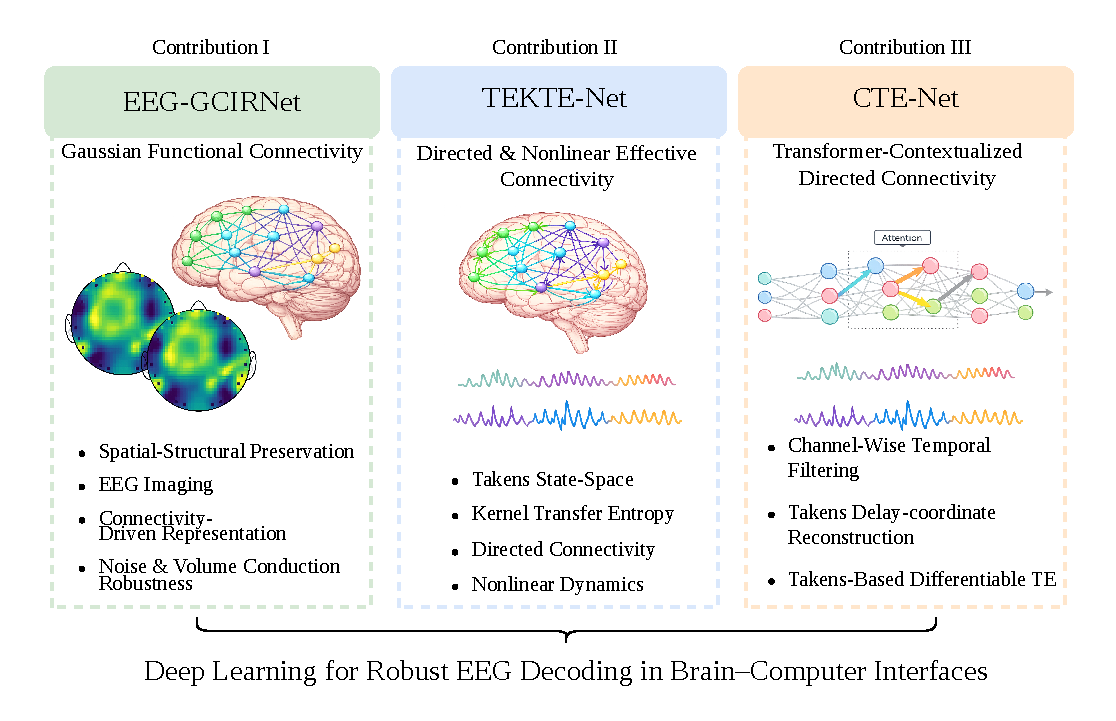
\includegraphics[width=\linewidth]{Figures/contributions.pdf}
    \caption{The three methodological contributions address robustness, interpretability, and generalization in \gls{eeg}-based \gls{bci} systems through connectivity-driven representations, nonlinear and directed predictive-dependency modeling, and Transformer-based contextualization.}
    \label{fig:contributions}
\end{figure}

This chapter presents a concise overview of the three methodological contributions developed in this doctoral thesis. The work is structured around methodological frameworks aimed at strengthening the robustness, interpretability, and generalization of \gls{eeg}-based \gls{bci} systems, considering the inherently noisy and highly variable nature of \gls{eeg} signals. The three contributions are grounded in peer-reviewed journal articles published by the author and are incorporated into a unified doctoral research framework in accordance with the intellectual property regulations of the Universidad Nacional de Colombia, available in the \href{https://unal.edu.co/archivos/user_upload/docs/legal.pdf}{Acuerdo 035 de 2003 del Consejo Académico}, and with the copyright and licensing policies of the respective publishers, including MDPI and Elsevier. An overview of the three contributions and their relationship with robustness, interpretability, and generalization is presented in Figure~\ref{fig:contributions}.

The first contribution, entitled \textbf{Gaussian Connectivity-Driven \gls{eeg} Imaging for Deep Learning-Based \gls{mi} Classification}, is based on the peer-reviewed article ``A Gaussian Connectivity-Driven EEG Imaging for Deep Learning-Based Motor Imagery Classification'' (Sensors, 2026). This contribution proposes a Gaussian connectivity-driven representation for constructing \gls{eeg} images that preserve spatial and structural relationships between channels. The proposed framework enables the integration of functional connectivity information within deep learning architectures, addressing limitations of traditional approaches based on local or channel-independent features and promoting improved discrimination of relevant neurophysiological patterns under conditions of noise, source mixing, and low spatial resolution.

The second contribution, entitled \textbf{Takens-Based Kernel \gls{te} Connectivity Network for \gls{mi} Classification}, is based on the peer-reviewed article ``Takens-Based Kernel Transfer Entropy Connectivity Network for Motor Imagery Classification'' (Sensors, 2025). This contribution extends the previous line of research by explicitly addressing nonlinear, directed, and time-dependent dependencies between \gls{eeg} signals. Through state-space reconstruction and kernel-based \gls{te} estimation, the proposed framework provides a richer characterization of directed predictive dependencies and dynamic information exchange between \gls{eeg} channels, capturing interactions that cannot be adequately represented by symmetric or static connectivity measures.

The third contribution, entitled \textbf{Transformer-Based Modeling of Directed Transfer Entropy Connectivity for EEG-Based ADHD Classification in Children}, is based on the peer-reviewed article ``Transformer-Based Modeling of Directed Transfer Entropy Connectivity for EEG-Based ADHD Classification in Children'' (Sensors, 2026). This contribution introduces CTE-Net, an end-to-end architecture that integrates Transformer-based contextualization, channel-wise nonlinear temporal filtering, Takens delay-coordinate reconstruction, and differentiable kernel-based \gls{te} estimation. The framework was developed to learn directed-connectivity representations from pediatric \gls{eeg} and was evaluated for the classification of children with \gls{adhd} and controls using subject-wise partitions and repeated training. In addition to predictive performance, this contribution examines the effects of the Transformer and \gls{te} components through ablation experiments and evaluates the organization, within-participant dispersion, and stability of the learned representations.

\subsection{Tested Datasets}\label{sec:datasets2}

To evaluate the effectiveness and robustness of the proposed methodology, extensive experiments were conducted using four \gls{eeg} datasets that are widely adopted in \gls{bci} research. Specifically, two binary \gls{mi} classification scenarios were considered using the \textit{GIGA MI} dataset and the \textit{BCI Competition IV 2a} dataset in their bi-class configurations. Additionally, the \textit{PhysioNet \gls{eeg} Motor Movement/Imagery} dataset was employed to address a multi-class \gls{mi} classification problem, allowing the assessment of the proposed approach under increased task complexity. Finally, the generalization capability of the methodology was evaluated on the \textit{\gls{eeg} data for \gls{adhd}/control children} dataset, which represents a clinical classification scenario aimed at distinguishing between children with \gls{adhd} and healthy control subjects.

\begin{itemize}
    \item[--] \textit{GIGAScience Dataset for \gls{eeg}-based \gls{mi}:} The GIGAScience \gls{mi} dataset, publicly available at \url{http://gigadb.org/dataset/100295} (accessed on 1 July 2025), provides one of the most comprehensive \gls{eeg} corpora for \gls{mi} analysis. The dataset comprises recordings from 52 healthy participants (50 with usable data), each performing a single \gls{eeg}-\gls{mi} session. Every session consists of five to six experimental blocks, with each block containing approximately 100–120 trials per class. Each trial spans seven seconds and follows a fixed timeline: an initial blank screen (0–2~s), a visual cue indicating either left- or right-hand \gls{mi} (2–5~s), and a concluding blank interval (5–7~s). Inter-trial intervals vary randomly between 0.1~s and 0.8~s to mitigate anticipatory bias, as illustrated in Figure~\ref{fig:giga_timeline}.

    \begin{figure}[htbp]
      \centering
      \input{Figures/GigaScience}
      \caption{Experimental timeline of the GigaScience \gls{mi}-\gls{eeg} dataset.}
      \label{fig:giga_timeline}
    \end{figure}    
    
    \gls{eeg} signals were recorded at a sampling frequency of 512~Hz using a 64-channel cap arranged according to the international 10--10 electrode placement system see Figure~\ref{fig:giga_montage}. In addition to the \gls{mi} sessions, the dataset includes recordings of real motor execution and six auxiliary non-task-related events—eye blinks, vertical and horizontal eye movements, head motions, jaw clenching, and resting state—enabling a broader exploration of \gls{eeg} noise sources and artifact correction. This multimodal composition makes the GigaScience particularly valuable for benchmarking advanced deep learning and connectivity-based \gls{eeg} decoding frameworks, as it supports both intra-subject and inter-subject generalization studies.

    \begin{figure}[htbp]
      \centering
      \resizebox{0.4\linewidth}{!}{\input{Figures/Giga}}
      \caption{Electrode montage, where colors indicate scalp regions:
      \protect\legend{frontal_left} Frontal left;
      \protect\legend{frontal} Frontal;
      \protect\legend{frontal_right} Frontal right;
      \protect\legend{central_left} Central left;
      \protect\legend{central_right} Central right;
      \protect\legend{posterior_left} Posterior left;
      \protect\legend{posterior} Posterior;
      \protect\legend{posterior_right} Posterior right.} 
      \label{fig:giga_montage}
    \end{figure}

    \item[--] \textit{\gls{bci} Competition IV dataset 2a:} a publicly available resource composed of \gls{eeg} recordings from nine healthy participants. These recordings were obtained during multiple trials of a (\gls{mi}) experiment with the protocol illustrated in~\Cref{fig:bci2a}. In each trial, participants first see a fixation cross on a computer screen, accompanied by an auditory cue. Two seconds later, a directional arrow appears for 1.25 seconds, signaling the start ($t=0$) of one of four possible \gls{mi} tasks: left-hand, right-hand, both feet, or tongue movement. One second after the \gls{mi} signal, subjects begin performing the instructed task during three seconds (i.e., until the 4-seconds mark after the instruction), at which point the cross disappears. A brief 1.5-second pause follows, during which the screen remains blank. For validation purposes, this study excludes feet and tongue movement tasks and focuses solely on binary classification of trials instructed to move the left ($y=0$) and right ($y=1$) hands. For each subject, the \gls{bci} Competition IV provides two subsets with the same experimental protocol: the training subset holds between 113 and 138 trials per subject, and the testing subset holds between 108 and 142 per subject~\cite{tangermann2012review}.
    
    \begin{figure}[htbp]
      \centering
      % Carga y escala al 90% del ancho de texto
      \resizebox{0.9\textwidth}{!}{\input{Figures/BCI2a.tex}}
      \caption{Schematic description of the \gls{mi} paradigms.}
      \label{fig:bci2a}
    \end{figure}

    The \gls{eeg} data were recorded using $C=22$ Ag/AgCl electrodes, placed according to the international 10/20 system as shown in~\Cref{fig:topoplot}. The data preprocessing applies a 50~Hz notch filter and a bandpass filter between 0.5 and 100~Hz and resamples to 250~Hz. Therefore, each participant comprises a subset of 22 channels and $N$ samples, and classification is based solely on labels 1 and 2, which distinguish between right-hand and left-hand \gls{mi}, respectively. Trials are split into two-seconds windows with 0.5 seconds overlap, that is $T=500$, from which the segments from 2.0 to 4.0 seconds after cue onset are selected to train the model as they are expected to hold the most relevant information to the \gls{mi} task. Lastly, the spherical splines method applies the surface Laplacian transform to each segment to reduce the influence of low spatial frequency activity, minimize the occurrence of spurious channel connectivities, and mitigate the volume conduction effect~\cite{tenke2015surface, hua2024scalp,lu2012adaptive, kapralov2024sensorimotor}.

    \begin{figure}[htbp]
      \centering
      
      \resizebox{0.5\textwidth}{!}{\input{Figures/electrodes}}
      \caption{Sensor positions according the 10--20 electrode placement system for the \gls{bci} Competition IV 2a dataset. 22 channels are distributed over ten main brain regions: \legend{frontal_left} Frontal left,\legend{frontal} Frontal,\legend{frontal_right} Frontal right,\legend{central_left} Central left,\legend{central_right} Central right,\legend{centro_parietal_left} Centro-parietal left,\legend{centro_parietal_right} Centro-parietal right,\legend{parietal_left} Parietal left,\legend{parietal_right} Parietal right,\legend{posterior} Posterior.}\label{fig:topoplot}
    \end{figure}
    
    \item[--] \textit{\gls{eeg} Motor Movement/Imagery Database:}The \gls{eegmmidb} \cite{physionet}, available at \url{https://physionet.org/content/eegmmidb/1.0.0/} (accessed on 7 December 2025), was employed as a secondary benchmark to evaluate the framework's versatility. This dataset comprises electroencephalographic recordings from 109 healthy participants performing a variety of real and imagined motor tasks. The \gls{eeg} signals were acquired using 64 scalp electrodes positioned according to the international 10--10 system see Figure~\ref{fig:giga_montage} and sampled at 160~Hz. The recording protocol encompasses 14 sessions per subject, including resting-state conditions, motor execution tasks, and \gls{mi} tasks. Data segmentation was performed based on event annotations to define discrete trials. Each trial corresponds to a 4.1~s window, yielding a raw input matrix of $64 \text{ channels} \times 640 \text{ samples}$. 
    
    To standardize the classification
    task, the original PhysioNet labels (0--11) were reorganized into five classes following a physiological interpretation of \gls{mi} tasks: (1) Left Hand \gls{mi} (labels 0 and 2); (2) Right Hand \gls{mi} (labels 1 and 3); (3) Both Fists \gls{mi} (labels 4 and 6); (4) Both Feet \gls{mi} (labels 5 and 7); and (5) Rest (label 11). Motor execution trials (label 10) and tongue \gls{mi} events (labels 8 and 9) were excluded from the analysis. In alignment with the experimental design of the GigaScience dataset, only \gls{mi}-related sessions and resting-state segments were considered. The experimental configuration is summarized in Figure~\ref{fig:physionet}.

    \begin{figure}[htbp]
     \centering
      % Paleta pastel alternativa
\definecolor{FixationColor}{HTML}{BFD8B8}
\definecolor{MotorColor}{HTML}{F6C28B}
\definecolor{RestColor}{HTML}{A7C5EB}
\definecolor{InterColor}{HTML}{EDE6F2}
\definecolor{CueColor}{HTML}{B5EAEA}

\begin{tikzpicture}
  % ===== Parámetros =====
  \def\boxheight{2.2}

  % Tiempos (s)
  \def\startRest{-2}
  \def\endRestA{0}
  \def\endMI{4.1}
  \def\endRestB{6.1}

  % ===== Bloques (SIN MARCOS) =====
  \fill[RestColor]  (\startRest,0) rectangle (\endRestA,\boxheight);
  \fill[MotorColor] (\endRestA,0)  rectangle (\endMI,\boxheight);
  \fill[RestColor]  (\endMI,0)     rectangle (\endRestB,\boxheight);

  % ===== Etiquetas internas =====
  \node[font=\small] at ({(\startRest+\endRestA)/2},{0.5*\boxheight}) {Rest};
  \node[font=\small] at ({(\endRestA+\endMI)/2},{0.5*\boxheight}) {Motor Imagery};
  \node[font=\small] at ({(\endMI+\endRestB)/2},{0.5*\boxheight}) {Rest};

  % ===== Eje X =====
  \draw[thick] (\startRest,0) -- (\endRestB,0)
        node[below right,font=\small] {Time [s]};

  \foreach \x/\lbl in {
      \startRest/-2,
      \endRestA/0,
      \endMI/4.1,
      \endRestB/6.1}{
    \draw (\x,0) -- ++(0,-2pt) node[below,font=\footnotesize] {\lbl};
  }

\end{tikzpicture}

      \caption{Overview of the \gls{eegmmidb} \gls{mi}-\gls{eeg} dataset: experimental timeline.}
      \label{fig:physionet}
    \end{figure}

    \item[--] \textit{\gls{adhd}/control children:}
    In this study, we use the publicly available \textit{\gls{eeg} data for \gls{adhd}/control children} dataset, collected and shared by Nasrabadi \textit{et al.} via IEEE DataPort~\cite{nasrabadi2020eeg}. The database comprises \gls{eeg} recordings from 121 school-aged children between 7 and 12 years old, including 61 diagnosed with \gls{adhd} and 60 typically developing control subjects~\cite{ekhlasi2021pte,li2025gcn}. \gls{adhd} diagnoses were established by an experienced child psychiatrist according to \gls{dsmiv} criteria. At the time of recording, patients had been treated with methylphenidate (Ritalin) for up to six months, whereas children in the control group had no history of psychiatric or neurological disorders, including epilepsy, or high-risk behaviors~\cite{ekhlasi2021pte,li2025gcn}.

    \begin{figure}[H]
      \centering
      \resizebox{0.5\textwidth}{!}{\input{Figures/TDHA Montage}}
     \caption{Scalp electrode montage following the international 10--20 system for the \gls{adhd}/control children dataset. The 19 \gls{eeg} channels are grouped into anatomically defined cortical regions, indicated by color: \legend{PurpleLeftSide} frontal left and central left, \legend{ElecBG} midline electrodes (Fz, Cz, Pz), \legend{Purple} frontal right, \legend{BlueRightSide} central right, \legend{GreenC} centro-parietal and parietal left, \legend{Orange} centro-parietal and parietal right, and \legend{UpperGreen} occipital region.}
    \label{fig:TDHA}
    \end{figure}
    
    \gls{eeg} signals were recorded while participants performed a visually guided attention task designed to probe attentional deficits associated with \gls{adhd}~\cite{ekhlasi2021pte,diagnosticInterface2024}. During the task, children were presented with a sequence of cartoon images containing a variable number of characters (ranging from 5 to 16 per image; see \Cref{fig:example}) and were instructed to silently count the number of Figures in each scene. Stimuli were displayed continuously, with each new image appearing immediately after the participant’s response, resulting in variable recording lengths depending on individual response times~\cite{li2025gcn,diagnosticInterface2024}.

    \begin{figure}[htbp]
    \centering
    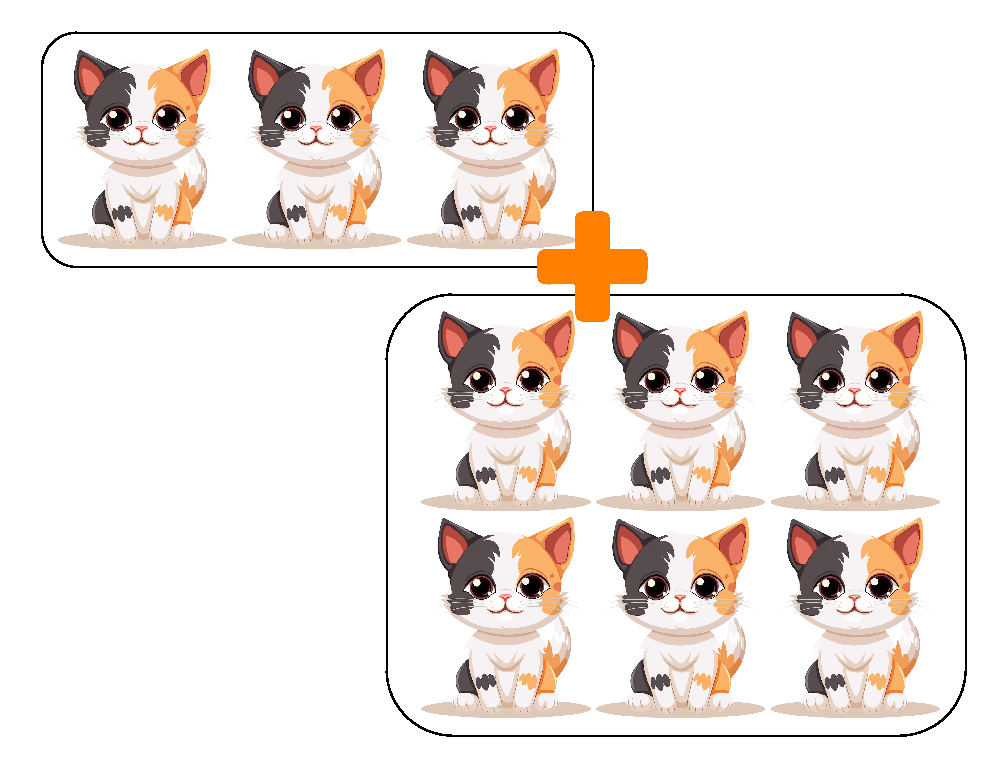
\includegraphics[width=0.7\linewidth]{Figures/TDHA.pdf}
    \caption{Example of the visual stimuli shown to
    children during \gls{eeg} recording.}
    \label{fig:example}
    \end{figure}

    \gls{eeg} recordings were acquired using 19 scalp electrodes placed according to the international 10--20 system (Fp1, Fp2, F3, F4, F7, F8, Fz, C3, C4, Cz, P3, P4, Pz, T3/T7, T4/T8, T5/P7, T6/P8, O1, O2; see \Cref{fig:TDHA}) at a sampling frequency of 128~Hz~\cite{nasrabadi2020eeg,diagnosticInterface2024,li2025gcn}. This dataset has been extensively used in effective connectivity studies based on Phase Transfer Entropy (\gls{pte}/\gls{dpte}) and multivariate \gls{te} to characterize altered directed information flow and short- and long-range connectivity patterns in \gls{adhd}~\cite{ekhlasi2021pte,ekhlasi2025omute,ekhlasi2021classification}.

    Following previous connectivity-based analyses, a standardized preprocessing pipeline was implemented using \gls{eeglab}~\cite{delorme2004eeglab,li2025gcn}. \gls{eeg} signals were re-referenced and calibrated to standard electrode coordinates, band-pass filtered between 0.5 and 60~Hz, and retained at a sampling frequency of 128~Hz. Artifacts related to eye blinks, muscle activity, and line noise were identified and removed using independent component analysis (\gls{ica}) combined with automatic component labeling (e.g., \gls{iclabel})~\cite{li2025gcn,delorme2004eeglab}. The cleaned continuous recordings were subsequently segmented into non-overlapping 5-s epochs, yielding a large set of artifact-free multi-channel segments for connectivity estimation and model training~\cite{li2025gcn,ekhlasi2021pte}.

    
\end{itemize}

%\chapter{\Objectiveonename}
\chapter[Gaussian Connectivity-Driven EEG Imaging for Deep Learning-Based Motor Imagery Classification]{Gaussian Connectivity-Driven EEG Imaging for Deep Learning-Based Motor Imagery Classification}
\chaptermark{EEG-GCIRNet}

{This contribution introduces} \gls{eeggcirnet}, a framework for MI classification built upon topographic maps derived from functional connectivity. The proposed methodology, illustrated in Figure~\ref{fig:EEGCIRNET}, comprises three primary stages: (i) preprocessing raw \gls{eeg} signals to compute GFC-based flow vectors; (ii) generating 2D topographic maps from these vectors; and (iii) processing the resulting images with a deep learning architecture for simultaneous classification and reconstruction.

%------------------------------------------------
 \begin{figure}[H]
  \centering
   \hspace{-25pt} 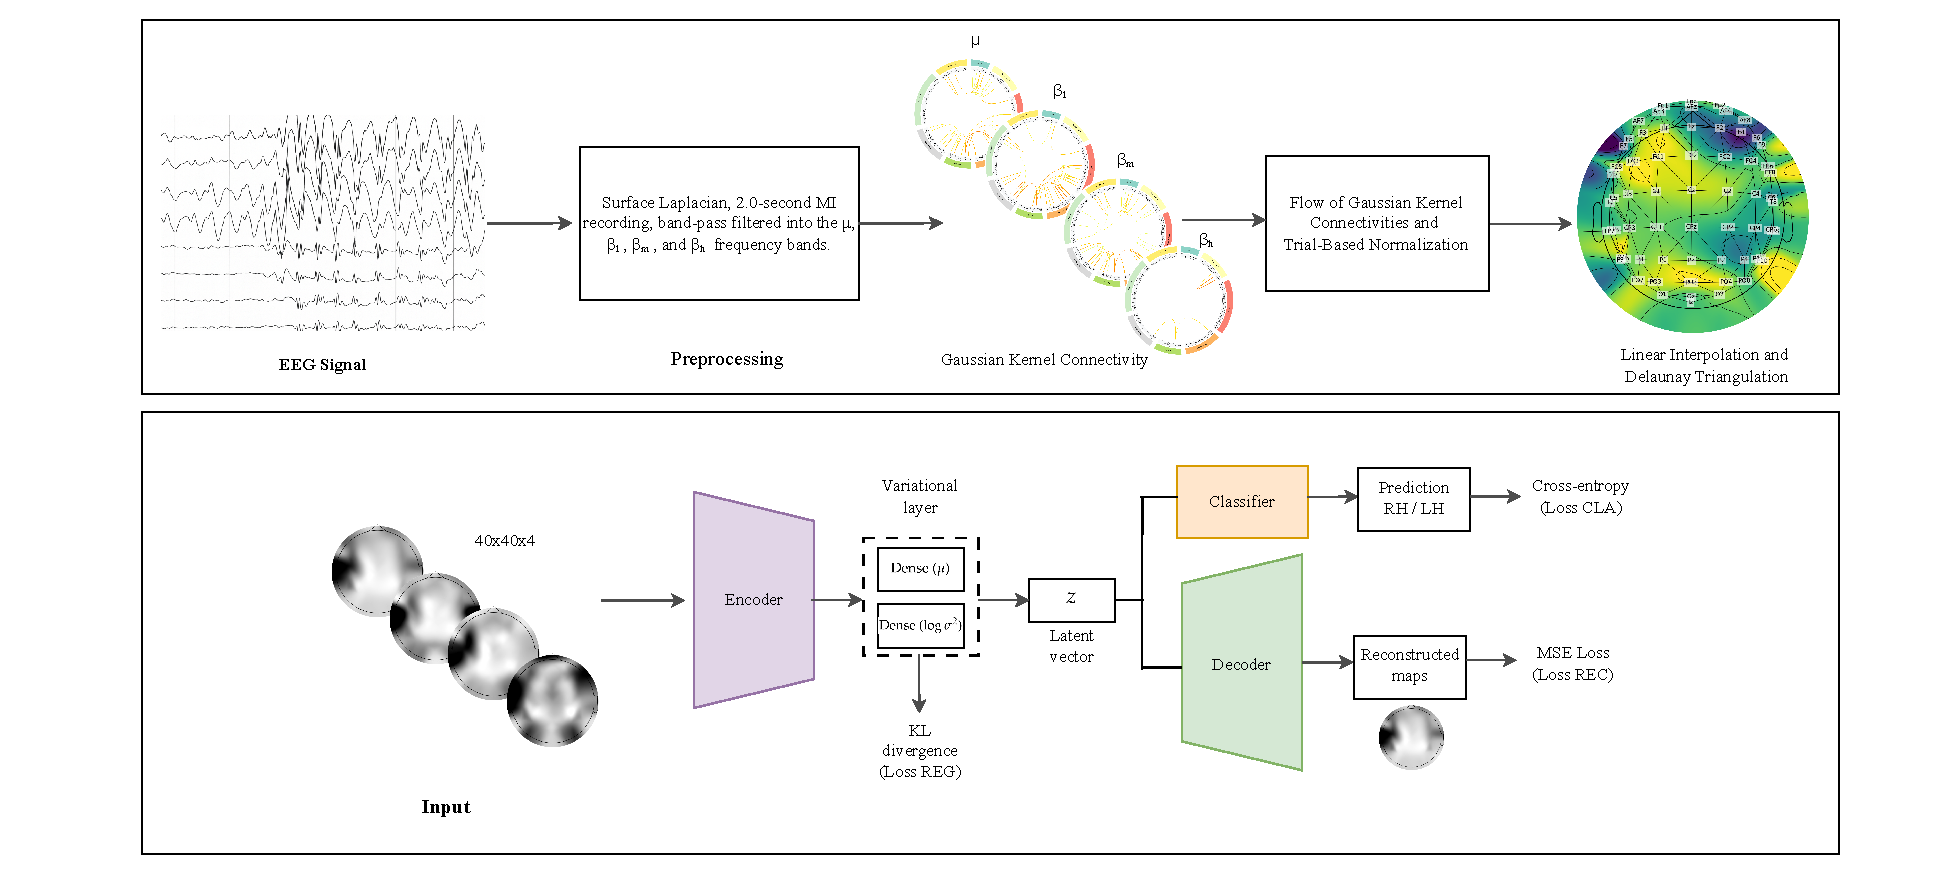
\includegraphics[width=\linewidth]{Figures/Scheme EEG-CIRNET.pdf}
    \caption{The
 proposed \gls{eeggcirnet} framework, composed of two main stages: (\textbf{Top}): A feature engineering pipeline that transforms raw \gls{eeg} signals into multi-channel topographic maps using GFC. {(\textbf{Bottom}):} A VAE architecture that processes these maps to jointly learn reconstruction, classification, and regularization from a shared latent space.}
    \label{fig:EEGCIRNET}
\end{figure}
%------------------------------------------------

% first preprocessing
\subsubsection{Stage 1: Signal Preprocessing and Feature Engineering}

First, an average reference was applied, which included the original reference electrode to ensure the data retained full rank. Subsequently, a fifth-order Butterworth bandpass filter was applied in the 4--40 Hz range. {To reduce computational load and maintain consistency across the evaluated deep learning models, the filtered signals of GigaScience and \gls{eegmmidb} dataset were resampled from 512 Hz and 160 Hz to 128 Hz, respectively~\cite{diagnostics13061122, computers12070145}. This study evaluates the proposed framework on two distinct experimental scenarios. First, for the GigaScience dataset, we focus on the binary classification of Left Hand versus Right Hand \gls{mi} ($Q=2$). This analysis was conducted on a subset of 50 subjects from the original cohort, with participants 29 and 34 excluded due to data availability constraints. Second, for the \gls{eegmmidb} database, the task is extended to the multi-class classification of five interpretable MI categories ($Q=5$). To ensure rigorous experimental consistency and following the experimental setup suggested in~\cite{bouchane2025hybrid}, a specific subset of ten subjects \{3, 7, 8, 9, 12, 13, 40, 41, 49, 50\} was selected, incorporating all valid trials associated with the target classes for these participants.}

Building upon this preprocessed data, the feature engineering process involves applying a Surface Laplacian filter to enhance the spatial resolution of the signals. {Specifically, the temporal segmentation was adapted to the recording protocol of each dataset. For the GigaScience repository, the data was segmented to isolate the active MI period, retaining the window from $2.5$ to $4.5$ s. In contrast, for the \gls{eegmmidb} collection, the entire trial duration of $4.1$ s was utilized.} The segmented data is further decomposed via band-pass filtering into four functionally distinct frequency bands: $\mu$ (8--12 Hz), low-beta ($\beta_l$, \mbox{12--15 Hz}), mid-beta ($\beta_m$, 15--20 Hz), and high-beta ($\beta_h$, 18--40 Hz). For each frequency band, GFC is computed to quantify the functional relationships between all channel pairs. The length scale hyperparameter $\sigma \in \mathbb{R}^+$, ruling the variance of the described data is adjusted to their median estimate as performed in~\cite{alvarez2014unsupervised}. The resulting connectivity information is then condensed into a normalized, channel-wise flow vector for each band. 

\subsubsection{Stage 2: Topographic Map Generation}

The second stage of the pipeline transforms the one-dimensional, GFC-based flow vectors into a two-dimensional, image-based representation suitable for processing with a CNN. This conversion is critical as it re-introduces the spatial topography of the \gls{eeg}electrodes, allowing the model to learn spatially coherent features.

This transformation was achieved via spatial interpolation, a process implemented using the visualization utilities within the MNE-Python library
 (\url{https://mne.tools/stable/index.html}, accessed on 1 June 2025). For each frequency band, the corresponding flow vector's values are mapped to the $2D$ coordinates of the \gls{eeg}electrodes. A mesh is then constructed over these coordinates using Delaunay triangulation. The pixel values for the final topographic map are subsequently estimated using linear barycentric interpolation within this mesh. This procedure is repeated for each of the four frequency bands ($\mu$, $\beta_l$, $\beta_m$, and $\beta_h$), yielding a set of four distinct topographic maps per trial. These maps are then stacked along the channel dimension to form a single, multi-channel image of size $40 \times 40 \times 4$. This resulting data structure serves as the final input to the \gls{eeggcirnet} architecture, providing a rich, spatio-spectral representation of the brain's functional connectivity during \gls{mi}.

\subsubsection{Stage 3: \gls{eeggcirnet} Architecture and Training}

%------------------------------------------
\begin{table}[H]%[h!]
\centering
\caption{Layer-wise configuration of the \gls{eeggcirnet} architecture. The input shape corresponds to the four-channel topographic maps ($\tilde{H} \times \tilde{W} \times C$).}
\label{tab:architecture}
\resizebox{\textwidth}{!}{%
\begin{tabular}{@{}llcccc@{}}
\toprule
\textbf{Block} & \textbf{Layer} & \textbf{Kernel/Units} & \textbf{Strides} & \textbf{Activation} & \textbf{Output Shape} \\ \midrule
\multicolumn{6}{c}{\textbf{Input Image}} \\
& & & & & $(40, 40, 4)$ \\ \midrule
\textbf{Encoder} & Conv2D & $3 \times 3$, 6 Filters & $(1, 1)$ & SELU & $(40, 40, 6)$ \\
($E_{\phi}$) & AvgPool2D & $2 \times 2$ & $(2, 2)$ & - & $(20, 20, 6)$ \\
& Conv2D & $3 \times 3$, 16 Filters & $(1, 1)$ & SELU & $(20, 20, 16)$ \\
& AvgPool2D & $2 \times 2$ & $(2, 2)$ & - & $(10, 10, 16)$ \\
& Conv2D & $3 \times 3$, 120 Filters & $(1, 1)$ & SELU & $(10, 10, 120)$ \\
& Flatten & - & - & - & $(12000)$ \\
& Dense & 128 Units & - & SELU & $(128)$ \\ \midrule
\textbf{Latent Space} & Dense ($\mu$) & 128 Units & - & Linear & $(128)$ \\
(Reparameterization) & Dense ($\log\sigma^2$) & 128 Units & - & Linear & $(128)$ \\ \midrule
\textbf{Decoder} & Dense & 128 Units & - & SELU & $(128)$ \\
($D_{\theta}$) & Dense & 12000 Units & - & SELU & $(12000)$ \\
& Reshape & $(10, 10, 120)$ & - & - & $(10, 10, 120)$ \\
& Conv2DTranspose & $3 \times 3$, 16 Filters & $(1, 1)$ & SELU & $(10, 10, 16)$ \\
& Upsampling & $2 \times 2$ & $(2, 2)$ & - & $(20, 20, 16)$ \\
& Conv2DTranspose & $3 \times 3$, 6 Filters & $(1, 1)$ & SELU & $(20, 20, 6)$ \\
& Upsampling & $2 \times 2$ & $(2, 2)$ & - & $(40, 40, 6)$ \\
& Reconstruction & $3 \times 3$ & - & Sigmoid & $(40, 40, 4)$ \\\midrule
\textbf{Classifier} & Dense & 128 Units & - & SELU & $(128)$ \\
($C_{\psi}$) & Dense (Output) & 2 Units & - & Softmax & $(2)$ \\ \bottomrule
\end{tabular}%
}
\end{table}
%------------------------------------------

The core of this model is a VAE with a convolutional architecture inspired by LeNet-5. This architecture is composed of three interconnected functional blocks operating on a shared latent space: an encoder, a decoder, and a classifier. 

The encoder block consists of two sequential pairs of convolutional and average pooling layers, which extract hierarchical spatial features from the input image. These features are then flattened and passed through a dense layer to produce a compact representation, which in turn parameterizes the mean ($\mu$) and log-variance ($\log\sigma^2$) vectors of the latent space. The decoder mirrors this structure using transposed convolutional layers to upsample the latent representation back to the original image dimensions. Concurrently, the classifier, a simple multi-layer perceptron, operates on the same latent vector to perform the final classification. The detailed layer-wise configuration of the \gls{eeggcirnet} is summarized in Table~\ref{tab:architecture}.

The \gls{eeggcirnet} model was trained end-to-end by optimizing the composite loss function described in Section~\ref{subsec:model}. The training was performed using the Adam optimizer with an initial learning rate of $1 \times 10^{-3}$. The hyperparameters that weight the loss components (i.e., $\lambda_{\text{REC}}$, $\lambda_{\text{CLA}}$, and $\lambda_{\text{REG}}$) were set using
 \texttt{KerasTuner} framework to ensure a balanced contribution from reconstruction, classification, and regularization objectives during training, subject to the constraint that they sum to one. The model was trained for a total of $200$ epochs with a batch size of $64$. An early stopping mechanism was employed with a patience of $10$ epochs, monitoring the validation loss to prevent overfitting and save the model with the best generalization performance. The model performance was evaluated using a subject-specific validation strategy. {For each of the considered subjects, we employed a \textit{Stratified} Shuffle Split
  cross-validation scheme with $5$ repetitions (\texttt{n\_splits=5}).} In each iteration, the trials were randomly partitioned into $80\%$ for training and $20\%$ for testing (\texttt{test\_size=0.2}), ensuring that the class distribution remained balanced in both sets. The results reported in this study correspond to the average accuracy obtained strictly on the {test sets} across these $5$ splits, ensuring that the reported metrics reflect the model's generalization capability on unseen data.

\section{Materials and Methods}

\subsubsection{Laplacian Filtering and Time Segmentation}\label{sec:laplacian}
% Laplacian filter
Each MI trial is structured for the proposed framework. Let $\{\mathbf{X} \in \mathbb{R}^{C \times \tau},\, \mathbf{y} \in \{0,1\}^Q\}$ denote a multichannel \gls{eeg}and its associated MI target label, where $\mathbf{X}$ represents the \gls{eeg} recording with $C$ spatial channels and $\tau$ temporal samples, and $\mathbf{y}$ is a one-hot encoded vector indicating the MI class among $Q$ possible categories.

To enhance the spatial resolution and mitigate the volume conduction effects inherent in \gls{eeg} recordings, a Surface Laplacian filter is applied to each trial $\mathbf{X} $. This filter acts as a spatial high-pass filter by estimating the second spatial derivative of the scalp potential at each electrode $c \in \mathcal{C}$ with respect to its neighbors $c' \in \mathcal{C}$, where $c \neq c'$. Following the methodology in~\cite{cohen2014analyzing}, this is achieved by using spherical splines to project the electrode positions onto a unit sphere, which allows for the interpolation of scalp potentials via Legendre polynomials. The interaction between any pair of electrodes $(c, c')$ is modeled as:
\begin{equation}
    p(c,c') = \frac{1}{4\pi} \sum_{n=1}^{N_{max}} \frac{\alpha (2n+1)P_n\left(\text{cosdist}(\mathbf{e}_c, \mathbf{e}_{c'})\right)}{(n(n+1))^{\rho - \alpha}},
    \label{eq:spline_interpolation}
\end{equation}
%
where $P_n$ is the Legendre Polynomial of order $n$, $N_{max}$ is the highest polynomial order considered, $\rho \in \mathbb{R}^{+}$ is a smoothness constant, and $\mathbf{e}_c, \mathbf{e}_{c'} \in \mathbb{R}^3$ are the 3D electrode positions normalized to a unit-radius sphere. The cosine distance is defined as $\text{cosdist}(\mathbf{e}_c, \mathbf{e}_{c'}) = 1 - \|\mathbf{e}_c - \mathbf{e}_{c'}\|_2 / 2$.

The Laplacian-filtered \gls{eeg} data, denoted as $\mathbf{X_L} \in \mathbb{R}^{C \times \tau}$, is subsequently computed using the weighting matrices derived from the spline interpolation:
%
\begin{equation}
    \mathbf{X_L} = \mathbf{H}\left(\mathbf{X}^{\top}\mathbf{G}_{s}^{-1} - \mathbf{X}^{\top}\mathbf{G}_{s}^{-1}\mathbf{1}\mathbf{G}_{s}^{-1}/\mathbf{1}^{\top}\mathbf{G}_{s}^{-1}\mathbf{1}\right)^{\top},
    \label{eq:laplacian_filter}
\end{equation}
%
where $\mathbf{1} \in \mathbb{R}^{C}$ is a column vector of ones, $\mathbf{I} \in \mathbb{R}^{C \times C}$ is the identity matrix, and $\lambda \in [0, 1]$ is a regularization parameter. The matrix $\mathbf{G}_s = \mathbf{G} + \lambda\mathbf{I}$ is a regularized (smoothed) version of $\mathbf{G}$. The weighting matrices $\mathbf{G}, \mathbf{H} \in \mathbb{R}^{C \times C}$ hold the elements derived from Equation~\eqref{eq:spline_interpolation}, with their specific values determined by the parameter $\alpha$ as follows:
%
\begin{equation}
    \alpha = 
    \begin{cases} 
        1, & \text{where } p(c,c') = g(c,c') \\ 
        -1, & \text{where } p(c,c') = h(c,c') 
    \end{cases},
\end{equation}
%
where $g(c,c')$ and $h(c,c')$ are the elements of matrices $\mathbf{G}$ and $\mathbf{H}$, respectively. This filtering step produces a spatially enhanced representation $\mathbf{X_L}$ that serves as input for the subsequent feature extraction stages.

% Time segmentation
Further, to focus the analysis exclusively on the period of active \gls{mi}, the Laplacian-filtered signal $\mathbf{X_L}$ is temporally segmented. The time window corresponding to the MI task, specifically between $t_s$ and $t_e$ seconds of each trial, is retained. Let $t_s$ and $t_e$ be the start and end times of the MI segment, and $f_s$ be the sampling frequency, the segmented signal $\mathbf{X}_{seg} \in \mathbb{R}^{C \times \tau}$ is obtained as:
%
\begin{equation}
    \mathbf{X}_{seg} = \mathbf{X_L}[:, t_s \cdot f_s : t_e \cdot f_s],
    \label{eq:segmentation}
\end{equation}
%
where the slicing notation $[t_s \cdot f_s : t_e \cdot f_s]$ indicates the selection of temporal samples from the start index to the end index. For brevity, this segmented signal will be denoted as $\mathbf{X}$ in the subsequent sections.

\subsubsection{Kernel-Based Cross-Spectral Gaussian Connectivity for \gls{eeg} Imaging}\label{sec:kcs}

%input-output
To model the mutual dependency between \gls{eeg} channels, we consider any two channels \( \mathbf{x}_c, \mathbf{x}_{c'} \in \mathbb{R}^\tau \) from a given trial $\mathbf{X}$ (where $c,c'\in C$). Their mutual dependency can be captured using a stationary kernel \( \kappa : \mathbb{R}^\tau \times \mathbb{R}^\tau \rightarrow \mathbb{R} \), which maps both signals into a reproducing kernel Hilbert space (RKHS) via a nonlinear feature map \( \phi : \mathbb{R}^\tau \rightarrow \mathcal{H} \)~\cite{kanagawa2018gaussianprocesseskernelmethods}. Indeed, according to Bochner’s theorem, a sufficient condition for the kernel $\kappa$ to be stationary is that it admits a spectral representation~\cite{JMLR:v25:22-1434}:
\begin{equation}
\kappa(\mathbf{x}_c - \mathbf{x}_{c'}) = \int_{{\Omega_b}} \exp\left( j2\pi (\mathbf{x}_c - \mathbf{x}_{c'})^\top \mathbf{f} \right) S_{\mathbf{x}_c\mathbf{x}_{c'}}(\mathbf{f})\, d\mathbf{f},
\label{eq:stationary_kernel}
\end{equation}
where \( \mathbf{f} \in \boldsymbol{\Omega} \subseteq \mathbb{R}^\tau \) is a frequency vector, and \( S_{\mathbf{x}_c\mathbf{x}_{c'}}(\mathbf{f}) = \frac{dP_{\mathbf{x}_c\mathbf{x}_{c'}}(\mathbf{f})}{d\mathbf{f}} \in \mathbb{C} \) is the cross-spectral density between \( \mathbf{x} \) and \( \mathbf{x}' \), derived from the spectral distribution \( P_{\mathbf{x}_c\mathbf{x}_{c'}}(\mathbf{f}) \).

Building on this spectral representation, the cross-spectral power within a specific frequency band $\Omega_b$ can be computed via the Fourier transform of the kernel:
\begin{equation}
P_{\mathbf{x}_c\mathbf{x}_{c'}}({\Omega_b}) = 2 \int_{{\Omega_b}} \mathcal{F}\left\{ \kappa(\mathbf{x}_c - \mathbf{x}_{c'}) \right\} d\mathbf{f},
\label{eq:cross_spectral_band}
\end{equation}
where \( \mathcal{F}\{\cdot\} \) denotes the Fourier transform. This spectral formulation allows capturing both linear and nonlinear dependencies in the frequency domain, making it particularly useful for analyzing brain signals.

A widely used choice for \( \kappa \) is the Gaussian kernel, which ensures smoothness, locality, and analytic tractability~\cite{rasmussen2006gaussian}:
\begin{equation}
\kappa_G(\mathbf{x}_c - \mathbf{x}_{c'}; \sigma) = \exp\left( -\frac{\|\mathbf{x}_c - \mathbf{x}_{c'}\|_2^2}{2\sigma^2} \right),
\end{equation}
where \( \sigma \in \mathbb{R}^+ \) is a bandwidth hyper-parameter.

%filter bank
Inspired by the kernel-based spectral approaches introduced in~\cite{diagnostics13061122}, we compute a Gaussian kernel cross-spectral connectivity estimator to encode spatio--frequency interactions among pairwise \gls{eeg} channels. Specifically, for each \gls{eeg} channel \( c \), a band-limited spectral reconstruction is obtained as:
\begin{equation}\label{eq:fbank}
\mathbf{x}_c^{({\Omega_b})} = 
\mathcal{F}^{-1}\left\{\mathcal{F}\{\mathbf{x}_c\}; {\Omega_b}\right\},
\end{equation}
where \( {\Omega_b} \) denotes a given frequency bandwidth (rhythm). 
Then, the Gaussian Function Connectivity (GFC) matrix 
\( \mathbf{K}^{({\Omega_b})} \in [0,1]^{C\times C} \) is derived to quantify 
the degree of similarity between the spectral representations of all channel pairs, as:
\begin{equation}
K^{({\Omega_b})}_{cc'} = 
\kappa_G\left(\mathbf{x}^{({\Omega_b})}_c - \mathbf{x}^{({\Omega_b})}_{c'}; 
\sigma_{{\Omega_b}}\right),
\label{eq:gfc}
\end{equation}
where \( \kappa_G(\cdot; \sigma_{{\Omega_b}}) \) is a Gaussian kernel with scale parameter \( \sigma_{{\Omega_b}} \). To ensure adaptive sensitivity across rhythms, \( \sigma_{{\Omega_b}} \) is estimated as the 
median of all pairwise Euclidean distances between spectral reconstructions 
\( \mathbf{x}^{({\Omega_b})}_c \) and \( \mathbf{x}^{({\Omega_b})}_{c'} \), \( \forall\, c,c'\in C \). This formulation provides a data-driven normalization of connectivity strength, enabling robust comparison across heterogeneous \gls{eeg} rhythms and subjects.

%GFC flow
Afterward, we propose to compute an \gls{eeg} connectivity flow from 
\(\mathbf{K}^{({\Omega_b})}\), preserving a direct one-to-one correspondence 
with the electrode spatial configuration. Specifically, the GFC flow vector \(\mathbf{g}^{({\Omega_b})} \in [0,1]^C\) holds elements:
\begin{equation}\label{eq:flowGFC}
g_c^{({\Omega_b})} = 
\frac{1}{C} \sum_{\substack{c'=1 \\ c' \neq c}}^{C} 
K^{({\Omega_b})}_{cc'},
\end{equation}
where each element \( g_c^{({\Omega_b})} \) represents the mean functional coupling of channel \( c \) with all other channels within the given frequency band \({\Omega_b} \). The latter compresses the pairwise connectivity information into a compact, channel-wise flow representation while retaining the spatial and spectral data patterns.

To ensure a consistent feature scale for the imaging stage, the GFC flow vectors are normalized across the entire training dataset. Specifically, a channel-wise Min-Max normalization is applied, scaling the connectivity values of each channel to a uniform range of $[0, 1]$. This procedure preserves the relative topography of neural connectivity while standardizing the input scale, yielding the normalized flow vector $\tilde{\mathbf{g}}^{(\Omega_b)}$ for each trial.

\subsubsection{Topographic Map Generation}

%topographic interpolation
The final feature engineering step transforms the one-dimensional GFC flow vectors into two-dimensional topographic images, creating a data representation suitable for convolutional neural network (CNN) architectures. For each trial, this process converts the normalized flow vector $\tilde{\mathbf{g}}^{(\Omega_b)} \in [0, 1]^C$ from each frequency band into a corresponding topographic image $\mathbf{T}^{(\Omega_b)} \in \mathbb{R}^{\tilde{H} \times \tilde{W}}$.

This transformation is accomplished via spatial interpolation guided by Delaunay triangulation. First, the set of 2D scalp coordinates of the electrodes, $P = \{(x_c, y_c)\}_{c=1}^C$, is triangulated. This partitions the electrode layout into a mesh of non-overlapping triangles, where the circumcircle of each triangle contains no other electrode points. This triangulation provides a structured grid for interpolating the connectivity values, where each element $\tilde{g}_c^{(\Omega_b)}$ is associated with its corresponding coordinate $(x_c, y_c)$.

To generate the final image, the value $V(x, y)$ for each pixel is computed using barycentric interpolation within its enclosing triangle $T_k = (p_1, p_2, p_3)$:
%
\begin{equation}
    V(x, y) = \lambda_1(x, y) v(p_1) + \lambda_2(x, y) v(p_2) + \lambda_3(x, y) v(p_3),
    \label{eq:barycentric_interpolation}
\end{equation}
%
where $v(p_i)$ is the connectivity value at vertex $p_i$, and $\lambda_1, \lambda_2, \lambda_3$ are the barycentric coordinates of $(x, y)$ satisfying $\sum_{j=1}^{3} \lambda_j = 1$ and $\lambda_j \geq 0$. This procedure is applied across all pixels to render the smooth topographic map $\mathbf{T}^{(\Omega_b)}$. The resulting set of four maps (one for each frequency band) is then stacked to form a multi-channel image, which serves as the final input to the deep learning model.


\subsubsection{\gls{eeggcirnet}: Multimodal Architecture}\label{subsec:model}

The proposed model is a variational autoencoder (VAE) designed to process topographic maps derived from functional connectivity representations. Its architecture relies on a single input stream that learns to extract and encode the most relevant spatial features from the maps, which are then projected into a shared latent space where a multivariate Gaussian distribution is modeled. From this latent space, the model simultaneously performs reconstruction of the topographic maps and classification of \gls{mi} tasks. These objectives are integrated within a composite loss function that balances reconstruction fidelity, classification accuracy, and latent space regularization. This approach enables the learning of robust and interpretable latent representations capable of capturing discriminative spatial relationships and adapting to the variability and noise inherent in \mbox{\gls{eeg} signals.}

The core of our framework is a VAE based on the LeNet-5 architecture, which is partitioned into three functional blocks: an encoder, a decoder, and a classifier, all operating on the shared latent space. Let $Y \in \mathbb{R}^{\tilde{H} \times \tilde{W} \times B}$ be the multi-channel input image for a given trial, formed by stacking the $B$ topographic maps (one for each frequency band).

The encoder, defined as a function $E_{\phi}$ parameterized by $\phi$, maps the input image $Y$ to the parameters of the posterior distribution $q_{\phi}(z|Y)$. This transformation is realized through a composition of functions, where each function represents a layer in the network:
\begin{equation}
    h_E = (f_5 \circ f_4 \circ f_3 \circ f_2 \circ f_1)(Y)
\end{equation}

Here, $f_1$ and $f_3$ are convolutional layers with {SELU} activation, $f_2$ and $f_4$ are average pooling layers, and $f_5$ is a fully connected layer with {SELU} activation after flattening the feature maps. The resulting hidden representation $h_E$ is then linearly transformed to produce the mean vector $\mu$ and the log-variance vector $\log \sigma^2$ of the latent space:
\begin{align}
    \mu &= W_{\mu}h_E + b_{\mu} \\
    \log \sigma^2 &= W_{\sigma}h_E + b_{\sigma}
\end{align}

The decoder, defined as a function $D_{\theta}$ parameterized by $\theta$, reconstructs the original input image $\hat{Y}$ from a latent vector $z \sim q_{\phi}(z|Y)$. Its architecture mirrors the encoder by composing functions that progressively up-sample the representation to the original \mbox{image dimensions:}
\begin{equation}
    \hat{Y} = (g_3 \circ g_2 \circ g_1)(z)
\end{equation}

Here,
$g_1$ is a fully connected layer followed by a reshape operation, $g_2$ is a transposed convolutional layer with {SELU} activation, and $g_3$ is a final transposed convolutional layer with a Sigmoid activation to ensure the output pixel values are in a normalized range.

Concurrently, the classifier, a function $C_{\psi}$ parameterized by $\psi$, predicts the MI task label probabilities $\hat{p}$ from the same latent vector $z$. It is implemented as a multi-layer perceptron:
\begin{equation}
    \hat{p} = C_{\psi}(z) = \text{Softmax}(W_c( \text{SELU}(W_h z + b_h)) + b_c)
\end{equation}

Formally, the latent vector $z_i$ for a given input sample $i$ is computed using the reparameterization trick:
\begin{equation}
    z_i = \mu_i + \exp\left(\frac{1}{2}\log\sigma_i^2\right) \odot \epsilon_i, \quad \epsilon_i \sim \mathcal{N}(0, I)
\end{equation}
where $\mu_i$ and $\sigma_i^2$ denote the mean and variance of the approximate posterior distribution learned by the encoder for sample $i$, and $\epsilon_i$ is drawn from a standard normal distribution. The exponential term ensures the sampled standard deviation remains strictly positive.

The total objective function, $\mathcal{L}_{\text{total}}$, is defined as a weighted sum of the three loss terms:
\begin{align}
\mathcal{L}_{\text{total}} = \ & \lambda_{\text{REC}} \cdot \mathcal{L}_{\text{REC}} + \lambda_{\text{CLA}} \cdot \mathcal{L}_{\text{CLA}} + \lambda_{\text{REG}} \cdot \mathcal{L}_{\text{REG}} \\
\intertext{where}
\mathcal{L}_{\text{REC}} &= \frac{ \frac{1}{N} \sum_{i=1}^{N} \lVert Y_i - \hat{Y}_i \rVert_F^2 }{ \frac{1}{N} \sum_{i=1}^{N} \lVert Y_i - \bar{Y} \rVert_F^2 } \label{eq:rec} \\
\mathcal{L}_{\text{CLA}} &= \frac{1}{N} \sum_{i=1}^{N} \frac{ \mathcal{L}_{\mathrm{cce}}(p_i, \hat{p}_i) }{ \mathcal{L}_{\mathrm{cce}}([0.5, 0.5], \hat{p}_i)} \label{eq:cla} \\
\mathcal{L}_{\text{REG}} &= \frac{1}{N \log N} \sum_{i=1}^{N} D_{\text{KL}}(q_{\phi}(z_i|Y_i) || \mathcal{N}(0, I)) \label{eq:reg}
\end{align}

\noindent
where $\lambda_{\text{REC}}$, $\lambda_{\text{CLA}}$, and $\lambda_{\text{REG}}$ are hyperparameters controlling the contribution of each term.
The first component, $\mathcal{L}_{\text{REC}}$, is the normalized mean squared error (NMSE), which evaluates reconstruction accuracy by comparing the original topographic maps ($Y_i$) and their reconstructions ($\hat{Y}_i$), normalized by the dataset's variance ($\bar{Y}$ is the mean image). The Frobenius norm, $\lVert \cdot \rVert_F$, is used for the image-wise error.
The second term, $\mathcal{L}_{\text{CLA}}$, represents the normalized binary cross-entropy (NBCE). It penalizes misclassifications between the true one-hot labels ($p_i$) and predicted probabilities ($\hat{p}_i$), while adjusting the loss based on the entropy over an ideal, non-informative prediction (e.g., a uniform distribution $[0.5, 0.5]$). This maintains a balanced contribution from all classes.
Finally, the third term, $\mathcal{L}_{\text{REG}}$, is the normalized Kullback–Leibler (KL) divergence between the approximate posterior $q_{\phi}(z_i|Y_i)$ and a unit Gaussian prior $\mathcal{N}(0, I)$. This regularizes the latent space, promoting smoothness and disentanglement in the learned representations.

This KL divergence term encourages the latent representations to follow a standard normal distribution, promoting structure and generalization. The use of $\log N$ in the denominator prevents this term from dominating the loss in large batches. Taken together, these components ensure that the model jointly optimizes for faithful reconstruction, discriminative performance, and a well-regularized latent structure—crucial for interpretable and generalizable multimodal brain–computer interfaces.

The model is trained by solving the following optimization problem:
\[
\{\phi^*, \theta^*, \psi^*\} = \arg\min_{\phi, \theta, \psi} \mathcal{L}_{\text{total}}
\]
where $\{\phi, \theta, \psi\}$ denotes the complete set of trainable parameters in the encoder, decoder, and classifier, respectively.



\subsubsection{Evaluation Criteria}

The performance of the proposed \gls{eeggcirnet} was rigorously evaluated using a multi-faceted approach tailored to the specific requirements of each experimental scenario. For the GigaScience dataset ($Q=2$), the primary quantitative metric was subject-specific binary classification accuracy, benchmarked against seven baseline and state-of-the-art models. For the \gls{eegmmidb} dataset, the evaluation was extended to a multi-class setting ($Q=5$), focusing on the model's ability to resolve complex decision boundaries across five distinct \gls{mi} categories.

To validate the findings, a robust statistical framework was employed. A Friedman test was used to assess overall significance across models, followed by post-hoc pairwise $t$-tests for direct comparisons. To account for the multiple comparisons problem, the resulting $p$-values were adjusted using the \textit{Holm-Bonferroni} correction method to control the family-wise error rate. Furthermore, the framework's robustness and generalization capabilities were analyzed by stratifying the GigaScience cohort into ``Good'' (accuracy $> 80\%$), ``Mid'' (accuracy $60\%$--$80\%$), and ``Bad'' (accuracy $< 60\%$) performance groups based on the standard EEGNet baseline. This stratification allowed for a targeted assessment of the model's corrective effectiveness across varying \gls{eeg}signal qualities.

Beyond quantitative metrics, the evaluation delved into the model's interpretability by leveraging its variational autoencoder architecture and gradient-based analysis. This qualitative assessment involved three key methods: \textit{(i)} a visual analysis of the reconstructed topographic maps to confirm that the model learned physiologically relevant spatio-spectral patterns; \textit{(ii)} the visualization of the latent space using t-SNE projections to directly inspect the quality of class separability and feature disentanglement; and \textit{(iii)}~a layer-wise relevance analysis using Grad-CAM++. The latter was employed to verify that the model's decision-making is driven by spatial contributions from neurophysiologically valid regions---such as the sensorimotor cortex---rather than artifacts. This combined quantitative and qualitative evaluation provides a holistic validation of the \gls{eeggcirnet} framework, covering its accuracy, statistical significance, and the meaningfulness of its learned internal representations.

\subsection{Results}\label{sec:Results}
%------------------------------------------------

\subsubsection{Binary MI Classification Performance on the GigaScience Database}
%------------------------------------------------
\begin{figure}[H]
  %----- PALETA (Tableau-like)
\definecolor{modelBlue}{RGB}{31,119,180}   % EEGNet
\definecolor{modelOrange}{RGB}{255,127,14} % KREEGNet
\definecolor{modelGreen}{RGB}{44,160,44}   % KCS-FCNet
\definecolor{modelRed}{RGB}{214,39,40}     % DeepConvNet
\definecolor{modelPurple}{RGB}{148,103,189}% ShallowConvNet
\definecolor{modelBrown}{RGB}{140,86,75}   % TCFusionNet
\definecolor{modelGray}{RGB}{127,127,127}  % CSP
\definecolor{modelOlive}{RGB}{188,189,34}  % \gls{eeggcirnet} (NRVAE)

%----- ESTILOS (sin markers globalmente)
\pgfplotsset{
  every axis plot/.style={solid, mark=none}, % <-- sin marcadores
  myaxis/.style={
    width=0.9\linewidth,
    height=0.16\paperheight,
    scale only axis,
    ymin=0.40, ymax=1.00,
    xtick pos=bottom,
    ytick pos=left,
    tick align=inside,
    ytick={0.40,0.50,0.60,0.70,0.80,0.90,1.00},
    yticklabels={40,50,60,70,80,90,100},
    ylabel={Accuracy (\%)},
    xlabel={Subjects},
    xmin=-0.5, xmax=49.5,   % datos x = 0..49
    xtick=data,
    xticklabel style={rotate=90, anchor=east, font=\scriptsize},
    yticklabel style={font=\scriptsize},
    label style={font=\small},
    axis lines=box,
    xmajorgrids, ymajorgrids,
    grid style={black!15},
    legend style={
  at={(0.004,0.35)}, anchor=north west, % esquina sup. izquierda del recuadro de la gráfica
  draw=black!25, fill=white, fill opacity=0.8, text opacity=1,
  font=\scriptsize,                
  inner sep=0.4pt,            
  row sep=0.4pt, column sep=1pt 
},
legend image post style={xscale=0.3},
legend cell align=left,
legend columns=2, 
  }
}

\begin{tikzpicture}
\begin{axis}[myaxis,
  xticklabels={43,14,3,50,48,4,35,13,23,41,1,49,37,26,5,44,6,47,28,36,12,39,46,10,20,22,31,18,52,25,21,40,24,27,30,51,42,9,16,38,11,19,33,2,17,15,45,32,7,8}
]

  %----- Bandas de fondo (0.40–0.60 rojo, 0.60–0.80 amarillo, 0.80–1.00 verde)
  \path[fill=red!40,    opacity=0.40] (axis cs:-0.5,0.40) rectangle (axis cs:49.5,0.60);
  \path[fill=yellow!50, opacity=0.40] (axis cs:-0.5,0.60) rectangle (axis cs:49.5,0.80);
  \path[fill=green!40,  opacity=0.40] (axis cs:-0.5,0.80) rectangle (axis cs:49.5,1.00);

  %----- Curvas (sin markers)
  \addplot[line width=0.9pt, color=modelBlue]
     coordinates {(0,0.99500) (1,0.97000) (2,0.93500) (3,0.92500) (4,0.92500) (5,0.91000) (6,0.88000) (7,0.84000) (8,0.84000) (9,0.83000) (10,0.81000) (11,0.78970) (12,0.77000) (13,0.76500) (14,0.76500) (15,0.76000) (16,0.75560) (17,0.74870) (18,0.74500) (19,0.73850) (20,0.72570) (21,0.71000) (22,0.69170) (23,0.68000) (24,0.64710) (25,0.64000) (26,0.63000) (27,0.62000) (28,0.61500) (29,0.60500) (30,0.59000) (31,0.58000) (32,0.57500) (33,0.56220) (34,0.56000) (35,0.55900) (36,0.55500) (37,0.55000) (38,0.55000) (39,0.54870) (40,0.54500) (41,0.54480) (42,0.54000) (43,0.54000) (44,0.53500) (45,0.53330) (46,0.53000) (47,0.52000) (48,0.51670) (49,0.50000)};
  \addlegendentry{EEGNet}

  \addplot[line width=0.9pt, color=modelOrange]
    coordinates {(0,0.98500) (1,0.97500) (2,0.98000) (3,0.97000) (4,0.96500) (5,0.96000) (6,0.87000) (7,0.94000) (8,0.93000) (9,0.94500) (10,0.88500) (11,0.83080) (12,0.84500) (13,0.89500) (14,0.88500) (15,0.90000) (16,0.85000) (17,0.81540) (18,0.83500) (19,0.74870) (20,0.79430) (21,0.78500) (22,0.80420) (23,0.85000) (24,0.74120) (25,0.77000) (26,0.79000) (27,0.73500) (28,0.69500) (29,0.85500) (30,0.82500) (31,0.58500) (32,0.76000) (33,0.58920) (34,0.61600) (35,0.61540) (36,0.70500) (37,0.68750) (38,0.56500) (39,0.54870) (40,0.64000) (41,0.64140) (42,0.58000) (43,0.54500) (44,0.58500) (45,0.88210) (46,0.64500) (47,0.58000) (48,0.60000) (49,0.63500)};
  \addlegendentry{KREEGNet}

  \addplot[line width=0.9pt, color=modelGreen]
    coordinates {(0,0.96500) (1,0.96000) (2,0.92500) (3,0.85500) (4,0.90500) (5,0.91500) (6,0.82000) (7,0.80000) (8,0.88500) (9,0.87500) (10,0.73500) (11,0.83590) (12,0.79000) (13,0.79500) (14,0.81000) (15,0.83000) (16,0.77780) (17,0.69740) (18,0.74000) (19,0.70770) (20,0.69140) (21,0.77500) (22,0.78330) (23,0.75000) (24,0.72940) (25,0.68000) (26,0.84000) (27,0.76000) (28,0.73000) (29,0.65000) (30,0.76500) (31,0.64000) (32,0.72000) (33,0.46490) (34,0.69600) (35,0.51790) (36,0.77000) (37,0.71250) (38,0.48000) (39,0.54360) (40,0.52000) (41,0.62070) (42,0.62500) (43,0.56000) (44,0.54000) (45,0.80000) (46,0.61000) (47,0.60000) (48,0.61670) (49,0.57000)};
  \addlegendentry{KCS-FCNet}

  \addplot[line width=0.9pt, color=modelRed]
    coordinates {(0,0.98500) (1,0.95000) (2,0.81500) (3,0.86500) (4,0.79500) (5,0.80000) (6,0.85000) (7,0.90000) (8,0.72500) (9,0.65000) (10,0.78500) (11,0.72310) (12,0.80500) (13,0.78500) (14,0.67500) (15,0.87500) (16,0.73330) (17,0.77440) (18,0.69000) (19,0.69230) (20,0.66290) (21,0.75500) (22,0.75830) (23,0.61000) (24,0.71760) (25,0.61500) (26,0.54500) (27,0.62500) (28,0.52500) (29,0.60000) (30,0.59000) (31,0.54500) (32,0.63000) (33,0.54590) (34,0.52800) (35,0.58970) (36,0.55000) (37,0.57080) (38,0.54000) (39,0.53850) (40,0.49000) (41,0.50340) (42,0.55500) (43,0.53500) (44,0.53500) (45,0.50260) (46,0.55500) (47,0.55500) (48,0.56670) (49,0.56000)};
  \addlegendentry{DeepConvNet}

  \addplot[line width=0.9pt, color=modelPurple]
    coordinates {(0,0.98000) (1,0.96500) (2,0.96000) (3,0.96000) (4,0.94500) (5,0.93500) (6,0.86500) (7,0.90500) (8,0.87500) (9,0.92500) (10,0.89500) (11,0.86670) (12,0.85500) (13,0.86500) (14,0.91000) (15,0.92000) (16,0.83330) (17,0.83080) (18,0.75000) (19,0.70770) (20,0.73710) (21,0.79000) (22,0.80420) (23,0.75000) (24,0.71760) (25,0.69500) (26,0.74000) (27,0.62000) (28,0.70500) (29,0.68500) (30,0.58500) (31,0.61500) (32,0.75000) (33,0.60540) (34,0.58400) (35,0.55380) (36,0.62000) (37,0.70830) (38,0.54500) (39,0.62560) (40,0.63000) (41,0.55170) (42,0.62000) (43,0.59500) (44,0.53000) (45,0.67690) (46,0.63000) (47,0.63000) (48,0.59170) (49,0.64000)};
  \addlegendentry{ShallowConvNet}

  \addplot[line width=0.9pt, color=modelBrown]
    coordinates {(0,0.99000) (1,0.97500) (2,0.94000) (3,0.88500) (4,0.95000) (5,0.90500) (6,0.85000) (7,0.81500) (8,0.83500) (9,0.84000) (10,0.79500) (11,0.86150) (12,0.79500) (13,0.82500) (14,0.80000) (15,0.83500) (16,0.82780) (17,0.72310) (18,0.86500) (19,0.67180) (20,0.68570) (21,0.71000) (22,0.81670) (23,0.72000) (24,0.72940) (25,0.70500) (26,0.73000) (27,0.68500) (28,0.75500) (29,0.75500) (30,0.79500) (31,0.60000) (32,0.72500) (33,0.62160) (34,0.54400) (35,0.58970) (36,0.66500) (37,0.66250) (38,0.55500) (39,0.58970) (40,0.53000) (41,0.61380) (42,0.61000) (43,0.52500) (44,0.47000) (45,0.71280) (46,0.59500) (47,0.57500) (48,0.58750) (49,0.56000)};
  \addlegendentry{TCFusionNet}

  \addplot[line width=0.9pt, color=modelGray]
     coordinates {(0,0.98100) (1,0.97100) (2,0.95400) (3,0.87800) (4,0.89100) (5,0.85000) (6,0.78300) (7,0.83600) (8,0.86000) (9,0.89300) (10,0.72500) (11,0.77500) (12,0.70200) (13,0.82900) (14,0.73300) (15,0.78700) (16,0.69500) (17,0.65200) (18,0.61200) (19,0.66200) (20,0.64400) (21,0.66600) (22,0.85300) (23,0.66300) (24,0.65800) (25,0.68300) (26,0.64400) (27,0.58000) (28,0.65100) (29,0.60600) (30,0.68600) (31,0.49000) (32,0.59200) (33,0.49200) (34,0.56100) (35,0.51800) (36,0.54800) (37,0.58300) (38,0.53300) (39,0.52400) (40,0.58300) (41,0.57900) (42,0.58100) (43,0.59700) (44,0.50400) (45,0.64200) (46,0.51100) (47,0.51400) (48,0.53900) (49,0.54200)};
  \addlegendentry{CSP}

  \addplot[line width=0.9pt, color=modelOlive]
    coordinates {(0,0.94000) (1,0.95490) (2,0.91500) (3,0.84500) (4,0.95000) (5,0.95000) (6,0.82000) (7,0.86990) (8,0.89000) (9,0.80000) (10,0.73000) (11,0.90250) (12,0.85000) (13,0.88500) (14,0.84500) (15,0.90500) (16,0.76700) (17,0.90250) (18,0.86500) (19,0.86150) (20,0.72000) (21,0.78490) (22,0.88750) (23,0.86490) (24,0.83500) (25,0.82500) (26,0.84000) (27,0.84500) (28,0.80490) (29,0.81500) (30,0.84000) (31,0.80000) (32,0.83000) (33,0.62100) (34,0.81600) (35,0.74350) (36,0.86000) (37,0.83750) (38,0.75990) (39,0.67690) (40,0.75500) (41,0.71700) (42,0.76000) (43,0.76000) (44,0.69500) (45,0.80000) (46,0.67990) (47,0.63500) (48,0.88800) (49,0.76500)};
  \addlegendentry{\gls{eeggcirnet}}

\end{axis}
\end{tikzpicture}
      \caption{Inter-subject accuracy results. Subjects are sorted based on EEGNet performance.The background colors indicate subject performance groups: 
red corresponds to the ``Bad'' group (accuracy $\leq$ 60\%), 
yellow to the ``Mid'' group (60\% $<$ accuracy $\leq$ 80\%), 
and green to the ``Good'' group (accuracy $>$ 80\%).}
   \label{fig:accuracies_models_8}
\end{figure}
%------------------------------------------------
To evaluate the model's robustness against the well-documented challenge of ``BCI illiteracy'', we stratified subjects into performance groups. This stratification was based on the accuracy of EEGNet, a widely-used, state-of-the-art benchmark for EEG-based BCI. This approach allows for a standardized and unbiased assessment of our model's comparative effectiveness, particularly its ability to improve performance for users who struggle with conventional systems. Figure~\ref{fig:accuracies_models_8} illustrates the subject-wise classification performance, where a clear advantage of \gls{eeggcirnet} becomes evident, particularly in challenging cases. Within the ``Bad'' group—comprising subjects with low-quality or highly variable \gls{eeg}signals—conventional models like CSP, ShallowConvNet, and DeepConvNet consistently yield low and unstable results, reflecting their limited ability to handle noise and inter-subject variability. While architectures such as EEGNet and KREEGNet show more stable behavior, their performance remains inconsistent. In stark contrast, \gls{eeggcirnet} entirely eliminates the ``Bad'' performance group, demonstrating a generalized improvement and a notable reduction in inter-subject variability. This outcome strongly suggests that the model’s variational formulation and latent space regularization provide robust feature encoding, effectively preventing the critical performance failures seen in other architectures~\cite{lee2022intertask, mishra2024adversarial}.

\gls{eeggcirnet} extends its advantage into the ``Mid'' group, consistently outperforming competing models like TCFusionNet and KREEGNet across most subjects. This stability under intermediate conditions underscores the model's strong generalization capability, as it delivers reliable performance even with moderately variable \gls{eeg}signals. These results validate the effectiveness of the variational approach in preserving discriminative information while maintaining training stability~\cite{Dhanushkodi}.

In the ``Good'' group, where most architectures achieve high accuracy, \gls{eeggcirnet} performs competitively, matching or exceeding the results of TCFusionNet, KREEGNet, and EEGNet. Critically, its performance is marked by greater consistency across subjects, highlighting its ability to maintain high accuracy without overfitting. This behavior contrasts sharply with deeper architectures like DeepConvNet, which are more susceptible to performance degradation in subject-specific tasks~\cite{electronics12122743}.

Collectively, the subject-wise results in Figure~\ref{fig:accuracies_models_8} underscore that \gls{eeggcirnet} achieves a superior balance of accuracy, stability, and generalization. This positions it as a highly effective and well-rounded model for \gls{eeg}decoding~\cite{app152011150, 11215710}. The aggregate performance metrics summarized in Table~\ref{tab:acc_gain} confirm these subject-wise trends. \gls{eeggcirnet} stands out as the best-performing model overall, achieving the highest average accuracy (\textbf{$81.82\%$}) and the lowest standard deviation ($\pm 10.15$), which confirms its strong generalization and inter-subject stability.

%-----------------------------------------------
\begin{table}[H]%[htbp]
    \centering
    \caption{MI-\gls{eeg} classification performance comparison: Average ACC $\pm$ standard deviation. The standard deviation represents the variability of classification accuracy across the $50$ subjects.}
{
    \begin{tabularx}{\textwidth}{CC}
        \toprule
        \textbf{Model} & \textbf{ACC [\%]} \\
        \midrule
        CSP~\cite{ang2008filter} & $67.66 \pm 13.81$ \\
        EEGNet~\cite{lawhern2018eegnet} & $68.39 \pm 15.50$ \\
        KREEGNet~\cite{tobon2023kreegnet} & $77.32 \pm 14.74$ \\
        KCS-FCNet~\cite{diagnostics13061122} & $72.77 \pm 13.53$ \\
        DeepConvNet~\cite{schirrmeister2017deep} & $66.55 \pm 14.24$ \\
        ShallowConvNet~\cite{Kim2022} & $74.56 \pm 14.60$ \\
        TCFusionNet~\cite{Musallam2021} & $72.81 \pm 14.10$ \\
       \textbf{\gls{eeggcirnet} (Ours)} & $\mathbf{81.82 \pm 10.15}$ \\
        \bottomrule
    \end{tabularx}}
    \label{tab:acc_gain}
\end{table}
%----------------------------------------------

Notably, while KREEGNet achieves a competitive average accuracy ($77.32\%$), its greater performance variability ($\pm 14.74$) indicates reduced stability. Taken together, these results position \gls{eeggcirnet} as the most reliable alternative, outperforming all reference architectures in both classification accuracy and consistency.

{To validate that the observed performance differences among the models were statistically meaningful, a rigorous statistical analysis was conducted. A Friedman test was first applied to the subject-wise accuracies of all eight models, yielding a test statistic with a $p$-value lower than the detection threshold ($p < 0.01$) for proposed \gls{eeggcirnet} model. This result allows for the rejection of the null hypothesis of equal medians with a high level of confidence, confirming that statistically notable differences exist across the \mbox{evaluated architectures.}}

{The nature of these differences is detailed in Figure~\ref{fig:consitency} and Table~\ref{tab:p-values_updated}. The subject-wise ranking heatmap (Figure~\ref{fig:consitency}a) visually confirms the performance tiers, highlighting the consistent top rankings of \gls{eeggcirnet} and KREEGNet, the intermediate performance of models like TCFusionNet and ShallowConvNet, and the instability of DeepConvNet and CSP. The matrix of $p$-values from post-hoc pairwise t-tests (Figure~\ref{fig:consitency}b) further reinforces this, revealing statistical differences between the high- and low-performing models.}

% \vspace{-20pt}
% %-----------------------------------------------
% \begin{figure}[htbp]

%         \raisebox{18pt}{\subfloat[Model rankings based on performance.]{\scalebox{0.60}{\begin{tikzpicture}
% \begin{axis}[
%  width=10.2cm, height=8.2cm,
%   axis lines=box, axis on top, enlargelimits=false,
%   xmin=-0.5, xmax=49.5,
%   ymin=-0.5, ymax=7.5,
%   tick align=inside,
%   xtick pos=bottom,
%   ytick pos=left,
%   ytick={0,...,7},
%   yticklabels={EEGNet,KCS-FCNet,KREEGNet,DeepConvNet,ShallowConvNet,TCFusionNet,CSP,EEG-GCIRNet},
%   xtick={0,10,20,30,40,49},
%   xticklabels={43,1,12,21,11,8},
%   colorbar,
%   colormap={reverse winter}{
%         indices of colormap={
%             \pgfplotscolormaplastindexof{viridis},...,0 of viridis}
%     },
%   colorbar style={
%     width=5mm,
%     ticklabel style={font=\small},
%   },
% ]

% \addplot[
%     matrix plot*,
%     patch type=rectangle,
%     mesh/rows=8,
%     mesh/cols=50,
%     point meta=explicit
%   ]
%   table [x=x, y=y, meta=val, col sep=comma] {ranking_long.csv};
% \end{axis}
% \end{tikzpicture}
% }}} \label{fig:ranking}       
%         \subfloat[\emph{t}-test independence-test \emph{p}-values.]{\scalebox{0.60}{\begin{tikzpicture}
% \begin{axis}[
%   width=8.2cm, height=8.2cm,
%   axis lines=box, axis on top, enlargelimits=false,
%   xmin=-0.5, xmax=7.5, ymin=-0.5, ymax=7.5,
%   xtick={0,...,7}, ytick={0,...,7},
%   tick align=inside,
%   xtick pos=bottom,
%   ytick pos=left,
%   xticklabels={EEGNet,KCS-FCNet,KREEGNet,DeepConvNet,ShallowConvNet,TCFusionNet,CSP,EEG-GCIRNet},
%   yticklabels={EEGNet,KCS-FCNet,KREEGNet,DeepConvNet,ShallowConvNet,TCFusionNet,CSP,EEG-GCIRNet},
%   x tick label style={rotate=45, anchor=east, font=\small},
%   y tick label style={font=\small},
%   tick align=inside, tick style={black!40},
%   colormap/viridis,
%   colorbar,
%   colorbar style={
%     width=5mm, title={$p$-value},
%     ytick={0,0.2,0.4,0.6,0.8,1.0},
%     yticklabels={0,0.2,0.4,0.6,0.8,1.0},
%     ticklabel style={font=\small},
%   },
%   point meta min=0.0, point meta max=1.0,
% ]

% % --- 1) Heatmap (celdas) ---
% \addplot[
%   matrix plot*, patch type=rectangle,
%   mesh/rows=8, mesh/cols=8,
%   point meta=explicit, mesh/check=false
% ]
% table [x=x, y=y, meta=val, col sep=comma] {ttest_pvalues_long.csv};

% % --- 2) Etiquetas numéricas (sin foreach) ---
% \addplot[
%   only marks, mark=*, mark size=0pt, % no se ve el punto
%   point meta=explicit,
%   nodes near coords,                 % imprime texto en cada punto
%   nodes near coords align={center},
%   every node near coord/.style={
%     font=\scriptsize,
%     text=white,                      % cámbialo a black si prefieres
%   },
%   nodes near coords={%
%     \pgfmathprintnumber[fixed,precision=2]{\pgfplotspointmeta}%
%   },
% ]
% table [x=x, y=y, meta=val, col sep=comma] {ttest_pvalues_long.csv};

% \end{axis}
% \end{tikzpicture}
% }}\label{fig:ttest}

%     \caption{Models rankings vs. \emph{t}-test \emph{p}-values. In (\textbf{a}) subjects are sorted based on EEGNet's accuracy. In (\textbf{b}) the matrix of $p$-values from post-hoc pairwise t-tests are corrected for multiple comparisons using the Holm--Bonferroni method.}
%     \label{fig:consitency}
% \end{figure}
% %-----------------------------------------------
\vspace{-20pt}
%-----------------------------------------------
\begin{figure}[htbp]
    \centering

    % Subfigure (a)
    \raisebox{18pt}{%
        \subfloat[Model rankings based on performance.]{%
            \scalebox{0.60}{%
                \begin{tikzpicture}
                    \begin{axis}[
                        width=10.2cm,
                        height=8.2cm,
                        axis lines=box,
                        axis on top,
                        enlargelimits=false,
                        xmin=-0.5,
                        xmax=49.5,
                        ymin=-0.5,
                        ymax=7.5,
                        tick align=inside,
                        xtick pos=bottom,
                        ytick pos=left,
                        ytick={0,...,7},
                        yticklabels={
                            EEGNet,
                            KCS-FCNet,
                            KREEGNet,
                            DeepConvNet,
                            ShallowConvNet,
                            TCFusionNet,
                            CSP,
                            EEG-GCIRNet
                        },
                        xtick={0,10,20,30,40,49},
                        xticklabels={43,1,12,21,11,8},
                        colorbar,
                        colormap={reverse winter}{
                            indices of colormap={
                                \pgfplotscolormaplastindexof{viridis},
                                ...,0 of viridis
                            }
                        },
                        colorbar style={
                            width=5mm,
                            ticklabel style={font=\small},
                        },
                    ]

                    \addplot[
                        matrix plot*,
                        patch type=rectangle,
                        mesh/rows=8,
                        mesh/cols=50,
                        point meta=explicit
                    ]
                    table[
                        x=x,
                        y=y,
                        meta=val,
                        col sep=comma
                    ]{ranking_long.csv};

                    \end{axis}
                \end{tikzpicture}
            }%
            \label{fig:ranking}
        }%
    }
    \hfill
    % Subfigure (b)
    \subfloat[Pairwise \emph{t}-test \emph{p}-values.]{%
        \scalebox{0.60}{%
            \begin{tikzpicture}
                \begin{axis}[
                    width=8.2cm,
                    height=8.2cm,
                    axis lines=box,
                    axis on top,
                    enlargelimits=false,
                    xmin=-0.5,
                    xmax=7.5,
                    ymin=-0.5,
                    ymax=7.5,
                    xtick={0,...,7},
                    ytick={0,...,7},
                    tick align=inside,
                    xtick pos=bottom,
                    ytick pos=left,
                    xticklabels={
                        EEGNet,
                        KCS-FCNet,
                        KREEGNet,
                        DeepConvNet,
                        ShallowConvNet,
                        TCFusionNet,
                        CSP,
                        EEG-GCIRNet
                    },
                    yticklabels={
                        EEGNet,
                        KCS-FCNet,
                        KREEGNet,
                        DeepConvNet,
                        ShallowConvNet,
                        TCFusionNet,
                        CSP,
                        EEG-GCIRNet
                    },
                    x tick label style={
                        rotate=45,
                        anchor=east,
                        font=\small
                    },
                    y tick label style={font=\small},
                    tick style={black!40},
                    colormap/viridis,
                    colorbar,
                    colorbar style={
                        width=5mm,
                        title={$p$-value},
                        ytick={0,0.2,0.4,0.6,0.8,1.0},
                        yticklabels={0,0.2,0.4,0.6,0.8,1.0},
                        ticklabel style={font=\small},
                    },
                    point meta min=0.0,
                    point meta max=1.0,
                ]

                % Heatmap
                \addplot[
                    matrix plot*,
                    patch type=rectangle,
                    mesh/rows=8,
                    mesh/cols=8,
                    point meta=explicit,
                    mesh/check=false
                ]
                table[
                    x=x,
                    y=y,
                    meta=val,
                    col sep=comma
                ]{ttest_pvalues_long.csv};

                % Numerical labels
                \addplot[
                    only marks,
                    mark=*,
                    mark size=0pt,
                    point meta=explicit,
                    nodes near coords,
                    nodes near coords align={center},
                    every node near coord/.style={
                        font=\scriptsize,
                        text=white
                    },
                    nodes near coords={%
                        \pgfmathprintnumber[
                            fixed,
                            precision=2
                        ]{\pgfplotspointmeta}%
                    },
                ]
                table[
                    x=x,
                    y=y,
                    meta=val,
                    col sep=comma
                ]{ttest_pvalues_long.csv};

                \end{axis}
            \end{tikzpicture}
        }%
        \label{fig:ttest}
    }

    \caption{Model rankings and pairwise \emph{t}-test \emph{p}-values.
    In (\textbf{a}), subjects are sorted according to EEGNet's accuracy.
    In (\textbf{b}), the pairwise \emph{t}-test \emph{p}-values are
    corrected for multiple comparisons using the Holm--Bonferroni method.}
    \label{fig:consitency}
\end{figure}
%-----------------------------------------------

{The summary of these statistical measures in Table~\ref{tab:p-values_updated} provides a conclusive overview. The average $p$-values shown for each model represent the mean of its corrected $p$-values from the pairwise comparisons against all other models. \gls{eeggcirnet} emerges as the clear top-performing model, securing the lowest average ranking ($2.32$) and the only average $p$-value indicating notable statistical significance ($p = 0.007$). This result demonstrates a robust and consistent performance advantage over the other architectures. These findings align perfectly with the accuracy results from Table~\ref{tab:acc_gain}, cementing its reliability as a unimodal image-based model for MI classification.}

{While the KREEGNet model is its closest competitor with an average ranking of $2.48$, its average $p$-value ($0.07$) and greater performance variability indicate a lack of statistical significance and low stability compared to \gls{eeggcirnet}. This consistent advantage is likely attributable to \gls{eeggcirnet}'s variational formulation, which promotes more uniform representations across subjects. In summary, the statistical analysis positions \gls{eeggcirnet} as the most prominent model in terms of both accuracy and \mbox{statistical significance.}}

%-----------------------------------------------
\begin{table}[htbp]%[t]
    \centering
    \caption{Average rankings and $p$-values.}
    \begin{tabularx}{\textwidth}{CCC}
       \toprule
        \textbf{Model} & \textbf{Avg. Ranking} & \textbf{Avg. T-Test \emph{p}-Value} \\
        \midrule
        CSP & $6.30$ & $0.23$ \\
        EEGNet & $5.76$ & $0.22$ \\
        KCS-FCNet & $4.58$ & $0.25$ \\
        KREEGNet & $2.48$ & $0.07$ \\
        DeepConvNet & $6.42$ & $0.17$ \\
        ShallowConvNet & $3.40$ & $0.19$ \\
        TCFusionNet & $4.34$ & $0.26$ \\
        \textbf{EEG-GCIRNet (Ours)} & $\mathbf{2.32}$ & $\mathbf{0.007}$ \\
        \bottomrule
    \end{tabularx}
    \label{tab:p-values_updated}
\end{table}
%-----------------------------------------------
\subsubsection{Mitigation of BCI Illiteracy and Cross-Subject: Bi-Class Scenario}

A key advantage of \gls{eeggcirnet} lies in its ability to generalize across subjects and its robustness to the high inter-subject variability inherent in \gls{eeg}data. To assess this, a stratified analysis was performed based on signal quality, with the performance distributions for each model shown in Figure~\ref{fig:Violins}.


In high-quality signal conditions (``Good'' group, Figure~\ref{fig:Violins}a), all methods perform well (70--100\% accuracy). However, \gls{eeggcirnet} is distinguished by its more compact distribution concentrated at the upper end of the accuracy range, indicating superior inter-subject stability and performance consistency. This behavior, likely stemming from its latent space regularization, contrasts with the wider distributions of models like DeepConvNet and CSP, which reflect greater variability. This advantage becomes more pronounced in the ``Mid'' group (Figure~\ref{fig:Violins}b), which represents subjects with moderate signal quality. While most architectures exhibit broader and less stable performance distributions, \gls{eeggcirnet} maintains a distribution centered around high accuracy values (70--85\%) with only moderate dispersion. This demonstrates its ability to preserve generalization and deliver stable performance even as class separability decreases.

% \vspace{-20pt}
% %-----------------------------------------------
% \begin{figure}[H]
%          \subfloat[]{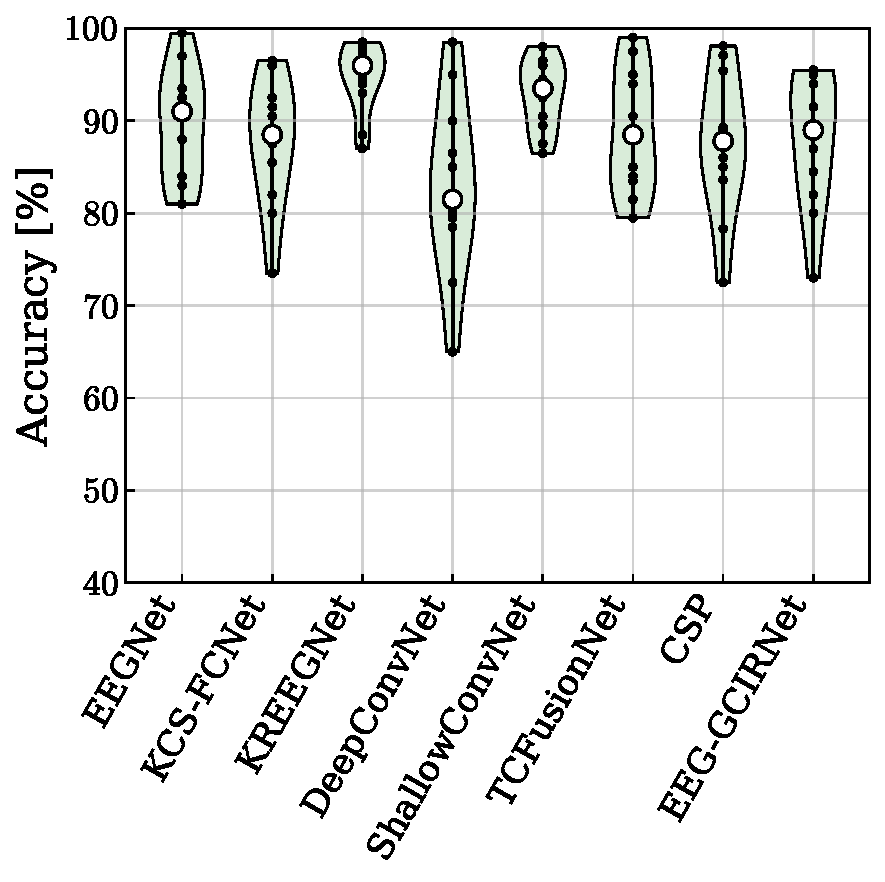
\includegraphics[height=4.5cm]{Figures/violin_good.pdf}}
%          \label{fig:violin_good}
%          \subfloat[]{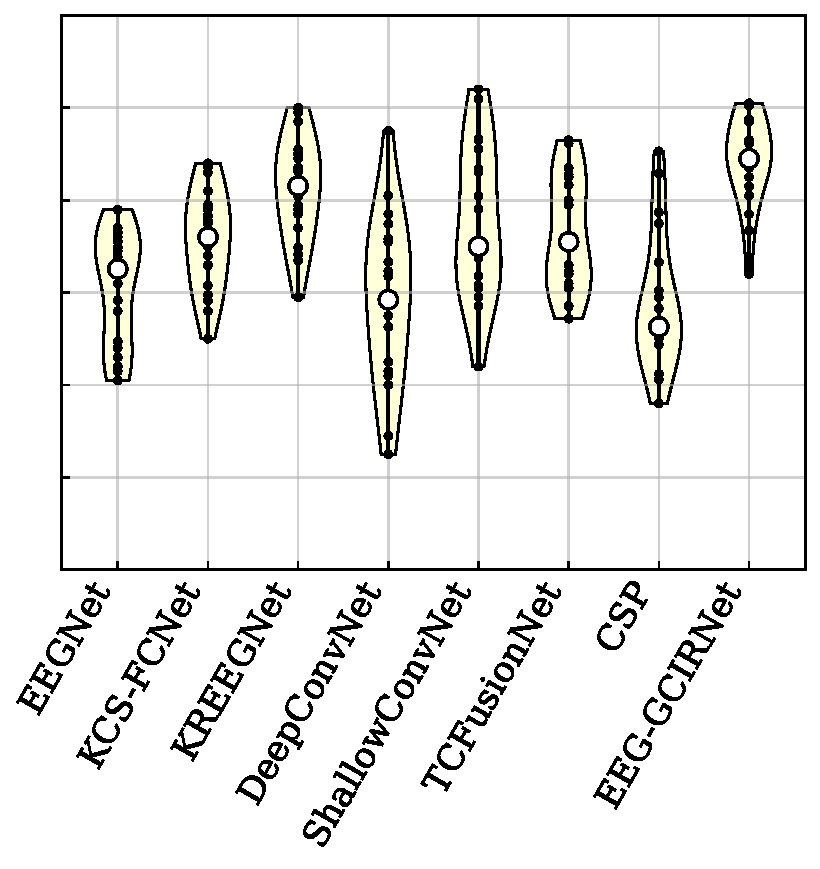
\includegraphics[height=4.5cm]{Figures/violin_mid.pdf}}
%          \label{fig:violin_mid}
%          \subfloat[]{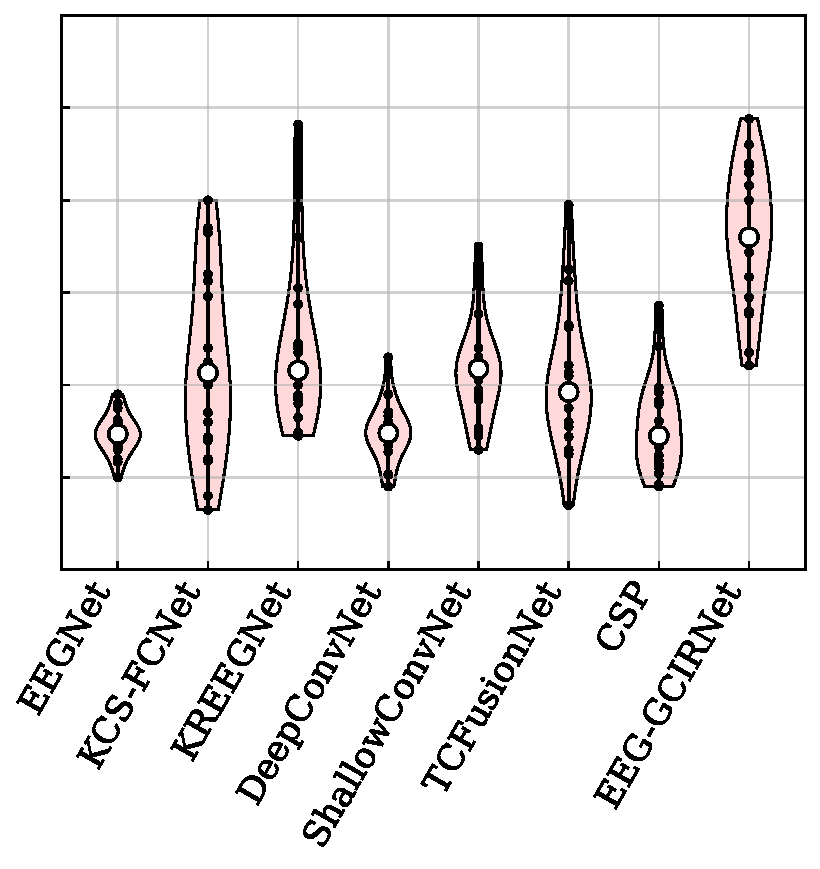
\includegraphics[height=4.5cm]{Figures/violin_bad.pdf}}
%          \label{fig:violin_bad}

%     \caption{Group performing MI-\gls{eeg}classification results. The white dot in each violin plot indicates the median accuracy, while the thick black bar represents the interquartile range. The corresponding average (mean) accuracies for EEGNet and EEG-GCIRNet are reported in Table~\ref{tab:accuracy_gain}.(\textbf{a})
%  Subjects with EEGNet accuracy above 80$\%$. (\textbf{b}) Subjects with EEGNet accuracy between 60$\%$ and 80$\%$. (\textbf{c}) Subjects with EEGNet accuracy below 60$\%$.}
%     \label{fig:Violins}
% \end{figure}
% %-----------------------------------------------
%-----------------------------------------------
\begin{figure}[htbp]
    \centering

    \subfloat[Subjects with EEGNet accuracy above 80\%.]{
        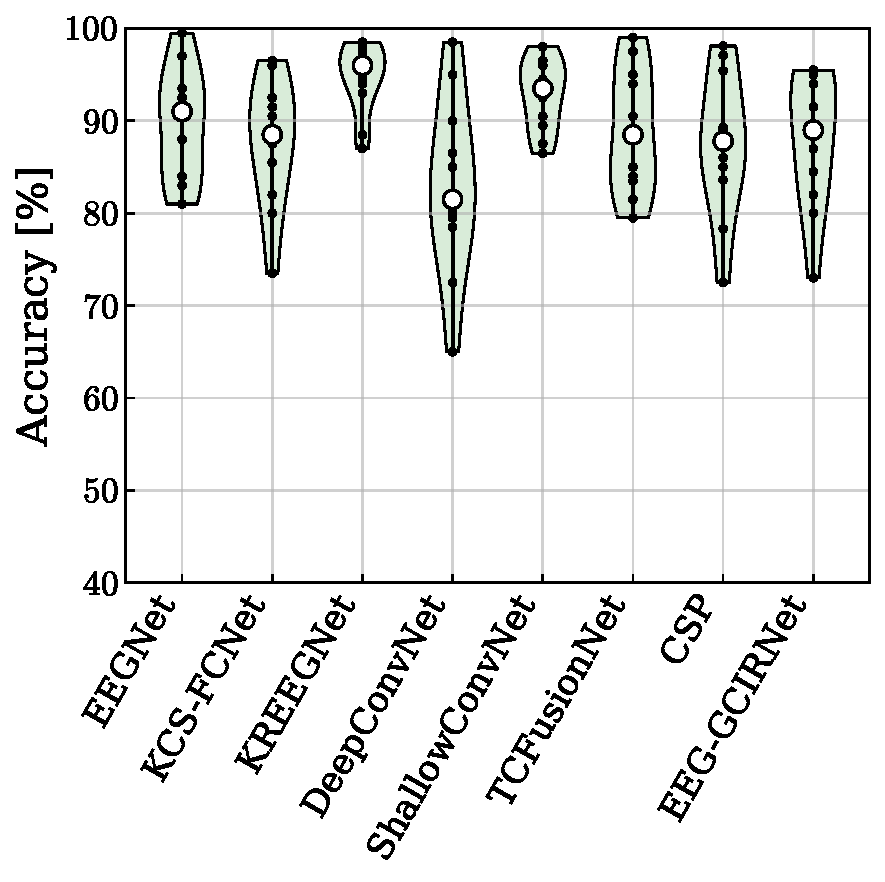
\includegraphics[height=4.8cm]{Figures/violin_good.pdf}
        \label{fig:violin_good}
    }
    \hfill
    \subfloat[Subjects with EEGNet accuracy between 60\% and 80\%.]{
        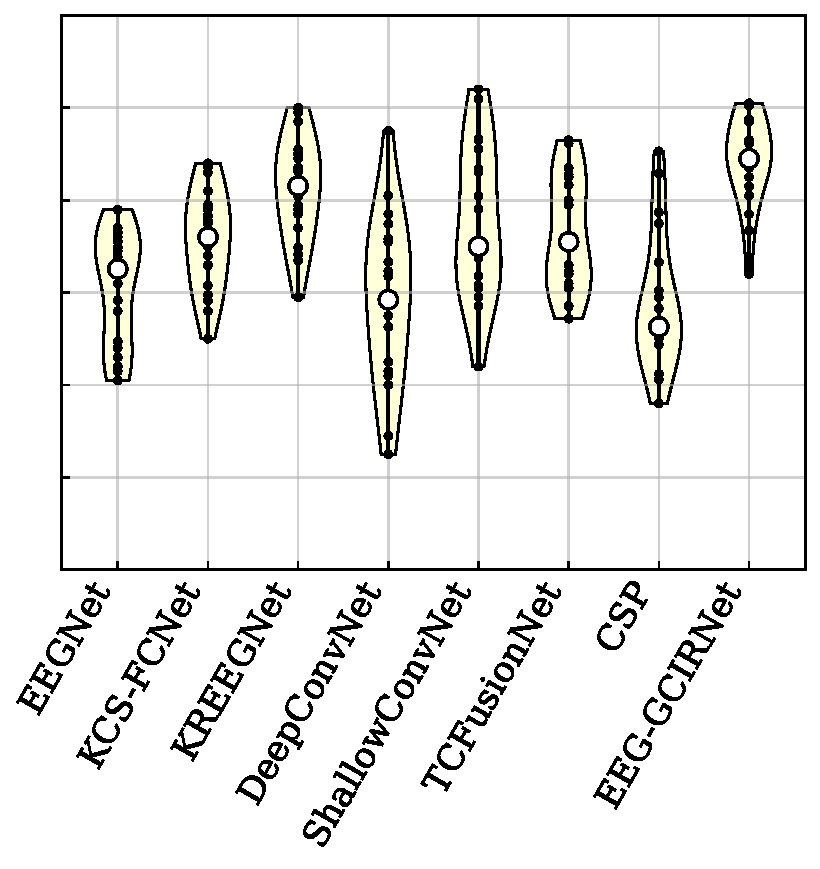
\includegraphics[height=4.8cm]{Figures/violin_mid.pdf}
        \label{fig:violin_mid}
    }
    \hfill
    \subfloat[Subjects with EEGNet accuracy below 60\%.]{
        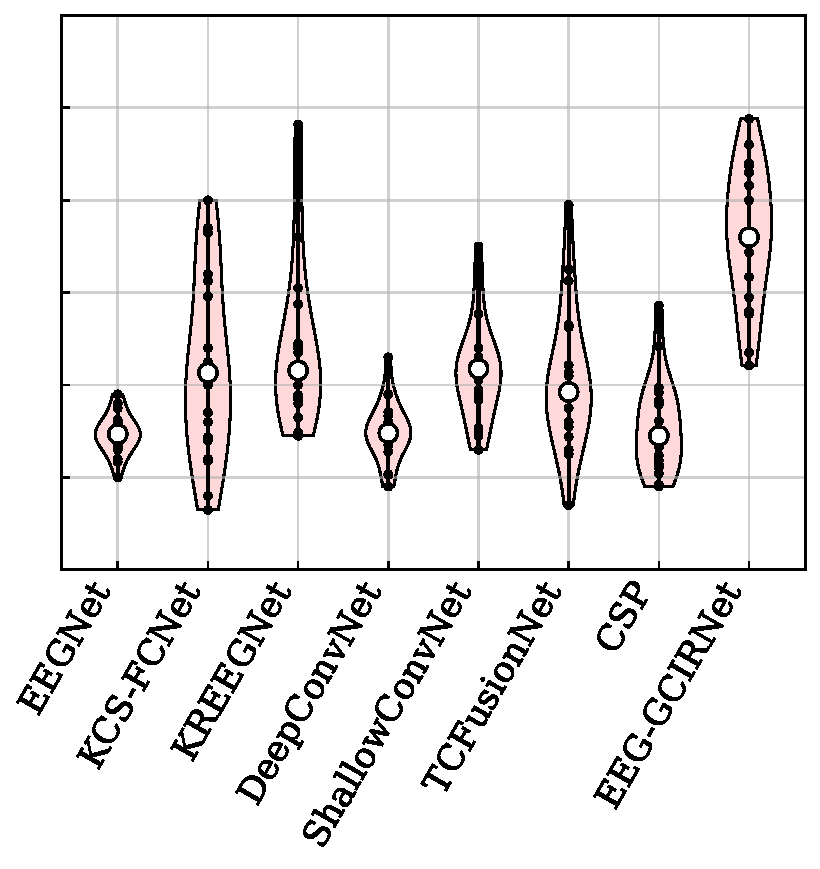
\includegraphics[height=4.8cm]{Figures/violin_bad.pdf}
        \label{fig:violin_bad}
    }

    \caption{Classification performance by subject group for the
    \gls{mi}-\gls{eeg} task. The white dot in each violin plot indicates
    the median accuracy, while the thick black bar represents the
    interquartile range. The corresponding mean accuracies for EEGNet
    and \gls{eeggcirnet} are reported in Table~\ref{tab:accuracy_gain}.}
    \label{fig:Violins}
\end{figure}
%-----------------------------------------------

The most compelling evidence of the model's robustness is found in the ``Bad'' group (Figure~\ref{fig:Violins}c), which reflects the most challenging \gls{eeg} conditions. Here, most models exhibit broad distributions shifted toward low accuracies (40--70\%). Crucially, \gls{eeggcirnet} is the only model for which this group is empty, reaffirming its resilience against signal degradation and its superior stability, as previously suggested by the global accuracy and ranking analyses.


These distributional advantages translate directly into substantial accuracy gains, as summarized in Table~\ref{tab:accuracy_gain}. The improvements are most pronounced for subjects who perform poorly with baseline models. In the ``Bad'' group, where EEGNet achieves an average accuracy of only 54.65\%, \gls{eeggcirnet} provides a remarkable $\sim$22\% increase, elevating the average performance to 76.20\%. A substantial gain of $\sim$14\% is also observed in the ``Mid'' group. Conversely, for the ``Good'' group, where the baseline performance is already high, \gls{eeggcirnet} maintains a comparable accuracy with only a slight decrease ($\sim$2\%). This confirms that the significant gains for challenging cases are not achieved at the expense of performance in high-quality signal conditions.

%------------------------------------------------
\begin{table}[H]%[htbp]
    \caption{Accuracy and gain by {subject performance group} and approach.}
   {
    \begin{tabularx}{\textwidth}{CCCC}
       \toprule
       \textbf{Approach} & \textbf{Group} & \textbf{Accuracy (\%)} & \textbf{Gain (\%)} \\
       \midrule
       \multirow{3}{*}{EEGNet}
         & Good    & 89.64 & --    \\
         & Mid     & 70.54 & --    \\
         & Bad     & 54.65 & --    \\
       \midrule
       \multirow{3}{*}{EEG-GCIRNet (Ours)}
         & Good    & 87.86 & $-1.78$     \\
         & Mid     & 84.24 & $13.70$    \\
         & Bad     & 76.20 & $21.55$    \\
       \bottomrule
    \end{tabularx}}
    \label{tab:accuracy_gain}
\end{table}
%------------------------------------------------
%------------------------------------------------
\begin{figure}[H]
  
\hspace{-12pt}  \resizebox{\linewidth}{!}{% --------- Dimensiones y colores ----------
\def\FigW{20cm}
\def\FigH{8.5cm}

\definecolor{EEGNetDark}{HTML}{7CD8E2}
\definecolor{EEGNetLight}{HTML}{CAEBF1}
\definecolor{CIRNetDark}{HTML}{98D891}
\definecolor{CIRNetLight}{HTML}{ABE3A1}

% --------- Estilos ----------
\pgfplotsset{
  myaxis/.style={
    width=\FigW, height=\FigH,
    ymin=40, ymax=100,
    ylabel={Accuracy [\%]},
    ylabel style={font=\small},
    ytick={40,60,...,100},
    xtick pos=bottom, ytick pos=left,
    tick align=inside,
    ticklabel style={font=\scriptsize},
    axis lines=box,
    tick style={black!60},
    xmajorgrids, ymajorgrids,
    grid style={black!15},
  },
  methodline/.style={
    line width=1.1pt,
    mark=*,
    mark size=1.6pt,
    mark options={solid, draw=#1, fill=#1},
    draw=#1
  },
  bandstyle/.style={draw=none, fill opacity=0.40},
}

% --------- Datos ---------
\pgfplotstableread[row sep=\\, col sep=space]{
subj  eegnet  nrvae  seeg  sgc \\
  43   99.50   94.00   4.64  4.64 \\
  14   97.00   95.50   1.87  1.87 \\
  3    93.50   93.00   4.06  6.00 \\
  50   92.50   84.50   4.58  4.58 \\
  48   92.50   95.00   2.24  2.24 \\
  4    91.00   92.00   6.12  4.80 \\
  35   88.00   82.00   6.96  6.96 \\
  23   84.00   89.00   3.39  3.39 \\
  13   84.00   87.00   2.45  2.45 \\
  41   83.00   80.00   7.75  7.75 \\
  1    81.00   75.00   5.10  5.70 \\
  49   78.97   90.26   2.99  2.99 \\
  37   77.00   85.00   7.31  6.52 \\
  26   76.50   88.50   5.15  3.00 \\
  5    76.50   84.50   7.35  6.20 \\
  44   76.00   90.50   5.61  5.34 \\
  6    75.56   76.67   4.51  4.51 \\
  47   74.87   90.26   5.23  2.51 \\
  28   74.50   86.50   6.96  5.39 \\
  36   73.85   86.15   2.99  4.76 \\
  12   72.57   72.00   7.54  7.54 \\
  39   71.00   78.50   6.04  6.04 \\
  46   69.17   88.75   4.64  1.67 \\
  10   68.00   86.50   9.41  8.15 \\
  20   64.71   83.53   3.72  6.86 \\
  22   64.00   82.50   6.44  6.12 \\
  31   63.00   84.00   9.92  6.44 \\
  18   62.00   84.50   5.34  4.85 \\
  52   61.50   80.50   6.63  8.86 \\
  25   60.50   81.50   11.11 6.25 \\
  21   59.00   84.00   4.64  4.64 \\
  40   58.00   80.00   9.62  9.62 \\
  24   57.50   83.00   4.85  4.85 \\
  27   56.22   62.16   6.71  6.40 \\
  30   56.00   81.60   8.24  8.24 \\
  51   55.90   74.36   3.40  7.78 \\
  42   55.50   86.00   5.83  5.83 \\
  16   55.00   76.00   10.56 10.56 \\
  9    55.00   83.75   3.33  3.33 \\
  38   54.87   67.69   7.71  7.71 \\
  11   54.50   75.50   8.28  8.28 \\
  19   54.48   71.72   9.61  9.61 \\
  33   54.00   76.00   4.64  3.00 \\
  2    54.00   76.00   9.95  10.68 \\
  17   53.50   69.50   3.74  9.41 \\
  15   53.33   80.00   4.10  2.51 \\
  45   53.00   68.00   6.60  5.34 \\
  32   52.00   63.50   8.57  4.64 \\
  7    51.67   88.75   10.32 10.83 \\
  8    50.00   76.50   8.22  5.15 \\
}\datatable

\begin{tikzpicture}
\begin{axis}[
  myaxis,
  enlarge x limits=0,
  enlarge y limits=false,
  trim axis left, trim axis right,
  xlabel={Subjects},
  symbolic x coords={
    43,14,3,50,48,4,35,23,13,41,1,49,37,26,5,44,6,47,28,36,12,39,46,10,
    20,22,31,18,52,25,21,40,24,27,30,51,42,16,9,38,11,19,33,2,17,15,45,32,7,8
  },
  xtick=data,
  x tick label style={rotate=90, anchor=east},
  legend style={
    at={(rel axis cs:0.001,0.001)}, anchor=south west,
    draw=black!40, fill=white, fill opacity=0.9, font=\small,
    rounded corners=2pt
  },
  legend cell align=left,
]

% ===== EEGNet (banda + línea) =====
\addplot[name path=EEGNetUpper, draw=none, forget plot]
  table [x=subj, y expr=\thisrow{eegnet}+\thisrow{seeg}] {\datatable};
\addplot[name path=EEGNetLower, draw=none, forget plot]
  table [x=subj, y expr=\thisrow{eegnet}-\thisrow{seeg}] {\datatable};
\addplot[bandstyle, fill=EEGNetLight, forget plot]
  fill between[of=EEGNetUpper and EEGNetLower];
\addplot[methodline={EEGNetDark}]
  table [x=subj, y=eegnet] {\datatable};

% ===== EEG-CIRNet (banda + línea) =====
\addplot[name path=CIRNetUpper, draw=none, forget plot]
  table [x=subj, y expr=\thisrow{nrvae}+\thisrow{sgc}] {\datatable};
\addplot[name path=CIRNetLower, draw=none, forget plot]
  table [x=subj, y expr=\thisrow{nrvae}-\thisrow{sgc}] {\datatable};
\addplot[bandstyle, fill=CIRNetLight, forget plot]
  fill between[of=CIRNetUpper and CIRNetLower];
\addplot[methodline={CIRNetDark}]
  table [x=subj, y=nrvae] {\datatable};

% ===== Leyenda con el MISMO color de las líneas =====
\addlegendimage{line legend, draw=EEGNetDark, mark=*}
\addlegendentry{EEGNet}
\addlegendimage{line legend, draw=CIRNetDark, mark=*}
\addlegendentry{EEG-GCIRNet}

\end{axis}
\end{tikzpicture}}
  \caption{Inter-subject classification accuracies of EEGNet and \gls{eeggcirnet}. Each point represents the average performance per subject, with subjects ordered according to EEGNet accuracy to highlight the comparative improvements achieved by \gls{eeggcirnet}. Shaded regions indicate \mbox{performance variability}.}
  \label{fig:gains}
\end{figure}
Figure~\ref{fig:gains} illustrates the subject-specific improvements of \gls{eeggcirnet} over the EEGNet baseline, providing direct visual evidence of our framework's corrective capability. Since the performance groups were stratified based on EEGNet's accuracy, the figure demonstrates our model's ability to significantly elevate the performance of users who struggle with conventional BCI systems, thereby directly addressing the challenge of BCI illiteracy. While most participants benefit from moderate accuracy gains, a notable subset—including subjects $21$, $40$, $24$, $30$, $42$, $9$, $15$, and $7$ exhibit a pronounced transition from ``Bad'' to ``Good'' performance levels. For several of these individuals (e.g., subjects $24$, $9$, and $7$), accuracy exceeds the $80\%$ threshold. This performance leap reinforces the hypothesis that latent space modeling in \gls{eeggcirnet} not only mitigates the limitations of signal noise but also provides an effective mechanism for uncovering discriminative structure in signals previously deemed uninformative.

These findings are highly relevant for developing inclusive BCI systems. The fact that several initially low-performing individuals achieve high accuracy suggests that \gls{eeggcirnet} can serve a corrective function within BCI pipelines, enhancing usability and consistency. This benefit extends to ``Mid-performing'' users as well, many of whom are elevated to the high-performing category. This corrective and enhancing capability supports the use of latent generative models in real-world BCI contexts, where adaptability and generalization are critical~\cite{nagarajan2024deeptransfer, gomez2021kernelcca, demir2021autobayes}.

%------------------------------------------------
\subsubsection{Validation on Canonical Scenarios: Binary \gls{mi} Decoding on BCI Competition IV-2a}

The BCI Competition IV-2a dataset constitutes a canonical benchmark for binary \gls{mi} decoding, where the task is restricted to discriminating between left-hand and right-hand \gls{mi} under controlled experimental conditions. In contrast to the multi-class and subject-group validation scenarios analyzed on \gls{eegmmidb} and \gls{adhd}, this dataset enables a direct assessment of the proposed framework’s ability to capture discriminative neural patterns within a highly standardized and widely adopted reference setting in the literature.

The comparative results reported in Table~\ref{tab:acc_comparison} demonstrate that \gls{eeggcirnet} achieves an average accuracy of 88.56\%, placing it among the top-performing methods reported for this binary decoding scenario. This performance clearly surpasses that of widely used convolutional architectures such as EEGNet, DeepConvNet, and ShallowConvNet, which typically achieve accuracies in the 65–68\% range, as well as approaches based on statistical features and classical ensemble strategies, whose performance remains below 65\%.

When compared with more recent methods that incorporate connectivity information or attention-based mechanisms, such as GAT+PLV, \gls{eeggcirnet} exhibits a substantial improvement, with an approximate gain of 16.7 percentage points. This increase suggests that integrating functional connectivity representations structured as topographic maps provides a significant advantage even in binary classification scenarios, where decision boundaries are relatively simpler than those encountered in multi-class \gls{mi} tasks.

%---------------------------------------------------------------------------------
\begin{figure}[htbp]
 \hspace{-12pt}\resizebox{\linewidth}{!}{%

% --------- Dimensiones y colores ----------
\def\FigW{20cm}
\def\FigH{8.5cm}

\definecolor{EEGNetDark}{HTML}{7CD8E2}
\definecolor{EEGNetLight}{HTML}{CAEBF1}
\definecolor{CIRNetDark}{HTML}{98D891}
\definecolor{CIRNetLight}{HTML}{ABE3A1}

% --------- Estilos ----------
\pgfplotsset{
  myaxis/.style={
    width=\FigW, height=\FigH,
    ymin=45, ymax=101,
    ylabel={Accuracy [\%]},
    ylabel style={font=\small},
    ytick={45,50,60,70,80,90,100},
    xtick pos=bottom, ytick pos=left,
    tick align=inside,
    ticklabel style={font=\scriptsize},
    axis lines=box,
    tick style={black!60},
    xmajorgrids, ymajorgrids,
    grid style={black!15},
  },
  methodline/.style={
    line width=1.1pt,
    mark=*,
    mark size=1.6pt,
    mark options={solid, draw=#1, fill=#1},
    draw=#1
  },
  bandstyle/.style={draw=none, fill opacity=0.40},
}

% --------- Datos (ordenados por ACC EEGNet de MAYOR a MENOR) ---------
\pgfplotstableread[row sep=\\, col sep=space]{
subj  eegnet  eegnet_std   cir   cir_std \\
9     74.14   0.00         100.00 0.00 \\
8     70.69   0.00         100.00 0.00 \\
7     70.69   0.00         83.33  0.00 \\
6     65.52   0.00         89.13  0.00 \\
5     63.79   0.00         80.77  0.00 \\
3     63.79   0.00         91.07  0.00 \\
1     63.79   0.00         92.86  0.00 \\
4     55.17   0.00         82.69  0.00 \\
2     46.55   0.00         73.21  0.00 \\
}\datatable

\begin{tikzpicture}
\begin{axis}[
  myaxis,
  enlarge x limits=0,
  xlabel={Subjects},
  symbolic x coords={9,8,7,6,5,3,1,4,2},
  xtick=data,
  x tick label style={rotate=90, anchor=east},
  legend style={
    at={(rel axis cs:0.001,0.001)}, anchor=south west,
    draw=black!40, fill=white, fill opacity=0.9, font=\small,
    rounded corners=2pt
  },
  legend cell align=left,
]

% ===== EEGNet =====
\addplot[name path=EEGNetUpper, draw=none, forget plot]
  table [x=subj, y expr=\thisrow{eegnet}+\thisrow{eegnet_std}] {\datatable};

\addplot[name path=EEGNetLower, draw=none, forget plot]
  table [x=subj, y expr=\thisrow{eegnet}-\thisrow{eegnet_std}] {\datatable};

\addplot[bandstyle, fill=EEGNetLight, forget plot]
  fill between[of=EEGNetUpper and EEGNetLower];

\addplot[methodline={EEGNetDark}]
  table [x=subj, y=eegnet] {\datatable};

% ===== EEG-GCIRNet =====
\addplot[name path=CIRNetUpper, draw=none, forget plot]
  table [x=subj, y expr=\thisrow{cir}+\thisrow{cir_std}] {\datatable};

\addplot[name path=CIRNetLower, draw=none, forget plot]
  table [x=subj, y expr=\thisrow{cir}-\thisrow{cir_std}] {\datatable};

\addplot[bandstyle, fill=CIRNetLight, forget plot]
  fill between[of=CIRNetUpper and CIRNetLower];

\addplot[methodline={CIRNetDark}]
  table [x=subj, y=cir] {\datatable};

% ===== Leyenda =====
\addlegendimage{line legend, draw=EEGNetDark, mark=*}
\addlegendentry{EEGNet}

\addlegendimage{line legend, draw=CIRNetDark, mark=*}
\addlegendentry{EEG-GCIRNet}

\end{axis}
\end{tikzpicture}
}
\caption{{Inter-subject classification accuracies for EEGNet and EEG-GCIRNet on BCI Competition IV-2a. Subjects are ordered according to their EEGNet accuracy.}}
\label{fig:acc_eegnet_vs_eegcirnet_bcic2a}
\end{figure}
%---------------------------------------------------------------------------------

Beyond the aggregate performance comparison summarized in Table~\ref{tab:acc_comparison}, a more fine-grained subject-wise analysis is provided in Fig.~\ref{fig:acc_eegnet_vs_eegcirnet_bcic2a}. This figure contrasts the inter-subject accuracies obtained by EEGNet and the proposed \gls{eeggcirnet} on the BCI Competition IV-2a dataset, with subjects ordered according to EEGNet performance. The visualization reveals that \gls{eeggcirnet} consistently outperforms EEGNet across all subjects, including those exhibiting lower baseline accuracies under the conventional convolutional architecture. Notably, the largest performance gains are observed for subjects with poorer EEGNet performance, indicating an enhanced robustness of the proposed connectivity-driven representation to inter-subject variability. These results suggest that modeling functional connectivity through structured topographic maps allows \gls{eeggcirnet} to capture subject-specific discriminative patterns that are insufficiently exploited by purely channel-wise convolutional approaches, even in canonical binary \gls{mi} decoding scenarios.

It is also noteworthy that the performance of \gls{eeggcirnet} is comparable to that of high-complexity models such as CTNet and CNNViT-MILF-a, which report similarly high accuracies but, in some cases, on different datasets (BCI Competition IV-2b) or using considerably heavier architectures. In this context, the results obtained by \gls{eeggcirnet} reinforce the notion that an informative and physiologically consistent representation can be as decisive as increasing architectural complexity in achieving high performance for \gls{mi} decoding.

%-------------------------------------------------------------------------
\begin{table}[H]
    \centering
    \caption{Average classification accuracy of state-of-the-art methods for binary MI-\gls{eeg} decoding (Left vs. Right) on BCI Competition IV Dataset IIa.}
    \label{tab:acc_comparison}
    \begin{tabularx}{\textwidth}{CC}
        \toprule
        \textbf{Model} & \textbf{ACC [\%]} \\
        \midrule
        DeepConvNet~\cite{schirrmeister2017deep} 
        & $67.62$ \\
        
        ShallowConvNet~\cite{schirrmeister2017deep} 
        & $66.41$ \\
        
        EEGNet~\cite{lawhern2018eegnet} 
        & $65.49$ \\
        
        TE$\kappa_\alpha$~\cite{de2019data} 
        & $68.80$ \\
        
        StatFeat-Ensemble v1~\cite{Degirmenci2023} 
        & $61.86$ \\
        
        StatFeat-Ensemble v2~\cite{Degirmenci2024} 
        & $63.04$ \\
        
        GAT+PLV~\cite{patel2025advancing} 
        & $71.89$ \\
        
        CTNet$^{\dagger}$~\cite{CTNet} 
        & $88.49$ \\
        
        CNNViT\text{-}MILF\text{-}a$^{\dagger}$~\cite{CNNViT} 
        & $81.11$ \\
        
        \textbf{EEG-GCIRNet (Ours)} 
        & $\mathbf{88.56}$ \\
        \bottomrule
    \end{tabularx}

    \vspace{4pt}
    \footnotesize{\textbf{Note.} $^{\dagger}$ Accuracy reported on BCI Competition IV-2b for two-class left/right motor imagery classification.}
\end{table}
%-------------------------------------------------------------------------

\subsubsection{Validation on Complex Scenarios: Multi-Class Decoding on \gls{eegmmidb} Collection}

{To assess the scalability of the proposed framework beyond binary classification, we evaluated its performance on the \gls{eegmmidb} dataset, which involves a challenging $5$-class \gls{mi} task. This scenario requires the model to disentangle multiple distinct neural patterns (Left Hand, Right Hand, Both Hands, Both Feet, and Rest), significantly increasing the complexity of the decision boundaries compared to the GigaScience benchmark.}

{Table~\ref{tab:acc_5class_results} presents the comparative results against a curated set of state-of-the-art architectures. These baselines were selected to represent the broad spectrum of current deep learning strategies for \gls{eeg}decoding: {EEGNet} serves as the compact, general-purpose benchmark; {DeepConvNet} and {ShallowConvNet} represent established end-to-end architectures that optimize temporal and spatial filters directly from raw data; and {TCFusionNet} is included to represent recent advancements in complex temporal-channel fusion mechanisms. Against this diverse backdrop of raw signal decoders, \gls{eeggcirnet} achieves the highest average accuracy of $75.20 \pm 4.63\%$, surpassing all baseline models by a considerable margin. While reference architectures such as TCFusionNet and DeepConvNet plateau around $\sim 68\%$ (with $68.89\%$ and $68.35\%$ respectively), our approach yields a net performance gain of approximately $6.3\%$. This superiority is particularly notable given the difficulty of the task, suggesting that the connectivity-driven topographic maps provide a richer feature space than raw temporal signals for distinguishing between spatially overlapping classes, such as ``Both Hands'' versus single-hand imagery.}

\begin{table}[H]%[ht!]
    
    \caption{{MI-\gls{eeg}5-class classification performance comparison: 
    Average ACC $\pm$ standard deviation across the $10$ considered subjects.}}
    {
    \begin{tabularx}{\textwidth}{CC}
        \toprule
        \textbf{Model} & \textbf{ACC [\%]} \\
        \midrule
        % CSP~\cite{ang2008filter} &  \\
        EEGNet~\cite{lawhern2018eegnet} & $67.94 \pm 3.98$ \\
        % KREEGNet~\cite{computers12070145} &  \\
        % KCS-FCNet~\cite{diagnostics13061122} &  \\
        DeepConvNet~\cite{schirrmeister2017deep} & $68.35 \pm 4.11$ \\
        ShallowConvNet~\cite{Kim2022} & $67.90 \pm 4.06$ \\
        TCFusionNet~\cite{Musallam2021} & $68.89 \pm 3.90$ \\
        \textbf{EEG-GCIRNet (Ours)} & $\mathbf{75.20 \pm 4.63}$ \\
        \bottomrule
    \end{tabularx}}
    \label{tab:acc_5class_results}
\end{table}

The robustness of these findings is visually confirmed in Figure~\ref{fig:acc_5}, which details subject-wise accuracy sorted by baseline performance. \gls{eeggcirnet} maintains a strict performance advantage across the entire cohort, with the green curve remaining consistently above the baseline. This superiority is particularly pronounced for the most challenging subjects (e.g., Subjects 8, 49, and 7); while the baseline model's performance degrades towards $65\%$, the proposed framework exhibits a corrective behavior, stabilizing accuracies above $71\%$ achieving the highest accuracy with $\sim$78\% for subject 7. Furthermore, the narrower confidence intervals (shaded regions) observed for \gls{eeggcirnet} indicate that the variational regularization effectively mitigates the variability inherent in complex 5-class decision boundaries, yielding not only higher accuracy but greater predictive stability than standard temporal decoding.

Overall, these results confirm that the proposed unimodal VAE framework is not limited to simple binary discrimination but effectively scales to multi-class scenarios, leveraging the latent disentanglement of connectivity patterns to resolve complex \gls{mi} tasks.

\begin{figure}[H]
  
 \hspace{-12pt} \resizebox{\linewidth}{!}{% --------- Dimensiones y colores ----------
\def\FigW{20cm}
\def\FigH{8.5cm}

\definecolor{EEGNetDark}{HTML}{7CD8E2}
\definecolor{EEGNetLight}{HTML}{CAEBF1}
\definecolor{CIRNetDark}{HTML}{98D891}
\definecolor{CIRNetLight}{HTML}{ABE3A1}

% --------- Estilos (MISMO DEL ORIGINAL) ----------
\pgfplotsset{
  myaxis/.style={
    width=\FigW, height=\FigH,
    ymin=60, ymax=80,
    ylabel={Accuracy [\%]},
    ylabel style={font=\small},
    ytick={60,65,70,75,80, 85},
    xtick pos=bottom, ytick pos=left,
    tick align=inside,
    ticklabel style={font=\scriptsize},
    axis lines=box,
    tick style={black!60},
    xmajorgrids, ymajorgrids,
    grid style={black!15},
  },
  methodline/.style={
    line width=1.1pt,
    mark=*,
    mark size=1.6pt,
    mark options={solid, draw=#1, fill=#1},
    draw=#1
  },
  bandstyle/.style={draw=none, fill opacity=0.40},
}

% --------- Datos ordenados por ACC EEGNet ---------
\pgfplotstableread[row sep=\\, col sep=space]{
subj  eegnet  eegnet_std   cir   cir_std \\
13  70.1587  3.0778   77.79  3.7022 \\
50  70.1587  2.7309   77.80  4.0902 \\
12  69.5238  3.9396   77.77  6.8824 \\
9   69.2063  3.8359   76.19  5.0195 \\
40  68.2539  3.3295   76.18  7.0702 \\
7   67.3016  3.8359   77.78  5.4618 \\
41  66.3492  5.2549   71.44  3.5634 \\
49  66.3492  5.2549   73.01 3.4191 \\
3   66.0317  5.0793   71.43  2.5790 \\
8   66.0317  4.7724   73.02  4.4895 \\
}\datatable


\begin{tikzpicture}
\begin{axis}[
  myaxis,
  enlarge x limits=0,
  xlabel={Subjects},
  symbolic x coords={13,50,12,9,40,7,41,49,3,8},
  xtick=data,
  x tick label style={rotate=90, anchor=east},
  legend style={
    at={(rel axis cs:0.001,0.001)}, anchor=south west,
    draw=black!40, fill=white, fill opacity=0.9, font=\small,
    rounded corners=2pt
  },
  legend cell align=left,
]

% ===== EEGNet =====
\addplot[name path=EEGNetUpper, draw=none, forget plot]
  table [x=subj, y expr=\thisrow{eegnet}+\thisrow{eegnet_std}] {\datatable};

\addplot[name path=EEGNetLower, draw=none, forget plot]
  table [x=subj, y expr=\thisrow{eegnet}-\thisrow{eegnet_std}] {\datatable};

\addplot[bandstyle, fill=EEGNetLight, forget plot]
  fill between[of=EEGNetUpper and EEGNetLower];

\addplot[methodline={EEGNetDark}]
  table [x=subj, y=eegnet] {\datatable};

% ===== EEG-GCIRNet =====
\addplot[name path=CIRNetUpper, draw=none, forget plot]
  table [x=subj, y expr=\thisrow{cir}+\thisrow{cir_std}] {\datatable};

\addplot[name path=CIRNetLower, draw=none, forget plot]
  table [x=subj, y expr=\thisrow{cir}-\thisrow{cir_std}] {\datatable};

\addplot[bandstyle, fill=CIRNetLight, forget plot]
  fill between[of=CIRNetUpper and CIRNetLower];

\addplot[methodline={CIRNetDark}]
  table [x=subj, y=cir] {\datatable};

% ===== Leyenda EXACTAMENTE como el código original =====
\addlegendimage{line legend, draw=EEGNetDark, mark=*}
\addlegendentry{EEGNet}

\addlegendimage{line legend, draw=CIRNetDark, mark=*}
\addlegendentry{EEG-GCIRNet}

\end{axis}
\end{tikzpicture}
}
  \caption{{Inter-subject classification accuracies for EEGNet and \gls{eeggcirnet} in the 5-class MI-\gls{eeg}setting. Subjects are ordered according to their EEGNet accuracy to emphasize the consistent performance gains achieved by \gls{eeggcirnet}. Shaded regions denote the accuracy variability \mbox{across trials.}}}
  \label{fig:acc_5}
\end{figure}

{For the multi-class setting, we analyzed the stability of the models through average rankings and assessed the significance of the performance differences using pairwise Wilcoxon signed-rank tests. The summary of these statistical metrics is presented in Table~\ref{tab:p-values_updated1}. \gls{eeggcirnet} achieves a perfect average ranking of ${1.00}$, indicating that it consistently outperformed all reference architectures across the considered subjects. This places it significantly ahead of the nearest competitor, TCFusionNet, which obtained an average ranking of $2.15$, and well beyond the standard end-to-end baselines like DeepConvNet ($3.10$) and EEGNet ($4.30$). The statistical reliability of these gains is confirmed by the hypothesis testing analysis. The proposed model yields the lowest average $p$-value (${0.002}$), which is markedly below the standard significance threshold ($\alpha = 0.05$). While TCFusionNet and DeepConvNet also exhibit statistical significance ($p=0.021$ and $p=0.026$, respectively), the order-of-magnitude difference in favor of \gls{eeggcirnet} underscores its robustness. Conversely, shallow and compact architectures such as ShallowConvNet and EEGNet show high $p$-values ($0.25$), suggesting that their performance fluctuations in this complex 5-class scenario lack statistical consistency compared to the proposed approach.}
%-----------------------------------------------
\begin{table}[H]%[ht!]
    \centering
    \caption{Average rankings and average pairwise Wilcoxon $p$-values.}
    \begin{tabularx}{\textwidth}{CCC}
       \toprule
        \textbf{Model} & \textbf{Avg. Ranking} & \textbf{Avg. Wilcoxon \emph{p}-Value} \\
        \midrule
        EEGNet        & $4.30$ & $0.25$ \\
        DeepConvNet   & $3.10$ & $0.026$ \\
        ShallowConvNet& $4.45$ & $0.25$ \\
        TCFusion      & $2.15$ & $0.021$ \\
        \textbf{EEG-GCIRNet (Ours)} & $\mathbf{1.00}$ & $\mathbf{0.002}$ \\
        \bottomrule
    \end{tabularx}
    \label{tab:p-values_updated1}
\end{table}
%-----------------------------------------------

\subsubsection{Subject-Group Validation on the \gls{adhd}/Control Children Dataset Following the SGKF-CV Protocol}

To further assess the generalization capability of the proposed framework under clinically realistic conditions, its performance was evaluated on the \gls{adhd}/control children dataset using a Subject-Group K-Fold Cross-Validation (SGKF-CV) protocol. Unlike conventional random or subject-dependent splits, the SGKF scheme enforces a strict separation of subjects between training and testing folds, thereby preventing any subject overlap. This validation setting poses a substantially more challenging scenario, as it explicitly evaluates the ability of the model to generalize across heterogeneous individuals rather than exploiting subject-specific \gls{eeg}patterns.

Table~\ref{tab:sgkf_accuracy_comparison} reports the accuracy-based performance comparison against a representative set of baseline models spanning classical machine learning methods and modern deep learning architectures for \gls{eeg}decoding. Under this stringent subject-independent evaluation, \gls{eeggcirnet} achieves an average accuracy of $63.50 \pm 3.44\%$. While this result is lower than those obtained by architectures such as T-GARNet, ShallowConvNet, and CNN-LSTM, it provides important insight into the behavior of connectivity-driven representations when confronted with pronounced inter-subject variability, which is characteristic of pediatric \gls{adhd} cohorts.

It is important to note that, in the \gls{adhd}/control children dataset, the dominant source of difficulty shifts from class separability—as observed in the multi-class \gls{eegmmidb} experiments—toward robust subject-to-subject transfer. In this context, performance improvements depend not only on the expressive power of the learned features but also on their invariance across subjects, recording sessions, and neurophysiological profiles. The observed performance gap relative to top-performing baselines suggests that additional mechanisms aimed at reducing domain shift, such as explicit domain alignment or adaptive normalization strategies, may be required to fully exploit connectivity-based representations in this setting. Nevertheless, the relatively moderate standard deviation across folds indicates that \gls{eeggcirnet} maintains stable behavior under SGKF-CV, highlighting its training robustness despite the challenging validation protocol.

Overall, these results confirm that the \gls{adhd}/control children dataset constitutes a substantially more demanding generalization scenario compared to subject-dependent or multi-class decoding tasks. While the proposed connectivity-driven framework demonstrates consistent and stable performance under strict subject-group validation, the comparison in Table~\ref{tab:sgkf_accuracy_comparison} also delineates clear opportunities for enhancing inter-subject robustness in clinical \gls{eeg}decoding applications, which remains a central challenge for practical BCI deployment.

%-------------------------------------------------------------------------
\begin{table}[H]
    \centering
    \caption{Performance comparison under the SGKF-CV protocol using accuracy as the evaluation metric. Accuracy is reported as mean $\pm$ standard deviation.}
    \label{tab:sgkf_accuracy_comparison}
    \begin{tabularx}{\textwidth}{CC}
        \toprule
        \textbf{Model} & \textbf{ACC [\%]} \\
        \midrule
        T-GARNet~\cite{salazar2025tgarnet} 
        & $\mathbf{82.07 \pm 3.07}$ \\
        
        ShallowConvNet~\cite{schirrmeister2017deep} 
        & $81.91 \pm 1.36$ \\
        
        CNN-LSTM~\cite{wang2022cnnlstm_adhd} 
        & $80.21 \pm 3.96$ \\
        
        EEGNet~\cite{lawhern2018eegnet} 
        & $75.61 \pm 4.60$ \\
        
        Multi-Stream Transformer~\cite{delvigne2022icpr_transformer_attention} 
        & $73.39 \pm 5.94$ \\
        
        ANOVA-PCA SVM~\cite{alim2023signals_anovapca_svm} 
        & $66.47 \pm 0.00$ \\
        
        IM-CBGT~\cite{alsharif2024aims_imcbgt} 
        & $64.98 \pm 0.78$ \\
        
        \textbf{EEG-GCIRNet ({Ours})} 
        & $63.50 \pm 3.44$ \\
        \bottomrule
    \end{tabularx}
\end{table}
%-------------------------------------------------------------------------

% \subsubsection{Interpretability and Internal Model Dynamics}

% To understand the mechanisms behind EEG-GCIRNet's robust performance, we analyzed its internal dynamics and learned representations. The results reveal that the model is not a ``black box'' but a structured framework that adapts its learning strategy, captures physiologically meaningful patterns, and creates an effective feature space.

To understand the mechanisms behind \gls{eeggcirnet}'s robust performance, we analyzed its internal dynamics and learned representations. The results reveal that the model is not a ``black box'', but rather a structured framework that adapts its learning strategy, captures physiologically meaningful patterns, and creates an effective feature space. {This interpretability analysis is organized around three complementary perspectives: the reorganization of the loss-function weights, the behavior of the latent space, and the temporal, spatial, and spectral patterns learned by the model. Together, these analyses provide insight into how \gls{eeggcirnet} balances reconstruction, classification, and regularization while preserving discriminative EEG information across different subject-performance groups.}

{This subsection provides an integrated analysis of how \gls{eeggcirnet} organizes its internal representations during training and how these representations support robust MI decoding. Rather than evaluating interpretability only through post-hoc visual explanations, the analysis considers complementary aspects of the model behavior, including the reorganization of loss-function weights, the balance between reconstruction and classification objectives, the structure of the latent space, and the temporal, spatial, and spectral patterns learned by the network. Together, these elements allow the model dynamics to be interpreted not only in terms of predictive performance, but also in terms of how discriminative and physiologically meaningful EEG information is preserved across different subject-performance groups.}

{In this sense, the interpretability analysis aims to show whether the proposed framework learns stable connectivity-driven representations, whether these representations remain consistent under different levels of subject variability, and whether the model relies on EEG patterns that are compatible with known MI-related neurophysiological mechanisms. The following subsections therefore examine the internal behavior of \gls{eeggcirnet} from multiple complementary perspectives.}

\subsubsection{Adaptive Learning Through Loss Weight Reorganization}
%------------------------------------------------
\begin{figure}[H]
    
    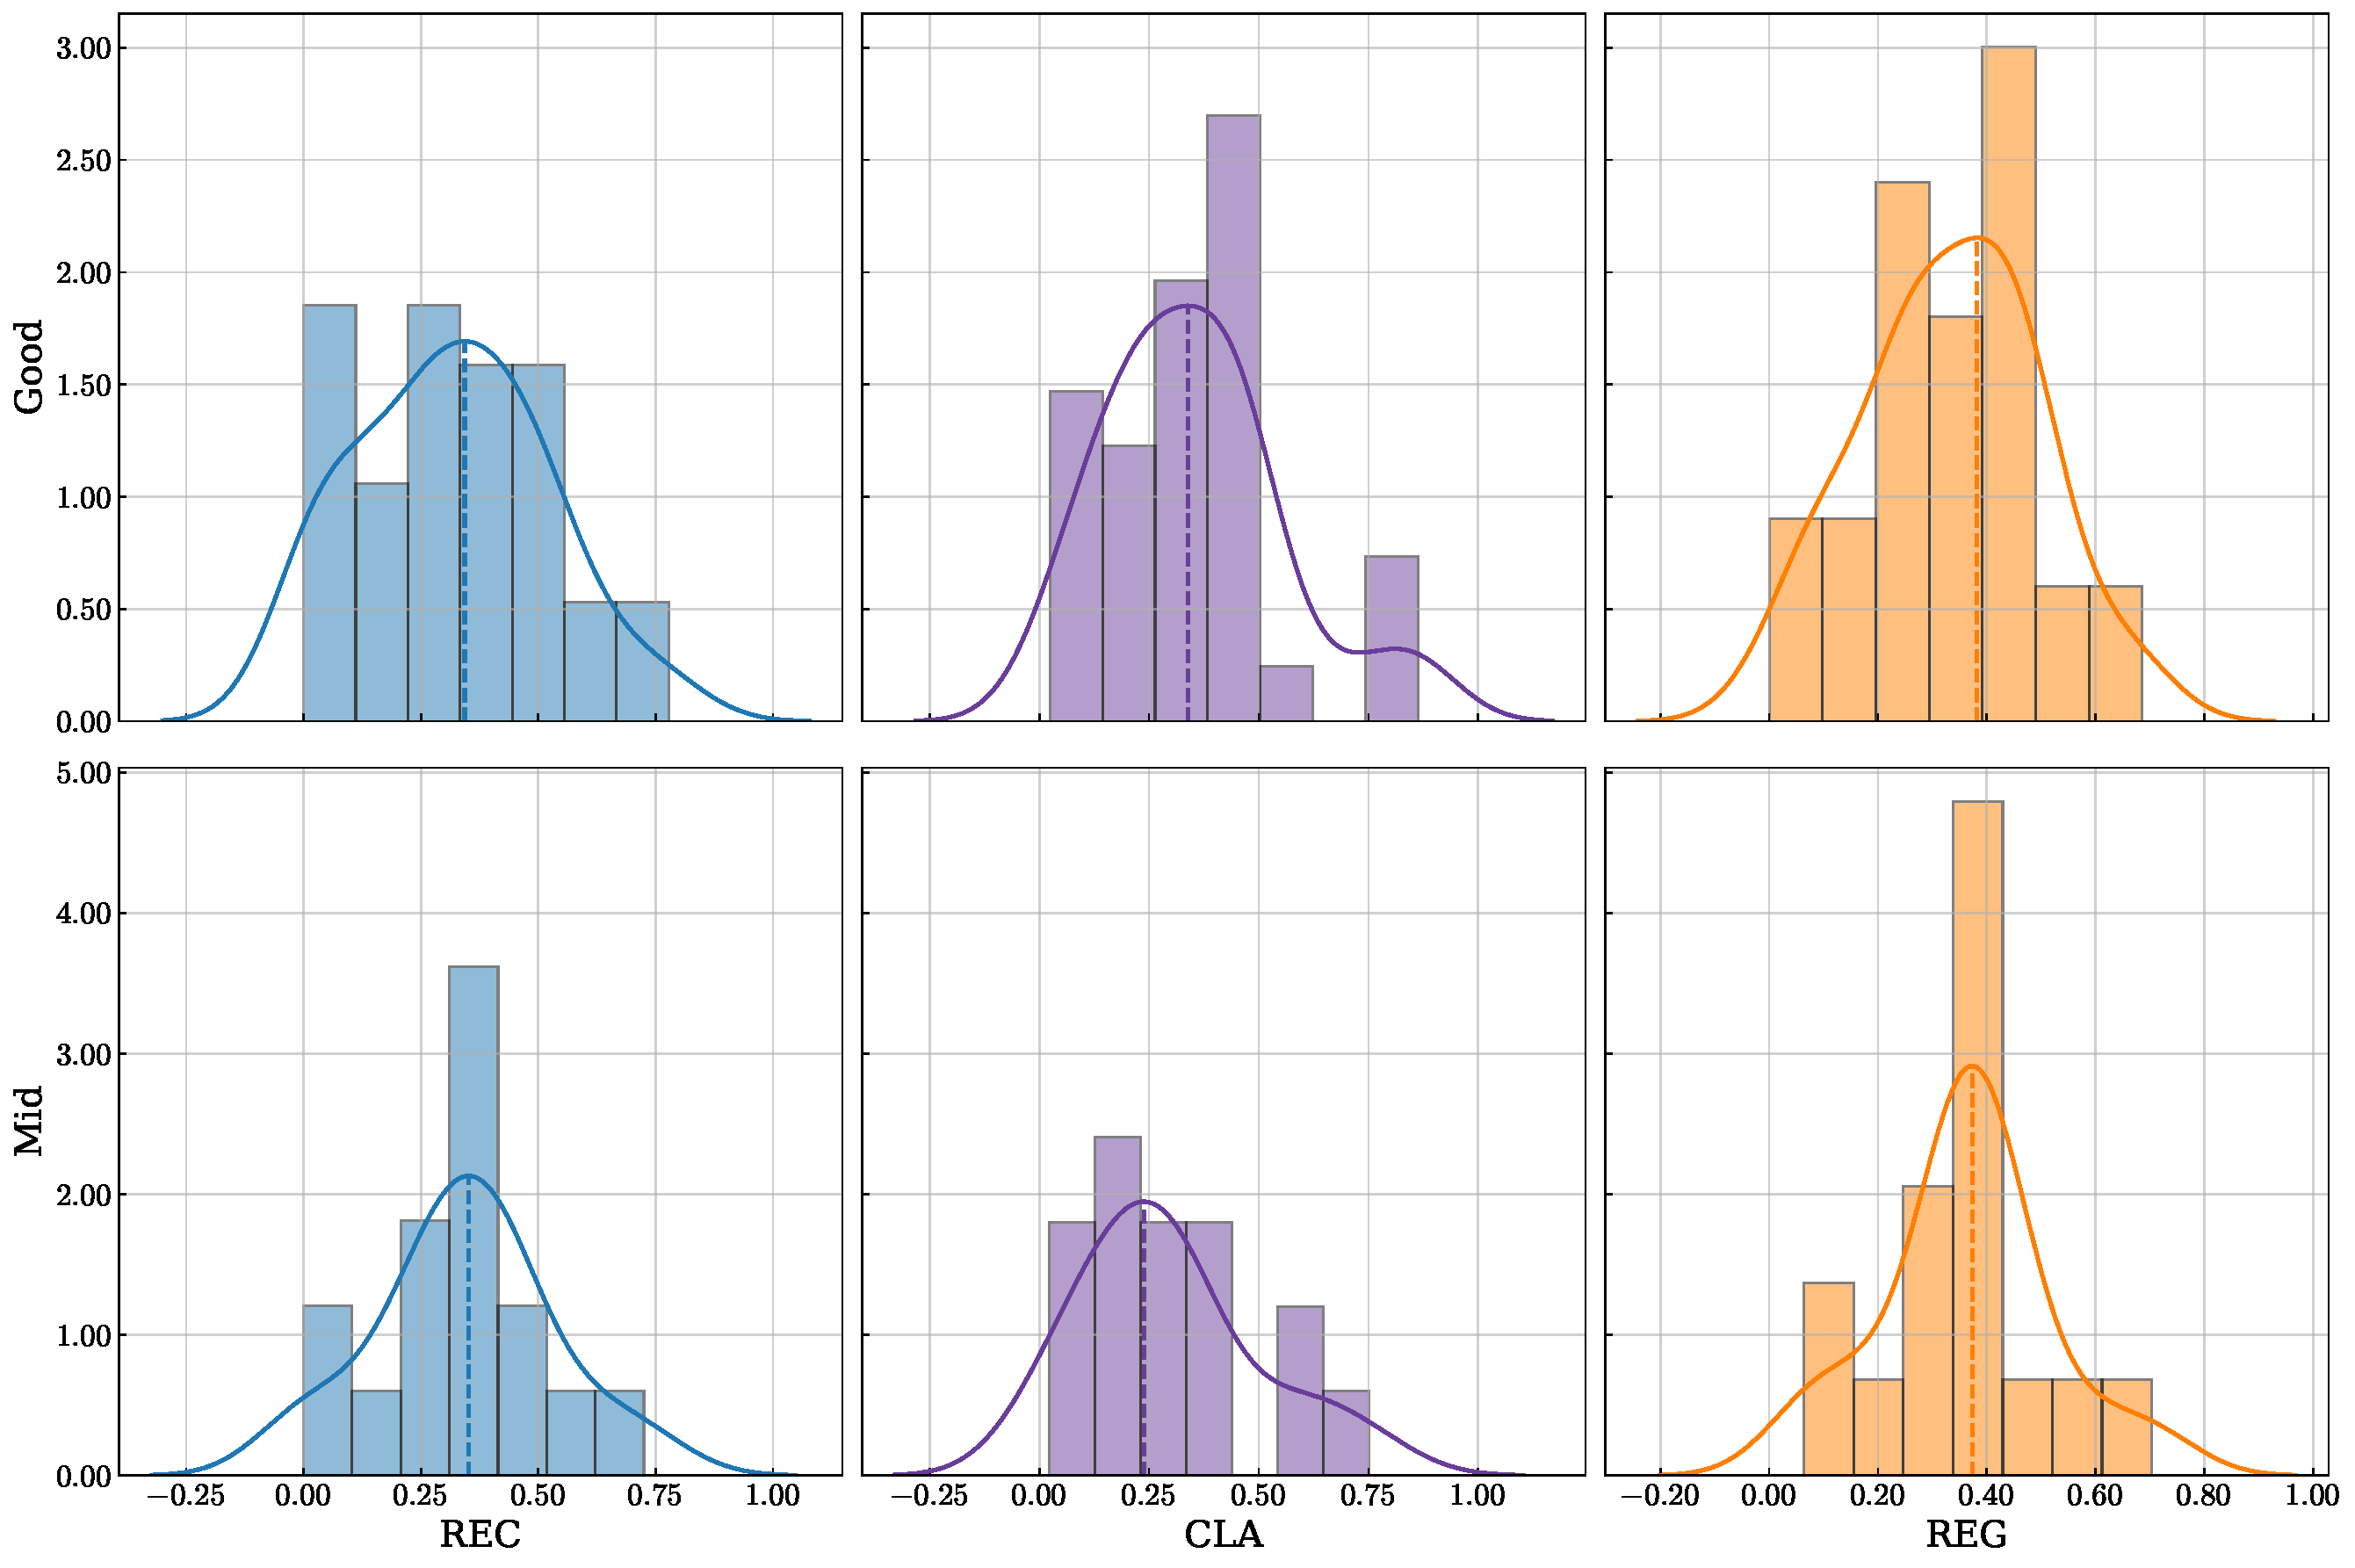
\includegraphics[width=\linewidth]{Figures/distributions_histogram_mid_good_with_mode.pdf}
    \caption{Distributions
 of the weights corresponding to the three loss components—reconstruction (REC), classification (CLA), and latent space regularization (REG)—for the performance groups ``Good'' and ``Mid''. Solid curves represent the density estimates, while dashed vertical lines indicate the mode of each distribution.}
    \label{fig:distributions}
\end{figure}
%------------------------------------------------
A key feature of \gls{eeggcirnet} is its ability to adapt its optimization priorities based on signal quality. The distributions of the three loss component weights, presented in Figure~\ref{fig:distributions}, reveal a distinct internal reorganization between the ``Good'' and ``Mid'' performance groups for the bi-class scenario. This behavior highlights the model’s inherent ability to promote a balanced interaction between reconstruction accuracy, discriminative capacity, and latent space stability. For the ``Good'' group, the weights for reconstruction (REC), classification (CLA), and latent space regularization (REG) are relatively balanced (modes: $0.3433$, $0.3390$, and $0.3824$, respectively). The slight predominance of the REG component suggests a focus on maintaining a coherent latent structure, which aligns with recent findings on the importance of regularization for robust performance~\cite{10483787}. 

In contrast, for the ``Mid'' group, the model distinctly reorganizes its priorities. The REG component remains dominant (mode: $0.3732$), but the CLA weight is significantly reduced (mode: $0.2382$) in favor of REC (mode: $0.3519$). This numerical shift, visible as a change in the central tendency of the distributions in Figure~\ref{fig:distributions}, indicates that when faced with less discriminative signals, the model prioritizes learning a stable and faithful representation of the input data over immediate classification accuracy. This adaptive strategy, where internal representation optimization substitutes for explicit discriminative signals, is a known characteristic of robust unimodal systems~\cite{Dhanushkodi}.
%---------------------------------------------------
%%% graficas hps Giga
%----------------------------------------------------
{To further examine the loss-weight reorganization, pairwise contour maps were built from the hyperparameter search of two representative subjects: Subject~14 from the ``Good'' group and Subject~27 from the ``Mid'' group. By visualizing the explored combinations of reconstruction (REC), classification (CLA), and regularization (REG) weights, these maps reveal how different optimization priorities shape the validation-accuracy landscape in \gls{eeggcirnet}.}

\begin{figure}[H]
\centering

\makebox[\textwidth][c]{%
\begin{minipage}[c]{0.99\textwidth}
\centering

\subfloat[REC vs. CLA]{%
    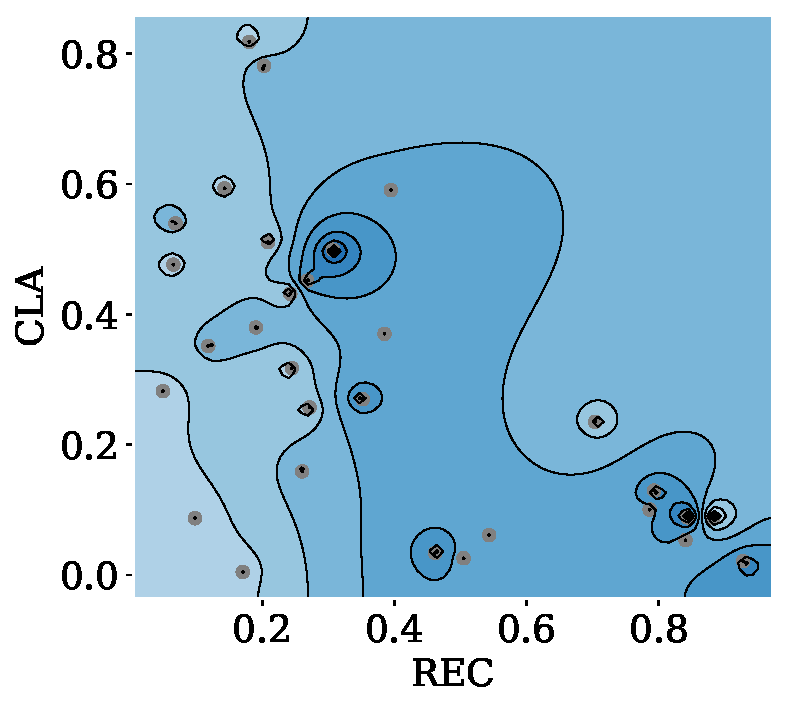
\includegraphics[width=0.34\linewidth,height=3.4cm]{Figures/contour_REC_vs_CLA-14.pdf}
}
\subfloat[REC vs. REG]{%
    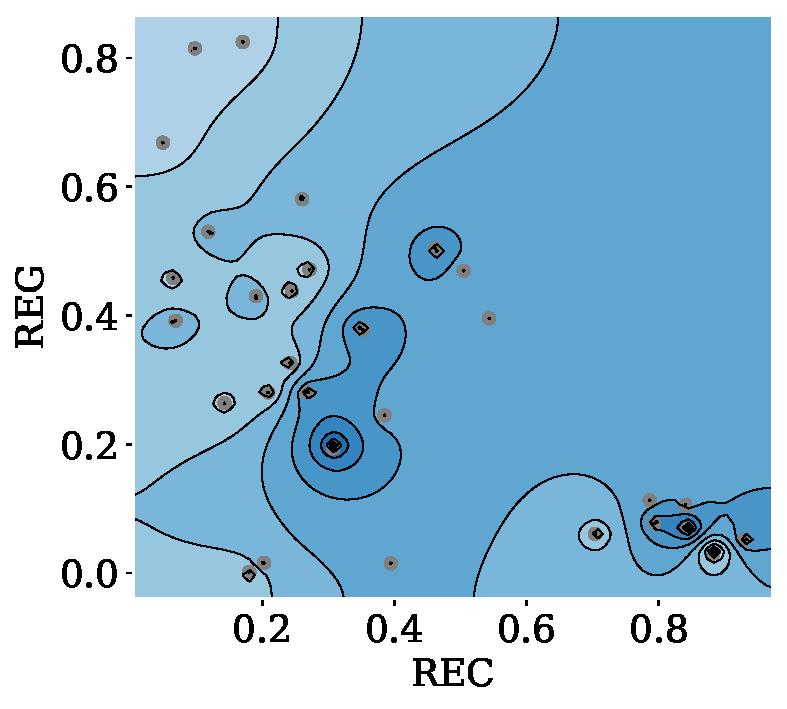
\includegraphics[width=0.34\linewidth,height=3.4cm]{Figures/contour_REC_vs_REG-14.pdf}
}
\subfloat[CLA vs. REG]{%
    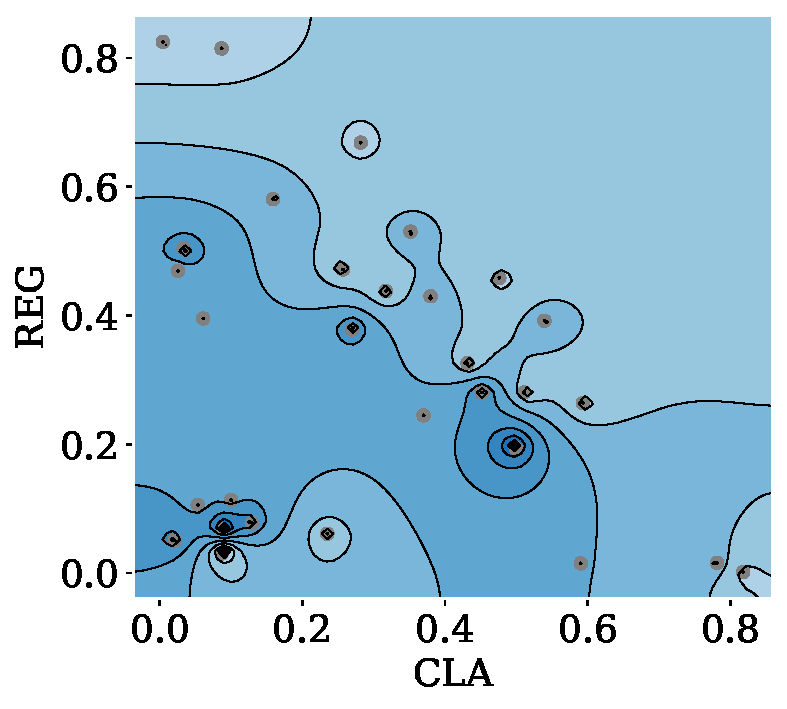
\includegraphics[width=0.34\linewidth,height=3.4cm]{Figures/contour_CLA_vs_REG-14.pdf}
}

\vspace{0.6em}

\begin{tikzpicture}
\begin{axis}[
    hide axis,
    scale only axis,
    width=\linewidth,
    height=0pt,
    colormap name=optunablues,
    colorbar horizontal,
    point meta min=88.4,
    point meta max=94,
    colorbar style={
        width=\linewidth,
        height=3mm,
        xtick={88.4, 89.2, 90, 90.8, 91.6, 92.4, 93.2, 94},
        xticklabel style={font=\scriptsize},
        xlabel={Val. accuracy (\%)},
        xlabel style={font=\scriptsize, yshift=2pt},
        scaled ticks=false,
        /pgf/number format/fixed,
        /pgf/number format/precision=1,
    },
]
\addplot [draw=none] coordinates {(0,0)};
\end{axis}
\end{tikzpicture}

\end{minipage}%
}

\caption{{Contour plots of validation accuracy (\%) as a function of the normalized loss weights REC, CLA, and REG for Subject~14, a representative subject from the ``Good'' group on the GigaScience dataset. All panels share the same color scale, allowing direct visual comparison across loss-weight pairs for this subject.}}
\label{fig:global_freq_GIGA14}
\end{figure}
%----------------------------------------------------
{For Subject~14 (Figure~\ref{fig:global_freq_GIGA14}), which is representative of the ``Good'' performance group, the contour maps reveal a broad and stable high-accuracy region across the explored loss-weight space. In all three pairwise projections, validation accuracy remains within a narrow high-performance range, indicating that the model is not strongly dependent on a single, highly specific combination of REC, CLA, and REG. This suggests that, for subjects with more discriminative EEG patterns, \gls{eeggcirnet} can preserve robust decoding performance under different optimization balances. The presence of extended high-accuracy regions rather than isolated optima indicates that reconstruction, classification, and latent-space regularization interact in a complementary manner, supporting representation stability and reducing abrupt performance degradation~\cite{10483787,Dhanushkodi}. This behavior is consistent with the balanced loss-weight distribution observed for the ``Good'' group in Figure~\ref{fig:distributions}, where the three components contribute relatively evenly to the optimization process.}

%----------------------------------------------------

\begin{figure}[H]
\centering

\makebox[\textwidth][c]{%
\begin{minipage}[c]{0.99\textwidth}
\centering

\subfloat[REC vs. CLA]{%
    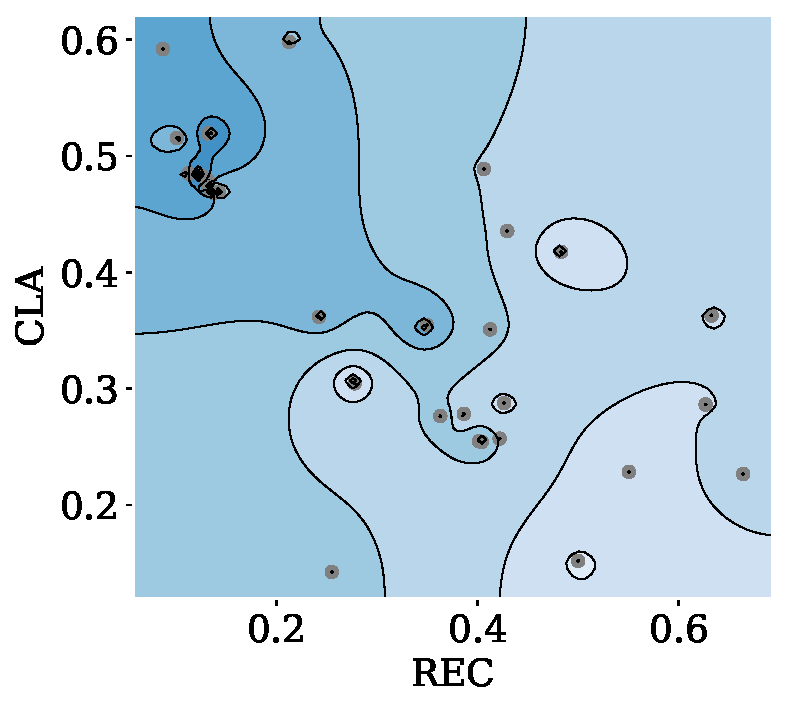
\includegraphics[width=0.34\linewidth,height=3.4cm]{Figures/contour_REC_vs_CLA-27.pdf}
}
\subfloat[REC vs. REG]{%
    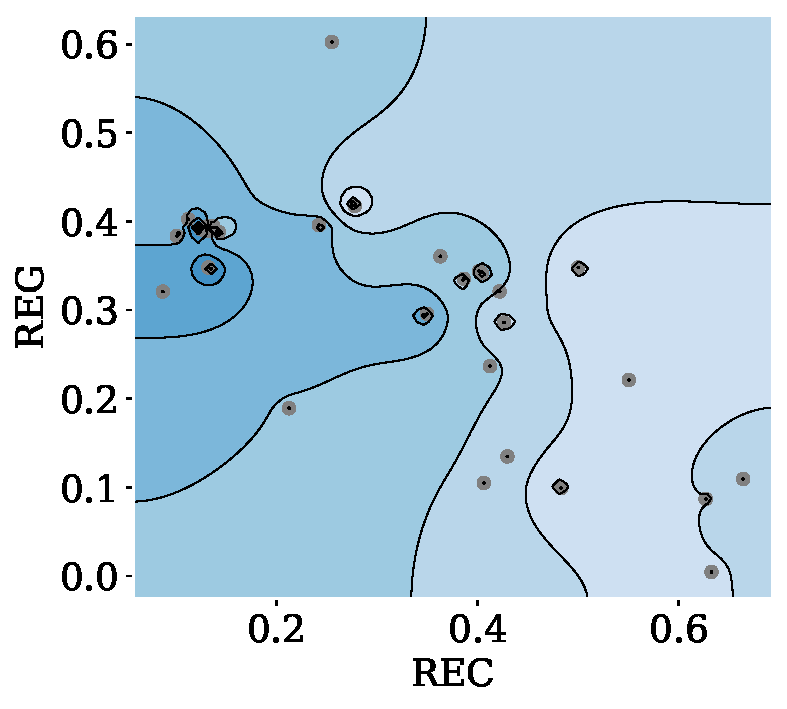
\includegraphics[width=0.34\linewidth,height=3.4cm]{Figures/contour_REC_vs_REG-27.pdf}
}
\subfloat[CLA vs. REG]{%
    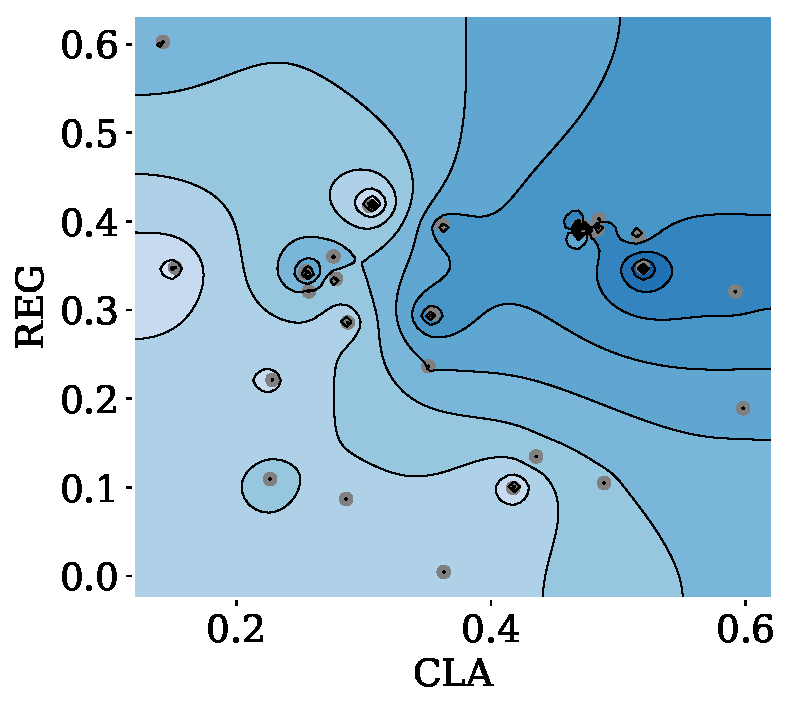
\includegraphics[width=0.34\linewidth,height=3.4cm]{Figures/contour_CLA_vs_REG-27.pdf}
}

\vspace{0.6em}

\begin{tikzpicture}
\begin{axis}[
    hide axis,
    scale only axis,
    width=\linewidth,
    height=0pt,
    colormap name=optunablues,
    colorbar horizontal,
    point meta min=51,
    point meta max=65,
    colorbar style={
        width=\linewidth,
        height=3mm,
        xtick={51, 53, 55, 57, 59, 61, 63, 65},
        xticklabel style={font=\scriptsize},
        xlabel={Val. accuracy (\%)},
        xlabel style={font=\scriptsize, yshift=2pt},
        scaled ticks=false,
        /pgf/number format/fixed,
        /pgf/number format/precision=1,
    },
]
\addplot [draw=none] coordinates {(0,0)};
\end{axis}
\end{tikzpicture}

\end{minipage}%
}

\caption{{Contour plots of validation accuracy (\%) as a function of the normalized loss weights REC, CLA, and REG for Subject~27, a representative subject from the ``Mid'' group on the GigaScience dataset. All panels share the same color scale, allowing direct visual comparison across loss-weight pairs for this subject.}}
\label{fig:global_freq_GIGA27}
\end{figure}
%----------------------------------------------------

{For Subject~27 (Figure~\ref{fig:global_freq_GIGA27}), representative of the ``Mid'' performance group, the validation-accuracy landscape is more heterogeneous than that observed for Subject~14. The lower and more variable accuracy range indicates that this subject is more sensitive to changes in the relative contribution of REC, CLA, and REG. Rather than exhibiting a broad region of stable high performance, the contour maps show more localized regions of improved validation accuracy, suggesting that adequate decoding depends on a more specific loss-weight configuration. This supports the idea that, under less discriminative EEG conditions, the model benefits from a stronger balance between faithful reconstruction and latent-space regularization to stabilize the learned representation~\cite{lotte2018review,saha2020intra}. This behavior agrees with Figure~\ref{fig:distributions}, where the ``Mid'' group shows a reduction in the CLA mode and a relative increase in REC and REG contributions.}

{After analyzing the loss-weight behavior at both the group level and in two representative subjects, we extended the analysis to the complete GigaScience dataset. For this purpose, the hyperparameter search records across all subjects were aggregated and analyzed using a global parameter-importance approach. This analysis estimates how much each optimized loss component contributed to explaining variations in validation accuracy across the full search space. Therefore, while Figures~\ref{fig:distributions},~\ref{fig:global_freq_GIGA14}, and~\ref{fig:global_freq_GIGA27} describe how the loss weights behave across groups and individual subjects, Figure~\ref{fig:GIGA_NRVAE} provides a population-level summary of the relative relevance of REC, CLA, and REG.}

\begin{figure}
    \centering
    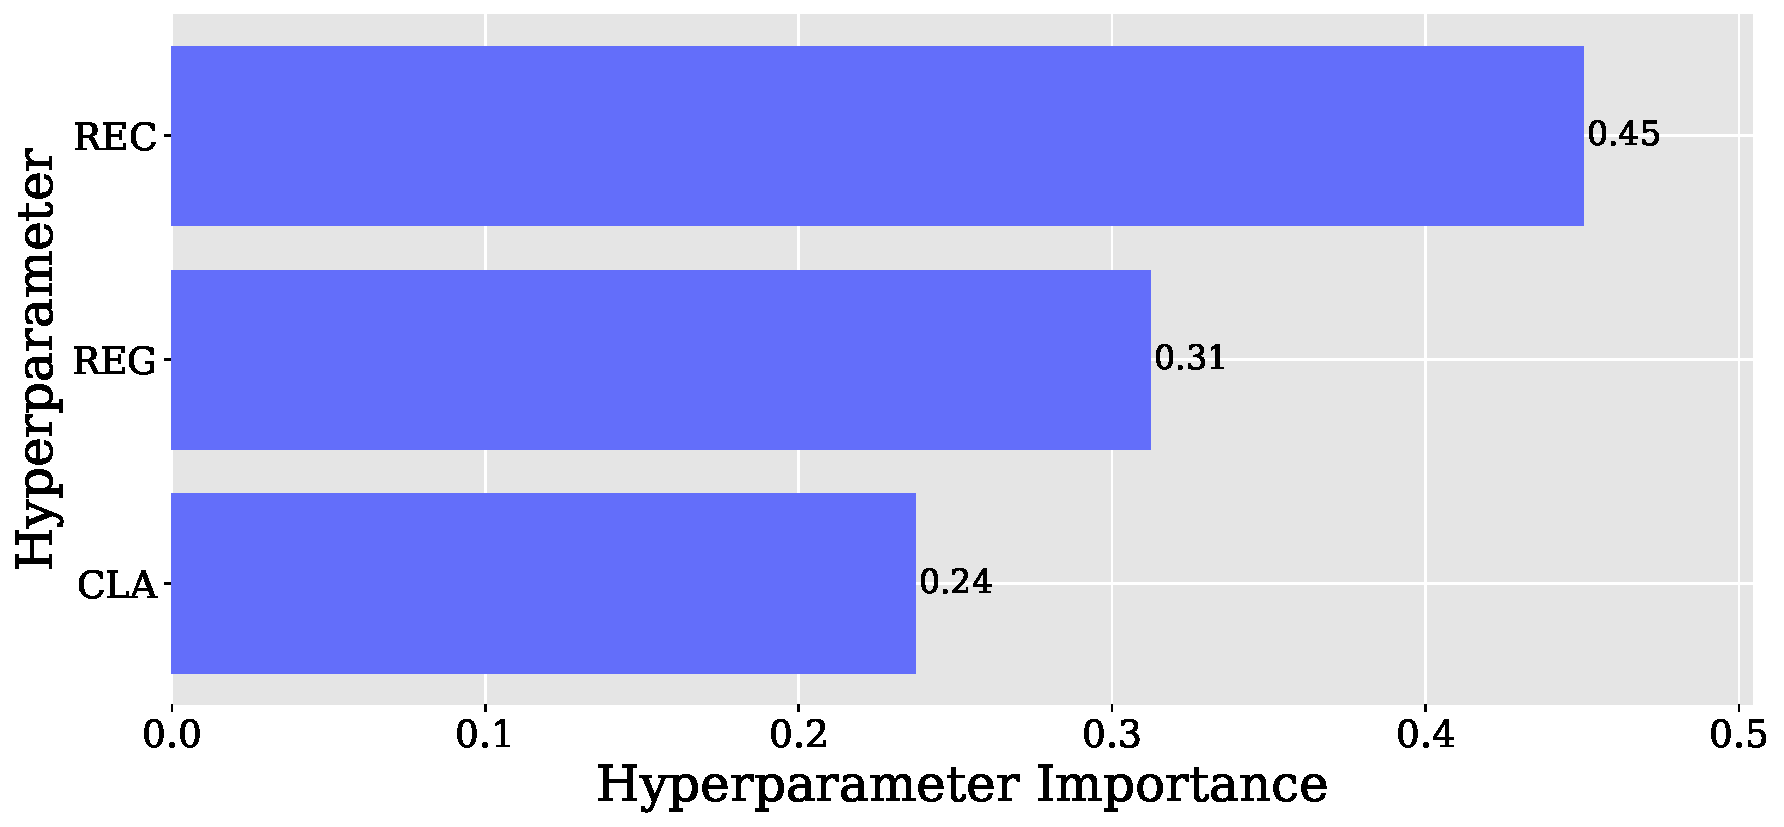
\includegraphics[width=0.8\linewidth]{Figures/optuna_fanova_param_importances_custom.pdf}
    \caption{{Global hyperparameter importance obtained from the Keras Tuner search history for the NRVAE loss-weight configuration across all GigaScience subjects. The importance scores quantify the relative contribution of REC, REG, and CLA to validation accuracy.}}
\label{fig:GIGA_NRVAE}
\end{figure}
%----------------------------------------------------
{The global importance analysis in Figure~\ref{fig:GIGA_NRVAE} shows that REC is the most influential loss-weight hyperparameter, with an importance score of $0.45$, followed by REG ($0.31$) and CLA ($0.24$). This result reinforces the interpretation that \gls{eeggcirnet} does not rely exclusively on direct discriminative optimization. Instead, validation performance across the GigaScience dataset is primarily shaped by the model's ability to preserve a faithful reconstruction of the input connectivity representation, while latent-space regularization provides an additional stabilizing effect~\cite{10483787,Dhanushkodi}. The lower, but still relevant, contribution of CLA indicates that classification remains necessary, but its effectiveness depends on the quality and stability of the learned representation. This finding is consistent with the previous group-level analysis, where the ``Mid'' group showed a reduction in CLA and a relative increase in REC and REG, suggesting that representation learning plays a central role in maintaining performance under more challenging EEG conditions, where inter-subject variability and nonstationarity commonly affect generalization~\cite{lotte2018review,saha2020intra}.}

%---------------------------------------------------
\begin{table}[H]
    \centering
    \caption{Subject-wise Bayesian-optimized loss weights and validation accuracy for \gls{eeggcirnet} on the BCI Competition IV-2a dataset, sorted according to validation performance.}
    \label{tab:bci2a_eegcirnet_hps}
    \begin{tabularx}{\textwidth}{CCCCC}
        \toprule
        \textbf{Subject} & \textbf{REC} & \textbf{CLA} & \textbf{REG} & \textbf{ACC [\%]} \\
        \midrule
        9 & $0.1074$ & $0.2713$ & $0.6213$ & $100.00$ \\
        
        8 & $0.2097$ & $0.2803$ & $0.5100$ & $100.00$ \\
        
        1 & $0.8701$ & $0.0636$ & $0.0663$ & $92.86$ \\
        
        3 & $0.4084$ & $0.0604$ & $0.5312$ & $91.07$ \\
        
        6 & $0.3381$ & $0.3358$ & $0.3261$ & $89.13$ \\
        
        7 & $0.0010$ & $0.5547$ & $0.4442$ & $83.33$ \\
        
        4 & $0.1464$ & $0.4641$ & $0.3895$ & $82.69$ \\
        
        5 & $0.1528$ & $0.3384$ & $0.5088$ & $80.77$ \\
        
        2 & $0.2166$ & $0.3495$ & $0.4340$ & $73.21$ \\
        \midrule
        \textbf{Average} &  & & & $\mathbf{88.56}$ \\
        \bottomrule
    \end{tabularx}
\end{table}
%---------------------------------------------------

%bci 2a 2 class
A complementary perspective on this adaptive behavior is observed in the canonical binary scenario of the BCI Competition IV-2a dataset, summarized in Table~\ref{tab:bci2a_eegcirnet_hps}. Unlike the multi-class \gls{eegmmidb} task or the subject-group validation protocol used for the \gls{adhd}/control dataset, this setting provides a more controlled and well-structured environment in which inter-class separability is generally higher and decision boundaries are more stable. Even under these favorable conditions, \gls{eeggcirnet} does not converge to a single fixed optimization regime, but instead exhibits subject-specific reweighting strategies that reflect the heterogeneity of neural patterns across individuals, a persistent challenge in \gls{eeg}-based \gls{bci} systems~\cite{lotte2018review,saha2020intra}.

For the highest-performing subjects (e.g., Subjects~8 and~9), the optimization converges toward a dominant regularization regime, with the latent regularization (REG) term exceeding $0.50$ and classification weights remaining moderate. This behavior indicates that, when discriminative patterns are highly consistent, enforcing a well-structured latent space becomes sufficient to sustain near-perfect classification performance, effectively stabilizing the learned representations without overemphasizing the discriminative loss. This interpretation is consistent with previous evidence indicating that latent-space regularization can improve robustness and reduce performance degradation in deep \gls{eeg} decoding models~\cite{10483787,Dhanushkodi}.

A more nuanced behavior emerges for subjects with high but non-saturated performance, confirming the presence of distinct subject-specific optimization strategies. Subject~1 exhibits a reconstruction-dominated regime, with REC receiving a markedly high weight ($0.8701$), while CLA and REG remain weakly weighted. This configuration suggests that, for this subject, accurate signal reconstruction plays a central role in preserving and structuring the \gls{eeg} representation prior to classification, in line with generative representation-learning approaches that use reconstruction to promote robust feature encoding~\cite{Dhanushkodi}. Subject~3 follows a hybrid strategy in which regularization and reconstruction dominate (REG $=0.5312$, REC $=0.4084$), while the classification component is strongly downweighted (CLA $=0.0604$). This indicates that stabilizing the latent structure is more critical than direct discriminative pressure for this individual. In contrast, Subject~6 displays a nearly uniform allocation across REC, CLA, and REG (REC $=0.3381$, CLA $=0.3358$, REG $=0.3261$), reflecting a balanced multi-objective optimization regime in which reconstruction fidelity, discriminative supervision, and latent stability jointly contribute to robust decoding.

For the remaining subjects with lower relative validation performance (e.g., Subjects~2,~4,~5, and~7), the optimization shifts toward increased emphasis on classification and latent regularization, with REC receiving comparatively less weight. This pattern suggests that, when signal quality or class separability is reduced, \gls{eeggcirnet} prioritizes strengthening discriminative supervision while simultaneously constraining the latent space to prevent overfitting. Such behavior mirrors the adaptive strategies observed in the ``Mid'' performance group of the GigaScience dataset and in more challenging subjects from the \gls{eegmmidb} collection, reinforcing the interpretation that reconstruction-driven representation learning and regularization act as complementary stabilizing mechanisms when discriminative cues alone are insufficient~\cite{10483787,Dhanushkodi}.

%----------contours---------------
{To further support this subject-specific interpretation, we analyzed the validation-accuracy landscapes obtained from the normalized loss-weight search for two representative cases of the BCI Competition IV-2a dataset: Subject~9, corresponding to the highest-performing subject, and Subject~2, corresponding to the lowest-performing subject. This comparison allows us to examine how the optimization landscape changes between a favorable decoding scenario and a more challenging subject-specific condition. The contour plots in Figures~\ref{fig:global_freq_9} and~\ref{fig:global_freq_2} show pairwise projections of the validation accuracy as a function of REC, CLA, and REG.}

%----------------------------------------------------
\begin{figure}[H]
\centering

\makebox[\textwidth][c]{%
\begin{minipage}[c]{0.99\textwidth}
\centering

\subfloat[REC vs. CLA]{%
    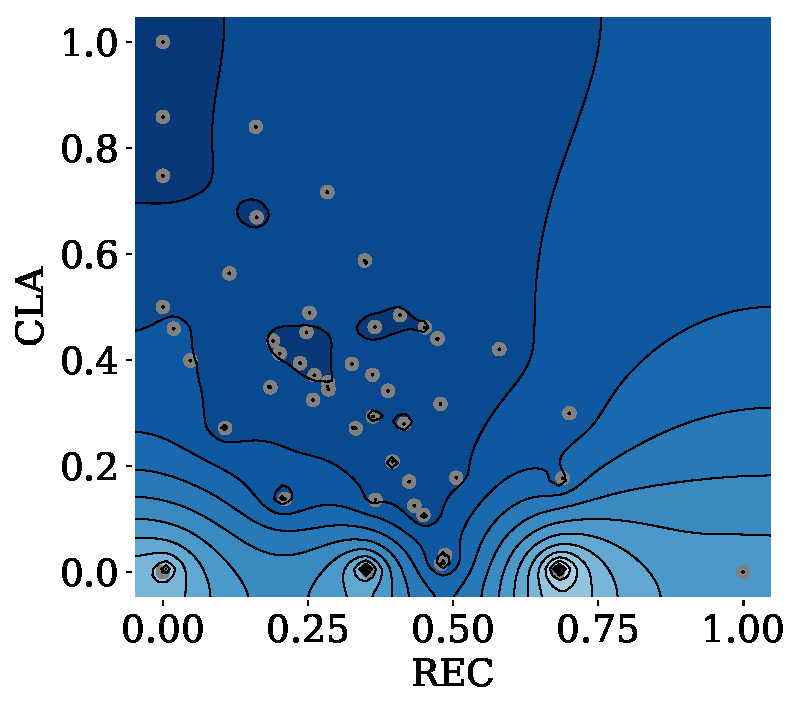
\includegraphics[width=0.34\linewidth,height=3.4cm]{Figures/contour_REC_vs_CLA-9.pdf}
}
\subfloat[REC vs. REG]{%
    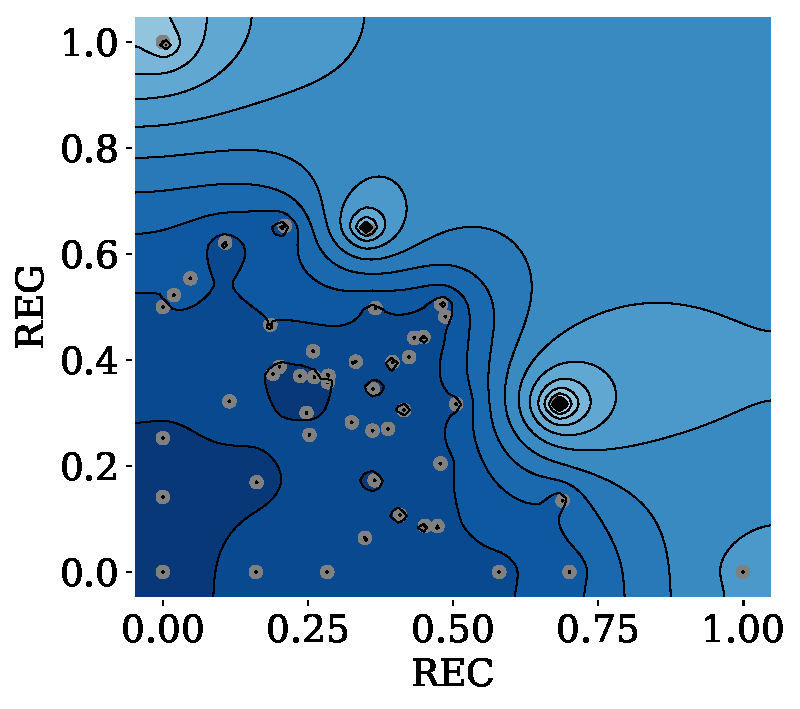
\includegraphics[width=0.34\linewidth,height=3.4cm]{Figures/contour_REC_vs_REG-9.pdf}
}
\subfloat[CLA vs. REG]{%
    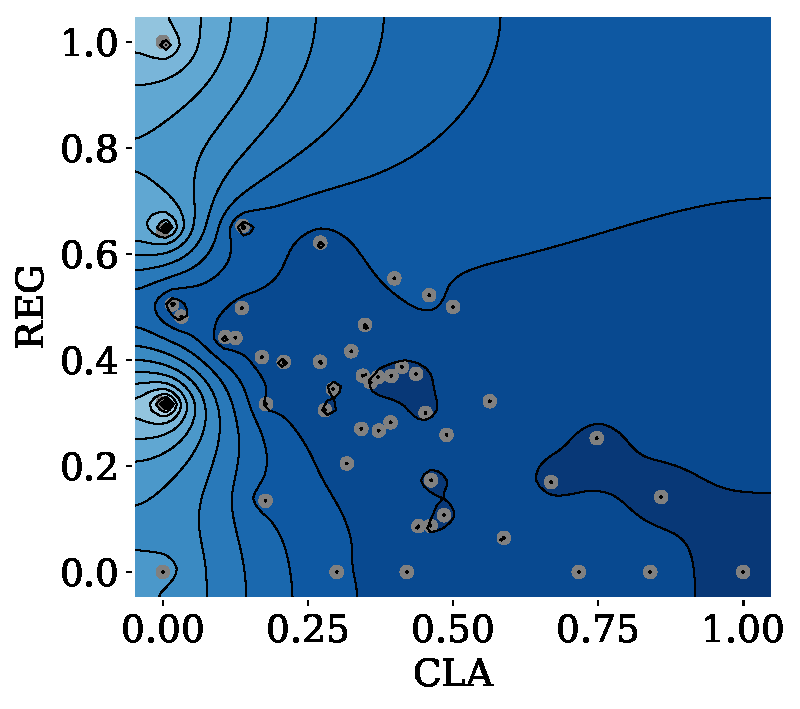
\includegraphics[width=0.34\linewidth,height=3.4cm]{Figures/contour_CLA_vs_REG-9.pdf}
}

\vspace{0.6em}

\begin{tikzpicture}
\begin{axis}[
    hide axis,
    scale only axis,
    width=\linewidth,
    height=0pt,
    colormap name=optunablues,
    colorbar horizontal,
    point meta min=54,
    point meta max=100,
    colorbar style={
        width=\linewidth,
        height=3mm,
        xtick={54, 60, 66, 72, 78, 84, 90, 96, 100},
        xticklabel style={font=\scriptsize},
        xlabel={Val. accuracy (\%)},
        xlabel style={font=\scriptsize, yshift=2pt},
        scaled ticks=false,
        /pgf/number format/fixed,
        /pgf/number format/precision=1,
    },
]
\addplot [draw=none] coordinates {(0,0)};
\end{axis}
\end{tikzpicture}

\end{minipage}%
}

\caption{{Contour plots of validation accuracy (\%) as a function of the normalized loss weights REC, CLA, and REG for Subject~9, the highest-performing subject on the BCI Competition IV-2a dataset. All panels share the same color scale, allowing direct visual comparison across loss-weight pairs for this subject.}}
\label{fig:global_freq_9}
\end{figure}

%----------------------------------------------------
{For Subject~9 (Figure~\ref{fig:global_freq_9}), the contour maps show extended high-performance regions across the explored loss-weight space. This behavior indicates that, for this highly discriminative subject, \gls{eeggcirnet} is relatively robust to moderate variations in the balance among REC, CLA, and REG. In particular, the validation landscape suggests that high accuracy can be preserved across several configurations, provided that the latent representation remains sufficiently structured and the classification term maintains a non-negligible contribution. This agrees with the optimized weights reported in Table~\ref{tab:bci2a_eegcirnet_hps}, where Subject~9 achieves $100\%$ validation accuracy with a REG-dominated configuration. Therefore, in favorable decoding conditions, latent-space regularization appears to act as a stabilizing mechanism that supports near-perfect performance without requiring an excessively dominant classification loss~\cite{10483787,Dhanushkodi}.}

%--------------------------------
\begin{figure}[H]
\centering

\makebox[\textwidth][c]{%
\begin{minipage}[c]{0.99\textwidth}
\centering

\subfloat[REC vs. CLA]{%
    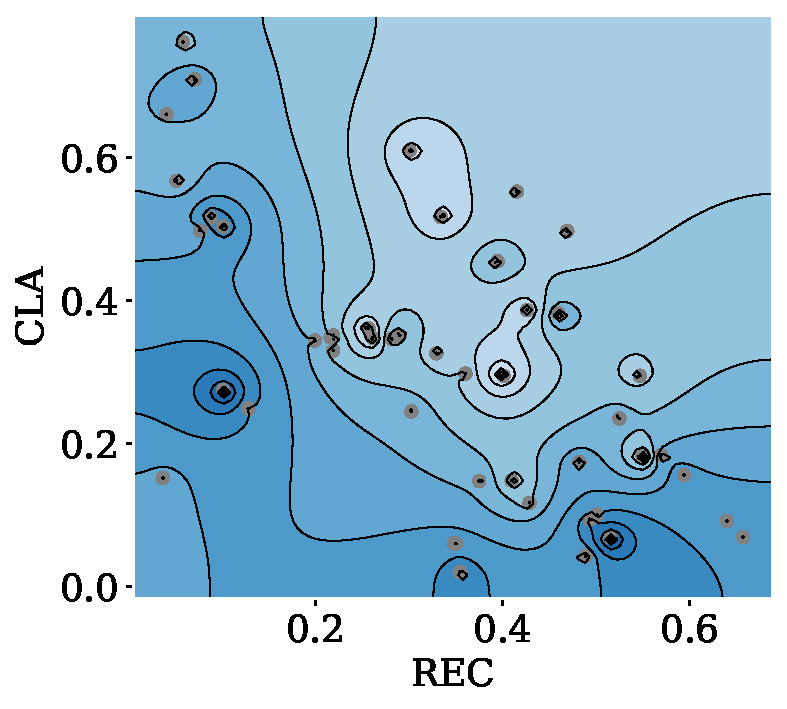
\includegraphics[width=0.34\linewidth,height=3.4cm]{Figures/contour_REC_vs_CLA-2.pdf}
}
\subfloat[REC vs. REG]{%
    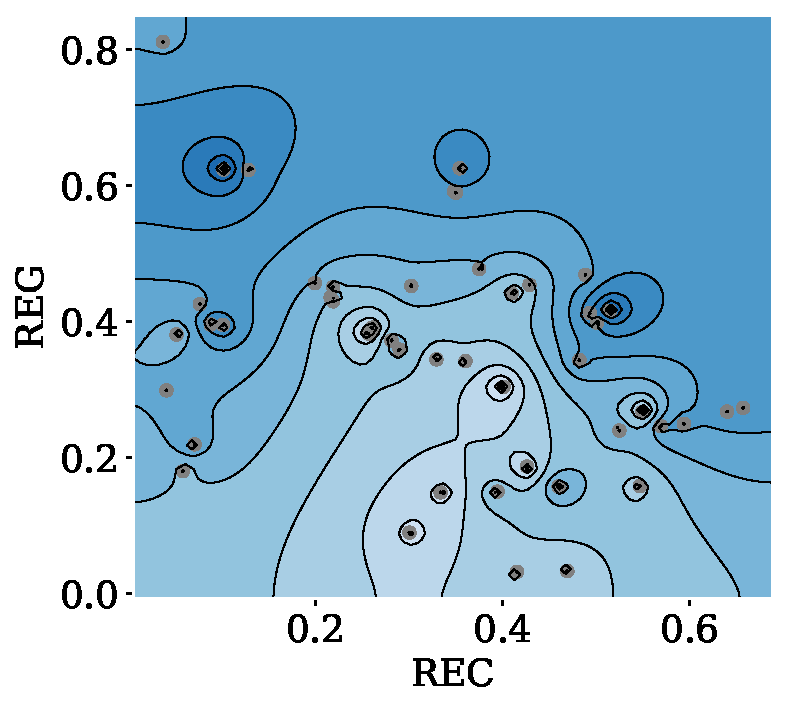
\includegraphics[width=0.34\linewidth,height=3.4cm]{Figures/contour_REC_vs_REG-2.pdf}
}
\subfloat[CLA vs. REG]{%
    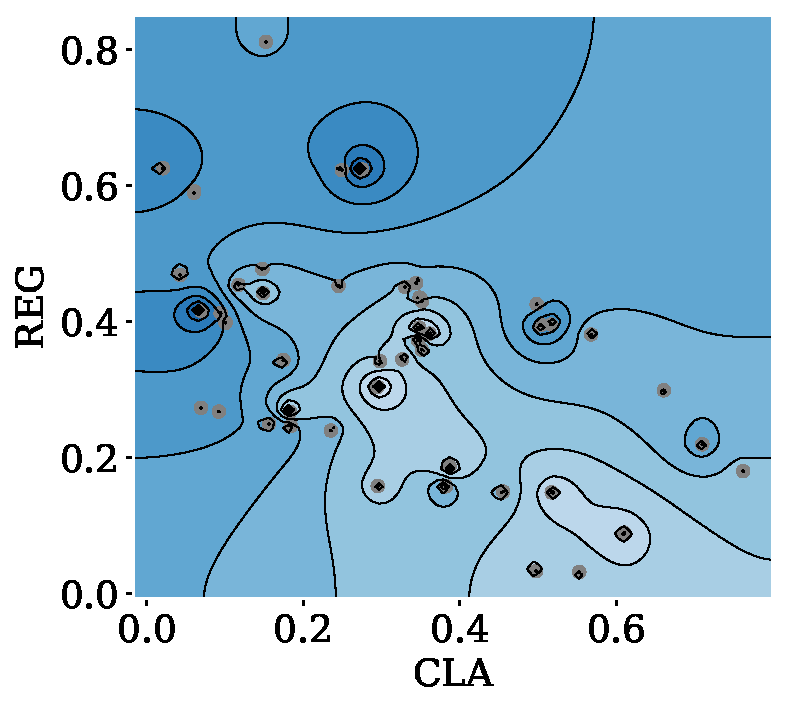
\includegraphics[width=0.34\linewidth,height=3.4cm]{Figures/contour_CLA_vs_REG-2.pdf}
}

\vspace{0.6em}

\begin{tikzpicture}
\begin{axis}[
    hide axis,
    scale only axis,
    width=\linewidth,
    height=0pt,
    colormap name=optunablues,
    colorbar horizontal,
    point meta min=58,
    point meta max=74,
    colorbar style={
        width=\linewidth,
        height=3mm,
        xtick={58, 60, 62, 64, 66, 68, 70, 72, 74},
        xticklabel style={font=\scriptsize},
        xlabel={Val. accuracy (\%)},
        xlabel style={font=\scriptsize, yshift=2pt},
        scaled ticks=false,
        /pgf/number format/fixed,
        /pgf/number format/precision=1,
    },
]
\addplot [draw=none] coordinates {(0,0)};
\end{axis}
\end{tikzpicture}

\end{minipage}%
}

\caption{{Contour plots of validation accuracy (\%) as a function of the normalized loss weights REC, CLA, and REG for Subject~2, the lowest-performing subject on the BCI Competition IV-2a dataset. All panels share the same color scale, allowing direct visual comparison across loss-weight pairs for this subject.}}
\label{fig:global_freq_2}
\end{figure}

%-------------------------------------------------------
{For Subject~2 (Figure~\ref{fig:global_freq_2}), which corresponds to the lowest-performing subject in the BCI Competition IV-2a analysis, the validation-accuracy landscape is more restricted and heterogeneous than that observed for Subject~9. The lower accuracy range and the presence of localized high-performance regions indicate that this subject is more sensitive to the precise balance among REC, CLA, and REG. In particular, the contour maps suggest that improved validation performance is not achieved across broad regions of the search space, but rather within narrower configurations where discriminative supervision and latent-space regularization remain sufficiently emphasized. This interpretation is consistent with the optimized weights reported in Table~\ref{tab:bci2a_eegcirnet_hps}, where Subject~2 reaches its best performance with a combined contribution of REG ($0.4340$) and CLA ($0.3495$), while REC receives a comparatively lower weight ($0.2166$). These results suggest that, under more challenging subject-specific conditions, \gls{eeggcirnet} relies more strongly on classification guidance and latent-space constraints to stabilize the learned representation and prevent performance degradation. This behavior is consistent with the known impact of inter-subject variability on \gls{eeg}-based \gls{bci} generalization~\cite{lotte2018review,saha2020intra}.}

{After examining the subject-specific contour maps, we performed a global hyperparameter-importance analysis across all subjects of the BCI Competition IV-2a dataset. This analysis summarizes the relative contribution of the reconstruction (REC), classification (CLA), and latent-space regularization (REG) weights to validation accuracy, providing a dataset-level view of which loss components most strongly influenced the optimization of \gls{eeggcirnet}.}
%-------------------------------------------------------

\begin{figure}[H]
    \centering
    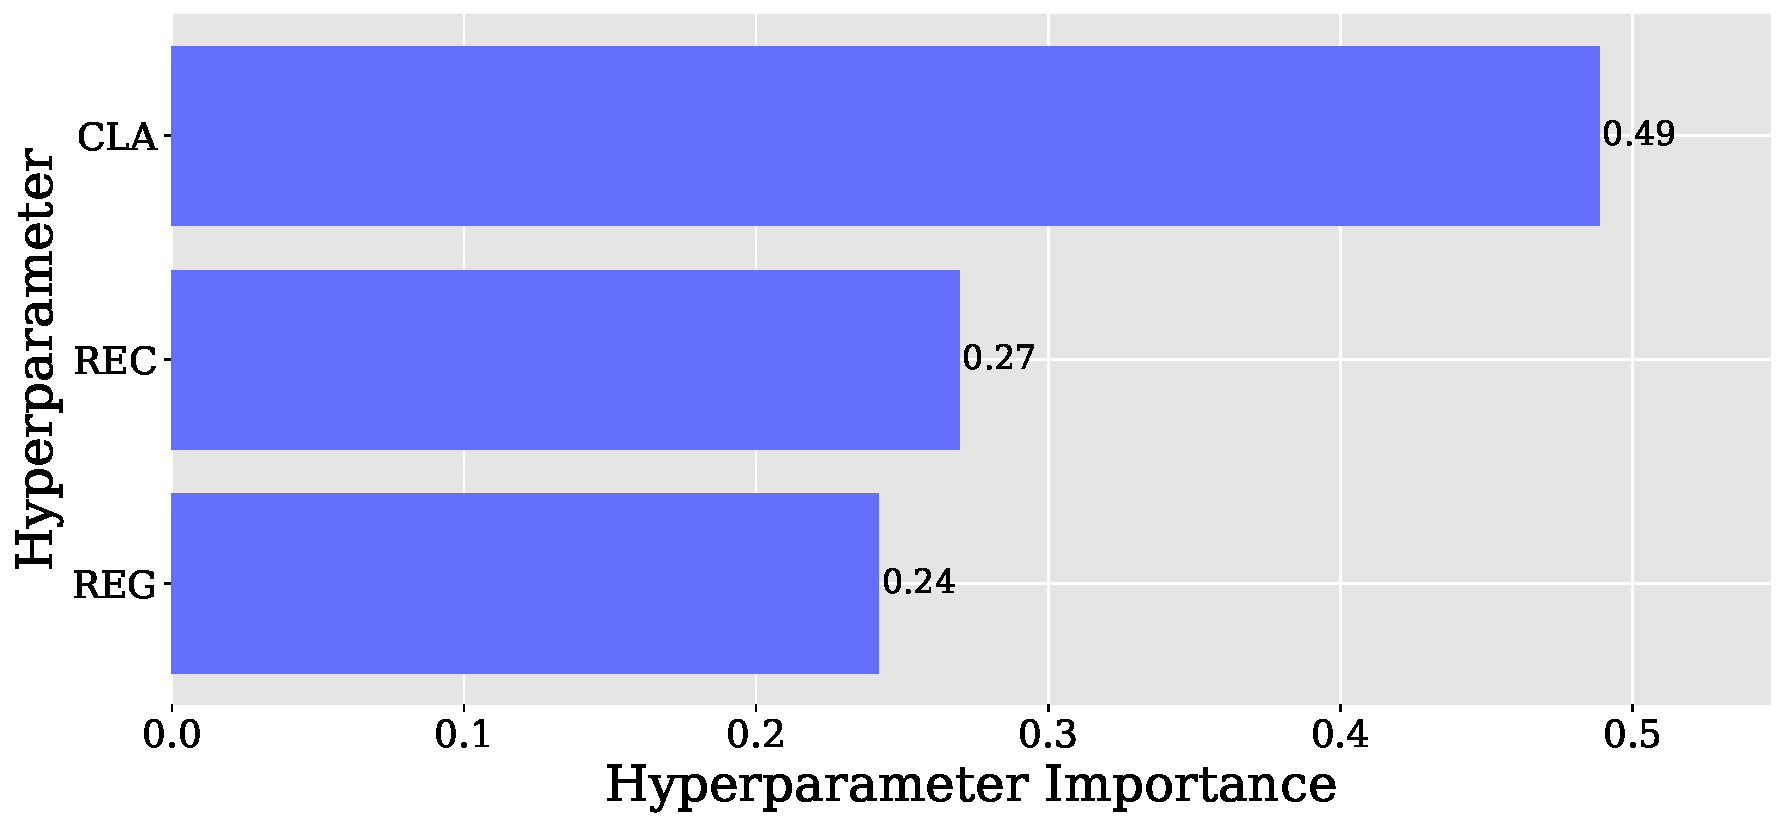
\includegraphics[width=0.8\linewidth]{Figures/optuna_fanova_param_importances_BCI2A-_NRVAE.pdf}
    \caption{{Global hyperparameter importance of the optimized \gls{eeggcirnet} loss weights on the BCI Competition IV-2a dataset. The importance scores quantify the relative contribution of reconstruction (REC), classification (CLA), and latent-space regularization (REG) weights to validation accuracy.}}
    \label{fig:bci2a_fanova_importance}
\end{figure}

%-------------------------------------------------------

{The global importance analysis in Figure~\ref{fig:bci2a_fanova_importance} shows that CLA is the most influential loss-weight hyperparameter in the BCI Competition IV-2a scenario, with an importance score of $0.49$, followed by REC ($0.27$) and REG ($0.24$). This result contrasts with the GigaScience analysis, where REC had the largest global contribution, and suggests that the canonical binary BCI IV-2a setting relies more strongly on direct discriminative supervision. Nevertheless, the non-negligible contributions of REC and REG indicate that classification performance is still supported by representation reconstruction and latent-space stabilization. Therefore, even in a more controlled binary decoding task, \gls{eeggcirnet} benefits from a multi-objective optimization strategy rather than relying exclusively on the classification loss. This finding reinforces the role of adaptive loss-weight reorganization as a mechanism for balancing discriminative learning with representation stability under subject-specific \gls{eeg} variability~\cite{lotte2018review,saha2020intra,Dhanushkodi}.}

Taken together, the BCI Competition IV-2a results complete the picture established across datasets: \gls{eeggcirnet} does not rely on a fixed balance between reconstruction, classification, and regularization, but dynamically reorganizes its internal optimization priorities according to signal characteristics and task difficulty. This consistency across canonical, multi-class, and subject-group validation scenarios provides strong evidence that the proposed framework internalizes a principled adaptive learning strategy rather than overfitting to any particular experimental condition, addressing a central limitation of \gls{eeg}-based \gls{bci} models under inter-subject variability~\cite{lotte2018review,saha2020intra}.

%----------------------------------------------------
%%aqui quedeeeeeeeee
%----------------------------------------------------

%physionet
\begin{table}[H]
    \centering
    \caption{Subject-specific weight distribution for reconstruction (REC), classification (CLA), latent regularization (REG), and mean accuracy across the selected subjects of the \gls{eegmmidb} dataset.}
    \label{tab:weights_dist}
    \begin{tabularx}{\textwidth}{CCCCC}
        \toprule
        \textbf{Subject} & \textbf{REC} & \textbf{CLA} & \textbf{REG} & \textbf{ACC [\%]} \\
        \midrule
        $13$ & $0.0000$ & $1.0000$ & $0.0000$ & $77.80$ \\
        $50$ & $0.5000$ & $0.5000$ & $0.0000$ & $77.76$ \\
        $12$ & $0.3655$ & $0.6345$ & $0.0000$ & $77.77$ \\
        $9$  & $0.3803$ & $0.6197$ & $0.0000$ & $76.19$ \\
        $40$ & $0.3559$ & $0.6441$ & $0.0000$ & $76.20$ \\
        $7$  & $0.4958$ & $0.3824$ & $0.1219$ & $77.70$ \\
        $41$ & $0.5401$ & $0.4583$ & $0.0017$ & $71.40$ \\
        $49$ & $0.8303$ & $0.1697$ & $0.0000$ & $73.00$ \\
        $3$  & $0.4421$ & $0.4615$ & $0.0964$ & $71.43$ \\
        $8$  & $0.3869$ & $0.4379$ & $0.1753$ & $73.02$ \\
        \midrule
        \textbf{Average} &  &  &  & $\mathbf{75.20}$ \\
        \bottomrule
    \end{tabularx}
\end{table}

%----------------------------------------------------
%physionet multiclass
Likewise, we analyzed the learned loss component weights ($\lambda_{\text{REC}}$, $\lambda_{\text{CLA}}$, $\lambda_{\text{REG}}$) for the multi-class scenario, as detailed in Table~\ref{tab:weights_dist}. The distribution of these weights corroborates the adaptive optimization strategy observed in the binary task, but reveals distinct behaviors necessitated by the increased complexity of the 5-class problem. For the highest-performing subject (Subject 13), the model converges to a purely discriminative state ($\lambda_{\text{CLA}} = 1.0000$, $\lambda_{\text{REC}} = \lambda_{\text{REG}} = 0$), indicating that the spatio-spectral features were sufficiently distinct to drive classification without the need for auxiliary regularization. Conversely, for subjects with moderate performance (e.g., S50, S12, S40), the model adopts a hybrid strategy, balancing classification importance ($\lambda_{\text{CLA}} \approx 0.60$) with reconstruction fidelity ($\lambda_{\text{REC}} \approx 0.40$), while keeping the latent regularization term deactivated ($\lambda_{\text{REG}} = 0$). This suggests that for reasonably separable data, the autoencoder acts primarily as a feature extractor rather than a generative regularizer.

However, a critical shift occurs for the most challenging subjects (e.g., 7, 3, 8), where the baseline methods struggled. Here, the model explicitly activates the latent space regularization ($\lambda_{\text{REG}} > 0.09$), reaching values up to $0.1753$ for Subject 8. This indicates that when decision boundaries are ambiguous, \gls{eeggcirnet} automatically prioritizes the formation of a well-structured Gaussian latent space to prevent overfitting. An extreme case is observed for Subject 49, where the model shifts almost entirely to representation learning ($\lambda_{\text{REC}} = 0.8303$), effectively operating as a non-linear denoiser to stabilize the input features before attempting classification. This evident reorganization of optimization priorities confirms that the architecture is not a static ``black box,'' but an adaptive system that modulates its learning objective based on the difficulty of the underlying \mbox{neural patterns.}

%----------contours EEGMMIDB---------------

{To further support the subject-specific interpretation derived from Table~\ref{tab:weights_dist}, we analyzed the validation-accuracy landscapes for two representative subjects from the multi-class \gls{eegmmidb} scenario: Subject~12, one of the highest-performing subjects, and Subject~41, a moderate-performance subject. This comparison provides a visual characterization of how the optimized balance among reconstruction (REC), classification (CLA), and latent-space regularization (REG) changes as the 5-class decoding problem becomes more challenging. The contour plots in Figures~\ref{fig:global_freq_12} and~\ref{fig:global_freq_Sbj41} show pairwise projections of the validation accuracy over the normalized loss-weight space.}

%----------------------------------------------------
\begin{figure}[htbp]]
\centering

\makebox[\textwidth][c]{%
\begin{minipage}[c]{0.99\textwidth}
\centering

\subfloat[REC vs. CLA]{%
    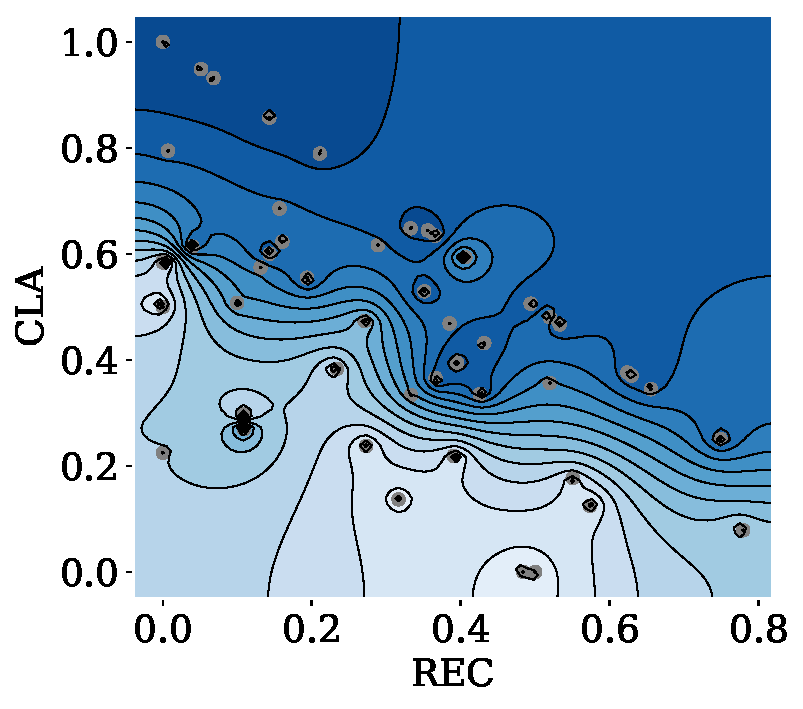
\includegraphics[width=0.34\linewidth,height=3.4cm]{Figures/contour_REC_vs_CLA-12.pdf}
}
\subfloat[REC vs. REG]{%
    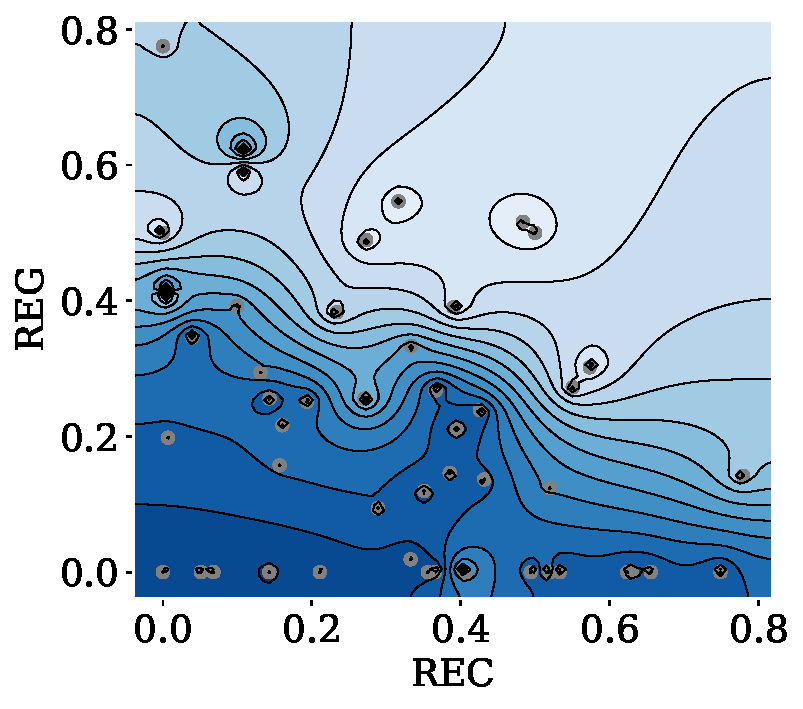
\includegraphics[width=0.34\linewidth,height=3.4cm]{Figures/contour_REC_vs_REG-12.pdf}
}
\subfloat[CLA vs. REG]{%
    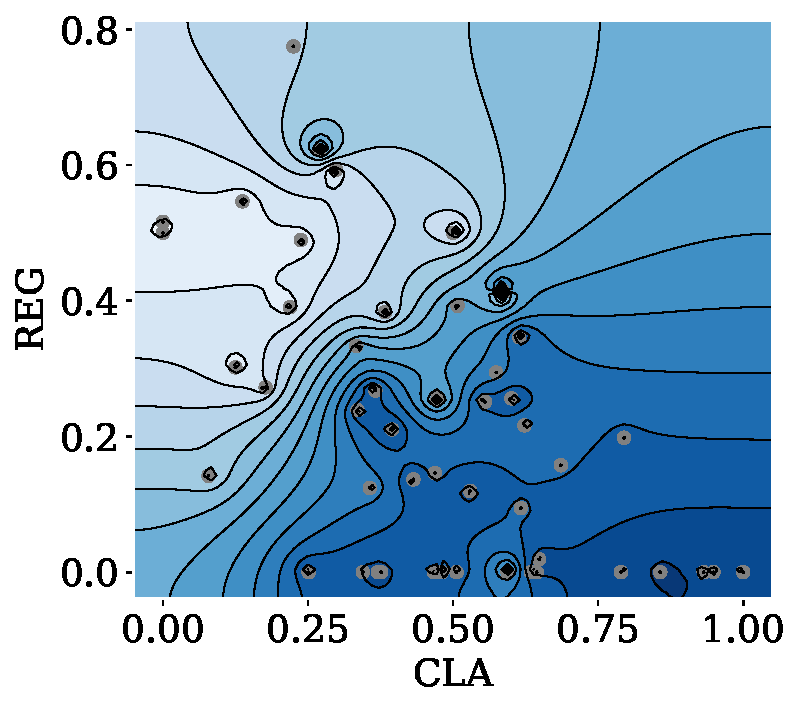
\includegraphics[width=0.34\linewidth,height=3.4cm]{Figures/contour_CLA_vs_REG-12.pdf}
}

\vspace{0.6em}

\begin{tikzpicture}
\begin{axis}[
    hide axis,
    scale only axis,
    width=\linewidth,
    height=0pt,
    colormap name=optunablues,
    colorbar horizontal,
    point meta min=20,
    point meta max=77,
    colorbar style={
        width=\linewidth,
        height=3mm,
        xtick={20, 28, 36, 44, 52, 60, 68, 77},
        xticklabel style={font=\scriptsize},
        xlabel={Val. accuracy (\%)},
        xlabel style={font=\scriptsize, yshift=2pt},
        scaled ticks=false,
        /pgf/number format/fixed,
        /pgf/number format/precision=1,
    },
]
\addplot [draw=none] coordinates {(0,0)};
\end{axis}
\end{tikzpicture}

\end{minipage}%
}

\caption{{Contour plots of validation accuracy (\%) as a function of the normalized loss weights REC, CLA, and REG for Subject~12, one of the highest-performing subjects in the \gls{eegmmidb} multi-class scenario. All panels share the same color scale, allowing direct visual comparison across loss-weight pairs for this subject.}}
\label{fig:global_freq_12}
\end{figure}
%----------------------------------------------------

{For Subject~12 (Figure~\ref{fig:global_freq_12}), the validation landscape shows extended high-performance regions mainly associated with a strong classification contribution and low latent regularization. This behavior agrees with the optimized weights reported in Table~\ref{tab:weights_dist}, where Subject~12 achieves high accuracy with a CLA-dominant configuration ($\lambda_{\text{CLA}}=0.6345$), a relevant reconstruction contribution ($\lambda_{\text{REC}}=0.3655$), and inactive regularization ($\lambda_{\text{REG}}=0$). Thus, for this favorable multi-class case, direct discriminative supervision appears to be the main optimization driver, while reconstruction still contributes to preserving a stable connectivity-based representation, consistent with representation-learning strategies where reconstruction supports robust feature encoding~\cite{Dhanushkodi}.}

%----------------------------------------------------
\begin{figure}[htbp]]
\centering

\makebox[\textwidth][c]{%
\begin{minipage}[c]{0.99\textwidth}
\centering

\subfloat[REC vs. CLA]{%
    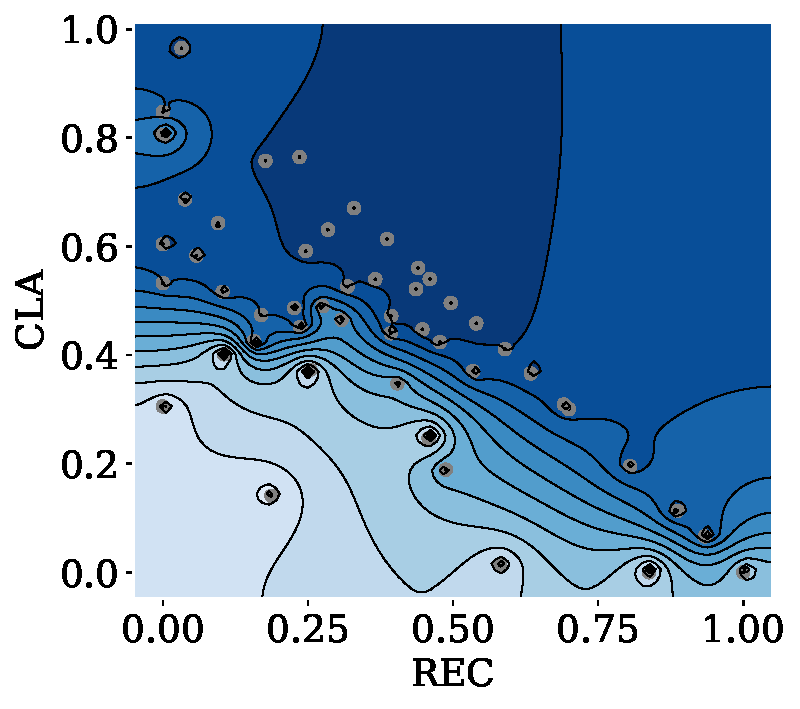
\includegraphics[width=0.34\linewidth,height=3.4cm]{Figures/contour_REC_vs_CLA-41.pdf}
}
\subfloat[REC vs. REG]{%
    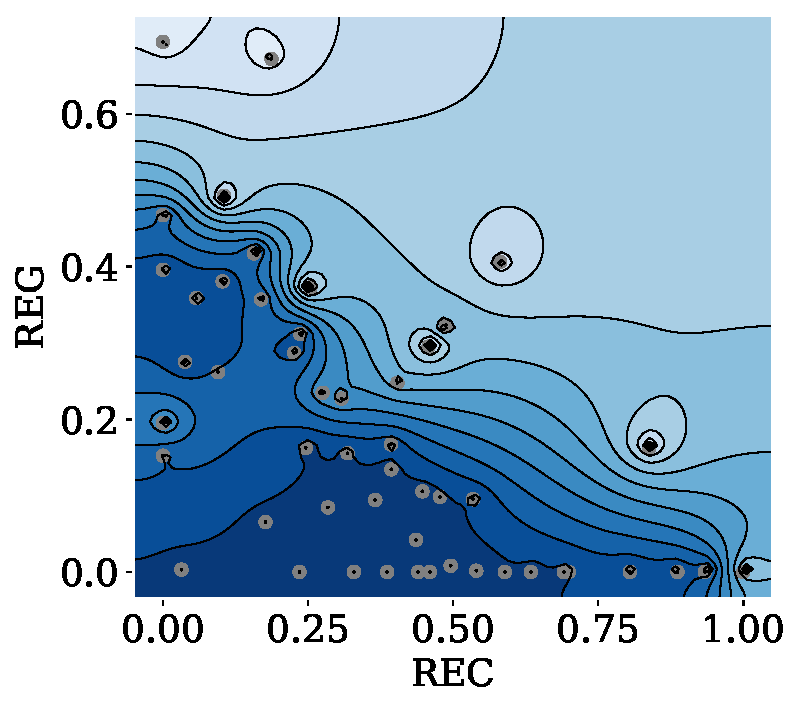
\includegraphics[width=0.34\linewidth,height=3.4cm]{Figures/contour_REC_vs_REG-41.pdf}
}
\subfloat[CLA vs. REG]{%
    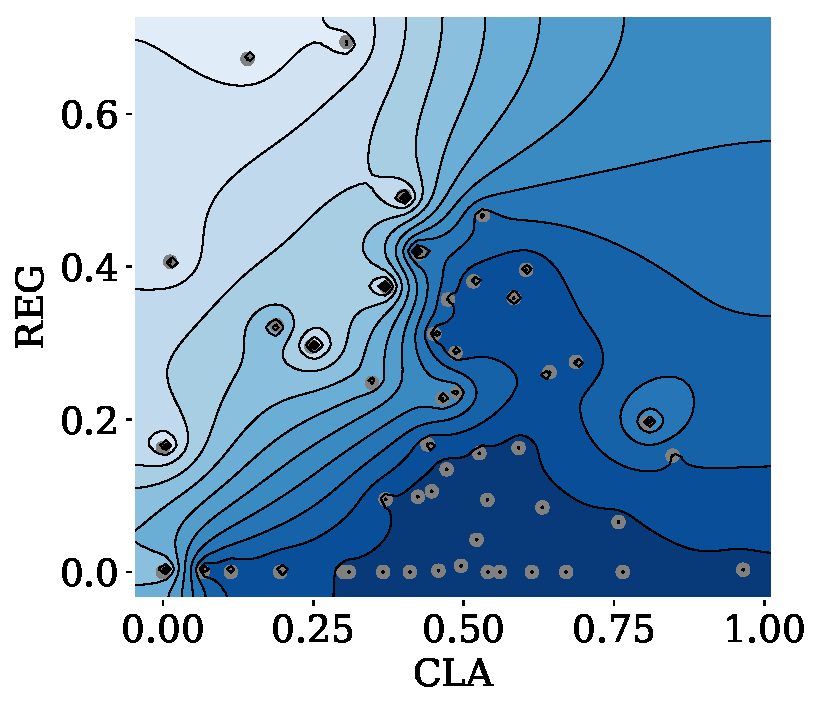
\includegraphics[width=0.34\linewidth,height=3.4cm]{Figures/contour_CLA_vs_REG-41.pdf}
}

\vspace{0.6em}

\begin{tikzpicture}
\begin{axis}[
    hide axis,
    scale only axis,
    width=\linewidth,
    height=0pt,
    colormap name=optunablues,
    colorbar horizontal,
    point meta min=20,
    point meta max=68,
    colorbar style={
        width=\linewidth,
        height=3mm,
        xtick={20, 28, 36, 44, 52, 60, 68},
        xticklabel style={font=\scriptsize},
        xlabel={Val. accuracy (\%)},
        xlabel style={font=\scriptsize, yshift=2pt},
        scaled ticks=false,
        /pgf/number format/fixed,
        /pgf/number format/precision=1,
    },
]
\addplot [draw=none] coordinates {(0,0)};
\end{axis}
\end{tikzpicture}

\end{minipage}%
}

\caption{{Contour plots of validation accuracy (\%) as a function of the normalized loss weights REC, CLA, and REG for Subject~41, a moderate-performance subject in the \gls{eegmmidb} multi-class scenario. All panels share the same color scale, allowing direct visual comparison across loss-weight pairs for this subject.}}
\label{fig:global_freq_Sbj41}
\end{figure}
%---------------------------------------------------

{For Subject~41 (Figure~\ref{fig:global_freq_Sbj41}), the contour maps reveal a more constrained validation landscape, suggesting greater sensitivity to the precise balance between reconstruction and classification. In contrast to Subject~12, the best-performing configuration for Subject~41 relies on a more balanced REC--CLA allocation ($\lambda_{\text{REC}}=0.5401$, $\lambda_{\text{CLA}}=0.4583$), with an almost negligible regularization term ($\lambda_{\text{REG}}=0.0017$). This indicates that, for a more challenging subject, \gls{eeggcirnet} does not simply increase discriminative pressure; instead, it requires a stronger reconstruction component to preserve the structure of the input representation while maintaining sufficient classification guidance. Overall, Figures~\ref{fig:global_freq_12} and~\ref{fig:global_freq_Sbj41} confirm that the multi-class optimization process is not governed by a single dominant configuration. Rather, \gls{eeggcirnet} explores a structured and subject-dependent loss-weight landscape, adapting the relative contribution of REC, CLA, and REG according to the separability and stability of the underlying neural patterns, which is consistent with the known impact of inter-subject variability on \gls{eeg}-based \gls{bci} generalization~\cite{lotte2018review,saha2020intra}.}

%-------------------------------------------------------
{After examining the subject-specific contour maps, we performed a global hyperparameter-importance analysis across all selected subjects of the \gls{eegmmidb} dataset. This analysis provides a dataset-level view of which loss-weight components most strongly influenced validation accuracy in the multi-class scenario.}

\begin{figure}[H]
    \centering
    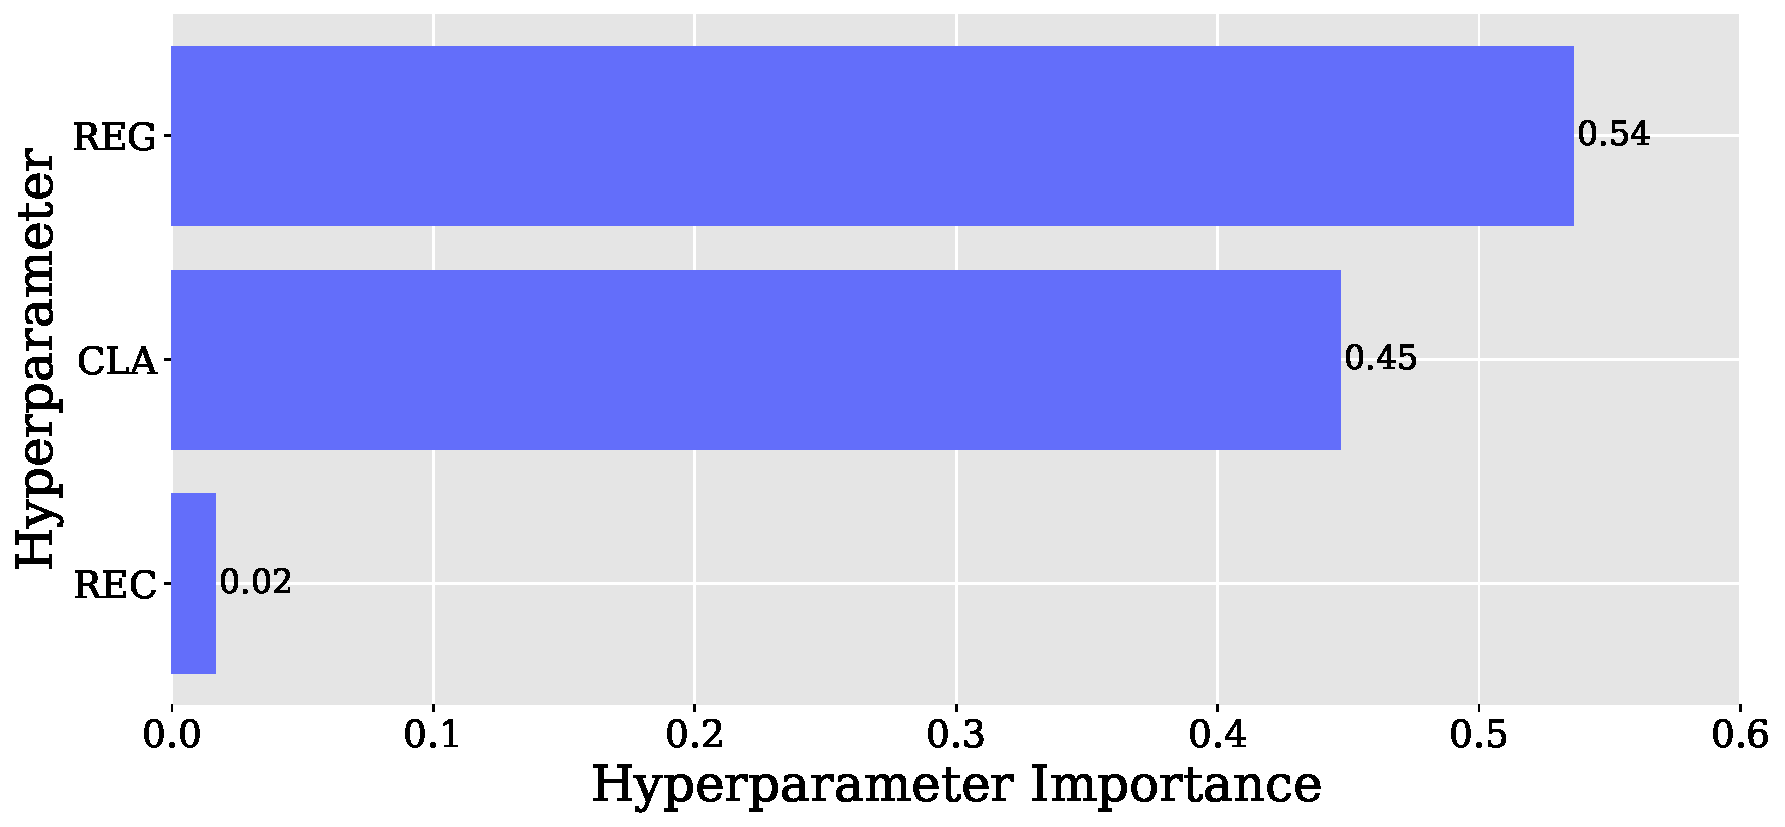
\includegraphics[width=0.8\linewidth]{Figures/optuna_fanova_param_importances_PHY_NRVAE.pdf}
    \caption{{Global hyperparameter importance of the optimized \gls{eeggcirnet} loss weights on the \gls{eegmmidb} dataset. The importance scores quantify the relative contribution of reconstruction (REC), classification (CLA), and latent-space regularization (REG) weights to validation accuracy.}}
    \label{fig:eegmmidb_fanova_importance}
\end{figure}
%-------------------------------------------------------

{The global importance analysis in Figure~\ref{fig:eegmmidb_fanova_importance} shows that REG is the most influential loss-weight hyperparameter in the multi-class \gls{eegmmidb} scenario, with an importance score of $0.54$, followed closely by CLA ($0.45$), while REC shows a markedly lower global contribution ($0.02$). This result suggests that, when the decoding task involves multiple motor imagery and resting-state classes, validation performance is mainly shaped by the interaction between discriminative supervision and latent-space regularization. In this context, REG appears to play a central role in stabilizing the shared latent representation, while CLA remains essential for preserving class-specific separability. The low global importance of REC does not imply that reconstruction is irrelevant; rather, it indicates that its contribution is more subject-specific, as observed in cases such as Subject~41 and Subject~49. Overall, the \gls{eegmmidb} analysis confirms that \gls{eeggcirnet} adapts its optimization priorities according to task complexity, relying more strongly on latent-space regularization and classification guidance in the multi-class setting~\cite{lotte2018review,saha2020intra}.}

%-------------------------------------------------------
TDHA SGKF Under the subject-group validation scheme imposed by the SGKF-CV protocol, \gls{eeggcirnet} achieves a mean accuracy of $63.50\%$ across the five folds on the \gls{adhd}/control children dataset, as reported in Table~\ref{tab:tdha_eegcirnet_hps}. This moderate performance reflects the increased difficulty of the dataset and the strictness of group-wise validation, which prevents subject leakage between training and test partitions. Such a setting is particularly demanding in pediatric \gls{adhd} data, where inter-subject heterogeneity, attentional variability, and subject-dependent neural patterns complicate subject-independent generalization~\cite{lotte2018review,saha2020intra}.

%---------------------------------------------------
\begin{table}[H]
    \centering
    \caption{Bayesian-optimized loss weights and fold-wise accuracy of \gls{eeggcirnet} on the \gls{adhd}/control children dataset under SGKF validation.}
    \label{tab:tdha_eegcirnet_hps}
    \begin{tabularx}{\textwidth}{CCCCC}
        \toprule
        \textbf{Fold} & \textbf{REC} & \textbf{CLA} & \textbf{REG} & \textbf{ACC [\%]} \\
        \midrule
        1 & $0.4443$ & $0.1249$ & $0.4308$ & $66.49$ \\
        
        2 & $0.4802$ & $0.2194$ & $0.3004$ & $57.78$ \\
        
        3 & $0.1272$ & $0.4243$ & $0.4486$ & $63.02$ \\
        
        4 & $0.4501$ & $0.4368$ & $0.1130$ & $62.64$ \\
        
        5 & $0.3554$ & $0.4565$ & $0.1881$ & $67.56$ \\
        \midrule
        \textbf{Average} &  &  &  & $\mathbf{63.50}$ \\
        \bottomrule
    \end{tabularx}
\end{table}
%---------------------------------------------------

The optimized configurations reveal strong fold-wise variability in the allocation of REC, CLA, and REG. Since each SGKF fold contains a different held-out subject group, the fold-wise accuracy should not be interpreted as a direct consequence of a single loss-weight pattern. Instead, Table~\ref{tab:tdha_eegcirnet_hps} shows that \gls{eeggcirnet} adapts its optimization balance according to the specific train--test split. Fold~1 follows a REC--REG-oriented configuration, Fold~2 assigns its largest contribution to REC with additional REG support, Fold~3 shifts toward a CLA--REG strategy, whereas Folds~4 and~5 emphasize REC--CLA with lower REG. This variability indicates that no single loss-weight configuration is uniformly optimal across folds. Importantly, all three components remain active across folds, suggesting that reconstruction fidelity, discriminative supervision, and latent-space regularization jointly contribute to maintaining training stability under strict subject-independent validation.

{To further examine the optimization behavior under the SGKF-CV protocol, we analyzed the validation-accuracy landscape obtained from the hyperparameter search across the five folds. Unlike the previous contour analyses for GigaScience, BCI Competition IV-2a, and \gls{eegmmidb}, this analysis does not correspond to a representative subject, but rather to the global behavior induced by the fold-wise validation scheme. Therefore, the contour plots in Figure~\ref{fig:contour_tdha-EEGCIRNET} summarize how different combinations of the normalized reconstruction (REC), classification (CLA), and latent-space regularization (REG) weights affect validation accuracy across heterogeneous train--test subject splits in the \gls{adhd}/control children dataset.}

%----------------------------------------------------
\begin{figure}[H]
\centering

\makebox[\textwidth][c]{%
\begin{minipage}[c]{0.99\textwidth}
\centering

\subfloat[REC vs. CLA]{%
    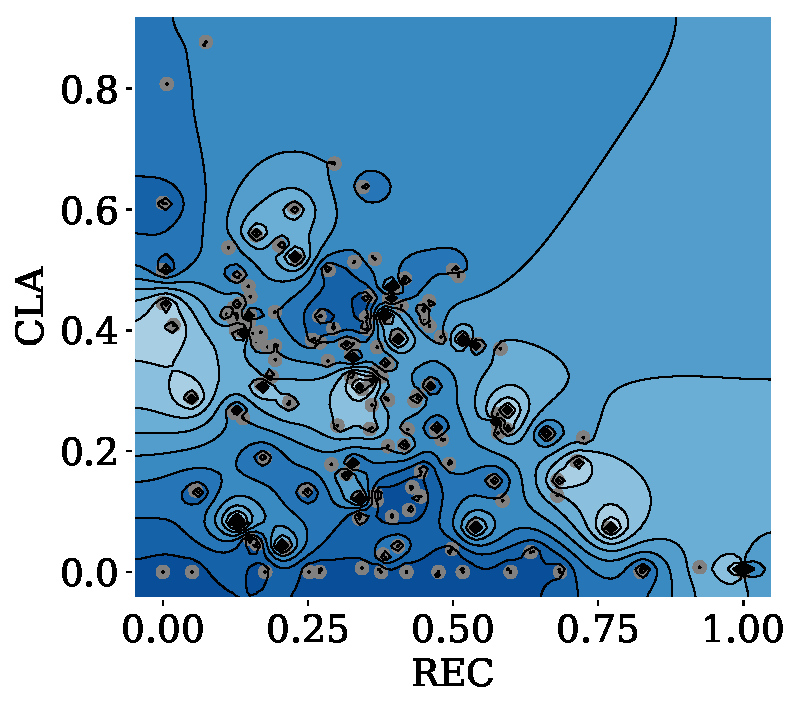
\includegraphics[width=0.34\linewidth,height=3.4cm]{Figures/contour_REC_vs_CLA-adhd.pdf}
}
\subfloat[REC vs. REG]{%
    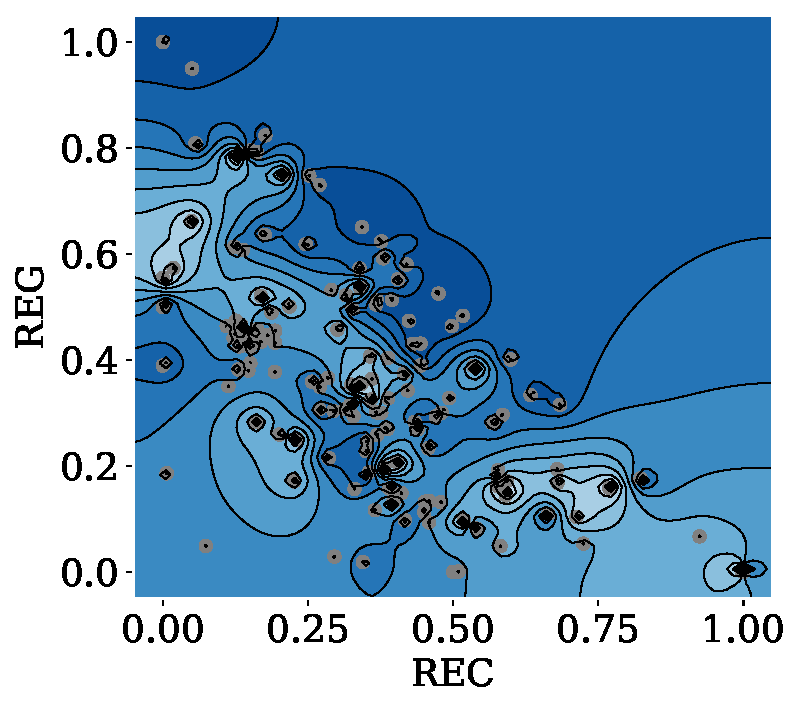
\includegraphics[width=0.34\linewidth,height=3.4cm]{Figures/contour_REC_vs_REG-adhd.pdf}
}
\subfloat[CLA vs. REG]{%
    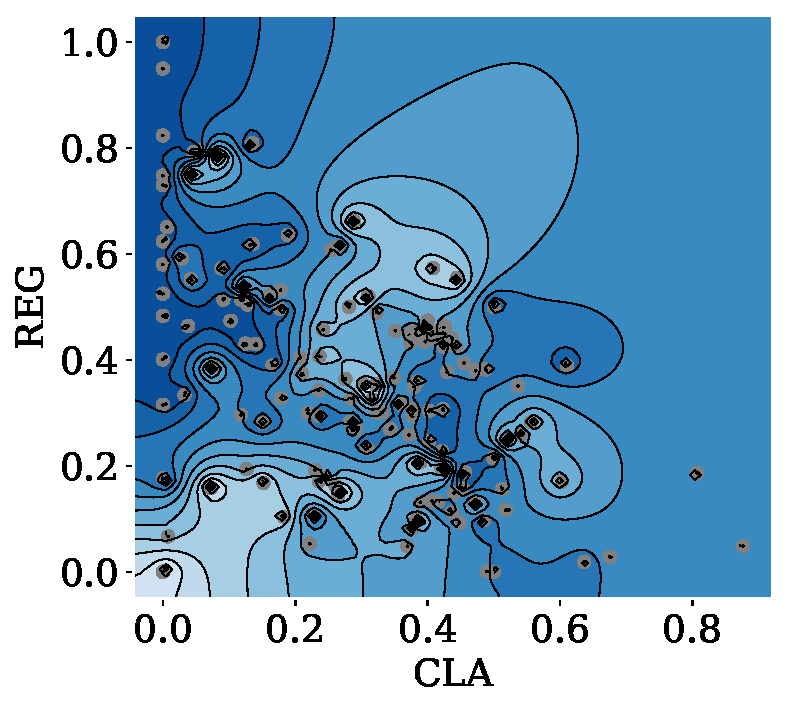
\includegraphics[width=0.34\linewidth,height=3.4cm]{Figures/contour_CLA_vs_REG-adhd.pdf}
}

\vspace{0.6em}

\begin{tikzpicture}
\begin{axis}[
    hide axis,
    scale only axis,
    width=\linewidth,
    height=0pt,
    colormap name=optunablues,
    colorbar horizontal,
    point meta min=42,
    point meta max=66,
    colorbar style={
        width=\linewidth,
        height=3mm,
        xtick={42, 46, 50, 54, 58, 62, 66},
        xticklabel style={font=\scriptsize},
        xlabel={Val. accuracy (\%)},
        xlabel style={font=\scriptsize, yshift=2pt},
        scaled ticks=false,
        /pgf/number format/fixed,
        /pgf/number format/precision=1,
    },
]
\addplot [draw=none] coordinates {(0,0)};
\end{axis}
\end{tikzpicture}

\end{minipage}%
}

\caption{{Contour plots of validation accuracy (\%) as a function of the normalized loss weights REC, CLA, and REG for the \gls{adhd}/control children dataset under the SGKF-CV validation scheme. All panels share the same color scale, allowing direct visual comparison across loss-weight pairs.}}
\label{fig:contour_tdha-EEGCIRNET}
\end{figure}
%----------------------------------------------------

{Figure~\ref{fig:contour_tdha-EEGCIRNET} reveals a highly irregular validation-accuracy landscape for the \gls{adhd}/control children dataset under the SGKF-CV protocol. Unlike the smoother and more structured patterns observed in the BCI-oriented datasets, the contour maps show multiple localized regions of varying performance rather than a single broad optimum. This behavior is particularly evident in the REC--CLA and CLA--REG projections, where regions of improved validation accuracy appear scattered across the loss-weight space, indicating that the model is highly sensitive to small changes in the relative contribution of reconstruction, classification, and latent-space regularization.}

{This fragmented landscape is consistent with the strict nature of SGKF-CV, where each fold evaluates the model on unseen subject groups. In this setting, subject-dependent neural patterns, inter-subject heterogeneity, and variability in the recorded responses can reduce class separability and increase the variability of the validation response~\cite{lotte2018review,saha2020intra,lenartowicz2018adhd}. Therefore, the absence of a single stable high-performance region suggests that \gls{eeggcirnet} must adapt its objective balance according to the particular train--test subject split.}

{Overall, the \gls{adhd}/control children dataset contour analysis supports the interpretation derived from Table~\ref{tab:tdha_eegcirnet_hps}: no fixed combination of REC, CLA, and REG is uniformly optimal across folds. Instead, \gls{eeggcirnet} benefits from dynamic multi-objective reweighting, where reconstruction fidelity, discriminative supervision, and latent-space regularization jointly contribute to maintaining stable learning under heterogeneous subject-group validation.}
%-------------------------------------------------------

{After analyzing the fold-wise contour maps, we performed a global hyperparameter-importance analysis to identify which loss component most strongly influenced validation accuracy under the SGKF-CV protocol. This analysis provides a complementary dataset-level view of the optimization behavior of \gls{eeggcirnet} on the \gls{adhd}/control children dataset.}

\begin{figure}[H]
    \centering
    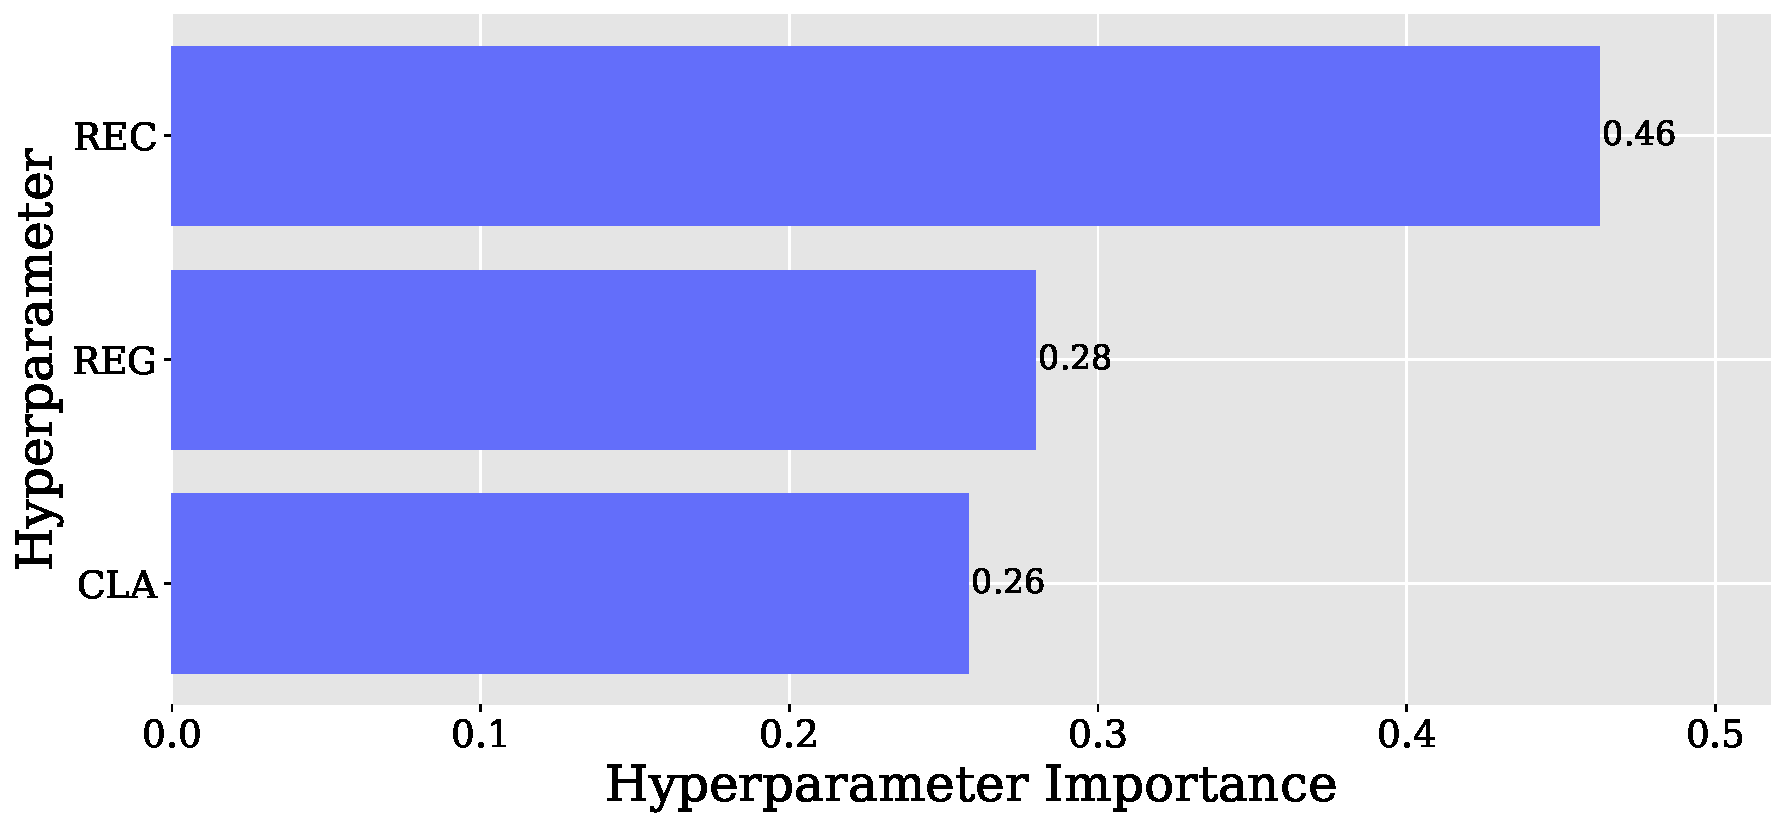
\includegraphics[width=0.8\linewidth]{Figures/optuna_fanova_param_importances_TDHA_NRVAE.pdf}
    \caption{{Global hyperparameter importance of the optimized \gls{eeggcirnet} loss weights on the \gls{adhd}/control children dataset under the SGKF-CV protocol. The importance scores quantify the relative contribution of reconstruction (REC), classification (CLA), and latent-space regularization (REG) weights to validation accuracy.}}
    \label{fig:TDHA_NRVAE}
\end{figure}
%----------------------------------------------------

{The global importance analysis in Figure~\ref{fig:TDHA_NRVAE} shows that REC is the most influential loss-weight hyperparameter in the \gls{adhd}/control children dataset, with an importance score of $0.46$, followed by REG ($0.28$) and CLA ($0.26$). This result indicates that, under strict subject-group validation, validation accuracy is primarily shaped by the model's ability to preserve and reconstruct stable connectivity-based representations. At the same time, the comparable contributions of REG and CLA suggest that latent-space stabilization and discriminative supervision remain necessary to support classification under heterogeneous train--test subject splits. Therefore, \gls{eeggcirnet} does not rely exclusively on the classification objective; instead, it benefits from a multi-objective balance in which reconstruction fidelity plays a central role while regularization and classification provide complementary support. This behavior is consistent with the known difficulty of subject-independent \gls{eeg} generalization under inter-subject variability and heterogeneous neural patterns~\cite{lotte2018review,saha2020intra,lenartowicz2018adhd}.}
%----------------------------------------------------

\subsubsection{Qualitative Analysis of Learned Representations and Functional Connectivity}

The adaptive weighting strategy of the proposed loss function directly influences the quality of the learned representations, which can be assessed by analyzing the decoder's output. Figures~\ref{fig:band14} and~\ref{fig:band27} present the class-specific topographic reconstructions for a representative ``Good'' subject (Subject $14$) and a ``Mid'' subject (Subject $27$). For Subject $14$, the reconstructions are spatially homogeneous, reflecting the ``Good'' group's balanced optimization where the model maintains a stable, regularized latent space. Conversely, for Subject $27$, the reconstructions appear sharper and more structurally defined. This aligns perfectly with the ``Mid'' group's adaptive increase in the reconstruction weight ($\lambda_{\text{REC}}$), which forces the model to prioritize structural fidelity to capture the more complex or noisy signal distributions inherent to this group. The ability to generate coherent and class-consistent topographic maps demonstrates that the VAE successfully captures relevant spatio-spectral patterns.

To validate that these reconstructed topographies represent genuine neural interactions rather than artifacts, we analyzed the underlying functional connectivity networks. Figure~\ref{fig:connectivities} illustrates the average connectivity patterns for the same representative subjects ($14$ and $27$), organized by anatomical region and hemisphere. The edges represent the strongest functional connections ($95$-th to $100$-th percentile), revealing distinct network topologies associated with performance levels.

\begin{figure}[H]
    \centering
    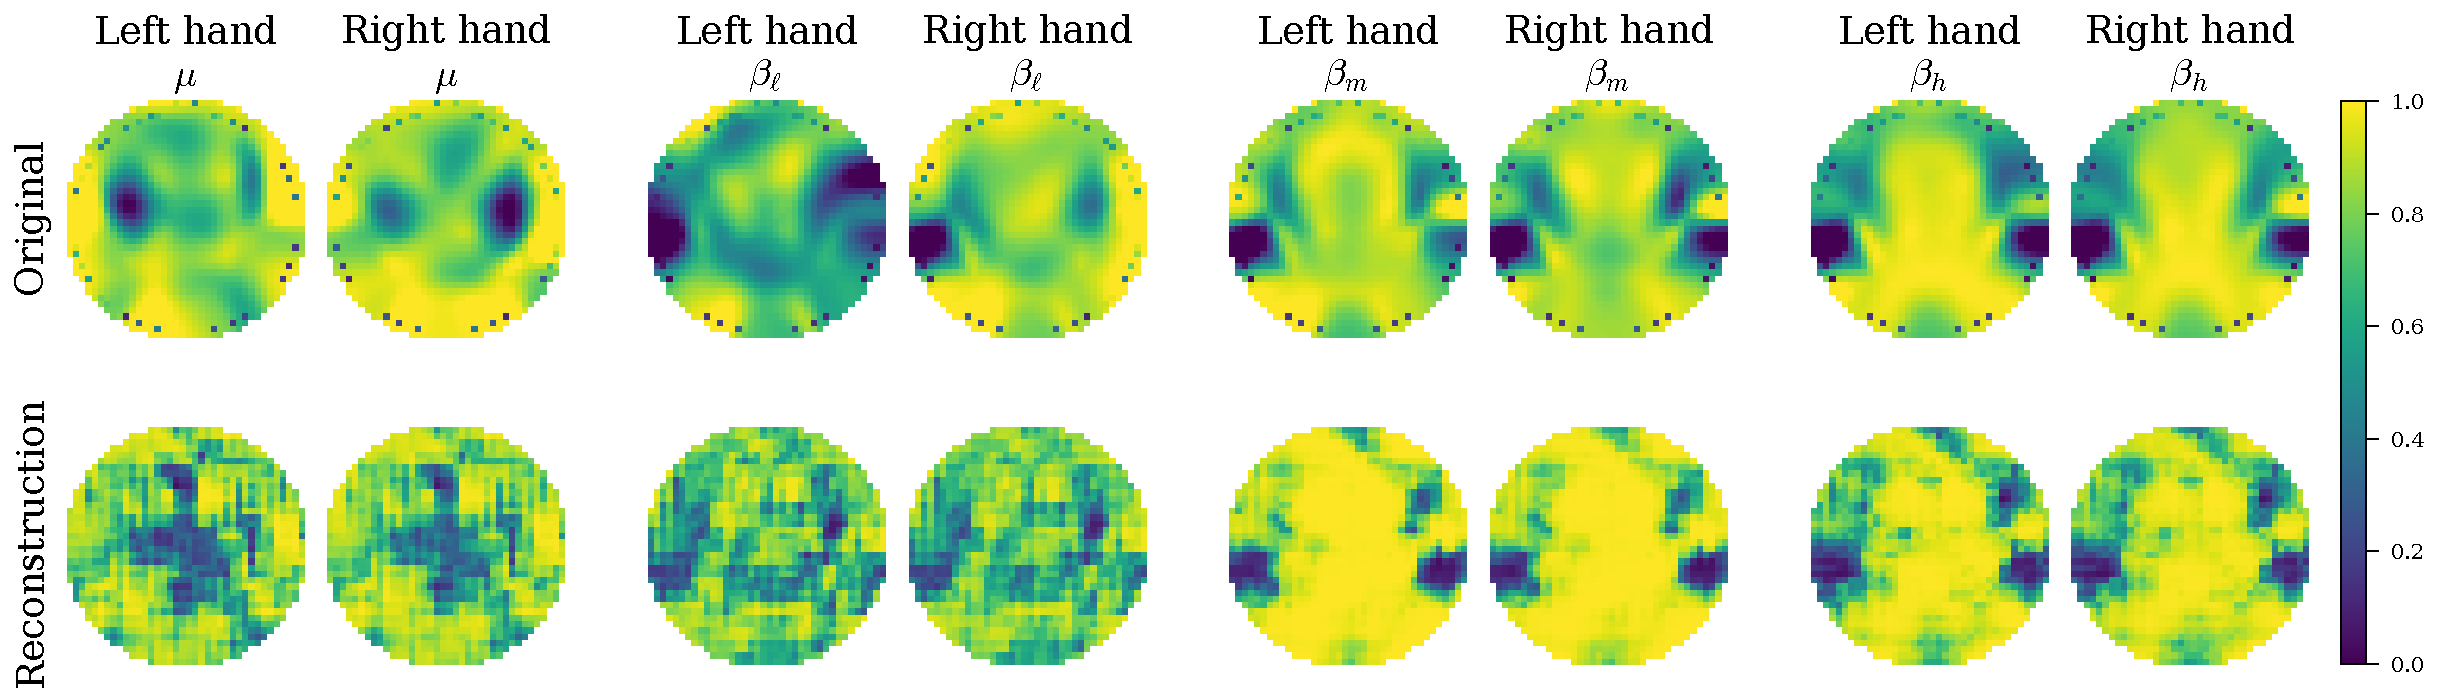
\includegraphics[width=1\linewidth]{Figures/topomaps_bands_14.pdf}
    \caption{Reconstruction subject 14 corresponding to group ``Good''.}
    \label{fig:band14}
\end{figure}
\vspace{-10pt}
\begin{figure}[H]
    \centering
    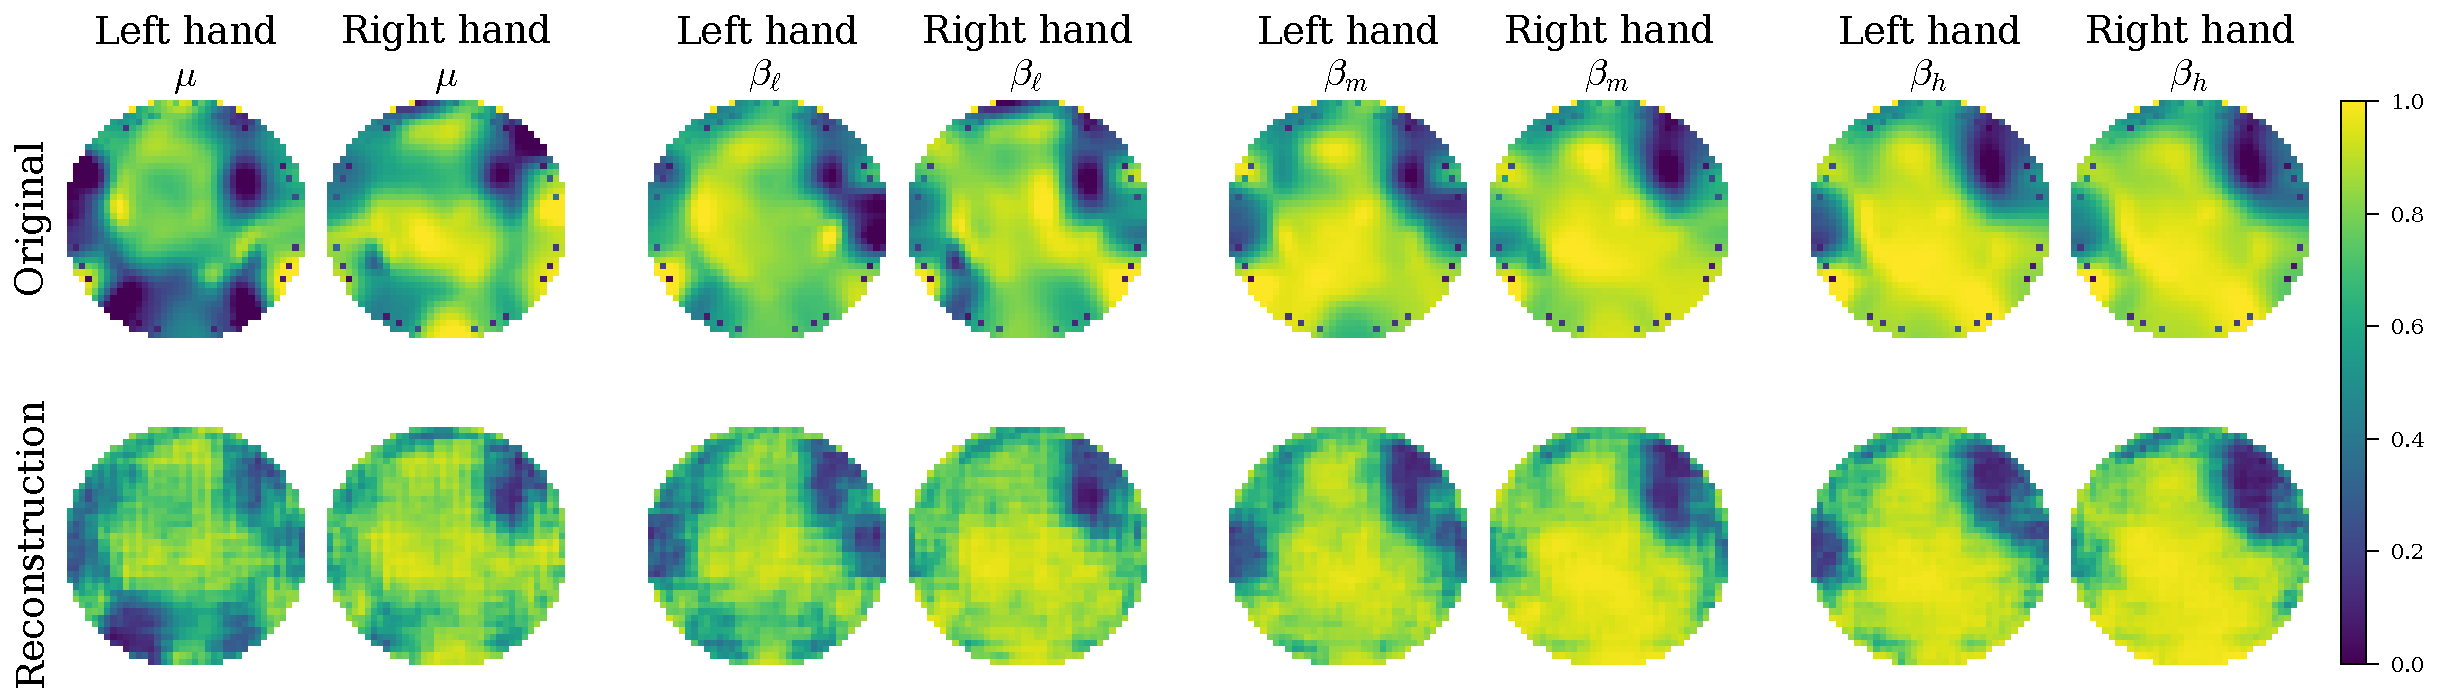
\includegraphics[width=1\linewidth]{Figures/topomaps_bands_27.pdf}
    \caption{Reconstruction subject 27 representing group ``Mid''.}
    \label{fig:band27}
\end{figure}

In the case of the high-performing Subject $14$, the connectivity patterns reveal a highly integrated network. In the $\mu$ band, relevant connections link frontal regions to the right central area, and from there to posterior regions (e.g., P2 to Pz), suggesting a cohesive fronto-centro-parietal network. As the frequency increases into the $\beta$ bands ($\beta_l$, $\beta_m$, $\beta_h$), this integration intensifies. We observe consistent inter-hemispheric links among posterior regions and salient connections bridging midline and left frontal regions (e.g., Fz--F1). This coordinated involvement of bilateral frontal cortices and the sustained posterior coupling supports the notion that high performance is driven by robust long-range synchronization.

In contrast, the connectivity profile of the mid-performing Subject $27$ indicates a different neural strategy, necessitating the model's enhanced focus on reconstruction. Across the $\mu$ and low-$\beta$ bands, connections are heavily concentrated along the central and centro-parietal midline (particularly C1--Cz and CP1--CPz), with a prominent additional link emerging between Pz and P1. Unlike the broad integration seen in the good performer, this subject exhibits a redistribution of connectivity toward fronto-central and centro-posterior networks. In the mid- and high-$\beta$ bands, this configuration remains stable, highlighting a sustained involvement of left posterior parietal regions.
%-----------------------------------------------
\begin{figure}[H]
         \subfloat[Subject 14 group good]{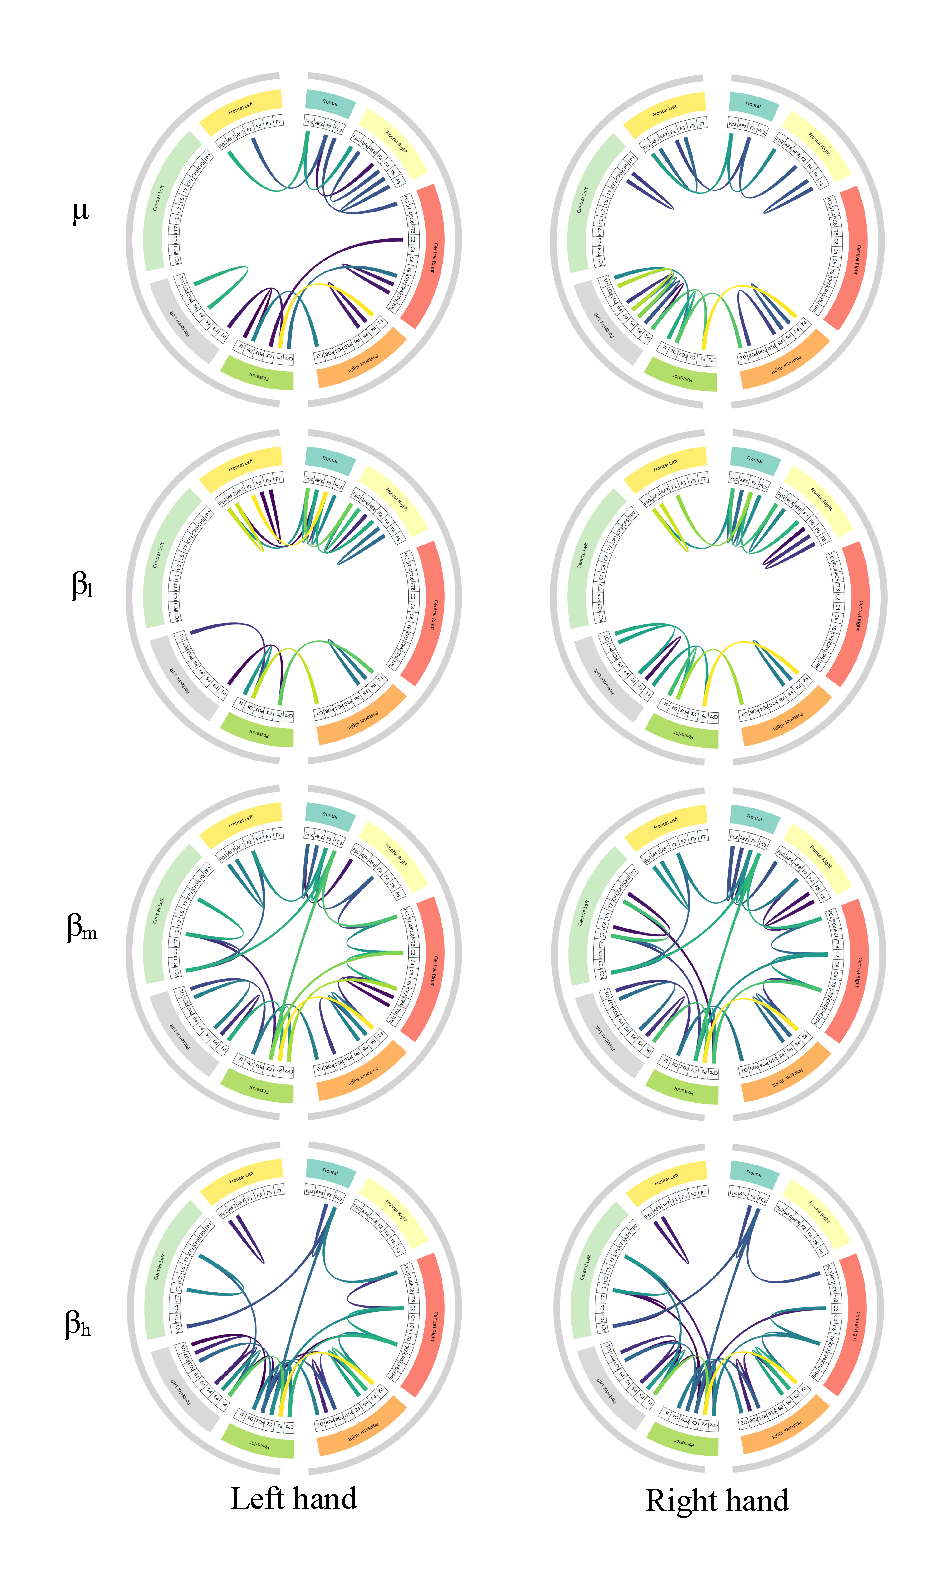
\includegraphics[height=11cm]{Figures/14.pdf}}
         \label{fig:14}
         \subfloat[Subject 27 group mid]{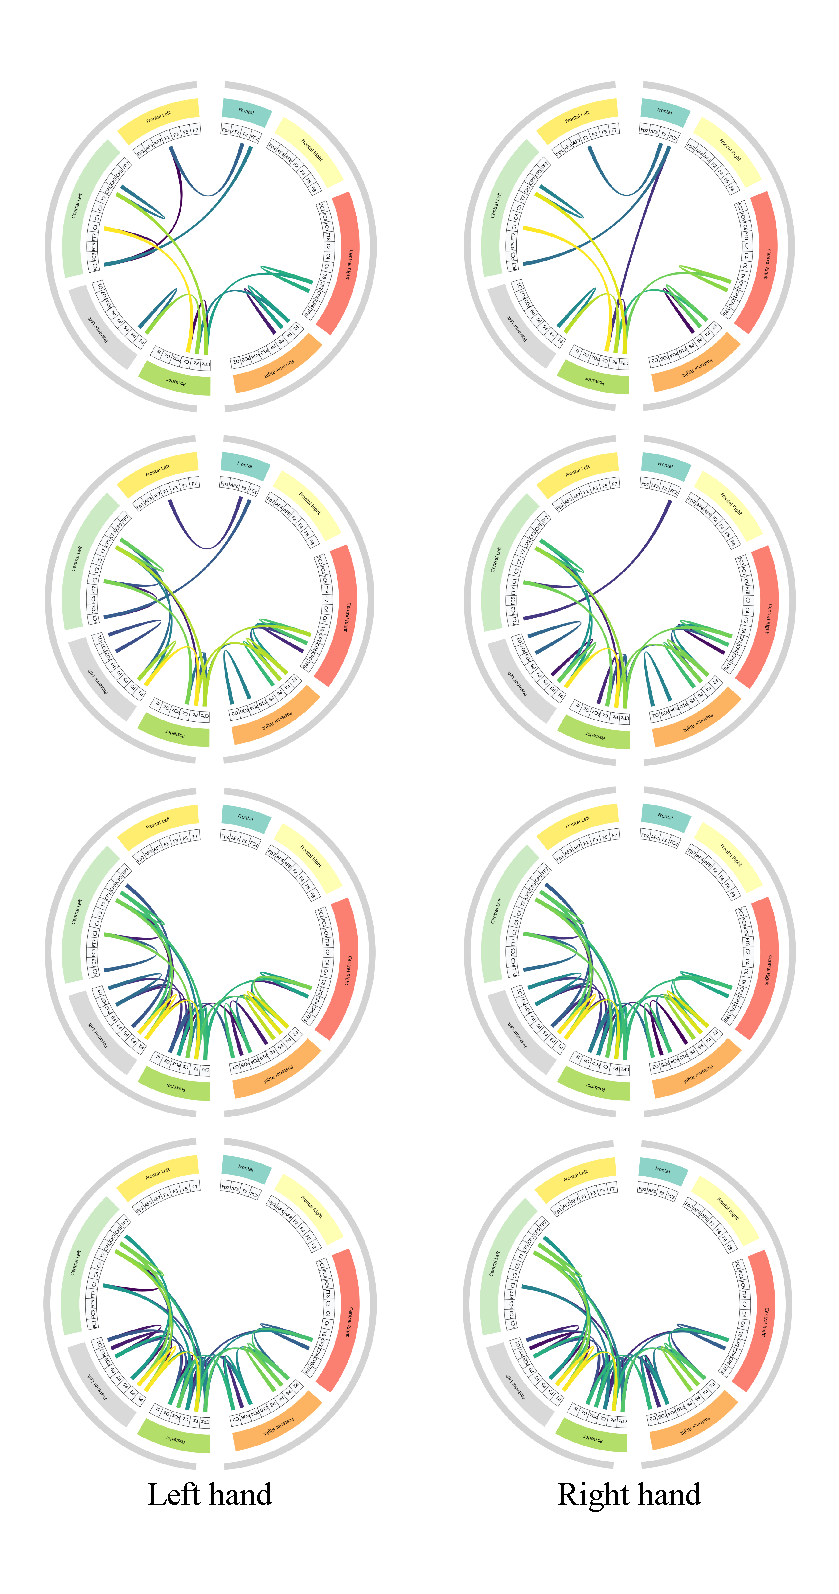
\includegraphics[height=11cm]{Figures/27.pdf}}
         \label{fig:27}
    \vspace{0.4em}
    \begin{tikzpicture}
      \begin{axis}[
        hide axis,
        scale only axis,
        height=0,
        width=0.9\textwidth,
        colormap/viridis,
        colorbar horizontal,
        point meta min=0.86,
        point meta max=1.0,
        colorbar style={
          width=0.9\linewidth,
          height=2mm,
          xlabel={Connectivity},
          xtick={0.86,0.90,0.94,0.98,1.00},
          xticklabel style={font=\small},
        },
      ]
        \addplot [draw=none] coordinates {(0,0) (1,1)};
      \end{axis}
    \end{tikzpicture}

    \caption{Functional connectivity patterns for two representative subjects. For each subject, the left and right columns correspond to left- and right-hand \gls{mi}, respectively, and the rows correspond to the  $\mu$, $\beta_l$, $\beta_m$, and $\beta_h$ bands.}
    \label{fig:connectivities}
\end{figure}
%-----------------------------------------------

The persistence of these specific frequency-dependent connections over sensorimotor and parietal areas in both subjects confirms that the reconstructed maps are biologically valid. The model effectively captures the integrated fronto-parietal networks typical of high performers, as well as the more localized, midline-focused compensatory networks of mid performers. This demonstrates that the \gls{eeggcirnet} does not simply memorize input images, but learns to encode and reconstruct the underlying physiological connectivity drivers of \gls{mi}.

\subsubsection{Structure and Separability of the Latent Space}

The ultimate outcome of the model's adaptive learning and representation quality is a well-structured and discriminative latent space. To visualize this, t-SNE projections were applied to the latent representations of subjects $14$ and $27$ (Figure~\ref{fig:tsne}).

For the high-performing subject $14$ (Figure~\ref{fig:tsne}a), the projection reveals two clearly differentiated and cohesive clusters corresponding to the left- and right-hand MI classes. This well-defined separation confirms that the model has learned a highly discriminative latent space, which is consistent with the subject's high classification accuracy. For the mid-performing subject $27$ (Figure~\ref{fig:tsne}b), the classes are still largely separable, though with some regions of overlap. This is typical for signals with lower quality, where features are partially discriminative but affected by noise~\cite{lee2022intertask, ng2023unsupervised, mishra2024adversarial}.

%------------------------------------------------
\begin{figure}[htbp]
         \subfloat[Subject 14 group good]{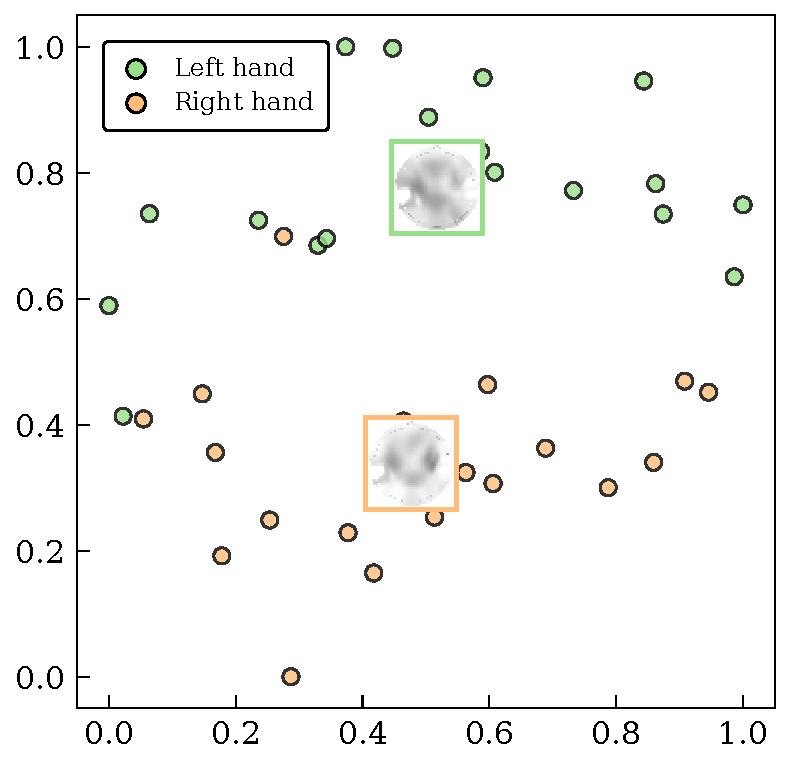
\includegraphics[height=6.5cm]{Figures/t-SNE-14-NRVAE.pdf}}
         \label{fig:tsene14_NRVAE}
     \hfill
     \subfloat[Subject 27 group mid]{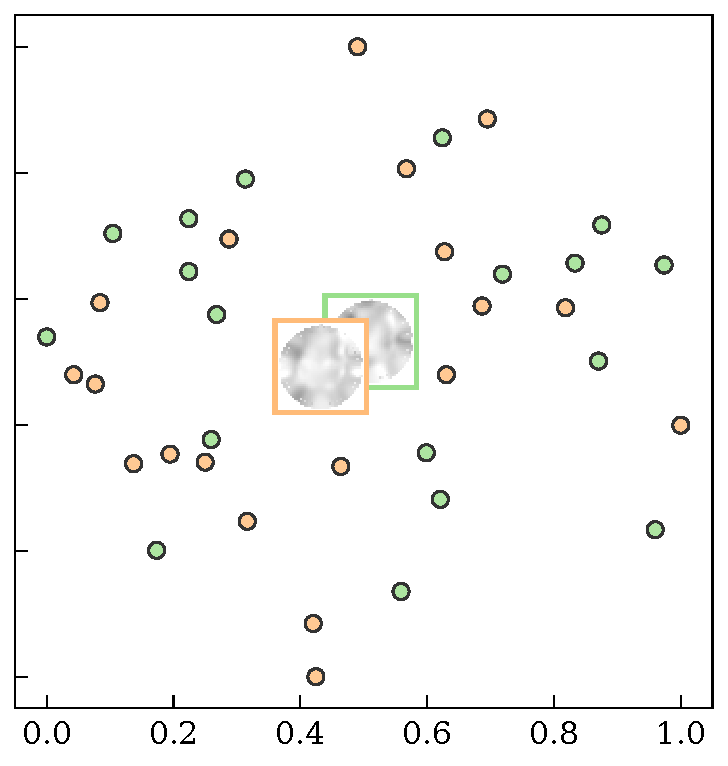
\includegraphics[height=6.5cm]{Figures/t-SNE-27-NRVAE.pdf}}
         \label{fig:tsne27_NRVAE}
    \caption{t-SNE of latent representations by performance group, good and mid. Colors correspond to the \gls{mi} classes (left hand and right hand).}
    \label{fig:tsne}
\end{figure}
%------------------------------------------------

Taken together, these visualizations confirm that \gls{eeggcirnet}'s VAE-based design successfully creates a more structured and discriminative latent space than is typically achievable with standard architectures. This underscores the critical role of latent space regularization in adapting to inter-subject variability and improving generalization, even in the presence of noisy inputs~\cite{ahmed2022latent, sharma2023review}.

\subsubsection{Layer-Wise Relevance Analysis via Grad-CAM++}

{Figure~\ref{fig:cams_subjects} displays the Grad-CAM++ relevance maps in the channel--subject plane for each of the three convolutional layers of the proposed architecture (\texttt{conv1}, \texttt{conv2}, and \texttt{conv3}) and for both MI classes. Unlike aggregate measures, this visualization presents the CAM corresponding to the model trained on that specific subject separately for each layer and class. It is important to note that these maps do not represent static filter weights; rather, they quantify the spatial contribution of each electrode to the model's decision, computed via the gradient-weighted combination of feature maps.}


{In the first convolutional layer (\texttt{conv1}), both classes exhibit broadly distributed activations across subjects and channels, indicating that this layer primarily captures generic spatio-spectral patterns. As the data propagates to \texttt{conv2}, the contribution becomes noticeably more focal, exhibiting clearly delineated channel-wise regions that depend on the MI class. This shift suggests that the model begins to combine spatial and channel information in a more specific manner. Finally, in the deepest layer (\texttt{conv3}), the CAMs become highly sparse and localized, concentrating on a small subset of subjects and channels. This behavior is consistent with a higher degree of specialization, where the deepest layer extracts highly discriminative features directly linked to the final MI decision.}

{Importantly, the CAM amplitudes are not trivially explained by the classification accuracy of each subject. Some subjects with high MI performance still show relatively diffuse or low-amplitude CAMs, whereas others with lower performance may exhibit more pronounced, localized patterns. This indicates that Grad-CAM++ is highlighting how each subject-specific model internally assigns importance to channels to solve the MI task, rather than simply mirroring inter-subject performance differences. Nevertheless, despite training a separate model per subject, the importance maps reveal consistent horizontal bands across subjects, pointing to a degree of cross-subject convergence in the channels that the network considers informative for left- and right-hand MI.}\\


\newlength{\camswidth}
\begin{figure}[H]
  
  \setlength{\camswidth}{0.44\textwidth}% ancho de cada subfigura

  \hspace*{-2em}%
  \makebox[\textwidth]{%
    % ==== Columna izquierda: etiqueta vertical "Channels" ====
    \begin{minipage}[c]{0.18\textwidth}
      \centering
      \rotatebox{90}{\normalsize Channels}
    \end{minipage}%
    \hspace{-1em}% ajusta este espacio si quieres acercar/alejar

    % ==== Columna derecha: las 6 subfiguras + colorbar ====
    \begin{minipage}[c]{0.90\textwidth}
      \centering
      \vspace{4pt}

      % ===== Fila 1 =====
      \subfloat[conv1 -- Left]{%
        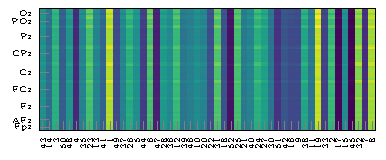
\includegraphics[width=\camswidth]{Figures/Conv1_Left.pdf}%
      }\hspace{0.3em}%
      \subfloat[conv1 -- Right]{%
        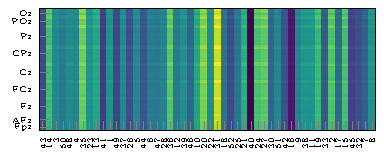
\includegraphics[width=\camswidth]{Figures/Conv1_Right.pdf}%
      }\\[0.5em]

      % ===== Fila 2 =====
      \subfloat[conv2 -- Left]{%
        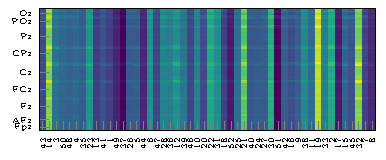
\includegraphics[width=\camswidth]{Figures/Conv2_Left.pdf}%
      }\hspace{0.3em}%
      \subfloat[conv2 -- Right]{%
        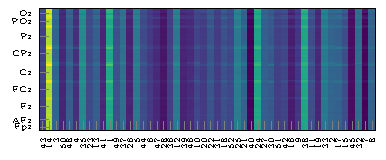
\includegraphics[width=\camswidth]{Figures/Conv2_Right.pdf}%
      }\\[0.5em]

      % ===== Fila 3 =====
      \subfloat[conv3 -- Left]{%
        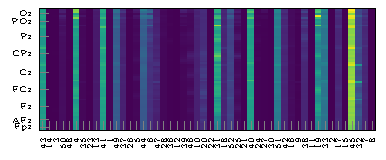
\includegraphics[width=\camswidth]{Figures/Conv3_Left.pdf}%
      }\hspace{0.3em}%
      \subfloat[conv3 -- Right]{%
        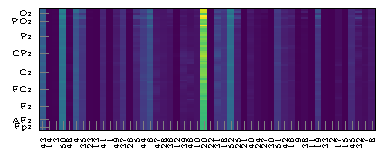
\includegraphics[width=\camswidth]{Figures/Conv3_Right.pdf}%
      }\\[0.8em]

      % ===== Barra de color compartida (creada en TikZ) =====
      \begin{tikzpicture}
        \begin{axis}[
          hide axis,
          scale only axis,
          width=0.9\textwidth,   % largo de la barra
          height=0pt,
          colormap/viridis,
          colorbar,
          colorbar horizontal,
          point meta min=0,
          point meta max=9000, 
          colorbar style={
          width=1\linewidth,
          height=2mm,
          xtick={0,2000,4000,6000,8000},
          xticklabel style={
          font=\scriptsize,
          /pgf/number format/1000 sep={} % ← sin comas en 2,000 → 2000
          },
          xlabel={Channel importance (CAM)},
          xlabel style={font=\scriptsize, yshift=2pt},
          scaled ticks=false,
          /pgf/number format/fixed,
          /pgf/number format/precision=0,
          },
        ]
          % Plot fantasma solo para que pgfplots dibuje la barra
          \addplot[draw=none] coordinates {(0,0)};
        \end{axis}
      \end{tikzpicture}

    \end{minipage}% 
  }
  \caption{Channel-wise CAM contribution across subjects for each convolutional layer and MI class. The color intensity represents the relative importance of each channel in the model's decision-\mbox{making process}.}
  \label{fig:cams_subjects}
\end{figure}

To assess whether the interpretability of the learned features holds in the more complex multi-class scenario, we extended the Grad-CAM++ analysis to the \gls{eegmmidb} dataset. Figure~\ref{fig:cams_subjects1} depicts the relevance maps for four representative classes (C1--C4) across the network depth. Consistent with the binary classification findings, the network exhibits a clear hierarchical refinement of spatial contribution. 


% =========================================================
% =========================================================
% FIGURE: Channel-wise CAMs (solo MI C1--C4, compacta)
% =========================================================
\begin{figure}[H]


% ---------- Dimensiones ----------
\setlength{\camswidth}{0.215\textwidth} % 4 columnas

\newlength{\camsheight}
\setlength{\camsheight}{2.0cm}

\makebox[\textwidth][c]{%

% ================= ETIQUETA VERTICAL =================
\begin{minipage}[c]{0.035\textwidth}
  \centering
  \rotatebox{90}{\normalsize Channels}
\end{minipage}%
\hspace{0.6em}

% ================= MATRIZ 3 × 4 =================
\begin{minipage}[c]{0.94\textwidth}
\centering

% ================= FILA 1 : conv1 =================
\subfloat[conv1--C1]{%
  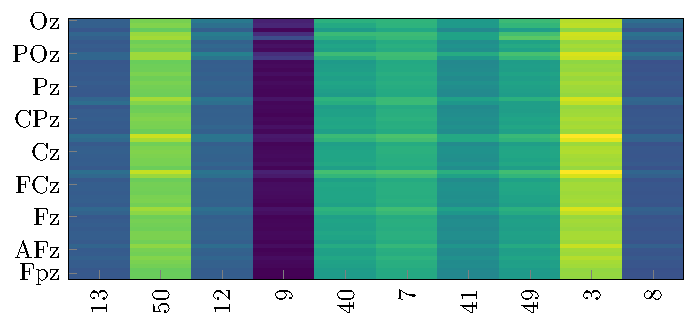
\includegraphics[width=\camswidth,height=\camsheight]{Figures/Conv1 Class1.pdf}} \hfill
\subfloat[conv1--C2]{%
  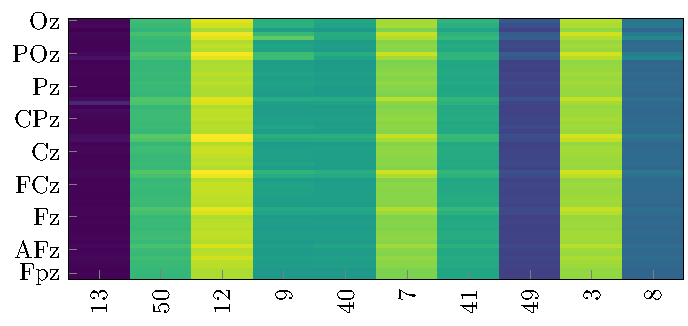
\includegraphics[width=\camswidth,height=\camsheight]{Figures/Conv1 Class2.pdf}} \hfill
\subfloat[conv1--C3]{%
  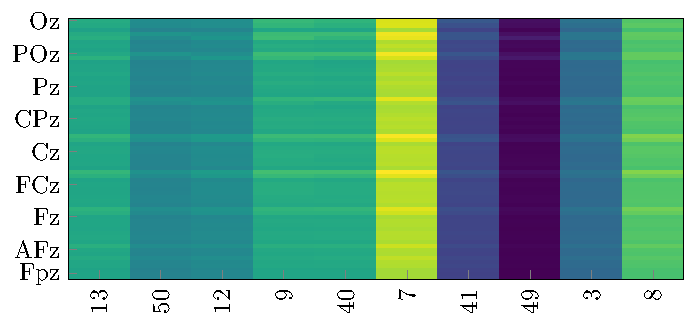
\includegraphics[width=\camswidth,height=\camsheight]{Figures/Conv1 Class3.pdf}} \hfill
\subfloat[conv1--C4]{%
  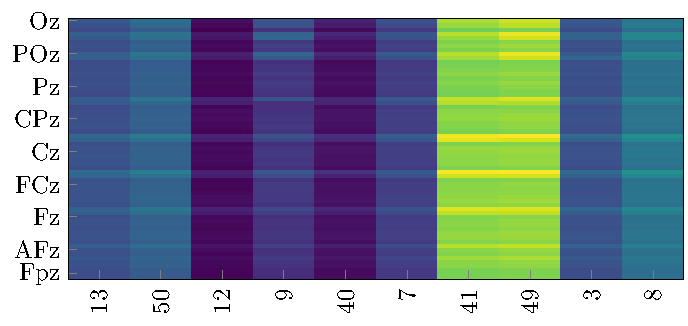
\includegraphics[width=\camswidth,height=\camsheight]{Figures/Conv1 Class4.pdf}} \\[0.3em]

% ================= FILA 2 : conv2 =================
\subfloat[conv2--C1]{%
  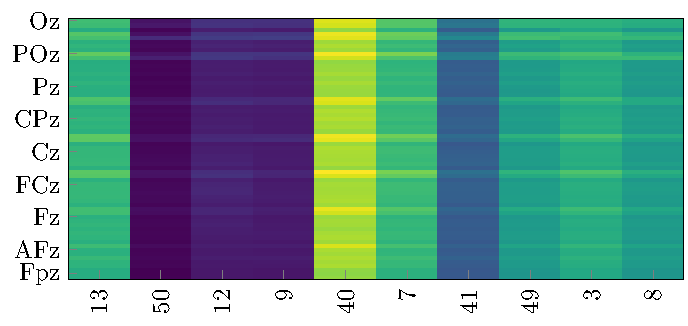
\includegraphics[width=\camswidth,height=\camsheight]{Figures/Conv2 Class1.pdf}} \hfill
\subfloat[conv2--C2]{%
  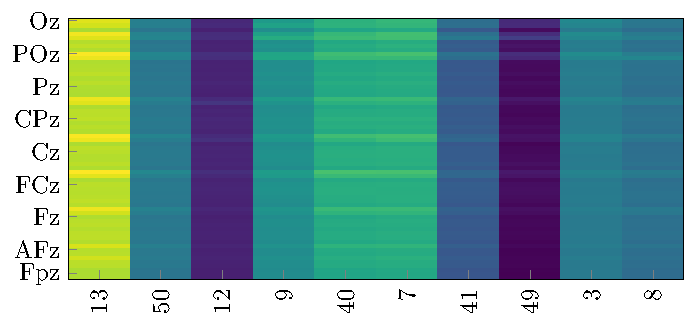
\includegraphics[width=\camswidth,height=\camsheight]{Figures/Conv2 Class2.pdf}} \hfill
\subfloat[conv2--C3]{%
  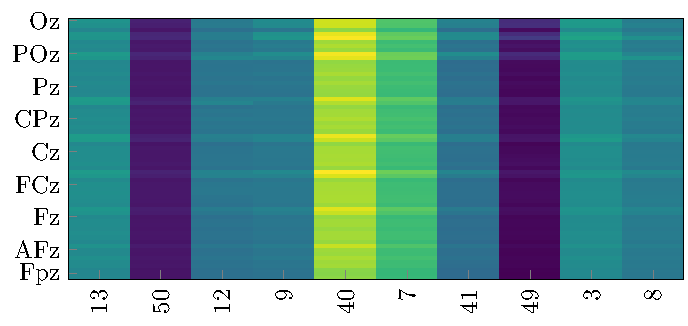
\includegraphics[width=\camswidth,height=\camsheight]{Figures/Conv2 Class3.pdf}} \hfill
\subfloat[conv2--C4]{%
  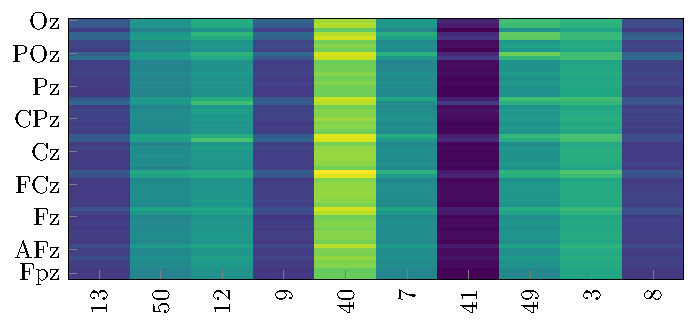
\includegraphics[width=\camswidth,height=\camsheight]{Figures/Conv2 Class4.pdf}} \\[0.3em]

% ================= FILA 3 : conv3 =================
\subfloat[conv3--C1]{%
  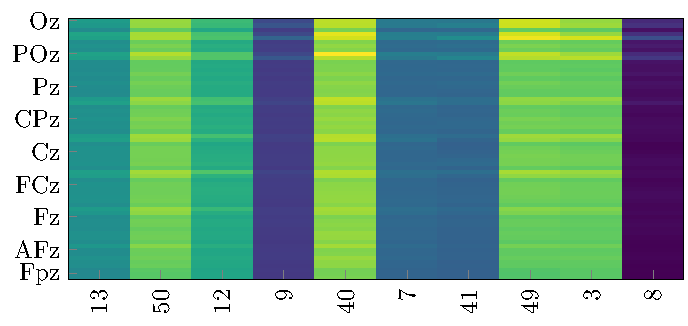
\includegraphics[width=\camswidth,height=\camsheight]{Figures/Conv3 Class1.pdf}} \hfill
\subfloat[conv3--C2]{%
  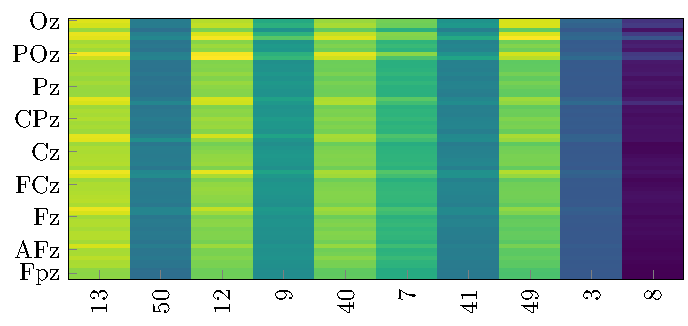
\includegraphics[width=\camswidth,height=\camsheight]{Figures/Conv3 Class2.pdf}} \hfill
\subfloat[conv3--C3]{%
  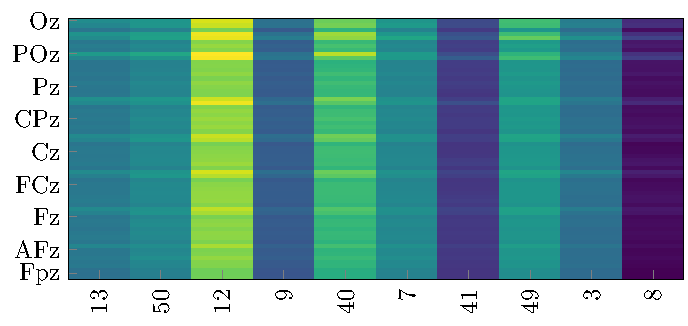
\includegraphics[width=\camswidth,height=\camsheight]{Figures/Conv3 Class3.pdf}} \hfill
\subfloat[conv3--C4]{%
  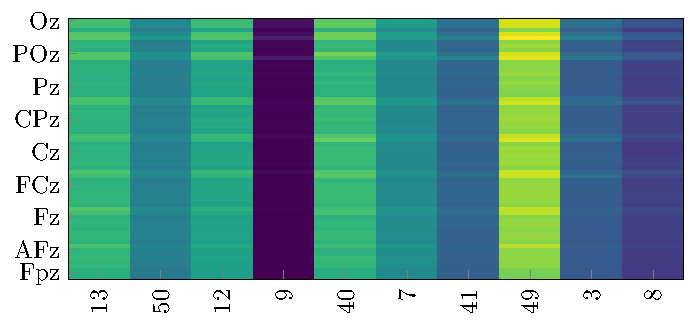
\includegraphics[width=\camswidth,height=\camsheight]{Figures/Conv3 Class4.pdf}} \\[0.7em]

% ================= COLORBAR =================
\hspace{-6pt}\begin{tikzpicture}
\begin{axis}[
  hide axis,
  scale only axis,
  width=0.99\textwidth,
  height=0pt,
  colormap/viridis,
  colorbar,
  colorbar horizontal,
  point meta min=0,
  point meta max=45000,
  colorbar style={
  width=1\linewidth,
  title={Subjects},
  height=2.8mm,
  xtick={0,10000,20000,30000,40000},
  xticklabel style={font=\scriptsize},
  xlabel={Channel importance (CAM)},
  xlabel style={font=\scriptsize, yshift=2pt},
  scaled ticks=false,
  /pgf/number format/fixed,
  /pgf/number format/precision=0,
},
]
\addplot[draw=none] coordinates {(0,0)};
\end{axis}
\end{tikzpicture}

\end{minipage}
}

% ================= CAPTION =================
\caption{Channel-wise class activation maps (CAMs) for \gls{mi} (MI) classes across convolutional layers.
Rows correspond to \textit{conv1}, \textit{conv2}, and \textit{conv3}, while columns (C1--C4) denote the selected MI classes.
Color intensity reflects the relative contribution of each \gls{eeg}channel, using a shared global color scale.}

\label{fig:cams_subjects1}
\end{figure}


In the initial layer (conv1, \mbox{Figure~\ref{fig:cams_subjects1}a--d}), the importance distribution is diffuse and spans vertically across nearly all channels for every class. This suggests that the shallow layers are primarily responsible for extracting low-level, generic spectral features shared among all motor tasks. However, as information flows to the deeper layers (conv3, \mbox{Figure~\ref{fig:cams_subjects1}}i--l), a high degree of spatial \mbox{specialization emerges}.

Notably, the multi-class scenario requires the model to resolve finer topological differences than simple hemispheric lateralization. The maps in the deepest layer (conv3) demonstrate that the model successfully learns distinct spatial signatures for each class. For instance, the channels contributing to Class 1 (Figure~\ref{fig:cams_subjects1}i) form a specific cluster that differs topographically from the channels driving the decision for Class 3 (Figure~\ref{fig:cams_subjects1}k). This spatial disentanglement confirms that \gls{eeggcirnet} solves the complex 5-class problem by isolating specific subsets of task-relevant electrodes—likely corresponding to the distinct cortical representations of hands and feet—rather than relying on global signal artifacts.

%------------------------------------------------
\subsection{Discussion}\label{sec:Discussion1}
%------------------------------------------------

The results obtained with the proposed \gls{eeggcirnet} architecture provide valuable insights into how model design and latent regularization can jointly address key challenges in \gls{mi} decoding. This study demonstrated that by transforming functional connectivity into an image-based representation and processing it with a variational autoencoder, it is possible to create a BCI framework that is not only highly accurate but also robust and interpretable. The model achieved remarkable performance across subjects, reaching the highest average accuracy ($81.82\%$) and the lowest inter-subject variability among all evaluated methods, confirming the efficacy of this unimodal, VAE-based approach.

{A key aspect of this contribution} lies in its direct response to the critical challenges of inter-subject variability and ``BCI illiteracy''. The most compelling finding was the complete elimination of the ``Bad'' performance group (Figure~\ref{fig:Violins}c), coupled with substantial accuracy gains of $21.55\%$ and $13.70\%$ for the ``Bad'' and ``Mid'' groups, respectively (Table~\ref{tab:accuracy_gain}). This demonstrates the profound robustness of \gls{eeggcirnet} in handling noisy or low-separability \gls{eeg} signals, where conventional architectures typically fail. By elevating the performance of these challenging subjects, the framework serves a corrective function, suggesting a promising path toward more inclusive and reliable BCI systems that can adapt to a wider range of users. {Furthermore, the scalability of the proposed framework is evidenced by its superior performance in the complex 5-class \gls{eegmmidb} scenario, where it achieved an average accuracy of $75.20\%$, surpassing advanced temporal-channel fusion models by approximately $6.3$\%. Unlike binary tasks, where hemispheric lateralization is often sufficient for discrimination, the 5-class problem requires the model to resolve finer topological differences between spatially overlapping classes, such as ``Both Hands'' versus single-hand imagery.

The mechanism underlying this robustness appears to be the model's sophisticated, adaptive learning strategy. The analysis of the loss weight distributions (Figure~\ref{fig:distributions}) revealed that \gls{eeggcirnet} is not a static ``black box'' but dynamically reorganizes its optimization priorities based on signal quality. In the bi-class scenario, for subjects with high-quality signals, it maintains a harmonious balance between reconstruction, classification, and regularization. For subjects with more challenging signals, it strategically prioritizes representation learning (REC loss) over immediate classification (CLA loss). This intelligent trade-off is visually confirmed by the qualitative analysis of the reconstructions (Figures~\ref{fig:band14} and~\ref{fig:band27}), which shows that the model consistently generates spatially coherent and physiologically plausible connectivity maps. This behavior supports the notion that a well-regularized and accurately reconstructed representation is a prerequisite for effective classification, especially in noisy conditions. {Moreover, as observed in Table~\ref{tab:weights_dist}, for the most challenging subjects (e.g., Subject 49) in multi-class scenario, the network implicitly shifts its role from a classifier to a non-linear denoiser ($\lambda_{\text{REC}} \approx 0.83$), prioritizing the reconstruction of a clean latent representation before attempting to separate complex decision boundaries. This suggests that the connectivity-driven topographic maps provide a sufficiently rich feature space to support multi-class decoding, provided that the training objective is dynamically regularized to handle the increased cognitive load and signal ambiguity.

The above is further corroborated by the functional connectivity analysis, which reveals distinct network topologies associated with performance levels (see Figure~\ref{fig:connectivities}). For high-performing subjects, the observed integrated fronto--centro--parietal network supports established findings on the critical role of fronto--parietal and parieto--occipital connectivity in supporting MI performance~\cite{Hamedi2016MIBrainConnectivityReview}, while the specific beta-band synchronization over central and parietal regions aligns with literature identifying these features as informative markers for task discrimination~\cite{cardoso2021pedalingMI}. Conversely, the connectivity profile of mid-performing subjects suggests a redistribution toward fronto--central and centro--posterior networks; notably, the persistence of $\mu/\beta$-band connections over sensorimotor and parietal areas in these subjects remains consistent with studies highlighting the fundamental role of these networks in effective BCI control~\cite{CaicedoAcosta2021DeepNeuralRegression,Vidaurre2020SensorimotorFC}.

The ultimate outcome of this adaptive process is the creation of a well-structured and discriminative latent space. The t-SNE visualizations (Figure~\ref{fig:tsne}) provide direct evidence that the encoder successfully learns to disentangle the features of different MI classes, creating clearly separated clusters for high-performing subjects and maintaining reasonable separation even for mid-performing subjects. This demonstrates that the variational formulation and structured latent regularization are the primary drivers of the model's superior performance, allowing it to move beyond the limitations of conventional architectures that often struggle with noisy or overlapping feature distributions.

To verify that these learned latent structures correspond to genuine neural mechanisms rather than artifacts, we examined the spatial contribution patterns identified by the network. The layer-wise analysis of the relevance maps reveals consistent spatial structures that align with anatomically meaningful channel groups (see Figure~\ref{fig:cams_subjects} and~\ref{fig:cams_subjects1}). High-contribution areas in the superior frontal region likely reflect higher-order cognitive control and attentional processes facilitating MI, consistent with reports of prefrontal involvement linked to imagery quality ~\cite{hetu2013neural,delange2008cortex,kurkin2023tmsdlpfc}. Meanwhile, prominent bands of importance spanning fronto-central and parietal sites correspond to the well-known fronto-parietal MI network—encompassing premotor and parietal regions recruited during kinesthetic and visual MI ~\cite{mustile2024walking} and align with established evidence of alpha and beta modulation and information flow across these regions~\cite{zhou2025vmi}. Thus, the specific emphasis on parieto-occipital electrodes in the deepest layers suggests the network leverages visuo-spatial components alongside sensorimotor rhythms, a view supported by studies indicating occipital recruitment and connectivity during visual-\gls{mi}~\cite{dijkstra2024evc}. Regarding the multi-class scenario, the extended Grad-CAM++ analysis confirms that \gls{eeggcirnet} addresses this complexity through hierarchical spatial refinement, evolving from generic spectral features in shallow layers to highly specialized, class-specific electrode clusters in deep layers. This capability is underpinned by the model's adaptive optimization strategy, which becomes even more pronounced in this high-complexity setting. Overall, these results confirm that the proposed architecture converges towards neurophysiologically plausible channel patterns, emphasizing networks repeatedly implicated in motor simulation.

Finally, the statistical analysis confirms the performance advantage of \gls{eeggcirnet} across different levels of task complexity. While the model secured a leading average ranking of $2.32$ ($p=0.007$) in the binary scenario (Table~\ref{tab:p-values_updated}), its dominance became even more pronounced in the multi-class evaluation (Table \ref{tab:p-values_updated1}). In this challenging 5-class setting, \gls{eeggcirnet} achieved a perfect average ranking of ${1.00}$ and a highly significant average Wilcoxon $p$-value of ${0.002}$, establishing a statistically clear superiority over advanced architectures like TCFusionNet and DeepConvNet. This indicates that the observed performance gains are not random fluctuations but a consistent outcome of the model’s design. By learning robust latent structures directly from connectivity-based topographic representations, \gls{eeggcirnet} emerges as a reliable, interpretable, and computationally efficient framework for \gls{mi} decoding. It effectively balances accuracy, generalization, and representational stability, allowing it to adapt to diverse subject profiles and maintain strong performance across varying signal quality conditions while preserving a physiologically consistent representational organization.

%------------------------------------------------
\subsection{Summary}\label{sec:Conclusions1}
%------------------------------------------------
In this chapter, we proposed \gls{eeggcirnet}, a novel unimodal framework based on a variational autoencoder, designed to process topographic representations of functional connectivity for \gls{mi} classification. Through an extensive experimental evaluation, we demonstrated that this approach effectively addresses several persistent challenges in \gls{eeg}-based \glspl{bci}, including low spatial resolution, susceptibility to noise, and inter-subject variability. By integrating Gaussian functional connectivity with a generative VAE architecture, the proposed framework produces spatially structured representations that enable simultaneous classification and reconstruction, providing both competitive performance and interpretability grounded in neurophysiology.

{Overall, the proposed framework demonstrates that} connectivity-driven representations can substantially enhance robustness and subject-level fairness in \gls{mi} decoding. On the binary GigaScience benchmark, \gls{eeggcirnet} achieved the highest average accuracy ($81.82\%$) and the lowest inter-subject variability ($\pm10.15$) among all evaluated baselines. Most notably, the model completely eliminated the ``Bad'' performance group (subjects with $<60\%$ accuracy) and yielded performance gains of approximately $22\%$ for these challenging users. This result, which is statistically significant ($p=0.007$), indicates that the variational formulation enables the extraction of discriminative information even from noisy or low-separability signals. Moreover, in the more complex 5-class \gls{eegmmidb} scenario, \gls{eeggcirnet} achieved a perfect average ranking of ${1.00}$ and a highly significant Wilcoxon $p$-value of ${0.002}$, confirming its scalability to multi-class decoding with overlapping spatial patterns.

Importantly, the generalization capability of the proposed framework was further validated on the BCI Competition IV-2a dataset, a widely standardized and subject-independent benchmark. Subject-wise analyses revealed that \gls{eeggcirnet} consistently outperformed EEGNet across all subjects, with the largest performance gains observed for individuals exhibiting lower baseline accuracies. This behavior highlights the robustness of the connectivity-driven representation to inter-subject variability and demonstrates that physiologically informed feature construction can rival the performance of substantially heavier architectures without increasing model complexity.

The strong empirical performance of \gls{eeggcirnet} is supported by its adaptive optimization behavior. Analysis of the loss component weights revealed that the model dynamically reorganizes its learning priorities based on signal quality. For high-performing subjects, reconstruction, classification, and regularization losses remain balanced, whereas for weaker subjects or high-complexity tasks, the model prioritizes representation learning. This adaptive trade-off allows \gls{eeggcirnet} to function as a non-linear denoiser, resulting in a well-structured latent space where \gls{mi} classes are clearly disentangled, as evidenced by t-\mbox{SNE} visualizations.

Complementary interpretability analyses further confirmed the physiological relevance of the learned representations. Grad-CAM++ visualizations revealed a hierarchical learning process, progressing from generic spectral features in early layers to highly localized, task-relevant activations in sensorimotor and parieto-occipital regions. Functional connectivity analyses demonstrated that the model captures biologically meaningful networks, including long-range fronto--centro--parietal integration in high-performing subjects and compensatory, localized connectivity patterns in mid-performing individuals. These findings confirm that \gls{eeggcirnet} bases its decisions on genuine neurophysiological mechanisms rather than spurious correlations.

Despite these strengths, the limitations of the proposed framework become evident under clinically challenging generalization settings. When evaluated on the \gls{adhd}/control children dataset using a strict Subject-Group K-Fold Cross-Validation protocol, \gls{eeggcirnet} achieved stable but comparatively lower accuracy than several specialized baselines. This result highlights that, in pediatric clinical datasets, the dominant challenge shifts from class separability toward robust subject-to-subject transfer under pronounced neurophysiological heterogeneity. While \gls{eeggcirnet} exhibited consistent behavior across folds, the observed performance gap indicates that connectivity-driven representations alone may be insufficient to fully compensate for domain shifts arising from developmental variability, recording conditions, and individual neurocognitive profiles.

Overall, these findings delineate the operational scope of \gls{eeggcirnet}. The proposed framework is particularly effective for \gls{mi}-based \glspl{bci} and standardized decoding scenarios, where physiologically grounded connectivity representations can substantially reduce inter-subject disparities. However, its performance on the \gls{adhd}/control dataset underscores the need for additional mechanisms—such as domain adaptation, adaptive normalization, or hybrid architectures—to address the extreme variability encountered in clinical pediatric populations. These results provide both validation of the framework’s strengths and clear direction for future extensions aimed at improving subject-independent generalization in real-world clinical \gls{eeg} applications.

%\chapter{\Objectivetwoname}
\chapter[Takens-based Kernel \gls{te} Connectivity Network for \gls{mi} Classification]{Takens-based Kernel \gls{te} Connectivity Network for
\gls{mi} Classification}\label{chapter_2} 
\chaptermark{TEKTE-Net}


\noindent\noindent{\textbf{Interpretative note on causal terminology.}
This chapter is based on a peer-reviewed article previously published by the author 
and included here as part of a unified doctoral research framework. Therefore, the 
methodological terminology of the original publication is preserved. However, in light 
of the discussion presented in Section~\ref{sec:causality_eeg}, the terms 
\emph{causal}, \emph{causal influence}, \emph{causal dependencies}, 
\emph{inter-channel causality}, and related expressions used in this chapter should 
be interpreted in the predictive Wiener--Granger sense commonly adopted in 
neuroscience. Accordingly, \gls{te}-based connectivity is understood here as directed 
information flow or directed predictive dependency at the signal level, rather than as 
definitive evidence of strict interventional, counterfactual, or mechanistic causality.}

%introduccion de 2 parrafos 
Building upon the foundations established by the Gaussian Connectivity-Driven \gls{eeg} Imaging framework, which focused on enhancing functional representation and spatial interpretability, the next step in this research addresses the modeling of effective brain connectivity. While functional connectivity captures statistical dependencies between neural regions, it does not account for the directionality or causal influence of information flow within the brain. Such directional and dynamic interactions are critical for understanding the neural mechanisms underlying motor control and cognitive processing, particularly in \gls{mi} paradigms. Consequently, there is a growing need for computational models that can infer nonlinear and time-dependent relationships directly from \gls{eeg} data, while maintaining interpretability and robustness.

To meet this challenge, {this contribution} introduces the Takens-Based Enhanced Kernel \gls{te}  Network (\gls{tektenet}), a novel deep learning framework designed to estimate and learn directed and nonlinear interactions in \gls{eeg} signals. \gls{tektenet} combines Takens' state-space reconstruction with kernel-based \gls{te}  estimation, allowing the network to represent causal dependencies within a latent connectivity space. By embedding this information into a deep generative model, the framework captures both the temporal dynamics and directional flow of neural activity, bridging the gap between effective connectivity analysis and end-to-end \gls{eeg} decoding. This contribution represents a crucial step toward the development of adaptive, interpretable, and causally informed \gls{bci} systems.

{It is important to clarify that \gls{tektenet} is not intended to replace classical event-related potential (ERP) analysis, nor should it be interpreted as a deeper version of ERP-based evaluation. ERP analysis mainly characterizes time-locked cortical responses in terms of amplitude, latency, and waveform morphology~\cite{Picton2000ERP}. In contrast, \gls{tektenet} aims to provide complementary network-level information by estimating nonlinear, directed, and time-delayed interactions between \gls{eeg} channels. Therefore, while ERP analysis can indicate when a cognitive or sensorimotor response occurs, \gls{tektenet} seeks to characterize how information flows across reconstructed \gls{eeg} state spaces during task-related brain dynamics.}


Figure~\ref{fig:tekte_pipeline} provides a schematic overview of the proposed framework, illustrating the main processing stages from raw \gls{eeg} signals to the estimation of directed connectivity patterns for \gls{mi} classification.

\begin{figure}[htbp]
  \centering
  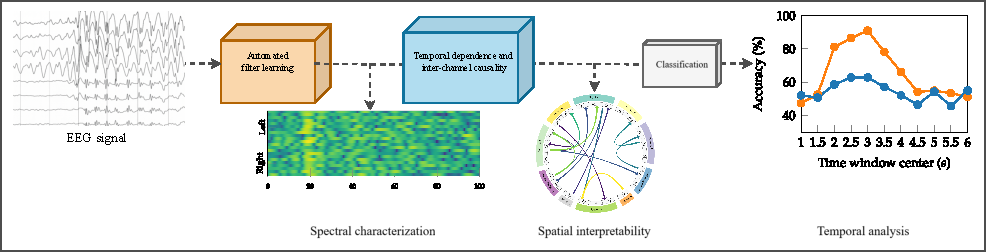
\includegraphics[width=\textwidth]{Figures/Metodology.pdf}
  \caption{Schematic overview of the proposed connectivity-driven framework for \gls{mi} classification. 
  Raw \gls{eeg} signals are processed through automated filter learning and temporal modeling to capture nonlinear and directed inter-channel interactions. 
  The resulting representations enable spectral characterization, spatial interpretability through connectivity patterns, and temporal analysis of task-related dynamics.}
  \label{fig:tekte_pipeline}
\end{figure}

\subsection{Mathematical Framework}\label{sec:Mathematical_Framework}

{This contribution} introduces \gls{tektenet}, a novel end-to-end deep learning architecture designed to model nonlinear spatiotemporal dynamics and directed causal interactions directly from raw \gls{eeg}signals. The model incorporates a customized convolutional module that performs Takens' embedding, enabling the reconstruction of the underlying dynamical system without requiring explicit preprocessing. This mechanism facilitates the extraction of subject-specific, task-relevant temporal and spectral features. A central contribution of \gls{tektenet} is the integration of a fully differentiable \gls{te} estimator, formulated via Rényi's $\alpha$-order entropy and positive-definite kernels, allowing for the estimation of nonlinear, directed information flow between \gls{eeg}channels within a trainable framework. The following sections describe the dataset and mathematical foundations in detail.

\subsubsection{Channel-wise nonlinear time series embedding from Takens' convolutional layer}\label{sec:takens}

Let $\mat{X} \in \mathbb{R}^{T \times C}$ be a discrete multichannel input signal of temporal length $T$ and $C$ channels. The channel-wise nonlinear filtering of the $c$-th channel is denoted as $\ve{\phi}_c=\varphi(\ve{x}_c|\theta_c)$, being $\ve{x}_c\in\Real^T$ its corresponding input time series, $\ve{\phi}_c\in\Real^{T_{\phi}}$ the filtered output of length $T_{\phi}\leq T$. A deep learning strategy nonlinearly filters each channel using $L$ sequential layers parameterized by $\theta_c$, that is, $\varphi(\cdot|\theta_c)=\varphi_{L}(\cdots(\varphi_1(\cdot))$. The usual layers considered in the nonlinear filtering are convolutions, poolings, and dropouts that support extracting complex channel-wise temporal structures and nonlinear dependencies to learn more informative and discriminative representations.

Aiming to take advantage of the \gls{eeg}latent dynamics through the Markovian property, a delay-coordinate Takens' embedding reconstructs the channel-wise state space by stacking time-delayed versions of the nonlinearly-filtered channel $\ve{\phi}_c$ into fixed-length vectors, resulting in a delay-embedded representation $\mat{Z}_{c\mu} \in \mathbb{R}^{T_z \times D}$, where $D \in \mathbb{N}$ denotes the embedding order (i.e., number of delay coordinates), the delay offset $\mu \in \mathbb{N}$, and $T_z\leq T_\phi$. A set of fixed, non-trainable convolutional filters implements the embedding replicating delayed copies of the input without altering the learned parameters as 
\begin{equation}\label{eq:z_takens}
\mat{Z}_{c\mu}=\mat{W}_{D,\tau,\mu}^\top*\ve{\phi}_c
\end{equation}
{where the convolution kernel $\mat{W}_{D,\tau,\mu}\in\{0,1\}^{R \times D}$, with $R = \mu + \tau \cdot (D - 1) + 1$,} depends on three predefined hyperparameters, namely, the delay stride $\tau \in \mathbb{N}$, the embedding order $D$, and the delay offset $\mu$. Such Takens' convolution kernel elements holds elements 
$w_{r,d}=\delta(r - \mu - \tau \cdot d)\forall d \in [0, D-1], r \in [0, {R}-1]$, with $\delta(\cdot)$ as the discrete delta Dirac function. Thus, the full Takens-embedded nonlinearly-filtered signal $\mat{Z}_{c\mu}$ enables the subsequent processing layers to access the temporal structure and to capture directed inter-channel interactions through the reconstructed dynamical states rather than raw observations.

\subsubsection{\gls{te}  from kernel matrices}

{This contribution} assesses the inter-channel interactions through the \gls{te}  which has been proposed as an effective tool for distinguishing between driving and responding elements, as well as for detecting asymmetries in subsystem interactions~\cite{staniek2008symbolic}. Originally introduced by Schreiber~\cite{schreiber2000measuring} and related to the concept of Granger causality~\cite{Sethgranger}, TE operates under the premise that the $c$-th channel $\ve{x}_{c}$ can be considered to causally influence $c'$-th channel $\ve{x}_{c'}$ if incorporating the past of the channel $c$, together with the past of channel $c'$, better predicts the present of $\ve{x}_{c'}$ than using $\ve{x}_{c'}$ past alone, for all discrete time instants $t\in[1,T]$. According to \Cref{sec:takens}, the present of the responding channel $c'$ can be computed from the Takens' delayed-embedding by setting $\mu=0$ and $D=1$, while its past by setting $\mu=1$ and $D=D'$ to be tuned, respectively. In turn, the past of the driving channel $c$ accounts for $D$ time-delayed interactions, thanks to $\mu$, as in \Cref{eq:xt-u}.
\begin{align}
\ve{z}_{c'0}=&\mat{W}_{\tau,1,0}^\top*\ve{\phi}_{c'}\in\Real^{T_z}\label{eq:yt}\\
\mat{Z}_{c'1}=&\mat{W}_{\tau,D',1}^\top*\ve{\phi}_{c'}\in\Real^{T_z\times D'}\label{eq:yt-1}\\
\mat{Z}_{c\mu}=&\mat{W}_{\tau,D,\mu}^\top*\ve{\phi}_c\in\Real^{T_z\times D}\label{eq:xt-u}
\end{align}

Note that the $t$-th row of the Takens' embeddings in \Cref{eq:yt,eq:yt-1,eq:xt-u} correspond to the current state of the responding channel $z_{c't}\in\Real$, the past state of the responding channel $\ve{z}_{c't-1}\in\Real^D$, and the past of the driving channel $\ve{z}_{ct-\mu}\in\Real^D$, respectively, aligned at every time instant $t\in[1,T_z]$. Using those three time-aligned embeddings, \Cref{eq:te_01} formally defines the \gls{te}  $TE(c \to c')$ as the expected information gain about the current state of the responding channel given its own past, i.e., $p\left(z_{c't} \mid \ve{z}_{c't-1}\right)$, when the past of the driving channel is also known, i.e.,  $p\left(z_{c't} \mid \ve{z}_{c't-1},\,\ve{z}_{ct-\mu}\right)$. 
\begin{equation}
    TE(c \to c') = 
    \iiint 
    p\bigl(z_{c't},\,\ve{z}_{c't-1},\,\ve{z}_{ct-\mu}\bigr)\, 
    \log\!\biggl(
      \frac{ 
        p\bigl({z}_{c'} \mid \ve{z}_{c't-1},\,\ve{z}_{ct-\mu}\bigr)
      }{
        p\bigl({z}_{c'} \mid \ve{z}_{c't-1}\bigr)
      }
    \biggr)
    \,d{z}_{c'}\,d\ve{z}_{c't-1}\,d\ve{z}_{ct-\mu}.
\label{eq:te_01}
\end{equation}
Equivalently, it can be written in expectation form as:
\begin{equation}
    TE(c \to c') \;=\; 
\mathbb{E}_{z_{c't},\,\ve{z}_{c't-1},\,\ve{z}_{ct-\mu}}
\Biggl\{
  \log\!\biggl(
    \frac{ 
      p\bigl(z_{c't} \mid \ve{z}_{c't-1},\,\ve{z}_{ct-\mu}\bigr)
    }{
      p\bigl(z_{c't} \mid \ve{z}_{c't-1}\bigr)
    }
  \biggr)
\Biggr\},
\end{equation}
where the expectation operator is defined as 
\begin{equation}
    \mathbb{E}_{z}\{f(z)\} \;=\; \int p(z)\,f(z)\,dz.
\end{equation}

Thanks to Bayes’ rule and logarithm properties, the conditional probabilities in Equation~\eqref{eq:te_01} are split into four terms depending on the joint and marginals as follows:
\begin{align}
 TE(c \to c') &= \mathbb{E}_{z_{c't},\ve{z}_{c't-1},\ve{z}_{ct-\mu}}
      \bigl\{\log p\bigl(z_{c't},\ve{z}_{c't-1},\ve{z}_{ct-\mu}\bigr)\bigr\} \label{eq:TE_expansion1}\\
      &-\mathbb{E}_{z_{c't},\ve{z}_{c't-1},\ve{z}_{ct-\mu}}
      \bigl\{\log p\bigl(\ve{z}_{c't-1},\ve{z}_{ct-\mu}\bigr)\bigr\}\nonumber\\
      &+\mathbb{E}_{z_{c't},\ve{z}_{c't-1},\ve{z}_{ct-\mu}}
      \bigl\{\log p\bigl(\ve{z}_{c't-1}\bigr)\bigr\}\nonumber\\
      &-\mathbb{E}_{z_{c't},\ve{z}_{c't-1},\ve{z}_{ct-\mu}}
      \bigl\{\log p\bigl(z_{c't},\ve{z}_{c't-1}\bigr)\bigr\}.\nonumber
\end{align}

Since the arguments of the logarithm are marginalizations of $p(z_{c't},\ve{z}_{c't-1},\ve{z}_{ct-\mu})$, the expectations are constant on the remaining variables and reduce to:
\begin{align}
 TE(c \to c') &= \mathbb{E}_{z_{c't},\ve{z}_{c't-1},\ve{z}_{ct-\mu}}
      \bigl\{\log p\bigl(z_{c't},\ve{z}_{c't-1},\ve{z}_{ct-\mu}\bigr)\bigr\} \label{eq:TE_02}\\
      &-\mathbb{E}_{\ve{z}_{c't-1},\ve{z}_{ct-\mu}}
      \bigl\{\log p\bigl(\ve{z}_{c't-1},\ve{z}_{ct-\mu}\bigr)\bigr\}\nonumber\\
      &+\mathbb{E}_{\ve{z}_{c't-1}}
      \bigl\{\log p\bigl(\ve{z}_{c't-1}\bigr)\bigr\}\nonumber\\
      &-\mathbb{E}_{z_{c't},\ve{z}_{c't-1}}
      \bigl\{\log p\bigl(z_{c't},\ve{z}_{c't-1}\bigr)\bigr\}.\nonumber
\end{align}

Noting that each term in \Cref{eq:TE_02} matches the Shannon entropy definition of $H_S(Z)=-\mathbb{E}_{z}\{\log p(z)\},$ the information gain of the \gls{te}  is finally rewritten in terms of joint and marginal entropies as in~\Cref{eq:TE_03}. For the sake of visual understanding, \Cref{fig:venn} illustrates the relationship between the random variables and its entropies in the estimation of the \gls{te} .
\begin{align}
  TE(c \to c') &= -H_S\bigl\{z_{c't},\ve{z}_{c't-1},\ve{z}_{ct-\mu}\bigr\}
  +H_S\bigl\{\ve{z}_{c't-1},\ve{z}_{ct-\mu}\bigr\}\label{eq:TE_03}\\
  &-H_S\bigl\{\ve{z}_{c't-1}\bigr\}+H_S\bigl\{z_{c't},\ve{z}_{c't-1}\bigr\}.\nonumber
\end{align}
%-----------------------------------------------------------------
\begin{figure}[htbp]
  \centering
  \subfloat[0.2\columnwidth][\centering\footnotesize$H_S\{z_{c't},\ve{z}_{c't-1},\ve{z}_{ct-\mu}\}$]{\input{Figures/venn_joint} \label{fig:venn_joint}}
  \subfloat[0.2\columnwidth][\centering\footnotesize$H_S\{\ve{z}_{c't-1},\ve{z}_{ct-\mu}\}$]{\input{Figures/venn_ccp} \label{fig:venn_ccp}}
  \subfloat[0.2\columnwidth][\centering\footnotesize$H_S\{\ve{z}_{c't-1}\}$]{\input{Figures/venn_cp} \label{fig:venn_cp}}
  \subfloat[0.2\columnwidth][\centering\footnotesize$H_S\{z_{c't},\ve{z}_{c't-1}\}$]{\input{Figures/venn_cpcp} \label{fig:venn_cpcp}}\\
  \subfloat[0.2\columnwidth][\centering\footnotesize$\mathrm{TE}(c \to c')$]{\centering\input{Figures/venn_TE} \label{fig:venn_TE}}
  \caption{Venn diagrams illustrating the definition of \gls{te}  from joint and marginal Shannon entropies. Circles correspond to the responding channel present $z_{c',t}$, the Takens-embedded responding's past $\ve{z}_{c',t-1}$, and the Takens-embedded driving's past $\ve{z}_{c,t-\mu}$. The \gls{te}  identifies the unique predictive information from the driving's past to the responding's present beyond the responding's own history.}
  \label{fig:venn}
\end{figure}
%-----------------------------------------------------------------

To calculate TE from discrete data, the Shannon entropies in \Cref{eq:TE_03} require the estimation of joint and marginal probability distributions, which are often intractable. For avoiding the explicit estimation of these distributions, {this contribution} adopts a kernel-based approximation of Shannon joint and marginal entropies from discrete observations over finite state spaces, as defined in \Cref{eq:SA,eq:SAB} respectively, being $\ve{v}$ and $\ve{v}'$ are two random vectors~\cite{giraldo2015measures}. The Gram matrices $\mat{K}_{\ve{v}}$ and $\mat{K}_{\mat{v}'}$ capture the covariance structure of the vector-valued random variables $\ve{v}$ and $\ve{v}'$ in a Reproducing Kernel Hilbert Space (RKHS), and $\circ$ denote the Hadamard product operator.

\begin{align}
    H\left\{\ve{v}\right\} &\approx S(\mat{K}_{\ve{v}}) = \log\left(\text{trace}\left(\mat{K}_{\ve{v}}\right)\right) \label{eq:SA}\\
    H\left\{\ve{v},\ve{v'}\right\} &\approx S\left(\frac{\mat{K}_{\ve{v}} \circ \mat{K}_{\ve{v}'}}{\text{trace}\left(\mat{K}_{\ve{v}} \circ \mat{K}_{\ve{v}'}\right)}\right)\label{eq:SAB} 
\end{align}
Above estimators approximate the \gls{te}  in \Cref{eq:TE_03} as:
\begin{align}
TE_{cc'} \approx& -S\left( \mat{K}_{c'{0}}, \mat{K}_{c'{1}}, \mat{K}_{c{\mu}} \right)
+ S\left( \mat{K}_{c'{1}}, \mat{K}_{c{\mu}} \right) \label{eq:TE_k}\\
&- S\left( \mat{K}_{c'{1}} \right) + S\left( \mat{K}_{c'{0}}, \mat{K}_{c'{1}} \right),\nonumber\\
\mat{K}_{c'0} =& \left[ \kappa({z}_{c't},{z}_{c's}\mid \ell_{c'0}) \right]_{t,s=1}^{T_z}\label{eq:ky}\\
\mat{K}_{c'1} =& \left[ \kappa(\ve{z}_{c't-1},\ve{z}_{c's-1}\mid \ell_{c'1}) \right]_{t,s=1}^{T_z}\label{eq:ky-1}\\
\mat{K}_{c\mu} =& \left[ \kappa(\ve{z}_{ct-\mu},\ve{z}_{cs-\mu}\mid \ell_{c\mu}) \right]_{t,s=1}^{T_z}\label{eq:kx}.
\end{align}
where the kernel matrices $\mathbf{K}_{c'0},\mathbf{K}_{c'{1}},\mathbf{K}_{c,{\mu}} \in \Real^{T_z \times T_z}$ hold the covariances of the responding channel present, its past, and the driving channel past, respectively. 

All the three kernel matrices are computed by a positively defined kernel function reproducing a Hilbert space $\kappa(\cdot, \cdot\mid\ell)$ which holds the parameter set $\ell$. Particularly, {this contribution computes} the similarities between time series using the Rational Quadratic (RQ) kernel as it generalizes the Gaussian by accommodating multi-scale variation. \Cref{eq:rqk} defines the RQ kernel for a scale mixture parameter $\alpha>0$ and for the Mahalanobis distance $\|\ve{z} - \ve{z}'\|_{\mat{A}}^2 = (\ve{z} - \ve{z}')^\top \mat{A}\mat{A}^\top (\ve{z} - \ve{z}')$ parameterized by the projection matrix $\mat{A}$.
\begin{equation}\label{eq:rqk}
 \kappa(\ve{z}, \ve{z}')  = \left(1 + \frac{1}{2\alpha}\|\ve{z} - \ve{z}'\|_{\mat{A}}^2 \right)^{-\alpha}
\end{equation}
Therefore, the kernel parameters in \Cref{eq:ky-1,eq:ky,eq:kx} become $\ell_{c'0}={a}_{c'0}\in\Real$, $\ell_{c'1}~=~\mat{A}_{c'1}\in\Real^{D'\times D'}$, and $\ell_{c\mu}~=~\mat{A}_{c\mu}\in\Real^{D\times D}$, and are implemented as dense layers projecting the delay-embedded vectors into new feature spaces tailored to the kernel computation. This interpretation implies that each kernel matrix entry measures distance in an ellipsoidal geometry, where the shape and orientation of the ellipsoids are governed by the trainable matrices ${a}_{c'0}, \mat{A}_{c'1}, \mat{A}_{c\mu}$. As a consequence, the dense layers not only learn feature transformations but also define the intrinsic geometry used to compute nonlinear similarity via the Rational Quadratic kernel, while automatically determining the relevance of each embedding axis in the assessment of the TE from $c$ to $c'$.

\subsubsection{\gls{te}-Based \gls{eeg} Classification Model}

The above embedded representations and \gls{te} estimation hold information about the channel interactions. In the case of \gls{eeg}signals, such interactions are due to a stimuli, response, or brain state to be identified, hereafter denoted as $y$. Therefore, the nonlinear filtering, Takens' embedding, \gls{te} estimation are gathered into the following single sequential model to be trained for predicting $y$: 
\begin{subequations}
\begin{align}
    \mat{\Phi} &= \varphi(\mat{X}\mid \theta)\label{eq:nonlinfilt}\\ 
    \mat{Z} &= \mat{W}*\mat{\Phi}\label{eq:emb}\\
    \mat{TE} &= TE(\mat{Z}|\mat{A})\label{eq:TE_z}\\
    p(y \mid \mat{X}) &= \sigma(f(\mathrm{vec}(\mat{TE} - \mathrm{diag}(\mat{TE}))\mid\vartheta))\label{eq:p(y|x)}
\end{align}    
\end{subequations}


Firstly, the tensor $\mat{\Phi} \in \mathbb{R}^{T_{\phi} \times C}$ in \Cref{eq:nonlinfilt} holds the nonlinearly-filtered channels as $\mat{\Phi} = [\varphi(\ve{x}_c|\theta_c)]_{c=1}^C$ with parameter set $\theta=\{\theta_c\}_{c=1}^C$. Secondly, the non-trainable convolution kernel {$\mat{W} = [\mat{W}_{\tau,1,0} \mid \mat{W}_{\tau,D',1} \mid \mat{W}_{\tau,D,\mu}] \in \mathbb{R}^{R \times (1 + D' + D)}$} in \Cref{eq:emb} stacks the three delayed embeddings in \Cref{eq:yt,eq:yt-1,eq:xt-u} from each channel into a single tensor $\mat{Z} = [\mat{Z}_c]_{c=1}^C \in \mathbb{R}^{T_z \times (D+D'+1) \times C}$. Then, the function $TE(\cdot\mid\mat{A})$ in \Cref{eq:TE_z} computes the kernel matrices, and the joint, marginal, and transfer entropies as in \Cref{eq:TE_k} with trainable parameter set $\mat{A}=\{{a}_{c'0}, \mat{A}_{c'1}, \mat{A}_{c\mu}\}_{cc'=1}^C$, returning a single $C\times C$ matrix $\mat{TE}=[TE_{cc'}]_{c,c'=1}^C$ holding every pairwise TE from the nonlinearly-filtered Takens' embeddings. Lastly, \Cref{eq:p(y|x)} removes the diagonal entries of the TE matrix (representing self-transfers) to avoid informational redundancy, and feeds its flattened version into the $\vartheta$-parameterized fully-connected dense block $f(\cdot\mid\vartheta)$, followed by $\sigma(\cdot)$ approximating the posterior class probability. $\sigma(\cdot)$ corresponds to either the sigmoid (in binary classification) or the softmax function (in multiclass problems).

% %----------------------------------------------------------------------------------
\subsection{Experimental setup}\label{sec:Experimental_setup2}
% %----------------------------------------------------------------------------------

To address the inherent complexity of brain activity, we propose the \gls{tektenet}, a deep model integrating phase space reconstruction through Takens' embeddings, \gls{te} analysis using kernel-based techniques, and an end-to-end trainable architecture. This approach enables the precise extraction of directed connectivity patterns among various brain regions, capturing both dominant and subtle dynamic interactions without constraining the analysis to predefined frequency bands. This section describes the dataset considered to evidence above benefits, which consists on a widely known dataset for EEG-based discrimination of two \gls{mi} tasks. The section also details the practical considerations for implementing, training, and testing the proposed \gls{tektenet} on such dataset.

\subsubsection{Semi-Synthetic Causal \gls{eeg}Benchmarks} \label{sec:synthetic_validation}
% %----------------------------------------------------------------------------------
The evaluation of \gls{tektenet}'s ability to infer directed functional connectivity from \gls{eeg}signals relies on a causality classification benchmark with semi-synthetic data. Two simulated connectivity models generated the surrogate data holding different causality flow interactions~\cite{faes2011information,weber2017}. Similar to the work of \cite{kus2004}, the two causal configurations, hereinafter referred to as G1 and G2, were designed by introducing directional interactions among five virtual \gls{eeg}channels. \Cref{fig:te_g1_g2} illustrates both configurations, evidencing different dominant causal flows while shared parameters for the time-delayed interactions and a common channel with Gaussian noise. Unlike a straightforward simulated scenario, the channel C1 in both generators was directly initialized with \gls{eeg}recordings from the BCICIV2a dataset, ensuring semi-synthetic trials that preserve realistic, non-stationary neural dynamics. Each model configuration generated the remaining four channels according to the predefined causal interactions, plus Gaussian noise with power varying from -6dB to +3dB with respect to the base \gls{eeg}variance. Sampling random channels from BCICIV2a and running each model yielded a surrogate supervised \gls{eeg}dataset with 1000 trials labeled according to their interaction structure (500 from G1 and 500 from G2).

{To clarify the semantics of the graphical models in \Cref{fig:te_g1_g2}, each node represents a virtual \gls{eeg} channel in the semi-synthetic generator. Channel \(C1\) is initialized from real \gls{eeg} 
recordings with added Gaussian noise, whereas channels \(C2\)--\(C4\) are synthetic channels generated according to the imposed interaction model. Channel \(C5\) acts as a noise-only control channel and is not intended to represent a task-related neural source. Directed arrows indicate imposed time-delayed dependencies from a driving channel to a responding channel. Solid arrows denote the dominant predefined directed dependencies in each generative configuration, whereas dotted arrows denote additional imposed dependencies included to produce 
a more complex interaction pattern. The value \(\delta\) displayed over each edge denotes the temporal delay, measured in samples, with which the source channel contributes to the target channel. Thus, the graphical models should be interpreted as predefined semi-synthetic directed-dependency structures used for validation, rather than as anatomical brain networks or as evidence of strict interventional causality. Accordingly, the expression ``causal structure'' in this section is used 
only in the predictive Wiener--Granger sense discussed in 
Section~\ref{sec:causality_eeg}, referring to imposed directed predictive 
dependencies within the synthetic generator.}

% %----------------------------------------------------------------------------------
\begin{figure}[H]
\centering
\subfloat[scale=0.5\textwidth][G1]{\input{Figures/figure1} \label{fig:te_g1}}
\subfloat[scale=0.5\textwidth][G2]{\input{Figures/figure2} \label{fig:te_g2}}
\caption{Causal structures of the synthetic benchmarks used for validation. Each configuration consists of one real EEG, three synthetic, and one noise channels. Causal interactions are different bewteen the two structures.}
\label{fig:te_g1_g2}
\end{figure}

% %----------------------------------------------------------------------------------
\subsubsection{Model setup and hyperparameter tuning}\label{sec:hyperparam_setup}
% %----------------------------------------------------------------------------------
The proposed \gls{tektenet} follows a sequential deep learning architecture, implemented as a three-block end-to-end model, as detailed in ~\Cref{tab:model_architecture}. 

The first block applies the nonlinear Takens' embedding described in~\Cref{sec:takens}, beginning with a channel-wise convolution of $C$ $K$-length trainable convolution kernels, $\theta=\{\ve{w}_c\in\Real^{K}\}_{c=1}^C$, which the model then feeds into an average pooling layer for temporal aggregation and noise robustness. Non-trainable embedding matrices split each channel in the pooling output as responding present, responding past, and driving past signals for the estimation of \gls{te}. The second block estimates the pairwise TE by computing the kernel matrix for each nonlinear Takens' embedding parameterized by three trainable projection matrices. The last block acts as a nonlinear classifier, with complexity controlled by the number of hidden units $H$, where TE connectivities serve as input features and $\hat{y}$ represents the estimated posterior for $O$ classes. {In the experiments reported in this contribution, the implemented model uses} only one output unit due to the binary classification tasks at hand (G1 vs. G2 in the semi-synthetic benchmark and left vs. right in the BCICIV2a dataset). Therefore, the implemented model depends on five hyperparameters to be tuned ($K,D',D$, $\tau$, and $\mu$), and three sets of trainable parameters: the convolutional filters, the projection matrices in the RQ kernel, and the weighting matrices in the head block.
% %----------------------------------------------------------------------------------
\begin{table}[H]
\centering
\caption{Detailed \gls{tektenet} architecture for MI classification.}
\label{tab:model_architecture_5}
\begin{tabular}{p{0.21\textwidth} p{0.1\textwidth} p{0.25\textwidth} p{0.25\textwidth}}
\toprule
Layer & Variable & Dimension & Hyperparameters \\
\midrule
Input & $\mat{X}$ & $C \times T \times 1$ & -- \\
DepthwiseConv1D & & $C \times (T - K + 1) \times 1$ & Kernel size $K$\newline Stride = 1\newline ReLU activation \\
AveragePooling1D & $\mat{\Phi}$ & $C \times T' \times 1$ & Pool size = 4\newline Stride = 4 \\
% \midrule
TakensConv1D & $\ve{z}_{c'0}$ &$C \times T_z \times 1$ & -- \\
             & $\mat{Z}_{c'1}$ & $C \times T_z \times D'$ & Order $D'$\\
             & $\mat{Z}_{c\mu} $&$ C \times T_z \times D$ & Order $D$\newline Stride $\tau$\newline Delayed interaction $\mu$ \\
\midrule
RationalQuadratic Kernel & $\mat{K}_{c'0}$ \newline $\mat{K}_{c'1}$\newline $\mat{K}_{c\mu}$ & $C \times T_z \times T_z$\newline$ C \times T_z \times T_z$\newline$ C \times T_z \times T_z$ & Scale mixture rate\newline$\alpha=1$\\
TransferEntropy & $\mat{TE} $&$ C \times C$ & -- \\
\midrule
Flatten & & $C \times (C - 1)$ & -- \\
% \midrule
Dense  & & $H$ & Hidden units $H=10$\newline ReLU activation\\
% Activation ReLU & & -- \\
% \midrule
Dense  & $\hat{y} $&$ O$ & Output units $O=1$\newline Sigmoid activation \\
% Activation Sigmoid / Softmax & & Depends on number of classes \\
\bottomrule
\end{tabular}
\end{table}
% %----------------------------------------------------------------------------------
To mitigate inter-subject variability, a Bayesian optimization stage identified the hyperparameters of the model in~\Cref{tab:model_architecture_5} that maximize validation accuracy on a participant-specific basis. The search space for the key hyperparameters controlling the model architecture included the convolutional kernel size $K\in[3,5,\dots,125]$, the time stride $\tau\in[1,5]$, the time delay for the interaction $\mu\in[0,10]$, and the embedding order for the responding and the driving channels $D,D'\in[1,10]$. During the search, the optimizer filtered out hyperparameter configurations with size issues due to the kernel size, pooling size, and embedding dimensions. Each valid configuration was trained for a maximum of 1000 epochs with a batch size of 32, using the binary cross-entropy loss function and the Adam optimizer. An early stopping mechanism, monitoring of the validation loss with a patience of 5 epochs, prevented overfitting and reduced unnecessary training time.

Regarding Bayesian optimization, the following setup controlled the search behavior and efficiency: Up to ten search trials and a kernel regularization of $10^{-4}$ for promoting numerical stability and robustness to noisy objective evaluations, a trade-off of $2.6$ for a moderate balance between exploration and exploitation, and a stratified 5-fold cross-validation data splitting for mitigating model overfitting during the search. Along with the Bayesian optimization setup, the resulting hyperparameters aim not only to achieve better performance metrics but also to relate the subject's performance to its optimal architecture, thereby improving the model's interpretability. 

Performance metrics, including accuracy, sensitivity (true positive rate), specificity (true negative rate), and F1-score, assess the quality of the resulting optimal hyperparameters on both the training and testing subsets in terms of. The fold-wise computation of metrics enables the reporting of mean and standard deviation statistics subject-dependently, for a better understanding of the model's performance.

% %----------------------------------------------------------------------------------

\subsection{ Results and Discussion} \label{sec:Results2}

% %----------------------------------------------------------------------------------
\subsubsection{Semi-Synthetic Causal \gls{eeg}Benchmarks}

% %----------------------------------------------------------------------------------

For the semi-synthetic dataset, the tuning procedure in~\Cref{sec:hyperparam_setup} yielded the following configuration: $D = 8, D' = 3, \tau = 2, \mu = 4, K = 95$. Such a configuration achieved the performance metrics on the five-fold cross-validation: Accuracy = $97.0\pm1.7$, Sensitivity = $96.8\pm2.2$, Specificity = $97.4\pm1.5$, F1-score = $97.0\pm1.7$. The average class-wise TE matrices in~\Cref{fig:te_g1_g2_mat} illustrate the effectiveness of \gls{tektenet} in decoding the simulated interactions. For either configuration, \gls{tektenet} highlighted the dominant connections ($C1 \rightarrow C2$, $C2 \rightarrow C3$, and $C2 \rightarrow C4$ in G1; and $C1 \rightarrow C3$, $C3 \rightarrow C4$ in G2), validating the model's ability to infer directed causal relationships even in the presence of Gaussian noise and temporal delays, consistent with previous studies on TE applied to neural signals~\cite{schreiber2000measuring,Vicente2011,faes2011information}. However, the $C3\rightarrow C2$ pathway, intended to be a key causal link in G2, was not clearly detected, suggesting a possible limitation of the model in capturing weak or highly noise-sensitive pathways. Interestingly, unexpected connections $C2\rightarrow C1$ in G1 and $C1\rightarrow C4$ in G2 emerged. Indirect interactions can explain the former through non-causal statistical dependencies or implicit feedback effects induced by the model's nonlinearity and the mixture of real \gls{eeg}signals (in C1) with structured noise in C2. The latter, likely mediated by C3, evidences the model's sensitivity to multi-step interactions. Previous works discuss such effects on directed connectivity, where the asymmetry of measures like TE can still reflect spurious correlations or undesired symmetries~\cite{bossomaier2016transfer,Stramaglia}. Lastly, low TE values appeared flowing to C5, even though it only holds noise. These weak activations may arise from residual statistical dependencies or shared variance leakage, phenomena frequently reported in the literature on directed connectivity using information-theoretic metrics and observed in other approaches for estimating causal interactions from synthetic data~\cite{barnett2009granger}.

% %----------------------------------------------------------------------------------
\begin{figure}[htbp]
\centering
\subfloat[scale=0.40\textwidth][G1 – \gls{te} Matrix]{\input{Figures/G1} \label{fig:te_g11}}
% \hfill
\subfloat[0.40\textwidth][G2 – \gls{te} Matrix]{\input{Figures/G2} \label{fig:te_g22}}
\caption{Average TE matrices for the semi-synthetic causal structures G1 and G2. Each matrix captures the dominant directed interactions estimated by the \gls{tektenet}.}
\label{fig:te_g1_g2_mat}
\end{figure}
% %----------------------------------------------------------------------------------

For the sake of a noise robustness study, \Cref{fig:robustness-accuracy} compares the proposed \gls{tektenet} with the RQ kernel against the $TE\kappa_\alpha$ connectivity, another kernel-based \gls{te} estimator,~\cite{de2019data} and the \gls{tektenet} with a Gaussian kernel at varying noise levels. Firstly, note that the baseline $TE\kappa_\alpha$ model achieved perfect classification accuracy under low-noise conditions (-6.0 dB). However, its performance sharply degrades beyond 0 dB, reaching nearly $50\%$ at the highest noise level (+3.0 dB). The \gls{tektenet} with a Gaussian kernel, while more robust than $TE\kappa_\alpha$, consistently underperformed the RQ kernel. A closer look reveals that the \gls{tektenet} with the RQ kernel reduced classification accuracy by $32.5\%$, followed by the Gaussian kernel with a $35.0\%$ reduction, and $TE\kappa_\alpha$ with the most severe performance drop of $50.0\%$. Such results confirm the superior robustness of the proposed model under noisy conditions, thanks to the designed end-to-end training framework, in contrast to $TE\kappa_\alpha$, which lacks a learning scheme beyond the classification stage.
\begin{figure}[htbp]
  \centering
  % ==== Colores estilo TAB10 ====
\definecolor{accblue}{RGB}{31,119,180}    % TEκ_α (azul)
\definecolor{accorange}{RGB}{255,127,14}  % TEKTE-Net Gaussian (naranja)
\definecolor{accgreen}{RGB}{44,160,44}    % TEKTE-Net RQ (verde)

\begin{tikzpicture}
\begin{axis}[
  width=13cm,
  height=6.5cm,
  xlabel={Noise (dB)},
  ylabel={Accuracy (\%)},
  xmin=-6.2, xmax=3.2,
  xtick={-6.02,-3.01,0,1.76,2.99},
  xticklabels={-6.0,-3.0,0.0,1.8,3.0},
  ymin=48, ymax=102,
  ytick={50,60,70,80,90,100},
  axis on top=false,
  tick align=inside,
  xtick pos=bottom,
  ytick pos=left,
  grid=both,
  major grid style={draw=gray!55, line width=0.35pt},
  minor grid style={draw=gray!35, line width=0.25pt},
  xminorgrids=true,
  yminorgrids=true,
  line width=1pt,
  mark size=2pt,
  xticklabel style={align=center},
  enlarge x limits=false,
  enlarge y limits=false,
  % --- Headroom arriba para que la leyenda NO tape las curvas ---
  % enlarge y limits={upper, value=0.10},
  legend cell align=left,
  legend style={
    at={(axis description cs:0.02,0.02)},
    anchor=south west,
    draw=black,
    fill=white,
    fill opacity=0.85, text opacity=1,
    font=\small,
    nodes={align=left}
},
]
% ===== TE kappa_alpha =====
\addplot+[
  color=accblue,
  mark=square*,
  mark options={solid, fill=accblue, draw=accblue},
  error bars/.cd,
    y dir=both, y explicit,
    error bar style={line width=1pt},
    error mark=|,
    error mark options={mark size=2pt}
] coordinates {
  (-6.02, 100.00) +- (0, 0.00)
  (-3.01,  99.79) +- (0, 0.36)
  ( 0.00,  70.83) +- (0, 7.40)
  ( 1.76,  50.62) +- (0, 1.23)
  ( 2.99,  50.00) +- (0, 0.00)
};
\addlegendentry{TE$\kappa_\alpha$}
% ===== Gaussian =====
\addplot+[
  color=accorange,
  mark=triangle*,
  mark options={solid, draw=accorange, fill=accorange},
  error bars/.cd,
    y dir=both, y explicit,
    error bar style={line width=1pt},
    error mark=|,
    error mark options={mark size=3pt}
] coordinates {
  (-6.02, 91.18) +- (0, 8.65)
  (-3.01, 82.26) +- (0, 5.51)
  ( 0.00, 67.78) +- (0, 4.20)
  ( 1.76, 61.44) +- (0, 5.19)
  ( 2.99, 56.26) +- (0, 2.72)
};
\addlegendentry{TEKTE-Net Gaussian}
% ===== RQ =====
\addplot+[
  color=accgreen,
  mark=*,
  mark options={solid, fill=accgreen, draw=accgreen},
  error bars/.cd,
    y dir=both, y explicit,
    error bar style={line width=1pt},
    error mark=|,
    error mark options={mark size=2pt}
] coordinates {
  (-6.02, 97.85) +- (0, 0.82)
  (-3.01, 94.58) +- (0, 3.17)
  ( 0.00, 83.87) +- (0, 3.56)
  ( 1.76, 72.93) +- (0, 4.16)
  ( 2.99, 65.38) +- (0, 7.34)
};
\addlegendentry{TEKTE-Net RQ}
\end{axis}
\end{tikzpicture}

  \caption{Classification accuracy of the TE$\kappa_\alpha$, Gaussian, and Quadratic kernel models under increasing Gaussian noise levels. Noise is expressed in decibels (dB), where lower values correspond to cleaner signals. The Quadratic model shows the most stable performance across the noise range.}
  \label{fig:robustness-accuracy}
\end{figure}

Subsequently, to assess the computational scalability of the models, a comparison was performed between the $TE_{\kappa_\alpha}$ method and \gls{tektenet} with both Gaussian and rational quadratic (RQ) kernels, considering the total training time as a function of the number of trials per class. For an even comparison, the scalability experiments run on identical hardware and software, utilizing an NVIDIA Quadro RTX 5000 GPU equipped with eight processing cores, one socket, and eight physical cores with 16 threads, along with 16 GB of RAM. Previous setup ensures that the observed differences in training time are solely attributable to the computational complexity of the models, rather than variations in the execution environment. As shown in \Cref{fig:runtime-scaling}, the training time of the $TE_{\kappa_\alpha}$ method increases exponentially, reaching nearly $10^4$ seconds for 500 trials per class. This behavior stems from its reliance on non-parametric kernel estimations and operations with quadratic complexity relative to the number of samples, which severely restricts its scalability in large-data scenarios. In contrast, \gls{tektenet}, with either a Gaussian or RQ kernel, substantially improves scalability, maintaining total training times within the order of $10^2$ seconds. However, although the architectural backbone remains identical, the Gaussian kernel requires a greater number of kernel evaluations and more computationally expensive exponential operations, resulting in slightly higher training times compared to the RQ kernel. The rational quadratic kernel, which introduces an additional scale mixture term, achieves a more flexible representation while preserving computational efficiency. Consequently, the superior scalability and efficient parallelization capabilities of \gls{tektenet} RQ on the GPU lead to its adoption in the final model implementation and subsequent experiments.

% %----------------------------------------------------------------------------------
\begin{figure}[htbp]
  \centering
  % ==== Colores estilo TAB10 ====
\definecolor{accblue}{RGB}{31,119,180}    % TEκ_α (azul)
\definecolor{accorange}{RGB}{255,127,14}  % TEKTE-Net Gaussian (naranja)
\definecolor{accgreen}{RGB}{44,160,44}    % TEKTE-Net RQ (verde)

\begin{tikzpicture}
  \begin{axis}[
    width=13cm,
    height=6.5cm,
    xlabel={Trials per class},
    ylabel={Time (s)},
    xmin=40, xmax=510,
    ymin=30, ymax=45000,
    ymode=log,
    log basis y=10,
    xtick={50,100,...,500},
    ytick={1e2,1e3,1e4},
    tick pos=bottom,
    grid=both,
    yminorgrids=false,
    ymajorgrids=true,
    major grid style={line width=0.4pt, draw=gray!45},
    minor grid style={line width=0.3pt, draw=gray!30},
    tick align=inside,
    tick style={black},
    % ---- clave: crear espacio arriba sin que se salga la leyenda ----
    enlarge y limits={upper, value=0.25},
    legend style={
      at={(axis description cs:0.02,0.98)}, % <-- ahora SI queda dentro
      anchor=north west,
      draw=black,
      fill=white,
      fill opacity=0.85, text opacity=1,
      font=\small,
      nodes={align=left}
    },
    legend cell align=left,
    every axis plot/.append style={thick},
    line join=round
  ]
    % --- TEkappa_alpha ---
    \addplot[
      color=accblue,
      mark=square*,
      mark size=1.8pt
    ] coordinates {
      (50,  1017.37)
      (100, 1996.13)
      (150, 3169.36)
      (200, 3793.15)
      (250, 4757.60)
      (300, 5704.49)
      (350, 6665.44)
      (400, 7677.96)
      (450, 8968.81)
      (500, 9969.30)
    };
    \addlegendentry{TE$\kappa_\alpha$}
    % --- TEKTE-Net Gaussian ---
    \addplot[
      color=accorange,
      mark=triangle*,
      mark size=1.8pt
    ] coordinates {
      (50,  42.69)
      (100, 63.17)
      (150, 83.03)
      (200, 95.08)
      (250, 103.63)
      (300, 117.95)
      (350, 118.11)
      (400, 111.52)
      (450, 146.85)
      (500, 169.74)
    };
    \addlegendentry{TEKTE-Net Gaussian}
    % --- TEKTE-Net RQ ---
    \addplot[
      color=accgreen,
      mark=*,
      mark size=1.8pt
    ] coordinates {
      (50,  38.49)
      (100, 40.13)
      (150, 47.92)
      (200, 54.74)
      (250, 60.94)
      (300, 66.43)
      (350, 68.73)
      (400, 74.16)
      (450, 85.57)
      (500, 97.39)
    };
    \addlegendentry{TEKTE-Net RQ}
  \end{axis}
\end{tikzpicture}

  \caption{Scalability test for $TE\kappa_\alpha$ and \gls{tektenet}: Total training vs the number of trials per class.}\label{fig:runtime-scaling}
\end{figure}

% % %----------------------------------------------------------------------------------

\subsubsection{Hyperparameter Tuning}

% %----------------------------------------------------------------------------------
For a deeper understanding of the influence of hyperparameters on performance, a quadratic regression analysis was conducted on the configurations explored through the Bayesian optimization described in \Cref{sec:hyperparam_setup}. This approach provides a structured view of the nonlinear effects and cross-interactions within the hyperparameter–performance landscape. \Cref{fig:matrix2} illustrates the standardized regression coefficients (linear terms, second-order terms, and pairwise interactions) for each subject. At a global level, the coefficient map from the quadratic regression analysis reveals three robust regularities. (i) The temporal stride $\tau$ and the embedding order for the responding channel  $D'$ exhibit a predominantly negative linear effect across subjects (blue bands), indicating that increasing both hyperparameters without compensation tends to reduce accuracy. (ii) The positive coefficients of the quadratic and interaction terms involving $\tau$, notably $\tau^2$, $\tau\cdot K$, and $\tau\cdot\mu$, indicate nonlinear dependencies, suggesting that coordinated adjustments of the kernel size $K$ and the interaction delay $\mu$ can partially compensate for shifts in the stride. (iii) The embedding dimension $D'$ mainly contribute through subject-specific curvature or interactions (e.g., $D'^2$, $D'\cdot\tau$). These regularities align with previous works, which suggest that models are more tunable in subjects exhibiting structured response surfaces~\cite{PENAS, RIJIN}.

%--------------------------------------------
% %-------------------------------------------------------------
\Cref{fig:accuracy_r3} contrasts each subject's validation accuracy with the $R^2$ of the quadratic surrogate fitted to the hyperparameter response surface. In general, higher accuracies co-occur with larger $R^2$, suggesting a more structured and informative optimization landscape: In the high-performing group, accuracy and $R^2$ decline in tandem, indicating coherent curvature and stable hyperparameter interactions that \gls{tektenet} can exploit. The mid-performing group follows the same tendency with two nuances: Subjects 7 and 5 yield moderate $R^2$ values consistent with their accuracies; whereas subject 1 attains a comparatively high $R^2$ despite mid-range accuracy, implying that the surrogate captures meaningful curvature while subject-specific factors may constrain performance (e.g., residual noise or ceiling effects). In addition, the low accuracies at generally smaller $R^2$ in the low-performing group suggest weaker or less discriminative neural signatures and reduced SNR. In such cases, Bayesian optimization faces a more diffuse, noisy landscape and yields limited gains. This interpretation aligns with reports of poor signal quality and potential BCI illiteracy~\cite{roy2020deep,ashburner2011multivariate}. Finally, \Cref{tab:hyperparameters_sorted} lists the per-subject optimal hyperparameters and stratifies subjects according to validation accuracy.

%--------------------------------------------
\begin{figure}[H]
\centering
\setlength\figurewidth{0.42\columnwidth}
\setlength\figureheight{0.55\columnwidth}
    \subfloat[Quadratic regression coefficients from validation accuracy to hyperparameters\label{fig:matrix2}]{\pgfplotsset{
    colormap={coolwarm}{
        rgb=(0.2298057, 0.298717966, 0.753683153)
        rgb=(0.26623388, 0.353094838, 0.801466763)
        rgb=(0.30386891, 0.406535296, 0.84495867)
        rgb=(0.342804478, 0.458757618, 0.883725899)
        rgb=(0.38301334, 0.50941904, 0.917387822)
        rgb=(0.424369608, 0.558148092, 0.945619588)
        rgb=(0.46666708, 0.604562568, 0.968154911)
        rgb=(0.509635204, 0.648280772, 0.98478814)
        rgb=(0.552953156, 0.688929332, 0.995375608)
        rgb=(0.596262162, 0.726149107, 0.999836203)
        rgb=(0.639176211, 0.759599947, 0.998151185)
        rgb=(0.681291281, 0.788964712, 0.990363227)
        rgb=(0.722193294, 0.813952739, 0.976574709)
        rgb=(0.761464949, 0.834302879, 0.956945269)
        rgb=(0.798691636, 0.849786142, 0.931688648)
        rgb=(0.833466556, 0.860207984, 0.901068838)
        rgb=(0.865395197, 0.86541021, 0.86541021)
        rgb=(0.897787179, 0.847251329, 0.821165520)
        rgb=(0.924127593, 0.818626924, 0.773184143)
        rgb=(0.944468518, 0.781295416, 0.722466024)
        rgb=(0.958852946, 0.736716901, 0.669267126)
        rgb=(0.96732803, 0.686657984, 0.613997104)
        rgb=(0.969954137, 0.633147618, 0.556127189)
        rgb=(0.966811177, 0.577206377, 0.496126257)
        rgb=(0.958003065, 0.519830508, 0.4345537)
        rgb=(0.943660866, 0.462085964, 0.372005234)
        rgb=(0.923944917, 0.404001146, 0.309131022)
        rgb=(0.89904617, 0.345533938, 0.246636871)
        rgb=(0.869186849, 0.286593957, 0.185259289)
        rgb=(0.834620542, 0.2271291, 0.125765245)
        rgb=(0.795631745, 0.167089305, 0.068905534)
        rgb=(0.752534934, 0.106422123, 0.015419298)
    }
}

\begin{tikzpicture}
\begin{axis}[
  axis on top,
  width=\figurewidth,
  height=\figureheight,
  enlargelimits=false,
  xtick pos=bottom,
  ytick pos=left,
  tick align=inside, 
  y dir=reverse,
  colormap name=coolwarm,
  point meta min=-0.6,
  point meta max=0.6,
  colorbar,
  colorbar style={
    width=0.35cm,
    yticklabel style={font=\scriptsize},
    tick pos=right,
    ytick={-0.6,-0.4,-0.2,0,0.2,0.4,0.6},
  },
  % --- ejes / ticks ---
  xtick={0,1,2,3,4,5,6,7,8},
  xticklabels={9,8,3,7,1,5,6,4,2},
  x tick label style={font=\small},
  ytick={0,...,19},
  yticklabels={
    $D$, $D'$, $\tau$, $\mu$, $K$, $D^2$, $D\cdot D'$, $D\cdot \tau$, $D\cdot \mu$, $D\cdot K$, $D'^2$, $D'\cdot \tau$, $D'\cdot \mu$, $D'\cdot K$, $\tau^2$, $\tau\cdot \mu$, $\tau\cdot K$, $\mu^2$, $\mu\cdot K$, $K^2$
  },
  y tick label style={font=\small},
  xlabel={Subject}, ylabel={Quadratic regression term},
  label style={font=\small},
]

\addplot [
  matrix plot*,
  mesh/rows=20,
  mesh/cols=9,
  mesh/ordering=colwise,
  point meta=explicit,
] table [meta=val] {Figures/heatmap_matrix_hps.dat};

\end{axis}
\end{tikzpicture}}
\setlength\figurewidth{0.42\columnwidth}
\setlength\figureheight{0.55\columnwidth}
    \subfloat[Regression and classification performances for validation data\label{fig:accuracy_r3}]{% Colores base TAB10
\definecolor{accblue}{RGB}{31,119,180}    % azul base
\definecolor{accorange}{RGB}{255,127,14}  % naranja base

\begin{tikzpicture}
\begin{axis}[
    ybar,
    bar width=3pt,
    width=\figurewidth,
    height=\figureheight,
    xmin=0.5, xmax=9.5,
    ymin=0, ymax=1.01,
    xlabel={Subject},
    ylabel={Score},
    xtick=data,
    xticklabels={9,8,3,7,1,5,6,4,2},
    xticklabel style={font=\scriptsize, rotate=0, anchor=center, yshift=-6pt},
    ytick={0,0.2,0.4,0.6,0.8,1.0},
    yticklabel style={font=\scriptsize},
    legend style={
        font=\scriptsize,
        at={(0.01,0.19)}, anchor=north west, 
        fill=white, draw=black,
    },
    axis lines=box,    
    xtick pos=bottom,  
    ytick pos=left,    
    xtick align=inside,
]

% ==== Accuracy (azul suavizado) ====
\addplot+[
    draw=accblue!80!white,
    fill=accblue!80!white
] coordinates {
    (1,0.9913) (2,0.9849) (3,0.9415) (4,0.9165) (5,0.8987)
    (6,0.8837) (7,0.7261) (8,0.6588) (9,0.6542)
};

% ==== R^2 Score (naranja suavizado) ====
\addplot+[
    draw=accorange!80!white,
    fill=accorange!80!white
] coordinates {
    (1,0.749583)
    (2,0.694907)
    (3,0.578004)
    (4,0.607374)
    (5,0.777392)
    (6,0.589443)
    (7,0.649680)
    (8,0.424675)
    (9,0.483143)
};

\legend{Accuracy, $R^2$ Score}
\end{axis}
\end{tikzpicture}
}
\label{fig:hyper}
\caption{Results of the Bayesian hyperparameter optimization for subjects descending-sorted according their validation accuracy.}
\end{figure}
% %-------------------------------------------------------------
\begin{table}[htbp]
\centering
\caption{\gls{tektenet} hyperparameters tuned through the Bayesian optimization sorted by descending validation accuracy.}
 \label{tab:hyperparameters_sorted}
\begin{tabular}{lcrrrrrrr}
\toprule
\textbf{Group} & \textbf{Subject} & \textbf{$D$} & \textbf{$D'$} & \textbf{$\tau$} & \textbf{$\mu$} & \textbf{$K$} \\
\midrule
\multirow{3}{*}{High} & 9  &  3 &  2 & 1 &  5 & 125\\
& 8  &  1 &  3 & 1 &  3 & 123\\
& 3  &  3 &  8 & 2 &  0 &  63\\
\midrule
\multirow{3}{*}{Mid} & 7  &  5 &  1 & 1 &  3 &  81\\
& 1  &  1 &  1 & 1 &  8 &  91\\
& 5  &  6 &  6 & 5 &  9 & 121\\
\midrule
\multirow{3}{*}{Low} & 6  &  5 &  5 & 4 & 10 &  99\\
& 4  &  4 &  3 & 2 &  8 &  51\\
& 2  & 10 &  2 & 1 &  0 &  57\\
\bottomrule
\end{tabular}
\end{table}
% %----------------------------------------------------
To validate the model's sensitivity to changes in hyperparameters, a perturbation experiment is conducted using a one-at-a-time (OAT) analysis, where a single hyperparameter is varied across a predefined range while keeping all others fixed at their optimal values, shown in \Cref{tab:hyperparameters_sorted}. This experiment captures the local influence of each hyperparameter on validation accuracy, yielding interpretable OAT curves that characterize model robustness near the optimal architecture. Boxplots in \Cref{fig:boxplots:all} summarize the accuracy gain or loss with respect to the optimal architecture as a function of each hyperparameter across subjects. The model exhibits a relatively robust performance, with most hyperparameters ($D$, $D'$, $\mu$, and $K$) producing fluctuations within approximately $\pm 10\%$ in validation accuracy. This stability suggests that the model is inherently regularized and exhibits low sensitivity to moderate hyperparameter perturbations, reflecting a smooth optimization landscape where performance remains consistent across a wide range of configurations. In contrast, the stride parameter $\tau$ shows the highest sensitivity, as seen by the wider spread and performance degradation trend in its boxplot. Since the stride controls the frequency-domain information captured by the temporal embeddings, its pronounced sensitivity indicates that frequency resolution and phase alignment are essential for optimizing discriminative performance. Lastly, the outliers visible across all hyperparameters primarily correspond to the low-performing group, corroborating that poor signal quality, reduced discriminative neural patterns, and BCI illiteracy result in greater performance variability and less structured optimization surfaces~\cite {roy2020deep, ashburner2011multivariate}.
%----------------------------------------------------
\setlength\figurewidth{0.39\columnwidth}
\setlength\figureheight{0.3\columnwidth}
\begin{figure}[H]
\centering
% --- Fila 1: tres subfiguras ---
\tiny
\subfloat{% Azul base del ícono
\definecolor{accblue}{RGB}{31,119,180} 
\tikzexternaldisable 
\begin{tikzpicture}
\begin{axis}[
  width=\figurewidth,
  height=\figureheight,
  title style={font=\bfseries\Large},
  xlabel={$D$},
  ylabel={Accuracy},
  xmin=0.5, xmax=12.5,
  ymin=-0.4, ymax=0.4,
  xtick={1,2,3,4,5,6,7,8,9,10,11,12},
  xticklabels={1,2,3,4,5,6,7,8,9,10,16,32},
  ytick={-0.4,-0.2,0,0.2,0.4},
  yticklabels={-40,-20,0,20,40},
  grid=both,
  grid style={line width=0.3pt, draw=gray!30},
  major grid style={line width=0.4pt, draw=gray!45},
  xtick pos=bottom,
  ytick pos=left,
  tick align=inside,
  tick style={black},
  boxplot/draw direction=y,
  clip=false,
  every boxplot/.style={thick, draw=accblue, fill=accblue!90, fill opacity=0.95},
  every boxplot median/.style={very thick, draw=accblue},
]

% dx = 1
\addplot+[
  boxplot prepared={draw position=1, box extend=0.25,
    lower whisker=-0.096429,
    lower quartile=-0.053571,
    median=-0.019231,
    upper quartile=0.029630,
    upper whisker=0.040741}
] coordinates {};

% dx = 2
\addplot+[
  boxplot prepared={draw position=2, box extend=0.25,
    lower whisker=-0.096429,
    lower quartile=-0.057692,
    median=-0.015385,
    upper quartile=-0.004167,
    upper whisker=0.040741}
] coordinates {};

% dx = 3
\addplot+[
  boxplot prepared={draw position=3, box extend=0.25,
    lower whisker=-0.096429,
    lower quartile=-0.053846,
    median=-0.004167,
    upper quartile=0.017857,
    upper whisker=0.077778}
] coordinates {};

% dx = 4
\addplot+[
  boxplot prepared={draw position=4, box extend=0.25,
    lower whisker=-0.057692,
    lower quartile=-0.025000,
    median=-0.015385,
    upper quartile=0.003571,
    upper whisker=0.037500}
] coordinates {};

% dx = 5
\addplot+[
  boxplot prepared={draw position=5, box extend=0.25,
    lower whisker=-0.108696,
    lower quartile=-0.033333,
    median=-0.004167,
    upper quartile=0.053571,
    upper whisker=0.100000}
] coordinates {};

% dx = 6
\addplot+[
  boxplot prepared={draw position=6, box extend=0.25,
    lower whisker=-0.057692,
    lower quartile=-0.004167,
    median=0.021739,
    upper quartile=0.040741,
    upper whisker=0.100000}
] coordinates {};

% dx = 7
\addplot+[
  boxplot prepared={draw position=7, box extend=0.25,
    lower whisker=-0.053846,
    lower quartile=0.003571,
    median=0.019231,
    upper quartile=0.065217,
    upper whisker=0.077778}
] coordinates {};

% dx = 8
\addplot+[
  boxplot prepared={draw position=8, box extend=0.25,
    lower whisker=-0.015385,
    lower quartile=-0.004167,
    median=0.010714,
    upper quartile=0.021739,
    upper whisker=0.057692}
] coordinates {};

% dx = 9
\addplot+[
  boxplot prepared={draw position=9, box extend=0.25,
    lower whisker=-0.070370,
    lower quartile=-0.017857,
    median=0.019231,
    upper quartile=0.065217,
    upper whisker=0.100000}
] coordinates {};

% dx = 10
\addplot+[
  boxplot prepared={draw position=10, box extend=0.25,
    lower whisker=-0.019231,
    lower quartile=-0.007407,
    median=0.003571,
    upper quartile=0.010714,
    upper whisker=0.017857}
] coordinates {};

% === NUEVOS ===
% dx = 16  (cuantiles centrados desde summary 16-32.csv)
\addplot+[
  boxplot prepared={draw position=11, box extend=0.25,
    lower whisker=-0.074074,
    lower quartile=-0.018519,
    median=0.000000,
    upper quartile=0.035714,
    upper whisker=0.057692}
] coordinates {};

% dx = 32  (cuantiles centrados desde summary 16-32.csv)
\addplot+[
  boxplot prepared={draw position=12, box extend=0.25,
    lower whisker=-0.057692,
    lower quartile=-0.035714,
    median=0.000000,
    upper quartile=0.018519,
    upper whisker=0.074074}
] coordinates {};

\addplot[
  only marks, mark=o, mark size=2pt, draw=accblue, fill=white,
  nodes near coords, point meta=explicit symbolic,
  every node near coord/.style={text=black, anchor=south, yshift=1.5pt},
] coordinates {
  (7,0.189286) [2]
  (8,0.066667) [8]
  (10,0.065217) [6]
};

% Negativos: etiqueta abajo
\addplot[
  only marks, mark=o, mark size=2pt, draw=accblue, fill=white,
  nodes near coords, point meta=explicit symbolic,
  every node near coord/.style={text=black, anchor=north, yshift=-1.5pt},
] coordinates {
  (4,-0.107407) [7]
  (8,-0.070370) [7]
  (10,-0.130769) [4]
};

\end{axis}
\end{tikzpicture}
\tikzexternalenable}\hfill
\subfloat{\definecolor{accblue}{RGB}{31,119,180} 
\tikzexternaldisable 
\begin{tikzpicture}
\begin{axis}[
  width=\figurewidth,
  height=\figureheight,
  xlabel={$D'$},
  yticklabels=\empty,
  xmin=0.5, xmax=12.5,
  ymin=-0.4, ymax=0.4,
  xtick={1,2,3,4,5,6,7,8,9,10,11,12},
  xticklabels={1,2,3,4,5,6,7,8,9,10,16,32},
  grid=both,
  xtick pos=bottom,
  ytick pos=left,
  grid style={line width=0.3pt, draw=gray!30},
  major grid style={line width=0.4pt, draw=gray!45},
  tick align=inside,
  tick style={black},
  boxplot/draw direction=y,
  clip=false,
  every boxplot/.style={thick, draw=accblue, fill=accblue!90, fill opacity=0.95},
  every boxplot median/.style={very thick, draw=accblue},
]

% --- dy = 1
\addplot+[
  boxplot prepared={draw position=1, box extend=0.25,
    lower whisker=-0.032143,
    lower quartile=-0.018519,
    median=0.016667,
    upper quartile=0.064286,
    upper whisker=0.146154}
] coordinates {};

% --- dy = 2
\addplot+[
  boxplot prepared={draw position=2, box extend=0.25,
    lower whisker=-0.007143,
    lower quartile=0.003571,
    median=0.016667,
    upper quartile=0.030769,
    upper whisker=0.051852}
] coordinates {};

% --- dy = 3
\addplot+[
  boxplot prepared={draw position=3, box extend=0.25,
    lower whisker=-0.057143,
    lower quartile=-0.042857,
    median=0.000000,
    upper quartile=0.013043,
    upper whisker=0.055556}
] coordinates {};

% --- dy = 4
\addplot+[
  boxplot prepared={draw position=4, box extend=0.25,
    lower whisker=-0.066667,
    lower quartile=-0.030435,
    median=0.014815,
    upper quartile=0.028571,
    upper whisker=0.085714}
] coordinates {};

% --- dy = 5
\addplot+[
  boxplot prepared={draw position=5, box extend=0.25,
    lower whisker=-0.076923,
    lower quartile=-0.030435,
    median=-0.007143,
    upper quartile=0.014286,
    upper whisker=0.018519}
] coordinates {};

% --- dy = 6
\addplot+[
  boxplot prepared={draw position=6, box extend=0.25,
    lower whisker=0.003571,
    lower quartile=0.003571,
    median=0.014815,
    upper quartile=0.018519,
    upper whisker=0.028571}
] coordinates {};

% --- dy = 7
\addplot+[
  boxplot prepared={draw position=7, box extend=0.25,
    lower whisker=-0.092857,
    lower quartile=-0.067857,
    median=-0.018519,
    upper quartile=0.014815,
    upper whisker=0.028571}
] coordinates {};

% --- dy = 8
\addplot+[
  boxplot prepared={draw position=8, box extend=0.25,
    lower whisker=-0.055556,
    lower quartile=-0.025000,
    median=0.028571,
    upper quartile=0.051852,
    upper whisker=0.085714}
] coordinates {};

% --- dy = 9
\addplot+[
  boxplot prepared={draw position=9, box extend=0.25,
    lower whisker=-0.078571,
    lower quartile=-0.046154,
    median=0.013043,
    upper quartile=0.039286,
    upper whisker=0.121429}
] coordinates {};

% --- dy = 10
\addplot+[
  boxplot prepared={draw position=10, box extend=0.25,
    lower whisker=-0.042857,
    lower quartile=-0.032143,
    median=-0.018519,
    upper quartile=0.016667,
    upper whisker=0.076923}
] coordinates {};

% === NUEVOS ===
% --- dy = 16 (cuantiles centrados desde summary 16-32.csv)
\addplot+[
  boxplot prepared={draw position=11, box extend=0.25,
    lower whisker=-0.053571,
    lower quartile=0.000000,
    median=0.017857,
    upper quartile=0.038462,
    upper whisker=0.111111}
] coordinates {};

% --- dy = 32 (cuantiles centrados desde summary 16-32.csv)
\addplot+[
  boxplot prepared={draw position=12, box extend=0.25,
    lower whisker=-0.111111,
    lower quartile=-0.038462,
    median=-0.017857,
    upper quartile=0.000000,
    upper whisker=0.053571}
] coordinates {};

% ==== Outliers con NÚMEROS (IDs de sujeto) ====
% Positivos: etiqueta arriba
\addplot[
  only marks, mark=o, mark size=2pt, draw=accblue, fill=white,
  nodes near coords, point meta=explicit symbolic,
  every node near coord/.style={text=black, anchor=south, yshift=1.5pt},
] coordinates {
  (2,0.1) [6]
  (6,0.0692308) [5]
  (10,0.107692) [5]
};

% Negativos: etiqueta abajo
\addplot[
  only marks, mark=o, mark size=2pt, draw=accblue, fill=white,
  nodes near coords, point meta=explicit symbolic,
  every node near coord/.style={text=black, anchor=north, yshift=-1.5pt},
] coordinates {
  (2,-0.0769231) [4]
  (3,-0.161538) [5]
  (6,-0.0384616) [4]
  (6,-0.0928572) [2]
  (9,-0.207407) [7]
  (10,-0.128571) [2]
};

\end{axis}
\end{tikzpicture}
\tikzexternalenable}\hfill
\subfloat{\definecolor{accblue}{RGB}{31,119,180}
\tikzexternaldisable 
\begin{tikzpicture}
\begin{axis}[
  width=\figurewidth,
  height=\figureheight,
  title style={font=\bfseries\Large},
  yticklabels=\empty,
  xlabel={$\tau$},
  % ylabel={Val. Acc},
  xmin=0.5, xmax=10.5,
  ymin=-0.4, ymax=0.4,
  xtick={ 1,2,3,4,5,6,7,8,9,10 },
  % ytick={-0.4,-0.3,-0.2,-0.1,0,0.1,0.2,0.3,0.4},
  % xticklabel style={rotate=90, anchor=east},
  grid=both,
  xtick pos=bottom,
  ytick pos=left,
  grid style={line width=0.3pt, draw=gray!30},
  major grid style={line width=0.4pt, draw=gray!45},
  tick align=inside,
  tick style={black},
  boxplot/draw direction=y,
  every boxplot/.style={thick, draw=accblue, fill=accblue!90, fill opacity=0.95},
  every boxplot median/.style={very thick, draw=bppurple},
]
\addplot+[
  boxplot prepared={draw position=1, box extend=0.25,
    lower whisker=0.017857,
    lower quartile=0.091667,
    median=0.103704,
    upper quartile=0.200000,
    upper whisker=0.289286}
] coordinates {};

\addplot+[
  boxplot prepared={draw position=2, box extend=0.25,
    lower whisker=-0.017857,
    lower quartile=0.029630,
    median=0.091667,
    upper quartile=0.173913,
    upper whisker=0.217857}
] coordinates {};

\addplot+[
  boxplot prepared={draw position=3, box extend=0.25,
    lower whisker=-0.155556,
    lower quartile=-0.067857,
    median=0.007692,
    upper quartile=0.043478,
    upper whisker=0.155556}
] coordinates {};

\addplot+[
  boxplot prepared={draw position=4, box extend=0.25,
    lower whisker=-0.118518,
    lower quartile=-0.069231,
    median=0.003571,
    upper quartile=0.086957,
    upper whisker=0.175000}
] coordinates {};

\addplot+[
  boxplot prepared={draw position=5, box extend=0.25,
    lower whisker=-0.210714,
    lower quartile=-0.130435,
    median=0.008333,
    upper quartile=0.081481,
    upper whisker=0.140741}
] coordinates {};

\addplot+[
  boxplot prepared={draw position=6, box extend=0.25,
    lower whisker=-0.158333,
    lower quartile=-0.103571,
    median=-0.057692,
    upper quartile=0.007692,
    upper whisker=0.053571}
] coordinates {};

\addplot+[
  boxplot prepared={draw position=7, box extend=0.25,
    lower whisker=-0.044444,
    lower quartile=-0.029630,
    median=0.019231,
    upper quartile=0.046154,
    upper whisker=0.103571}
] coordinates {};

\addplot+[
  boxplot prepared={draw position=8, box extend=0.25,
    lower whisker=-0.217857,
    lower quartile=-0.103704,
    median=-0.033333,
    upper quartile=-0.017857,
    upper whisker=0.103704}
] coordinates {};

\addplot+[
  boxplot prepared={draw position=9, box extend=0.25,
    lower whisker=-0.182143,
    lower quartile=-0.146154,
    median=-0.066667,
    upper quartile=-0.053571,
    upper whisker=-0.033333}
] coordinates {};

\addplot+[
  boxplot prepared={draw position=10, box extend=0.25,
    lower whisker=-0.253571,
    lower quartile=-0.177778,
    median=-0.069231,
    upper quartile=0.050000,
    upper whisker=0.103704}
] coordinates {};

\addplot[
  only marks, mark=o, mark size=2pt, draw=accblue, fill=white,
  nodes near coords, point meta=explicit symbolic,
  every node near coord/.style={text=black, anchor=south, yshift=1.5pt},
] coordinates {
  (3,0.210714) [3]
  (9,0.110714) [1]
};

\end{axis}
\end{tikzpicture}
\tikzexternalenable

}\\[0.6ex]

% --- Fila 2: dos subfiguras centradas y más juntas ---
\makebox[\textwidth]{%
  \begin{minipage}{\textwidth} % ancho total aproximado de dos subfiguras
    \centering
    \subfloat{\definecolor{accblue}{RGB}{31,119,180} % amarillo (puedes probar FFB300, FFCC00, F4C20D)
\tikzexternaldisable 
\begin{tikzpicture}
\begin{axis}[
  width=\figurewidth,
  height=\figureheight,
  title style={font=\bfseries\Large},
  xlabel={$\mu$},
  ylabel={Accuracy},
  xmin=0.5, xmax=13.5,
  ymin=-0.4, ymax=0.4,
  xtick={1,2,3,4,5,6,7,8,9,10,11,12,13},
  xticklabels={0,1,2,3,4,5,6,7,8,9,10,16,32},
  ytick={-0.4,-0.2,0,0.2,0.4},
  yticklabels={-40,-20,0,20,40},
  grid=both,
  grid style={line width=0.3pt, draw=gray!30},
  major grid style={line width=0.4pt, draw=gray!45},
  tick align=inside,
  xtick pos=bottom,
  ytick pos=left,
  tick style={black},
  boxplot/draw direction=y,
  clip=false,
  every boxplot/.style={thick, draw=accblue, fill=accblue!90, fill opacity=0.95},
  every boxplot median/.style={very thick, draw=accblue},
]

% mu = 0  -> posición 1 (cuantiles centrados)
\addplot+[
  boxplot prepared={draw position=1, box extend=0.25,
    lower whisker=-0.086957,
    lower quartile=0.013889,
    median=0.047619,
    upper quartile=0.074074,
    upper whisker=0.135802}
] coordinates {};

% mu = 1  -> posición 2
\addplot+[
  boxplot prepared={draw position=2, box extend=0.25,
    lower whisker=-0.060870,
    lower quartile=-0.007692,
    median=0.029167,
    upper quartile=0.046429,
    upper whisker=0.089286}
] coordinates {};

% mu = 2  -> posición 3
\addplot+[
  boxplot prepared={draw position=3, box extend=0.25,
    lower whisker=-0.080769,
    lower quartile=-0.025000,
    median=-0.012500,
    upper quartile=0.069231,
    upper whisker=0.089286}
] coordinates {};

% mu = 3  -> posición 4
\addplot+[
  boxplot prepared={draw position=4, box extend=0.25,
    lower whisker=-0.053571,
    lower quartile=-0.046154,
    median=-0.017391,
    upper quartile=-0.003846,
    upper whisker=0.022222}
] coordinates {};

% mu = 4  -> posición 5
\addplot+[
  boxplot prepared={draw position=5, box extend=0.25,
    lower whisker=-0.089286,
    lower quartile=-0.042308,
    median=-0.012500,
    upper quartile=0.010714,
    upper whisker=0.026087}
] coordinates {};

% mu = 5  -> posición 6
\addplot+[
  boxplot prepared={draw position=6, box extend=0.25,
    lower whisker=-0.051852,
    lower quartile=-0.017391,
    median=0.010714,
    upper quartile=0.034615,
    upper whisker=0.089286}
] coordinates {};

% mu = 6  -> posición 7
\addplot+[
  boxplot prepared={draw position=7, box extend=0.25,
    lower whisker=-0.025000,
    lower quartile=-0.014815,
    median=0.029167,
    upper quartile=0.069231,
    upper whisker=0.081482}
] coordinates {};

% mu = 7  -> posición 8
\addplot+[
  boxplot prepared={draw position=8, box extend=0.25,
    lower whisker=-0.053571,
    lower quartile=-0.012500,
    median=-0.003846,
    upper quartile=0.053571,
    upper whisker=0.069565}
] coordinates {};

% mu = 8  -> posición 9
\addplot+[
  boxplot prepared={draw position=9, box extend=0.25,
    lower whisker=-0.017857,
    lower quartile=-0.017857,
    median=-0.012500,
    upper quartile=0.010714,
    upper whisker=0.034615}
] coordinates {};

% mu = 9  -> posición 10
\addplot+[
  boxplot prepared={draw position=10, box extend=0.25,
    lower whisker=-0.046154,
    lower quartile=-0.025000,
    median=-0.012500,
    upper quartile=0.017857,
    upper whisker=0.034615}
] coordinates {};

% mu = 10 -> posición 11
\addplot+[
  boxplot prepared={draw position=11, box extend=0.25,
    lower whisker=-0.125000,
    lower quartile=-0.051852,
    median=-0.007692,
    upper quartile=0.034615,
    upper whisker=0.053571}
] coordinates {};

% mu = 16 -> posición 12 (cuantiles centrados)
\addplot+[
  boxplot prepared={draw position=12, box extend=0.25,
    lower whisker=-0.051282,
    lower quartile=-0.037037,
    median=0.012821,
    upper quartile=0.023810,
    upper whisker=0.071429}
] coordinates {};

% mu = 32 -> posición 13 (cuantiles centrados)
\addplot+[
  boxplot prepared={draw position=13, box extend=0.25,
    lower whisker=-0.178571,
    lower quartile=-0.064103,
    median=-0.027778,
    upper quartile=-0.011905,
    upper whisker=0.043478}
] coordinates {};

\addplot[
  only marks, mark=o, mark size=2pt, draw=accblue, fill=white,
  nodes near coords, point meta=explicit symbolic,
  every node near coord/.style={text=black, anchor=north, yshift=-1.5pt},
] coordinates {
  (4,-0.160714) [2]   
  (6,-0.103704) [7]  
  (9,-0.0608696) [6]
};

\end{axis}
\end{tikzpicture}
\tikzexternalenable

}
    % \hspace{0.5cm} % ajusta para modificar separación horizontal
    \subfloat{\definecolor{accblue}{RGB}{31,119,180} 
\begin{tikzpicture}
\begin{axis}[
  width=\figurewidth,
  height=\figureheight,
  yticklabels=\empty,
  xlabel={$K$},
  % ylabel={Val. Acc},
  xmin=0.5, xmax=14.5,               
  ymin=-0.4, ymax=0.4,
  % ytick={-0.4,-0.3,-0.2,-0.1,0,0.1,0.2,0.3,0.4},
  xtick={1,2,3,4,5,6,7,8,9,10,11,12,13,14},
  xticklabels={5,11,21,31,41,51,61,71,81,91,101,111,121,125},
  grid=both,
  grid style={line width=0.3pt, draw=gray!30},
  major grid style={line width=0.4pt, draw=gray!45},
  tick align=inside,
  xtick pos=bottom,
  ytick pos=left,
  tick style={black},
  boxplot/draw direction=y,
  clip=false,
  every boxplot/.style={thick, draw=accblue, fill=accblue!90, fill opacity=0.95},
  every boxplot median/.style={very thick, draw=accblue},
]

% ==== K=5 -> pos 1 (desde summary 16-32.csv; cuantiles centrados)
\addplot+[
  boxplot prepared={draw position=1, box extend=0.25,
    lower whisker=-0.130435,
    lower quartile=-0.078571,
    median=-0.015385,
    upper quartile=0.015385,
    upper whisker=0.037037}
] coordinates {};

% ==== K=11 -> pos 2
\addplot+[
  boxplot prepared={draw position=2, box extend=0.25,
    lower whisker=-0.082143,
    lower quartile=-0.017857,
    median=-0.003704,
    upper quartile=0.017391,
    upper whisker=0.142308}
] coordinates {};
% outliers
\addplot[only marks, mark=o, mark size=2pt, draw=accblue, fill=white,
  nodes near coords, point meta=explicit symbolic,
  every node near coord/.style={text=black, anchor=south, yshift=1.5pt},
] coordinates {(2,0.178000) [5]};
\addplot[only marks, mark=o, mark size=2pt, draw=accblue, fill=white,
  nodes near coords, point meta=explicit symbolic,
  every node near coord/.style={text=black, anchor=north, yshift=-1.5pt},
] coordinates {(2,-0.070000) [2]};

% ==== K=21 -> pos 3
\addplot+[
  boxplot prepared={draw position=3, box extend=0.25,
    lower whisker=-0.046429,
    lower quartile=0.017857,
    median=0.029630,
    upper quartile=0.037500,
    upper whisker=0.142308}
] coordinates {};
\addplot[only marks, mark=o, mark size=2pt, draw=accblue, fill=white,
  nodes near coords, point meta=explicit symbolic,
  every node near coord/.style={text=black, anchor=south, yshift=1.5pt},
] coordinates {(3,0.180000) [5]};
\addplot[only marks, mark=o, mark size=2pt, draw=accblue, fill=white,
  nodes near coords, point meta=explicit symbolic,
  every node near coord/.style={text=black, anchor=north, yshift=-1.5pt},
] coordinates {(3,-0.050000) [2]};

% ==== K=31 -> pos 4
\addplot+[
  boxplot prepared={draw position=4, box extend=0.25,
    lower whisker=-0.081481,
    lower quartile=-0.046429,
    median=-0.004167,
    upper quartile=0.000000,
    upper whisker=0.065385}
] coordinates {};
\addplot[only marks, mark=o, mark size=2pt, draw=accblue, fill=white,
  nodes near coords, point meta=explicit symbolic,
  every node near coord/.style={text=black, anchor=south, yshift=1.5pt},
] coordinates {(4,0.110000) [2]};

% ==== K=41 -> pos 5
\addplot+[
  boxplot prepared={draw position=5, box extend=0.25,
    lower whisker=-0.057692,
    lower quartile=-0.007407,
    median=0.017391,
    upper quartile=0.026923,
    upper whisker=0.096429}
] coordinates {};
\addplot[only marks, mark=o, mark size=2pt, draw=accblue, fill=white,
  nodes near coords, point meta=explicit symbolic,
  every node near coord/.style={text=black, anchor=south, yshift=1.5pt},
] coordinates {(5,0.120000) [4]};

% ==== K=51 -> pos 6
\addplot+[
  boxplot prepared={draw position=6, box extend=0.25,
    lower whisker=-0.113043,
    lower quartile=-0.053571,
    median=-0.010714,
    upper quartile=0.000000,
    upper whisker=0.096154}
] coordinates {};
\addplot[only marks, mark=o, mark size=2pt, draw=accblue, fill=white,
  nodes near coords, point meta=explicit symbolic,
  every node near coord/.style={text=black, anchor=south, yshift=1.5pt},
] coordinates {(6,0.140000) [4]};
\addplot[only marks, mark=o, mark size=2pt, draw=accblue, fill=white,
  nodes near coords, point meta=explicit symbolic,
  every node near coord/.style={text=black, anchor=north, yshift=-1.5pt},
] coordinates {(6,-0.100000) [6]};

% ==== K=61 -> pos 7
\addplot+[
  boxplot prepared={draw position=7, box extend=0.25,
    lower whisker=-0.040000,
    lower quartile=0.010000,
    median=0.030000,
    upper quartile=0.050000,
    upper whisker=0.070000}
] coordinates {};
\addplot[only marks, mark=o, mark size=2pt, draw=accblue, fill=white,
  nodes near coords, point meta=explicit symbolic,
  every node near coord/.style={text=black, anchor=north, yshift=-1.5pt},
] coordinates {(7,-0.080000) [5]};

% ==== K=71 -> pos 8
\addplot+[
  boxplot prepared={draw position=8, box extend=0.25,
    lower whisker=-0.020000,
    lower quartile=0.030000,
    median=0.050000,
    upper quartile=0.070000,
    upper whisker=0.110000}
] coordinates {};

% ==== K=81 -> pos 9
\addplot+[
  boxplot prepared={draw position=9, box extend=0.25,
    lower whisker=-0.080000,
    lower quartile=0.010000,
    median=0.040000,
    upper quartile=0.060000,
    upper whisker=0.075000}
] coordinates {};
\addplot[only marks, mark=o, mark size=2pt, draw=accblue, fill=white,
  nodes near coords, point meta=explicit symbolic,
  every node near coord/.style={text=black, anchor=north, yshift=-1.5pt},
] coordinates {(9,-0.080000) [5]};

% ==== K=91 -> pos 10
\addplot+[
  boxplot prepared={draw position=10, box extend=0.25,
    lower whisker=-0.020000,
    lower quartile=0.020000,
    median=0.040000,
    upper quartile=0.060000,
    upper whisker=0.075000}
] coordinates {};
\addplot[only marks, mark=o, mark size=2pt, draw=accblue, fill=white,
  nodes near coords, point meta=explicit symbolic,
  every node near coord/.style={text=black, anchor=south, yshift=1.5pt},
] coordinates {(10,0.140000) [2]};

% ==== K=101 -> pos 11
\addplot+[
  boxplot prepared={draw position=11, box extend=0.25,
    lower whisker=-0.035714,
    lower quartile=-0.023077,
    median=-0.000000,
    upper quartile=0.029630,
    upper whisker=0.086957}
] coordinates {};

% ==== K=111 -> pos 12
\addplot+[
  boxplot prepared={draw position=12, box extend=0.25,
    lower whisker=-0.015385,
    lower quartile=0.000000,
    median=0.007143,
    upper quartile=0.037037,
    upper whisker=0.100000}
] coordinates {};

% ==== K=121 -> pos 13
\addplot+[
  boxplot prepared={draw position=13, box extend=0.25,
    lower whisker=-0.074074,
    lower quartile=-0.035714,
    median=0.007143,
    upper quartile=0.029630,
    upper whisker=0.086957}
] coordinates {};

% ==== K=125 -> pos 14
\addplot+[
  boxplot prepared={draw position=14, box extend=0.25,
    lower whisker=-0.090000,
    lower quartile=-0.020000,
    median=0.000000,
    upper quartile=0.020000,
    upper whisker=0.030000}
] coordinates {};
\addplot[only marks, mark=o, mark size=2pt, draw=accblue, fill=white,
  nodes near coords, point meta=explicit symbolic,
  every node near coord/.style={text=black, anchor=south, yshift=1.5pt},
] coordinates {(14,0.110000) [4]};
\addplot[only marks, mark=o, mark size=2pt, draw=accblue, fill=white,
  nodes near coords, point meta=explicit symbolic,
  every node near coord/.style={text=black, anchor=north, yshift=-1.5pt},
] coordinates {(14,-0.080000) [5]};

\end{axis}
\end{tikzpicture}
\tikzexternalenable}
  \end{minipage}%
}
\caption{One-at-a-time (OAT) sensitivity analysis for the \gls{tektenet} hyperparameters. Boxplots illustrate the distribution of deviations in validation accuracy when varying a single hyperparameter around its subject-wise optimum.}
\label{fig:boxplots:all}
\end{figure}
% %----------------------------------------------------

{In addition to the OAT sensitivity analysis, contour plots were generated to provide a complementary view of the joint hyperparameter--performance landscape. These plots show how validation accuracy varies for selected pairs of \gls{tektenet} hyperparameters, namely $(K,D)$, $(K,D')$, $(\mu,D)$, $(\mu,D')$, $(\mu,\tau)$, and $(D,D')$. The analysis was performed for two representative subjects from the BCI Competition IV-2a dataset: Subject~9, associated with high decoding accuracy, and Subject~2, associated with low decoding performance.}
%----------------------------------------------------
\begin{figure}[H]
\centering

\makebox[\textwidth][c]{%
\begin{minipage}[c]{0.99\textwidth}
\centering

% --------- FILA 1 ----------
\subfloat[$D$ vs. $K$]{%
  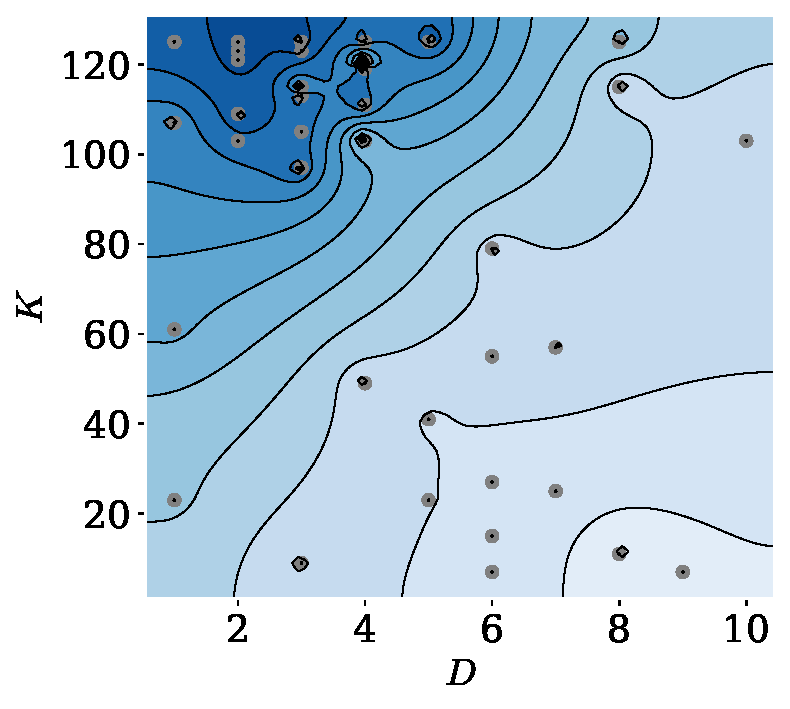
\includegraphics[width=0.33\linewidth,height=3.4cm]{Figures/contour_D_vs_K-9.pdf}} \hfill
\subfloat[$D'$ vs. $K$]{%
  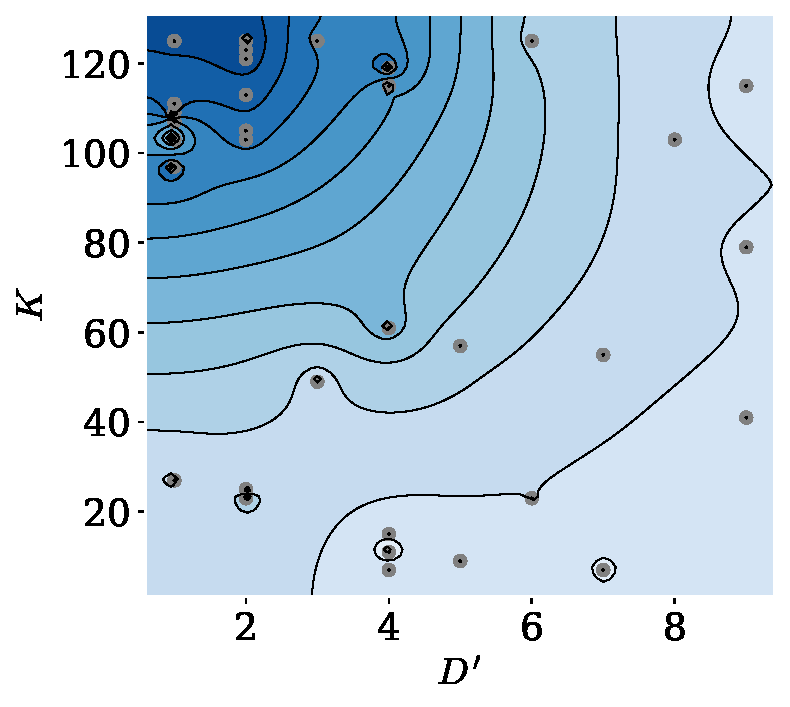
\includegraphics[width=0.33\linewidth,height=3.4cm]{Figures/contour_Dprime_vs_K-9.pdf}} \hfill
\subfloat[$D$ vs. $\mu$]{%
  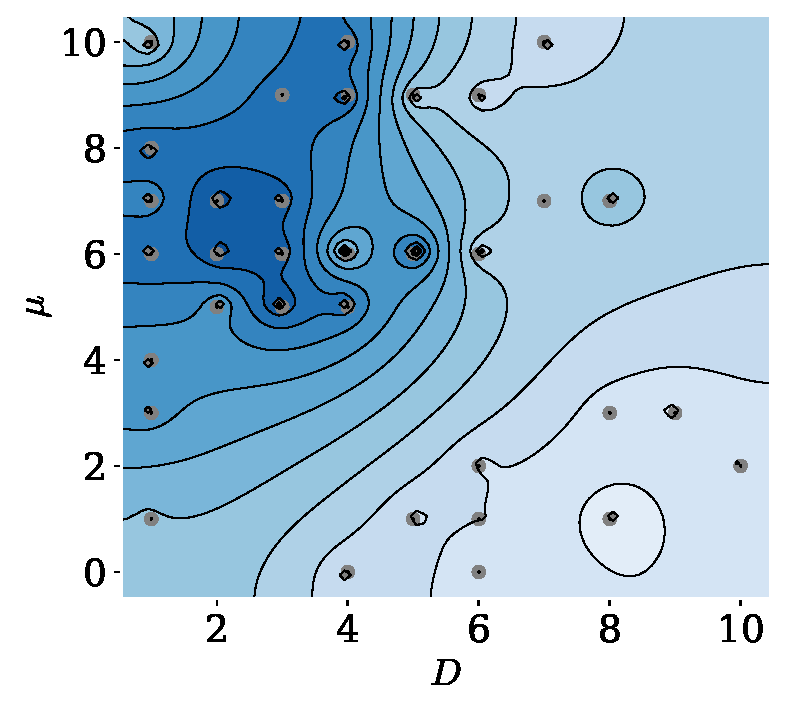
\includegraphics[width=0.33\linewidth,height=3.4cm]{Figures/contour_D_vs_mu-9.pdf}} \\[0.6em]

% --------- FILA 2 ----------
\subfloat[$D'$ vs. $\mu$]{%
  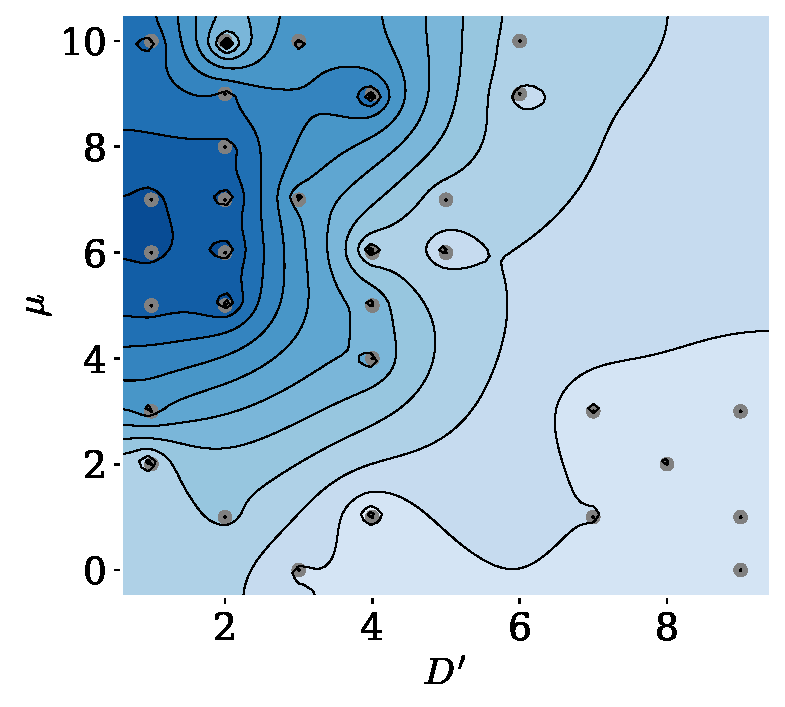
\includegraphics[width=0.33\linewidth,height=3.4cm]{Figures/contour_Dprime_vs_mu-9.pdf}} \hfill
\subfloat[$\tau$ vs. $\mu$]{%
  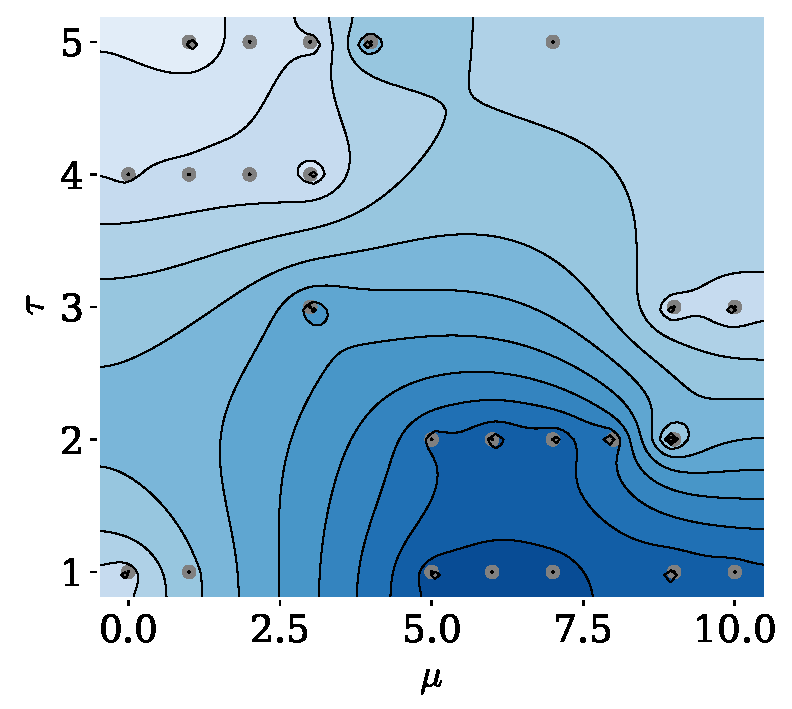
\includegraphics[width=0.33\linewidth,height=3.4cm]{Figures/contour_mu_vs_tau-9.pdf}} \hfill
\subfloat[$D'$ vs. $D$]{%
  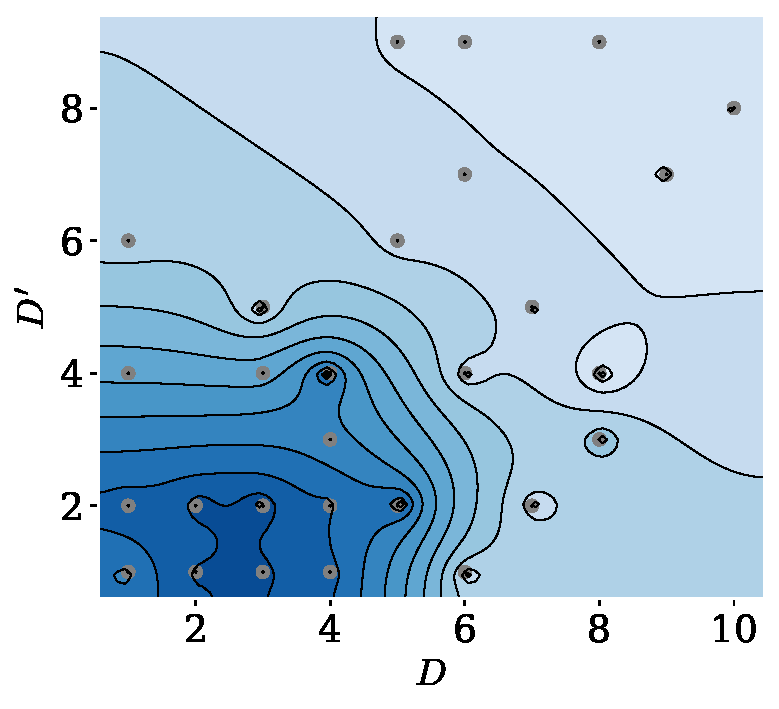
\includegraphics[width=0.33\linewidth,height=3.4cm]{Figures/contour_D_vs_Dprime-9.pdf}} \\[0.8em]

% ================= COLORBAR =================
\begin{tikzpicture}
\begin{axis}[
  hide axis,
  scale only axis,
  width=\linewidth,
  height=0pt,
  colormap name=optunablues,
  colorbar horizontal,
  point meta min=44,
  point meta max=100,
  colorbar style={
    width=\linewidth,
    height=3mm,
    xtick={44, 52, 60, 68, 76, 84, 92, 100},
    xticklabel style={font=\scriptsize},
    xlabel={val accuracy (\%)},
    xlabel style={font=\scriptsize, yshift=2pt},
    scaled ticks=false,
    /pgf/number format/fixed,
    /pgf/number format/precision=1
  }
]
\addplot[draw=none] coordinates {(0,0)};
\end{axis}
\end{tikzpicture}

\end{minipage}%
}

\caption{{Contour plots of validation accuracy (\%) as a function of selected hyperparameter pairs for the highest-performing subject (Subject~9) on the BCI Competition IV-2a dataset. All panels share the same color scale, allowing direct visual comparison across hyperparameter pairs within the subject.}}
\label{fig:global_freq_sbj9}
\end{figure}

{In contrast, for the low-performing subject (Subject~2), the contour surfaces in \Cref{fig:global_freq_sbj2} reveal a markedly less structured and more fragmented hyperparameter--performance landscape.}

%----------------------------------------------------
{For Subject~9, the contour surfaces in \Cref{fig:global_freq_sbj9} exhibit well-defined and relatively smooth high-accuracy regions, suggesting a structured optimization landscape. The panels involving the temporal kernel size $K$ show that the best validation accuracies are concentrated at large kernel values, especially when combined with low-to-moderate embedding orders $D$ and $D'$. This indicates that, for this subject, broader temporal filtering is beneficial as long as the reconstructed state-space dimensionality remains controlled. Similarly, the contours involving the interaction delay $\mu$ show favorable regions for intermediate-to-high delay values, mainly when $D$ and $D'$ remain within lower ranges. The $\mu$--$\tau$ surface further suggests that high performance is preserved for small stride values, particularly around $\tau=1$ or $\tau=2$, combined with moderate-to-large delays. Overall, Subject~9 presents compact but coherent high-performance regions, indicating that \gls{tektenet} can exploit a stable temporal-connectivity structure for this participant, provided that the temporal receptive field, delay, and embedding orders are properly balanced, which is consistent with delay-coordinate reconstruction and transfer-entropy-based modeling of nonlinear directed interactions~\cite{schreiber2000measuring}.}

%----------------------------------------------------
\begin{figure}[H]
\centering

\makebox[\textwidth][c]{%
\begin{minipage}[c]{0.99\textwidth}
\centering

% --------- FILA 1 ----------
\subfloat[$D$ vs. $K$]{%
  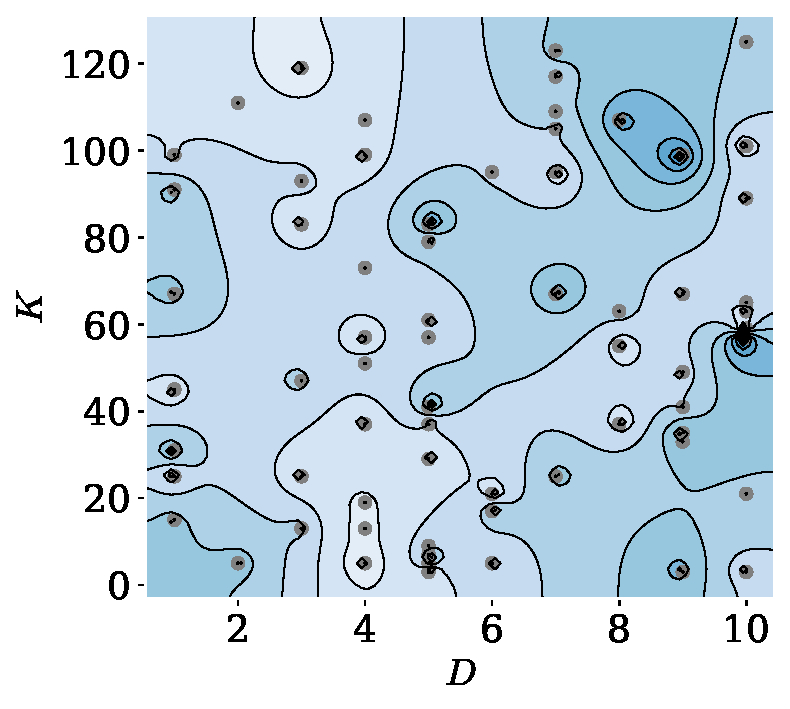
\includegraphics[width=0.33\linewidth,height=3.4cm]{Figures/contour_D_vs_K-2.pdf}} 
\subfloat[$D'$ vs. $K$]{%
  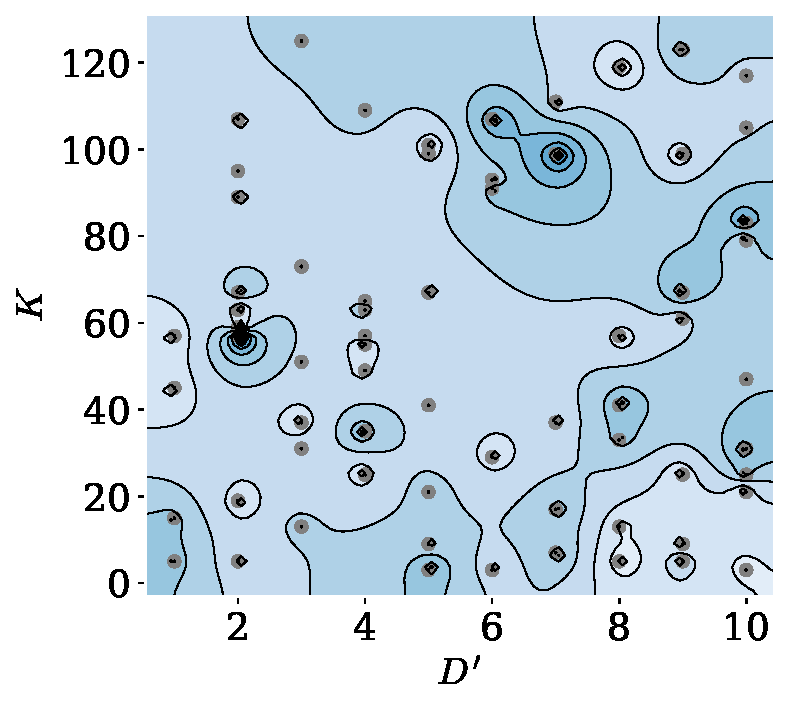
\includegraphics[width=0.33\linewidth,height=3.4cm]{Figures/contour_Dprime_vs_K-2.pdf}} 
\subfloat[$D$ vs. $\mu$]{%
  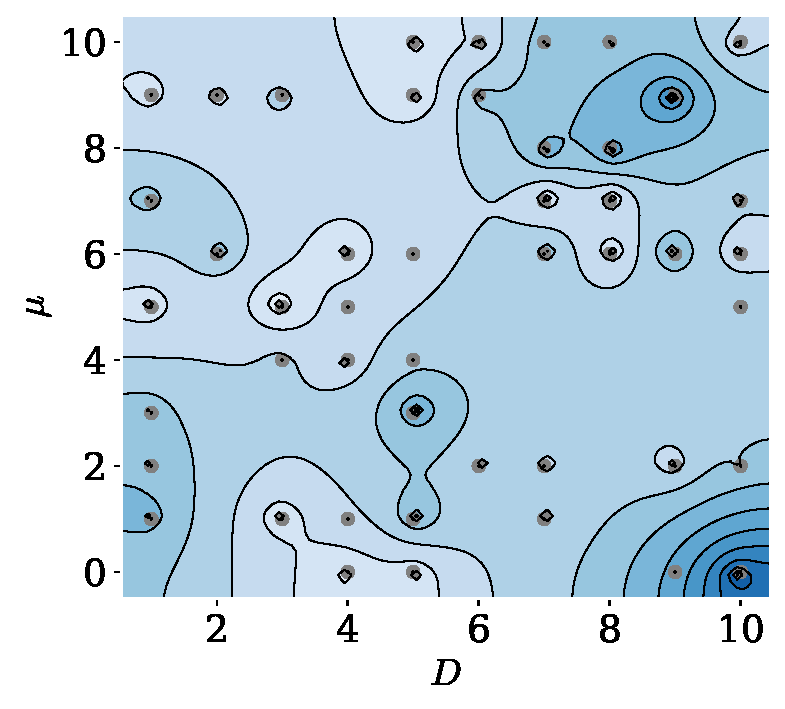
\includegraphics[width=0.33\linewidth,height=3.4cm]{Figures/contour_D_vs_mu-2.pdf}} \\[0.6em]

% --------- FILA 2 ----------
\subfloat[$D'$ vs. $\mu$]{%
  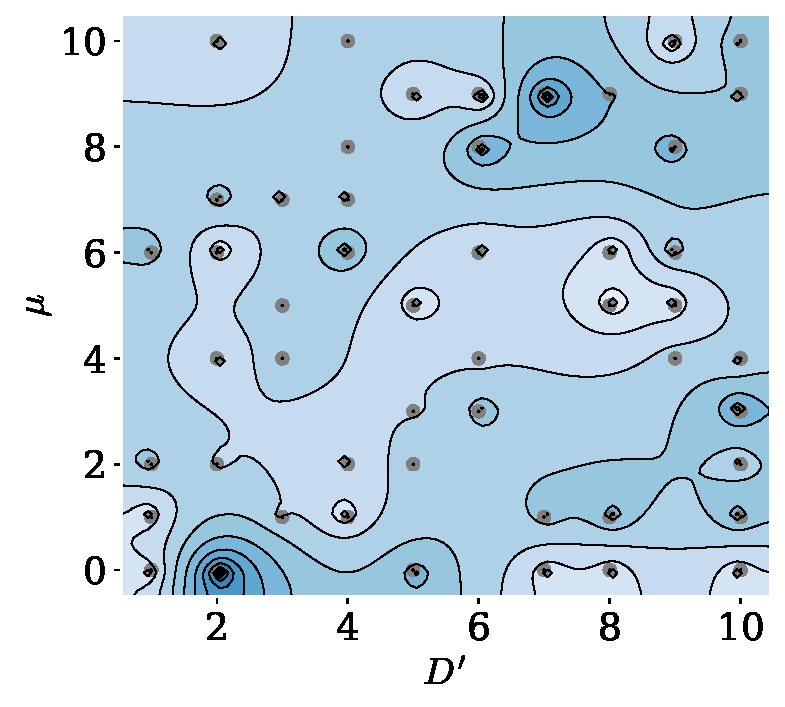
\includegraphics[width=0.33\linewidth,height=3.4cm]{Figures/contour_Dprime_vs_mu-2.pdf}} 
\subfloat[$\tau$ vs. $\mu$]{%
  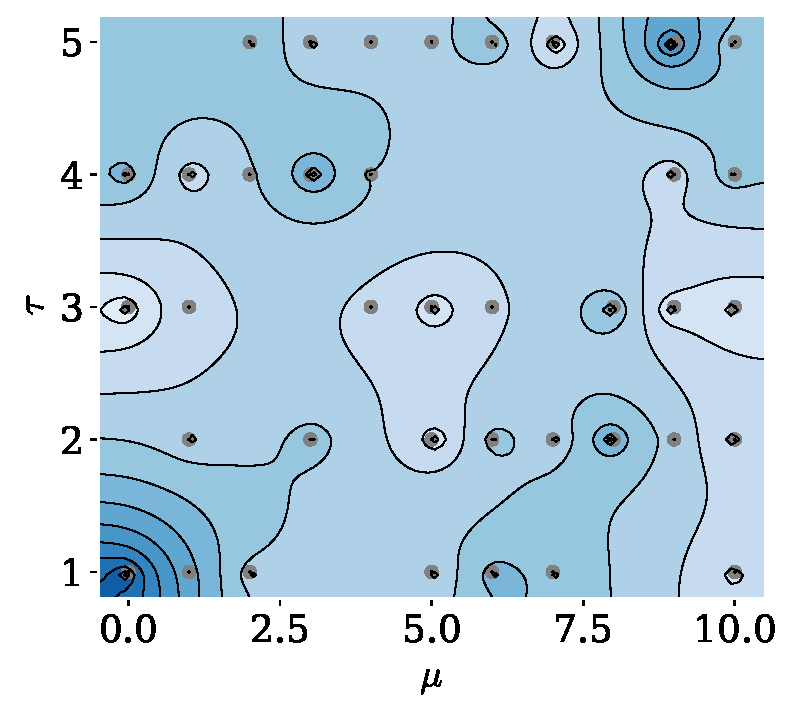
\includegraphics[width=0.33\linewidth,height=3.4cm]{Figures/contour_mu_vs_tau-2.pdf}} 
\subfloat[$D'$ vs. $D$]{%
  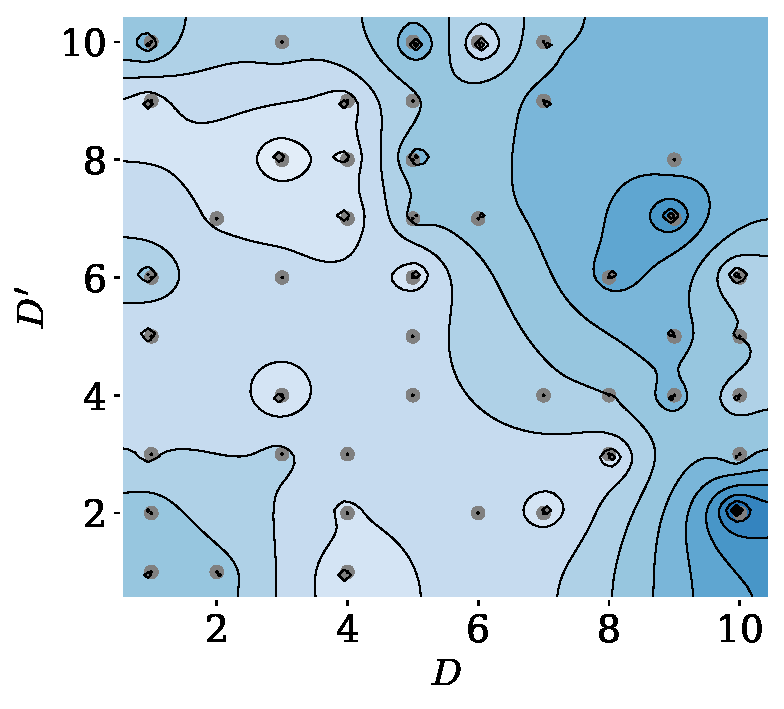
\includegraphics[width=0.33\linewidth,height=3.4cm]{Figures/contour_D_vs_Dprime-2.pdf}} \\[0.8em]

% ================= COLORBAR =================
\begin{tikzpicture}
\begin{axis}[
  hide axis,
  scale only axis,
  width=\linewidth,
  height=0pt,
  colormap name=optunablues,
  colorbar horizontal,
  point meta min=48,
  point meta max=69,
  colorbar style={
    width=\linewidth,
    height=3mm,
    xtick={48, 51, 54, 57, 60, 63, 66, 69},
    xticklabel style={font=\scriptsize},
    xlabel={val accuracy (\%)},
    xlabel style={font=\scriptsize, yshift=2pt},
    scaled ticks=false,
    /pgf/number format/fixed,
    /pgf/number format/precision=1
  }
]
\addplot[draw=none] coordinates {(0,0)};
\end{axis}
\end{tikzpicture}

\end{minipage}%
}

\caption{{Contour plots of validation accuracy (\%) as a function of selected hyperparameter pairs for the lowest-performing subject (Subject~2) on the BCI Competition IV-2a dataset. All panels share the same color scale, allowing direct visual comparison across hyperparameter pairs within the subject.}}
\label{fig:global_freq_sbj2}
\end{figure}
%----------------------------------------------------

{Unlike Subject~9, where high-accuracy regions appear more coherent and localized within specific parameter ranges, Subject~2 exhibits scattered regions of moderate performance distributed across the search space, with no clearly dominant high-performance plateau. This behavior is particularly evident in the panels involving the temporal kernel size $K$, where validation accuracy does not consistently improve for a specific range of kernel values, suggesting that broader temporal filtering alone is not sufficient to stabilize the decoding performance for this subject. Similarly, the contours involving $\mu$, $D$, and $D'$ show abrupt transitions between neighboring regions, indicating that small variations in the interaction delay or embedding dimensionality can substantially modify the reconstructed state-space representation. The $\mu$--$\tau$ surface also presents isolated regions of improved accuracy, reinforcing the idea that the temporal alignment between delayed coordinates is less stable for this participant. Overall, Subject~2 exhibits a less organized optimization landscape, consistent with its lower decoding performance and suggesting that \gls{tektenet} has greater difficulty extracting stable and discriminative temporal-connectivity patterns for this subject. This behavior is aligned with previous reports on inter-subject variability and BCI illiteracy in motor-imagery decoding~\cite{roy2020deep,ashburner2011multivariate}.}
%----------------------------------------------------
\begin{figure}[H]
    \centering
    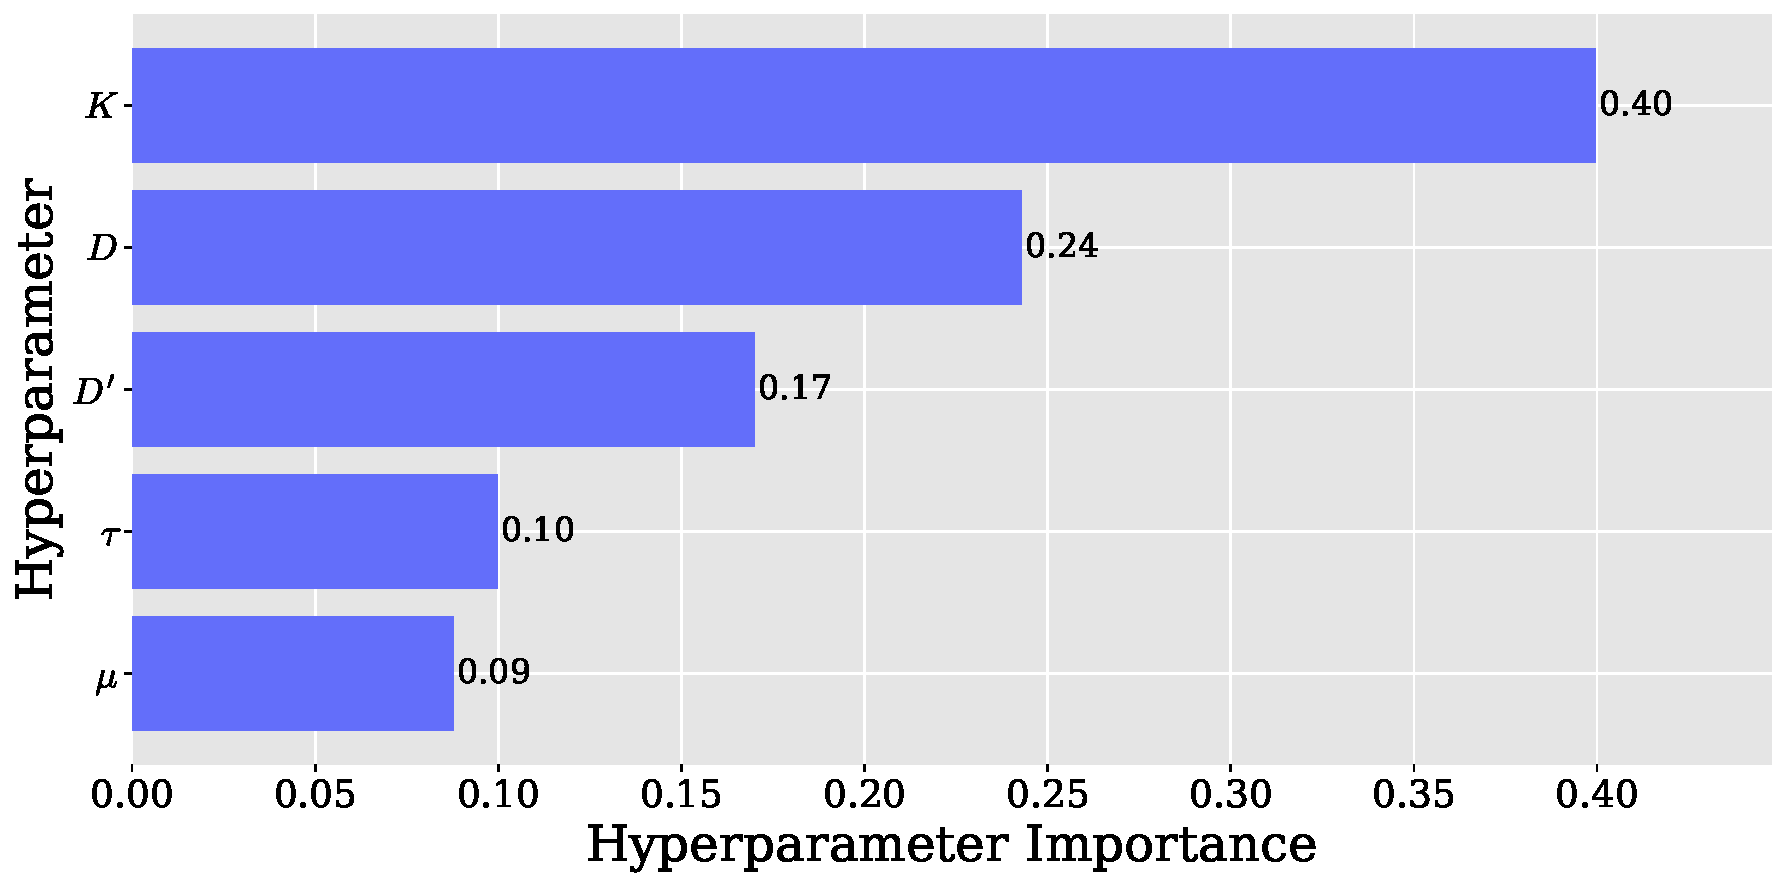
\includegraphics[width=0.8\linewidth]{Figures/optuna_fanova_param_importances_tekte-bci2a.pdf}
    \caption{{Global hyperparameter importance analysis for \gls{tektenet} on the BCI Competition IV-2a dataset. Importance scores quantify the relative contribution of the temporal kernel size $K$, embedding orders $D$ and $D'$, stride $\tau$, and interaction delay $\mu$ to validation accuracy.}}
    \label{fig:fanova_tekte_bci2a}
\end{figure}
%----------------------------------------------------
{To complement the subject-specific contour analysis, a global hyperparameter-importance analysis was conducted to quantify the relative contribution of each \gls{tektenet} hyperparameter to validation accuracy across the explored configurations. As shown in \Cref{fig:fanova_tekte_bci2a}, the temporal convolutional kernel size $K$ exhibits the highest importance score, indicating that the temporal receptive field is the dominant factor influencing model performance on the BCI Competition IV-2a dataset. This result suggests that the ability of \gls{tektenet} to extract informative temporal patterns before the Takens embedding stage is critical for subsequent directed-connectivity estimation.}

{The embedding orders also play an important role, with $D$ and $D'$ ranking as the second and third most influential hyperparameters, respectively. This finding indicates that the dimensionality of the reconstructed state space has a substantial effect on decoding performance, since it determines how much past information from the driving and responding channels is incorporated into the transfer entropy estimation~\cite{schreiber2000measuring}. In contrast, the stride $\tau$ and the interaction delay $\mu$ show lower global importance scores. However, this does not imply that these parameters are irrelevant; rather, their effects appear to be more localized and interaction-dependent, as observed in the contour plots and OAT analysis. Overall, these results indicate that \gls{tektenet} performance is mainly governed by the temporal filtering scale and the Takens embedding dimensionality, while delay and stride contribute more subtly by modulating temporal alignment between reconstructed trajectories, which is consistent with delay-coordinate reconstruction and transfer-entropy-based modeling of nonlinear directed interactions~\cite{Vicente2011,faes2011information}.}

\subsubsection{Interpretability Analysis}

For assessing model interpretability, a subject-specific analysis was conducted across temporal, spatial, and spectral axes. The temporal analysis employs a sliding-window approach for understanding time engagement and training/testing variations. On the spatial axis, the activated TE aims at interpreting functional connectivity patterns. The spectral analysis of channel-wise learned filters focuses on understanding frequency specialization. All analyses were performed under the optimized hyperparameters summarized in~\Cref{tab:hyperparameters_sorted}.

Sliding window analysis enables the exploration of MI engagement variability by examining the temporal evolution of classification accuracy. \Cref{fig:accuracy_all_subjects} presents the attained accuracy as a two-second window is slid along the trials (from 0 to 7 seconds), with subjects sorted according to their performance in~\Cref{fig:accuracy_r3}. At first glance, consistent peak classification accuracies appear within the time window between 2 and 4 seconds after the task onset. Previous studies have demonstrated that this window range suitably captures the most discriminative MI-related patterns by effectively reflecting the {temporal evolution of MI-related sensorimotor rhythms during the active motor-imagery period}~\cite{Gaur2021SlidingWindowCSP}.

  %-------------------------------------------------------------
\setlength\figurewidth{0.38\columnwidth}
\setlength\figureheight{0.3\columnwidth}
\begin{figure}[ht!]
  \centering
  %-------------------------------------------------------------
  \subfloat[\centering Subject 9]{\begin{tikzpicture}
      \begin{axis}[
        width=\figurewidth,
        height=\figureheight,
        ylabel={Accuracy (\%)},
        xlabel={Time window center ($s$)},
        xmin=1, xmax=11, ymin=30, ymax=100,
        xtick={1,...,11},
        xticklabels={1,1.5,2,2.5,3,3.5,4,4.5,5,5.5,6},
        tick pos=bottom,     
        tick label style={font=\footnotesize},
        xlabel style={font=\footnotesize},
        ylabel style={font=\footnotesize},
        minor tick num=0,
        legend style={at={(0.97,0.03)},anchor=south east,font=\footnotesize},
        legend cell align=left,
      ]
       
        \addplot[
          tabblue,
          mark=*,
          mark options={draw=tabblue,fill=tabblue},
          thick,
        ] coordinates {
          (1,58.62) (2,56.03) (3,63.79) (4,82.76) (5,99.14)
          (6,97.41) (7,84.48) (8,57.76) (9,50.00) (10,48.28)
          (11,43.10)
        };
        % \addlegendentry{Training}
        \addplot[
          taborange,
          mark=*,
          mark options={draw=taborange,fill=taborange},
          thick,
        ] coordinates {
          (1,50.00) (2,47.69) (3,51.54) (4,61.54) (5,87.69)
          (6,83.85) (7,84.62) (8,75.38) (9,72.31) (10,70.00)
          (11,62.31)
        };
        % \addlegendentry{Test}
      \end{axis}
    \end{tikzpicture}}
  \subfloat[\centering Subject 8]{    \begin{tikzpicture}
      \begin{axis}[
        width=\figurewidth,
        height=\figureheight,
        % ylabel={Accuracy (\%)},
        yticklabels=\empty,
        xlabel={Time window center ($s$)},
        xmin=1, xmax=11, ymin=30, ymax=100,
        xtick={1,...,11},
        xticklabels={1,1.5,2,2.5,3,3.5,4,4.5,5,5.5,6},
        tick pos=bottom, 
        tick label style={font=\footnotesize},
        xlabel style={font=\footnotesize}, ylabel style={font=\footnotesize},
        minor tick num=1,
        minor tick num=0,
        legend style={at={(0.97,0.03)},anchor=south east,font=\footnotesize},
        legend cell align=left,
      ]
        \addplot[
          tabblue,
          mark=*,
          mark options={draw=tabblue,fill=tabblue},
          thick,
        ] coordinates {
          (1,53.03) (2,55.30) (3,73.48) (4,89.39) (5,99.00)
          (6,94.70) (7,85.61) (8,78.03) (9,77.27) (10,73.48)
          (11,65.91)
        };
        % \addlegendentry{Training}
         \addplot[
          taborange,
          mark=*,
          mark options={draw=taborange,fill=taborange},
          thick,
        ] coordinates {
          (1,50.75) (2,47.01) (3,68.66) (4,81.34) (5,91.79)
          (6,88.81) (7,79.85) (8,76.12) (9,70.15) (10,67.91)
          (11,58.96)
        };
        % \addlegendentry{Test}
      \end{axis}
    \end{tikzpicture}}
  \subfloat[\centering Subject 3]{    \begin{tikzpicture}
      \begin{axis}[
        width=\figurewidth,
        height=\figureheight,
        % ylabel={Accuracy (\%)},
        yticklabels=\empty,
        xlabel={Time window center ($s$)},
        xmin=1, xmax=11, ymin=30, ymax=100,
        xtick={1,...,11},
        xticklabels={1,1.5,2,2.5,3,3.5,4,4.5,5,5.5,6},
        tick pos=bottom, 
        tick label style={font=\footnotesize},
        xlabel style={font=\footnotesize}, ylabel style={font=\footnotesize},
        minor tick num=1,
        minor tick num=0,
        legend style={at={(0.97,0.03)},anchor=south east,font=\footnotesize},
        legend cell align=left,
      ]
        \addplot[
          tabblue,
          mark=*,
          mark options={draw=tabblue,fill=tabblue},
          thick,
        ] coordinates {
          (1, 51.82) (2, 56.93) (3, 64.23) (4, 76.64) (5, 94.16) 
          (6, 89.05) (7, 91.97) (8, 85.40) (9, 81.75) (10, 78.10) 
          (11, 75.91)
        };
        % \addlegendentry{Training}
         \addplot[
          taborange,
          mark=*,
          mark options={draw=taborange,fill=taborange},
          thick,
        ] coordinates {
          (1, 51.82) (2, 59.85) (3, 64.96) (4, 76.64) (5, 90.51) 
          (6, 90.51) (7, 84.67) (8, 82.48) (9, 72.99) (10, 76.64) 
          (11, 67.88)
        };
        % \addlegendentry{Test}
      \end{axis}
    \end{tikzpicture}}\\
  %-------------------------------------------------------------
  \subfloat[\centering Subject 1]{    \begin{tikzpicture}
      \begin{axis}[
        width=\figurewidth,
        height=\figureheight,
        ylabel={Accuracy (\%)},
        % yticklabels=\empty,
        xlabel={Time window center ($s$)},
        xmin=1, xmax=11, ymin=30, ymax=100,
        xtick={1,...,11},
        xticklabels={1,1.5,2,2.5,3,3.5,4,4.5,5,5.5,6},
        tick pos=bottom,
        tick label style={font=\footnotesize},
        xlabel style={font=\footnotesize}, ylabel style={font=\footnotesize},
        minor tick num=1,
        minor tick num=0,
        legend style={at={(0.97,0.03)},anchor=south east,font=\footnotesize},
        legend cell align=left,
      ]
        \addplot[
          tabblue,
          mark=*,
          mark options={draw=tabblue,fill=tabblue},
          thick,
        ] coordinates {
          (1,47.37) (2,52.63) (3,81.20) (4,86.47) (5,90.98)
          (6,78.20) (7,66.17) (8,54.14) (9,54.89) (10,53.38)
          (11,51.13)
        };
        % \addlegendentry{Training}
        \addplot[
          taborange,
          mark=*,
          mark options={draw=taborange,fill=taborange},
          thick,
        ] coordinates {
          (1,52.14) (2,50.71) (3,58.57) (4,62.86) (5,62.86)
          (6,57.14) (7,52.14) (8,46.43) (9,54.29) (10,45.71)
          (11,55.00)
        };
        % \addlegendentry{Test}
      \end{axis}
    \end{tikzpicture}
}
  \subfloat[\centering Subject 7]{    \begin{tikzpicture}
      \begin{axis}[
        width=\figurewidth,
        height=\figureheight,
        % ylabel={Accuracy (\%)},
        yticklabels=\empty,
        xlabel={Time window center ($s$)},
        xmin=1, xmax=11, ymin=30, ymax=100,
        xtick={1,...,11},
        xticklabels={1,1.5,2,2.5,3,3.5,4,4.5,5,5.5,6},
        tick pos=bottom, 
        tick label style={font=\footnotesize},
        xlabel style={font=\footnotesize}, ylabel style={font=\footnotesize},
        minor tick num=1,
        minor tick num=0,
        legend style={at={(0.97,0.03)},anchor=south east,font=\footnotesize},
        legend cell align=left,
      ]
        \addplot[
          tabblue,
          mark=*,
          mark options={draw=tabblue,fill=tabblue},
          thick,
        ] coordinates {
          (1,52.17) (2,47.83) (3,68.84) (4,80.43) (5,92.75)
          (6,78.99) (7,65.22) (8,62.32) (9,57.97) (10,62.32)
          (11,55.80)

        };
        % \addlegendentry{Training}
        \addplot[
          taborange,
          mark=*,
          mark options={draw=taborange,fill=taborange},
          thick,
        ] coordinates {
         (1,45.39) (2,46.10) (3,65.25) (4,71.63) (5,77.30)
         (6,70.92) (7,66.67) (8,63.83) (9,59.57) (10,62.41)
         (11,59.57)
          
        };
        % \addlegendentry{Test}
      \end{axis}
    \end{tikzpicture}
}
  \subfloat[\centering Subject 5]{    \begin{tikzpicture}
      \begin{axis}[
        width=\figurewidth,
        height=\figureheight,
        % ylabel={Accuracy (\%)},
        yticklabels=\empty,
        xlabel={Time window center ($s$)},
        xmin=1, xmax=11, ymin=30, ymax=100,
        xtick={1,...,11},
        xticklabels={1,1.5,2,2.5,3,3.5,4,4.5,5,5.5,6},
        tick pos=bottom, 
        tick label style={font=\footnotesize},
        xlabel style={font=\footnotesize}, ylabel style={font=\footnotesize},
        minor tick num=1,
        minor tick num=0,
        legend style={at={(0.97,0.03)},anchor=south east,font=\footnotesize},
        legend cell align=left,
      ]
        \addplot[
          tabblue,
          mark=*,
          mark options={draw=tabblue,fill=tabblue},
          thick,
        ] coordinates {
          (1,52.71) (2,53.49) (3,53.49) (4,53.49) (5,96.90)
          (6,54.26) (7,58.14) (8,58.14) (9,53.49) (10,51.94)
          (11,48.84)
        };
        % \addlegendentry{Training}
        \addplot[
          taborange,
          mark=*,
          mark options={draw=taborange,fill=taborange},
          thick,
        ] coordinates {
         (1,48.15) (2,52.59) (3,40.74) (4,51.11) (5,65.93)
         (6,54.81) (7,51.11) (8,48.89) (9,45.19) (10,45.93)
         (11,48.15)
        };
        % \addlegendentry{Test}
      \end{axis}
    \end{tikzpicture}}\hfill
  %-------------------------------------------------------------
  \subfloat[\centering Subject 4]{    \begin{tikzpicture}
      \begin{axis}[
        width=\figurewidth,
        height=\figureheight,
        % ylabel={Accuracy (\%)},
        ylabel={Accuracy (\%)},
        xlabel={Time window center ($s$)},
        xmin=1, xmax=11, ymin=30, ymax=100,
        xtick={1,...,11},
        xticklabels={1,1.5,2,2.5,3,3.5,4,4.5,5,5.5,6},
        tick pos=bottom, 
        tick label style={font=\footnotesize},
        xlabel style={font=\footnotesize}, ylabel style={font=\footnotesize},
        minor tick num=1,
        minor tick num=0,
        legend style={at={(0.97,0.03)},anchor=south east,font=\footnotesize},
        legend cell align=left,
      ]
        \addplot[
          tabblue,
          mark=*,
          mark options={draw=tabblue,fill=tabblue},
          thick,
        ] coordinates {
          (1,41.59) (2,58.41) (3,54.87) (4,61.95) (5,94.69)
          (6,57.52) (7,46.90) (8,49.56) (9,48.67) (10,57.52)
          (11,54.87)
        };
        % \addlegendentry{Training}
        \addplot[
          taborange,
          mark=*,
          mark options={draw=taborange,fill=taborange},
          thick,
        ] coordinates {
          (1,47.22) (2,51.85) (3,43.52) (4,53.70) (5,61.11)
          (6,51.85) (7,49.07) (8,55.56) (9,58.33) (10,51.85)
          (11,51.85)
        };
        % \addlegendentry{Test}
      \end{axis}
    \end{tikzpicture}}
  \subfloat[\centering Subject 2]{    \begin{tikzpicture}
      \begin{axis}[
        width=\figurewidth,
        height=\figureheight,
        yticklabels=\empty,
        % ylabel={Accuracy (\%)},
        xlabel={Time window center ($s$)},
        xmin=1, xmax=11, ymin=30, ymax=100,
        xtick={1,...,11},
        xticklabels={1,1.5,2,2.5,3,3.5,4,4.5,5,5.5,6},
        tick pos=bottom,
        tick label style={font=\footnotesize},
        xlabel style={font=\footnotesize}, ylabel style={font=\footnotesize},
        minor tick num=1,
        minor tick num=0,
        legend style={at={(0.97,0.03)},anchor=south east,font=\footnotesize},
        legend cell align=left,
      ]
        \addplot[
          tabblue,
          mark=*,
          mark options={draw=tabblue,fill=tabblue},
          thick,
        ] coordinates {
          (1,53.49) (2,60.47) (3,64.34) (4,58.91) (5,51.94)
          (6,43.41) (7,48.06) (8,53.49) (9,51.16) (10,47.29)
          (11,48.84)
        };
        % \addlegendentry{Training}
        \addplot[
          taborange,
          mark=*,
          mark options={draw=taborange,fill=taborange},
          thick,
        ] coordinates {
          (1,49.14) (2,45.69) (3,52.59) (4,55.17) (5,64.66)
          (6,55.17) (7,50.00) (8,56.03) (9,52.59) (10,51.72)
          (11,46.55)
        };
        % \addlegendentry{Test}
      \end{axis}
    \end{tikzpicture}}
  \subfloat[\centering Subject 6]{    \begin{tikzpicture}
      \begin{axis}[
        width=\figurewidth,
        height=\figureheight,
        yticklabels=\empty,
        xlabel={Time window center ($s$)},
        xmin=1, xmax=11, ymin=30, ymax=100,
        xtick={1,...,11},
        xticklabels={1,1.5,2,2.5,3,3.5,4,4.5,5,5.5,6},
        tick pos=bottom,
        tick label style={font=\footnotesize},
        xlabel style={font=\footnotesize}, 
        ylabel style={font=\footnotesize},
        minor tick num=1,
        minor tick num=0,
        legend style={anchor=north east,font=\footnotesize},
        legend cell align=left,
      ]
        \addplot[
          tabblue,
          mark=*,
          mark options={draw=tabblue,fill=tabblue},
          thick,
        ] coordinates {
          (1,44.12) (2,50.00) (3,52.21) (4,53.68) (5,59.56)
          (6,52.21) (7,50.00) (8,46.32) (9,49.26) (10,49.26)
          (11,49.26)
        };
        \addlegendentry{Training}
         \addplot[
         taborange,
          mark=*,
          mark options={draw=taborange,fill=taborange},
          thick,
        ] coordinates {
          (1,52.82) (2,50.70) (3,56.34) (4,59.86) (5,61.97)
          (6,57.75) (7,54.93) (8,50.70) (9,53.52) (10,47.89)
          (11,43.66)
        };
        \addlegendentry{Test}
      \end{axis}
    \end{tikzpicture}
}
  %-------------------------------------------------------------
  \caption{Classification accuracy for each subject across overlapping time windows during the 7-second \gls{mi} task. A total of 11 time windows were used, each with a 0.5-second overlap. The x-axis represents the center of each time window, and the y-axis shows the classification accuracy (\%). This analysis reveals temporal dynamics in classification performance throughout the \gls{mi} period.}
  \label{fig:accuracy_all_subjects}
\end{figure}
%-------------------------------------------------------------

Furthermore, the temporal performance profiles cluster subjects into three groups. In the group of high-performing subjects (Subjects 9, 8, and 3), \gls{tektenet} exhibited a marked and consistent increase in accuracy of over $90\%$ within the 2–4 second window. Despite the slight decline towards the trial end, the proposed model maintained relatively high test accuracy levels (above $60\%$), suggesting the presence of stable and task-relevant neural activity in these subjects. On subjects 7, 1, and 5 (mid-performing), the proposed model performed moderately, with test accuracy peaking between $60\%$ and $80\%$ within the 2- and 4-second windows. The temporal profile of this group exhibits a clear training-to-test accuracy gap, followed by a gradual decline in training accuracy. Such a profile indicates existing MI-related neural patterns, but these are less consistent and more susceptible to cognitive variability than those in the high-performing group~\cite{duang}. For the group of low-performing subjects (Subjects 6, 4, and 2), the accuracy evolved flatly or with high variability around the chance level (between $45\%$ and $60\%$). Particularly, {Subject~4} presented severe overfitting characterized by an abrupt difference between training and test subsets in the window centered at three seconds. Such an accuracy gap is a symptom of inconsistent or weak MI-related neural patterns, which limit the reliability of classification. Therefore, the temporal performance profiles revealed differences in the quality and steadiness of the neural patterns among subjects, proving the need for subject-dependent MI models.
% %------------------------------------------------------------------------------
\begin{figure}[H]
    \centering
    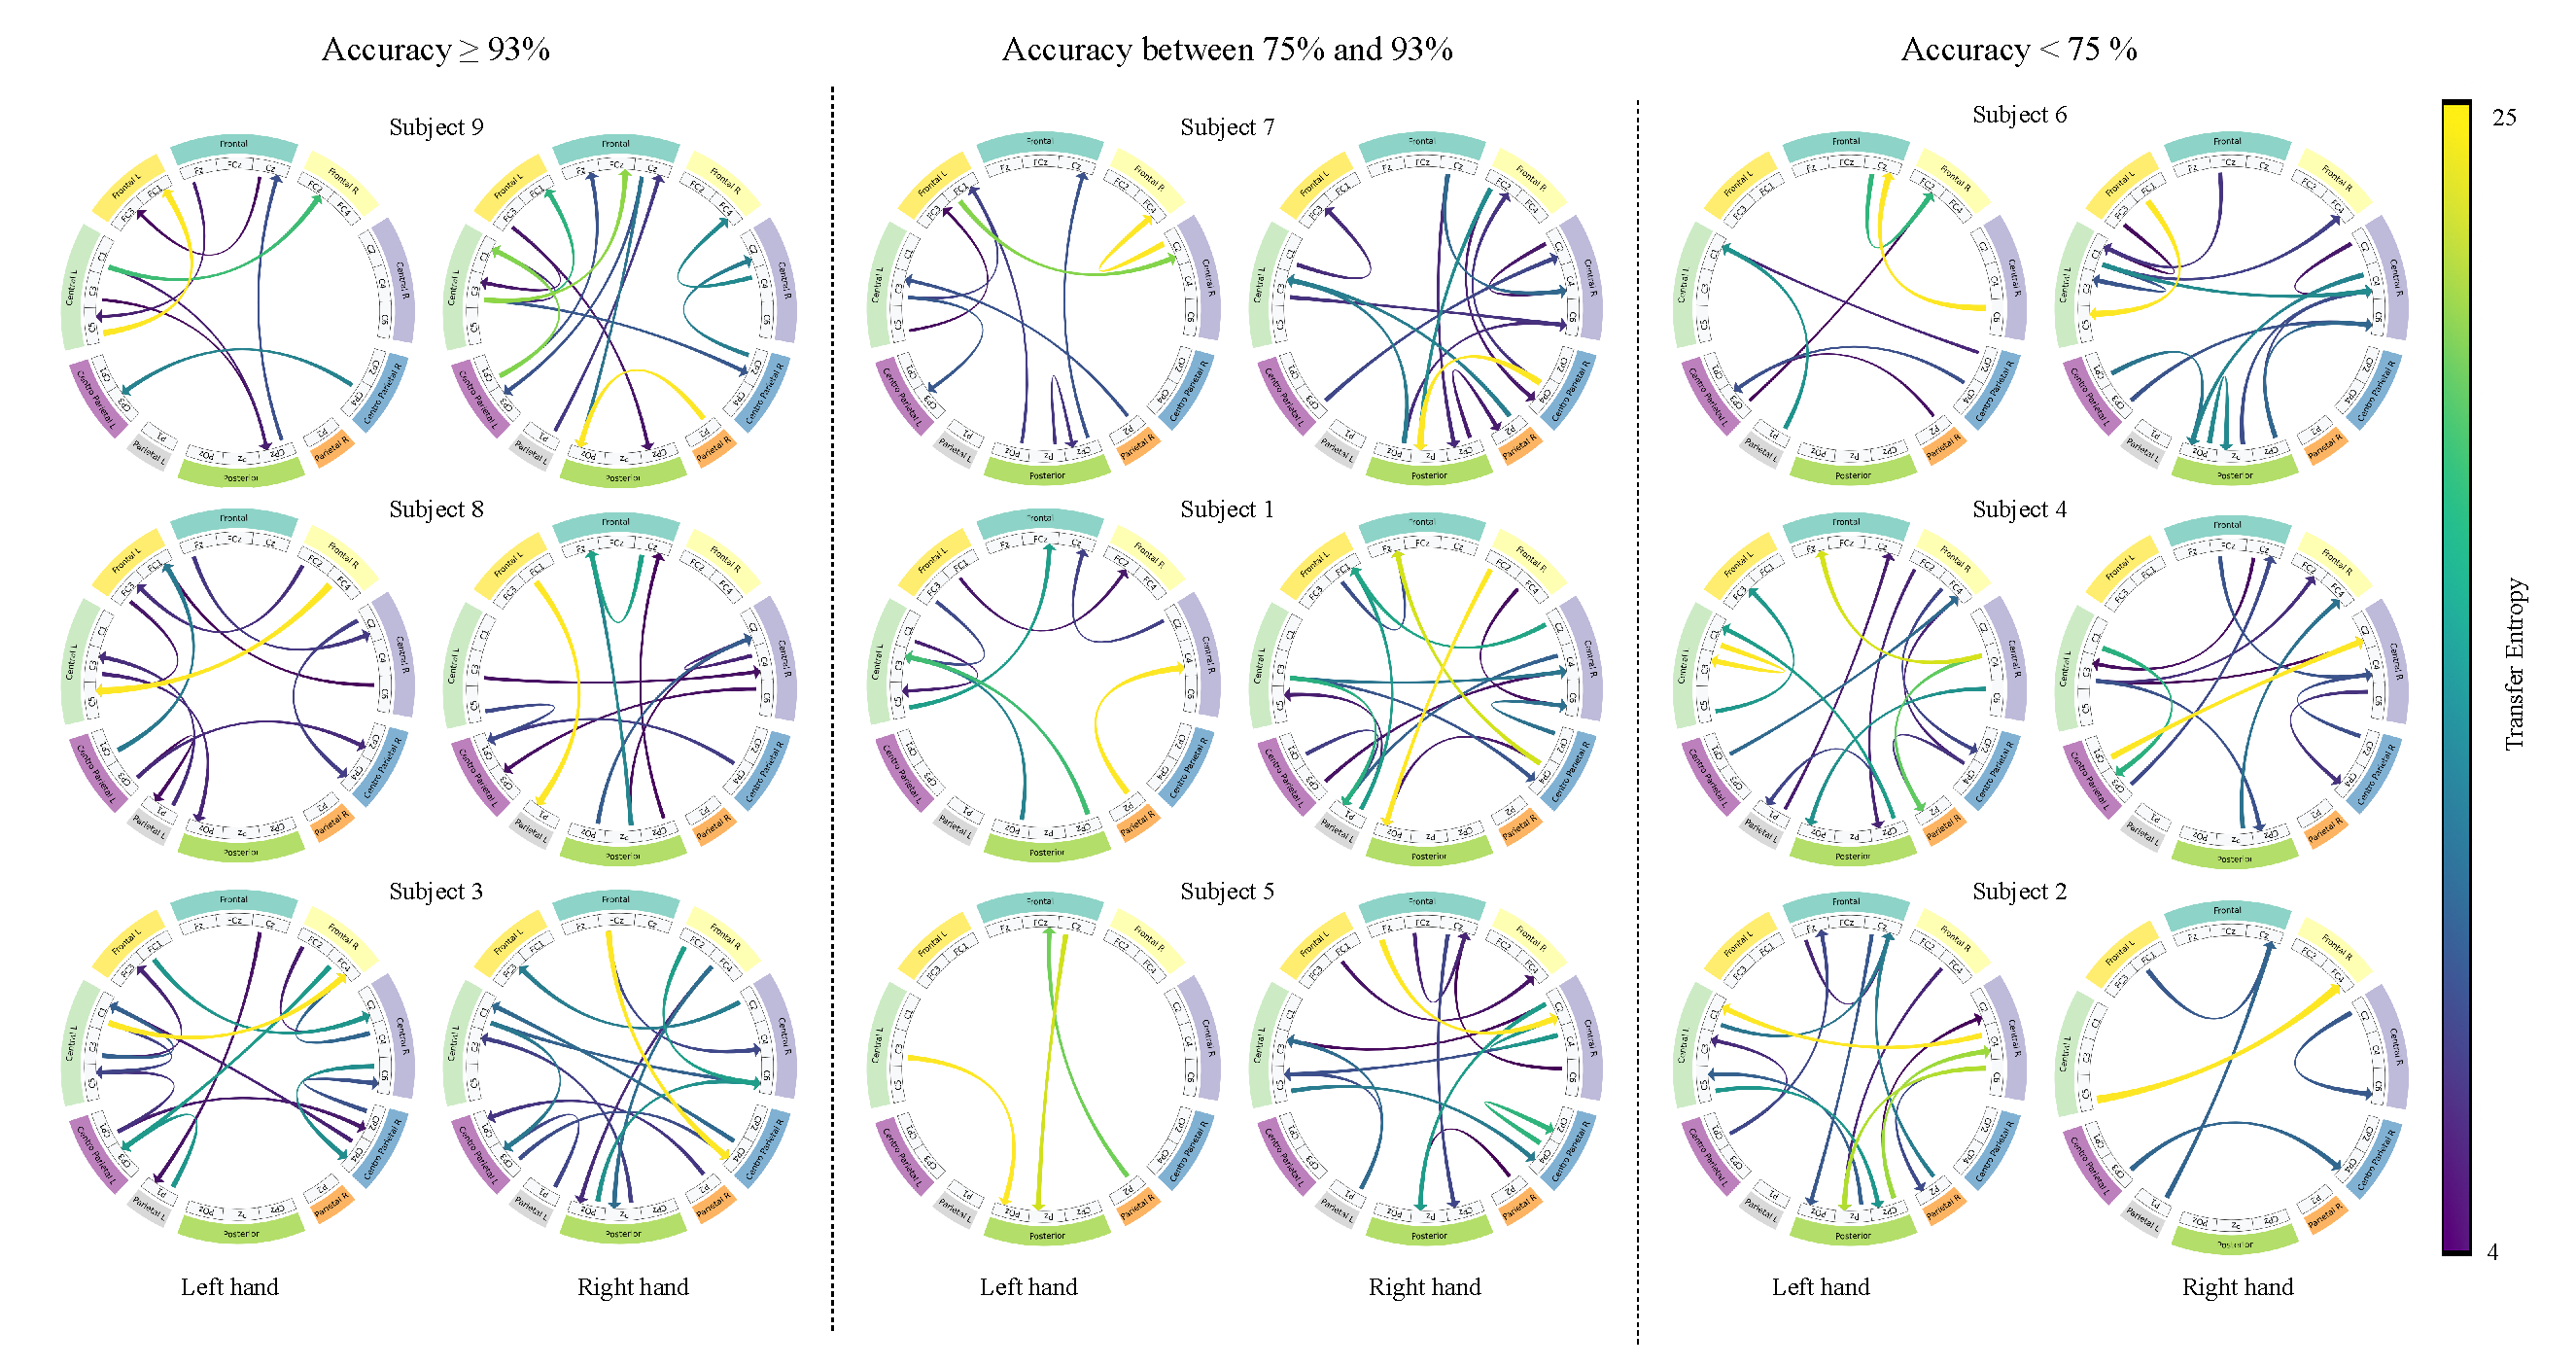
\includegraphics[width=\linewidth]{Figures/Conectivities.pdf}
    \caption{Brain connectivity patterns during left- and right-hand \gls{mi} tasks across models grouped by test accuracy. High performed (accuracy $\geq$ 93\%), mid performed (accuracy between 75\% and 93\%), and low performed (accuracy $<$ 75\%) display distinct activation distributions. Each row corresponds to a representative model within each performed group.}
    \label{fig:conectivitie}
\end{figure}
% %------------------------------------------------------------------------------
For spatial interpretability, the well-established activation maximization technique optimizes the model's output for each \gls{mi} class with respect to the TE layer. This interpretability technique enables the identification of \gls{tektenet} connectivities that strongly contribute to class-specific activations. It also allows for the analysis of the spatial distribution and intensity of interactions between brain regions, providing a clear depiction of the functional dynamics underlying \gls{mi} tasks. 

% %----------------------------------------------------------------------------
\begin{figure}[H]
  \centering

  \makebox[\textwidth]{%
    % --- Columna izquierda: "Channels" ---
    \begin{minipage}[c]{0.08\textwidth}
      \centering
      \rotatebox{90}{\normalsize Channels}
    \end{minipage}%
    \hspace{0.6em}%
    % --- Bloque derecho: paneles + colorbar ---
    \begin{minipage}[c]{0.90\textwidth}
      \centering

      % --- Tamaños (CLAVE: usar \linewidth del minipage) ---
      \newlength{\FW}
      \newlength{\FH}
      \setlength{\FW}{0.32\linewidth}  % <-- 3 por fila
      \setlength{\FH}{0.20\linewidth}

      % ====== Fila 1 ======
      \subfloat[\centering Subject 9]{%
        \includegraphics[width=\FW,height=\FH,keepaspectratio]{Figures/Freqz9.pdf}%
      }\hfill
      \subfloat[\centering Subject 7]{%
        \includegraphics[width=\FW,height=\FH,keepaspectratio]{Figures/Freqz7.pdf}%
      }\hfill
      \subfloat[\centering Subject 6]{%
        \includegraphics[width=\FW,height=\FH,keepaspectratio]{Figures/Freqz6.pdf}%
      }\\[-0.3em]

      % ====== Fila 2 ======
      \subfloat[\centering Subject 8]{%
        \includegraphics[width=\FW,height=\FH,keepaspectratio]{Figures/Freqz8.pdf}%
      }\hfill
      \subfloat[\centering Subject 1]{%
        \includegraphics[width=\FW,height=\FH,keepaspectratio]{Figures/Freqz1.pdf}%
      }\hfill
      \subfloat[\centering Subject 4]{%
        \includegraphics[width=\FW,height=\FH,keepaspectratio]{Figures/Freqz4.pdf}%
      }\\[-0.3em]

      % ====== Fila 3 ======
      \subfloat[\centering Subject 3]{%
        \includegraphics[width=\FW,height=\FH,keepaspectratio]{Figures/Freqz3.pdf}%
      }\hfill
      \subfloat[\centering Subject 5]{%
        \includegraphics[width=\FW,height=\FH,keepaspectratio]{Figures/Freqz5.pdf}%
      }\hfill
      \subfloat[\centering Subject 2]{%
        \includegraphics[width=\FW,height=\FH,keepaspectratio]{Figures/Freqz2.pdf}%
      }

      \vspace{3pt}

      % --- Texto centrado como en tu figura buena ---
      {\small\bfseries Frequency [Hz]}

      \vspace{2pt}

      % ====== Colorbar (viridis, -40..0 dB) ======
      \begin{tikzpicture}
        \begin{axis}[
          hide axis,
          scale only axis,
          width=\linewidth,
          height=0pt,
          colormap/viridis,
          point meta min=-40,
          point meta max=0,
          colorbar,
          colorbar horizontal,
          colorbar sampled,
          colorbar style={
            width=0.92\linewidth,
            height=2mm,
            at={(0.5,0)}, anchor=south,
            xtick={-40,-30,-20,-10,0},
            xticklabel style={font=\scriptsize},
            xlabel={Magnitude [dB]},
            xlabel style={font=\scriptsize, yshift=2pt},
            scaled ticks=false,
          },
        ]
          \addplot [draw=none] coordinates {(0,0)};
        \end{axis}
      \end{tikzpicture}

    \end{minipage}%
  }

  \vspace{2pt}
  \caption{Frequency responses (dB) of the filters learned by the \textit{depthwise} layer. In each panel, the $x$-axis shows frequency (Hz) and the $y$-axis shows the 22 \gls{eeg}channels; the color indicates the average magnitude in dB.}
  \label{fig:frecuencies}
\end{figure}

% %----------------------------------------------------------------------------

\Cref{fig:conectivitie} highlights the directionality, magnitude, and causal nature of the 5\% largest interactions between cortical regions, computed under the \gls{te} framework, across the nine subjects grouped according to their performance in~\Cref{fig:accuracy_r3}. In the high-performing group, causal activation patterns exhibited contralateral connections involving frontal, central, and parietal areas, emphasizing the directionality and magnitude of these connections. For instance, Subject 9 revealed strong paths including $C5\rightarrow FC1$, $C3\rightarrow FCz$, and $P2\rightarrow POz$, while Subject 8 highlighted the $FC4\rightarrow C5$ and $FC1\rightarrow P1$ connections for left and right hand MI, respectively. In the mid-performing subjects, causal interactions are more widespread and less contralateralized than in the previous group, hence partially aligning with MI-related patterns. Remarkably, connections $CP4\rightarrow Fz$ and $FC2\rightarrow POz$, in Subject 1, $C3\rightarrow POz$ and $Cz\rightarrow Pz$, in Subject 5, suggest compensatory recruitment of posterior regions. Conversely, the activations in the low-performing group lack contralateral organization, with atypical interhemispheric causal connections. For instance, the connections between the left-frontal and left-central channels in Subject 6 are atypical in the MI task~\cite{almohammadi2024}. Additionally, the right hemisphere is responsible for most of the highlighted connections in Subjects 2 and 4. Therefore, the spatial and causal interpretation of \gls{tektenet} elucidates the relationship between functional connectivity and \gls{mi} decoding performance, demonstrating efficient sensorimotor integration for the task at hand in the first group~\cite{leeuwis2021functional,vidaurre2020sensorimotor} and the compensatory recruitment of posterior regions in the second group~\cite{angulo2025proficiency}.

The characterization of the spectral behavior of the \gls{tektenet} relies on the frequency response of the channel-wise learned filters for each subject. The frequency response results from the fold-averaged magnitude of the Fast Fourier Transform computed for each convolution kernel. \Cref{fig:frecuencies} presents the resulting magnitude response (in dB) along the frequency (0 to 100Hz) and the channels (from left to right), thereby visually assessing variability among the subject groups and the selectivity of the learned filters across the frequency spectrum.

According to~\Cref{fig:frecuencies}, the proposed model yields a more structured spectral pattern in the high-performing subjects (first column) than in the rest of the cohort. In particular, the filters exhibited a band-pass-like structure in Subjects 3 and 8 around 20Hz, with a slight rightward predominance in Subject 8. From a neurophysiological perspective, the beta band (20 Hz) is associated with sensorimotor coordination and exhibits contralateral lateralization to movement, particularly within the left hemisphere during motor or spatial-orienting tasks~\cite{lasaponara2020pre}. In the case of Subject 9, the filters displayed an unattenuated response around {40 Hz}, primarily concentrated {over right-hemispheric channels}. {This pattern should be interpreted cautiously as a model-derived spectral relevance rather than as direct evidence of a cortical gamma generator, since scalp EEG responses in this frequency range may be influenced by source mixing, volume conduction, residual artifacts, or myogenic contamination~\cite{Whitham2007Scalp}.} Hence, the structured frequency response suggests that the depthwise convolutional filters adapt to preserve the oscillatory components, relevant for the classification task, effectively acting as spectral selectors that maintain frequency regions containing discriminative neural information.

Regarding the second group and third groups (center and right columns), the spectral behavior was less defined compared to the first group. Only the learned filters for Subject 1 partially selected frequencies around 25 Hz over the left hemisphere, similar to the best-performed subjects, albeit with lower clarity and spatial extent. For Subjects 7 and 5, the filters develop a spurious magnitude response, lacking spectral or spatial alignment. Contrarily, the depthwise convolutional filters for the latter group yield an elongated and flat spectral response, reflecting the absence of frequency selectivity. Therefore, the \gls{tektenet}'s spectral specialization positively relates to classification performance, as the low power of MI-related rhythms, particularly beta and gamma, is associated with lower cognitive performance and reduced classification accuracy~\cite{bakhtiari2023power, avital2024cognitive}.

\subsubsection{Performance Assessment}

{This contribution evaluates} \gls{tektenet}'s performance on the official testing set from the BCI Competition IV Dataset 2a. \Cref{tab:metric_results} presents the per-subject performance metrics on this subset, sorted by validation accuracy.

In general, note that the testing accuracy naturally decreased by approximately 7\% compared to the validation one, due to the intrinsic within-subject variability. However, the average F1 score of over 80\% indicates that \gls{tektenet} successfully identified individual \gls{mi} patterns, demonstrating a reasonable generalization capability. For the high-performing group, the model consistently reached scores of over 90\%. Such a result indicates that \gls{tektenet} finds well-structured neurophysiological patterns with both precision and generalizability. For the mid-performing group, \gls{tektenet} yields F1 scores between 75\% and 85\%, followed by the most significant accuracy drops compared to the validation set. Such a finding indicates transitional signal regimes or moderate generalization characteristics, due to accentuated between-session variability. The low-performing group remains just above the chance levels, suggesting highly intrinsic neurophysiological noise or BCI illiteracy. It is also worth mentioning that Subjects 5, 4, and 2 present the most difference between Sensitivity and Specificity, with F1 scores over  65\%, despite the class balance provided by the competition. Hence, the heterogeneity in class distributions emerges as the most reasonable explanation for uneven metrics on such subjects, which facilitates the labeling of the positive class while hindering the negative. Therefore, the stratification and subject-wise analysis highlight the necessity of adaptive or personalized strategies in BCI decoding frameworks, while providing a deeper understanding of the inner workings of \gls{tektenet} across individuals. 
% %----------------------------------------------------------------------------
\begin{table}[H]
\centering
\begin{tabular}{crrrrr}
\toprule
\textbf{Subject} & \textbf{Val. Acc (\%)} & \textbf{Acc. (\%)} & \textbf{F1 (\%)} & \textbf{Sens. (\%)} & \textbf{Spec. (\%)}\\
\midrule
9 & $99.1 \pm 1.9$  & $90.0$  & $90.1$  & $90.8$  & $89.2$\\
8 & $98.5 \pm 2.0$  & $92.5$  & $92.8$  & $94.1$  & $90.9$\\
3 & $94.2 \pm 6.0$  & $93.4$  & $93.9$  & $98.6$  & $88.1$\\
7 & $91.7 \pm 6.9$  & $77.1$  & $78.7$  & $85.5$  & $69.0$\\
1 & $89.9 \pm 8.3$  & $85.1$  & $85.3$  & $87.1$  & $83.1$\\
5 & $88.4 \pm 5.1$  & $74.8$  & $75.0$  & $78.5$  & $71.4$\\
6 & $72.6 \pm 8.4$  & $73.1$  & $71.3$  & $65.5$  & $81.1$\\
4 & $72.3 \pm 13.7$ & $75.0$  & $74.8$  & $75.4$  & $74.6$\\
2 & $67.7 \pm 8.4$  & $59.9$  & $66.7$  & $80.3$  & $39.4$\\
\midrule
\textbf{Avg} & $\mathbf{86.0 \pm 2.5}$ & $\mathbf{80.1}$ & $\mathbf{81.0}$ & $\mathbf{84.0}$ & $\mathbf{76.3}$\\
\bottomrule
\end{tabular} 
\caption{Performance metrics achieved by \gls{tektenet} on the validation and official testing sets. Subjects are sorted in descending order of validation accuracy. Mean and standard deviation for each metric are computed from a five-fold cross-validation.}
\label{tab:metric_results}
\end{table}
%-----------------------------------------------

\Cref{tab:acc_comparisonn} contrasts the proposed \gls{tektenet} against state-of-the-art approaches on the testing sets from the BCI Competition IV in terms of Floating Point Operations (FLOPs), number of trainable parameters (NTP), and average accuracy (color-coded). Both, FLOPs and NTP, describe the computational efficiency and complexity of models, which directly impact performance, scalability, and deployability. Contrasted approaches range from traditional feature engineering techniques (square mark), through deep learning architectures (circle mark), to hybrid models (triangle mark). The formers include time-frequency, dynamic nonlinear~\cite{Degirmenci2024,Degirmenci2023}, and entropy-based connectivity features~\cite{de2019data}, which achieved accuracies ranging from $60\%$ to $70\%$. While these methods benefit from high interpretability, they rely heavily on handcrafted statistical features and traditional classifiers. This reliance limits their ability to model the complex spatiotemporal characteristics inherent to \gls{eeg}signals, which in turn constrains their generalization capacity and scalability to diverse experimental conditions.

The seminal deep learning models, explicitly designed for \gls{eeg}decoding~\cite{lawhern2018eegnet}, introduce automated feature extraction pipelines that reach accuracies up to $68\%$. Hence, the between-session variability hampers their performance due to overfitting and a lack of inherent regularization through parameterized features. More recently, Transformer-based architectures have shown competitiveness in capturing long-range dependencies through self-attention and a global receptive field, facilitating the integration of multi-channel information. For instance, CTNet reports $88.49\pm9.03\%$ on BCI IV-2b (two classes)~\cite{CTNet}, while CNNViT attains $81.11\%$ on BCI IV-2b under a subject-independent LOSOCV protocol~\cite{CNNViT}. However, both models demand larger computational and memory resources, substantial amounts of data (or pretraining), careful hyperparameter tuning, and offer more limited neurophysiological interpretability. In turn, the \gls{tektenet} and GAT+PLV proposals introduce hybrid frameworks that integrate functional connectivity measures with deep learning architectures. In particular, GAT+PLV feeds a Graph Attention Network with Phase-Locking Value connectivity~\cite{patel2025advancing}. On the official test set, \gls{tektenet} achieves an accuracy of 80.12\%, surpassing GAT+PLV by 8.21\%, which requires the explicit precomputation of phase coupling (PLV). These findings suggest that connectivity-informed, end-to-end architectures outperform traditional deep networks and hybrid architectures, while being competitive against modern transformer-based models.

%----------------------------------------------
\begin{figure}[H]
  \centering
  % Carga y escala al 90% del ancho de texto
  \resizebox{0.8\textwidth}{!}{\tikzexternaldisable 
\begin{tikzpicture}
\pgfplotstableread[col sep=semicolon]{
method;acc;params;flops;cat
DeepConvNet (2017);67.62;1.70e5;1.30e7;cnn
ShallowConvNet (2017);66.41;5.00e4;9.00e6;cnn
EEGNet (2018);65.49;1.80e3;9.30e5;cnn
TE$\kappa_\alpha$ (2019);68.80;3.00e1;1.39e12;features
StatFeat-Ensemble v2 (2024);63.04;1.00e2;9.00e5;features
GAT+PLV (2025);71.89;1.50e4;2.00e6;hybrid
CNNViT-MILF$^{\dagger}$ (2025);81.11;4.10e5;5.10e7;cnn
CTNet$^{\dagger}$ (2025);88.49;2.57e4;4.00e7;cnn
\textbf{TEKTE-Net (Ours)};80.12;6.95e3;3.31e7;hybrid
}\methoddata

\begin{axis}[
  width=\linewidth,
  xmode=log, ymode=log,
  log basis x=10, log basis y=10,
  xlabel={FLOPs (per trial)},
  ylabel={NTP},
  grid=both,
  minor grid style={opacity=0.1},
  major grid style={opacity=0.25},
  tick pos=bottom, tick align=inside, tick style={black!60},
  xmin=7e5, xmax=2e13,
  ymin=2e1, ymax=6e5,
  clip=false,
  colormap/viridis,
  colorbar,
  point meta min=60, point meta max=90, 
  colorbar style={ylabel=Accuracy [\%], yticklabel style={/pgf/number format/fixed}, tick pos=right,
  },
  scatter/use mapped color={draw=mapped color, fill=mapped color},
  unbounded coords=discard, 
  legend cell align={left},
  legend pos=north east,
  legend style={draw=black,
  fill=white,
  fill opacity=0.85, text opacity=1,
  font=\small},
]

\addplot[
  scatter, only marks, mark=*, mark size=3pt,
  scatter src=explicit, point meta=\thisrow{acc},
  forget plot,
]
table[
  x expr={\ifnum\pdfstrcmp{\thisrow{cat}}{cnn}=0 \thisrow{flops} \else nan \fi},
  y expr={\ifnum\pdfstrcmp{\thisrow{cat}}{cnn}=0 \thisrow{params} \else nan \fi},
  meta=acc
] {\methoddata};

\addplot[
  scatter, only marks, mark=square*, mark size=3pt,
  scatter src=explicit, point meta=\thisrow{acc},
  forget plot,
]
table[
  x expr={\ifnum\pdfstrcmp{\thisrow{cat}}{features}=0 \thisrow{flops} \else nan \fi},
  y expr={\ifnum\pdfstrcmp{\thisrow{cat}}{features}=0 \thisrow{params} \else nan \fi},
  meta=acc
] {\methoddata};

\addplot[
  scatter, only marks, mark=triangle*, mark size=3pt,
  scatter src=explicit, point meta=\thisrow{acc},
  forget plot,
]
table[
  x expr={\ifnum\pdfstrcmp{\thisrow{cat}}{hybrid}=0 \thisrow{flops} \else nan \fi},
  y expr={\ifnum\pdfstrcmp{\thisrow{cat}}{hybrid}=0 \thisrow{params} \else nan \fi},
  meta=acc
] {\methoddata};

\addlegendimage{only marks, mark=square*,   mark size=3pt, mark options={fill=gray!60,draw=black}}
\addlegendentry{Feature-based}
\addlegendimage{only marks, mark=*,        mark size=3pt, mark options={fill=gray!60,draw=black}}
\addlegendentry{DL-based}
\addlegendimage{only marks, mark=triangle*, mark size=3pt, mark options={fill=gray!60,draw=black}}
\addlegendentry{Hybrid}

\addplot[
  only marks, mark=none,
  nodes near coords, nodes near coords align={left},
  every node near coord/.style={
    font=\footnotesize, anchor=west, xshift=2pt, yshift=2pt,
    fill=white, fill opacity=0.65, text opacity=1,
    inner sep=1pt, rounded corners=1pt
  },
  point meta=explicit symbolic,
] table[x=flops, y=params, meta=method] {\methoddata};

\end{axis}
\end{tikzpicture}
\tikzexternalenable
}
  \caption{State-of-the-art comparison for binary MI-\gls{eeg}decoding in terms of Floating Point Operations (FLOPs), number of trainable parameters (NTP), and testing accuracy. $^{\dagger}$ Accuracy reported on the BCI Competition IV-2b testing set (Left vs. Right).}
  \label{tab:acc_comparisonn}
\end{figure}
%-----------------------------------------------

\subsubsection{Validation on large-scale scenarios: Subject-independent decoding on the GigaScience dataset}

To further evaluate the scalability and generalization capability of \gls{tektenet}, a subject-independent analysis was conducted on the GigaScience dataset, comprising 50 subjects. Due to the scale of this experiment, reporting the optimal hyperparameter configuration for each subject individually becomes impractical. Instead, the analysis is supported by an inter-subject accuracy comparison, shown in Fig.~\ref{fig:acc_eegnet_vs_tekte}, which summarizes the resulting performance of \gls{tektenet} after hyperparameter tuning relative to EEGNet, used here as the baseline model.

In particular, it is observed that, although \gls{tektenet} maintains or even exhibits slight decreases in accuracy for some high-performing subjects compared to EEGNet, it achieves substantial improvements for a large proportion of low-performing subjects. This behavior suggests that \gls{tektenet} is especially beneficial in scenarios where neural patterns are less separable or more affected by noise, effectively reducing the performance gap across subjects and contributing to a more homogeneous performance distribution.

\begin{figure}[htbp]
 \hspace{-12pt}\resizebox{\linewidth}{!}{%

% --------- Dimensiones y colores ----------
\def\FigW{20cm}
\def\FigH{8.5cm}

\definecolor{EEGNetDark}{HTML}{7CD8E2}
\definecolor{EEGNetLight}{HTML}{CAEBF1}
\definecolor{TEKTEDark}{HTML}{98D891}
\definecolor{TEKTELight}{HTML}{ABE3A1}

% --------- Estilos ----------
\pgfplotsset{
  myaxis/.style={
    width=\FigW, height=\FigH,
    ymin=45, ymax=101,
    ylabel={Accuracy [\%]},
    ylabel style={font=\small},
    ytick={45,50,60,70,80,90,100},
    xtick pos=bottom, ytick pos=left,
    tick align=inside,
    ticklabel style={font=\scriptsize},
    axis lines=box,
    tick style={black!60},
    xmajorgrids, ymajorgrids,
    grid style={black!15},
  },
  methodline/.style={
    line width=1.1pt,
    mark=*,
    mark size=1.6pt,
    mark options={solid, draw=#1, fill=#1},
    draw=#1
  },
  bandstyle/.style={draw=none, fill opacity=0.40},
}

% --------- Datos (ordenados por ACC EEGNet de MAYOR a MENOR) ---------
% Columnas:
% subj  eegnet(%)  eegnet_std(%)  tekte(%)  tekte_std(%)
\pgfplotstableread[row sep=\\, col sep=space]{
subj  eegnet  eegnet_std  tekte  tekte_std \\
43    99.50   0.00        93.75  0.00 \\
14    97.00   0.00        92.50  0.00 \\
3     93.50   0.00        83.75  0.00 \\
48    92.50   0.00        63.75  0.00 \\
50    92.50   0.00        67.50  0.00 \\
4     91.00   0.00        63.75  0.00 \\
35    88.00   0.00        81.25  0.00 \\
13    84.00   0.00        83.75  0.00 \\
23    84.00   0.00        73.75  0.00 \\
41    83.00   0.00        71.25  0.00 \\
1     81.00   0.00        85.00  0.00 \\
49    78.97   0.00        85.90  0.00 \\
37    77.00   0.00        92.50  0.00 \\
5     76.50   0.00        82.50  0.00 \\
26    76.50   0.00        65.00  0.00 \\
44    76.00   0.00        70.00  0.00 \\
6     75.56   0.00        80.56  0.00 \\
47    74.87   0.00        78.21  0.00 \\
28    74.50   0.00        65.00  0.00 \\
36    73.85   0.00        70.51  0.00 \\
12    72.57   0.00        72.86  0.00 \\
39    71.00   0.00        68.75  0.00 \\
46    69.17   0.00        72.91  0.00 \\
10    68.00   0.00        73.75  0.00 \\
20    64.71   0.00        85.29  0.00 \\
22    64.00   0.00        66.25  0.00 \\
31    63.00   0.00        62.50  0.00 \\
18    62.00   0.00        80.00  0.00 \\
52    61.50   0.00        71.25  0.00 \\
25    60.50   0.00        71.25  0.00 \\
21    59.00   0.00        73.75  0.00 \\
40    58.00   0.00        67.50  0.00 \\
24    57.50   0.00        75.00  0.00 \\
27    56.22   0.00        64.86  0.00 \\
30    56.00   0.00        70.00  0.00 \\
42    55.50   0.00        65.00  0.00 \\
16    55.00   0.00        68.75  0.00 \\
9     55.00   0.00        70.83  0.00 \\
38    54.87   0.00        68.75  0.00 \\
19    54.48   0.00        72.41  0.00 \\
33    54.00   0.00        68.75  0.00 \\
11    54.00   0.00        76.25  0.00 \\
2     54.00   0.00        70.00  0.00 \\
17    53.50   0.00        67.50  0.00 \\
15    53.33   0.00        64.10  0.00 \\
45    53.00   0.00        83.75  0.00 \\
32    52.00   0.00        63.75  0.00 \\
7     51.67   0.00        83.33  0.00 \\
8     50.00   0.00        75.00  0.00 \\
}\datatable

\begin{tikzpicture}
\begin{axis}[
  myaxis,
  enlarge x limits=0,
  xlabel={Subjects},
  symbolic x coords={
    43,14,3,48,50,4,35,13,23,41,
    1,49,37,5,26,44,6,47,28,36,
    12,39,46,10,20,22,31,18,52,25,
    21,40,24,27,30,42,16,9,38,19,
    33,11,2,17,15,45,32,7,8
  },
  xtick=data,
  x tick label style={rotate=90, anchor=east},
  legend style={
    at={(rel axis cs:0.001,0.001)}, anchor=south west,
    draw=black!40, fill=white, fill opacity=0.9, font=\small,
    rounded corners=2pt
  },
  legend cell align=left,
]

% ===== EEGNet (std=0) =====
\addplot[name path=EEGNetUpper, draw=none, forget plot]
  table [x=subj, y expr=\thisrow{eegnet}+\thisrow{eegnet_std}] {\datatable};
\addplot[name path=EEGNetLower, draw=none, forget plot]
  table [x=subj, y expr=\thisrow{eegnet}-\thisrow{eegnet_std}] {\datatable};
\addplot[bandstyle, fill=EEGNetLight, forget plot]
  fill between[of=EEGNetUpper and EEGNetLower];
\addplot[methodline={EEGNetDark}]
  table [x=subj, y=eegnet] {\datatable};

% ===== TEKTE-Net (std=0) =====
\addplot[name path=TEKTEUpper, draw=none, forget plot]
  table [x=subj, y expr=\thisrow{tekte}+\thisrow{tekte_std}] {\datatable};
\addplot[name path=TEKTELower, draw=none, forget plot]
  table [x=subj, y expr=\thisrow{tekte}-\thisrow{tekte_std}] {\datatable};
\addplot[bandstyle, fill=TEKTELight, forget plot]
  fill between[of=TEKTEUpper and TEKTELower];
\addplot[methodline={TEKTEDark}]
  table [x=subj, y=tekte] {\datatable};

% ===== Leyenda =====
\addlegendimage{line legend, draw=EEGNetDark, mark=*}
\addlegendentry{EEGNet}
\addlegendimage{line legend, draw=TEKTEDark, mark=*}
\addlegendentry{\gls{tektenet}}

\end{axis}
\end{tikzpicture}
}
\caption{{Inter-subject classification accuracies for EEGNet and \gls{tektenet}. Subjects are ordered according to their EEGNet accuracy.}}
\label{fig:acc_eegnet_vs_tekte}
\end{figure}
%--------------------------------------------

{To provide a more interpretable view of the hyperparameter behavior, two representative subjects were selected from the GigaScience dataset: one high-performing subject (Subject~14) and one low-performing subject (Subject~27). These subjects illustrate contrasting optimization regimes under favorable and challenging signal conditions, respectively. For these cases, contour plots were generated from the completed hyperparameter-optimization trials to examine how validation accuracy changes across selected pairs of \gls{tektenet} hyperparameters, including the temporal kernel size $K$, the embedding orders $D$ and $D'$, the stride $\tau$, and the interaction delay $\mu$. Thus, the contour analysis provides a visual approximation of the explored hyperparameter--performance landscape, allowing the identification of stable high-performing regions, as well as configurations in which the model becomes more sensitive to specific hyperparameter choices.}

{For the high-performing subject (Subject~14), the contour plots in Fig.~\ref{fig:global_freq_Giga14} reveal a relatively favorable optimization landscape, with several regions of high validation accuracy across different hyperparameter combinations. The projections involving the temporal kernel size $K$ and the embedding dimensions ($D$, $D'$) suggest that high performance can be achieved for multiple configurations, particularly when the temporal receptive field and the reconstructed state-space dimensionality are properly balanced. However, the surfaces also show localized variations, indicating that performance is not completely insensitive to the choice of hyperparameters.}

{The interactions involving the delay parameter $\mu$ show that favorable performance can be maintained over several delay values, especially when combined with suitable embedding dimensions. Nevertheless, the presence of localized peaks and transitions suggests that the estimation of delayed directed dependencies still depends on an appropriate alignment among $\mu$, $\tau$, and the embedding parameters, which is consistent with the sensitivity of nonlinear directed-dependency estimation to temporal embedding choices~\cite{schreiber2000measuring,staniek2008symbolic}. Similarly, the $D$--$D'$ projection does not indicate a single isolated optimum, but rather a set of effective configurations in which the embedding space can be constructed flexibly within an adequate range. Overall, these results suggest that Subject~14 represents a favorable optimization regime for \gls{tektenet}, where discriminative temporal-connectivity patterns can be captured without requiring an extremely restrictive hyperparameter configuration.}
%----------------------------------------------------
\begin{figure}[H]
\centering

% ---------- Tamaños ----------
\setlength{\FW}{0.34\linewidth}
\setlength{\FH}{3.4cm}

\makebox[\textwidth][c]{%

% ================= PANEL 3x2 + COLORBAR =================
\begin{minipage}[c]{0.99\textwidth}
\centering

% --------- FILA 1 ----------
\subfloat[$D$ vs. $K$]{%
  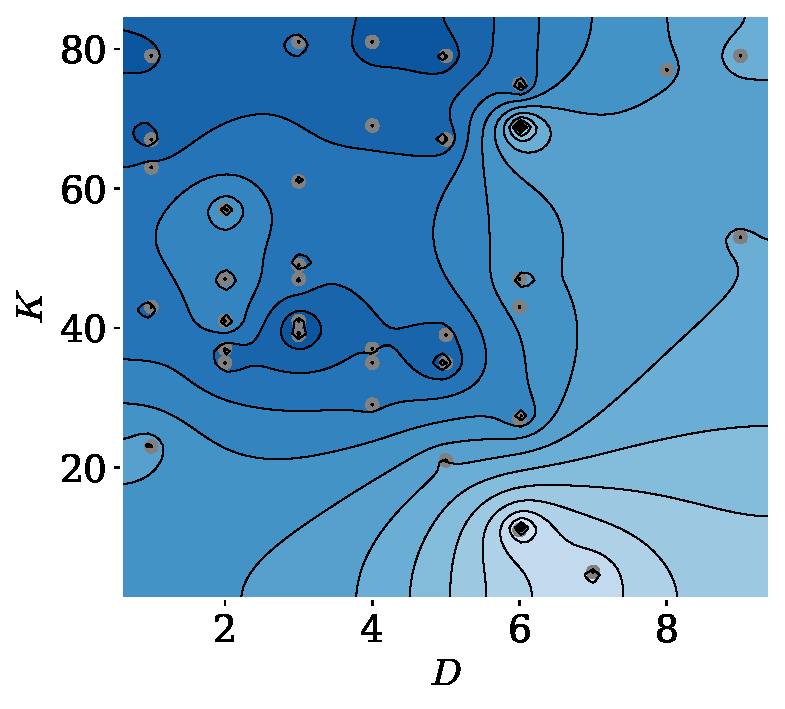
\includegraphics[width=\FW,height=\FH]{Figures/contour_D_vs_K-14.pdf}} 
\subfloat[$D'$ vs. $K$]{%
  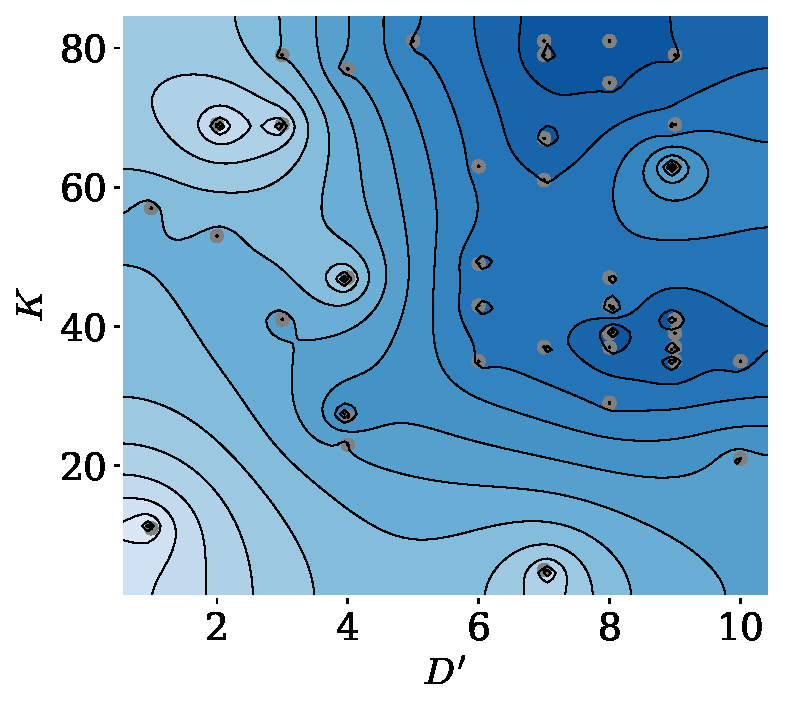
\includegraphics[width=\FW,height=\FH]{Figures/contour_Dprime_vs_K-14.pdf}} 
\subfloat[$D$vs. $\mu$]{%
  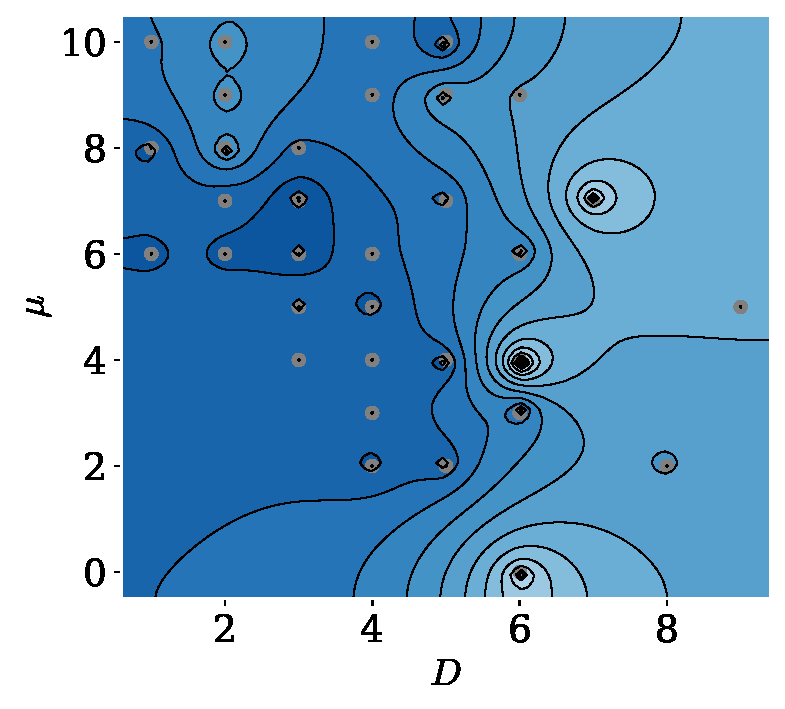
\includegraphics[width=\FW,height=\FH]{Figures/contour_D_vs_mu-14.pdf}} \\[0.6em]

% --------- FILA 2 ----------
\subfloat[$D'$ vs.$\mu$]{%
  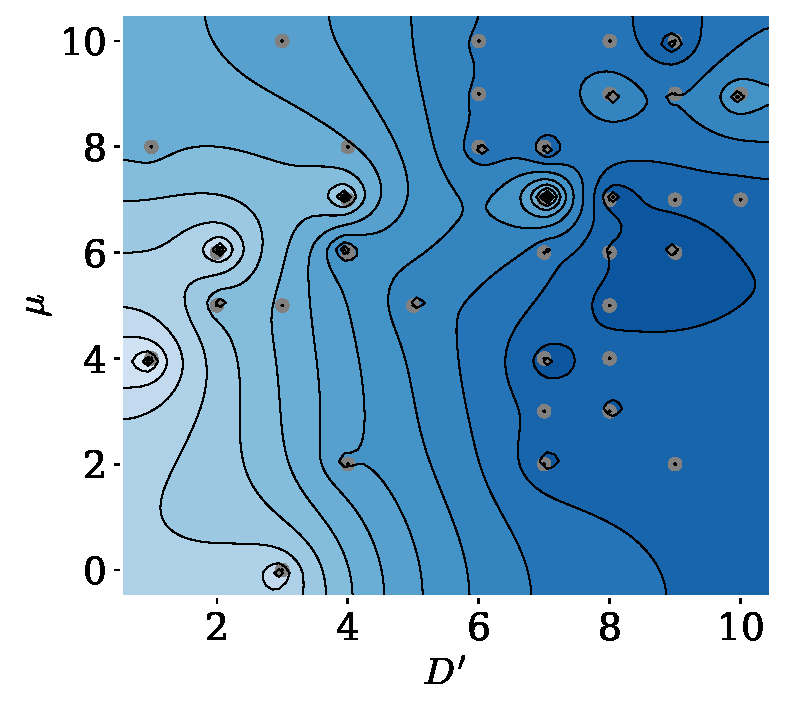
\includegraphics[width=\FW,height=\FH]{Figures/contour_Dprime_vs_mu-14.pdf}} 
\subfloat[$\tau$vs. $\mu$]{%
  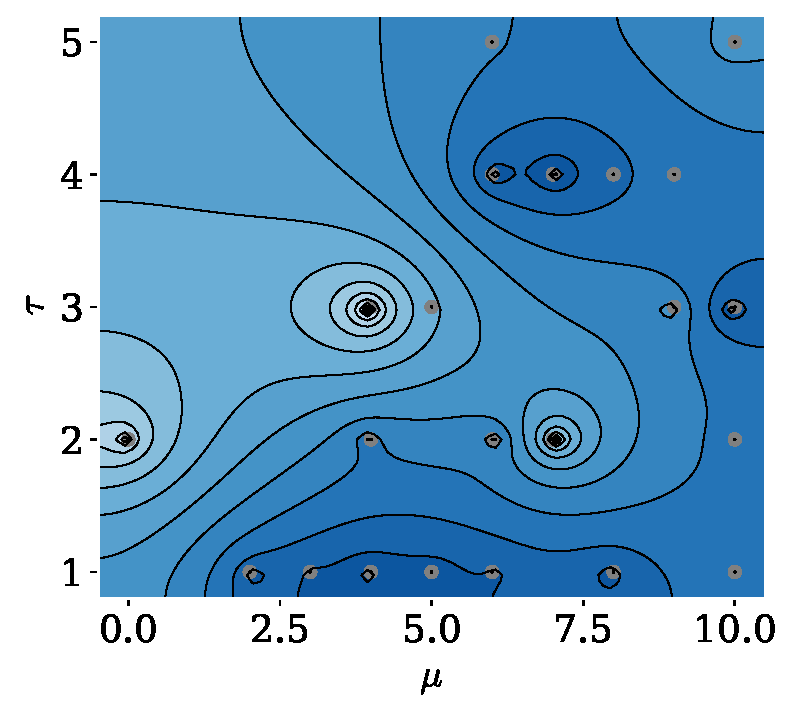
\includegraphics[width=\FW,height=\FH]{Figures/contour_mu_vs_tau-14.pdf}} 
\subfloat[$D'$ vs. $D$]{%
  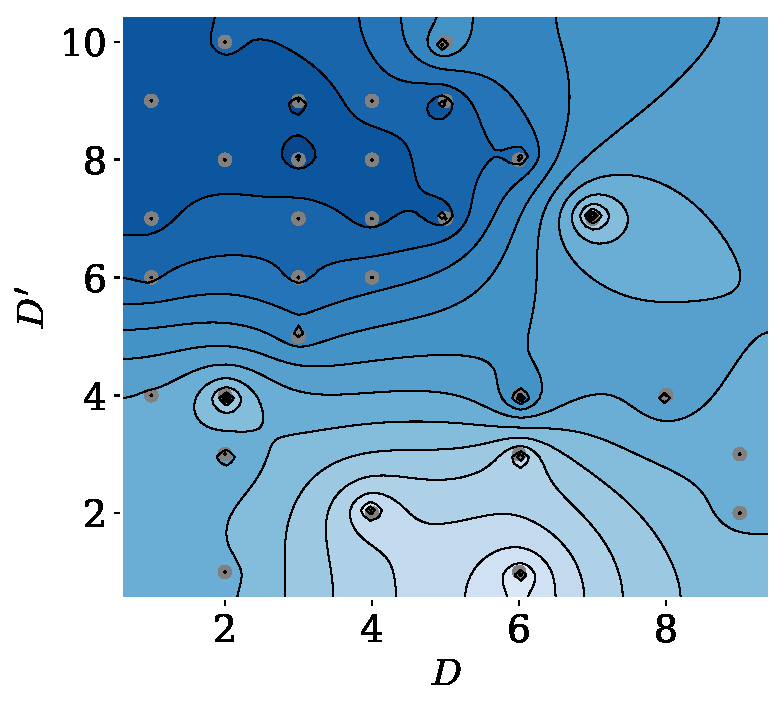
\includegraphics[width=\FW,height=\FH]{Figures/contour_D_vs_Dprime-14.pdf}} \\[0.8em]

% ================= COLORBAR HORIZONTAL (COMPARTIDO) =================
\begin{tikzpicture}
\begin{axis}[
  hide axis,
  scale only axis,
  width=\linewidth,
  height=0pt,
  colormap name=optunablues,
  colorbar horizontal,
  point meta min=60,
  point meta max=92,
  colorbar style={
    width=\linewidth,
    height=3mm,
    xtick={60, 64, 68, 72, 76, 80, 84, 88, 92},
    xticklabel style={font=\scriptsize},
    xlabel={val accuracy (\%)},
    xlabel style={font=\scriptsize, yshift=2pt},
    scaled ticks=false,
    /pgf/number format/fixed,
    /pgf/number format/precision=1,
  },
]
\addplot [draw=none] coordinates {(0,0)};
\end{axis}
\end{tikzpicture}

\end{minipage}%
}

\caption{{Contour plots of validation accuracy (\%) for \gls{tektenet} as a function of selected hyperparameter pairs for Subject~14 from the GigaScience dataset. All panels share the same color scale, allowing direct visual comparison across hyperparameter pairs within the subject.}}
\label{fig:global_freq_Giga14}
\end{figure}

%----------------------------------------------------

{In contrast, for the low-performing subject (Subject~27), the contour plots in Fig.~\ref{fig:global_freq_giga27} reveal a more constrained and fragmented optimization landscape. Compared with Subject~14, the high-performance regions are less extended and appear more localized across the explored hyperparameter space. The projections involving the temporal kernel size $K$ and the embedding dimensions ($D$, $D'$) show that favorable validation accuracy is mainly achieved within specific combinations of temporal receptive field and reconstructed state-space dimensionality, rather than across broad parameter ranges. This suggests a stronger sensitivity to the joint selection of $K$, $D$, and $D'$ for this subject.}

{A similar behavior is observed in the projections involving the delay parameter $\mu$, where favorable regions appear in localized zones depending on the values of $D$, $D'$, and $\tau$. This indicates that the estimation of delayed directed dependencies is more sensitive to the alignment among embedding order, stride, and interaction delay, which is consistent with the role of state-space reconstruction and transfer entropy in modeling nonlinear directed interactions~\cite{schreiber2000measuring,staniek2008symbolic}. The $D$--$D'$ projection also lacks a broad dominant region of high performance, showing instead several separated configurations with moderate-to-favorable accuracy. Overall, these patterns suggest that Subject~27 represents a more challenging optimization regime for \gls{tektenet}, in which decoding performance depends more critically on the precise balance among temporal filtering, state-space reconstruction, and delay-related parameters.}

%----------------------------------------------------
\begin{figure}[H]
\centering

% ---------- Tamaños ----------
\setlength{\FW}{0.34\linewidth}
\setlength{\FH}{3.4cm}

\makebox[\textwidth][c]{%

% ================= PANEL 3x2 + COLORBAR =================
\begin{minipage}[c]{0.99\textwidth}
\centering

% --------- FILA 1 ----------
\subfloat[$D$ vs. $K$]{%
  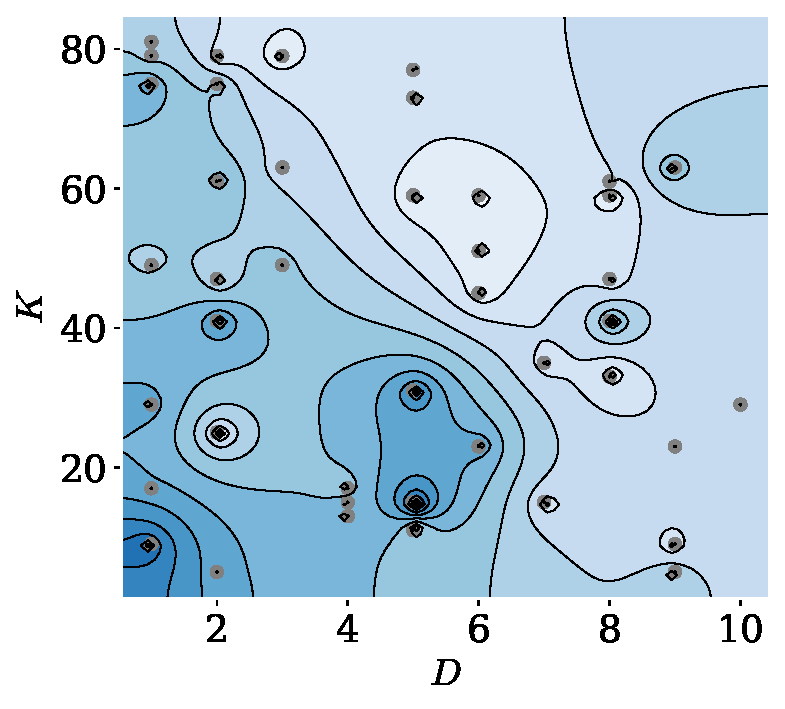
\includegraphics[width=\FW,height=\FH]{Figures/contour_D_vs_K-27.pdf}} 
\subfloat[$D'$ vs. $K$]{%
  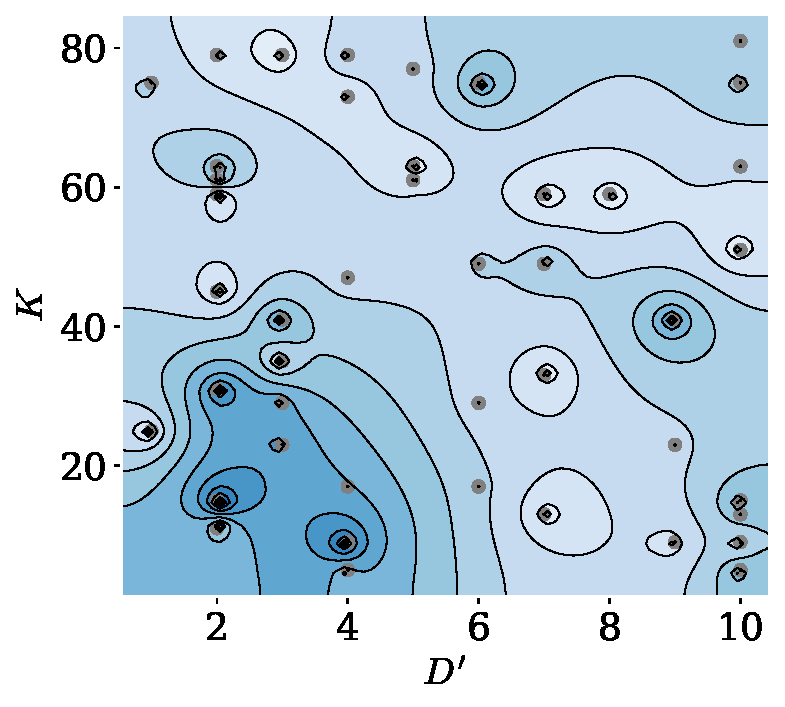
\includegraphics[width=\FW,height=\FH]{Figures/contour_Dprime_vs_K-27.pdf}} 
\subfloat[$D$ vs. $\mu$]{%
  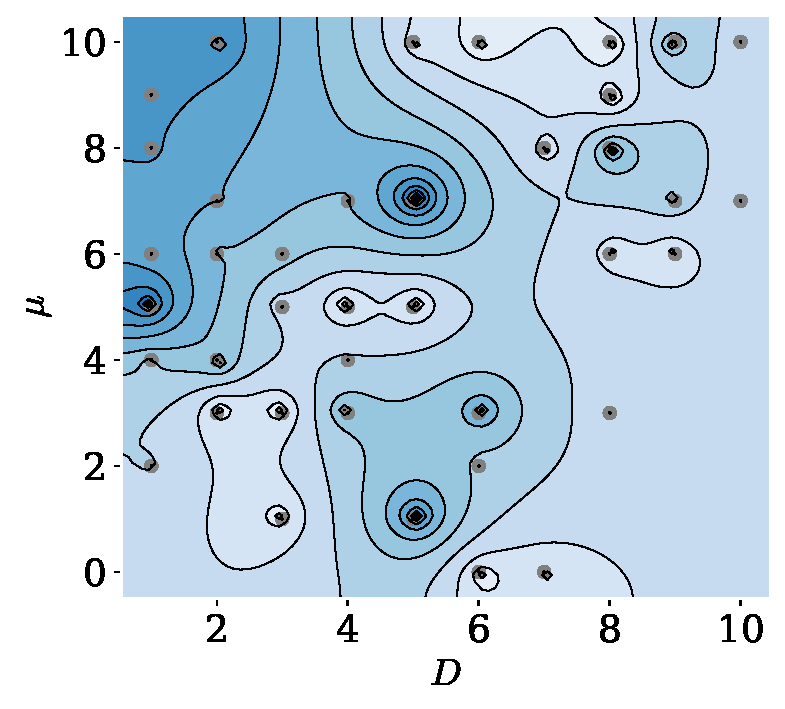
\includegraphics[width=\FW,height=\FH]{Figures/contour_D_vs_mu-27.pdf}} \\[0.6em]

% --------- FILA 2 ----------
\subfloat[$D'$ vs.$\mu$]{%
  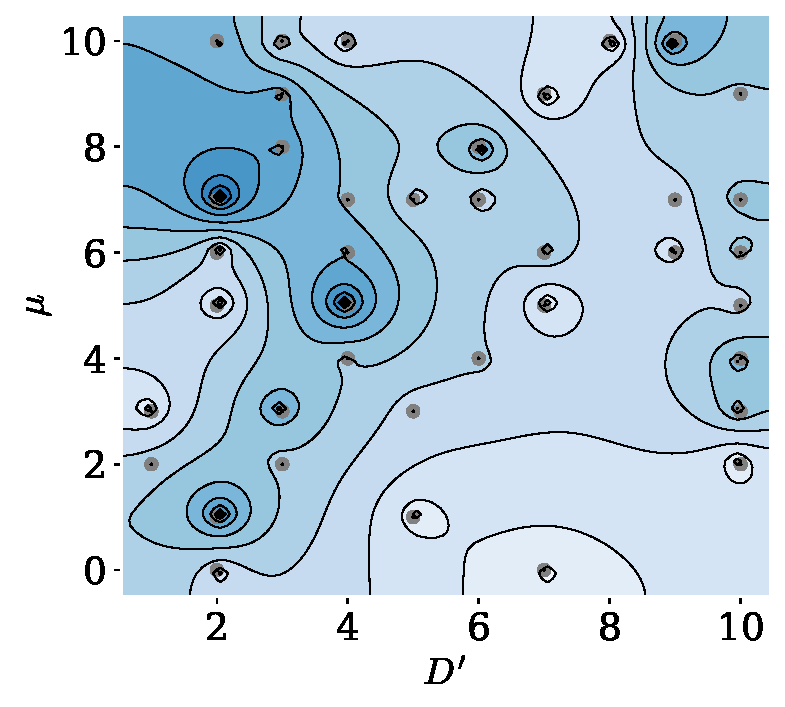
\includegraphics[width=\FW,height=\FH]{Figures/contour_Dprime_vs_mu-27.pdf}}
\subfloat[$\tau$vs. $\mu$]{%
  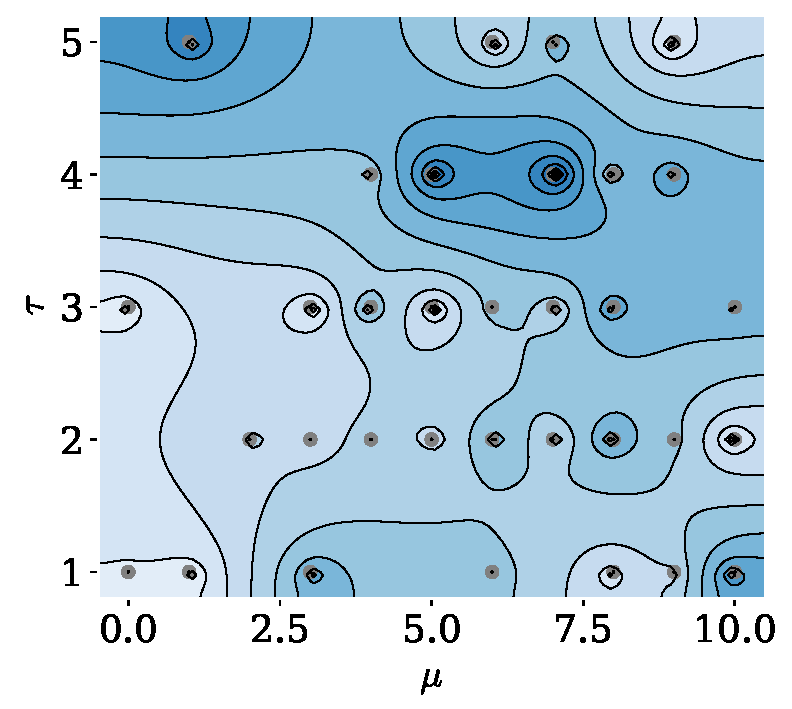
\includegraphics[width=\FW,height=\FH]{Figures/contour_mu_vs_tau-27.pdf}} 
\subfloat[$D'$ vs. $D$]{%
  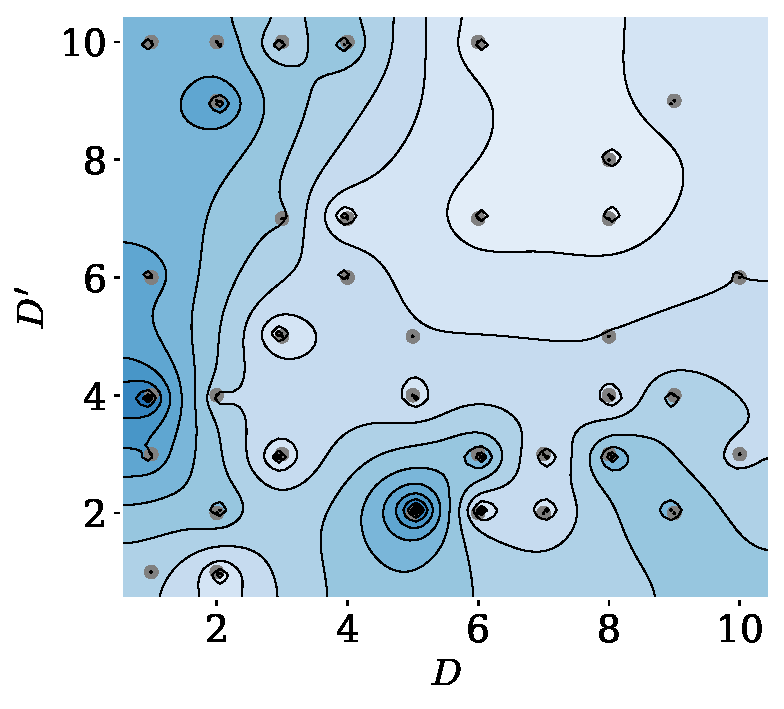
\includegraphics[width=\FW,height=\FH]{Figures/contour_D_vs_Dprime-27.pdf}} \\[0.8em]

% ================= COLORBAR HORIZONTAL (COMPARTIDO) =================
\begin{tikzpicture}
\begin{axis}[
  hide axis,
  scale only axis,
  width=\linewidth,
  height=0pt,
  colormap name=optunablues,
  colorbar horizontal,
  point meta min=51,
  point meta max=65,
  colorbar style={
    width=\linewidth,
    height=3mm,
    xtick={51, 53, 55, 57, 59, 61, 63, 65},
    xticklabel style={font=\scriptsize},
    xlabel={val accuracy (\%)},
    xlabel style={font=\scriptsize, yshift=2pt},
    scaled ticks=false,
    /pgf/number format/fixed,
    /pgf/number format/precision=1,
  },
]
\addplot [draw=none] coordinates {(0,0)};
\end{axis}
\end{tikzpicture}

\end{minipage}%
}

\caption{{Contour plots of validation accuracy (\%) for \gls{tektenet} as a function of selected hyperparameter pairs for Subject~27 from the GigaScience dataset. All panels share the same color scale, allowing direct visual comparison across hyperparameter pairs within the subject.}}
\label{fig:global_freq_giga27}
\end{figure}
%----------------------------------------------------
{To complement the subject-specific contour analysis, a global hyperparameter-importance analysis was conducted to quantify the relative contribution of each \gls{tektenet} hyperparameter to validation accuracy on the GigaScience dataset. As shown in Fig.~\ref{fig:GIGA_TE}, this analysis summarizes the influence of the temporal kernel size $K$, the stride $\tau$, the embedding orders $D$ and $D'$, and the interaction delay $\mu$ across the explored hyperparameter configurations.}

{The results show that the temporal kernel size $K$ and the stride $\tau$ are the most influential hyperparameters, with importance scores of $0.33$ and $0.31$, respectively. Together, these two parameters account for the largest proportion of the global importance, suggesting that \gls{tektenet} performance on the GigaScience dataset is mainly driven by the temporal receptive field and the stride-related sampling of the reconstructed dynamics. This result highlights the relevance of how temporal information is locally filtered and subsequently organized for Takens-based connectivity estimation~\cite{schreiber2000measuring}.}

{In contrast, the embedding order $D$ and the interaction delay $\mu$ exhibit moderate importance scores of $0.15$ and $0.14$, respectively, indicating that state-space reconstruction and delayed directed interactions also contribute to validation accuracy, although their influence is secondary compared with $K$ and $\tau$. Finally, $D'$ shows the lowest importance score ($0.07$), suggesting that, within the explored range, \gls{tektenet} is less sensitive to this embedding dimension. Overall, these findings indicate that temporal filtering and stride-related dynamics constitute the main drivers of performance, while the remaining Takens-based parameters provide complementary adjustments to the effective-connectivity representation.}
%----------------------------------------------------
\begin{figure}[H]
    \centering
    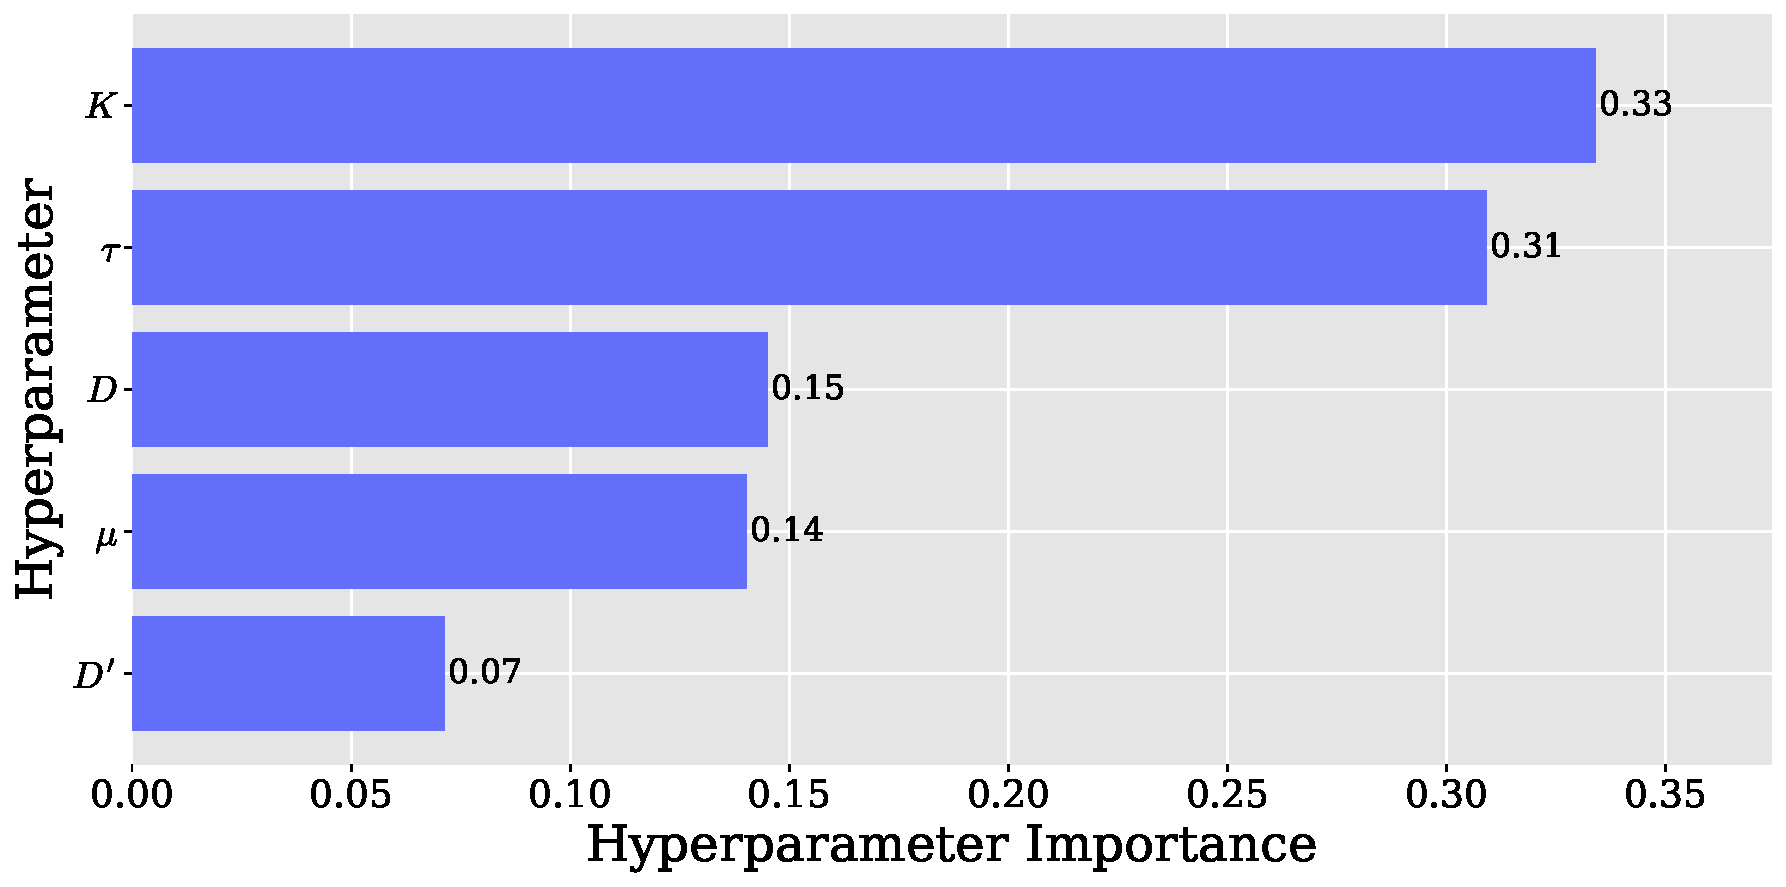
\includegraphics[width=0.8\linewidth]{Figures/optuna_fanova_param_importances_tekte-GIGA.pdf}
    \caption{{Global hyperparameter importance analysis for \gls{tektenet} on the GigaScience dataset. Importance scores quantify the relative contribution of the temporal kernel size $K$, stride $\tau$, embedding orders $D$ and $D'$, and interaction delay $\mu$ to validation accuracy.}}
    \label{fig:GIGA_TE}
\end{figure}
%----------------------------------------------------


\subsubsection{Validation on complex scenarios: Multi-class decoding on \gls{eegmmidb} collection}

To assess the scalability of the proposed framework beyond binary classification, its performance was evaluated on the \gls{eegmmidb} dataset, which poses a challenging five-class \gls{mi} decoding task. This scenario requires the model to disentangle multiple distinct neural patterns (Left Hand, Right Hand, Both Hands, Both Feet, and Rest), thereby significantly increasing the complexity of the decision boundaries compared to the binary BCI Competition IV-2a setting {evaluated within this contribution}.

Beyond the overall classification results, this experiment also enabled an analysis of the robustness and adaptability of the proposed framework under inter-subject variability by incorporating a systematic Bayesian hyperparameter optimization procedure. For each subject, the model's structural and temporal hyperparameters, namely the embedding orders $D$ and $D'$, the stride $\tau$, the interaction delay $\mu$, and the temporal kernel size $K$, were automatically tuned to maximize validation performance under a controlled evaluation protocol.

%---------------------------------------------------------------------------------
\begin{table}[htbp]
\centering
\caption{Subject-specific \gls{tektenet} hyperparameters selected through Bayesian optimization on the \gls{eegmmidb} dataset.}
\label{tab:hyperparameters_physionet}
\begin{tabular}{crrrrrr}
\toprule
\textbf{Subject} & \textbf{$D$} & \textbf{$D'$} & \textbf{$\tau$} & \textbf{$\mu$} & \textbf{$K$} & \textbf{Val. Acc. (\%)} \\
\midrule
3   & 3 & 1 & 3 & 16 & 16 & 76.19 \\
7   & 4 & 4 & 3 & 16 & 22 & 74.61 \\
8   & 1 & 1 & 4 & 13 & 32 & 77.78 \\
9   & 3 & 3 & 3 & 11 & 22 & 74.60 \\
12  & 4 & 4 & 4 & 12 & 16 & 77.77 \\
13  & 6 & 3 & 2 & 19 & 22 & 77.76 \\
40  & 5 & 1 & 5 & 18 & 22 & 74.59 \\
41  & 6 & 3 & 4 & 10 & 22 & 76.18 \\
49  & 1 & 4 & 4 & 17 & 16 & 77.75 \\
50  & 1 & 1 & 4 & 10 & 16 & 77.74 \\
\midrule
\textbf{Average} &  &  &  &  &  & \textbf{76.50} \\
\bottomrule
\end{tabular}
\end{table}
%---------------------------------------------------------------------------------
The results summarized in Table~\ref{tab:hyperparameters_physionet} show that \gls{tektenet} achieves stable validation performance across the evaluated subjects, with an average validation accuracy of $76.50\%$ in the five-class \gls{eegmmidb} scenario. Despite the increased complexity of multi-class decoding, the subject-wise validation accuracies remain within a relatively narrow range, from $74.59\%$ to $77.78\%$. This suggests that the Bayesian optimization procedure was able to identify subject-specific hyperparameter configurations that preserve consistent performance under heterogeneous \gls{eeg} conditions~\cite{snoek2012practical}.

The selected configurations also show variability across subjects, particularly in the embedding orders $D$ and $D'$, the interaction delay $\mu$, and the temporal kernel size $K$. This behavior indicates that different subjects may require different balances between state-space reconstruction, temporal filtering, and delayed directed-dependency modeling, which is consistent with the role of embedding-based reconstruction and transfer entropy in capturing nonlinear directed interactions~\cite{takens1981detecting,schreiber2000measuring}. Therefore, the results support the relevance of subject-adaptive hyperparameter tuning when scaling \gls{tektenet} from binary decoding scenarios to more complex multi-class \gls{mi} tasks.

Overall, these findings suggest that the joint integration of connectivity-driven representations and Bayesian hyperparameter optimization contributes to the scalability of \gls{tektenet} on the \gls{eegmmidb} dataset, allowing the proposed framework to adapt its temporal and embedding-related parameters while preserving stable inter-subject validation performance.

%--------------------------------------------------------
%% Contours 
%--------------------------------------------------------
{To further characterize the hyperparameter landscape in this multi-class scenario, contour plots were generated for two representative subjects from the \gls{eegmmidb} dataset: Subject~12 and Subject~41. These subjects were selected to maintain consistency with the previous EEG-GCIRNet analysis, where Subject~12 represented a high-performing case and Subject~41 corresponded to a comparatively more challenging subject in the same multi-class setting. Using the same subjects allows a coherent cross-method interpretation of how different connectivity-aware frameworks behave under favorable and difficult subject-specific conditions.}

{The plots show how validation accuracy varies across selected pairs of \gls{tektenet} hyperparameters based on the configurations evaluated during the Bayesian optimization process. Thus, the contour analysis provides a visual approximation of the explored hyperparameter performance landscape, allowing the identification of favorable regions, localized optima, and configurations in which the model becomes more sensitive to specific hyperparameter choices.}
%----------------------------------------------------------
%---------------------------------------------------------------------------------
\begin{figure}[H]
\centering

% ---------- Tamaños ----------
\setlength{\FW}{0.34\linewidth}
\setlength{\FH}{3.4cm}

\makebox[\textwidth][c]{%

% ================= PANEL 3x2 + COLORBAR =================
\begin{minipage}[c]{0.99\textwidth}
\centering

% --------- FILA 1 ----------
\subfloat[$D$ vs. $K$]{%
  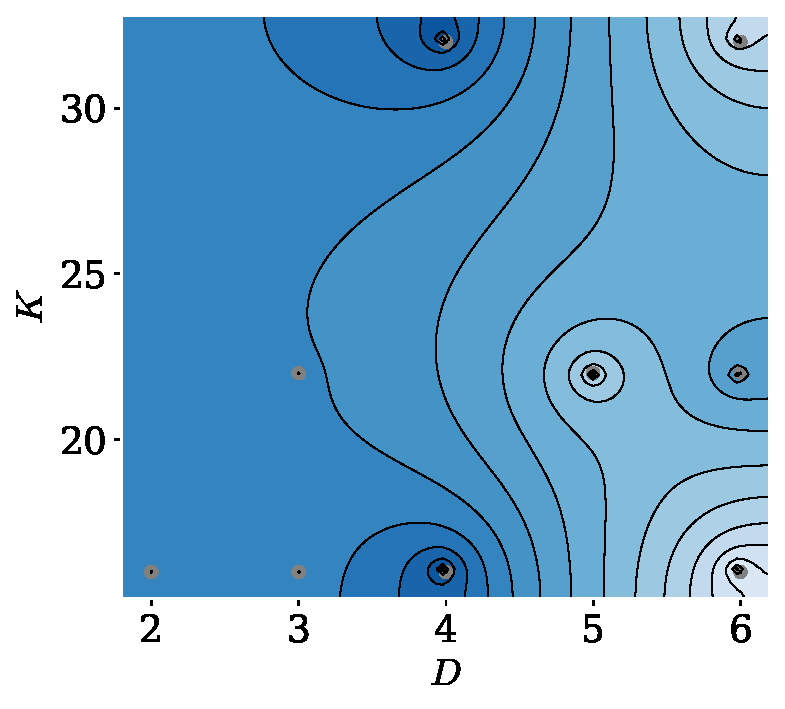
\includegraphics[width=\FW,height=\FH]{Figures/contour_D_vs_K-12.pdf}} 
\subfloat[$D'$ vs. $K$]{%
  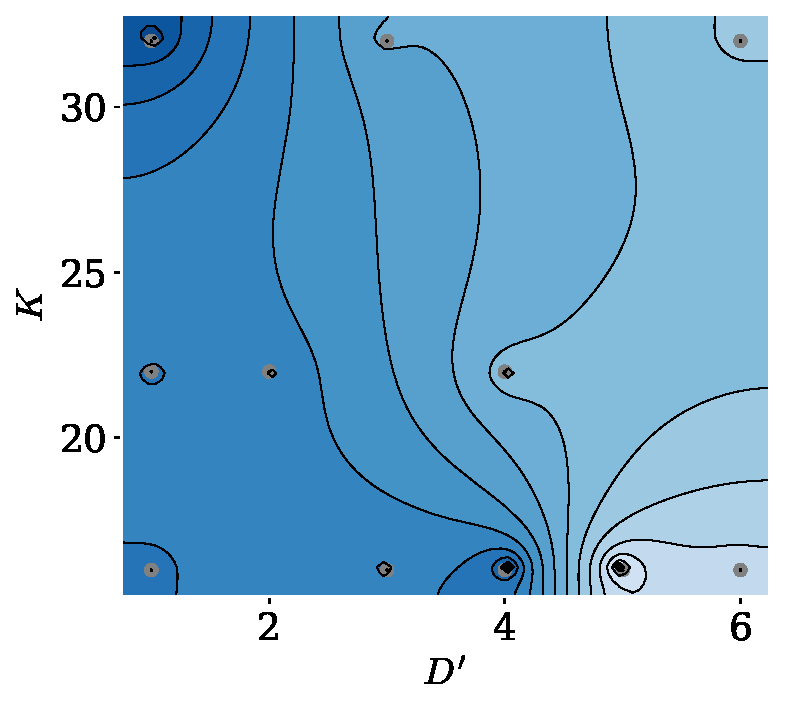
\includegraphics[width=\FW,height=\FH]{Figures/contour_Dprime_vs_K-12.pdf}} 
\subfloat[$D$vs. $\mu$]{%
  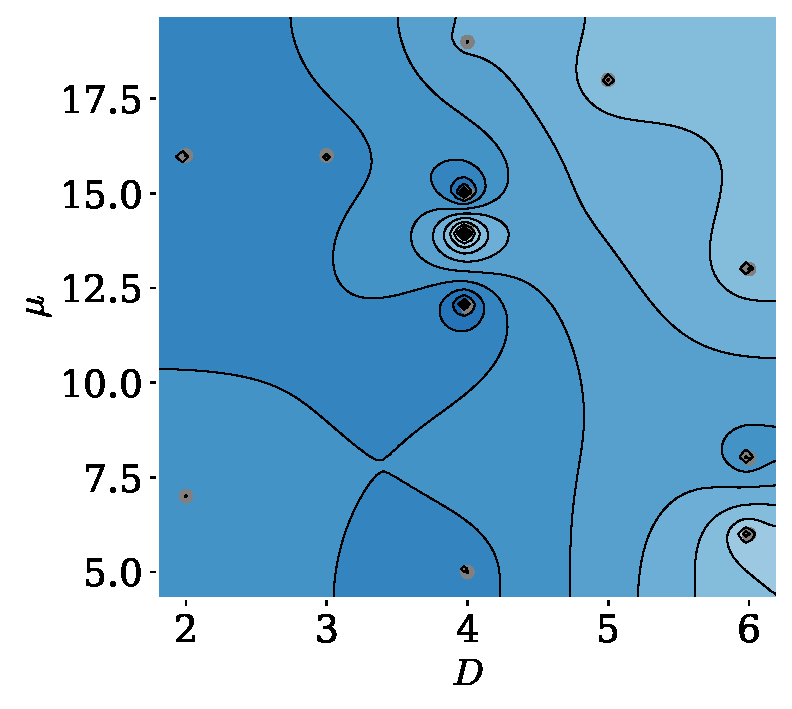
\includegraphics[width=\FW,height=\FH]{Figures/contour_D_vs_mu-12.pdf}} \\[0.6em]

% --------- FILA 2 ----------
\subfloat[$D'$ vs.$\mu$]{%
  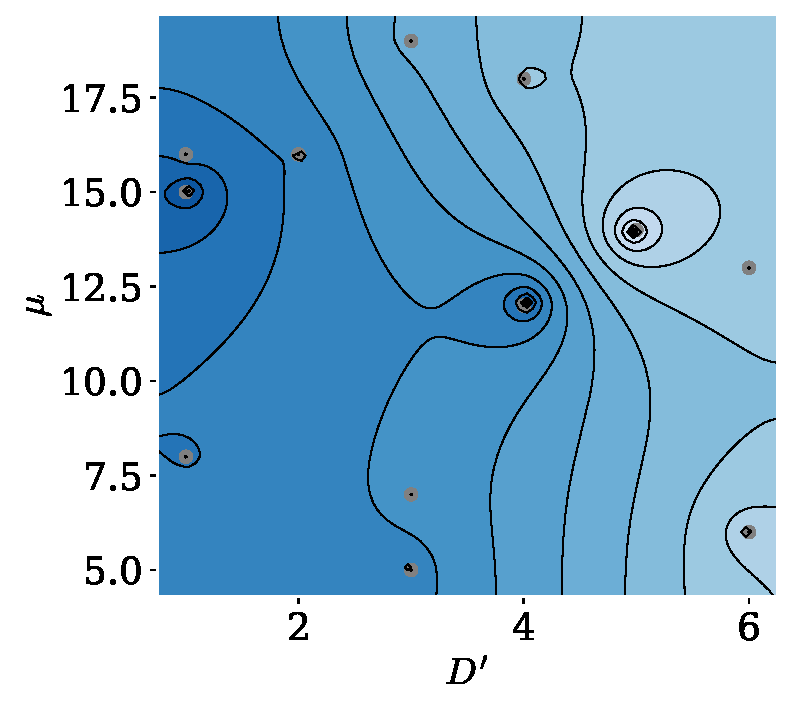
\includegraphics[width=\FW,height=\FH]{Figures/contour_Dprime_vs_mu-12.pdf}} 
\subfloat[$\tau$vs. $\mu$]{%
  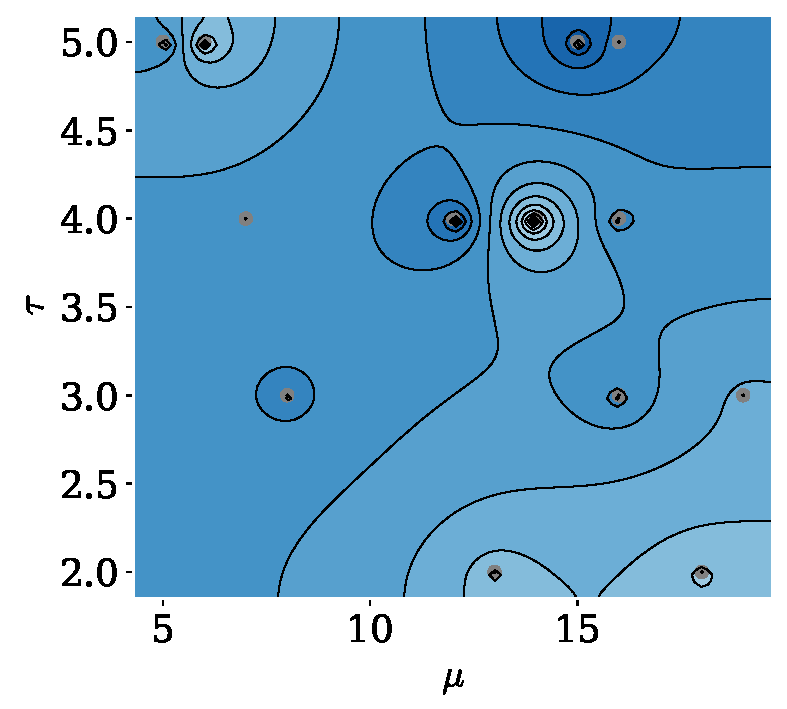
\includegraphics[width=\FW,height=\FH]{Figures/contour_mu_vs_tau-12.pdf}}
\subfloat[$D'$ vs. $D$]{%
  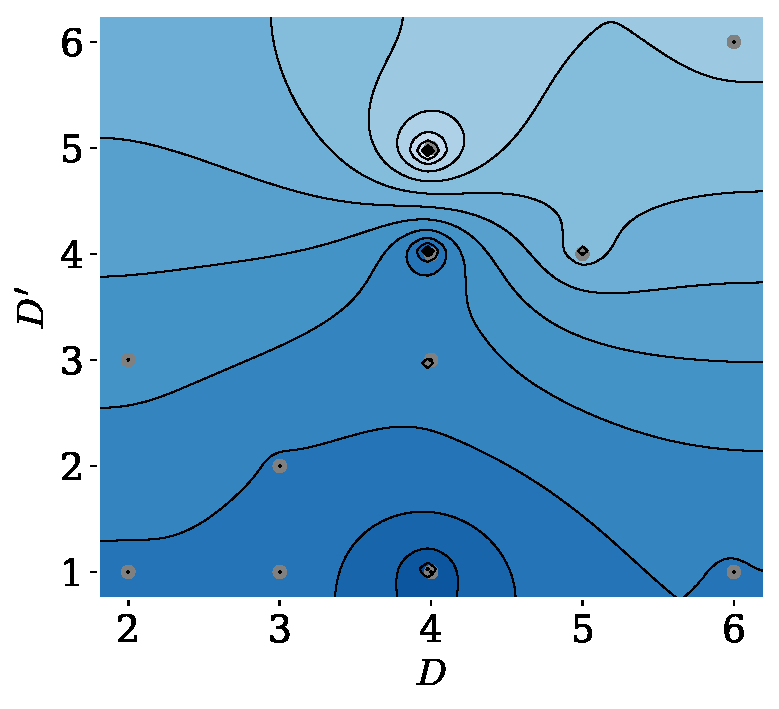
\includegraphics[width=\FW,height=\FH]{Figures/contour_D_vs_Dprime-12.pdf}} \\[0.8em]

% ================= COLORBAR HORIZONTAL (COMPARTIDO) =================
\begin{tikzpicture}
\begin{axis}[
  hide axis,
  scale only axis,
  width=\linewidth,
  height=0pt,
  colormap name=optunablues,
  colorbar horizontal,
  point meta min=64.8,
  point meta max=77.6,
  colorbar style={
    width=\linewidth,
    height=3mm,
    xtick={64.8,66.4,68.0,69.6,71.2,72.8,74.4,76.0,77.6},
    xticklabel style={font=\scriptsize},
    xlabel={val accuracy (\%)},
    xlabel style={font=\scriptsize, yshift=2pt},
    scaled ticks=false,
    /pgf/number format/fixed,
    /pgf/number format/precision=1,
  },
]
\addplot [draw=none] coordinates {(0,0)};
\end{axis}
\end{tikzpicture}

\end{minipage}%
}

\caption{{Contour plots of validation accuracy (\%) for \gls{tektenet} as a function of selected hyperparameter pairs for Subject~12 from the \gls{eegmmidb} dataset. All panels share the same color scale, allowing direct visual comparison across hyperparameter pairs within the subject.}}
\label{fig:global_freq_Phy12}
\end{figure}

%---------------------------------------------------------------------------------
{For the high-performing subject (Subject~12), the contour plots in Fig.~\ref{fig:global_freq_Phy12} reveal a relatively organized and structured optimization landscape, with well-defined high-performance regions rather than highly fragmented optima. In particular, the projections involving the temporal kernel size $K$ suggest that better validation accuracy is generally associated with larger receptive fields combined with low-to-moderate embedding orders. Likewise, the $\mu$-based projections show organized and interpretable trends, with favorable regions concentrated around intermediate values of $\mu$ and only localized performance drops for specific hyperparameter combinations. The $\mu$--$\tau$ interaction also remains relatively coherent, indicating that the alignment between interaction delay and stride is reasonably stable for this subject, which is consistent with the role of temporal embedding choices in nonlinear directed-dependency estimation~\cite{takens1981detecting, schreiber2000measuring}. Finally, the $D$--$D'$ interaction exhibits a structured surface with several competitive configurations, although jointly large embedding orders appear less favorable. Overall, these patterns suggest that, even in this more challenging multi-class setting, \gls{tektenet} operates under a relatively favorable hyperparameter regime for high-performing subjects, where performance depends on structured parameter interactions rather than on isolated sharp optima.}

%---------------------------------------------------------------------------------
\begin{figure}[H]
\centering

% ---------- Tamaños ----------
\setlength{\FW}{0.34\linewidth}
\setlength{\FH}{3.4cm}

\makebox[\textwidth][c]{%

% ================= PANEL 3x2 + COLORBAR =================
\begin{minipage}[c]{0.99\textwidth}
\centering

% --------- FILA 1 ----------
\subfloat[$D$ vs. $K$]{%
  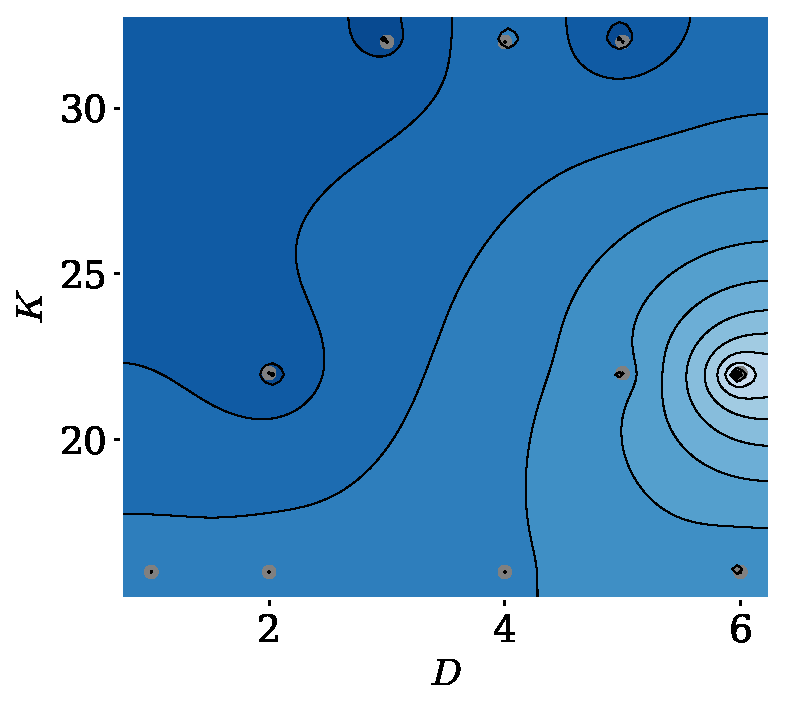
\includegraphics[width=\FW,height=\FH]{Figures/contour_D_vs_K-41.pdf}} 
\subfloat[$D'$ vs. $K$]{%
  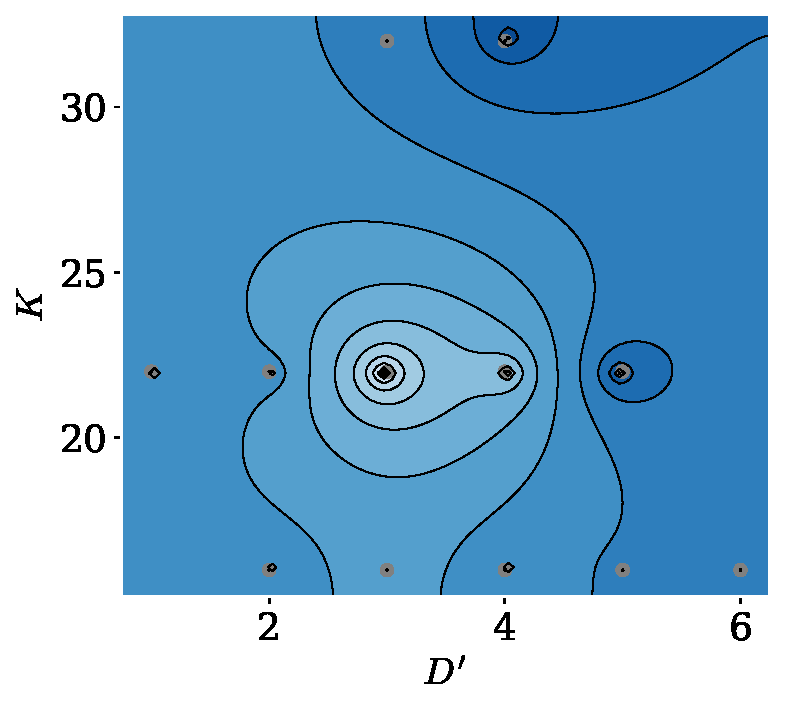
\includegraphics[width=\FW,height=\FH]{Figures/contour_Dprime_vs_K-41.pdf}} 
\subfloat[$D$vs. $\mu$]{%
  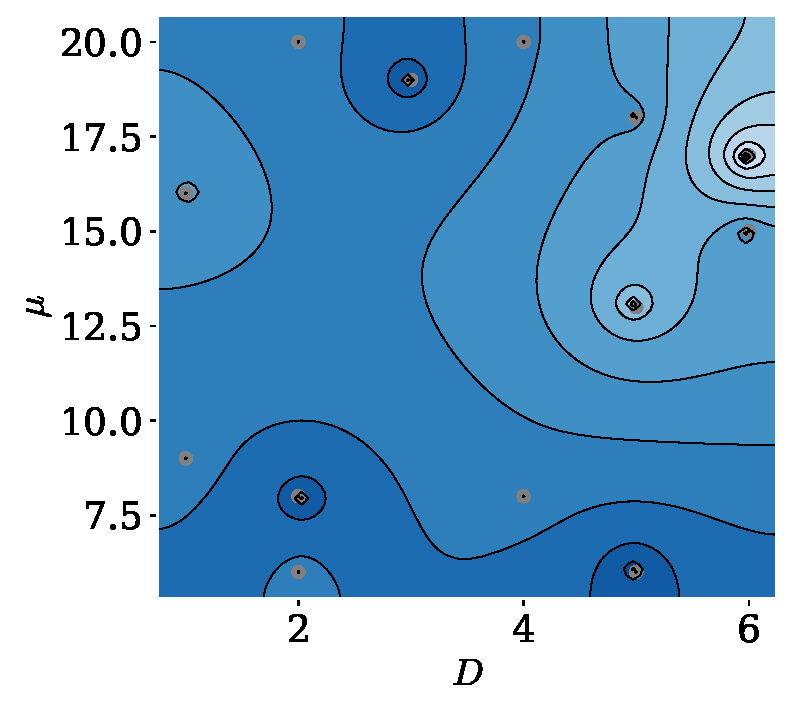
\includegraphics[width=\FW,height=\FH]{Figures/contour_D_vs_mu-41.pdf}} \\[0.6em]

% --------- FILA 2 ----------
\subfloat[$D'$ vs.$\mu$]{%
  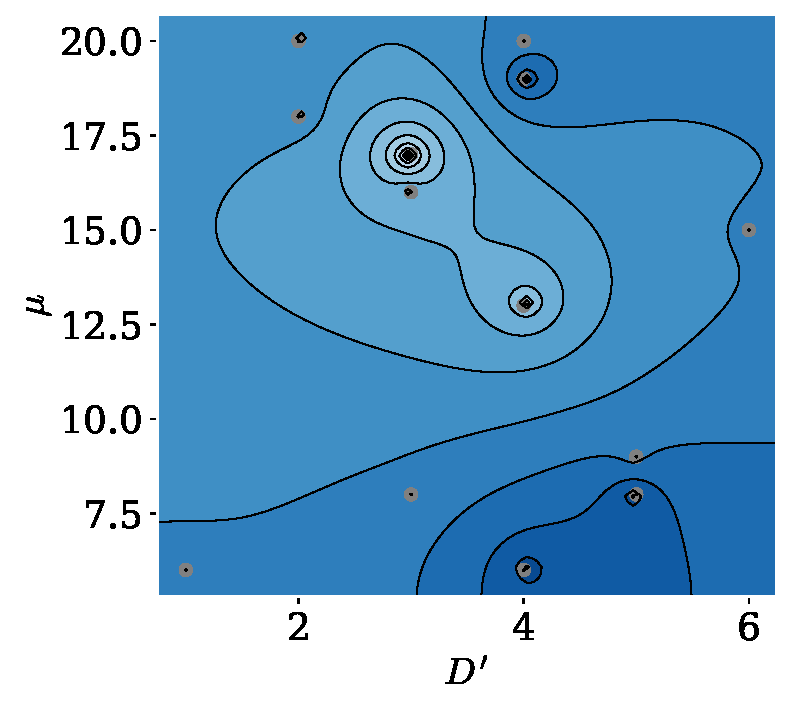
\includegraphics[width=\FW,height=\FH]{Figures/contour_Dprime_vs_mu-41.pdf}}
\subfloat[$\tau$vs. $\mu$]{%
  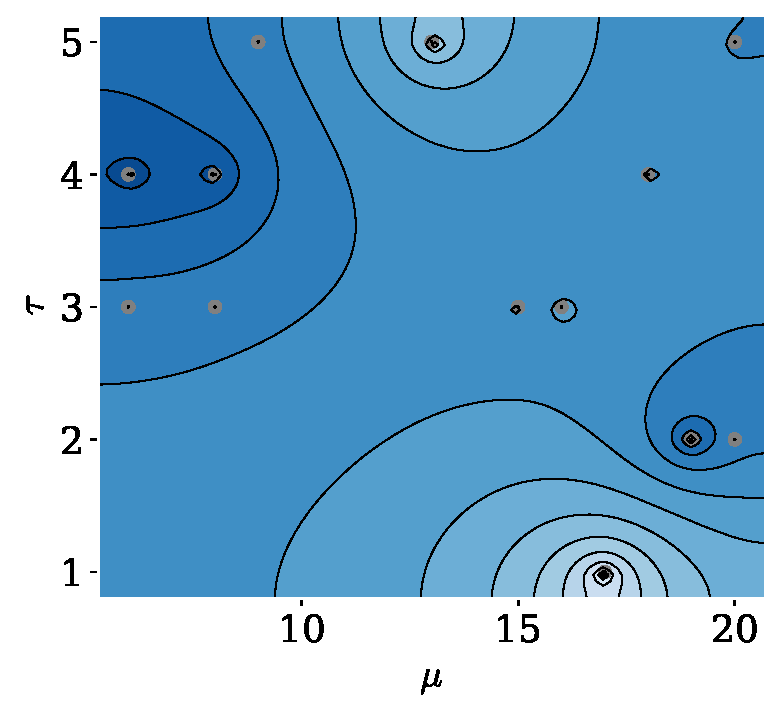
\includegraphics[width=\FW,height=\FH]{Figures/contour_mu_vs_tau-41.pdf}} 
\subfloat[$D'$ vs. $D$]{%
  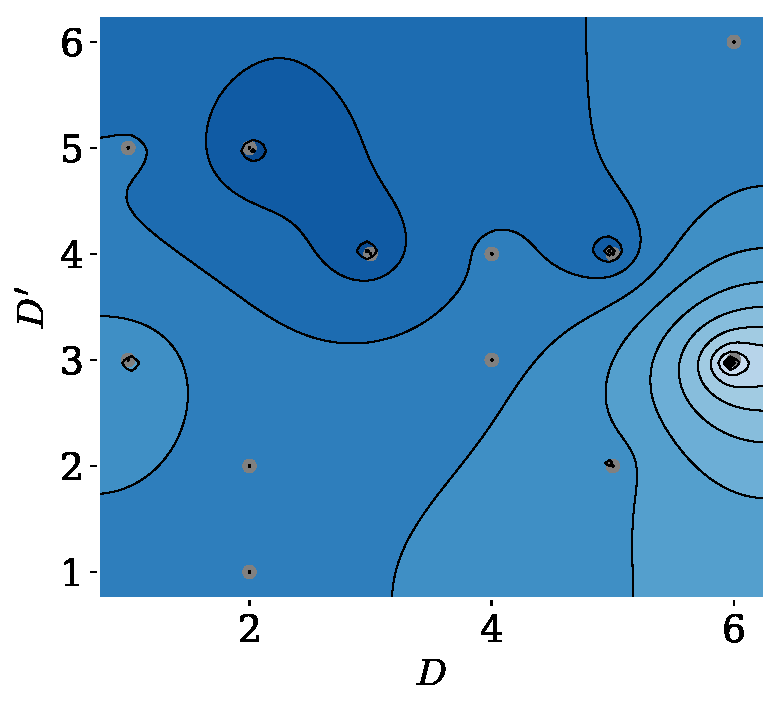
\includegraphics[width=\FW,height=\FH]{Figures/contour_D_vs_Dprime-41.pdf}} \\[0.8em]

% ================= COLORBAR HORIZONTAL (COMPARTIDO) =================
\begin{tikzpicture}
\begin{axis}[
  hide axis,
  scale only axis,
  width=\linewidth,
  height=0pt,
  colormap name=optunablues,
  colorbar horizontal,
  point meta min=64.8,
  point meta max=76.2,
  colorbar style={
    width=\linewidth,
    height=3mm,
    xtick={64.8,66.4,68.0,69.6,71.2,72.8,74.4,76.2},
    xticklabel style={font=\scriptsize},
    xlabel={val accuracy (\%)},
    xlabel style={font=\scriptsize, yshift=2pt},
    scaled ticks=false,
    /pgf/number format/fixed,
    /pgf/number format/precision=1,
  },
]
\addplot [draw=none] coordinates {(0,0)};
\end{axis}
\end{tikzpicture}

\end{minipage}%
}

\caption{{Contour plots of validation accuracy (\%) for \gls{tektenet} as a function of selected hyperparameter pairs for Subject~41 from the \gls{eegmmidb} dataset. The shared color scale enables direct comparison across hyperparameter interactions within this subject.}}
\label{fig:global_freq_Phy41}
\end{figure}
%----------------------------------------------------
{In contrast, for Subject~41, the contour plots in Fig.~\ref{fig:global_freq_Phy41} reveal a less homogeneous and more subject-sensitive optimization landscape, with favorable regions interrupted by localized performance drops. In the projections involving the temporal kernel size $K$, performance appears more sensitive to its interaction with the embedding orders, particularly around intermediate regions where narrower low-performance valleys emerge. A similar behavior is observed in the $\mu$-based projections, which show stronger fluctuations and less uniformly structured favorable regions than those observed for Subject~12.}

{The $\mu$--$\tau$ interaction is especially indicative of this behavior, with more pronounced transitions between favorable and less favorable zones. This suggests that the alignment between interaction delay and stride must be more carefully adjusted for this subject, which is consistent with the role of temporal embedding choices in nonlinear directed-dependency estimation~\cite{takens1981detecting, schreiber2000measuring}. The $D$--$D'$ interaction also lacks a single broad dominant regime, instead exhibiting multiple localized configurations with comparable performance. Overall, these patterns suggest that, in this multi-class setting, \gls{tektenet} operates under a sharper and more subject-sensitive hyperparameter regime for comparatively more challenging subjects, where performance depends more critically on the coordination among temporal filtering, state-space reconstruction, and delay-related parameters.}

{To complement the subject-specific contour analysis, a global hyperparameter-importance analysis was conducted to quantify the relative contribution of each \gls{tektenet} hyperparameter to validation accuracy on the \gls{eegmmidb} dataset. As shown in Fig.~\ref{fig:PHYSIONET_TE}, this analysis summarizes the influence of the embedding orders $D$ and $D'$, the interaction delay $\mu$, the stride $\tau$, and the temporal kernel size $K$ across the explored hyperparameter configurations.}

{The results show that the embedding orders $D'$ and $D$ are the most influential hyperparameters, with importance scores of $0.40$ and $0.27$, respectively. Together, these parameters account for the largest proportion of the global importance, suggesting that \gls{tektenet} performance on the \gls{eegmmidb} dataset is mainly driven by the configuration of the reconstructed state-space representation. This result indicates that, in the five-class decoding scenario, the ability to organize temporal information through suitable embedding orders plays a central role in separating multiple motor-imagery-related neural patterns.}

{The interaction delay $\mu$ also exhibits a relevant contribution, with an importance score of $0.19$, indicating that delayed directed dependencies remain important for modeling nonlinear temporal interactions across \gls{eeg} channels. This behavior is consistent with the role of state-space reconstruction and transfer entropy in capturing nonlinear directed interactions between time series~\cite{takens1981detecting, schreiber2000measuring}. In contrast, the stride $\tau$ and the temporal kernel size $K$ show lower importance scores of $0.09$ and $0.05$, respectively, suggesting that, within the explored range, \gls{tektenet} is less sensitive to temporal sampling and local temporal filtering than to the embedding-related parameters. Overall, these findings indicate that \gls{tektenet} performance on the \gls{eegmmidb} dataset is primarily governed by the structure of the reconstructed embedding space, while delay-related and temporal-filtering parameters provide complementary adjustments to the effective-connectivity representation.}

%----------------------------------------------------
\begin{figure}[H]
    \centering
    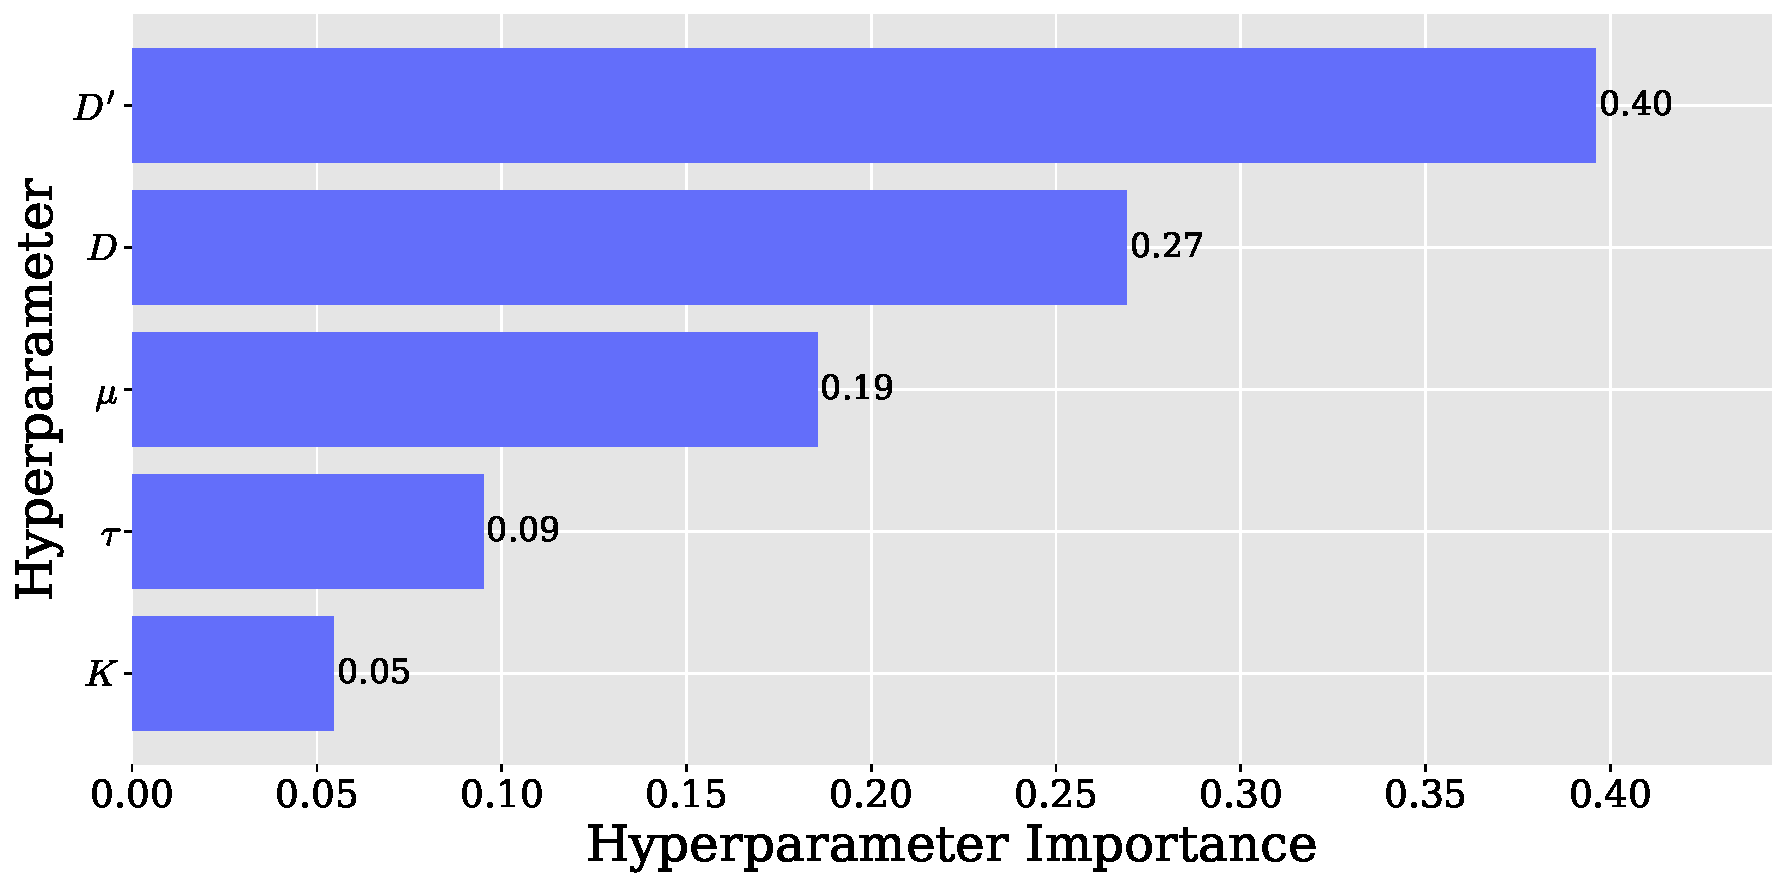
\includegraphics[width=0.8\linewidth]{Figures/optuna_fanova_param_importances_tekte-PHYSIONET.pdf}
    \caption{{Global hyperparameter importance analysis for \gls{tektenet} on the \gls{eegmmidb} dataset. Importance scores quantify the relative contribution of the embedding orders $D$ and $D'$, interaction delay $\mu$, stride $\tau$, and temporal kernel size $K$ to validation accuracy.}}
    \label{fig:PHYSIONET_TE}
\end{figure}
%----------------------------------------------------
\subsubsection{Subject-Group Validation on \gls{adhd}/control children Following SGKF-CV Protocol}

To further evaluate the generalization capability of the proposed framework under realistic and heterogeneous conditions, experiments were conducted on the \gls{adhd}/control children dataset using a Stratified Group k-Fold Cross-Validation (SGKF-CV) protocol. This validation strategy enforces subject-group separation across folds, reducing the risk of information leakage and providing a more realistic estimate of subject-independent generalization~\cite{saha2020intra}. Compared with controlled \gls{mi} benchmarks, the \gls{adhd}/control children dataset represents a more challenging scenario due to pronounced inter-subject variability, heterogeneous neurodevelopmental profiles, and less structured task-related neural patterns~\cite{lenartowicz2018adhd}.

Bayesian hyperparameter optimization identified a compact yet expressive \gls{tektenet} configuration, defined by embedding orders $D=4$ and $D'=3$, stride $\tau=1$, interaction delay $\mu=4$, and temporal kernel size $K=40$. This configuration suggests that, for the \gls{adhd}/control children dataset, discriminative information is mainly supported by short stride-based temporal sampling and moderate interaction-delay modeling, while broader temporal dependencies are captured through a relatively large temporal kernel. The best validation accuracy achieved during the optimization process was $69.95\%$, indicating that the proposed framework can extract meaningful discriminative representations even under group-based validation constraints~\cite{snoek2012practical}.

\begin{table}[H]
\centering
\caption{Fold-wise performance of \gls{tektenet} on the \gls{adhd}/control children dataset under the SGKF-CV protocol.}
\label{tab:tdha_folds}
\begin{tabular}{ccccc}
\toprule
\textbf{Fold} & \textbf{Accuracy (\%)} & \textbf{F1-score (\%)} & \textbf{Sensitivity (\%)} & \textbf{Specificity (\%)} \\
\midrule
1 & 56.64 & 63.44 & 64.85 & 45.30 \\
2 & 62.39 & 71.63 & 73.46 & 42.18 \\
3 & 61.58 & 64.12 & 69.61 & 53.78 \\
4 & 65.31 & 70.81 & 78.69 & 49.93 \\
5 & 51.60 & 56.07 & 57.89 & 44.40 \\
\midrule
\textbf{Average} & \textbf{59.50} & \textbf{65.21} & \textbf{68.90} & \textbf{47.12} \\
\bottomrule
\end{tabular}
\end{table}

Performance across the five SGKF-CV folds, reported in Table~\ref{tab:tdha_folds}, reveals moderate but meaningful generalization behavior under subject-group validation. Classification accuracy ranges from $51.60\%$ to $65.31\%$, with corresponding F1-scores between $56.07\%$ and $71.63\%$, indicating that the model retains discriminative capacity despite the strong inter-subject variability of the dataset. Notably, folds achieving higher accuracy also exhibit increased sensitivity, reaching up to $78.69\%$, suggesting that the model is able to capture neural patterns associated with the positive class for certain subject groups.

In contrast, specificity remains comparatively lower and more variable, with an average value of $47.12\%$. This behavior indicates that the model has greater difficulty correctly identifying the negative class under the SGKF-CV setting, which is consistent with the challenging nature of \gls{adhd}/control discrimination using heterogeneous pediatric \gls{eeg} recordings. The difference between sensitivity and specificity also suggests a tendency toward higher detection of the positive class, at the expense of increased confusion in the control group.

The observed inter-fold variability is consistent with the heterogeneous nature of the \gls{adhd}/control children dataset and reinforces the importance of subject-group validation protocols when assessing real-world applicability~\cite{saha2020intra}. Although the absolute performance metrics are lower than those obtained on more controlled \gls{mi} datasets, the results demonstrate that the proposed connectivity-driven representation retains meaningful discriminative power under adverse conditions. Overall, these findings suggest that the integration of nonlinear connectivity modeling, temporal encoding, and Bayesian hyperparameter optimization enables \gls{tektenet} to be extended to complex neurodevelopmental \gls{eeg} decoding scenarios, while preserving a moderate level of inter-subject generalization~\cite{schreiber2000measuring}.

{To further interpret the hyperparameter behavior under SGKF-CV, contour plots were generated from the evaluated configurations obtained during Bayesian optimization. These plots provide a global view of how validation accuracy varies across selected pairs of \gls{tektenet} hyperparameters. In contrast to the subject-wise analyses presented for the \gls{mi} datasets, these surfaces reflect the aggregated optimization behavior induced by group-based validation, where inter-fold and inter-subject variability jointly shape the hyperparameter--performance landscape.}

{Overall, the contour plots in Fig.~\ref{fig:global_freq_tdha} reveal a moderately structured but heterogeneous optimization landscape under the SGKF-CV protocol. The projections involving the temporal kernel size $K$ suggest that better validation accuracy is generally associated with moderate-to-relatively large receptive fields, particularly when combined with low-to-moderate embedding orders. This behavior is consistent with the selected configuration ($D=4$, $D'=3$, $K=40$), indicating that the model benefits from a sufficiently broad temporal kernel without relying on the largest explored values of $K$.}

{Likewise, the $\mu$-based projections indicate that favorable regions tend to appear around small-to-intermediate interaction-delay values, although with localized performance variations across embedding configurations. The $\mu$--$\tau$ interaction further suggests that compact stride-based temporal encoding, particularly with low values of $\tau$, can support favorable validation performance when paired with an appropriate interaction delay. This behavior is consistent with the role of temporal embedding choices in nonlinear directed-dependency estimation~\cite{takens1981detecting,schreiber2000measuring}. Finally, the $D$--$D'$ interaction suggests that competitive solutions are concentrated in moderate embedding-order regimes rather than at the largest explored values. Altogether, these patterns indicate that, even under the more challenging subject-group validation setting, \gls{tektenet} operates within a coherent but heterogeneous hyperparameter region characterized by compact-to-moderate embeddings, short stride-based temporal encoding, moderate interaction-delay modeling, and relatively broad temporal kernel support.}

%----------------------------------------------------
\begin{figure}[H]
\centering

% ---------- Tamaños ----------
\setlength{\FW}{0.34\linewidth}
\setlength{\FH}{3.4cm}

\makebox[\textwidth][c]{%

% ================= PANEL 3x2 + COLORBAR =================
\begin{minipage}[c]{0.99\textwidth}
\centering

% --------- FILA 1 ----------
\subfloat[$D$ vs. $K$]{%
  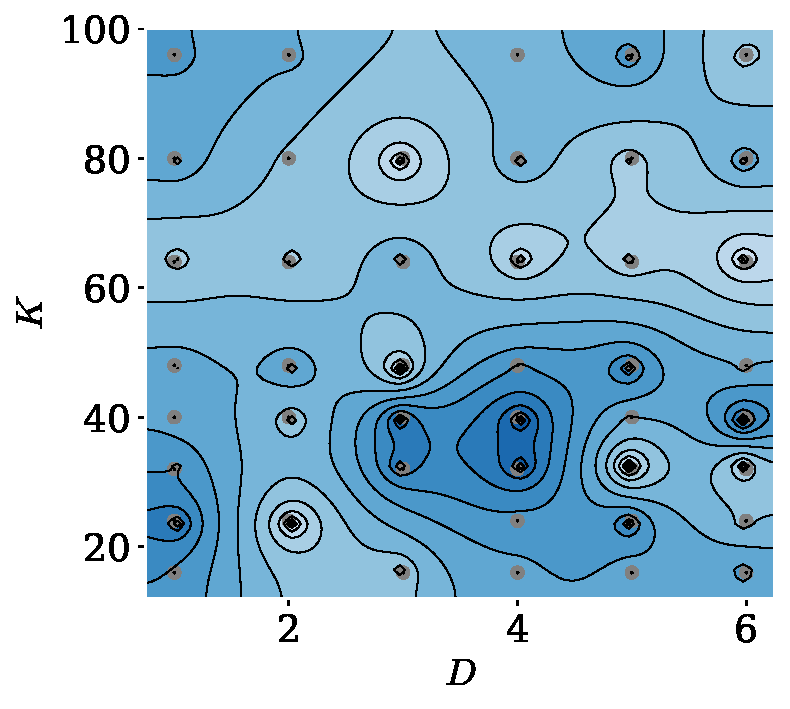
\includegraphics[width=\FW,height=\FH]{Figures/contour_D_vs_K-TDHA.pdf}}
\subfloat[$D'$ vs. $K$]{%
  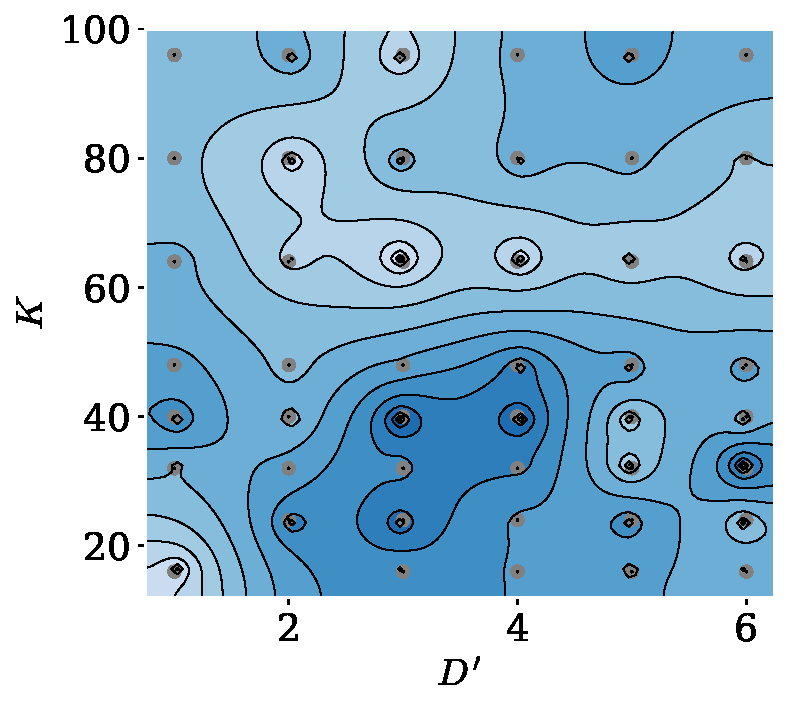
\includegraphics[width=\FW,height=\FH]{Figures/contour_Dprime_vs_K-TDHA.pdf}} 
\subfloat[$D$vs. $\mu$]{%
  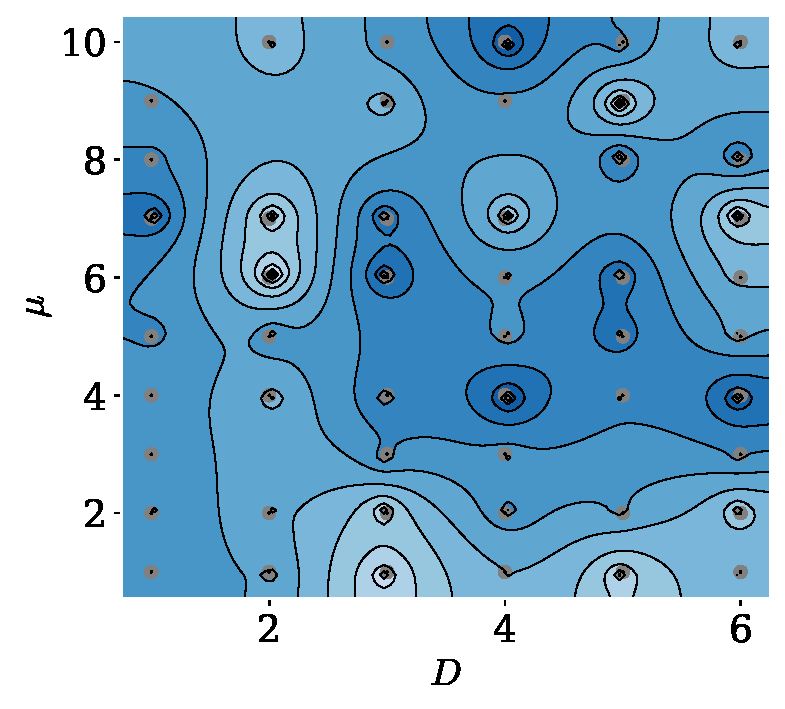
\includegraphics[width=\FW,height=\FH]{Figures/contour_D_vs_mu-TDHA.pdf}} \\[0.6em]

% --------- FILA 2 ----------
\subfloat[$D'$ vs.$\mu$]{%
  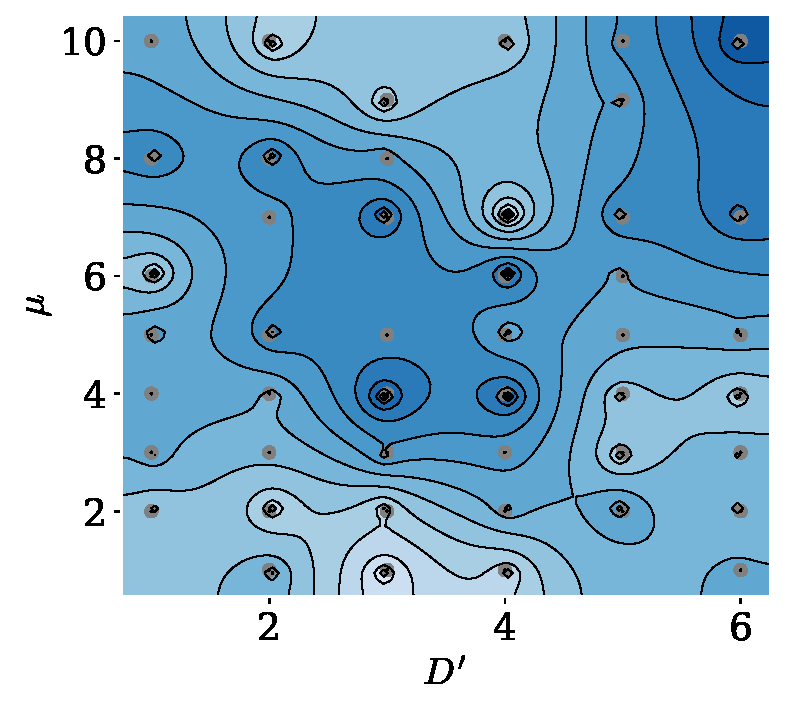
\includegraphics[width=\FW,height=\FH]{Figures/contour_Dprime_vs_mu-TDHA.pdf}} 
\subfloat[$\tau$vs. $\mu$]{%
  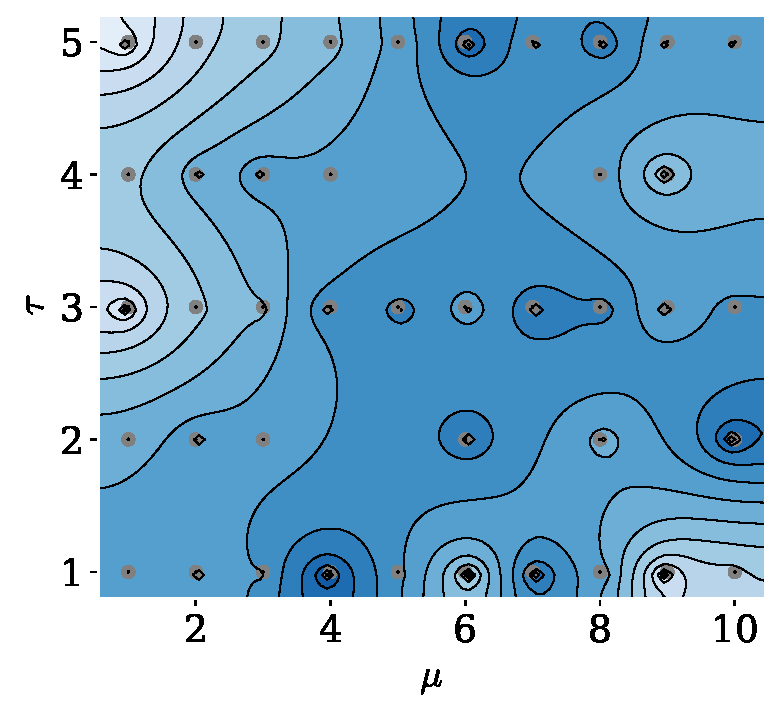
\includegraphics[width=\FW,height=\FH]{Figures/contour_mu_vs_tau-TDHA.pdf}} 
\subfloat[$D'$ vs. $D$]{%
  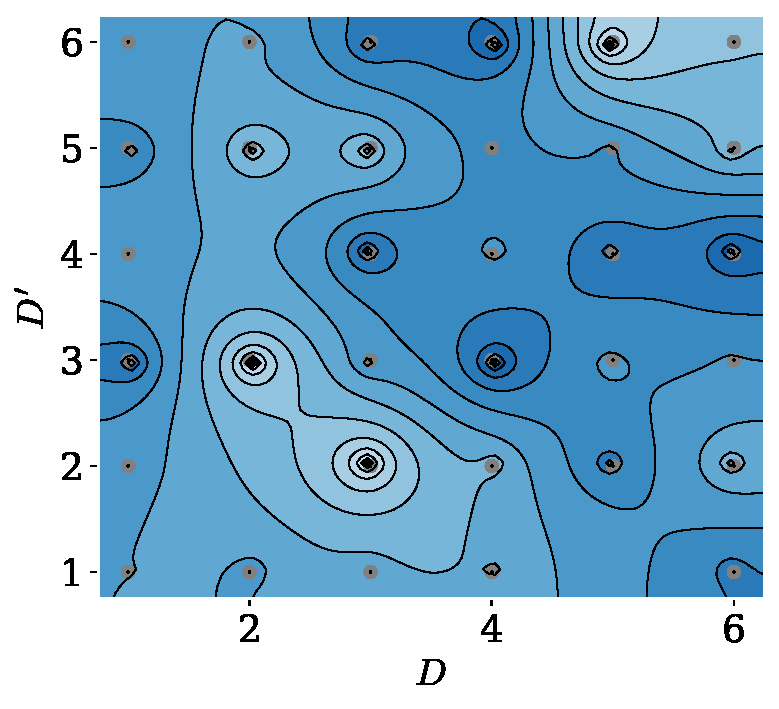
\includegraphics[width=\FW,height=\FH]{Figures/contour_D_vs_Dprime-TDHA.pdf}} \\[0.8em]

% ================= COLORBAR HORIZONTAL (COMPARTIDO) =================
\begin{tikzpicture}
\begin{axis}[
  hide axis,
  scale only axis,
  width=\linewidth,
  height=0pt,
  colormap name=optunablues,
  colorbar horizontal,
  point meta min=57.6,
  point meta max=70.4,
  colorbar style={
    width=\linewidth,
    height=3mm,
    xtick={57.6, 59.2, 60.8, 62.4, 64.0, 65.6, 67.2, 68.8, 70.4},
    xticklabel style={font=\scriptsize},
    xlabel={val accuracy (\%)},
    xlabel style={font=\scriptsize, yshift=2pt},
    scaled ticks=false,
    /pgf/number format/fixed,
    /pgf/number format/precision=1,
  },
]
\addplot [draw=none] coordinates {(0,0)};
\end{axis}
\end{tikzpicture}

\end{minipage}%
}

\caption{{Contour plots of validation accuracy (\%) for \gls{tektenet} as a function of selected hyperparameter pairs under SGKF-CV on the \gls{adhd}/control children dataset. The shared color scale enables direct comparison across hyperparameter interactions within the group-based validation setting.}}
\label{fig:global_freq_tdha}
\end{figure}
%----------------------------------------------------

{To complement the SGKF-CV contour analysis, a global hyperparameter-importance analysis was conducted to quantify the relative contribution of each \gls{tektenet} hyperparameter to validation accuracy on the \gls{adhd}/control children dataset. As shown in Fig.~\ref{fig:TDHA_TE}, this analysis summarizes the influence of the temporal kernel size $K$, the stride $\tau$, the embedding orders $D$ and $D'$, and the interaction delay $\mu$ across the explored hyperparameter configurations, following a functional analysis of variance-based importance estimation strategy~\cite{hutter2014efficient}.}

{The results show that the temporal kernel size $K$ is the most influential hyperparameter, with an importance score of $0.40$, followed by the stride $\tau$ with an importance score of $0.26$. Together, these two parameters account for the largest proportion of the global importance, suggesting that \gls{tektenet} performance on the \gls{adhd}/control children dataset is mainly driven by temporal filtering and stride-related dynamics. This result indicates that, under SGKF-CV, the model depends strongly on how local temporal information is extracted and organized before estimating nonlinear directed interactions.}

{In contrast, the embedding orders $D$ and $D'$ show lower and similar importance scores of $0.12$ and $0.11$, respectively, while the interaction delay $\mu$ also exhibits an importance score of $0.11$. This suggests that state-space reconstruction and delayed directed-dependency modeling still contribute to the validation accuracy, but their influence is secondary compared with the temporal kernel and stride parameters. Overall, these findings indicate that, in the \gls{adhd}/control children dataset, \gls{tektenet} is primarily governed by temporal filtering and compact stride-based temporal encoding, whereas the remaining Takens-based parameters provide complementary adjustments to the effective-connectivity representation~\cite{takens1981detecting,schreiber2000measuring}.}

%------------------------------------------------
\begin{figure}[H]
    \centering
    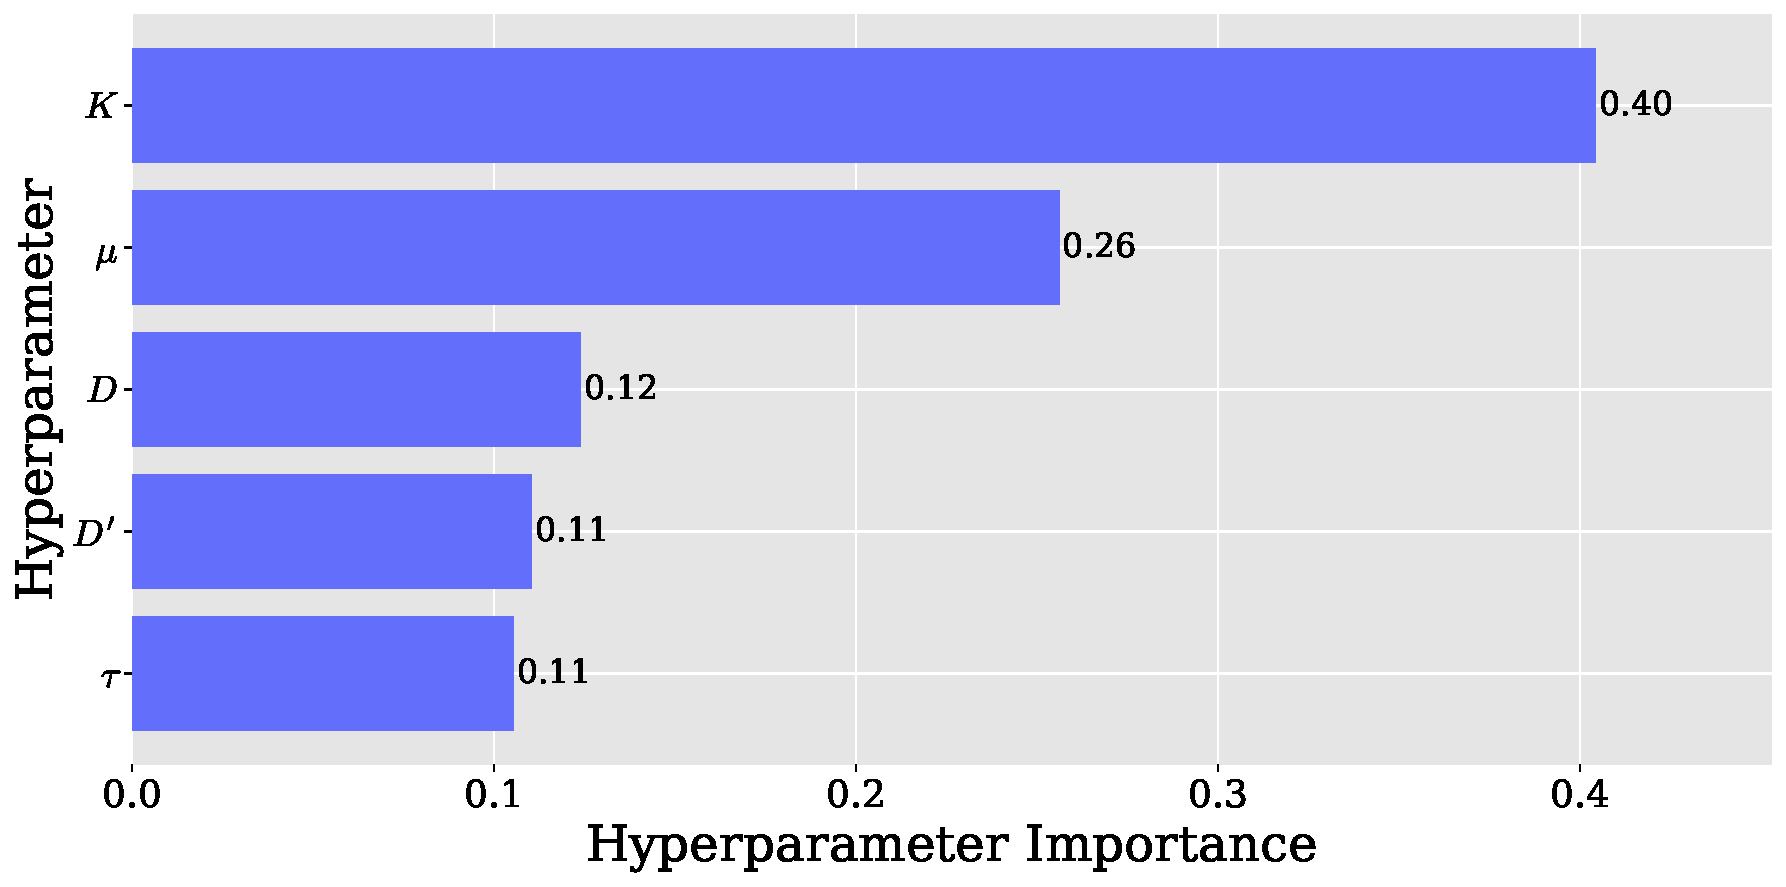
\includegraphics[width=0.8\linewidth]{Figures/optuna_fanova_param_importances_tekte-tdha.pdf}
    \caption{{Global hyperparameter importance analysis for \gls{tektenet} on the \gls{adhd}/control children dataset. Importance scores quantify the relative contribution of the temporal kernel size $K$, stride $\tau$, embedding orders $D$ and $D'$, and interaction delay $\mu$ to validation accuracy under the SGKF-CV protocol.}}
    \label{fig:TDHA_TE}
\end{figure}
%----------------------------------------------------


\subsection{Summary}
\label{sec:Conclu2}

In this chapter, we propose \gls{tektenet}, an end-to-end deep learning model integrating directed \gls{eeg} functional connectivity for \gls{eeg} discrimination. \gls{tektenet} develops an information-theoretic kernelization of \gls{te} within a channel-wise convolutional architecture, enabling the joint modeling of nonlinear delayed and directional neural dependencies. The proposed approach combines five key components. Firstly, a channel-wise convolutional block specializes spectral filters to keep discriminative frequency components. Secondly, a kernelized \gls{te} captures time-delayed signal interactions while preserving causal structure. Third, a Bayesian optimization strategy tunes the architectural hyperparameters to maximize decoding accuracy and to support model interpretability. Fourth, a quadratic kernel formulation enhances robustness to low signal-to-noise ratios, a key characteristic of real-world \gls{eeg} data. Finally, unlike conventional feature engineering or other hybrid approaches, \gls{tektenet} operates in a fully differentiable and end-to-end fashion, without requiring handcrafted features, explicit causality priors, or manual preprocessing steps.

Experimental results across both semi-synthetic causal benchmarks and a real MI-\gls{eeg} dataset demonstrated that \gls{tektenet} accurately recovered the intended causal structures and achieved competitive decoding performance. On semi-synthetic \gls{eeg} data, the model successfully inferred predefined directed interactions, achieving an average validation accuracy above $97\%$. The resulting \gls{te} matrices reproduced the imposed topologies even under Gaussian noise, confirming the framework's ability to identify true directed interactions. The noise analysis revealed that the quadratic kernel variant degrades more slowly as noise levels increase, validating its robustness under varying SNR.

The temporal, spatial, and spectral analyses provided critical insights into both decoding dynamics and underlying neurophysiological processes. Sliding-window experiments confirmed that the 2-4 s post-cue interval consistently yielded the highest decoding performance, aligning with known sensorimotor activation phases during MI. Connectivity visualizations demonstrated clear distinctions between high, medium, and low performing: high-performing subjects exhibited contralaterally organized, sensorimotor-coherent networks, whereas low-performing users showed diffuse, vertically distributed connections lacking lateralization. Spectral analysis of the learned filters further revealed that filters for high-performing subjects preserved power in the $\beta$ ($\approx$20 Hz) and $\gamma$ ($\approx$40 Hz) bands, associated with motor coordination and cognitive engagement, respectively. Conversely, widespread attenuation in low performing reflected diminished task-related activity. These findings provide a direct neurophysiological rationale for the observed decoding variability, 
validates the extraction of neurophysiologically meaningful patterns, and demonstrates the model's interpretability at the network level. 

From an implementation standpoint, \gls{tektenet} maintains a modular and interpretable structure that allows seamless integration into existing BCI pipelines. Its information-theoretic regularization improves robustness to noise, while the kernelized architecture ensures flexibility across subjects and recording conditions. Moreover, the model’s differentiable formulation enables direct gradient-based optimization, fostering explainability and traceability—two features often absent in black-box \gls{eeg} decoders. Nevertheless, estimating pairwise \gls{te} across channels using kernel matrices introduces a computational cost that depends on the number of channels and the lag configuration. Such a cost grows faster for \gls{tektenet} than for standard CNNs. In practice, channel selection strategies may reduce this overhead without degrading performance, thereby facilitating real-time deployment or operation in resource-constrained settings~\cite{Maksimenko}.

In the \gls{adhd}/control classification scenario, the proposed connectivity-based framework exhibited more limited performance compared to the motor imagery experiments. This behavior can be attributed to the increased heterogeneity and complexity of \gls{eeg} patterns associated with \gls{adhd}, which are strongly influenced by developmental variability, attentional fluctuations, and residual nonstationarity, even after extensive preprocessing. Although the kernel-based transfer entropy representations combined with Takens state-space reconstruction enabled the modeling of directed and nonlinear interactions related to altered brain information flow, the obtained results suggest that the current model configuration does not fully exploit the richness of these connectivity representations. In particular, the absence of an extensive hyperparameter tuning process, together with the use of fixed architectural and embedding configurations, may have constrained the discriminative capacity of the model. These findings indicate that further performance improvements could be achieved through more expressive representation learning strategies, including attention-enhanced connectivity models, adaptive hyperparameter optimization, and task-specific architectural refinements. Consequently, the \gls{adhd} results should not be interpreted as a limitation of the connectivity-based approach itself, but rather as evidence of the need for more powerful and adaptive models to address the high variability and complexity inherent to \gls{eeg} data in neurodevelopmental contexts.


%\chapter{\Objectivethreename}
\chapter[Transformer-Based Modeling of Directed Transfer Entropy Connectivity for \gls{eeg}-Based \gls{adhd} Classification in Children]{Transformer-Based Modeling of Directed Transfer Entropy Connectivity for \gls{eeg}-Based \gls{adhd} Classification in Children}\label{chapter_3}
\chaptermark{CTE-Net}

\begin{figure}[H]
  \centering
  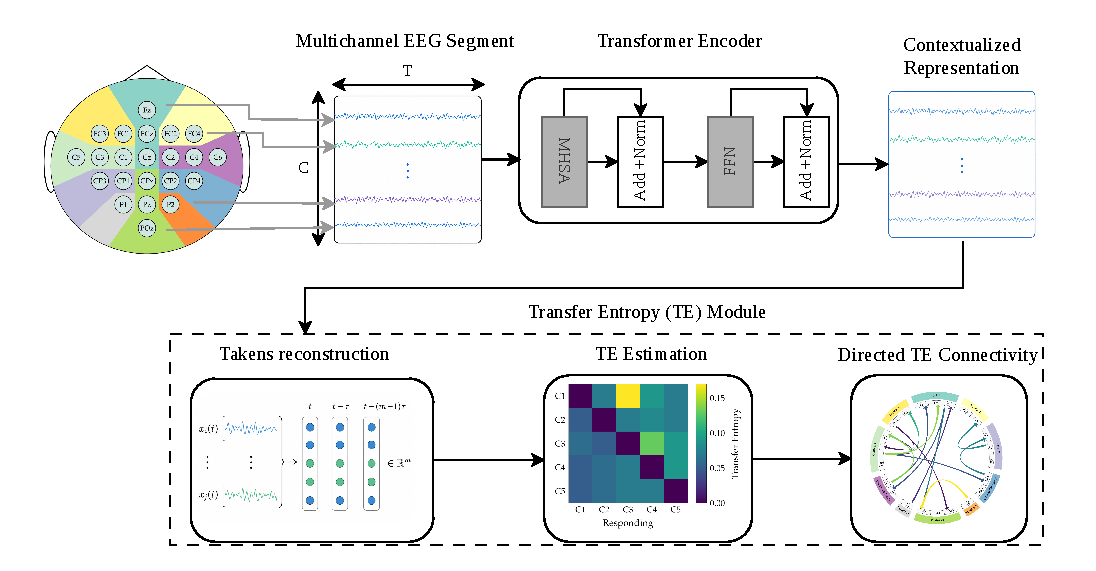
\includegraphics[width=\textwidth]{Figures/CTE-Net.pdf}
  \caption{Overview of the proposed framework for learning directed connectivity from multichannel \gls{eeg}. An input segment with $C$ channels and $T$ time samples is processed by a Transformer encoder comprising multi-head self-attention (MHSA), a feed-forward network (FFN), and residual connections with normalization (Add + Norm). The resulting contextualized representation enters the transfer entropy (TE) module, where Takens delay-coordinate reconstruction precedes the estimation of pairwise directed dependencies. These dependencies form a TE connectivity matrix, visualized as a directed connectivity graph.}
  \label{fig:tekte_pipeline}
\end{figure}

In this chapter, we extend the kernel-based TE paradigm to pediatric \gls{adhd} classification by proposing \gls{ctenet}, an end-to-end architecture that integrates Transformer-based contextualization with differentiable directed connectivity estimation. The model first processes each multichannel \gls{eeg} window using a Transformer encoder to obtain globally contextualized channel representations. These representations are then processed through channel-wise nonlinear temporal filters and Takens delay-coordinate embeddings. A differentiable kernel-based Transfer Entropy module estimates directed predictive information dependencies for all ordered electrode pairs, and the resulting connectivity representation is used for binary classification. In this manner, \gls{ctenet} combines global contextual modeling with nonlinear, time-delayed, and directed \gls{eeg} connectivity analysis.

Figure~\ref{fig:tekte_pipeline} illustrates the main processing stages of the proposed framework, from multichannel \gls{eeg} segments to directed-connectivity representations for \gls{adhd}-versus-control classification. A Transformer encoder produces contextualized representations, which are subsequently processed through Takens delay-coordinate reconstruction and transfer entropy estimation to characterize directed inter-channel dependencies.

\section{Materials and Methods}

{The original dataset comprised 61 participants with \gls{adhd} and 60 controls. To define a balanced cohort, one \gls{adhd} participant was randomly selected and excluded before window segmentation, fold construction, hyperparameter optimization, model training, and evaluation. The selection was not based on \gls{eeg} signal characteristics or quality, demographic or clinical information, model predictions, or classification performance. The resulting balanced cohort comprised 120 children, with 60 participants in the \gls{adhd} group and 60 in the control group, and was maintained across all models and experimental analyses.} The \gls{eeg} recordings were loaded in their original temporal form without applying additional artifact rejection, independent component analysis, frequency filtering, or spectral-band decomposition. This strategy was adopted to minimize preprocessing assumptions and allow the proposed network to learn temporal and connectivity-related patterns directly from the available multichannel recordings. As a post hoc signal-quality assessment, \gls{eeg} windows were screened for nonfinite values, flat channels, extreme amplitude, kurtosis, frontal low- and high-frequency activity, and 50-Hz line noise. Participant-balanced median/MAD thresholds were estimated from 30 windows per participant, with robust $z>5$ defining potentially contaminated windows. Without retraining, out-of-fold metrics were recalculated after excluding flagged windows and reaggregating participant probabilities; $z>4$ and $z>6$ were examined as sensitivity thresholds.

Each continuous recording was partitioned into 4-s windows, corresponding to 512 temporal samples at the original sampling frequency of 128~Hz. Consecutive windows were extracted with 50\% overlap; therefore, adjacent segments were separated by 256 samples, equivalent to a temporal shift of 2~s. The $n$-th \gls{eeg} segment was represented as

\begin{equation}
    \mathbf{X}^{(n)} \in \mathbb{R}^{C \times T},
\end{equation}

where $C=19$ is the number of \gls{eeg} channels and $T=512$ is the number of temporal samples per window. Each segment retained the diagnostic label and subject identifier associated with its original recording.

{The 50\% overlap increased temporal coverage and provided additional but partially redundant segments during model optimization; therefore, adjacent windows were not treated as independent statistical observations. Subject-wise partitioning kept all windows from each participant within a single training, validation, or test subset, preventing information leakage. Primary inference used one aggregated out-of-fold prediction per participant and participant-level bootstrap confidence intervals, while window-level metrics were interpreted as descriptive.}

{The number of windows per participant ranged from 30 to 167, with a median of 64 and an interquartile range of 51.75--77, yielding 8,213 windows in total. Participants with \gls{adhd} contributed 4,556 windows, with a median of 70.5 (IQR: 53.75--91.5), whereas controls contributed 3,657 windows, with a median of 59.5 (IQR: 51--68). Because training and window-level evaluation operated on individual windows, participants with longer recordings contributed more observations. Nevertheless, the primary participant-level evaluation assigned one aggregated out-of-fold prediction to each participant, giving all participants equal weight in the reported participant-level metrics.}

Subject identifiers were preserved throughout the experimental pipeline and subsequently used to construct the cross-validation partitions. Thus, all windows belonging to a given participant were assigned exclusively to a single training, validation, or test subset, preventing subject-level information leakage during model optimization and evaluation.
%------------------------------------------------------
\subsection{\gls{ctenet} Architecture}

\begin{table*}[htbp]
\centering
\caption{Compact \gls{ctenet} architecture for \gls{eeg}-based \gls{adhd} classification.}
\label{tab:model_architecture}

\small
\setlength{\tabcolsep}{5pt}
\renewcommand{\arraystretch}{1.17}

\begin{tabularx}{\textwidth}{@{}
    L{0.25\textwidth}
    L{0.13\textwidth}
    L{0.22\textwidth}
    Y
@{}}
\toprule
\textbf{Layer}
& \textbf{Variable}
& \textbf{Output dimension}
& \textbf{Configuration} \\
\midrule

\multicolumn{4}{@{}l}{\textbf{Block 1: Contextualization}} \\
\midrule

Input \gls{eeg}
& $\mat{X}$
& $C \times T$
& $C=19,\;T=512$ \\

Transpose
& $\mat{X}^{\top}$
& $T \times C$
& -- \\

Input projection
& $\mat{E}$
& $T \times d$
& {$d=128$} \\

Transformer encoder
& $\mat{H}$
& $T \times d$
& {$L=1,\;n_h=1,\;d_h=128,\;d_{ff}=128,\;p=0.5$} \\

Channel projection
& $\mat{X}_{f}^{\top}$
& $T \times C$
& $d\rightarrow C$ \\

Transpose
& $\mat{X}_{f}$
& $C \times T$
& -- \\

\midrule
\multicolumn{4}{@{}l}{\textbf{Block 2: Transfer Entropy}} \\
\midrule

Temporal filtering
& $\mat{\Phi}$
& $C \times T_{\phi}$
& {$K=83,\;T_{\phi}=107,\;s=1,\;\mathrm{pool}=4$} \\

Takens source state
& $\mat{Z}_{x^-}$
& $C \times T_z \times D_x$
& {$D_x=6,\;T_z=48$} \\

Takens target past
& $\mat{Z}_{y^-}$
& $C \times T_z \times D_y$
& {$D_y=1,\;T_z=48$} \\

Takens target present
& $\ve{z}_{y}$
& $C \times T_z \times 1$
& {$T_z=48$} \\

Kernel matrices
& $\mat{K}_{x^-},\,\mat{K}_{y^-},\,\mat{K}_{y}$
& {$19 \times 48 \times 48$}
& {$\tau=2,\;\mu=2,\;a=1,\;\ell=1,\;\alpha_{\mathrm{RQ}}=1$} \\

Transfer Entropy
& $\mat{TE}$
& $C \times C$
& $\alpha_{\mathrm{R}}=2$ \\

Flatten
& $\ve{h}_{TE}$
& $C(C-1)$
& -- \\

\midrule
\multicolumn{4}{@{}l}{\textbf{Block 3: Classification}} \\
\midrule

Dense
& $\ve{h}$
& $H$
& {$H=64$} \\

Dropout
& --
& {$64$}
& {$p=0.5$} \\

Output layer
& $\hat{y}$
& $O$
& $O=1$ \\

\bottomrule
\end{tabularx}
\end{table*}

% %----------------------------------------------------------------------------------

\subsubsection{Transformer-based contextualization}

Let a multichannel \gls{eeg} window be represented as $\mat{X}\in\mathbb{R}^{C\times T}$, where $C$ and $T$ denote the number of channels and temporal samples, respectively. Each temporal sample is treated as a sequence token containing the simultaneous activity of all \gls{eeg} channels. The normalized token sequence is projected onto a $d$-dimensional latent space as:

\begin{equation}
    \mat{E}
    =
    \operatorname{LN}_{C}\!\left(\mat{X}^{\top}\right)
    \mat{W}_{e}
    +
    \ve{b}_{e},
    \qquad
    \mat{E}\in\mathbb{R}^{T\times d}.
\end{equation}

A stack of $L$ standard Transformer encoder blocks \cite{vaswani2017attention}, comprising multi-head self-attention, feed-forward layers, residual connections, and layer normalization, produces

\begin{equation}
    \mat{H}
    =
    \operatorname{TrEnc}_{L}(\mat{E})
    \in\mathbb{R}^{T\times d}.
\end{equation}

The contextualized representation is projected back onto the original channel space:

\begin{equation}
    \mat{X}_{f}
    =
    \left[
        \operatorname{LN}(\mat{H})\mat{W}_{p}
        +
        \ve{b}_{p}
    \right]^{\top}
    \in\mathbb{R}^{C\times T}.
\end{equation}

Therefore, each row of $\mat{X}_{f}$ represents an \gls{eeg} channel contextualized using information from the complete temporal sequence and the remaining channels. The Transformer configuration is reported
in Table~\ref{tab:model_architecture}.

{No explicit positional encoding was incorporated into the Transformer encoder. Consequently, the self-attention mechanism does not, by itself, encode absolute temporal order or temporal distance based on token position. In \gls{ctenet}, self-attention is instead used as a content-based global contextualization mechanism, allowing each temporal sample to be represented in relation to the multichannel activity observed across the entire \gls{eeg} window. The resulting contextualized sequence remains indexed along the original time axis and is subsequently processed through channel-wise depthwise temporal convolution and Takens delay-coordinate reconstruction. These stages explicitly exploit temporal ordering and construct past and present states according to the reconstruction delay $\tau$ and the source--target interaction lag $\mu$. Thus, global content-based contextualization and the explicit modeling of ordered and delayed temporal dependencies are assigned to distinct components of the architecture.}

\subsubsection{Differentiable directed Transfer Entropy estimation}

The Transformer-contextualized signals are independently processed through channel-wise nonlinear temporal filters. The complete filtering operation is expressed as

\begin{equation}
    \mat{\Phi}
    =
    \operatorname{BN}
    \left[
        \operatorname{AvgPool}
        \left(
            \operatorname{ReLU}
            \left(
                \operatorname{DWConv1D}(\mat{X}_{f})
            \right)
        \right)
    \right]
    \in\mathbb{R}^{C\times T_{\phi}},
\end{equation}

where $\operatorname{DWConv1D}$ denotes a depthwise temporal convolution, so that each contextualized channel is filtered independently. The kernel size, stride, and pooling configuration are provided in
Table~\ref{tab:model_architecture}.

For each ordered source--target pair $(c,c')$, delay-coordinate embeddings are constructed from the filtered signals \cite{takens1981detecting}. At temporal anchor $t$, the source past, target past, and target present states are
defined as:

\begin{align}
    \ve{z}_{x_c^{-}}(t)
    &=
    \left[
        \phi_c(t-\mu-j\tau)
    \right]_{j=0}^{D_x-1}
    \in\mathbb{R}^{D_x},
    \\
    \ve{z}_{y_{c'}^{-}}(t)
    &=
    \left[
        \phi_{c'}(t-j\tau)
    \right]_{j=1}^{D_y}
    \in\mathbb{R}^{D_y},
    \\
    z_{y_{c'}}(t)
    &=
    \phi_{c'}(t).
\end{align}

Here, $D_x$ and $D_y$ are the source and target embedding dimensions, $\tau$ is the reconstruction delay, and $\mu$ represents the delayed source--target interaction.

Collecting the states over all valid temporal anchors yields $\mat{Z}_{x_c^{-}}$, $\mat{Z}_{y_{c'}^{-}}$, and $\mat{Z}_{y_{c'}}$. Before kernel evaluation, trainable bias-free
linear projections are applied:

\begin{equation}
    \widetilde{\mat{Z}}_{s}
    =
    \mat{Z}_{s}\mat{W}_{s},
    \qquad
    s\in
    \left\{
        x_c^{-},y_{c'}^{-},y_{c'}
    \right\}.
\end{equation}

For each projected state representation, a Gram matrix is constructed using the rational quadratic kernel \cite{rasmussen2006gaussian}. Specifically, for $s\in\{x_c^{-},y_{c'}^{-},y_{c'}\}$,

\begin{equation}
    \left[\mat{K}_{s}\right]_{ij}
    =
    \kappa_{\mathrm{RQ}}
    \left(
        \widetilde{\ve{z}}_{s,i},
        \widetilde{\ve{z}}_{s,j}
    \right)
    =
    a^{2}
    \left(
        1+
        \frac{
            \left\|
                \widetilde{\ve{z}}_{s,i}
                -
                \widetilde{\ve{z}}_{s,j}
            \right\|_{2}^{2}
        }{
            2\alpha_{\mathrm{RQ}}\ell^{2}
        }
    \right)^{-\alpha_{\mathrm{RQ}}},
\end{equation}

where $a$, $\ell$, and $\alpha_{\mathrm{RQ}}$ denote the kernel amplitude, length scale, and scale-mixture parameter, respectively.
The resulting matrices
$\mat{K}_{x_c^{-}}$, $\mat{K}_{y_{c'}^{-}}$, and $\mat{K}_{y_{c'}}$ encode pairwise similarities between the reconstructed states at the valid temporal anchors. The kernel configuration is reported in Table~\ref{tab:model_architecture}.
{For positive kernel parameters, the Rational Quadratic kernel produces positive-semidefinite Gram matrices. Moreover, the Hadamard products used to construct the joint kernel representations preserve positive semidefiniteness.}

{Numerical stability was ensured by enforcing strictly positive kernel parameters and using $\varepsilon=10^{-8}$ as a lower bound for the kernel length scale $\ell$ and shape parameter $\alpha_{\mathrm{RQ}}$, as well as a stabilizing constant during trace normalization and logarithmic entropy evaluation.}

For a positive semidefinite matrix $\mat{A}$, let the trace-normalization operator be defined as:

\begin{equation}
    \mathcal{N}(\mat{A})
    =
    \frac{\mat{A}}
    {\operatorname{tr}(\mat{A})}.
\end{equation}

The matrix-based R\'enyi entropy of order $\alpha_{\mathrm{R}}$ is then defined as:

\begin{equation}
    H_{\alpha_{\mathrm{R}}}(\mat{A})
    =
    \frac{1}{1-\alpha_{\mathrm{R}}}
    \log
    \left[
        \operatorname{tr}
        \left(
            \mathcal{N}(\mat{A})^{\alpha_{\mathrm{R}}}
        \right)
    \right].
\end{equation}
{This matrix-based entropy functional follows the positive definite kernel formulation introduced for information-theoretic learning and subsequently used for kernel-based Transfer Entropy estimation \cite{sanchezgiraldo2015entropy,delapava2019renyiTE}.}

For multiple variables represented by Gram matrices $\mat{K}_{1},\ldots,\mat{K}_{M}$, the corresponding joint entropy is computed from their Hadamard product:

\begin{equation}
    H_{\alpha_{\mathrm{R}}}
    \left(
        \mat{K}_{1},\ldots,\mat{K}_{M}
    \right)
    =
    H_{\alpha_{\mathrm{R}}}
    \left(
        \mat{K}_{1}
        \odot\cdots\odot
        \mat{K}_{M}
    \right),
\end{equation}

where $\odot$ denotes the Hadamard product. The trace normalization included in $H_{\alpha_{\mathrm{R}}}(\cdot)$ ensures that both marginal and joint kernel representations have unit trace before evaluating the entropy.

Accordingly, the directed Transfer Entropy from source channel $c$ to target channel $c'$ is computed as

\begin{align}
    TE_{c\rightarrow c'}
    ={}&
    H_{\alpha_{\mathrm{R}}}
    \left(
        \mat{K}_{y_{c'}^{-}},
        \mat{K}_{x_c^{-}}
    \right)
    -
    H_{\alpha_{\mathrm{R}}}
    \left(
        \mat{K}_{y_{c'}},
        \mat{K}_{y_{c'}^{-}},
        \mat{K}_{x_c^{-}}
    \right)
    \nonumber\\
    &+
    H_{\alpha_{\mathrm{R}}}
    \left(
        \mat{K}_{y_{c'}},
        \mat{K}_{y_{c'}^{-}}
    \right)
    -
    H_{\alpha_{\mathrm{R}}}
    \left(
        \mat{K}_{y_{c'}^{-}}
    \right).
\end{align}

Repeating this computation over all ordered channel pairs produces the directed connectivity matrix

\begin{equation}
    \mat{TE}
    =
    \left[
        TE_{c\rightarrow c'}
    \right]_{c,c'=1}^{C}
    \in\mathbb{R}^{C\times C}.
\end{equation}

Since the source and target states have different roles in the formulation, $\mat{TE}$ is generally asymmetric. Therefore, its coefficients represent directed predictive information dependencies
between Transformer-contextualized \gls{eeg} channels rather than undirected similarity relationships. {Although theoretical Transfer Entropy is non-negative, the present matrix-based formulation is a finite-sample estimator and does not explicitly enforce non-negativity. Consequently, negative estimates may occur and should not be interpreted as negative information transfer. Furthermore, because the Transformer, temporal filters, and linear projections preceding the TE module are optimized end-to-end using the supervised classification objective, the resulting coefficients quantify directed predictive dependencies within the learned representation space rather than conventional Transfer Entropy estimated directly from the raw \gls{eeg}. Accordingly, a labeled coefficient such as F8$\rightarrow$C4 denotes a directed dependency between channel-indexed coordinates of the learned contextualized representation and should not be interpreted as conventional Transfer Entropy between the original F8 and C4 electrode signals or as a source-level cortical interaction.}


\subsubsection{Connectivity-based classification}

The diagonal coefficients of $\mat{TE}$ represent self-connections and are excluded from the classification representation. The remaining directed coefficients are vectorized as

\begin{equation}
    \ve{h}_{\mathrm{TE}}
    =
    \operatorname{vec}
    \left(
        \left\{
            TE_{c\rightarrow c'}
            \mid
            c\neq c'
        \right\}
    \right)
    \in\mathbb{R}^{C(C-1)}.
\end{equation}

The resulting connectivity vector is processed by a fully connected classification head, and the estimated probability of \gls{adhd} is given by

\begin{equation}
    \hat{y}
    =
    \sigma
    \left[
        \ve{w}_{o}^{\top}
        \operatorname{Dropout}_{p_d}
        \left(
            \operatorname{ReLU}
            \left(
                \mat{W}_{h}\ve{h}_{\mathrm{TE}}
                +
                \ve{b}_{h}
            \right)
        \right)
        +
        b_o
    \right],
\end{equation}

where $\sigma(\cdot)$ denotes the sigmoid function and $p_d$ is the dropout probability. The complete architecture is optimized end-to-end using binary cross-entropy evaluated directly from the classification logits.

\subsection{Training Strategy and Evaluation Protocol}
\label{subsec:training_evaluation}

\gls{ctenet} was evaluated using five-fold stratified group cross-validation, with each participant treated as an independent group. At each iteration, 24 participants were held out for testing, while the remaining participants were divided into subject-independent training and validation subsets. Thus, no participant contributed windows to more than one subset, and each participant appeared once in the test set.

{The model was trained end-to-end at the window level using binary cross-entropy. A single hyperparameter configuration was selected through 20 Optuna trials \cite{akiba2019optuna}, using the mean validation accuracy across the five predefined subject-wise folds as the optimization objective. Within each fold, training, validation, and test participants were mutually exclusive, and only the corresponding validation subset guided early stopping and checkpoint selection. No test-set performance metric was included in hyperparameter optimization. The selected configuration, reported in Table~\ref{tab:model_architecture}, was then fixed for all five folds and all ten random training repetitions. Standardization and PCA were restricted to the post hoc representation analysis and did not influence model training, hyperparameter selection, or classification predictions.}

{Within the Transfer Entropy module, $D_x$, $D_y$, $\tau$, and $\mu$ were tuned through the 20-trial Optuna study over the ranges $D_x,D_y\in[1,10]$, $\tau\in[1,5]$, and $\mu\in[0,10]$. The selected values were $D_x=6$, $D_y=1$, $\tau=2$, and $\mu=2$. The Rényi order $\alpha_{\mathrm{R}}=2$ and the Rational Quadratic kernel parameters $a=\ell=\alpha_{\mathrm{RQ}}=1$ were fixed, whereas the linear projections preceding kernel evaluation were learned end-to-end.}

{A post hoc joint sensitivity analysis was conducted for $D_x$, $D_y$,
$\tau$, and $\mu$, as these parameters directly determine the temporal
organization of the reconstructed states and have shown relevant sensitivity
in related Takens-based kernel Transfer Entropy architectures
\cite{gomezrivera2025tektenet}. The originally selected configuration and ten feasible alternatives were evaluated across the five predefined subject-wise folds to characterize their combined sensitivity.}

The complete five-fold procedure was repeated using ten random seeds and identical subject partitions, resulting in 50 trained models. {The final \gls{ctenet} configuration contained 128,578 trainable parameters, corresponding to approximately 0.49~MiB of parameter storage in FP32. All experiments were conducted on the same workstation equipped with an NVIDIA Quadro RTX 5000 GPU, an eight-core CPU with 16 processing threads, and 16~GB of system RAM. The available execution records indicated approximate training times of 5--7 minutes per fold and 25--35 minutes for one complete five-fold repetition, while the complete 20-trial Optuna study required approximately 8.1 hours. For each \gls{eeg} window, the Transfer Entropy module evaluated all $C(C-1)=342$ ordered electrode pairs, excluding self-connections.} \gls{adhd} was considered the positive class, and window-level predictions were obtained using a probability threshold of 0.5. Performance was quantified as

\begin{equation}
\begin{aligned}
\mathrm{Accuracy}
&=\frac{\mathrm{TP}+\mathrm{TN}}
        {\mathrm{TP}+\mathrm{TN}+\mathrm{FP}+\mathrm{FN}},
&
\mathrm{Precision}
&=\frac{\mathrm{TP}}{\mathrm{TP}+\mathrm{FP}},
&
\mathrm{Sensitivity}
&=\frac{\mathrm{TP}}{\mathrm{TP}+\mathrm{FN}}.
\end{aligned}
\label{eq:classification_metrics}
\end{equation}

For each seed, metrics were averaged across the five test folds and reported as the mean and standard deviation across the ten seeds. \gls{ctenet} and the baselines were compared using paired two-sided Wilcoxon signed-rank tests with Holm correction {\cite{holm1979sequentially}}.

{These seed-based comparisons were retained as an exploratory assessment of the computational variability associated with repeated model training. The random seeds were not interpreted as independent clinical observations. Participant-level performance and uncertainty were therefore evaluated separately using the participants as the sampling units, as described below.}

{For the participant-level evaluation, the out-of-fold \gls{adhd} probabilities assigned to all windows belonging to participant $s$ under random training seed $r$ were averaged as}

\begin{equation}
{
\bar{p}_{s}^{(r)}
=
\frac{1}{N_s}
\sum_{i=1}^{N_s}
p_{s,i}^{(r)}
}
\label{eq:participant_probability}
\end{equation}

{where $N_s$ is the number of windows available for participant $s$ and $p_{s,i}^{(r)}$ is the \gls{adhd} probability assigned to window $i$. A participant was classified as \gls{adhd} when $\bar{p}_{s}^{(r)} \geq 0.5$ and as control otherwise. Accuracy, sensitivity, specificity, precision, and F1-score were calculated from the resulting participant-level decisions, whereas ROC-AUC was calculated directly from the continuous participant-level probabilities.}

{The participant-level metrics were calculated separately for each of the ten random training seeds using the 120 out-of-fold participants. Point estimates were subsequently obtained by averaging the corresponding metric across the ten seeds. The seeds were regarded as repeated model fits representing optimization variability and were not treated as independent clinical observations. Ninety-five percent confidence intervals were estimated using 5,000 stratified percentile bootstrap resamples at the participant level \cite{efron1979bootstrap}. Within each bootstrap replicate, control and \gls{adhd} participants were resampled separately with replacement, the same resampled participant indices were applied across all ten seeds, and the resulting seed-specific metrics were averaged.}

{All baseline architectures were trained and evaluated under the same experimental protocol as \gls{ctenet}, using identical training, validation, and test participant assignments, input windows, raw \gls{eeg} preprocessing, hyperparameter-tuning budget of 20 Optuna trials, validation-based early-stopping and checkpoint-selection criteria, and ten random training repetitions per fold. Although the hyperparameter search spaces were architecture-specific, the same optimization budget and validation objective were applied to every model.}

{Both ablation variants were evaluated using the same fixed subject-wise folds and ten random seeds as \gls{ctenet}. Seed-level differences were assessed using paired Wilcoxon signed-rank tests with Holm correction across six comparisons. For the participant-level analysis, one consensus decision per participant and model was obtained by averaging the out-of-fold probabilities across seeds and applying a threshold of 0.5. Exact McNemar tests \cite{mcnemar1947sampling} were then performed with Holm correction across the two ablation comparisons.}

{Sensitivity of predictive performance and learned connectivity to preprocessing and reference choice was assessed by retraining \gls{ctenet} using frequency-filtered and quality-screened \gls{eeg} or common average reference. Both analyses used the fixed configuration, five subject-wise folds, and ten seeds without additional hyperparameter optimization. Complete methods and results are provided in Supplementary Data~S4.}
\subsection{Representation Analysis}
\label{subsec:representation_analysis}

The original \gls{eeg}, Transformer output $\mat{X}_{f}$, temporal-filter output $\mat{\Phi}$, and Transfer Entropy representation were extracted exclusively from out-of-fold test windows. Each representation was vectorized, standardized within each seed--fold execution, and projected onto 30 principal components for the main analysis.

Let $\ve{z}_{s,i}^{(\ell,r)}$ denote the representation of window $i$ from participant $s$, at stage $\ell$ and repetition $r$. Within-subject dispersion and its change relative to the original \gls{eeg} were computed as:

\begin{equation}
\begin{aligned}
\boldsymbol{\mu}_{s}^{(\ell,r)}
&=\frac{1}{N_s}\sum_{i=1}^{N_s}\ve{z}_{s,i}^{(\ell,r)},
&
D_s^{(\ell,r)}
&=\frac{1}{N_s}\sum_{i=1}^{N_s}
\left\|
\ve{z}_{s,i}^{(\ell,r)}
-\boldsymbol{\mu}_{s}^{(\ell,r)}
\right\|_2,
\\
\widetilde{D}_s^{(\ell,r)}
&=\frac{D_s^{(\ell,r)}}{G^{(\ell,r)}},
&
\Delta_s^{(\ell)}
&=100\left(
\frac{\widetilde{D}_s^{(\ell)}}
     {\widetilde{D}_s^{(\mathrm{\gls{eeg}})}}
-1\right),
\end{aligned}
\label{eq:representation_dispersion}
\end{equation}

where $N_s$ is the number of windows and $G^{(\ell,r)}$ is the mean pairwise Euclidean distance among at most 1,200 test windows in the corresponding representation space. Participant-level dispersion was averaged across seeds before statistical analysis. Lower $\widetilde{D}_s^{(\ell,r)}$ values indicate more compact within-subject representations, whereas negative $\Delta_s^{(\ell)}$ values indicate a reduction relative to raw \gls{eeg}. These quantities describe representation-space dispersion rather than physiological \gls{eeg} variability.

Diagnostic organization was evaluated using the \gls{adhd}--control silhouette coefficient at the window level, the diagnostic silhouette of participant centroids \cite{rousseeuw1987silhouettes}, and the ratio $R=\overline{d}_{\mathrm{same}}/\overline{d}_{\mathrm{different}}$ between same-class and different-class centroid distances. Higher silhouette values and lower ratios indicate better diagnostic organization.

Finally, TE stability was evaluated by comparing each window-level connectivity vector with the mean of the remaining windows from the same participant. Spearman correlation measured the stability of the global connection ranking, while Jaccard similarity measured the overlap between the strongest 10\% of directed connections. Both measures were averaged across windows and seeds to obtain one value per participant.

Participant-level dispersion values were averaged across seeds and compared among stages using the Friedman test, followed by paired Wilcoxon signed-rank tests with Holm correction. Effect sizes were quantified using matched rank-biserial correlations, and 95\% confidence intervals were estimated from 5,000 participant-level bootstrap resamples. Robustness was assessed by repeating the analysis with 15, 30, and 60 PCA components and using pairwise cosine distance without PCA. Diagnostic-organization metrics were averaged across folds within each seed and analyzed using the same paired procedure.

{For each representation stage, the standardization mean and standard deviation and the PCA basis were computed independently from the pooled out-of-fold test windows of that stage and seed-fold, prior to projection onto the leading 30 components. Because this fitting is representation-specific,  we repeated the dispersion analysis using pairwise cosine distance on the standardized features without PCA, confirming that the reduction in within-subject dispersion is not an artifact of the per-representation standardization or PCA basis.}

%----------------------------------------------------------
\subsection{Results and Discussion}
\label{sec:results_and_discussion}
%----------------------------------------------------------
\gls{ctenet} was evaluated under the subject-independent protocol described in Section~\ref{subsec:training_evaluation}. The results examine four complementary aspects of the proposed architecture: classification performance and statistical comparison, model robustness and sensitivity, the organization and stability of the learned representation space, and subject-specific directed-connectivity patterns associated with correct and incorrect classification decisions.

\subsubsection{Classification Performance and Statistical Comparison}\label{subsec:classification_performance}

%----------------------------------------------------------
\begin{table}[htbp]
\centering
\caption{Window-level classification performance of \gls{ctenet} and the baseline models. Results are reported as the mean and sample standard deviation across ten random training seeds after averaging the five test folds within each seed.}
\label{tab:window_level_models}

\begin{threeparttable}
\scriptsize
\renewcommand{\arraystretch}{1.15}
\setlength{\tabcolsep}{3pt}

\begin{tabular*}{\textwidth}{@{\extracolsep{\fill}}l
    S[table-format=2.1]@{\,$\pm$\,}S[table-format=1.1]
    S[table-format=2.1]@{\,$\pm$\,}S[table-format=1.1]
    S[table-format=2.1]@{\,$\pm$\,}S[table-format=1.1]
    S[table-format=2.1]@{\,$\pm$\,}S[table-format=1.1]
    S[table-format=2.1]@{\,$\pm$\,}S[table-format=1.1]
    S[table-format=2.1]@{\,$\pm$\,}S[table-format=1.1]
    S[table-format=2.1]@{\,$\pm$\,}S[table-format=1.1]@{}}
\toprule

\multirow{2}{*}{\textbf{Model}}
& \multicolumn{4}{c}{\textbf{Overall}}
& \multicolumn{8}{c}{\textbf{Class-specific}}
& \multicolumn{2}{c}{\textbf{Ranking}} \\

\cmidrule(lr){2-5}\cmidrule(lr){6-13}\cmidrule(l){14-15}

& \multicolumn{2}{c}{\textbf{Accuracy}}
& \multicolumn{2}{c}{\textbf{BAcc}}
& \multicolumn{2}{c}{\textbf{Sens.}}
& \multicolumn{2}{c}{\textbf{Spec.}}
& \multicolumn{2}{c}{\textbf{Prec.}}
& \multicolumn{2}{c}{\textbf{F1}}
& \multicolumn{2}{c}{\textbf{ROC-AUC}} \\

\midrule

\rowproposed
\textbf{CTE-Net}
& 80.9 & 1.7 & 80.6 & 1.8 & 84.2 & 2.3 & 77.0 & 3.2 & 82.7 & 2.1 & 82.9 & 1.5 & 87.9 & 1.5 \\

\gls{eeg}Net
& 81.5 & 2.1 & 81.4 & 2.1 & 83.5 & 3.6 & 79.3 & 4.0 & 84.3 & 2.2 & 83.1 & 2.2 & 88.8 & 2.5 \\

ShallowConvNet
& \bfseries 83.5 & \bfseries 1.7 & \bfseries 83.7 & \bfseries 1.8 & 80.6 & 2.4 & \bfseries 86.9 & \bfseries 3.4 & \bfseries 88.1 & \bfseries 2.9 & \bfseries 83.2 & \bfseries 2.0 & \bfseries 90.4 & \bfseries 1.7 \\

T-GARNet
& 77.6 & 0.5 & 76.7 & 0.6 & 85.6 & 1.1 & 67.8 & 1.9 & 77.3 & 0.8 & 80.8 & 0.4 & 84.0 & 0.4 \\

IMC-BGT
& 66.3 & 1.2 & 65.3 & 1.4 & 74.7 & 2.7 & 55.8 & 4.5 & 68.2 & 1.6 & 70.8 & 1.0 & 71.2 & 1.0 \\

MultiStream
& 58.6 & 0.3 & 55.2 & 0.4 & \bfseries 86.1 & \bfseries 0.9 & 24.4 & 1.4 & 58.7 & 0.3 & 69.8 & 0.3 & 55.3 & 0.4 \\

\bottomrule
\end{tabular*}

\begin{tablenotes}[flushleft]
\footnotesize
\item \textit{Note:} All values are percentages. \gls{adhd} was treated as the
positive class, so sensitivity denotes the true-positive rate for \gls{adhd} and
specificity the true-negative rate for controls. BAcc denotes balanced
accuracy. Values were first averaged across the five test folds within each
seed and then summarized across the ten random training seeds. The seeds
represent repeated model fits and were not treated as independent clinical
observations. The shaded row indicates the proposed model, and bold values
indicate the highest point estimate for each metric.
\end{tablenotes}
\end{threeparttable}
\end{table}
%----------------------------------------------------------
{Classification performance was examined from two complementary statistical perspectives. First, the seed-level analysis characterized the variability associated with repeated model optimization under the same fixed subject-wise partitions. Mean and standard deviation across the ten random seeds were reported, and paired Wilcoxon signed-rank tests with Holm correction were used to assess whether the observed performance differences were consistent across repeated model fits. Because the subject partitions were reused, this analysis was interpreted as an assessment of optimization stability and not as inference based on independent clinical observations. Second, participant-level performance was evaluated using out-of-fold predictions, participant-level bootstrap confidence intervals, and exact paired McNemar tests, thereby treating the participant as the primary unit for evaluating generalization.}

{Table~\ref{tab:window_level_models} presents the complete window-level classification performance of \gls{ctenet} and the baseline models. In addition to accuracy, precision, and sensitivity, specificity, balanced accuracy, F1-score, and ROC-AUC are reported to provide a more complete assessment of class-specific behavior. These complementary metrics are particularly relevant for identifying models whose performance may be driven by a tendency to favor the \gls{adhd} class.}

{The window-level results reveal distinct classification profiles among the evaluated models. ShallowConvNet achieved the strongest overall point-estimate profile, leading in accuracy, balanced accuracy, specificity, precision, F1-score, and ROC-AUC, although it exhibited lower sensitivity than \gls{ctenet}. \gls{ctenet} and \gls{eeg}Net showed similarly competitive and comparatively balanced performance across the evaluated metrics, indicating that their classification results were not predominantly driven by either diagnostic class. In contrast, T-GARNet exhibited higher sensitivity but lower specificity and precision, suggesting a greater tendency to classify windows as \gls{adhd}. This behavior was even more pronounced for MultiStream, whose high sensitivity was accompanied by markedly lower specificity, balanced accuracy, precision, and ROC-AUC. IMC-BGT also showed a less balanced performance profile. Overall, these results demonstrate why sensitivity should be interpreted jointly with specificity, balanced accuracy, F1-score, and ROC-AUC when comparing the models.}

{The row-normalized window-level confusion matrices for all evaluated models are provided in Supplementary Data~S1. These matrices complement the reported class-specific metrics and facilitate inspection of each model's tendency to classify windows as \gls{adhd} or control.}

{To complement this descriptive performance analysis, the consistency of the differences between \gls{ctenet} and the baseline models across repeated training runs was examined using paired Wilcoxon signed-rank tests with Holm correction. These exploratory seed-level comparisons are reported in
Table~\ref{tab:ctenet_posthoc}.}

{Within the exploratory seed-level analysis, \gls{ctenet} and \gls{eeg}Net showed comparable accuracy, precision, and sensitivity across repeated model fits. ShallowConvNet achieved higher point estimates for accuracy and precision; however, only the precision difference remained significant after Holm correction. \gls{ctenet} showed consistently higher accuracy and precision than T-GARNet, IMC-BGT, and MultiStream. For sensitivity, \gls{ctenet} significantly outperformed only IMC-BGT, whereas no significant differences were found relative to \gls{eeg}Net, ShallowConvNet, T-GARNet, or MultiStream. Overall, these results indicate that \gls{ctenet} provides a stable balance among accuracy, precision, and sensitivity across repeated model fits.}
%----------------------------------------------------------
\begin{table}[htbp]
\centering
\caption{Exploratory seed-level comparisons between \gls{ctenet} and the
baseline models. Results are reported as the mean and standard deviation
across ten random training seeds. Paired Wilcoxon signed-rank tests were
used to evaluate the consistency of the differences across repeated
model fits, with Holm correction applied jointly across the 15
comparisons. Random seeds were treated as computational repetitions and
not as independent clinical observations.}
\label{tab:ctenet_posthoc}
\begin{threeparttable}
\scriptsize
\renewcommand{\arraystretch}{1.2}
\setlength{\tabcolsep}{3pt}
\begin{tabular*}{\textwidth}{@{\extracolsep{\fill}}l
    S[table-format=2.1]@{\,$\pm$\,}S[table-format=1.1] S[table-format=1.4] c
    S[table-format=2.1]@{\,$\pm$\,}S[table-format=1.1] S[table-format=1.4] c
    S[table-format=2.1]@{\,$\pm$\,}S[table-format=1.1] S[table-format=1.4] c@{}}
\toprule

\multirow{2}{*}{\textbf{Model}}
& \multicolumn{4}{c}{\textbf{Accuracy (\%)}}
& \multicolumn{4}{c}{\textbf{Precision (\%)}}
& \multicolumn{4}{c}{\textbf{Sensitivity (\%)}} \\

\cmidrule(lr){2-5}\cmidrule(lr){6-9}\cmidrule(l){10-13}

& \multicolumn{2}{c}{Mean\,$\pm$\,SD} & {$p_{\mathrm{Holm}}$} & vs.
& \multicolumn{2}{c}{Mean\,$\pm$\,SD} & {$p_{\mathrm{Holm}}$} & vs.
& \multicolumn{2}{c}{Mean\,$\pm$\,SD} & {$p_{\mathrm{Holm}}$} & vs. \\

\midrule

\rowproposed
\textbf{\gls{ctenet}}
& \textbf{80.9} & \textbf{1.7} & {--} & --
& \textbf{82.7} & \textbf{2.1} & {--} & --
& \textbf{84.2} & \textbf{2.3} & {--} & -- \\

\gls{eeg}Net
& 81.5 & 2.1 & 1.0000 & $\approx$
& 84.3 & 2.2 & 0.7734 & $\approx$
& 83.5 & 3.6 & 1.0000 & $\approx$ \\

ShallowConvNet
& \bfseries 83.5 & \bfseries 1.7 & 0.0684 & $\approx$
& \bfseries 88.1 & \bfseries 2.9 & 0.0293 & $<$
& 80.6 & 2.4 & 0.0820 & $\approx$ \\

T-GARNet
& 77.6 & 0.5 & 0.0293 & $>$
& 77.3 & 0.8 & 0.0293 & $>$
& 85.6 & 1.1 & 0.7734 & $\approx$ \\

IMC-BGT
& 66.3 & 1.2 & 0.0293 & $>$
& 68.2 & 1.6 & 0.0293 & $>$
& 74.7 & 2.7 & 0.0293 & $>$ \\

MultiStream
& 58.6 & 0.3 & 0.0293 & $>$
& 58.7 & 0.3 & 0.0293 & $>$
& \bfseries 86.1 & \bfseries 0.9 & 0.5273 & $\approx$ \\

\bottomrule
\end{tabular*}
\begin{tablenotes}[flushleft]
\footnotesize
\item \textit{Note:} All values are percentages. The shaded row shows
\gls{ctenet}'s own results, which serve as the reference for every comparison;
the ``vs.'' columns therefore contrast each baseline with \gls{ctenet}. The
symbols $>$ and $<$ indicate a Holm-adjusted difference across repeated
model fits in favor of \gls{ctenet} or the compared model, respectively;
$\approx$ indicates that no difference was detected. Bold values indicate
the highest point estimate for each metric. These comparisons characterize
optimization variability and should not be interpreted as participant-level
evidence of model superiority. Primary participant-level comparisons are
reported in Table~\ref{tab:participant_mcnemar}.
\end{tablenotes}
\end{threeparttable}
\end{table}
%----------------------------------------------------------

{Because \gls{adhd} diagnosis and the intended generalization unit correspond to the participant rather than to individual \gls{eeg} windows, performance was additionally evaluated after aggregating the out-of-fold window probabilities within each participant. Table~\ref{tab:subject_level_models} reports the resulting participant-level point estimates and 95\% confidence intervals for all evaluated models. The point estimates summarize performance across the ten repeated model fits, whereas the confidence intervals were obtained by resampling participants and therefore quantify uncertainty with respect to the study cohort.}

%----------------------------------------------------------
\begin{table}[htbp]
\centering
\caption{Participant-level classification performance of \gls{ctenet} and the baseline models. Point estimates correspond to the mean participant-level performance across ten random training seeds. The 95\% confidence intervals were estimated using 5,000 stratified bootstrap resamples with the participant as the resampling unit.}
\label{tab:subject_level_models}

\begin{threeparttable}
\scriptsize
\renewcommand{\arraystretch}{1.25}
\setlength{\tabcolsep}{3pt}

\begin{tabular*}{\textwidth}{@{\extracolsep{\fill}}lcccccc@{}}
\toprule

\multirow{2}{*}{\textbf{Model}}
& \multicolumn{2}{c}{\textbf{Overall}}
& \multicolumn{3}{c}{\textbf{Class-specific}}
& \multicolumn{1}{c}{\textbf{Ranking}} \\

\cmidrule(lr){2-3}\cmidrule(lr){4-6}\cmidrule(l){7-7}

& \textbf{Accuracy}
& \textbf{F1-score}
& \textbf{Sensitivity}
& \textbf{Specificity}
& \textbf{Precision}
& \textbf{ROC-AUC} \\

\midrule

\makecell{\textbf{CTE-Net}}
& \ci{83.4}{78.2--88.2}
& \ci{83.8}{78.7--88.4}
& \ci{86.0}{79.0--92.0}
& \ci{80.8}{73.2--87.7}
& \ci{81.8}{76.1--87.6}
& \ci{90.2}{85.1--94.6} \\

\makecell{\gls{eeg}Net}
& \ci{82.7}{77.7--87.3}
& \ci{83.4}{78.6--87.8}
& \ci{87.2}{80.5--92.7}
& \ci{78.2}{70.3--85.2}
& \ci{80.1}{74.5--85.8}
& \ci{89.2}{83.5--93.9} \\

\makecell{ShallowConvNet}
& \ci{\textbf{84.7}}{79.2--89.8}
& \ci{\textbf{84.4}}{78.3--89.7}
& \ci{82.5}{74.0--90.2}
& \ci{\textbf{87.0}}{80.0--92.8}
& \ci{\textbf{86.5}}{80.5--92.3}
& \ci{\textbf{91.6}}{86.6--95.7} \\

\makecell{T-GARNet}
& \ci{79.4}{72.5--85.8}
& \ci{81.4}{75.6--87.0}
& \ci{90.3}{82.5--96.8}
& \ci{68.5}{57.0--79.3}
& \ci{74.2}{67.6--81.4}
& \ci{85.8}{78.2--92.5} \\

\makecell{IMC-BGT}
& \ci{72.7}{66.3--78.8}
& \ci{75.8}{70.1--81.0}
& \ci{85.3}{77.0--92.3}
& \ci{60.0}{50.0--70.0}
& \ci{68.3}{62.7--74.4}
& \ci{78.6}{70.2--86.2} \\

\makecell{MultiStream}
& \ci{56.2}{51.2--61.4}
& \ci{68.2}{64.8--71.4}
& \ci{\textbf{93.7}}{88.3--98.0}
& \ci{18.8}{10.2--28.3}
& \ci{53.6}{50.6--56.8}
& \ci{60.3}{50.9--69.6} \\

\bottomrule
\end{tabular*}

\begin{tablenotes}[flushleft]
\footnotesize
\item \textit{Note:} All values are percentages; 95\% confidence intervals are
given in parentheses. For each participant and random seed, window-level \gls{adhd}
probabilities were averaged and a threshold of 0.5 was applied to obtain the
participant-level decision. Confidence intervals were calculated with the
participant as the resampling unit and quantify uncertainty around each model
separately; they should not be interpreted as tests of pairwise differences,
which are reported in Table~\ref{tab:participant_mcnemar}. The ten seeds
represent repeated model fits and were not treated as independent clinical
observations. Seed-level mean and standard deviation are reported separately
in Table~\ref{tab:ctenet_posthoc} as descriptive measures of optimization
variability. \gls{ctenet}, the proposed model, is listed first and set in bold;
bold values indicate the highest point estimate for each metric.
\end{tablenotes}
\end{threeparttable}
\end{table}
% %----------------------------------------------------------

{At the participant level, ShallowConvNet exhibited the strongest overall point-estimate profile, whereas \gls{ctenet} followed closely and achieved the second-highest accuracy, specificity, precision, F1-score, and ROC-AUC. \gls{eeg}Net also showed a competitive overall performance. In contrast, T-GARNet favored sensitivity at the expense of specificity and precision. This imbalance was more pronounced for IMC-BGT and particularly for MultiStream, indicating a greater tendency to classify participants as \gls{adhd}.}

{The participant-level estimates show that \gls{ctenet} maintained robust and comparatively balanced discrimination when each participant, rather than each \gls{eeg} window, was treated as the evaluation unit. Its joint sensitivity and specificity indicate that its performance was not driven exclusively by the classification of one diagnostic group. Nevertheless, the confidence intervals in Table~\ref{tab:subject_level_models} quantify uncertainty around each model separately and should not be interpreted as tests of pairwise differences. Formal paired comparisons were therefore conducted using the predictions obtained for the same participants.}

{To determine whether the descriptive performance differences translated into different classification outcomes for the same participants, one consensus decision was obtained for each participant and model by averaging the corresponding out-of-fold probabilities across the ten random seeds and applying the 0.5 threshold. \gls{ctenet} was then compared with each baseline using the exact McNemar test, with Holm correction across the five comparisons. Unlike the exploratory Wilcoxon analysis, this paired analysis used participants, rather than random seeds, as the units of comparison.}

% %----------------------------------------------------------
\begin{table}[H]
\centering
\caption{Exact participant-level McNemar comparisons between \gls{ctenet} and the baseline models. Consensus decisions were obtained by averaging each participant's out-of-fold probabilities across the ten random training seeds and applying a threshold of 0.5.}
\label{tab:participant_mcnemar}

\begin{threeparttable}
\small
\renewcommand{\arraystretch}{1.15}
\setlength{\tabcolsep}{5pt}

\begin{tabular*}{\textwidth}{@{\extracolsep{\fill}}l
    S[table-format=2.0]S[table-format=2.0]
    cc l@{}}
\toprule

\multirow{2}{*}{\textbf{Baseline}}
& \multicolumn{2}{c}{\textbf{Discordant participants}}
& \multicolumn{2}{c}{\textbf{Exact McNemar test}}
& \multirow{2}{*}{\textbf{vs.\ CTE-Net}} \\

\cmidrule(lr){2-3}\cmidrule(lr){4-5}

& {\boldmath$n_{10}$}
& {\boldmath$n_{01}$}
& \boldmath{$p_{\mathrm{exact}}$}
& \boldmath{$p_{\mathrm{Holm}}$}
& \\

\midrule

\gls{eeg}Net          &  8 & 7 & 1.0000 & 1.0000 & $\approx$ \\
ShallowConvNet  & 12 & 9 & 0.6636 & 1.0000 & $\approx$ \\
T-GARNet        & 12 & 3 & 0.0352 & 0.1055 & $\approx$ \\
IMC-BGT         & 21 & 7 & 0.0125 & 0.0502 & $\approx$ \\
MultiStream     & 47 & 9 & \boldmath{$2.57\times10^{-7}$} & \boldmath{$1.29\times10^{-6}$} & \boldmath{$>$} \\

\bottomrule
\end{tabular*}

\begin{tablenotes}[flushleft]
\footnotesize
\item \textit{Note:} $n_{10}$ denotes participants correctly classified by
\gls{ctenet} but incorrectly classified by the corresponding baseline, whereas
$n_{01}$ denotes participants incorrectly classified by \gls{ctenet} but correctly
classified by the baseline. Exact McNemar $p$-values were adjusted across the
five comparisons using the Holm procedure. The symbol $>$ indicates a
statistically significant difference favoring \gls{ctenet}, whereas $\approx$
indicates that no significant difference was found after Holm correction.
\end{tablenotes}
\end{threeparttable}
\end{table}

{As shown in Table~\ref{tab:participant_mcnemar}, the exact participant-level McNemar tests found no statistically significant differences between \gls{ctenet} and \gls{eeg}Net, ShallowConvNet, T-GARNet, or IMC-BGT after Holm correction. Although the unadjusted comparisons with T-GARNet and IMC-BGT reached the conventional significance threshold, these differences did not remain significant after correction for multiple comparisons. In contrast, \gls{ctenet} correctly classified significantly more participants than MultiStream after Holm correction.}

{The seed-level and participant-level analyses provide complementary evidence: the Wilcoxon results identify performance differences that were consistently reproduced across repeated model fits using the fixed participant partitions, whereas the McNemar results determine whether those differences translated into a significantly different number of correctly classified participants. Therefore, a difference may be stable across repeated model fits
without reaching statistical significance at the participant level after controlling for multiple comparisons.}

{Taken together, the results indicate that \gls{ctenet} does not uniformly outperform every strong classification baseline, but achieves competitive and comparatively balanced participant-level performance. No significant participant-level differences were detected between \gls{ctenet} and \gls{eeg}Net, ShallowConvNet, T-GARNet, or IMC-BGT, while a significant advantage over MultiStream was observed. Importantly, \gls{ctenet} complements this competitive predictive performance with an explicit representation of nonlinear, directed, and delayed interchannel dependencies, enabling the representation-level and connectivity analyses presented in the following sections.}

\subsubsection{Model Robustness and Sensitivity Analyses}
\label{subsec:model_robustness_sensitivity}

{To assess the robustness of the principal classification findings, a
post hoc signal-quality analysis identified 358 of 8,213 \gls{eeg} windows (4.36\%) as potentially contaminated under the primary robust threshold. Excluding these windows produced changes of no more than 0.51 percentage points in the window-level metrics and 0.17 percentage points in the participant-level metrics. Participant-level accuracy changed from 83.42\% to 83.50\%, while ROC-AUC changed from 90.24\% to 90.15\%. Moreover, the participant-level proportion of flagged windows was not significantly associated with the consensus \gls{adhd} probability across the complete cohort
($\rho=0.062$, $p=0.503$). These findings indicate that the principal results were stable after excluding windows with extreme signal-quality indicators. Detailed results are provided in Supplementary Data~S2.}

{Frequency filtering and quality screening, while retaining all participants, substantially reduced participant-level accuracy from 83.5\% to 73.9\% and ROC-AUC from 90.1\% to 81.9\%. In contrast, common average reference preserved classification performance but produced low agreement between the learned connectivity patterns ($\rho=0.070$; Jaccard $= 0.067$). These results indicate that \gls{ctenet} was sensitive to the combined cleaning procedure and that its detailed connectivity patterns depended on reference choice. Complete results are provided in Supplementary Data~S4.}

{Sensitivity to the architectural components was subsequently examined
through the component-wise ablation analysis reported in
Table~\ref{tab:ctenet_ablation}. The complete \gls{ctenet} architecture achieved
the highest point estimates across accuracy, sensitivity, and precision. Removing the Transformer produced the largest reductions across all three metrics. In the exploratory seed-level analysis, these differences remained significant after Holm correction for all three metrics ($p_{\mathrm{Holm}}=0.0117$). This result was also reflected at the participant level, where the exact McNemar comparison significantly favored the complete architecture. Replacing the Transfer Entropy module with temporal mean pooling also reduced the three point estimates; however, the seed-level difference was significant only for accuracy ($p_{\mathrm{Holm}}=0.0410$), and no significant participant-level difference was found. Therefore, the Transformer provides a clear predictive contribution, whereas the evidence for the predictive contribution of the Transfer Entropy module is more moderate. Nevertheless, the latter provides the explicit representation of nonlinear, delayed, and directed interchannel dependencies that distinguishes \gls{ctenet} from the pooling-based variant.}

%----------------------------------------------------------
\begin{table}[H]
\centering
\caption{Ablation study of \gls{ctenet}. Results are reported as the mean and sample standard deviation across ten random training seeds after averaging the five subject-wise test folds within each seed. The last column reports the primary participant-level exact McNemar comparisons against \gls{ctenet}.}
\label{tab:ctenet_ablation}

\begin{threeparttable}
\scriptsize
\renewcommand{\arraystretch}{1.15}
\setlength{\tabcolsep}{3pt}

\begin{tabular*}{\textwidth}{@{\extracolsep{\fill}}l
    cc l
    S[table-format=2.1]@{\,$\pm$\,}S[table-format=1.1]
    S[table-format=2.1]@{\,$\pm$\,}S[table-format=1.1]
    S[table-format=2.1]@{\,$\pm$\,}S[table-format=1.1]
    c@{}}
\toprule

\multirow{2}{*}{\textbf{Model variant}}
& \multicolumn{3}{c}{\textbf{Architecture}}
& \multicolumn{6}{c}{\textbf{Window-level performance (\%)}}
& \multicolumn{1}{c}{\textbf{Participant level}} \\

\cmidrule(lr){2-4}\cmidrule(lr){5-10}\cmidrule(l){11-11}

& \textbf{Trans.}
& \textbf{TE}
& \textbf{Representation}
& \multicolumn{2}{c}{\textbf{Accuracy}}
& \multicolumn{2}{c}{\textbf{Sensitivity}}
& \multicolumn{2}{c}{\textbf{Precision}}
& \boldmath{$p_{\mathrm{Holm}}$} \\

\midrule

Without Transformer
& $\times$ & $\checkmark$ & Rational quadratic
& 73.4 & 2.2 & 78.0 & 2.8 & 75.7 & 2.5
& $\mathbf{0.0338}$ \\

Without TE module
& $\checkmark$ & $\times$ & Temporal mean pooling
& 78.7 & 0.8 & 82.3 & 2.8 & 80.8 & 1.6
& $0.2891$ \\

\rowproposed
\textbf{CTE-Net (proposed)}
& $\checkmark$ & $\checkmark$ & Rational quadratic
& \bfseries 80.9 & \bfseries 1.7 & \bfseries 84.2 & \bfseries 2.3 & \bfseries 82.7 & \bfseries 2.1
& -- \\

\bottomrule
\end{tabular*}

\begin{tablenotes}[flushleft]
\footnotesize
\item \textit{Note:} All variants were evaluated using the same fixed
subject-wise folds and ten random training seeds. The seeds represent repeated
model fits and were not treated as independent clinical observations.
Participant-level comparisons were performed using one consensus decision per
participant and model. Exact McNemar $p$-values were adjusted across the two
ablation comparisons using the Holm procedure. Bold $p$-values indicate
statistically significant differences favoring \gls{ctenet} after correction, and
the shaded row indicates the complete architecture.
\end{tablenotes}
\end{threeparttable}
\end{table}
%----------------------------------------------------------

{The contribution of the Transfer Entropy module should not be interpreted solely in terms of predictive performance. Replacing it with temporal mean pooling removes the explicit representation of nonlinear, time-delayed, and directional interchannel relationships. Although the participant-level predictive difference between the complete architecture and the pooling-based variant was not statistically significant, \gls{ctenet} preserved an explicit and inspectable directed-connectivity space. This contribution is further supported by the subsequent representation analyses, in which the TE stage produced a more compact within-subject organization, remained consistent across alternative PCA dimensionalities and distance definitions, and enabled the inspection of subject-specific directed-connectivity patterns.}

{Finally, a post hoc structural sensitivity analysis showed that mean
validation accuracy across the 11 configurations ranged from 81.63\% to 89.78\%, with a median of 86.20\%, indicating sensitivity to the joint selection of $D_x$, $D_y$, $\tau$, and $\mu$. Although several post hoc alternatives exceeded the originally selected configuration in validation, they were not evaluated under the repeated test protocol. Moreover, because the parameters were varied jointly, these results neither identify individual effects nor establish superior generalization. Complete results are provided in Supplementary
Data~S3.}

\subsubsection{Evolution and Diagnostic Organization of the Learned Feature Space} \label{subsec:feature_space_evolution}

Figure~\ref{fig:tsne_architecture_stages} qualitatively illustrates the progressive reorganization of the \gls{eeg} representation across \gls{ctenet}. The raw \gls{eeg} windows exhibit substantial overlap between \gls{adhd} and control participants. Transformer contextualization produces a more structured distribution, although local overlap and participant-dependent subclusters remain. This organization becomes progressively clearer after nonlinear temporal filtering and is most pronounced in the directed Transfer Entropy representation, which shows the most favorable visual arrangement of the two diagnostic groups.

Because a separate t-SNE projection was fitted to each representation, the axes, scales, and absolute distances are not directly comparable across panels. Therefore, Figure~\ref{fig:tsne_architecture_stages} is interpreted exclusively as qualitative evidence, whereas diagnostic organization was quantified in the standardized PCA space using the metrics reported in Table~\ref{tab:diagnostic_organization}.

\begin{figure}[H]
    \centering
    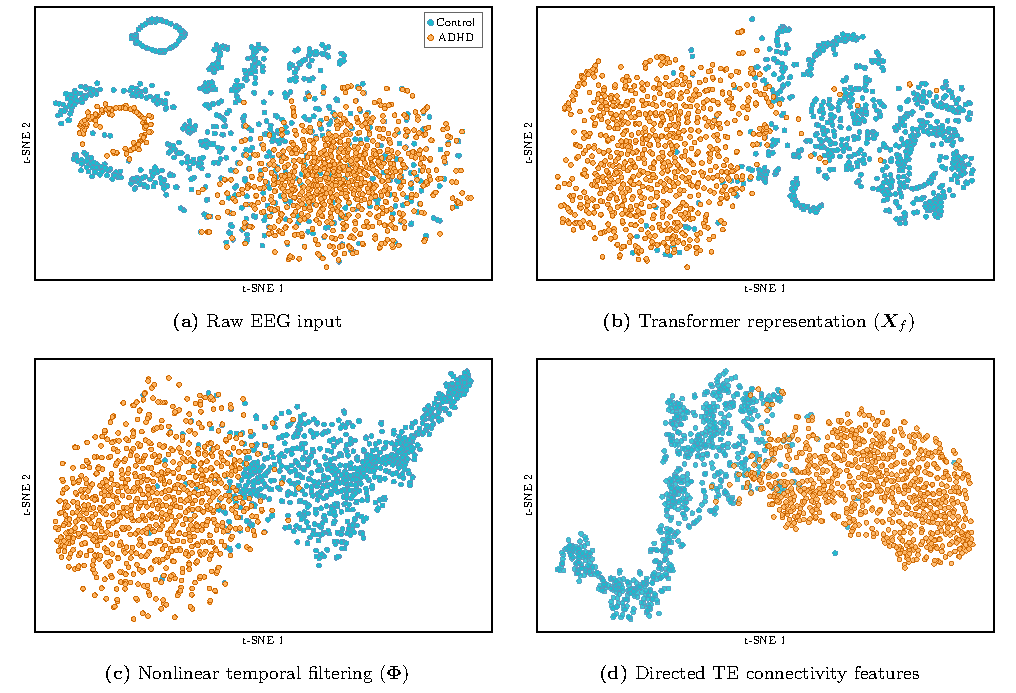
\includegraphics[width=\textwidth]
    {Figures/T-Sne}

    \caption{Evolution of the \gls{eeg} feature space across the main stages of \gls{ctenet}. The t-SNE projections correspond to (a) the raw \gls{eeg} input, (b) Transformer-contextualized channel representations, (c) nonlinear temporal filtering, and (d) directed transfer entropy connectivity features. Blue and orange markers denote Control and \gls{adhd}, respectively.}
    \label{fig:tsne_architecture_stages}
\end{figure}

The quantitative results in Table~\ref{tab:diagnostic_organization} corroborate the progressive organization observed in the t-SNE projections. The raw \gls{eeg} space showed weak diagnostic structure, with participant centroids from the same class being nearly as distant as those from different classes. Transformer contextualization improved this organization primarily at the participant level, despite the remaining overlap among individual windows. Nonlinear temporal filtering further enhanced both window- and centroid-level organization.

The Transfer Entropy representation achieved the most favorable result for all three metrics. Although some \gls{adhd}--control overlap remained, the simultaneous increase in both silhouette coefficients and reduction in the centroid-distance ratio indicate a more coherent diagnostic organization. Differences among stages were significant for all metrics (Friedman tests, $p\leq 3\times10^{-6}$), and the comparisons between the raw \gls{eeg} and Transfer Entropy spaces remained significant after Holm correction ($p_{\mathrm{Holm}}=0.0117$). Therefore, the qualitative t-SNE pattern is supported by quantitative evidence computed in the
standardized PCA space and does not depend exclusively on the two-dimensional visualization. These findings also indicate that the subsequent reduction in within-subject dispersion was not achieved at the expense of \gls{adhd}--control organization.

\begin{table}[htbp]
\centering
\caption{Diagnostic organization across the representation stages of \gls{ctenet}. Values correspond to averages across the ten training repetitions after averaging the five test folds within each repetition.}
\label{tab:diagnostic_organization}

\begin{threeparttable}
\small
\renewcommand{\arraystretch}{1.20}
\setlength{\tabcolsep}{5pt}

\begin{tabular*}{\textwidth}{@{\extracolsep{\fill}}l
    S[table-format=1.4]S[table-format=1.4]S[table-format=1.4]@{}}
\toprule

\textbf{Representation}
& \multicolumn{2}{c}{\textbf{Class silhouette} $\uparrow$}
& {\textbf{Same/different}} \\

\cmidrule(lr){2-3}

\textbf{stage}
& {\textbf{Window level}}
& {\textbf{Centroid level}}
& {\textbf{class ratio}\,$\downarrow$} \\

\midrule

Raw \gls{eeg}                  & 0.0558 & 0.0210 & 0.9887 \\
Transformer ($X_f$)      & 0.0712 & 0.2640 & 0.7056 \\
Temporal filter ($\Phi$) & 0.1326 & 0.3316 & 0.6326 \\
Transfer Entropy         & \bfseries 0.2148 & \bfseries 0.3557 & \bfseries 0.6031 \\

\bottomrule
\end{tabular*}

\begin{tablenotes}[flushleft]
\footnotesize
\item \textit{Note:} Arrows indicate the direction of more favorable
diagnostic organization: higher silhouette coefficients ($\uparrow$) and lower
same-to-different class centroid-distance ratios ($\downarrow$). All
quantities were computed in the standardized PCA space described in
Section~\ref{subsec:representation_analysis}. Bold values indicate the most
favorable value for each measure, obtained in every case at the directed
Transfer Entropy stage.
\end{tablenotes}
\end{threeparttable}
\end{table}
%----------------------------------------------------------
\subsubsection{Reduction of Within-Subject Variability across \gls{ctenet} Representations}


Figure~\ref{fig:within_subject_dispersion} shows the evolution of normalized within-subject dispersion across the four representation stages. The raw \gls{eeg} representation exhibited substantial between-participant heterogeneity, including several subjects with markedly elevated dispersion. Transformer contextualization produced a narrower distribution across participants, but did not reduce the median dispersion relative to raw \gls{eeg}. In contrast, nonlinear temporal filtering initiated a reduction, which became most pronounced after the directed Transfer Entropy transformation.

\begin{figure}[htbp]
    \centering
    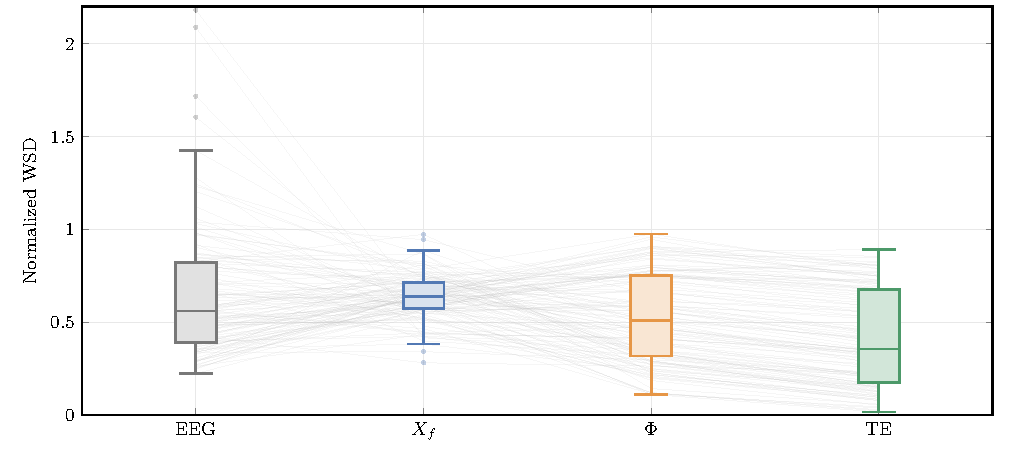
\includegraphics[width=\textwidth]{Figures/Dispersion.pdf}
    \caption{Within-subject dispersion across the four representation stages of \gls{ctenet}. Boxplots summarize the normalized subject-level
    dispersion after averaging across ten random seeds, while the faint trajectories connect the four representations of each participant.
    Lower values indicate a more compact organization of \gls{eeg} windows within the same participant. The directed Transfer Entropy
    representation exhibited the lowest overall within-subject dispersion.}
    \label{fig:within_subject_dispersion}
\end{figure}
% %----------------------------------------------------------

The Transfer Entropy representation exhibited the lowest median and mean within-subject dispersion among all stages. Relative to raw \gls{eeg}, the median reduction was 38.35\%, with lower dispersion observed in 76 of the 120 participants. This reduction was statistically supported by the Holm-corrected Wilcoxon comparison ($p_{\mathrm{Holm}}=1.09\times10^{-4}$), while the overall differences among representation stages were significant according to the Friedman test ($\chi^2(3)=69.11$, $p=6.62\times10^{-15}$). Although individual trajectories were heterogeneous and the reduction was not observed for every participant, the overall pattern indicates that directed-connectivity estimation produces a more compact organization of windows belonging to the same child.

{A reduction in within-subject dispersion would not be meaningful if it resulted from a general collapse of the representation space. Two complementary findings argue against a simple global collapse. First, the dispersion measure is normalized by the mean pairwise distance across the complete test set within each representation; therefore, a uniform contraction would reduce both the within-subject and reference distances proportionally and would not, by itself, explain the observed change. Second, the Transfer Entropy stage simultaneously exhibited the most favorable diagnostic organization, including the highest window- and centroid-level silhouette coefficients and the lowest same-class to different-class centroid-distance ratio (Table~\ref{tab:diagnostic_organization}). The cosine-distance analysis without PCA separately confirmed that the reduction in within-subject dispersion was not an artifact of the PCA basis or Euclidean geometry. Together, these findings argue against a simple global feature collapse, although they do not exclude every possible form of representation degeneration.}

\subsubsection{Robustness to the comparison space}

To determine whether the observed reduction in within-subject dispersion depended on the dimensionality or geometry selected for the analysis, the representations were evaluated using PCA projections with 15, 30, and 60 components, as well as pairwise cosine distances computed directly from the standardized features without PCA. As shown in Fig.~\ref{fig:robustness_representation_space}, the intermediate Transformer representation exhibited a moderate increase in dispersion under the PCA-based configurations, whereas the nonlinear temporal filtering stage produced a consistent reduction relative to the raw \gls{eeg} representation. Most importantly, the Transfer Entropy representation yielded the largest reduction under all evaluated comparison spaces, with median changes of approximately 37--45\%. The similar results obtained with 15, 30, and 60 principal components indicate that the effect is not determined by the specific PCA dimensionality selected for the main analysis.

% %----------------------------------------------------------
\begin{figure}[htbp]
    \centering
    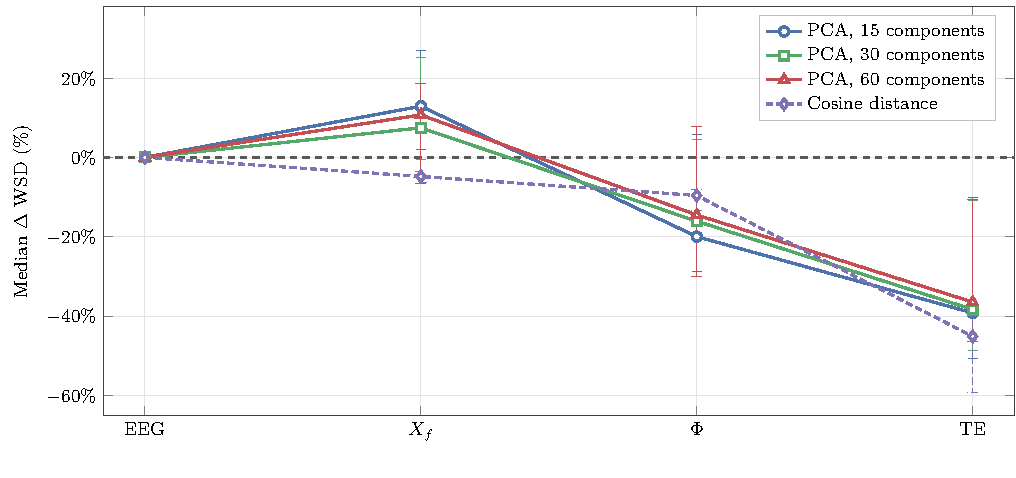
\includegraphics[width=\textwidth]{Figures/Robustness.pdf}
    \caption{Robustness of within-subject dispersion reduction across alternative comparison spaces. The median percentage change in normalized within-subject dispersion is shown relative to the raw \gls{eeg} representation for PCA projections with 15, 30, and 60 components, and for pairwise cosine distances computed without PCA. Negative values indicate a reduction in within-subject dispersion, while the vertical bars represent 95\% bootstrap confidence intervals.}
    \label{fig:robustness_representation_space}
\end{figure}
% %----------------------------------------------------------
The preservation of the effect when using cosine distances without PCA further indicates that the reduction is not an artifact introduced by the linear projection or by the Euclidean centroid-based geometry. Although the magnitude of the reduction varied across comparison spaces, its direction remained consistent at the Transfer Entropy stage. This result supports the interpretation that the directed-connectivity transformation produces a more compact organization of the windows belonging to the same participant. Therefore, the main finding of reduced within-subject dispersion is robust to alternative dimensionality-reduction settings and distance definitions, complementing the subject-level Friedman and Wilcoxon analyses reported previously.

\subsubsection{Stability of Directed Transfer Entropy Representations}

{Across the out-of-fold test representations, the off-diagonal Transfer Entropy coefficients ranged from $-0.0801$ to $0.5156$. Negative estimates accounted for $10.06\%$ of the coefficients, and no non-finite values were observed. The negative values were retained rather than clipped because non-negativity is not explicitly imposed by the finite-sample matrix-based estimator and should not be interpreted as negative information transfer.}

{Across the 120 participants, the mean Spearman correlation between each window-level Transfer Entropy vector and the mean of the participant's remaining windows was 0.743 (95\% CI: 0.733--0.753). The mean Jaccard similarity for the strongest 10\% of directed connections was 0.492 (95\% CI: 0.474--0.509). These results indicate that the global ranking of directed connections remained comparatively stable across windows, whereas the exact composition of the strongest connections showed greater variability.}

\subsubsection{Subject-level analysis of directed connectivity patterns}

To qualitatively illustrate subject-level connectivity patterns associated with correct and incorrect model decisions, four participants were selected from the held-out test partition using their participant-level classification probabilities. These probabilities were obtained by averaging the predicted \gls{adhd} probabilities across all windows of each participant. The correctly classified Control and \gls{adhd} cases corresponded to the lowest and highest mean \gls{adhd} probabilities within their respective classes, whereas the misclassified Control and \gls{adhd} cases corresponded to the opposite extremes. The connectivity maps themselves were not used in the selection procedure. For each selected participant, the displayed Transfer Entropy matrix was obtained by averaging the connectivity matrices across all available \gls{eeg} windows.
% %----------------------------------------------------------------------------------
\begin{figure}[H]
    \centering

    \begin{minipage}[c]{0.44\textwidth}
        \centering
        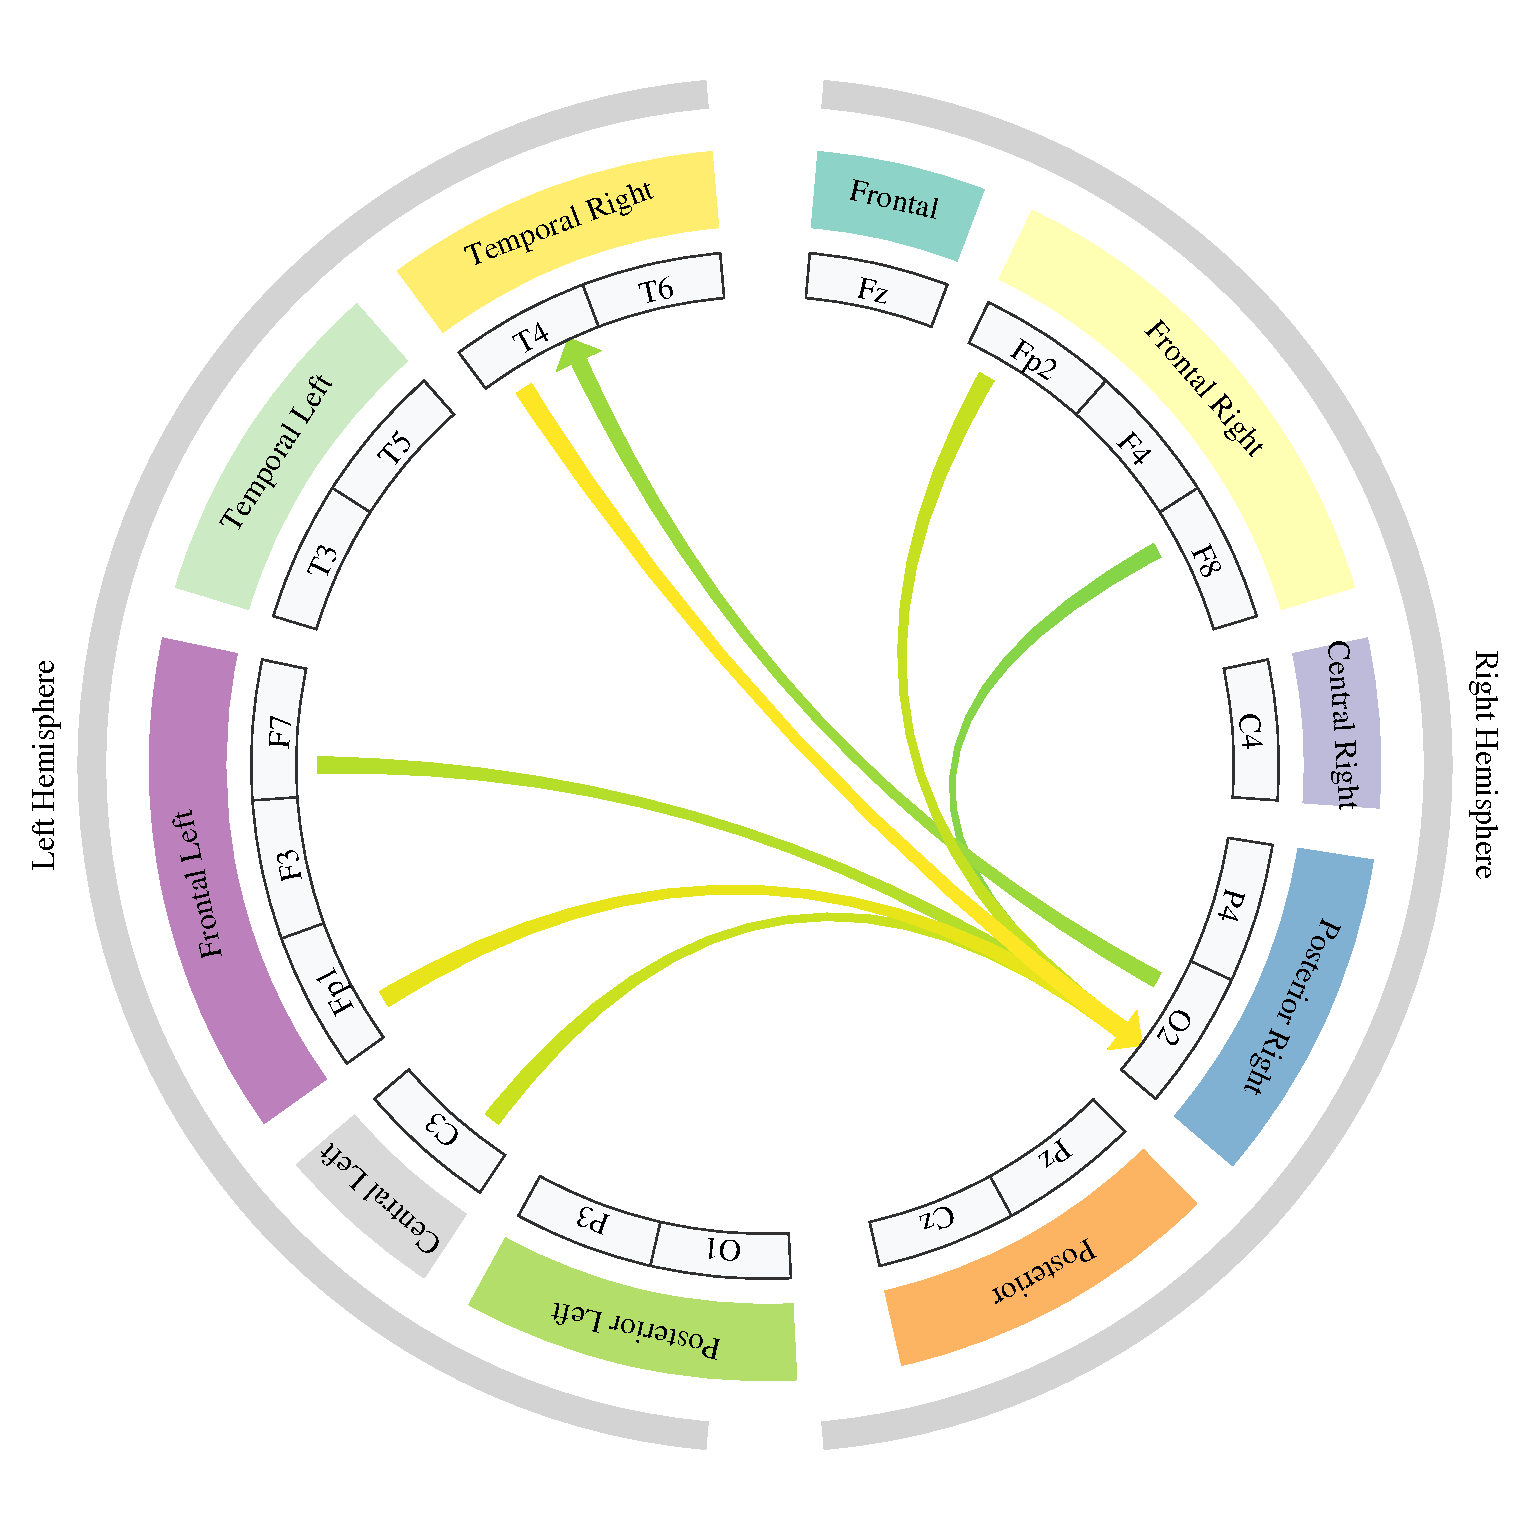
\includegraphics[
            width=\linewidth
        ]{Figures/best_control_v306_normalized.pdf}

        \vspace{1mm}

        {\small
        (a) Correctly classified Control (\texttt{Sv306}).}
    \end{minipage}
    \hfill
    \begin{minipage}[c]{0.44\textwidth}
        \centering
        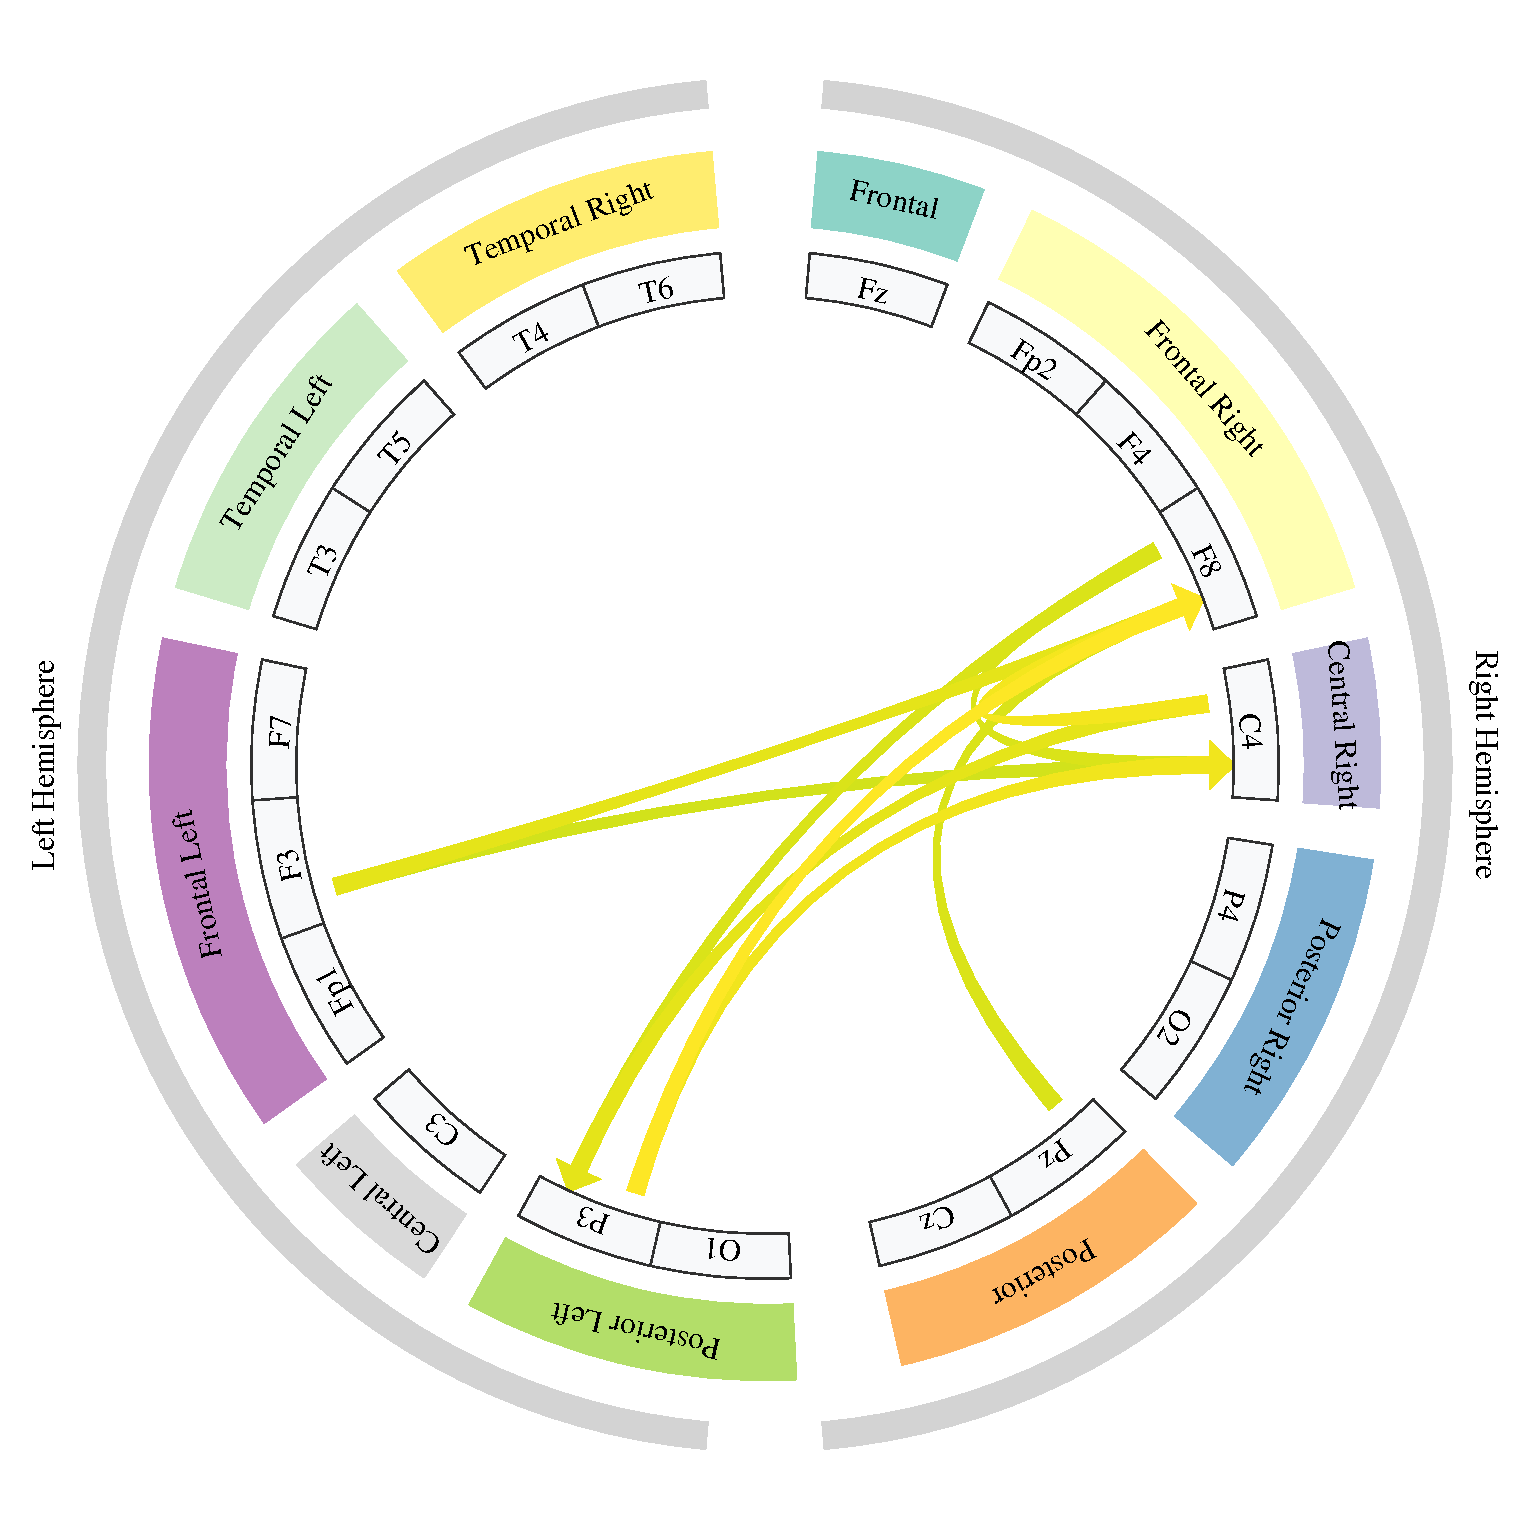
\includegraphics[
            width=\linewidth
        ]{Figures/best_tdah_v284_normalized.pdf}

        \vspace{1mm}

        {\small
        (b) Correctly classified \gls{adhd} (\texttt{Sv284}).}
    \end{minipage}
    \hfill
    \begin{minipage}[c]{0.055\textwidth}
        \centering

        \begin{tikzpicture}
            \begin{axis}[
                hide axis,
                scale only axis,
                width=0pt,
                height=6.5cm,
                colormap/viridis,
                point meta min=0,
                point meta max=1,
                colorbar,
                colorbar style={
                    height=5.5cm,
                    width=0.30cm,
                    ytick={0,0.2,0.4,0.6,0.8,1},
                    yticklabels={0.0,0.2,0.4,0.6,0.8,1.0},
                    yticklabel style={
                        font=\scriptsize
                    }
                }
            ]

            \addplot[
                draw=none,
                point meta=explicit
            ]
            coordinates {
                (0,0) [0]
                (1,1) [1]
            };

            \end{axis}
        \end{tikzpicture}
    \end{minipage}

    \caption{
        Directed Transfer Entropy connectivity patterns for
        representative correctly classified subjects.
        Only the top 5\% of the strongest directed connections are shown.
        Arrow direction indicates the estimated direction of information
        transfer, while color represents the normalized TE magnitude
        using a shared range.
    }

    \label{fig:correct_subjects_te}
\end{figure}

% %----------------------------------------------------------------------------------

\begin{figure}[H]
    \centering

    \begin{minipage}[c]{0.445\textwidth}
        \centering
        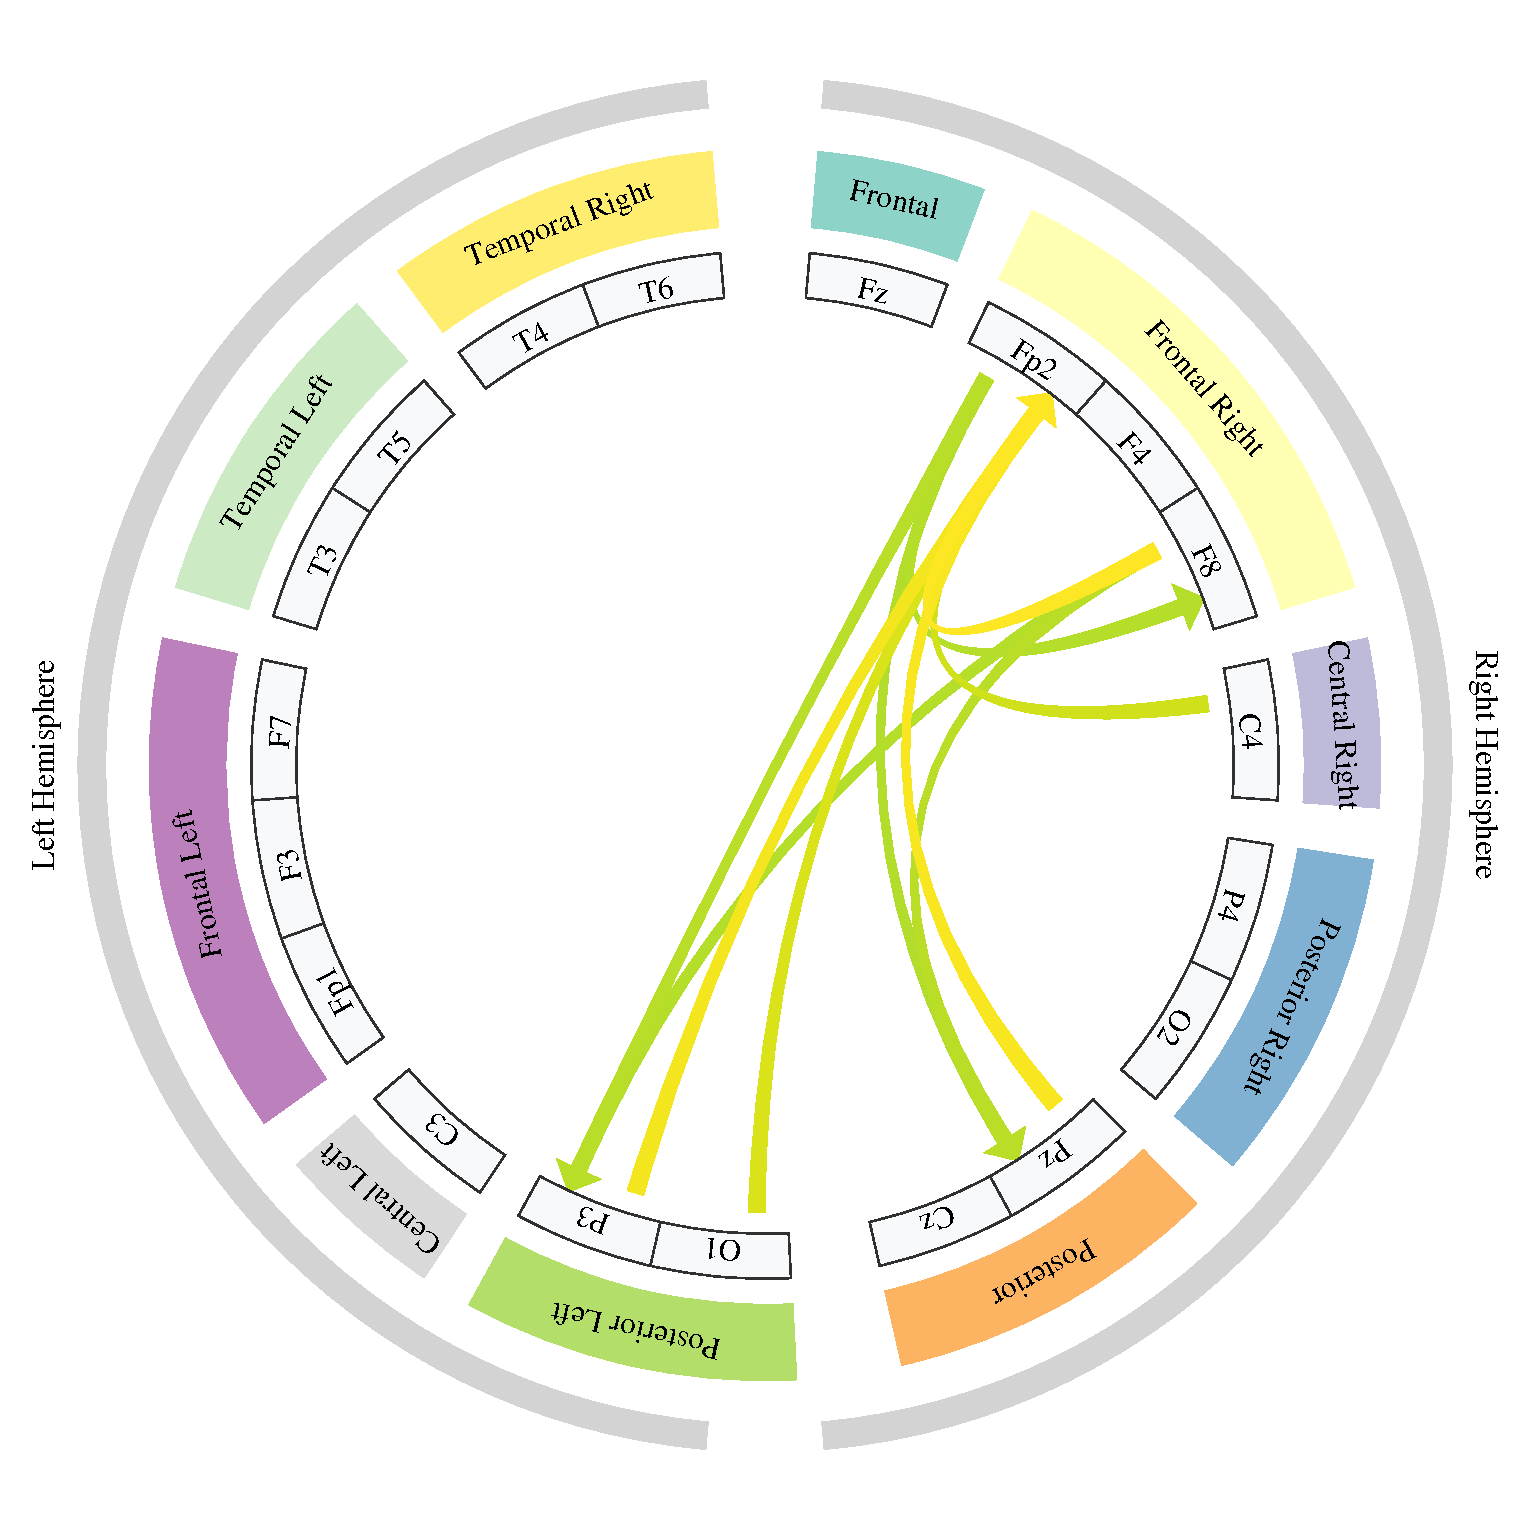
\includegraphics[
            width=\linewidth
        ]{Figures/misclassified_control_v297_normalized.pdf}

        \vspace{1mm}

        {\small
        (a) Misclassified Control (\texttt{Sv297}).}
    \end{minipage}
    \hfill
    \begin{minipage}[c]{0.445\textwidth}
        \centering
        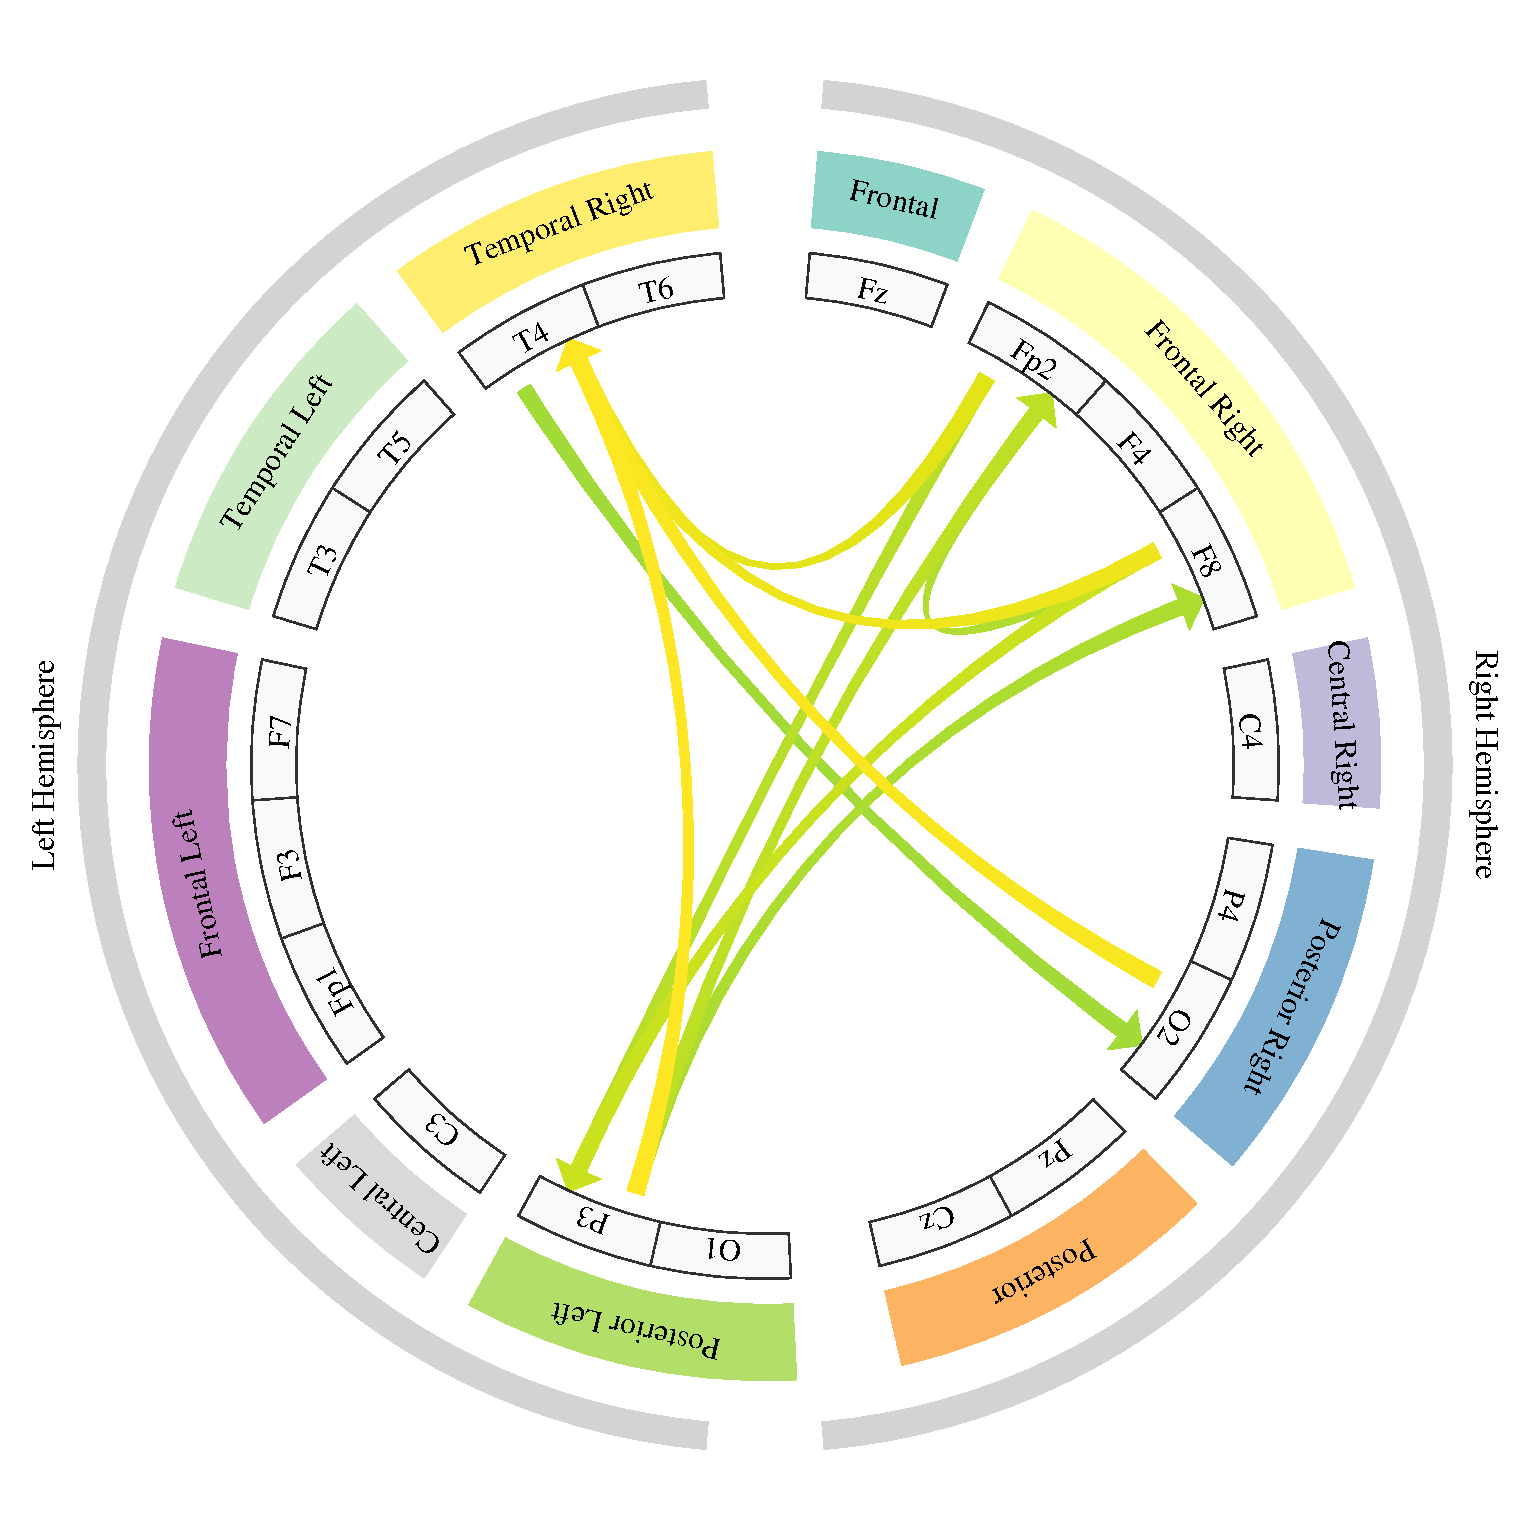
\includegraphics[
            width=\linewidth
        ]{Figures/misclassified_tdah_v27p_normalized.pdf}

        \vspace{1mm}

        {\small
        (b) Misclassified \gls{adhd} (\texttt{Sv27p}).}
    \end{minipage}
    \hfill
    \begin{minipage}[c]{0.045\textwidth}
        \centering

        \begin{tikzpicture}
            \begin{axis}[
                hide axis,
                scale only axis,
                width=0pt,
                height=5.5cm,
                colormap/viridis,
                point meta min=0,
                point meta max=1,
                colorbar,
                colorbar style={
                    height=5.5cm,
                    width=0.22cm,
                    ytick={0,0.2,0.4,0.6,0.8,1},
                    yticklabels={0.0,0.2,0.4,0.6,0.8,1.0},
                    yticklabel style={
                        font=\scriptsize
                    }
                }
            ]

            \addplot[
                draw=none,
                point meta=explicit
            ]
            coordinates {
                (0,0) [0]
                (1,1) [1]
            };

            \end{axis}
        \end{tikzpicture}
    \end{minipage}

    \caption{
        Directed Transfer Entropy connectivity patterns for
        representative misclassified subjects.
        Only the top 5\% of the strongest directed connections are shown.
        Arrow direction indicates the estimated direction of information
        transfer, while color represents the normalized TE magnitude
        using a shared range.
    }

    \label{fig:misclassified_subjects_te}
\end{figure}
%----------------------------------------------------------
\subsection{Summary}
\label{sec:Conclu3}

In this chapter, we proposed \gls{ctenet}, an end-to-end architecture that extends the kernel-based Transfer Entropy (TE) framework through Transformer-based contextualization for pediatric attention-deficit/hyperactivity disorder (\gls{adhd}) classification. Building on the directed-dependency modeling developed with \gls{tektenet}, the proposed architecture integrates global contextualization, channel-wise nonlinear temporal filtering, Takens delay-coordinate reconstruction, and differentiable kernel TE estimation. This combination provides a supervised representation of nonlinear, time-delayed, and directed predictive dependencies while enabling the inspection of how \gls{eeg} Windows are organized within and across participants.

The experimental evaluation involved 120 children, five fixed subject-wise folds, and ten random training repetitions. \gls{ctenet} achieved a window-level accuracy of $80.9 \pm 1.7\%$ and a participant-level accuracy of $83.4\%$ (95\% CI: 78.2--88.2), with a participant-level ROC-AUC of $90.2\%$ (95\% CI: 85.1--94.6). These results support competitive classification performance under an evaluation in which test participants were absent from the corresponding training and validation subsets. Participant-level comparisons did not establish statistically significant differences from \gls{eeg}Net, ShallowConvNet, T-GARNet, or IMC-BGT after Holm correction, whereas the comparison with MultiStream favored \gls{ctenet}. Accordingly, the contribution is supported by the combination of predictive performance and an explicit directed-connectivity representation, without implying universal superiority over the evaluated classifiers.

The ablation analysis clarified the roles of the principal architectural components. Removing the Transformer produced the largest performance reductions, with a significant participant-level difference in favor of the complete model. Replacing the TE module with temporal mean pooling also reduced the point estimates, although the participant-level difference was not statistically significant. These findings support the predictive contribution of global contextualization and more moderate evidence for the incremental predictive benefit of TE. The TE module nevertheless supplies the nonlinear, delayed, and directed representation that enables the subsequent connectivity and feature-space analyses.

The representation analysis showed progressively more favorable class organization across the learned stages. The TE representation achieved the highest window- and centroid-level silhouette coefficients and the lowest normalized within-subject dispersion. Relative to raw \gls{eeg}, the median dispersion reduction was $38.35\%$, with lower dispersion in 76 of the 120 participants. The direction of this result persisted across the evaluated PCA dimensionalities and the cosine-distance analysis without PCA. These controls support consistency across the tested comparison spaces, although they do not establish independence from representation-specific standardization. Thus, the findings indicate that a discriminatively learned directed-connectivity space can reduce window-specific variability while retaining class-related structure.

Complementary connectivity analyses characterized both the interpretability and the stability of this representation. Across participants, the mean window-to-remaining-window Spearman correlation was $0.743$, whereas the mean Jaccard similarity for the strongest $10\%$ of connections was $0.492$. The overall ranking of connections was therefore more consistent across windows than the exact membership of the strongest subset. Selected individual maps illustrated different organizations in correctly and incorrectly classified cases, but did not establish population-level biomarkers. Because the Transformer contextualizes the channel representations before TE estimation, these coefficients describe directed predictive dependencies between learned channel-indexed coordinates, rather than direct interactions between anatomically localized cortical sources.

The sensitivity analyses also delineated the scope of the findings. Frequency filtering combined with quality screening reduced participant-level performance, while common average reference preserved classification performance but substantially changed the learned connections. Predictive robustness and connectivity stability must therefore be assessed separately. Together with the single-cohort design, unavailable participant-linked demographic and medication information, and the need for fully nested model selection, these findings limit clinical and physiological generalization. Overall, this chapter advances the thesis from directed-dependency estimation toward contextualized and inspectable \gls{eeg} representation learning, providing proof-of-concept evidence in a pediatric classification task that complements the preceding motor-imagery studies.
\chapter{Final Remarks}


\section{Conclusions}
This thesis investigated how connectivity-based representations can be integrated with deep learning to support EEG decoding while making the information used by the models more accessible to analysis. The three contributions follow a methodological progression: spatially structured functional-connectivity imaging with EEG-GCIRNet, differentiable nonlinear and directed-dependency estimation with \gls{tektenet}, and contextualized directed-connectivity learning with CTE-Net. Together, they support connectivity as a useful representation for both prediction and model inspection. Their contributions concern learned representations and their empirical behavior; they do not establish that sensor-level connectivity recovers the underlying cortical mechanisms.

The first objective was addressed through EEG-GCIRNet, which combines Gaussian functional-connectivity representations, electrode-topographic imaging, and a variational autoencoder for joint reconstruction and classification. The framework achieved an average accuracy of $81.82\%$ on the binary GigaScience evaluation and $75.20\%$ in the five-class EEGMMIDB scenario. In the reported GigaScience analysis, improvements were particularly marked among participants with lower EEGNet baseline performance, and no evaluated participant remained below the study's $60\%$ accuracy threshold. This supports the usefulness of spatially organized connectivity features and latent regularization for the evaluated motor-imagery tasks. It does not imply a general elimination of poor BCI performance outside these data and protocols. Reconstruction, latent-space, and relevance-map analyses provided complementary descriptions of the learned representations, while the more limited pediatric ADHD results showed that strong subject-specific decoding does not automatically translate into generalization to unseen participants.

The second objective was addressed through \gls{tektenet}, which integrates nonlinear temporal filtering, Takens delay-coordinate reconstruction, and kernel-based TE estimation within a differentiable classification architecture. This contribution makes nonlinear, delayed, and directional predictive relationships available to end-to-end learning. Experiments on semi-synthetic data provided controlled evidence concerning the imposed interaction structures and sensitivity to noise. On the official BCI Competition IV-2a test data, the chapter reported an accuracy of $80.12\%$. Temporal, spectral, and connectivity analyses further characterized the task intervals, learned frequency responses, and subject-specific patterns associated with decoding. These results support the methodological value of integrating state-space reconstruction and information-theoretic estimation. The persistence of low-performing participants and the more limited ADHD results also show that directed-dependency modeling alone does not resolve all sources of EEG variability.

The third objective was addressed through CTE-Net and its representation-level evaluation. The model combines Transformer-based contextualization with differentiable directed-connectivity estimation and was assessed using subject-wise partitions and repeated training. Participant-level accuracy reached $83.4\%$, with a ROC-AUC of $90.2\%$, while the TE stage exhibited a median within-subject dispersion reduction of $38.35\%$ relative to raw EEG in the specified analysis space. The ablation findings supported the contribution of the Transformer and more moderate evidence for an additional predictive benefit from TE. The resulting contribution is therefore twofold: competitive classification of unseen participants within the evaluated cohort, and an inspectable representation through which class organization, within-participant variability, and connection stability can be examined. This pediatric study extends the methodological investigation beyond motor imagery, but does not by itself establish improved online BCI control or subject-independent motor-imagery decoding.

Across the three objectives, the evidence supports complementary roles for connectivity and representation learning. EEG-GCIRNet introduces spatial organization into the decoding pipeline; \gls{tektenet} adds nonlinear temporal and directional structure; and CTE-Net examines the effect of global contextualization on the learned directed representation. These constitute related methodological contributions rather than a controlled ranking of three successive architectures. Their reported accuracies arise from different datasets, tasks, preprocessing choices, model-selection procedures, and evaluation units. Consequently, numerical differences across chapters cannot be attributed exclusively to architectural changes. Establishing such effects requires a common experimental protocol.

The thesis also demonstrates that interpretability must be evaluated separately from predictive performance. Relevance maps, reconstructed topographies, learned filters, and directed-connectivity patterns reveal aspects of model behavior, but anatomical plausibility alone does not rule out artifacts, confounding, or spatial mixing. In CTE-Net, relatively preserved classification under rereferencing coexisted with substantial changes in the estimated connections. Moreover, reducing within-subject dispersion in a transformed feature space is not equivalent to removing physiological nonstationarity from the original EEG. These distinctions define the scope of the evidence and prevent predictive, representational, and physiological conclusions from being treated as interchangeable.

Overall, the thesis contributes a set of connectivity-based deep learning methods and analyses for studying EEG decoding under subject-specific and subject-wise evaluation settings. The findings support the use of structured connectivity representations to combine useful predictive performance with explicit investigation of spatial, temporal, and directional relationships. Generalization across independent cohorts, stability across recording conditions, and prospective utility remain to be established. The resulting foundation supports further development of interpretable EEG decoders for BCI research and related neurodevelopmental classification applications.

\section{Future Work}
The next stage should establish a unified evaluation of EEG-GCIRNet, \gls{tektenet}, CTE-Net, and representative baselines. A shared protocol should specify the same eligible participants, target classes, preprocessing conditions, training budgets, and evaluation units wherever the architectures can be compared. Fully nested cross-validation should isolate hyperparameter optimization within each outer training partition, followed by evaluation on independent cohorts. Subject-specific, cross-session, and subject-independent experiments should be reported separately. Repeated training can quantify optimization variability, while participant-level inference should retain the participant as the independent observational unit. Such a design would clarify which benefits arise from connectivity construction, temporal reconstruction, contextualization, or other experimental choices.

Preprocessing sensitivity should be investigated through controlled experiments that separate the effects of filtering, artifact handling, window exclusion, and reference choice. The combined filtering and quality-screening analysis in CTE-Net cannot identify the individual contribution of each operation. A factorial evaluation, with data-dependent thresholds estimated exclusively from training participants, would help resolve this uncertainty. Connectivity agreement and classification performance should both be reported under each condition. Additional evaluation of surface Laplacian and, where suitable acquisition information is available, source-space representations could examine sensitivity to spatial mixing without assuming that these procedures eliminate all confounding influences.

The directed-connectivity estimator should also be evaluated more extensively under controlled conditions. Simulations with known interaction delays, common drivers, indirect pathways, changing coupling strengths, and nonstationary dynamics would help distinguish sensitivity to predictive dependence from recovery of a specified interaction structure. Multivariate or conditional TE formulations could be investigated to account for observed common influences and indirect pairwise effects. Finite-sample bias, negative estimates, and sensitivity to embedding dimensions and kernel parameters require explicit characterization. Any interpretation in terms of interventional or mechanistic causality would require additional assumptions and experimental evidence beyond the observational sensor-level analyses developed here.

Architectural extensions should test whether explicit temporal position information improves contextualization before directed-dependency estimation. Absolute or relative positional representations can be compared with the present CTE-Net design, in which temporal order is modeled by the subsequent temporal filters and Takens reconstruction. Multiband connectivity modules could assess whether frequency-resolved dependencies offer additional predictive or interpretive value. Sparse connectivity representations and graph-based classifiers are further candidates, provided that their benefits are evaluated through controlled ablations and repeated training. Greater architectural complexity should be justified by measurable gains in generalization, stability, or interpretability.

Further work should characterize the reproducibility of the learned representations across windows, training seeds, recording sessions, and cohorts. Group-level connection analyses should use independent participants and appropriate multiple-comparison control. Representation comparisons should include sensitivity to normalization and projection, alongside perturbation-based tests that assess whether the highlighted features affect predictions. Subject-balanced sampling or weighting should be evaluated to reduce the unequal influence of recording duration during training. Transfer learning and domain adaptation could then be studied under clearly specified access to target-domain data, with target labels reserved from model selection when evaluating generalization to unseen domains.

For pediatric applications, independent datasets should include participant-linked age, sex, medication status, comorbidities, and behavioral measurements. This would enable subgroup evaluation and examination of potential confounding factors that could not be assessed in the present cohort. Larger multi-site studies should evaluate calibration, uncertainty, and sensitivity to acquisition protocols in addition to discrimination. Prospective assessment would be required to determine whether EEG-based outputs provide useful information alongside clinical assessment. The present classification experiments should serve as methodological groundwork for that evaluation.

Finally, practical BCI deployment requires validation beyond offline accuracy. Channel selection, low-rank kernel approximations, and sparse pairwise estimation could reduce the computational burden of directed-connectivity modules. These changes should be assessed for their effects on both predictions and learned connections. Streaming experiments should explicitly restrict inputs to samples available at the decision time and measure end-to-end latency, calibration requirements, and performance across sessions. Closed-loop studies could subsequently evaluate online control, user adaptation, and the behavior of participants who remain difficult to decode in offline analyses.


\section{Academic Products}

The academic products derived from this doctoral research include peer-reviewed journal publications and open-source software implementations that support the reproducibility and extension of the proposed methodologies.

\begin{itemize}
    \item \textbf{Journal Paper:} Gomez-Rivera, A. and Cardona-Álvarez, Y. and Gomez-Morales, O. W. and Alvarez-Meza, A. M. and Castellanos-Domínguez, G. BCI-based real-time processing for implementing deep learning frameworks using \gls{mi} paradigms. Journal of Applied Research and Technology, Oct 30, 2024. \url{https://doi.org/10.22201/icat.24486736e.2024.22.5.2392}
    
    \item \textbf{Journal Paper (Q1):} Gomez-Rivera, A.; Collazos-Huertas, D.F.; Cárdenas-Peña, D.; Álvarez-Meza, A.M.; Castellanos-Dominguez, G. A Gaussian Connectivity-Driven \gls{eeg} Imaging for Deep Learning-Based Motor Imagery Classification. Sensors 2026, 26, 227. \url{https://doi.org/10.3390/s26010227}.
    
    \item \textbf{Journal Paper (Q1):} Gomez-Rivera, A.; Álvarez-Meza, A.M.; Cárdenas-Peña, D.; Orozco-Gutierrez, A. Takens-Based Kernel \gls{te} Connectivity Network for Motor Imagery Classification. Sensors 2025, 25, 7067.  \url{https://doi.org/10.3390/s25227067}

    \item \textbf{Journal Paper (Q1):} Pastrana-Cortés, J. D.; Gomez-Rivera, A.; Álvarez-Meza, A. M.; Gil-Gonzalez, J.; Cárdenas-Peña, D.
    \emph{Temporal Attention and Convolutional Tokenization for Interpretable \gls{eeg}-Based \gls{adhd} Identification in Children.}
    Technologies, 2026, 14(7), Article 392.
    \href{https://doi.org/10.3390/technologies14070392}{https://doi.org/10.3390/technologies14070392}

    \item \textbf{Journal Paper (Q1):} Gomez-Rivera, A.; Pastrana-Cortés, J. D.; Álvarez-Meza, A. M.; Gil-Gonzalez, J.; Cárdenas-Peña, D.
    \emph{Transformer-Based Modeling of Directed Transfer Entropy Connectivity for \gls{eeg}-Based \gls{adhd} Classification in Children.}
    Sensors, 2026, 26, 5786.
    \href{https://doi.org/10.3390/s26185786}{https://doi.org/10.3390/s26185786}
       
\end{itemize}

\subsection{Open-Source Software and Code Repositories}

\begin{itemize}
    \item \textbf{EEG-GCIRNet}: Open-source implementation of the Gaussian connectivity-driven EEG imaging framework proposed in this thesis.  
    \url{https://github.com/alegomezri/EEG-GCIRNet}
    
    \item \textbf{\gls{tektenet}}: Open-source implementation of the Takens-based kernel transfer entropy connectivity network for effective connectivity modeling.  
    \url{https://github.com/alegomezri/TEKTE-Net}
    
    \item \textbf{EEG-TACT}: Open-source implementation of the temporal attention and convolutional tokenization framework for interpretable EEG-based ADHD classification.
    \url{https://github.com/alegomezri/EEG-TACT}

    \item \textbf{CTE-Net}: Open-source implementation of the contextualized Transfer Entropy network for learning nonlinear and directed EEG connectivity representations.
    \url{https://github.com/alegomezri/CTE-Net}

\end{itemize}

\Needspace{7\baselineskip}
\subsection{Patents and Technology Transfer}

\begin{itemize}
    \item \textbf{Granted Patent:} NC2022/0007405.
    \emph{Método y sistema para la sincronización de marcadores asociados a sistemas de interfaz cerebro--computador.}
    Granted by the Superintendence of Industry and Commerce (SIC), Colombia,
    through Resolution No.~48299 of June 25, 2026. Patent term: 2022--2042.
\end{itemize}


%Inicio del apéndice o anexos
% \begin{appendix}
% \include{Appendices/Appendix}%
% \end{appendix}

%Permite visualizar la bibliografía en la tabla de contenido
\addcontentsline{toc}{chapter}{References} %Literatura Citada

\let\OLDthebibliography=\thebibliography
\def\thebibliography#1{\OLDthebibliography{#1}}
{\scriptsize
%\pagestyle{plain}
\bibliographystyle{dtvstyle}
% Nombre del documento donde se almacenan las referencias
\bibliography{References}
\nocite{*}
\cleardoublepage
}

\end{document}
